\documentclass[a4paper]{book}
\usepackage{a4wide}
\usepackage{makeidx}
\usepackage{fancyhdr}
\usepackage{graphicx}
\usepackage{float}
\usepackage{alltt}
\usepackage{doxygen}
\makeindex
\setcounter{tocdepth}{1}
\setlength{\footrulewidth}{0.4pt}
\begin{document}
\begin{titlepage}
\vspace*{7cm}
\begin{center}
{\Large Covered Reference Manual\\[1ex]\large 0.1.1}\\
\vspace*{1cm}
{\large Generated by Doxygen 1.2.16}\\
\vspace*{0.5cm}
{\small Tue Jul 2 17:36:55 2002}\\
\end{center}
\end{titlepage}
\clearemptydoublepage
\pagenumbering{roman}
\tableofcontents
\clearemptydoublepage
\pagenumbering{arabic}
\chapter{Covered: Verilog Code-Coverage Analyzer}
\label{index}\begin{CompactItemize}
\item 
{\bf Introduction} {\rm (p.\,\pageref{page_intro})}\item 
{\bf How does Covered work?} {\rm (p.\,\pageref{page_howitworks})}\item 
{\bf Look here for the latest Covered news!} {\rm (p.\,\pageref{page_news})}\item 
{\bf What is on the Covered todo list} {\rm (p.\,\pageref{page_todo})}\item 
{\bf Downloading and Installing Covered} {\rm (p.\,\pageref{page_download})}\item 
{\bf Reporting Covered Bugs} {\rm (p.\,\pageref{page_bugs})}\end{CompactItemize}

\chapter{Covered Module Index}
\section{Covered Modules}
Here is a list of all modules:\begin{CompactList}
\item \contentsline{section}{Output type}{\pageref{group__output__type}}{}
\item \contentsline{section}{Database line types}{\pageref{group__db__types}}{}
\item \contentsline{section}{Compare types for tree matches.}{\pageref{group__tree__fname__comps}}{}
\item \contentsline{section}{Detailedness of reports.}{\pageref{group__report__detail}}{}
\item \contentsline{section}{Vector-specific defines.}{\pageref{group__vector__defs}}{}
\item \contentsline{section}{Expression supplemental field defines and macros.}{\pageref{group__expr__suppl}}{}
\item \contentsline{section}{Modes for reading database file}{\pageref{group__read__modes}}{}
\item \contentsline{section}{Instance/module parameter supplemental field definitions.}{\pageref{group__param__suppl}}{}
\item \contentsline{section}{Expression operations}{\pageref{group__expr__ops}}{}
\item \contentsline{section}{Op\_\-tables}{\pageref{group__op__tables}}{}
\item \contentsline{section}{Comparison\_\-types}{\pageref{group__comparison__types}}{}
\item \contentsline{section}{Lexer\_\-val\_\-types}{\pageref{group__lexer__val__types}}{}
\end{CompactList}

\chapter{Covered Compound Index}
\section{Covered Compound List}
Here are the classes, structs, unions and interfaces with brief descriptions:\begin{CompactList}
\item\contentsline{section}{{\bf case\_\-stmt\_\-s} }{\pageref{structcase__stmt__s}}{}
\item\contentsline{section}{{\bf exp\_\-link\_\-s} }{\pageref{structexp__link__s}}{}
\item\contentsline{section}{{\bf expr\_\-stmt\_\-u} }{\pageref{unionexpr__stmt__u}}{}
\item\contentsline{section}{{\bf expression\_\-s} }{\pageref{structexpression__s}}{}
\item\contentsline{section}{{\bf include\_\-stack\_\-t} }{\pageref{structinclude__stack__t}}{}
\item\contentsline{section}{{\bf inst\_\-parm\_\-s} }{\pageref{structinst__parm__s}}{}
\item\contentsline{section}{{\bf keyword} }{\pageref{structkeyword}}{}
\item\contentsline{section}{{\bf mod\_\-inst\_\-s} }{\pageref{structmod__inst__s}}{}
\item\contentsline{section}{{\bf mod\_\-link\_\-s} }{\pageref{structmod__link__s}}{}
\item\contentsline{section}{{\bf mod\_\-parm\_\-s} }{\pageref{structmod__parm__s}}{}
\item\contentsline{section}{{\bf module\_\-s} }{\pageref{structmodule__s}}{}
\item\contentsline{section}{{\bf sig\_\-exp\_\-bind\_\-s} }{\pageref{structsig__exp__bind__s}}{}
\item\contentsline{section}{{\bf sig\_\-link\_\-s} }{\pageref{structsig__link__s}}{}
\item\contentsline{section}{{\bf signal\_\-s} }{\pageref{structsignal__s}}{}
\item\contentsline{section}{{\bf statement\_\-s} }{\pageref{structstatement__s}}{}
\item\contentsline{section}{{\bf static\_\-expr\_\-s} }{\pageref{structstatic__expr__s}}{}
\item\contentsline{section}{{\bf statistic\_\-s} }{\pageref{structstatistic__s}}{}
\item\contentsline{section}{{\bf stmt\_\-iter\_\-s} }{\pageref{structstmt__iter__s}}{}
\item\contentsline{section}{{\bf stmt\_\-link\_\-s} }{\pageref{structstmt__link__s}}{}
\item\contentsline{section}{{\bf stmt\_\-loop\_\-link\_\-s} }{\pageref{structstmt__loop__link__s}}{}
\item\contentsline{section}{{\bf str\_\-link\_\-s} }{\pageref{structstr__link__s}}{}
\item\contentsline{section}{{\bf symtable\_\-s} }{\pageref{structsymtable__s}}{}
\item\contentsline{section}{{\bf timer\_\-s} }{\pageref{structtimer__s}}{}
\item\contentsline{section}{{\bf tnode\_\-s} }{\pageref{structtnode__s}}{}
\item\contentsline{section}{{\bf vector\_\-s} }{\pageref{structvector__s}}{}
\item\contentsline{section}{{\bf vector\_\-width\_\-s} }{\pageref{structvector__width__s}}{}
\item\contentsline{section}{{\bf vlltype} }{\pageref{structvlltype}}{}
\item\contentsline{section}{{\bf yy\_\-buffer\_\-state} }{\pageref{structyy__buffer__state}}{}
\item\contentsline{section}{{\bf yyltype} }{\pageref{structyyltype}}{}
\item\contentsline{section}{{\bf YYSTYPE} }{\pageref{unionYYSTYPE}}{}
\end{CompactList}

\chapter{Covered File Index}
\section{Covered File List}
Here is a list of all files with brief descriptions:\begin{CompactList}
\item\contentsline{section}{{\bf binding.c} }{\pageref{binding_8c}}{}
\item\contentsline{section}{{\bf binding.h} (Contains all functions for signal/expression binding)}{\pageref{binding_8h}}{}
\item\contentsline{section}{{\bf codegen.c} }{\pageref{codegen_8c}}{}
\item\contentsline{section}{{\bf codegen.h} (Contains functions for generating Verilog code from expression trees)}{\pageref{codegen_8h}}{}
\item\contentsline{section}{{\bf comb.c} }{\pageref{comb_8c}}{}
\item\contentsline{section}{{\bf comb.h} (Contains functions for determining/reporting combinational logic coverage)}{\pageref{comb_8h}}{}
\item\contentsline{section}{{\bf db.c} }{\pageref{db_8c}}{}
\item\contentsline{section}{{\bf db.h} (Contains functions for writing and reading contents of covered database file)}{\pageref{db_8h}}{}
\item\contentsline{section}{{\bf defines.h} (Contains definitions/structures used in the Covered utility)}{\pageref{defines_8h}}{}
\item\contentsline{section}{{\bf expr.c} }{\pageref{expr_8c}}{}
\item\contentsline{section}{{\bf expr.h} (Contains functions for handling expressions)}{\pageref{expr_8h}}{}
\item\contentsline{section}{{\bf fsm.c} }{\pageref{fsm_8c}}{}
\item\contentsline{section}{{\bf fsm.h} (Contains functions for determining/reporting FSM coverage)}{\pageref{fsm_8h}}{}
\item\contentsline{section}{{\bf instance.c} }{\pageref{instance_8c}}{}
\item\contentsline{section}{{\bf instance.h} (Contains functions for handling module instances)}{\pageref{instance_8h}}{}
\item\contentsline{section}{{\bf keywords.c} }{\pageref{keywords_8c}}{}
\item\contentsline{section}{{\bf keywords.h} (Contains functions for checking Verilog keywords)}{\pageref{keywords_8h}}{}
\item\contentsline{section}{{\bf lexer.c} }{\pageref{lexer_8c}}{}
\item\contentsline{section}{{\bf line.c} }{\pageref{line_8c}}{}
\item\contentsline{section}{{\bf line.h} (Contains functions for determining/reporting line coverage)}{\pageref{line_8h}}{}
\item\contentsline{section}{{\bf link.c} }{\pageref{link_8c}}{}
\item\contentsline{section}{{\bf link.h} (Contains functions to manipulate a linked lists)}{\pageref{link_8h}}{}
\item\contentsline{section}{{\bf main.c} }{\pageref{main_8c}}{}
\item\contentsline{section}{{\bf merge.c} }{\pageref{merge_8c}}{}
\item\contentsline{section}{{\bf merge.h} (Contains functions for merge command)}{\pageref{merge_8h}}{}
\item\contentsline{section}{{\bf module.c} }{\pageref{module_8c}}{}
\item\contentsline{section}{{\bf module.h} (Contains functions for handling modules)}{\pageref{module_8h}}{}
\item\contentsline{section}{{\bf parse.c} }{\pageref{parse_8c}}{}
\item\contentsline{section}{{\bf parse.h} (Contains functions for parsing Verilog modules)}{\pageref{parse_8h}}{}
\item\contentsline{section}{{\bf parser.c} }{\pageref{parser_8c}}{}
\item\contentsline{section}{{\bf parser.h} }{\pageref{parser_8h}}{}
\item\contentsline{section}{{\bf parser\_\-misc.c} }{\pageref{parser__misc_8c}}{}
\item\contentsline{section}{{\bf parser\_\-misc.h} (Contains miscellaneous functions declarations and defines used by parser)}{\pageref{parser__misc_8h}}{}
\item\contentsline{section}{{\bf report.c} }{\pageref{report_8c}}{}
\item\contentsline{section}{{\bf report.h} (Contains functions for report command)}{\pageref{report_8h}}{}
\item\contentsline{section}{{\bf score.c} }{\pageref{score_8c}}{}
\item\contentsline{section}{{\bf score.h} (Contains functions for score command)}{\pageref{score_8h}}{}
\item\contentsline{section}{{\bf search.c} }{\pageref{search_8c}}{}
\item\contentsline{section}{{\bf search.h} (Contains functions used for finding Verilog files in the search information provided on the command line)}{\pageref{search_8h}}{}
\item\contentsline{section}{{\bf signal.c} }{\pageref{signal_8c}}{}
\item\contentsline{section}{{\bf signal.h} (Contains functions for handling signals)}{\pageref{signal_8h}}{}
\item\contentsline{section}{{\bf stat.c} }{\pageref{stat_8c}}{}
\item\contentsline{section}{{\bf stat.h} (Contains functions for handling coverage statistics)}{\pageref{stat_8h}}{}
\item\contentsline{section}{{\bf symtable.c} }{\pageref{symtable_8c}}{}
\item\contentsline{section}{{\bf symtable.h} (Contains functions for manipulating a symtable structure)}{\pageref{symtable_8h}}{}
\item\contentsline{section}{{\bf toggle.c} }{\pageref{toggle_8c}}{}
\item\contentsline{section}{{\bf toggle.h} (Contains functions for determining/reporting toggle coverage)}{\pageref{toggle_8h}}{}
\item\contentsline{section}{{\bf util.c} }{\pageref{util_8c}}{}
\item\contentsline{section}{{\bf util.h} (Contains miscellaneous global functions used by many functions)}{\pageref{util_8h}}{}
\item\contentsline{section}{{\bf vcd\_\-lexer.c} }{\pageref{vcd__lexer_8c}}{}
\item\contentsline{section}{{\bf vcd\_\-parser.c} }{\pageref{vcd__parser_8c}}{}
\item\contentsline{section}{{\bf vcd\_\-parser.h} }{\pageref{vcd__parser_8h}}{}
\item\contentsline{section}{{\bf vcd\_\-parser\_\-misc.c} }{\pageref{vcd__parser__misc_8c}}{}
\item\contentsline{section}{{\bf vcd\_\-parser\_\-misc.h} (Contains definitions and other header information for VCD parser and lexer)}{\pageref{vcd__parser__misc_8h}}{}
\item\contentsline{section}{{\bf vector.c} }{\pageref{vector_8c}}{}
\item\contentsline{section}{{\bf vector.h} (Contains vector-related functions for signal vectors)}{\pageref{vector_8h}}{}
\end{CompactList}

\chapter{Covered Page Index}
\section{Covered Related Pages}
Here is a list of all related documentation pages:\begin{CompactList}
\item \contentsline{section}{Section 1.  Introduction}{\pageref{page_intro}}{}

\item \contentsline{section}{Section 2.  Project Plan}{\pageref{page_project_plan}}{}

\item \contentsline{section}{Section 3.  Coding Style Guidelines}{\pageref{page_code_style}}{}

\item \contentsline{section}{Section 4.  Development Tools}{\pageref{page_tools}}{}

\item \contentsline{section}{Section 5.  Project \char`\"{}Big Picture\char`\"{}}{\pageref{page_big_picture}}{}

\item \contentsline{section}{Section 6.  Coverage Development Reference}{\pageref{page_code_details}}{}

\item \contentsline{section}{Section 7.  Test and Checkout Procedure}{\pageref{page_testing}}{}

\item \contentsline{section}{Section 8.  Odds and Ends Information}{\pageref{page_misc}}{}

\item \contentsline{section}{Bug List}{\pageref{bug}}{}

\end{CompactList}

\chapter{Covered Module Documentation}
\section{Output type}
\label{group__output__type}\index{Output type@{Output type}}
\subsection*{Defines}
\begin{CompactItemize}
\item 
\#define {\bf FATAL}\ 1
\item 
\#define {\bf WARNING}\ 2
\item 
\#define {\bf NORMAL}\ 3
\end{CompactItemize}


\subsection{Detailed Description}
The following defines are used by the print\_\-output function to determine what type of output to generate and whether the output should or should not be suppressed. 

\subsection{Define Documentation}
\index{output_type@{output\_\-type}!FATAL@{FATAL}}
\index{FATAL@{FATAL}!output_type@{output\_\-type}}
\subsubsection{\setlength{\rightskip}{0pt plus 5cm}\#define FATAL\ 1}\label{group__output__type_a0}


Indicates that the specified error is fatal and will cause the program to immediately stop. Cannot be suppressed. \index{output_type@{output\_\-type}!NORMAL@{NORMAL}}
\index{NORMAL@{NORMAL}!output_type@{output\_\-type}}
\subsubsection{\setlength{\rightskip}{0pt plus 5cm}\#define NORMAL\ 3}\label{group__output__type_a2}


Indicate that the specified message is not an error but some type of necessary output. Suppressed if output\_\-suppressed boolean variable in {\bf util.c} is set to TRUE. \index{output_type@{output\_\-type}!WARNING@{WARNING}}
\index{WARNING@{WARNING}!output_type@{output\_\-type}}
\subsubsection{\setlength{\rightskip}{0pt plus 5cm}\#define WARNING\ 2}\label{group__output__type_a1}


Indicate that the specified error is only a warning that something may be wrong but will not cause the program to immediately terminate. Suppressed if output\_\-suppressed boolean variable in {\bf util.c} is set to TRUE. 
\section{Database line types}
\label{group__db__types}\index{Database line types@{Database line types}}
\subsection*{Defines}
\begin{CompactItemize}
\item 
\#define {\bf DB\_\-TYPE\_\-SIGNAL}\ 1
\item 
\#define {\bf DB\_\-TYPE\_\-EXPRESSION}\ 2
\item 
\#define {\bf DB\_\-TYPE\_\-MODULE}\ 3
\item 
\#define {\bf DB\_\-TYPE\_\-STATEMENT}\ 4
\item 
\#define {\bf DB\_\-TYPE\_\-INFO}\ 5
\end{CompactItemize}


\subsection{Detailed Description}
The following defines are used in the coverage database to indicate the type for parsing purposes. 

\subsection{Define Documentation}
\index{db_types@{db\_\-types}!DB_TYPE_EXPRESSION@{DB\_\-TYPE\_\-EXPRESSION}}
\index{DB_TYPE_EXPRESSION@{DB\_\-TYPE\_\-EXPRESSION}!db_types@{db\_\-types}}
\subsubsection{\setlength{\rightskip}{0pt plus 5cm}\#define DB\_\-TYPE\_\-EXPRESSION\ 2}\label{group__db__types_a1}


Specifies that the current coverage database line describes an expression. \index{db_types@{db\_\-types}!DB_TYPE_INFO@{DB\_\-TYPE\_\-INFO}}
\index{DB_TYPE_INFO@{DB\_\-TYPE\_\-INFO}!db_types@{db\_\-types}}
\subsubsection{\setlength{\rightskip}{0pt plus 5cm}\#define DB\_\-TYPE\_\-INFO\ 5}\label{group__db__types_a4}


Specifies that the current coverage database line describes general information. \index{db_types@{db\_\-types}!DB_TYPE_MODULE@{DB\_\-TYPE\_\-MODULE}}
\index{DB_TYPE_MODULE@{DB\_\-TYPE\_\-MODULE}!db_types@{db\_\-types}}
\subsubsection{\setlength{\rightskip}{0pt plus 5cm}\#define DB\_\-TYPE\_\-MODULE\ 3}\label{group__db__types_a2}


Specifies that the current coverage database line describes a module. \index{db_types@{db\_\-types}!DB_TYPE_SIGNAL@{DB\_\-TYPE\_\-SIGNAL}}
\index{DB_TYPE_SIGNAL@{DB\_\-TYPE\_\-SIGNAL}!db_types@{db\_\-types}}
\subsubsection{\setlength{\rightskip}{0pt plus 5cm}\#define DB\_\-TYPE\_\-SIGNAL\ 1}\label{group__db__types_a0}


Specifies that the current coverage database line describes a signal. \index{db_types@{db\_\-types}!DB_TYPE_STATEMENT@{DB\_\-TYPE\_\-STATEMENT}}
\index{DB_TYPE_STATEMENT@{DB\_\-TYPE\_\-STATEMENT}!db_types@{db\_\-types}}
\subsubsection{\setlength{\rightskip}{0pt plus 5cm}\#define DB\_\-TYPE\_\-STATEMENT\ 4}\label{group__db__types_a3}


Specifies that the current coverage database line describes a statement. 
\section{Compare types for tree matches.}
\label{group__tree__fname__comps}\index{Compare types for tree matches.@{Compare types for tree matches.}}
\subsection*{Defines}
\begin{CompactItemize}
\item 
\#define {\bf FNAME\_\-SET}\ 1
\item 
\#define {\bf FNAME\_\-NOTSET}\ 2
\item 
\#define {\bf FNAME\_\-DONTCARE}\ 3
\end{CompactItemize}


\subsection{Detailed Description}
The following three defines specify to the tree\_\-find\_\-module function how it should deal with the presence/absence of the filename attribute of the module structure. 

\subsection{Define Documentation}
\index{tree_fname_comps@{tree\_\-fname\_\-comps}!FNAME_DONTCARE@{FNAME\_\-DONTCARE}}
\index{FNAME_DONTCARE@{FNAME\_\-DONTCARE}!tree_fname_comps@{tree\_\-fname\_\-comps}}
\subsubsection{\setlength{\rightskip}{0pt plus 5cm}\#define FNAME\_\-DONTCARE\ 3}\label{group__tree__fname__comps_a2}


Specifies that the tree\_\-find\_\-module function should not care about the value of filename. \index{tree_fname_comps@{tree\_\-fname\_\-comps}!FNAME_NOTSET@{FNAME\_\-NOTSET}}
\index{FNAME_NOTSET@{FNAME\_\-NOTSET}!tree_fname_comps@{tree\_\-fname\_\-comps}}
\subsubsection{\setlength{\rightskip}{0pt plus 5cm}\#define FNAME\_\-NOTSET\ 2}\label{group__tree__fname__comps_a1}


Specifies that the tree\_\-find\_\-module function should only match if filename is not set. \index{tree_fname_comps@{tree\_\-fname\_\-comps}!FNAME_SET@{FNAME\_\-SET}}
\index{FNAME_SET@{FNAME\_\-SET}!tree_fname_comps@{tree\_\-fname\_\-comps}}
\subsubsection{\setlength{\rightskip}{0pt plus 5cm}\#define FNAME\_\-SET\ 1}\label{group__tree__fname__comps_a0}


9 Specifies that the tree\_\-find\_\-module function should only match if filename is set. 
\section{Vector-specific defines.}
\label{group__vector__defs}\index{Vector-specific defines.@{Vector-specific defines.}}
\subsection*{Defines}
\begin{CompactItemize}
\item 
\#define {\bf VECTOR\_\-SET\_\-BIT}\ 0x1
\item 
\#define {\bf VECTOR\_\-STATIC\_\-BIT}\ 0x2
\item 
\#define {\bf IS\_\-VECTOR\_\-SET}(x)\ (x \& VECTOR\_\-SET\_\-BIT)
\item 
\#define {\bf IS\_\-VECTOR\_\-STATIC}(x)\ (x \& VECTOR\_\-STATIC\_\-BIT)
\item 
\#define {\bf VECTOR\_\-SIZE}(x)\ (((x \% 4) == 0) ? (x / 4) : ((x / 4) + 1))
\item 
\#define {\bf VECTOR\_\-MERGE\_\-MASK}\ 0xfff00
\end{CompactItemize}


\subsection{Detailed Description}
The following defines are used for vector-based operations. 

\subsection{Define Documentation}
\index{vector_defs@{vector\_\-defs}!IS_VECTOR_SET@{IS\_\-VECTOR\_\-SET}}
\index{IS_VECTOR_SET@{IS\_\-VECTOR\_\-SET}!vector_defs@{vector\_\-defs}}
\subsubsection{\setlength{\rightskip}{0pt plus 5cm}\#define IS\_\-VECTOR\_\-SET(x)\ (x \& VECTOR\_\-SET\_\-BIT)}\label{group__vector__defs_a2}


Macro for determining if VECTOR\_\-SET\_\-BIT is set. \index{vector_defs@{vector\_\-defs}!IS_VECTOR_STATIC@{IS\_\-VECTOR\_\-STATIC}}
\index{IS_VECTOR_STATIC@{IS\_\-VECTOR\_\-STATIC}!vector_defs@{vector\_\-defs}}
\subsubsection{\setlength{\rightskip}{0pt plus 5cm}\#define IS\_\-VECTOR\_\-STATIC(x)\ (x \& VECTOR\_\-STATIC\_\-BIT)}\label{group__vector__defs_a3}


Macro for determining if VECTOR\_\-STATIC\_\-BIT is set. \index{vector_defs@{vector\_\-defs}!VECTOR_MERGE_MASK@{VECTOR\_\-MERGE\_\-MASK}}
\index{VECTOR_MERGE_MASK@{VECTOR\_\-MERGE\_\-MASK}!vector_defs@{vector\_\-defs}}
\subsubsection{\setlength{\rightskip}{0pt plus 5cm}\#define VECTOR\_\-MERGE\_\-MASK\ 0xfff00}\label{group__vector__defs_a5}


Used for merging two vector nibbles from two vectors. Both vector nibble fields are ANDed with this mask and ORed together to perform the merge.  Fields that are merged are:\begin{CompactItemize}
\item 
TOGGLE0-$>$1\item 
TOGGLE1-$>$0\item 
SET \end{CompactItemize}
\index{vector_defs@{vector\_\-defs}!VECTOR_SET_BIT@{VECTOR\_\-SET\_\-BIT}}
\index{VECTOR_SET_BIT@{VECTOR\_\-SET\_\-BIT}!vector_defs@{vector\_\-defs}}
\subsubsection{\setlength{\rightskip}{0pt plus 5cm}\#define VECTOR\_\-SET\_\-BIT\ 0x1}\label{group__vector__defs_a0}


Command bit for knowing if vector is set. \index{vector_defs@{vector\_\-defs}!VECTOR_SIZE@{VECTOR\_\-SIZE}}
\index{VECTOR_SIZE@{VECTOR\_\-SIZE}!vector_defs@{vector\_\-defs}}
\subsubsection{\setlength{\rightskip}{0pt plus 5cm}\#define VECTOR\_\-SIZE(x)\ (((x \% 4) == 0) ? (x / 4) : ((x / 4) + 1))}\label{group__vector__defs_a4}


Macro for getting the current nibble size of the specified vector. x is the width of the vector. \index{vector_defs@{vector\_\-defs}!VECTOR_STATIC_BIT@{VECTOR\_\-STATIC\_\-BIT}}
\index{VECTOR_STATIC_BIT@{VECTOR\_\-STATIC\_\-BIT}!vector_defs@{vector\_\-defs}}
\subsubsection{\setlength{\rightskip}{0pt plus 5cm}\#define VECTOR\_\-STATIC\_\-BIT\ 0x2}\label{group__vector__defs_a1}


Command bit for knowing if vector is a static value. 
\section{Expression supplemental field defines and macros.}
\label{group__expr__suppl}\index{Expression supplemental field defines and macros.@{Expression supplemental field defines and macros.}}
\subsection*{Defines}
\begin{CompactItemize}
\item 
\#define {\bf SUPPL\_\-LSB\_\-OP}\ 0
\item 
\#define {\bf SUPPL\_\-LSB\_\-SWAPPED}\ 6
\item 
\#define {\bf SUPPL\_\-LSB\_\-ROOT}\ 7
\item 
\#define {\bf SUPPL\_\-LSB\_\-EXECUTED}\ 8
\item 
\#define {\bf SUPPL\_\-LSB\_\-STMT\_\-HEAD}\ 9
\item 
\#define {\bf SUPPL\_\-LSB\_\-STMT\_\-STOP}\ 10
\item 
\#define {\bf SUPPL\_\-LSB\_\-STMT\_\-CONTINUOUS}\ 11
\item 
\#define {\bf SUPPL\_\-LSB\_\-FALSE}\ 12
\item 
\#define {\bf SUPPL\_\-LSB\_\-TRUE}\ 13
\item 
\#define {\bf SUPPL\_\-LSB\_\-LEFT\_\-CHANGED}\ 14
\item 
\#define {\bf SUPPL\_\-LSB\_\-RIGHT\_\-CHANGED}\ 15
\item 
\#define {\bf SUPPL\_\-LSB\_\-EVAL\_\-00}\ 16
\item 
\#define {\bf SUPPL\_\-LSB\_\-EVAL\_\-01}\ 17
\item 
\#define {\bf SUPPL\_\-LSB\_\-EVAL\_\-10}\ 18
\item 
\#define {\bf SUPPL\_\-LSB\_\-EVAL\_\-11}\ 19
\item 
\#define {\bf SUPPL\_\-LSB\_\-EVAL\_\-T}\ 20
\item 
\#define {\bf SUPPL\_\-LSB\_\-EVAL\_\-F}\ 21
\item 
\#define {\bf SUPPL\_\-LSB\_\-COMB\_\-CNTD}\ 22
\item 
\#define {\bf SUPPL\_\-LSB\_\-STMT\_\-CONNECTED}\ 23
\item 
\#define {\bf SUPPL\_\-MERGE\_\-MASK}\ 0xff7fffff
\item 
\#define {\bf SUPPL\_\-WAS\_\-SWAPPED}(x)\ ((x $>$$>$ SUPPL\_\-LSB\_\-SWAPPED) \& 0x1)
\item 
\#define {\bf SUPPL\_\-IS\_\-ROOT}(x)\ ((x $>$$>$ SUPPL\_\-LSB\_\-ROOT) \& 0x1)
\item 
\#define {\bf SUPPL\_\-WAS\_\-EXECUTED}(x)\ ((x $>$$>$ SUPPL\_\-LSB\_\-EXECUTED) \& 0x1)
\item 
\#define {\bf SUPPL\_\-IS\_\-STMT\_\-HEAD}(x)\ ((x $>$$>$ SUPPL\_\-LSB\_\-STMT\_\-HEAD) \& 0x1)
\item 
\#define {\bf SUPPL\_\-IS\_\-STMT\_\-STOP}(x)\ ((x $>$$>$ SUPPL\_\-LSB\_\-STMT\_\-STOP) \& 0x1)
\item 
\#define {\bf SUPPL\_\-IS\_\-STMT\_\-CONTINUOUS}(x)\ ((x $>$$>$ SUPPL\_\-LSB\_\-STMT\_\-CONTINUOUS) \& 0x1)
\item 
\#define {\bf SUPPL\_\-IS\_\-TRUE}(x)\ ((x $>$$>$ SUPPL\_\-LSB\_\-EVAL\_\-T) \& 0x1)
\item 
\#define {\bf SUPPL\_\-IS\_\-FALSE}(x)\ ((x $>$$>$ SUPPL\_\-LSB\_\-EVAL\_\-F) \& 0x1)
\item 
\#define {\bf SUPPL\_\-WAS\_\-TRUE}(x)\ ((x $>$$>$ SUPPL\_\-LSB\_\-TRUE) \& 0x1)
\item 
\#define {\bf SUPPL\_\-WAS\_\-FALSE}(x)\ ((x $>$$>$ SUPPL\_\-LSB\_\-FALSE) \& 0x1)
\item 
\#define {\bf SUPPL\_\-IS\_\-LEFT\_\-CHANGED}(x)\ ((x $>$$>$ SUPPL\_\-LSB\_\-LEFT\_\-CHANGED) \& 0x1)
\item 
\#define {\bf SUPPL\_\-IS\_\-RIGHT\_\-CHANGED}(x)\ ((x $>$$>$ SUPPL\_\-LSB\_\-RIGHT\_\-CHANGED) \& 0x1)
\item 
\#define {\bf SUPPL\_\-WAS\_\-COMB\_\-COUNTED}(x)\ ((x $>$$>$ SUPPL\_\-LSB\_\-COMB\_\-CNTD) \& 0x1)
\item 
\#define {\bf SUPPL\_\-OP}(x)\ ((x $>$$>$ SUPPL\_\-LSB\_\-OP) \& 0x3f)
\end{CompactItemize}


\subsection{Define Documentation}
\index{expr_suppl@{expr\_\-suppl}!SUPPL_IS_FALSE@{SUPPL\_\-IS\_\-FALSE}}
\index{SUPPL_IS_FALSE@{SUPPL\_\-IS\_\-FALSE}!expr_suppl@{expr\_\-suppl}}
\subsubsection{\setlength{\rightskip}{0pt plus 5cm}\#define SUPPL\_\-IS\_\-FALSE(x)\ ((x $>$$>$ SUPPL\_\-LSB\_\-EVAL\_\-F) \& 0x1)}\label{group__expr__suppl_a27}


Returns a value of 1 if the specified supplemental belongs to an expression who was just evaluated to FALSE. \index{expr_suppl@{expr\_\-suppl}!SUPPL_IS_LEFT_CHANGED@{SUPPL\_\-IS\_\-LEFT\_\-CHANGED}}
\index{SUPPL_IS_LEFT_CHANGED@{SUPPL\_\-IS\_\-LEFT\_\-CHANGED}!expr_suppl@{expr\_\-suppl}}
\subsubsection{\setlength{\rightskip}{0pt plus 5cm}\#define SUPPL\_\-IS\_\-LEFT\_\-CHANGED(x)\ ((x $>$$>$ SUPPL\_\-LSB\_\-LEFT\_\-CHANGED) \& 0x1)}\label{group__expr__suppl_a30}


Returns a value of 1 if the left child expression was changed during this timestamp. \index{expr_suppl@{expr\_\-suppl}!SUPPL_IS_RIGHT_CHANGED@{SUPPL\_\-IS\_\-RIGHT\_\-CHANGED}}
\index{SUPPL_IS_RIGHT_CHANGED@{SUPPL\_\-IS\_\-RIGHT\_\-CHANGED}!expr_suppl@{expr\_\-suppl}}
\subsubsection{\setlength{\rightskip}{0pt plus 5cm}\#define SUPPL\_\-IS\_\-RIGHT\_\-CHANGED(x)\ ((x $>$$>$ SUPPL\_\-LSB\_\-RIGHT\_\-CHANGED) \& 0x1)}\label{group__expr__suppl_a31}


Returns a value of 1 if the right child expression was changed during this timestamp. \index{expr_suppl@{expr\_\-suppl}!SUPPL_IS_ROOT@{SUPPL\_\-IS\_\-ROOT}}
\index{SUPPL_IS_ROOT@{SUPPL\_\-IS\_\-ROOT}!expr_suppl@{expr\_\-suppl}}
\subsubsection{\setlength{\rightskip}{0pt plus 5cm}\#define SUPPL\_\-IS\_\-ROOT(x)\ ((x $>$$>$ SUPPL\_\-LSB\_\-ROOT) \& 0x1)}\label{group__expr__suppl_a21}


Returns a value of 1 if the specified supplemental value has the ROOT bit set indicating that the current expression is the root expression of its expression tree. \index{expr_suppl@{expr\_\-suppl}!SUPPL_IS_STMT_CONTINUOUS@{SUPPL\_\-IS\_\-STMT\_\-CONTINUOUS}}
\index{SUPPL_IS_STMT_CONTINUOUS@{SUPPL\_\-IS\_\-STMT\_\-CONTINUOUS}!expr_suppl@{expr\_\-suppl}}
\subsubsection{\setlength{\rightskip}{0pt plus 5cm}\#define SUPPL\_\-IS\_\-STMT\_\-CONTINUOUS(x)\ ((x $>$$>$ SUPPL\_\-LSB\_\-STMT\_\-CONTINUOUS) \& 0x1)}\label{group__expr__suppl_a25}


Returns a value of 1 if the specified supplemental belongs to an expression whose associated statement is a continous assignment. \index{expr_suppl@{expr\_\-suppl}!SUPPL_IS_STMT_HEAD@{SUPPL\_\-IS\_\-STMT\_\-HEAD}}
\index{SUPPL_IS_STMT_HEAD@{SUPPL\_\-IS\_\-STMT\_\-HEAD}!expr_suppl@{expr\_\-suppl}}
\subsubsection{\setlength{\rightskip}{0pt plus 5cm}\#define SUPPL\_\-IS\_\-STMT\_\-HEAD(x)\ ((x $>$$>$ SUPPL\_\-LSB\_\-STMT\_\-HEAD) \& 0x1)}\label{group__expr__suppl_a23}


Returns a value of 1 if the specified supplemental belongs to an expression whose associated statement is a head statement. \index{expr_suppl@{expr\_\-suppl}!SUPPL_IS_STMT_STOP@{SUPPL\_\-IS\_\-STMT\_\-STOP}}
\index{SUPPL_IS_STMT_STOP@{SUPPL\_\-IS\_\-STMT\_\-STOP}!expr_suppl@{expr\_\-suppl}}
\subsubsection{\setlength{\rightskip}{0pt plus 5cm}\#define SUPPL\_\-IS\_\-STMT\_\-STOP(x)\ ((x $>$$>$ SUPPL\_\-LSB\_\-STMT\_\-STOP) \& 0x1)}\label{group__expr__suppl_a24}


Returns a value of 1 if the specified supplemental belongs to an expression whose associated statement is a stop (for writing purposes). \index{expr_suppl@{expr\_\-suppl}!SUPPL_IS_TRUE@{SUPPL\_\-IS\_\-TRUE}}
\index{SUPPL_IS_TRUE@{SUPPL\_\-IS\_\-TRUE}!expr_suppl@{expr\_\-suppl}}
\subsubsection{\setlength{\rightskip}{0pt plus 5cm}\#define SUPPL\_\-IS\_\-TRUE(x)\ ((x $>$$>$ SUPPL\_\-LSB\_\-EVAL\_\-T) \& 0x1)}\label{group__expr__suppl_a26}


Returns a value of 1 if the specified supplemental belongs to an expression who was just evaluated to TRUE. \index{expr_suppl@{expr\_\-suppl}!SUPPL_LSB_COMB_CNTD@{SUPPL\_\-LSB\_\-COMB\_\-CNTD}}
\index{SUPPL_LSB_COMB_CNTD@{SUPPL\_\-LSB\_\-COMB\_\-CNTD}!expr_suppl@{expr\_\-suppl}}
\subsubsection{\setlength{\rightskip}{0pt plus 5cm}\#define SUPPL\_\-LSB\_\-COMB\_\-CNTD\ 22}\label{group__expr__suppl_a17}


Least-significant bit position of expression supplemental field indicating that the current expression has been previously counted for combinational coverage. Only set by report command (therefore this bit will always be a zero when written to CDD file. \index{expr_suppl@{expr\_\-suppl}!SUPPL_LSB_EVAL_00@{SUPPL\_\-LSB\_\-EVAL\_\-00}}
\index{SUPPL_LSB_EVAL_00@{SUPPL\_\-LSB\_\-EVAL\_\-00}!expr_suppl@{expr\_\-suppl}}
\subsubsection{\setlength{\rightskip}{0pt plus 5cm}\#define SUPPL\_\-LSB\_\-EVAL\_\-00\ 16}\label{group__expr__suppl_a11}


Least-significant bit position of expression supplemental field indicating that the value of the left child expression evaluated to FALSE and the right child expression evaluated to FALSE. \index{expr_suppl@{expr\_\-suppl}!SUPPL_LSB_EVAL_01@{SUPPL\_\-LSB\_\-EVAL\_\-01}}
\index{SUPPL_LSB_EVAL_01@{SUPPL\_\-LSB\_\-EVAL\_\-01}!expr_suppl@{expr\_\-suppl}}
\subsubsection{\setlength{\rightskip}{0pt plus 5cm}\#define SUPPL\_\-LSB\_\-EVAL\_\-01\ 17}\label{group__expr__suppl_a12}


Least-significant bit position of expression supplemental field indicating that the value of the left child expression evaluated to FALSE and the right child expression evaluated to TRUE. \index{expr_suppl@{expr\_\-suppl}!SUPPL_LSB_EVAL_10@{SUPPL\_\-LSB\_\-EVAL\_\-10}}
\index{SUPPL_LSB_EVAL_10@{SUPPL\_\-LSB\_\-EVAL\_\-10}!expr_suppl@{expr\_\-suppl}}
\subsubsection{\setlength{\rightskip}{0pt plus 5cm}\#define SUPPL\_\-LSB\_\-EVAL\_\-10\ 18}\label{group__expr__suppl_a13}


Least-significant bit position of expression supplemental field indicating that the value of the left child expression evaluated to TRUE and the right child expression evaluated to FALSE. \index{expr_suppl@{expr\_\-suppl}!SUPPL_LSB_EVAL_11@{SUPPL\_\-LSB\_\-EVAL\_\-11}}
\index{SUPPL_LSB_EVAL_11@{SUPPL\_\-LSB\_\-EVAL\_\-11}!expr_suppl@{expr\_\-suppl}}
\subsubsection{\setlength{\rightskip}{0pt plus 5cm}\#define SUPPL\_\-LSB\_\-EVAL\_\-11\ 19}\label{group__expr__suppl_a14}


Least-significant bit position of expression supplemental field indicating that the value of the left child expression evaluated to TRUE and the right child expression evaluated to TRUE. \index{expr_suppl@{expr\_\-suppl}!SUPPL_LSB_EVAL_F@{SUPPL\_\-LSB\_\-EVAL\_\-F}}
\index{SUPPL_LSB_EVAL_F@{SUPPL\_\-LSB\_\-EVAL\_\-F}!expr_suppl@{expr\_\-suppl}}
\subsubsection{\setlength{\rightskip}{0pt plus 5cm}\#define SUPPL\_\-LSB\_\-EVAL\_\-F\ 21}\label{group__expr__suppl_a16}


Least-significant bit position of expression supplemental field indicating that the value of the current expression currently set to FALSE (temporary value). \index{expr_suppl@{expr\_\-suppl}!SUPPL_LSB_EVAL_T@{SUPPL\_\-LSB\_\-EVAL\_\-T}}
\index{SUPPL_LSB_EVAL_T@{SUPPL\_\-LSB\_\-EVAL\_\-T}!expr_suppl@{expr\_\-suppl}}
\subsubsection{\setlength{\rightskip}{0pt plus 5cm}\#define SUPPL\_\-LSB\_\-EVAL\_\-T\ 20}\label{group__expr__suppl_a15}


Least-significant bit position of expression supplemental field indicating that the value of the current expression currently set to TRUE (temporary value). \index{expr_suppl@{expr\_\-suppl}!SUPPL_LSB_EXECUTED@{SUPPL\_\-LSB\_\-EXECUTED}}
\index{SUPPL_LSB_EXECUTED@{SUPPL\_\-LSB\_\-EXECUTED}!expr_suppl@{expr\_\-suppl}}
\subsubsection{\setlength{\rightskip}{0pt plus 5cm}\#define SUPPL\_\-LSB\_\-EXECUTED\ 8}\label{group__expr__suppl_a3}


Least-significant bit position of expression supplemental field indicating that this expression has been executed in the queue during the lifetime of the simulation. \index{expr_suppl@{expr\_\-suppl}!SUPPL_LSB_FALSE@{SUPPL\_\-LSB\_\-FALSE}}
\index{SUPPL_LSB_FALSE@{SUPPL\_\-LSB\_\-FALSE}!expr_suppl@{expr\_\-suppl}}
\subsubsection{\setlength{\rightskip}{0pt plus 5cm}\#define SUPPL\_\-LSB\_\-FALSE\ 12}\label{group__expr__suppl_a7}


Least-significant bit position of expression supplemental field indicating that this expression has evaluated to a value of FALSE during the lifetime of the simulation. \index{expr_suppl@{expr\_\-suppl}!SUPPL_LSB_LEFT_CHANGED@{SUPPL\_\-LSB\_\-LEFT\_\-CHANGED}}
\index{SUPPL_LSB_LEFT_CHANGED@{SUPPL\_\-LSB\_\-LEFT\_\-CHANGED}!expr_suppl@{expr\_\-suppl}}
\subsubsection{\setlength{\rightskip}{0pt plus 5cm}\#define SUPPL\_\-LSB\_\-LEFT\_\-CHANGED\ 14}\label{group__expr__suppl_a9}


Least-significant bit position of expression supplemental field indicating that this expression has its left child expression in a changed state during this timestamp. \index{expr_suppl@{expr\_\-suppl}!SUPPL_LSB_OP@{SUPPL\_\-LSB\_\-OP}}
\index{SUPPL_LSB_OP@{SUPPL\_\-LSB\_\-OP}!expr_suppl@{expr\_\-suppl}}
\subsubsection{\setlength{\rightskip}{0pt plus 5cm}\#define SUPPL\_\-LSB\_\-OP\ 0}\label{group__expr__suppl_a0}


Least-significant bit position of expression supplemental field indicating the expression's operation type. The type is 6-bits wide. \index{expr_suppl@{expr\_\-suppl}!SUPPL_LSB_RIGHT_CHANGED@{SUPPL\_\-LSB\_\-RIGHT\_\-CHANGED}}
\index{SUPPL_LSB_RIGHT_CHANGED@{SUPPL\_\-LSB\_\-RIGHT\_\-CHANGED}!expr_suppl@{expr\_\-suppl}}
\subsubsection{\setlength{\rightskip}{0pt plus 5cm}\#define SUPPL\_\-LSB\_\-RIGHT\_\-CHANGED\ 15}\label{group__expr__suppl_a10}


Least-significant bit position of expression supplemental field indicating that this expression has its right child expression in a changed state during this timestamp. \index{expr_suppl@{expr\_\-suppl}!SUPPL_LSB_ROOT@{SUPPL\_\-LSB\_\-ROOT}}
\index{SUPPL_LSB_ROOT@{SUPPL\_\-LSB\_\-ROOT}!expr_suppl@{expr\_\-suppl}}
\subsubsection{\setlength{\rightskip}{0pt plus 5cm}\#define SUPPL\_\-LSB\_\-ROOT\ 7}\label{group__expr__suppl_a2}


Least-significant bit position of expression supplemental field indicating that this expression is a root expression. Traversing to the parent pointer will take you to a statement type. \index{expr_suppl@{expr\_\-suppl}!SUPPL_LSB_STMT_CONNECTED@{SUPPL\_\-LSB\_\-STMT\_\-CONNECTED}}
\index{SUPPL_LSB_STMT_CONNECTED@{SUPPL\_\-LSB\_\-STMT\_\-CONNECTED}!expr_suppl@{expr\_\-suppl}}
\subsubsection{\setlength{\rightskip}{0pt plus 5cm}\#define SUPPL\_\-LSB\_\-STMT\_\-CONNECTED\ 23}\label{group__expr__suppl_a18}


Temporary bit value used by the score command but not displayed to the CDD file. When this bit is set to a one, it indicates to the statement\_\-connect function that this statement and all children statements do not need to be connected to another statement. \index{expr_suppl@{expr\_\-suppl}!SUPPL_LSB_STMT_CONTINUOUS@{SUPPL\_\-LSB\_\-STMT\_\-CONTINUOUS}}
\index{SUPPL_LSB_STMT_CONTINUOUS@{SUPPL\_\-LSB\_\-STMT\_\-CONTINUOUS}!expr_suppl@{expr\_\-suppl}}
\subsubsection{\setlength{\rightskip}{0pt plus 5cm}\#define SUPPL\_\-LSB\_\-STMT\_\-CONTINUOUS\ 11}\label{group__expr__suppl_a6}


Least-significant bit position of expression supplemental field indicating the statement which this expression belongs is part of a continuous assignment. As such, stop simulating this statement tree after this expression tree is evaluated. \index{expr_suppl@{expr\_\-suppl}!SUPPL_LSB_STMT_HEAD@{SUPPL\_\-LSB\_\-STMT\_\-HEAD}}
\index{SUPPL_LSB_STMT_HEAD@{SUPPL\_\-LSB\_\-STMT\_\-HEAD}!expr_suppl@{expr\_\-suppl}}
\subsubsection{\setlength{\rightskip}{0pt plus 5cm}\#define SUPPL\_\-LSB\_\-STMT\_\-HEAD\ 9}\label{group__expr__suppl_a4}


Least-significant bit position of expression supplemental field indicating the statement which this expression belongs is a head statement (only valid for root expressions -- parent expression == NULL). \index{expr_suppl@{expr\_\-suppl}!SUPPL_LSB_STMT_STOP@{SUPPL\_\-LSB\_\-STMT\_\-STOP}}
\index{SUPPL_LSB_STMT_STOP@{SUPPL\_\-LSB\_\-STMT\_\-STOP}!expr_suppl@{expr\_\-suppl}}
\subsubsection{\setlength{\rightskip}{0pt plus 5cm}\#define SUPPL\_\-LSB\_\-STMT\_\-STOP\ 10}\label{group__expr__suppl_a5}


Least-significant bit position of expression supplemental field indicating the statement which this expression belongs should write itself to the CDD and not continue to traverse its next\_\-true and next\_\-false pointers. \index{expr_suppl@{expr\_\-suppl}!SUPPL_LSB_SWAPPED@{SUPPL\_\-LSB\_\-SWAPPED}}
\index{SUPPL_LSB_SWAPPED@{SUPPL\_\-LSB\_\-SWAPPED}!expr_suppl@{expr\_\-suppl}}
\subsubsection{\setlength{\rightskip}{0pt plus 5cm}\#define SUPPL\_\-LSB\_\-SWAPPED\ 6}\label{group__expr__suppl_a1}


Least-significant bit position of expression supplemental field indicating that the children of this expression have been swapped. The swapping of the positions is performed by the score command (for multi-bit selects) and this bit indicates to the report code to swap them back when displaying them in a report. \index{expr_suppl@{expr\_\-suppl}!SUPPL_LSB_TRUE@{SUPPL\_\-LSB\_\-TRUE}}
\index{SUPPL_LSB_TRUE@{SUPPL\_\-LSB\_\-TRUE}!expr_suppl@{expr\_\-suppl}}
\subsubsection{\setlength{\rightskip}{0pt plus 5cm}\#define SUPPL\_\-LSB\_\-TRUE\ 13}\label{group__expr__suppl_a8}


Least-significant bit position of expression supplemental field indicating that this expression has evaluated to a value of TRUE during the lifetime of the simulation. \index{expr_suppl@{expr\_\-suppl}!SUPPL_MERGE_MASK@{SUPPL\_\-MERGE\_\-MASK}}
\index{SUPPL_MERGE_MASK@{SUPPL\_\-MERGE\_\-MASK}!expr_suppl@{expr\_\-suppl}}
\subsubsection{\setlength{\rightskip}{0pt plus 5cm}\#define SUPPL\_\-MERGE\_\-MASK\ 0xff7fffff}\label{group__expr__suppl_a19}


Used for merging two supplemental fields from two expressions. Both expression supplemental fields are ANDed with this mask and ORed together to perform the merge. Fields that are merged are:\begin{CompactItemize}
\item 
OPERATION\item 
SWAPPED\item 
ROOT\item 
EXECUTED\item 
TRUE\item 
FALSE\item 
STMT\_\-STOP\item 
STMT\_\-HEAD\item 
STMT\_\-CONTINUOUS\item 
EVAL 00, 01, 10, 11 \end{CompactItemize}
\index{expr_suppl@{expr\_\-suppl}!SUPPL_OP@{SUPPL\_\-OP}}
\index{SUPPL_OP@{SUPPL\_\-OP}!expr_suppl@{expr\_\-suppl}}
\subsubsection{\setlength{\rightskip}{0pt plus 5cm}\#define SUPPL\_\-OP(x)\ ((x $>$$>$ SUPPL\_\-LSB\_\-OP) \& 0x3f)}\label{group__expr__suppl_a33}


Returns the specified expression's operation. \index{expr_suppl@{expr\_\-suppl}!SUPPL_WAS_COMB_COUNTED@{SUPPL\_\-WAS\_\-COMB\_\-COUNTED}}
\index{SUPPL_WAS_COMB_COUNTED@{SUPPL\_\-WAS\_\-COMB\_\-COUNTED}!expr_suppl@{expr\_\-suppl}}
\subsubsection{\setlength{\rightskip}{0pt plus 5cm}\#define SUPPL\_\-WAS\_\-COMB\_\-COUNTED(x)\ ((x $>$$>$ SUPPL\_\-LSB\_\-COMB\_\-CNTD) \& 0x1)}\label{group__expr__suppl_a32}


Returns a value of 1 if the specified expression has already been counted for combinational coverage. \index{expr_suppl@{expr\_\-suppl}!SUPPL_WAS_EXECUTED@{SUPPL\_\-WAS\_\-EXECUTED}}
\index{SUPPL_WAS_EXECUTED@{SUPPL\_\-WAS\_\-EXECUTED}!expr_suppl@{expr\_\-suppl}}
\subsubsection{\setlength{\rightskip}{0pt plus 5cm}\#define SUPPL\_\-WAS\_\-EXECUTED(x)\ ((x $>$$>$ SUPPL\_\-LSB\_\-EXECUTED) \& 0x1)}\label{group__expr__suppl_a22}


Returns a value of 1 if the specified supplemental value has the executed bit set; otherwise, returns a value of 0 to indicate whether the corresponding expression was executed during simulation or not. \index{expr_suppl@{expr\_\-suppl}!SUPPL_WAS_FALSE@{SUPPL\_\-WAS\_\-FALSE}}
\index{SUPPL_WAS_FALSE@{SUPPL\_\-WAS\_\-FALSE}!expr_suppl@{expr\_\-suppl}}
\subsubsection{\setlength{\rightskip}{0pt plus 5cm}\#define SUPPL\_\-WAS\_\-FALSE(x)\ ((x $>$$>$ SUPPL\_\-LSB\_\-FALSE) \& 0x1)}\label{group__expr__suppl_a29}


Returns a value of 1 if the specified supplemental belongs to an expression that has evaluated to a value of FALSE (0) during simulation. \index{expr_suppl@{expr\_\-suppl}!SUPPL_WAS_SWAPPED@{SUPPL\_\-WAS\_\-SWAPPED}}
\index{SUPPL_WAS_SWAPPED@{SUPPL\_\-WAS\_\-SWAPPED}!expr_suppl@{expr\_\-suppl}}
\subsubsection{\setlength{\rightskip}{0pt plus 5cm}\#define SUPPL\_\-WAS\_\-SWAPPED(x)\ ((x $>$$>$ SUPPL\_\-LSB\_\-SWAPPED) \& 0x1)}\label{group__expr__suppl_a20}


Returns a value of 1 if the specified supplemental value has the SWAPPED bit set indicating that the children of the current expression were swapped positions during the scoring phase. \index{expr_suppl@{expr\_\-suppl}!SUPPL_WAS_TRUE@{SUPPL\_\-WAS\_\-TRUE}}
\index{SUPPL_WAS_TRUE@{SUPPL\_\-WAS\_\-TRUE}!expr_suppl@{expr\_\-suppl}}
\subsubsection{\setlength{\rightskip}{0pt plus 5cm}\#define SUPPL\_\-WAS\_\-TRUE(x)\ ((x $>$$>$ SUPPL\_\-LSB\_\-TRUE) \& 0x1)}\label{group__expr__suppl_a28}


Returns a value of 1 if the specified supplemental belongs to an expression that has evaluated to a value of TRUE (1) during simulation. 
\section{Modes for reading database file}
\label{group__read__modes}\index{Modes for reading database file@{Modes for reading database file}}
\subsection*{Defines}
\begin{CompactItemize}
\item 
\#define {\bf READ\_\-MODE\_\-MERGE\_\-NO\_\-MERGE}\ 0
\item 
\#define {\bf READ\_\-MODE\_\-REPORT\_\-NO\_\-MERGE}\ 1
\item 
\#define {\bf READ\_\-MODE\_\-MERGE\_\-INST\_\-MERGE}\ 2
\item 
\#define {\bf READ\_\-MODE\_\-REPORT\_\-MOD\_\-MERGE}\ 3
\end{CompactItemize}


\subsection{Detailed Description}
Specify how to integrate read data from database file into memory structures. 

\subsection{Define Documentation}
\index{read_modes@{read\_\-modes}!READ_MODE_MERGE_INST_MERGE@{READ\_\-MODE\_\-MERGE\_\-INST\_\-MERGE}}
\index{READ_MODE_MERGE_INST_MERGE@{READ\_\-MODE\_\-MERGE\_\-INST\_\-MERGE}!read_modes@{read\_\-modes}}
\subsubsection{\setlength{\rightskip}{0pt plus 5cm}\#define READ\_\-MODE\_\-MERGE\_\-INST\_\-MERGE\ 2}\label{group__read__modes_a2}


When module is completely read in (including module, signals, expressions), the module is looked up in the current instance tree. If the instance exists, the module is merged with the instance's module; otherwise, we are attempting to merge two databases that were created from differe9nt designs. \index{read_modes@{read\_\-modes}!READ_MODE_MERGE_NO_MERGE@{READ\_\-MODE\_\-MERGE\_\-NO\_\-MERGE}}
\index{READ_MODE_MERGE_NO_MERGE@{READ\_\-MODE\_\-MERGE\_\-NO\_\-MERGE}!read_modes@{read\_\-modes}}
\subsubsection{\setlength{\rightskip}{0pt plus 5cm}\#define READ\_\-MODE\_\-MERGE\_\-NO\_\-MERGE\ 0}\label{group__read__modes_a0}


When new module is read from database file, it is placed in the module list and is placed in the correct hierarchical position in the instance tree. Used when performing a MERGE command. \index{read_modes@{read\_\-modes}!READ_MODE_REPORT_MOD_MERGE@{READ\_\-MODE\_\-REPORT\_\-MOD\_\-MERGE}}
\index{READ_MODE_REPORT_MOD_MERGE@{READ\_\-MODE\_\-REPORT\_\-MOD\_\-MERGE}!read_modes@{read\_\-modes}}
\subsubsection{\setlength{\rightskip}{0pt plus 5cm}\#define READ\_\-MODE\_\-REPORT\_\-MOD\_\-MERGE\ 3}\label{group__read__modes_a3}


When module is completely read in (including module, signals, expressions), the module is looked up in the module list. If the module is found, it is merged with the existing module; otherwise, it is added to the module list. \index{read_modes@{read\_\-modes}!READ_MODE_REPORT_NO_MERGE@{READ\_\-MODE\_\-REPORT\_\-NO\_\-MERGE}}
\index{READ_MODE_REPORT_NO_MERGE@{READ\_\-MODE\_\-REPORT\_\-NO\_\-MERGE}!read_modes@{read\_\-modes}}
\subsubsection{\setlength{\rightskip}{0pt plus 5cm}\#define READ\_\-MODE\_\-REPORT\_\-NO\_\-MERGE\ 1}\label{group__read__modes_a1}


When new module is read from database file, it is placed in the module list and is placed in the correct hierarchical position in the instance tree. Used when performing a REPORT command. 
\section{Expression operations}
\label{group__expr__ops}\index{Expression operations@{Expression operations}}
\subsection*{Defines}
\begin{CompactItemize}
\item 
\#define {\bf EXP\_\-OP\_\-NONE}\ 0x0
\item 
\#define {\bf EXP\_\-OP\_\-SIG}\ 0x1
\item 
\#define {\bf EXP\_\-OP\_\-XOR}\ 0x2
\item 
\#define {\bf EXP\_\-OP\_\-MULTIPLY}\ 0x3
\item 
\#define {\bf EXP\_\-OP\_\-DIVIDE}\ 0x4
\item 
\#define {\bf EXP\_\-OP\_\-MOD}\ 0x5
\item 
\#define {\bf EXP\_\-OP\_\-ADD}\ 0x6
\item 
\#define {\bf EXP\_\-OP\_\-SUBTRACT}\ 0x7
\item 
\#define {\bf EXP\_\-OP\_\-AND}\ 0x8
\item 
\#define {\bf EXP\_\-OP\_\-OR}\ 0x9
\item 
\#define {\bf EXP\_\-OP\_\-NAND}\ 0xa
\item 
\#define {\bf EXP\_\-OP\_\-NOR}\ 0xb
\item 
\#define {\bf EXP\_\-OP\_\-NXOR}\ 0xc
\item 
\#define {\bf EXP\_\-OP\_\-LT}\ 0xd
\item 
\#define {\bf EXP\_\-OP\_\-GT}\ 0xe
\item 
\#define {\bf EXP\_\-OP\_\-LSHIFT}\ 0xf
\item 
\#define {\bf EXP\_\-OP\_\-RSHIFT}\ 0x10
\item 
\#define {\bf EXP\_\-OP\_\-EQ}\ 0x11
\item 
\#define {\bf EXP\_\-OP\_\-CEQ}\ 0x12
\item 
\#define {\bf EXP\_\-OP\_\-LE}\ 0x13
\item 
\#define {\bf EXP\_\-OP\_\-GE}\ 0x14
\item 
\#define {\bf EXP\_\-OP\_\-NE}\ 0x15
\item 
\#define {\bf EXP\_\-OP\_\-CNE}\ 0x16
\item 
\#define {\bf EXP\_\-OP\_\-LOR}\ 0x17
\item 
\#define {\bf EXP\_\-OP\_\-LAND}\ 0x18
\item 
\#define {\bf EXP\_\-OP\_\-COND}\ 0x19
\item 
\#define {\bf EXP\_\-OP\_\-COND\_\-SEL}\ 0x1a
\item 
\#define {\bf EXP\_\-OP\_\-UINV}\ 0x1b
\item 
\#define {\bf EXP\_\-OP\_\-UAND}\ 0x1c
\item 
\#define {\bf EXP\_\-OP\_\-UNOT}\ 0x1d
\item 
\#define {\bf EXP\_\-OP\_\-UOR}\ 0x1e
\item 
\#define {\bf EXP\_\-OP\_\-UXOR}\ 0x1f
\item 
\#define {\bf EXP\_\-OP\_\-UNAND}\ 0x20
\item 
\#define {\bf EXP\_\-OP\_\-UNOR}\ 0x21
\item 
\#define {\bf EXP\_\-OP\_\-UNXOR}\ 0x22
\item 
\#define {\bf EXP\_\-OP\_\-SBIT\_\-SEL}\ 0x23
\item 
\#define {\bf EXP\_\-OP\_\-MBIT\_\-SEL}\ 0x24
\item 
\#define {\bf EXP\_\-OP\_\-EXPAND}\ 0x25
\item 
\#define {\bf EXP\_\-OP\_\-CONCAT}\ 0x26
\item 
\#define {\bf EXP\_\-OP\_\-PEDGE}\ 0x27
\item 
\#define {\bf EXP\_\-OP\_\-NEDGE}\ 0x28
\item 
\#define {\bf EXP\_\-OP\_\-AEDGE}\ 0x29
\item 
\#define {\bf EXP\_\-OP\_\-DELAY}\ 0x2a
\end{CompactItemize}


\subsection{Detailed Description}
The following defines are used for identifying expression operations. 

\subsection{Define Documentation}
\index{expr_ops@{expr\_\-ops}!EXP_OP_ADD@{EXP\_\-OP\_\-ADD}}
\index{EXP_OP_ADD@{EXP\_\-OP\_\-ADD}!expr_ops@{expr\_\-ops}}
\subsubsection{\setlength{\rightskip}{0pt plus 5cm}\#define EXP\_\-OP\_\-ADD\ 0x6}\label{group__expr__ops_a6}


6 '+' operator \index{expr_ops@{expr\_\-ops}!EXP_OP_AEDGE@{EXP\_\-OP\_\-AEDGE}}
\index{EXP_OP_AEDGE@{EXP\_\-OP\_\-AEDGE}!expr_ops@{expr\_\-ops}}
\subsubsection{\setlength{\rightskip}{0pt plus 5cm}\#define EXP\_\-OP\_\-AEDGE\ 0x29}\label{group__expr__ops_a41}


41 anyedge operator \index{expr_ops@{expr\_\-ops}!EXP_OP_AND@{EXP\_\-OP\_\-AND}}
\index{EXP_OP_AND@{EXP\_\-OP\_\-AND}!expr_ops@{expr\_\-ops}}
\subsubsection{\setlength{\rightskip}{0pt plus 5cm}\#define EXP\_\-OP\_\-AND\ 0x8}\label{group__expr__ops_a8}


8 '\&' operator \index{expr_ops@{expr\_\-ops}!EXP_OP_CEQ@{EXP\_\-OP\_\-CEQ}}
\index{EXP_OP_CEQ@{EXP\_\-OP\_\-CEQ}!expr_ops@{expr\_\-ops}}
\subsubsection{\setlength{\rightskip}{0pt plus 5cm}\#define EXP\_\-OP\_\-CEQ\ 0x12}\label{group__expr__ops_a18}


18 '===' operator \index{expr_ops@{expr\_\-ops}!EXP_OP_CNE@{EXP\_\-OP\_\-CNE}}
\index{EXP_OP_CNE@{EXP\_\-OP\_\-CNE}!expr_ops@{expr\_\-ops}}
\subsubsection{\setlength{\rightskip}{0pt plus 5cm}\#define EXP\_\-OP\_\-CNE\ 0x16}\label{group__expr__ops_a22}


22 '!==' operator \index{expr_ops@{expr\_\-ops}!EXP_OP_CONCAT@{EXP\_\-OP\_\-CONCAT}}
\index{EXP_OP_CONCAT@{EXP\_\-OP\_\-CONCAT}!expr_ops@{expr\_\-ops}}
\subsubsection{\setlength{\rightskip}{0pt plus 5cm}\#define EXP\_\-OP\_\-CONCAT\ 0x26}\label{group__expr__ops_a38}


38 signal concatenation operator \index{expr_ops@{expr\_\-ops}!EXP_OP_COND@{EXP\_\-OP\_\-COND}}
\index{EXP_OP_COND@{EXP\_\-OP\_\-COND}!expr_ops@{expr\_\-ops}}
\subsubsection{\setlength{\rightskip}{0pt plus 5cm}\#define EXP\_\-OP\_\-COND\ 0x19}\label{group__expr__ops_a25}


25 '?:' conditional operator \index{expr_ops@{expr\_\-ops}!EXP_OP_COND_SEL@{EXP\_\-OP\_\-COND\_\-SEL}}
\index{EXP_OP_COND_SEL@{EXP\_\-OP\_\-COND\_\-SEL}!expr_ops@{expr\_\-ops}}
\subsubsection{\setlength{\rightskip}{0pt plus 5cm}\#define EXP\_\-OP\_\-COND\_\-SEL\ 0x1a}\label{group__expr__ops_a26}


26 '?:' conditional select \index{expr_ops@{expr\_\-ops}!EXP_OP_DELAY@{EXP\_\-OP\_\-DELAY}}
\index{EXP_OP_DELAY@{EXP\_\-OP\_\-DELAY}!expr_ops@{expr\_\-ops}}
\subsubsection{\setlength{\rightskip}{0pt plus 5cm}\#define EXP\_\-OP\_\-DELAY\ 0x2a}\label{group__expr__ops_a42}


42 delay operator \index{expr_ops@{expr\_\-ops}!EXP_OP_DIVIDE@{EXP\_\-OP\_\-DIVIDE}}
\index{EXP_OP_DIVIDE@{EXP\_\-OP\_\-DIVIDE}!expr_ops@{expr\_\-ops}}
\subsubsection{\setlength{\rightskip}{0pt plus 5cm}\#define EXP\_\-OP\_\-DIVIDE\ 0x4}\label{group__expr__ops_a4}


4 '/' operator \index{expr_ops@{expr\_\-ops}!EXP_OP_EQ@{EXP\_\-OP\_\-EQ}}
\index{EXP_OP_EQ@{EXP\_\-OP\_\-EQ}!expr_ops@{expr\_\-ops}}
\subsubsection{\setlength{\rightskip}{0pt plus 5cm}\#define EXP\_\-OP\_\-EQ\ 0x11}\label{group__expr__ops_a17}


17 '==' operator \index{expr_ops@{expr\_\-ops}!EXP_OP_EXPAND@{EXP\_\-OP\_\-EXPAND}}
\index{EXP_OP_EXPAND@{EXP\_\-OP\_\-EXPAND}!expr_ops@{expr\_\-ops}}
\subsubsection{\setlength{\rightskip}{0pt plus 5cm}\#define EXP\_\-OP\_\-EXPAND\ 0x25}\label{group__expr__ops_a37}


37 bit expansion operator \index{expr_ops@{expr\_\-ops}!EXP_OP_GE@{EXP\_\-OP\_\-GE}}
\index{EXP_OP_GE@{EXP\_\-OP\_\-GE}!expr_ops@{expr\_\-ops}}
\subsubsection{\setlength{\rightskip}{0pt plus 5cm}\#define EXP\_\-OP\_\-GE\ 0x14}\label{group__expr__ops_a20}


20 '$>$=' operator \index{expr_ops@{expr\_\-ops}!EXP_OP_GT@{EXP\_\-OP\_\-GT}}
\index{EXP_OP_GT@{EXP\_\-OP\_\-GT}!expr_ops@{expr\_\-ops}}
\subsubsection{\setlength{\rightskip}{0pt plus 5cm}\#define EXP\_\-OP\_\-GT\ 0xe}\label{group__expr__ops_a14}


14 '$>$' operator \index{expr_ops@{expr\_\-ops}!EXP_OP_LAND@{EXP\_\-OP\_\-LAND}}
\index{EXP_OP_LAND@{EXP\_\-OP\_\-LAND}!expr_ops@{expr\_\-ops}}
\subsubsection{\setlength{\rightskip}{0pt plus 5cm}\#define EXP\_\-OP\_\-LAND\ 0x18}\label{group__expr__ops_a24}


24 '\&\&' operator \index{expr_ops@{expr\_\-ops}!EXP_OP_LE@{EXP\_\-OP\_\-LE}}
\index{EXP_OP_LE@{EXP\_\-OP\_\-LE}!expr_ops@{expr\_\-ops}}
\subsubsection{\setlength{\rightskip}{0pt plus 5cm}\#define EXP\_\-OP\_\-LE\ 0x13}\label{group__expr__ops_a19}


19 '$<$=' operator \index{expr_ops@{expr\_\-ops}!EXP_OP_LOR@{EXP\_\-OP\_\-LOR}}
\index{EXP_OP_LOR@{EXP\_\-OP\_\-LOR}!expr_ops@{expr\_\-ops}}
\subsubsection{\setlength{\rightskip}{0pt plus 5cm}\#define EXP\_\-OP\_\-LOR\ 0x17}\label{group__expr__ops_a23}


23 '$|$$|$' operator \index{expr_ops@{expr\_\-ops}!EXP_OP_LSHIFT@{EXP\_\-OP\_\-LSHIFT}}
\index{EXP_OP_LSHIFT@{EXP\_\-OP\_\-LSHIFT}!expr_ops@{expr\_\-ops}}
\subsubsection{\setlength{\rightskip}{0pt plus 5cm}\#define EXP\_\-OP\_\-LSHIFT\ 0xf}\label{group__expr__ops_a15}


15 '$<$$<$' operator \index{expr_ops@{expr\_\-ops}!EXP_OP_LT@{EXP\_\-OP\_\-LT}}
\index{EXP_OP_LT@{EXP\_\-OP\_\-LT}!expr_ops@{expr\_\-ops}}
\subsubsection{\setlength{\rightskip}{0pt plus 5cm}\#define EXP\_\-OP\_\-LT\ 0xd}\label{group__expr__ops_a13}


13 '$<$' operator \index{expr_ops@{expr\_\-ops}!EXP_OP_MBIT_SEL@{EXP\_\-OP\_\-MBIT\_\-SEL}}
\index{EXP_OP_MBIT_SEL@{EXP\_\-OP\_\-MBIT\_\-SEL}!expr_ops@{expr\_\-ops}}
\subsubsection{\setlength{\rightskip}{0pt plus 5cm}\#define EXP\_\-OP\_\-MBIT\_\-SEL\ 0x24}\label{group__expr__ops_a36}


36 multi-bit signal select \index{expr_ops@{expr\_\-ops}!EXP_OP_MOD@{EXP\_\-OP\_\-MOD}}
\index{EXP_OP_MOD@{EXP\_\-OP\_\-MOD}!expr_ops@{expr\_\-ops}}
\subsubsection{\setlength{\rightskip}{0pt plus 5cm}\#define EXP\_\-OP\_\-MOD\ 0x5}\label{group__expr__ops_a5}


5 '\%' operator \index{expr_ops@{expr\_\-ops}!EXP_OP_MULTIPLY@{EXP\_\-OP\_\-MULTIPLY}}
\index{EXP_OP_MULTIPLY@{EXP\_\-OP\_\-MULTIPLY}!expr_ops@{expr\_\-ops}}
\subsubsection{\setlength{\rightskip}{0pt plus 5cm}\#define EXP\_\-OP\_\-MULTIPLY\ 0x3}\label{group__expr__ops_a3}


3 '$\ast$' operator \index{expr_ops@{expr\_\-ops}!EXP_OP_NAND@{EXP\_\-OP\_\-NAND}}
\index{EXP_OP_NAND@{EXP\_\-OP\_\-NAND}!expr_ops@{expr\_\-ops}}
\subsubsection{\setlength{\rightskip}{0pt plus 5cm}\#define EXP\_\-OP\_\-NAND\ 0xa}\label{group__expr__ops_a10}


10 '$\sim$\&' operator \index{expr_ops@{expr\_\-ops}!EXP_OP_NE@{EXP\_\-OP\_\-NE}}
\index{EXP_OP_NE@{EXP\_\-OP\_\-NE}!expr_ops@{expr\_\-ops}}
\subsubsection{\setlength{\rightskip}{0pt plus 5cm}\#define EXP\_\-OP\_\-NE\ 0x15}\label{group__expr__ops_a21}


21 '!=' operator \index{expr_ops@{expr\_\-ops}!EXP_OP_NEDGE@{EXP\_\-OP\_\-NEDGE}}
\index{EXP_OP_NEDGE@{EXP\_\-OP\_\-NEDGE}!expr_ops@{expr\_\-ops}}
\subsubsection{\setlength{\rightskip}{0pt plus 5cm}\#define EXP\_\-OP\_\-NEDGE\ 0x28}\label{group__expr__ops_a40}


40 negedge operator \index{expr_ops@{expr\_\-ops}!EXP_OP_NONE@{EXP\_\-OP\_\-NONE}}
\index{EXP_OP_NONE@{EXP\_\-OP\_\-NONE}!expr_ops@{expr\_\-ops}}
\subsubsection{\setlength{\rightskip}{0pt plus 5cm}\#define EXP\_\-OP\_\-NONE\ 0x0}\label{group__expr__ops_a0}


0 Specifies no expression (leaf node in expression tree) \index{expr_ops@{expr\_\-ops}!EXP_OP_NOR@{EXP\_\-OP\_\-NOR}}
\index{EXP_OP_NOR@{EXP\_\-OP\_\-NOR}!expr_ops@{expr\_\-ops}}
\subsubsection{\setlength{\rightskip}{0pt plus 5cm}\#define EXP\_\-OP\_\-NOR\ 0xb}\label{group__expr__ops_a11}


11 '$\sim$$|$' operator \index{expr_ops@{expr\_\-ops}!EXP_OP_NXOR@{EXP\_\-OP\_\-NXOR}}
\index{EXP_OP_NXOR@{EXP\_\-OP\_\-NXOR}!expr_ops@{expr\_\-ops}}
\subsubsection{\setlength{\rightskip}{0pt plus 5cm}\#define EXP\_\-OP\_\-NXOR\ 0xc}\label{group__expr__ops_a12}


12 '$\sim$$^\wedge$' operator \index{expr_ops@{expr\_\-ops}!EXP_OP_OR@{EXP\_\-OP\_\-OR}}
\index{EXP_OP_OR@{EXP\_\-OP\_\-OR}!expr_ops@{expr\_\-ops}}
\subsubsection{\setlength{\rightskip}{0pt plus 5cm}\#define EXP\_\-OP\_\-OR\ 0x9}\label{group__expr__ops_a9}


9 '$|$' operator \index{expr_ops@{expr\_\-ops}!EXP_OP_PEDGE@{EXP\_\-OP\_\-PEDGE}}
\index{EXP_OP_PEDGE@{EXP\_\-OP\_\-PEDGE}!expr_ops@{expr\_\-ops}}
\subsubsection{\setlength{\rightskip}{0pt plus 5cm}\#define EXP\_\-OP\_\-PEDGE\ 0x27}\label{group__expr__ops_a39}


39 posedge operator \index{expr_ops@{expr\_\-ops}!EXP_OP_RSHIFT@{EXP\_\-OP\_\-RSHIFT}}
\index{EXP_OP_RSHIFT@{EXP\_\-OP\_\-RSHIFT}!expr_ops@{expr\_\-ops}}
\subsubsection{\setlength{\rightskip}{0pt plus 5cm}\#define EXP\_\-OP\_\-RSHIFT\ 0x10}\label{group__expr__ops_a16}


16 '$>$$>$' operator \index{expr_ops@{expr\_\-ops}!EXP_OP_SBIT_SEL@{EXP\_\-OP\_\-SBIT\_\-SEL}}
\index{EXP_OP_SBIT_SEL@{EXP\_\-OP\_\-SBIT\_\-SEL}!expr_ops@{expr\_\-ops}}
\subsubsection{\setlength{\rightskip}{0pt plus 5cm}\#define EXP\_\-OP\_\-SBIT\_\-SEL\ 0x23}\label{group__expr__ops_a35}


35 single-bit signal select \index{expr_ops@{expr\_\-ops}!EXP_OP_SIG@{EXP\_\-OP\_\-SIG}}
\index{EXP_OP_SIG@{EXP\_\-OP\_\-SIG}!expr_ops@{expr\_\-ops}}
\subsubsection{\setlength{\rightskip}{0pt plus 5cm}\#define EXP\_\-OP\_\-SIG\ 0x1}\label{group__expr__ops_a1}


1 Specifes that this expression contains signal value \index{expr_ops@{expr\_\-ops}!EXP_OP_SUBTRACT@{EXP\_\-OP\_\-SUBTRACT}}
\index{EXP_OP_SUBTRACT@{EXP\_\-OP\_\-SUBTRACT}!expr_ops@{expr\_\-ops}}
\subsubsection{\setlength{\rightskip}{0pt plus 5cm}\#define EXP\_\-OP\_\-SUBTRACT\ 0x7}\label{group__expr__ops_a7}


7 '-' operator \index{expr_ops@{expr\_\-ops}!EXP_OP_UAND@{EXP\_\-OP\_\-UAND}}
\index{EXP_OP_UAND@{EXP\_\-OP\_\-UAND}!expr_ops@{expr\_\-ops}}
\subsubsection{\setlength{\rightskip}{0pt plus 5cm}\#define EXP\_\-OP\_\-UAND\ 0x1c}\label{group__expr__ops_a28}


28 unary '\&' operator \index{expr_ops@{expr\_\-ops}!EXP_OP_UINV@{EXP\_\-OP\_\-UINV}}
\index{EXP_OP_UINV@{EXP\_\-OP\_\-UINV}!expr_ops@{expr\_\-ops}}
\subsubsection{\setlength{\rightskip}{0pt plus 5cm}\#define EXP\_\-OP\_\-UINV\ 0x1b}\label{group__expr__ops_a27}


27 unary '$\sim$' operator \index{expr_ops@{expr\_\-ops}!EXP_OP_UNAND@{EXP\_\-OP\_\-UNAND}}
\index{EXP_OP_UNAND@{EXP\_\-OP\_\-UNAND}!expr_ops@{expr\_\-ops}}
\subsubsection{\setlength{\rightskip}{0pt plus 5cm}\#define EXP\_\-OP\_\-UNAND\ 0x20}\label{group__expr__ops_a32}


32 unary '$\sim$\&' operator \index{expr_ops@{expr\_\-ops}!EXP_OP_UNOR@{EXP\_\-OP\_\-UNOR}}
\index{EXP_OP_UNOR@{EXP\_\-OP\_\-UNOR}!expr_ops@{expr\_\-ops}}
\subsubsection{\setlength{\rightskip}{0pt plus 5cm}\#define EXP\_\-OP\_\-UNOR\ 0x21}\label{group__expr__ops_a33}


33 unary '$\sim$$|$' operator \index{expr_ops@{expr\_\-ops}!EXP_OP_UNOT@{EXP\_\-OP\_\-UNOT}}
\index{EXP_OP_UNOT@{EXP\_\-OP\_\-UNOT}!expr_ops@{expr\_\-ops}}
\subsubsection{\setlength{\rightskip}{0pt plus 5cm}\#define EXP\_\-OP\_\-UNOT\ 0x1d}\label{group__expr__ops_a29}


29 unary '!' operator \index{expr_ops@{expr\_\-ops}!EXP_OP_UNXOR@{EXP\_\-OP\_\-UNXOR}}
\index{EXP_OP_UNXOR@{EXP\_\-OP\_\-UNXOR}!expr_ops@{expr\_\-ops}}
\subsubsection{\setlength{\rightskip}{0pt plus 5cm}\#define EXP\_\-OP\_\-UNXOR\ 0x22}\label{group__expr__ops_a34}


34 unary '$\sim$$^\wedge$' operator \index{expr_ops@{expr\_\-ops}!EXP_OP_UOR@{EXP\_\-OP\_\-UOR}}
\index{EXP_OP_UOR@{EXP\_\-OP\_\-UOR}!expr_ops@{expr\_\-ops}}
\subsubsection{\setlength{\rightskip}{0pt plus 5cm}\#define EXP\_\-OP\_\-UOR\ 0x1e}\label{group__expr__ops_a30}


30 unary '$|$' operator \index{expr_ops@{expr\_\-ops}!EXP_OP_UXOR@{EXP\_\-OP\_\-UXOR}}
\index{EXP_OP_UXOR@{EXP\_\-OP\_\-UXOR}!expr_ops@{expr\_\-ops}}
\subsubsection{\setlength{\rightskip}{0pt plus 5cm}\#define EXP\_\-OP\_\-UXOR\ 0x1f}\label{group__expr__ops_a31}


31 unary '$^\wedge$' operator \index{expr_ops@{expr\_\-ops}!EXP_OP_XOR@{EXP\_\-OP\_\-XOR}}
\index{EXP_OP_XOR@{EXP\_\-OP\_\-XOR}!expr_ops@{expr\_\-ops}}
\subsubsection{\setlength{\rightskip}{0pt plus 5cm}\#define EXP\_\-OP\_\-XOR\ 0x2}\label{group__expr__ops_a2}


2 '$^\wedge$' operator 
\section{Op\_\-tables}
\label{group__op__tables}\index{Op_tables@{Op\_\-tables}}
\subsection*{Defines}
\begin{CompactItemize}
\item 
\#define {\bf AND\_\-OP\_\-TABLE}\ 0,  0,  0,  0,  0,  1,  2,  2,  0,  2,  2,  2,  0,  2,  2,  2
\item 
\#define {\bf OR\_\-OP\_\-TABLE}\ 0,  1,  2,  2,  1,  1,  1,  1,  2,  1,  2,  2,  2,  1,  2,  2
\item 
\#define {\bf XOR\_\-OP\_\-TABLE}\ 0,  1,  2,  2,  1,  0,  2,  2,  2,  2,  2,  2,  2,  2,  2,  2
\item 
\#define {\bf NAND\_\-OP\_\-TABLE}\ 1,  1,  1,  1,  1,  0,  2,  2,  1,  2,  2,  2,  1,  2,  2,  2
\item 
\#define {\bf NOR\_\-OP\_\-TABLE}\ 1,  0,  2,  2,  0,  0,  0,  0,  2,  0,  2,  2,  2,  0,  2,  2
\item 
\#define {\bf NXOR\_\-OP\_\-TABLE}\ 1,  0,  2,  2,  0,  1,  1,  1,  2,  2,  2,  2,  2,  2,  2,  2
\item 
\#define {\bf ADD\_\-OP\_\-TABLE}\ 0,  1,  10, 10, 1,  4,  10, 10, 10, 10, 10, 10, 10, 10, 10, 10
\end{CompactItemize}


\subsection{Detailed Description}
The following describe the operation table values for AND, OR, XOR, NAND, NOR and NXOR operations. 

\subsection{Define Documentation}
\index{Op_tables@{Op\_\-tables}!ADD_OP_TABLE@{ADD\_\-OP\_\-TABLE}}
\index{ADD_OP_TABLE@{ADD\_\-OP\_\-TABLE}!Op_tables@{Op\_\-tables}}
\subsubsection{\setlength{\rightskip}{0pt plus 5cm}\#define ADD\_\-OP\_\-TABLE\ 0,  1,  10, 10, 1,  4,  10, 10, 10, 10, 10, 10, 10, 10, 10, 10}\label{group__op__tables_a6}


\index{Op_tables@{Op\_\-tables}!AND_OP_TABLE@{AND\_\-OP\_\-TABLE}}
\index{AND_OP_TABLE@{AND\_\-OP\_\-TABLE}!Op_tables@{Op\_\-tables}}
\subsubsection{\setlength{\rightskip}{0pt plus 5cm}\#define AND\_\-OP\_\-TABLE\ 0,  0,  0,  0,  0,  1,  2,  2,  0,  2,  2,  2,  0,  2,  2,  2}\label{group__op__tables_a0}


\index{Op_tables@{Op\_\-tables}!NAND_OP_TABLE@{NAND\_\-OP\_\-TABLE}}
\index{NAND_OP_TABLE@{NAND\_\-OP\_\-TABLE}!Op_tables@{Op\_\-tables}}
\subsubsection{\setlength{\rightskip}{0pt plus 5cm}\#define NAND\_\-OP\_\-TABLE\ 1,  1,  1,  1,  1,  0,  2,  2,  1,  2,  2,  2,  1,  2,  2,  2}\label{group__op__tables_a3}


\index{Op_tables@{Op\_\-tables}!NOR_OP_TABLE@{NOR\_\-OP\_\-TABLE}}
\index{NOR_OP_TABLE@{NOR\_\-OP\_\-TABLE}!Op_tables@{Op\_\-tables}}
\subsubsection{\setlength{\rightskip}{0pt plus 5cm}\#define NOR\_\-OP\_\-TABLE\ 1,  0,  2,  2,  0,  0,  0,  0,  2,  0,  2,  2,  2,  0,  2,  2}\label{group__op__tables_a4}


\index{Op_tables@{Op\_\-tables}!NXOR_OP_TABLE@{NXOR\_\-OP\_\-TABLE}}
\index{NXOR_OP_TABLE@{NXOR\_\-OP\_\-TABLE}!Op_tables@{Op\_\-tables}}
\subsubsection{\setlength{\rightskip}{0pt plus 5cm}\#define NXOR\_\-OP\_\-TABLE\ 1,  0,  2,  2,  0,  1,  1,  1,  2,  2,  2,  2,  2,  2,  2,  2}\label{group__op__tables_a5}


\index{Op_tables@{Op\_\-tables}!OR_OP_TABLE@{OR\_\-OP\_\-TABLE}}
\index{OR_OP_TABLE@{OR\_\-OP\_\-TABLE}!Op_tables@{Op\_\-tables}}
\subsubsection{\setlength{\rightskip}{0pt plus 5cm}\#define OR\_\-OP\_\-TABLE\ 0,  1,  2,  2,  1,  1,  1,  1,  2,  1,  2,  2,  2,  1,  2,  2}\label{group__op__tables_a1}


\index{Op_tables@{Op\_\-tables}!XOR_OP_TABLE@{XOR\_\-OP\_\-TABLE}}
\index{XOR_OP_TABLE@{XOR\_\-OP\_\-TABLE}!Op_tables@{Op\_\-tables}}
\subsubsection{\setlength{\rightskip}{0pt plus 5cm}\#define XOR\_\-OP\_\-TABLE\ 0,  1,  2,  2,  1,  0,  2,  2,  2,  2,  2,  2,  2,  2,  2,  2}\label{group__op__tables_a2}



\section{Comparison\_\-types}
\label{group__comparison__types}\index{Comparison_types@{Comparison\_\-types}}
\subsection*{Defines}
\begin{CompactItemize}
\item 
\#define {\bf COMP\_\-LT}\ 0       /$\ast$!$<$ Less than                $\ast$/
\item 
\#define {\bf COMP\_\-GT}\ 1       /$\ast$!$<$ Greater than             $\ast$/
\item 
\#define {\bf COMP\_\-LE}\ 2       /$\ast$!$<$ Less than or equal to    $\ast$/
\item 
\#define {\bf COMP\_\-GE}\ 3       /$\ast$!$<$ Greater than or equal to $\ast$/
\item 
\#define {\bf COMP\_\-EQ}\ 4       /$\ast$!$<$ Equal to                 $\ast$/
\item 
\#define {\bf COMP\_\-NE}\ 5       /$\ast$!$<$ Not equal to             $\ast$/
\item 
\#define {\bf COMP\_\-CEQ}\ 6       /$\ast$!$<$ Case equality            $\ast$/
\item 
\#define {\bf COMP\_\-CNE}\ 7       /$\ast$!$<$ Case inequality          $\ast$/
\item 
\#define {\bf COMP\_\-CXEQ}\ 8       /$\ast$!$<$ Casex equality           $\ast$/
\item 
\#define {\bf COMP\_\-CZEQ}\ 9       /$\ast$!$<$ Casez equality           $\ast$/
\end{CompactItemize}


\subsection{Detailed Description}
The following are comparison types used in the vector\_\-op\_\-compare function in {\bf vector.c}: 

\subsection{Define Documentation}
\index{Comparison_types@{Comparison\_\-types}!COMP_CEQ@{COMP\_\-CEQ}}
\index{COMP_CEQ@{COMP\_\-CEQ}!Comparison_types@{Comparison\_\-types}}
\subsubsection{\setlength{\rightskip}{0pt plus 5cm}\#define COMP\_\-CEQ\ 6       /$\ast$!$<$ Case equality            $\ast$/}\label{group__comparison__types_a6}


\index{Comparison_types@{Comparison\_\-types}!COMP_CNE@{COMP\_\-CNE}}
\index{COMP_CNE@{COMP\_\-CNE}!Comparison_types@{Comparison\_\-types}}
\subsubsection{\setlength{\rightskip}{0pt plus 5cm}\#define COMP\_\-CNE\ 7       /$\ast$!$<$ Case inequality          $\ast$/}\label{group__comparison__types_a7}


\index{Comparison_types@{Comparison\_\-types}!COMP_CXEQ@{COMP\_\-CXEQ}}
\index{COMP_CXEQ@{COMP\_\-CXEQ}!Comparison_types@{Comparison\_\-types}}
\subsubsection{\setlength{\rightskip}{0pt plus 5cm}\#define COMP\_\-CXEQ\ 8       /$\ast$!$<$ Casex equality           $\ast$/}\label{group__comparison__types_a8}


\index{Comparison_types@{Comparison\_\-types}!COMP_CZEQ@{COMP\_\-CZEQ}}
\index{COMP_CZEQ@{COMP\_\-CZEQ}!Comparison_types@{Comparison\_\-types}}
\subsubsection{\setlength{\rightskip}{0pt plus 5cm}\#define COMP\_\-CZEQ\ 9       /$\ast$!$<$ Casez equality           $\ast$/}\label{group__comparison__types_a9}


\index{Comparison_types@{Comparison\_\-types}!COMP_EQ@{COMP\_\-EQ}}
\index{COMP_EQ@{COMP\_\-EQ}!Comparison_types@{Comparison\_\-types}}
\subsubsection{\setlength{\rightskip}{0pt plus 5cm}\#define COMP\_\-EQ\ 4       /$\ast$!$<$ Equal to                 $\ast$/}\label{group__comparison__types_a4}


\index{Comparison_types@{Comparison\_\-types}!COMP_GE@{COMP\_\-GE}}
\index{COMP_GE@{COMP\_\-GE}!Comparison_types@{Comparison\_\-types}}
\subsubsection{\setlength{\rightskip}{0pt plus 5cm}\#define COMP\_\-GE\ 3       /$\ast$!$<$ Greater than or equal to $\ast$/}\label{group__comparison__types_a3}


\index{Comparison_types@{Comparison\_\-types}!COMP_GT@{COMP\_\-GT}}
\index{COMP_GT@{COMP\_\-GT}!Comparison_types@{Comparison\_\-types}}
\subsubsection{\setlength{\rightskip}{0pt plus 5cm}\#define COMP\_\-GT\ 1       /$\ast$!$<$ Greater than             $\ast$/}\label{group__comparison__types_a1}


\index{Comparison_types@{Comparison\_\-types}!COMP_LE@{COMP\_\-LE}}
\index{COMP_LE@{COMP\_\-LE}!Comparison_types@{Comparison\_\-types}}
\subsubsection{\setlength{\rightskip}{0pt plus 5cm}\#define COMP\_\-LE\ 2       /$\ast$!$<$ Less than or equal to    $\ast$/}\label{group__comparison__types_a2}


\index{Comparison_types@{Comparison\_\-types}!COMP_LT@{COMP\_\-LT}}
\index{COMP_LT@{COMP\_\-LT}!Comparison_types@{Comparison\_\-types}}
\subsubsection{\setlength{\rightskip}{0pt plus 5cm}\#define COMP\_\-LT\ 0       /$\ast$!$<$ Less than                $\ast$/}\label{group__comparison__types_a0}


\index{Comparison_types@{Comparison\_\-types}!COMP_NE@{COMP\_\-NE}}
\index{COMP_NE@{COMP\_\-NE}!Comparison_types@{Comparison\_\-types}}
\subsubsection{\setlength{\rightskip}{0pt plus 5cm}\#define COMP\_\-NE\ 5       /$\ast$!$<$ Not equal to             $\ast$/}\label{group__comparison__types_a5}



\section{Lexer\_\-val\_\-types}
\label{group__lexer__val__types}\index{Lexer_val_types@{Lexer\_\-val\_\-types}}
\subsection*{Defines}
\begin{CompactItemize}
\item 
\#define {\bf MAX\_\-BIT\_\-WIDTH}\ 1024    /$\ast$!$<$ Maximum number of bits that a {\bf vector} can hold $\ast$/
\item 
\#define {\bf DECIMAL}\ 0	/$\ast$!$<$ String in format [d\-D][0-9]+                   $\ast$/
\item 
\#define {\bf BINARY}\ 1	/$\ast$!$<$ String in format [b\-B][01x\-Xz\-Z\_\-$\backslash$?]+             $\ast$/
\item 
\#define {\bf OCTAL}\ 2	/$\ast$!$<$ String in format [o\-O][0-7x\-Xz\-Z\_\-$\backslash$?]+            $\ast$/
\item 
\#define {\bf HEXIDECIMAL}\ 3	/$\ast$!$<$ String in format [h\-H][0-9a-f\-A-Fx\-Xz\-Z\_\-$\backslash$?]+      $\ast$/
\end{CompactItemize}


\subsection{Detailed Description}
The following defines specify what type of vector value can be extracted from a value string. These defines are used by {\bf vector.c} and the lexer. 

\subsection{Define Documentation}
\index{Lexer_val_types@{Lexer\_\-val\_\-types}!BINARY@{BINARY}}
\index{BINARY@{BINARY}!Lexer_val_types@{Lexer\_\-val\_\-types}}
\subsubsection{\setlength{\rightskip}{0pt plus 5cm}\#define BINARY\ 1	/$\ast$!$<$ String in format [b\-B][01x\-Xz\-Z\_\-$\backslash$?]+             $\ast$/}\label{group__lexer__val__types_a2}


\index{Lexer_val_types@{Lexer\_\-val\_\-types}!DECIMAL@{DECIMAL}}
\index{DECIMAL@{DECIMAL}!Lexer_val_types@{Lexer\_\-val\_\-types}}
\subsubsection{\setlength{\rightskip}{0pt plus 5cm}\#define DECIMAL\ 0	/$\ast$!$<$ String in format [d\-D][0-9]+                   $\ast$/}\label{group__lexer__val__types_a1}


\index{Lexer_val_types@{Lexer\_\-val\_\-types}!HEXIDECIMAL@{HEXIDECIMAL}}
\index{HEXIDECIMAL@{HEXIDECIMAL}!Lexer_val_types@{Lexer\_\-val\_\-types}}
\subsubsection{\setlength{\rightskip}{0pt plus 5cm}\#define HEXIDECIMAL\ 3	/$\ast$!$<$ String in format [h\-H][0-9a-f\-A-Fx\-Xz\-Z\_\-$\backslash$?]+      $\ast$/}\label{group__lexer__val__types_a4}


\index{Lexer_val_types@{Lexer\_\-val\_\-types}!MAX_BIT_WIDTH@{MAX\_\-BIT\_\-WIDTH}}
\index{MAX_BIT_WIDTH@{MAX\_\-BIT\_\-WIDTH}!Lexer_val_types@{Lexer\_\-val\_\-types}}
\subsubsection{\setlength{\rightskip}{0pt plus 5cm}\#define MAX\_\-BIT\_\-WIDTH\ 1024    /$\ast$!$<$ Maximum number of bits that a {\bf vector} can hold $\ast$/}\label{group__lexer__val__types_a0}


\index{Lexer_val_types@{Lexer\_\-val\_\-types}!OCTAL@{OCTAL}}
\index{OCTAL@{OCTAL}!Lexer_val_types@{Lexer\_\-val\_\-types}}
\subsubsection{\setlength{\rightskip}{0pt plus 5cm}\#define OCTAL\ 2	/$\ast$!$<$ String in format [o\-O][0-7x\-Xz\-Z\_\-$\backslash$?]+            $\ast$/}\label{group__lexer__val__types_a3}



\chapter{Covered Class Documentation}
\section{case\_\-stmt\_\-s  Struct Reference}
\label{structcase__stmt__s}\index{case_stmt_s@{case\_\-stmt\_\-s}}
{\tt \#include $<$defines.h$>$}

\subsection*{Public Attributes}
\begin{CompactItemize}
\item 
{\bf expression} $\ast$ {\bf expr}
\item 
{\bf statement} $\ast$ {\bf stmt}
\item 
int {\bf line}
\item 
{\bf case\_\-statement} $\ast$ {\bf prev}
\end{CompactItemize}


\subsection{Member Data Documentation}
\index{case_stmt_s@{case\_\-stmt\_\-s}!expr@{expr}}
\index{expr@{expr}!case_stmt_s@{case\_\-stmt\_\-s}}
\subsubsection{\setlength{\rightskip}{0pt plus 5cm}{\bf expression}$\ast$ case\_\-stmt\_\-s::expr}\label{structcase__stmt__s_m0}


Pointer to case equality expression \index{case_stmt_s@{case\_\-stmt\_\-s}!line@{line}}
\index{line@{line}!case_stmt_s@{case\_\-stmt\_\-s}}
\subsubsection{\setlength{\rightskip}{0pt plus 5cm}int case\_\-stmt\_\-s::line}\label{structcase__stmt__s_m2}


Line number of case statement \index{case_stmt_s@{case\_\-stmt\_\-s}!prev@{prev}}
\index{prev@{prev}!case_stmt_s@{case\_\-stmt\_\-s}}
\subsubsection{\setlength{\rightskip}{0pt plus 5cm}{\bf case\_\-statement}$\ast$ case\_\-stmt\_\-s::prev}\label{structcase__stmt__s_m3}


Pointer to previous case statement in list \index{case_stmt_s@{case\_\-stmt\_\-s}!stmt@{stmt}}
\index{stmt@{stmt}!case_stmt_s@{case\_\-stmt\_\-s}}
\subsubsection{\setlength{\rightskip}{0pt plus 5cm}{\bf statement}$\ast$ case\_\-stmt\_\-s::stmt}\label{structcase__stmt__s_m1}


Pointer to first statement in case statement 

The documentation for this struct was generated from the following file:\begin{CompactItemize}
\item 
{\bf defines.h}\end{CompactItemize}

\section{exp\_\-link\_\-s  Struct Reference}
\label{structexp__link__s}\index{exp_link_s@{exp\_\-link\_\-s}}
{\tt \#include $<$defines.h$>$}

\subsection*{Public Attributes}
\begin{CompactItemize}
\item 
{\bf expression} $\ast$ {\bf exp}
\item 
{\bf exp\_\-link} $\ast$ {\bf next}
\end{CompactItemize}


\subsection{Member Data Documentation}
\index{exp_link_s@{exp\_\-link\_\-s}!exp@{exp}}
\index{exp@{exp}!exp_link_s@{exp\_\-link\_\-s}}
\subsubsection{\setlength{\rightskip}{0pt plus 5cm}{\bf expression}$\ast$ exp\_\-link\_\-s::exp}\label{structexp__link__s_m0}


Pointer to expression \index{exp_link_s@{exp\_\-link\_\-s}!next@{next}}
\index{next@{next}!exp_link_s@{exp\_\-link\_\-s}}
\subsubsection{\setlength{\rightskip}{0pt plus 5cm}{\bf exp\_\-link}$\ast$ exp\_\-link\_\-s::next}\label{structexp__link__s_m1}


Pointer to next expression element in list 

The documentation for this struct was generated from the following file:\begin{CompactItemize}
\item 
{\bf defines.h}\end{CompactItemize}

\section{expr\_\-stmt\_\-u Union Reference}
\label{unionexpr__stmt__u}\index{expr_stmt_u@{expr\_\-stmt\_\-u}}
{\tt \#include $<$defines.h$>$}

\subsection*{Public Attributes}
\begin{CompactItemize}
\item 
{\bf expression} $\ast$ {\bf expr}
\item 
{\bf statement} $\ast$ {\bf stmt}
\end{CompactItemize}


\subsection{Member Data Documentation}
\index{expr_stmt_u@{expr\_\-stmt\_\-u}!expr@{expr}}
\index{expr@{expr}!expr_stmt_u@{expr\_\-stmt\_\-u}}
\subsubsection{\setlength{\rightskip}{0pt plus 5cm}{\bf expression}$\ast$ expr\_\-stmt\_\-u::expr}\label{unionexpr__stmt__u_m0}


Pointer to expression \index{expr_stmt_u@{expr\_\-stmt\_\-u}!stmt@{stmt}}
\index{stmt@{stmt}!expr_stmt_u@{expr\_\-stmt\_\-u}}
\subsubsection{\setlength{\rightskip}{0pt plus 5cm}{\bf statement}$\ast$ expr\_\-stmt\_\-u::stmt}\label{unionexpr__stmt__u_m1}


Pointer to statement 

The documentation for this union was generated from the following file:\begin{CompactItemize}
\item 
{\bf defines.h}\end{CompactItemize}

\section{expression\_\-s  Struct Reference}
\label{structexpression__s}\index{expression_s@{expression\_\-s}}
{\tt \#include $<$defines.h$>$}

\subsection*{Public Attributes}
\begin{CompactItemize}
\item 
{\bf vector} $\ast$ {\bf value}
\item 
{\bf nibble} {\bf suppl}
\item 
int {\bf line}
\item 
int {\bf id}
\item 
{\bf signal} $\ast$ {\bf sig}
\item 
{\bf expression} $\ast$ {\bf parent}
\item 
{\bf expression} $\ast$ {\bf right}
\item 
{\bf expression} $\ast$ {\bf left}
\end{CompactItemize}


\subsection{Member Data Documentation}
\index{expression_s@{expression\_\-s}!id@{id}}
\index{id@{id}!expression_s@{expression\_\-s}}
\subsubsection{\setlength{\rightskip}{0pt plus 5cm}int expression\_\-s::id}\label{structexpression__s_m3}


Specifies unique ID for this expression in the parent \index{expression_s@{expression\_\-s}!left@{left}}
\index{left@{left}!expression_s@{expression\_\-s}}
\subsubsection{\setlength{\rightskip}{0pt plus 5cm}{\bf expression}$\ast$ expression\_\-s::left}\label{structexpression__s_m7}


Pointer to expression on left \index{expression_s@{expression\_\-s}!line@{line}}
\index{line@{line}!expression_s@{expression\_\-s}}
\subsubsection{\setlength{\rightskip}{0pt plus 5cm}int expression\_\-s::line}\label{structexpression__s_m2}


Starting line number of root expression (only valid if root) \index{expression_s@{expression\_\-s}!parent@{parent}}
\index{parent@{parent}!expression_s@{expression\_\-s}}
\subsubsection{\setlength{\rightskip}{0pt plus 5cm}{\bf expression}$\ast$ expression\_\-s::parent}\label{structexpression__s_m5}


Parent expression. If NULL then this is the root expression \index{expression_s@{expression\_\-s}!right@{right}}
\index{right@{right}!expression_s@{expression\_\-s}}
\subsubsection{\setlength{\rightskip}{0pt plus 5cm}{\bf expression}$\ast$ expression\_\-s::right}\label{structexpression__s_m6}


Pointer to expression on right \index{expression_s@{expression\_\-s}!sig@{sig}}
\index{sig@{sig}!expression_s@{expression\_\-s}}
\subsubsection{\setlength{\rightskip}{0pt plus 5cm}{\bf signal}$\ast$ expression\_\-s::sig}\label{structexpression__s_m4}


Pointer to signal. If NULL then no signal is attached \index{expression_s@{expression\_\-s}!suppl@{suppl}}
\index{suppl@{suppl}!expression_s@{expression\_\-s}}
\subsubsection{\setlength{\rightskip}{0pt plus 5cm}{\bf nibble} expression\_\-s::suppl}\label{structexpression__s_m1}


Vector containing supplemental information for this expression \index{expression_s@{expression\_\-s}!value@{value}}
\index{value@{value}!expression_s@{expression\_\-s}}
\subsubsection{\setlength{\rightskip}{0pt plus 5cm}{\bf vector}$\ast$ expression\_\-s::value}\label{structexpression__s_m0}


Current value and toggle information of this expression 

The documentation for this struct was generated from the following file:\begin{CompactItemize}
\item 
{\bf defines.h}\end{CompactItemize}

\section{include\_\-stack\_\-t Struct Reference}
\label{structinclude__stack__t}\index{include_stack_t@{include\_\-stack\_\-t}}
\subsection*{Public Attributes}
\begin{CompactItemize}
\item 
char $\ast$ {\bf path}
\item 
FILE $\ast$ {\bf file}
\item 
const char $\ast$ {\bf str}
\item 
unsigned {\bf lineno}
\item 
{\bf YY\_\-BUFFER\_\-STATE} {\bf yybs}
\item 
include\_\-stack\_\-t $\ast$ {\bf next}
\end{CompactItemize}


\subsection{Member Data Documentation}
\index{include_stack_t@{include\_\-stack\_\-t}!file@{file}}
\index{file@{file}!include_stack_t@{include\_\-stack\_\-t}}
\subsubsection{\setlength{\rightskip}{0pt plus 5cm}FILE$\ast$ include\_\-stack\_\-t::file}\label{structinclude__stack__t_m1}


If the current input is the file, this member is set. \index{include_stack_t@{include\_\-stack\_\-t}!lineno@{lineno}}
\index{lineno@{lineno}!include_stack_t@{include\_\-stack\_\-t}}
\subsubsection{\setlength{\rightskip}{0pt plus 5cm}unsigned include\_\-stack\_\-t::lineno}\label{structinclude__stack__t_m3}


\index{include_stack_t@{include\_\-stack\_\-t}!next@{next}}
\index{next@{next}!include_stack_t@{include\_\-stack\_\-t}}
\subsubsection{\setlength{\rightskip}{0pt plus 5cm}struct include\_\-stack\_\-t$\ast$ include\_\-stack\_\-t::next}\label{structinclude__stack__t_m5}


\index{include_stack_t@{include\_\-stack\_\-t}!path@{path}}
\index{path@{path}!include_stack_t@{include\_\-stack\_\-t}}
\subsubsection{\setlength{\rightskip}{0pt plus 5cm}char$\ast$ include\_\-stack\_\-t::path}\label{structinclude__stack__t_m0}


\index{include_stack_t@{include\_\-stack\_\-t}!str@{str}}
\index{str@{str}!include_stack_t@{include\_\-stack\_\-t}}
\subsubsection{\setlength{\rightskip}{0pt plus 5cm}const char$\ast$ include\_\-stack\_\-t::str}\label{structinclude__stack__t_m2}


If we are reparsing a macro expansion, file is 0 and this member points to the the string in progress \index{include_stack_t@{include\_\-stack\_\-t}!yybs@{yybs}}
\index{yybs@{yybs}!include_stack_t@{include\_\-stack\_\-t}}
\subsubsection{\setlength{\rightskip}{0pt plus 5cm}{\bf YY\_\-BUFFER\_\-STATE} include\_\-stack\_\-t::yybs}\label{structinclude__stack__t_m4}




The documentation for this struct was generated from the following file:\begin{CompactItemize}
\item 
{\bf pplexer.c}\end{CompactItemize}

\section{keyword Struct Reference}
\label{structkeyword}\index{keyword@{keyword}}
\subsection*{Public Attributes}
\begin{CompactItemize}
\item 
char $\ast$ {\bf name}
\item 
int {\bf type}
\end{CompactItemize}


\subsection{Member Data Documentation}
\index{keyword@{keyword}!name@{name}}
\index{name@{name}!keyword@{keyword}}
\subsubsection{\setlength{\rightskip}{0pt plus 5cm}char$\ast$ keyword::name}\label{structkeyword_m0}


\index{keyword@{keyword}!type@{type}}
\index{type@{type}!keyword@{keyword}}
\subsubsection{\setlength{\rightskip}{0pt plus 5cm}int keyword::type}\label{structkeyword_m1}




The documentation for this struct was generated from the following file:\begin{CompactItemize}
\item 
{\bf keywords.c}\end{CompactItemize}

\section{mod\_\-inst\_\-s Struct Reference}
\label{structmod__inst__s}\index{mod_inst_s@{mod\_\-inst\_\-s}}
{\tt \#include $<$defines.h$>$}

\subsection*{Public Attributes}
\begin{CompactItemize}
\item 
char $\ast$ {\bf name}
\item 
{\bf module} $\ast$ {\bf mod}
\item 
{\bf statistic} $\ast$ {\bf stat}
\item 
{\bf inst\_\-parm} $\ast$ {\bf param\_\-head}
\item 
{\bf inst\_\-parm} $\ast$ {\bf param\_\-tail}
\item 
{\bf mod\_\-inst} $\ast$ {\bf parent}
\item 
{\bf mod\_\-inst} $\ast$ {\bf child\_\-head}
\item 
{\bf mod\_\-inst} $\ast$ {\bf child\_\-tail}
\item 
{\bf mod\_\-inst} $\ast$ {\bf next}
\end{CompactItemize}


\subsection{Member Data Documentation}
\index{mod_inst_s@{mod\_\-inst\_\-s}!child_head@{child\_\-head}}
\index{child_head@{child\_\-head}!mod_inst_s@{mod\_\-inst\_\-s}}
\subsubsection{\setlength{\rightskip}{0pt plus 5cm}{\bf mod\_\-inst}$\ast$ mod\_\-inst\_\-s::child\_\-head}\label{structmod__inst__s_m6}


Pointer to head of child list \index{mod_inst_s@{mod\_\-inst\_\-s}!child_tail@{child\_\-tail}}
\index{child_tail@{child\_\-tail}!mod_inst_s@{mod\_\-inst\_\-s}}
\subsubsection{\setlength{\rightskip}{0pt plus 5cm}{\bf mod\_\-inst}$\ast$ mod\_\-inst\_\-s::child\_\-tail}\label{structmod__inst__s_m7}


Pointer to tail of child list \index{mod_inst_s@{mod\_\-inst\_\-s}!mod@{mod}}
\index{mod@{mod}!mod_inst_s@{mod\_\-inst\_\-s}}
\subsubsection{\setlength{\rightskip}{0pt plus 5cm}{\bf module}$\ast$ mod\_\-inst\_\-s::mod}\label{structmod__inst__s_m1}


Pointer to module this instance represents \index{mod_inst_s@{mod\_\-inst\_\-s}!name@{name}}
\index{name@{name}!mod_inst_s@{mod\_\-inst\_\-s}}
\subsubsection{\setlength{\rightskip}{0pt plus 5cm}char$\ast$ mod\_\-inst\_\-s::name}\label{structmod__inst__s_m0}


Instance name of this module instance \index{mod_inst_s@{mod\_\-inst\_\-s}!next@{next}}
\index{next@{next}!mod_inst_s@{mod\_\-inst\_\-s}}
\subsubsection{\setlength{\rightskip}{0pt plus 5cm}{\bf mod\_\-inst}$\ast$ mod\_\-inst\_\-s::next}\label{structmod__inst__s_m8}


Pointer to next child in parents list \index{mod_inst_s@{mod\_\-inst\_\-s}!param_head@{param\_\-head}}
\index{param_head@{param\_\-head}!mod_inst_s@{mod\_\-inst\_\-s}}
\subsubsection{\setlength{\rightskip}{0pt plus 5cm}{\bf inst\_\-parm}$\ast$ mod\_\-inst\_\-s::param\_\-head}\label{structmod__inst__s_m3}


Head pointer to list of parameter overrides in this module \index{mod_inst_s@{mod\_\-inst\_\-s}!param_tail@{param\_\-tail}}
\index{param_tail@{param\_\-tail}!mod_inst_s@{mod\_\-inst\_\-s}}
\subsubsection{\setlength{\rightskip}{0pt plus 5cm}{\bf inst\_\-parm}$\ast$ mod\_\-inst\_\-s::param\_\-tail}\label{structmod__inst__s_m4}


Tail pointer to list of parameter overrides in this module \index{mod_inst_s@{mod\_\-inst\_\-s}!parent@{parent}}
\index{parent@{parent}!mod_inst_s@{mod\_\-inst\_\-s}}
\subsubsection{\setlength{\rightskip}{0pt plus 5cm}{\bf mod\_\-inst}$\ast$ mod\_\-inst\_\-s::parent}\label{structmod__inst__s_m5}


Pointer to parent instance -- used for convenience only \index{mod_inst_s@{mod\_\-inst\_\-s}!stat@{stat}}
\index{stat@{stat}!mod_inst_s@{mod\_\-inst\_\-s}}
\subsubsection{\setlength{\rightskip}{0pt plus 5cm}{\bf statistic}$\ast$ mod\_\-inst\_\-s::stat}\label{structmod__inst__s_m2}


Pointer to statistic holder 

The documentation for this struct was generated from the following file:\begin{CompactItemize}
\item 
{\bf defines.h}\end{CompactItemize}

\section{mod\_\-link\_\-s  Struct Reference}
\label{structmod__link__s}\index{mod_link_s@{mod\_\-link\_\-s}}
{\tt \#include $<$defines.h$>$}

\subsection*{Public Attributes}
\begin{CompactItemize}
\item 
{\bf module} $\ast$ {\bf mod}
\item 
{\bf mod\_\-link} $\ast$ {\bf next}
\end{CompactItemize}


\subsection{Member Data Documentation}
\index{mod_link_s@{mod\_\-link\_\-s}!mod@{mod}}
\index{mod@{mod}!mod_link_s@{mod\_\-link\_\-s}}
\subsubsection{\setlength{\rightskip}{0pt plus 5cm}{\bf module}$\ast$ mod\_\-link\_\-s::mod}\label{structmod__link__s_m0}


Pointer to module in list \index{mod_link_s@{mod\_\-link\_\-s}!next@{next}}
\index{next@{next}!mod_link_s@{mod\_\-link\_\-s}}
\subsubsection{\setlength{\rightskip}{0pt plus 5cm}{\bf mod\_\-link}$\ast$ mod\_\-link\_\-s::next}\label{structmod__link__s_m1}


Next module in list 

The documentation for this struct was generated from the following file:\begin{CompactItemize}
\item 
{\bf defines.h}\end{CompactItemize}

\section{module\_\-s  Struct Reference}
\label{structmodule__s}\index{module_s@{module\_\-s}}
{\tt \#include $<$defines.h$>$}

\subsection*{Public Attributes}
\begin{CompactItemize}
\item 
char $\ast$ {\bf name}
\item 
char $\ast$ {\bf filename}
\item 
char $\ast$ {\bf scope}
\item 
{\bf sig\_\-link} $\ast$ {\bf sig\_\-head}
\item 
{\bf sig\_\-link} $\ast$ {\bf sig\_\-tail}
\item 
{\bf exp\_\-link} $\ast$ {\bf exp\_\-head}
\item 
{\bf exp\_\-link} $\ast$ {\bf exp\_\-tail}
\end{CompactItemize}


\subsection{Detailed Description}
Contains information for a Verilog module. A module contains a list of signals within the module. 



\subsection{Member Data Documentation}
\index{module_s@{module\_\-s}!exp_head@{exp\_\-head}}
\index{exp_head@{exp\_\-head}!module_s@{module\_\-s}}
\subsubsection{\setlength{\rightskip}{0pt plus 5cm}{\bf exp\_\-link}$\ast$ module\_\-s::exp\_\-head}\label{structmodule__s_m5}


Head pointer to list of expressions in this module \index{module_s@{module\_\-s}!exp_tail@{exp\_\-tail}}
\index{exp_tail@{exp\_\-tail}!module_s@{module\_\-s}}
\subsubsection{\setlength{\rightskip}{0pt plus 5cm}{\bf exp\_\-link}$\ast$ module\_\-s::exp\_\-tail}\label{structmodule__s_m6}


Tail pointer to list of expressions in this module \index{module_s@{module\_\-s}!filename@{filename}}
\index{filename@{filename}!module_s@{module\_\-s}}
\subsubsection{\setlength{\rightskip}{0pt plus 5cm}char$\ast$ module\_\-s::filename}\label{structmodule__s_m1}


File name where module exists \index{module_s@{module\_\-s}!name@{name}}
\index{name@{name}!module_s@{module\_\-s}}
\subsubsection{\setlength{\rightskip}{0pt plus 5cm}char$\ast$ module\_\-s::name}\label{structmodule__s_m0}


Module name \index{module_s@{module\_\-s}!scope@{scope}}
\index{scope@{scope}!module_s@{module\_\-s}}
\subsubsection{\setlength{\rightskip}{0pt plus 5cm}char$\ast$ module\_\-s::scope}\label{structmodule__s_m2}


Verilog hierarchical scope of this module \index{module_s@{module\_\-s}!sig_head@{sig\_\-head}}
\index{sig_head@{sig\_\-head}!module_s@{module\_\-s}}
\subsubsection{\setlength{\rightskip}{0pt plus 5cm}{\bf sig\_\-link}$\ast$ module\_\-s::sig\_\-head}\label{structmodule__s_m3}


Head pointer to list of signals in this module \index{module_s@{module\_\-s}!sig_tail@{sig\_\-tail}}
\index{sig_tail@{sig\_\-tail}!module_s@{module\_\-s}}
\subsubsection{\setlength{\rightskip}{0pt plus 5cm}{\bf sig\_\-link}$\ast$ module\_\-s::sig\_\-tail}\label{structmodule__s_m4}


Tail pointer to list of signals in this module 

The documentation for this struct was generated from the following file:\begin{CompactItemize}
\item 
{\bf defines.h}\end{CompactItemize}

\section{sig\_\-exp\_\-bind\_\-s  Struct Reference}
\label{structsig__exp__bind__s}\index{sig_exp_bind_s@{sig\_\-exp\_\-bind\_\-s}}
{\tt \#include $<$defines.h$>$}

\subsection*{Public Attributes}
\begin{CompactItemize}
\item 
char $\ast$ {\bf sig\_\-name}
\item 
{\bf expression} $\ast$ {\bf exp}
\item 
char $\ast$ {\bf mod\_\-name}
\item 
{\bf sig\_\-exp\_\-bind} $\ast$ {\bf next}
\end{CompactItemize}


\subsection{Member Data Documentation}
\index{sig_exp_bind_s@{sig\_\-exp\_\-bind\_\-s}!exp@{exp}}
\index{exp@{exp}!sig_exp_bind_s@{sig\_\-exp\_\-bind\_\-s}}
\subsubsection{\setlength{\rightskip}{0pt plus 5cm}{\bf expression}$\ast$ sig\_\-exp\_\-bind\_\-s::exp}\label{structsig__exp__bind__s_m1}


Expression to bind. \index{sig_exp_bind_s@{sig\_\-exp\_\-bind\_\-s}!mod_name@{mod\_\-name}}
\index{mod_name@{mod\_\-name}!sig_exp_bind_s@{sig\_\-exp\_\-bind\_\-s}}
\subsubsection{\setlength{\rightskip}{0pt plus 5cm}char$\ast$ sig\_\-exp\_\-bind\_\-s::mod\_\-name}\label{structsig__exp__bind__s_m2}


Name of Verilog module containing expression \index{sig_exp_bind_s@{sig\_\-exp\_\-bind\_\-s}!next@{next}}
\index{next@{next}!sig_exp_bind_s@{sig\_\-exp\_\-bind\_\-s}}
\subsubsection{\setlength{\rightskip}{0pt plus 5cm}{\bf sig\_\-exp\_\-bind}$\ast$ sig\_\-exp\_\-bind\_\-s::next}\label{structsig__exp__bind__s_m3}


Pointer to next binding in list \index{sig_exp_bind_s@{sig\_\-exp\_\-bind\_\-s}!sig_name@{sig\_\-name}}
\index{sig_name@{sig\_\-name}!sig_exp_bind_s@{sig\_\-exp\_\-bind\_\-s}}
\subsubsection{\setlength{\rightskip}{0pt plus 5cm}char$\ast$ sig\_\-exp\_\-bind\_\-s::sig\_\-name}\label{structsig__exp__bind__s_m0}


Name of Verilog scoped signal 

The documentation for this struct was generated from the following file:\begin{CompactItemize}
\item 
{\bf defines.h}\end{CompactItemize}

\section{sig\_\-link\_\-s  Struct Reference}
\label{structsig__link__s}\index{sig_link_s@{sig\_\-link\_\-s}}
{\tt \#include $<$defines.h$>$}

\subsection*{Public Attributes}
\begin{CompactItemize}
\item 
{\bf signal} $\ast$ {\bf sig}
\item 
{\bf sig\_\-link} $\ast$ {\bf next}
\end{CompactItemize}


\subsection{Member Data Documentation}
\index{sig_link_s@{sig\_\-link\_\-s}!next@{next}}
\index{next@{next}!sig_link_s@{sig\_\-link\_\-s}}
\subsubsection{\setlength{\rightskip}{0pt plus 5cm}{\bf sig\_\-link}$\ast$ sig\_\-link\_\-s::next}\label{structsig__link__s_m1}


Pointer to next signal link element in list \index{sig_link_s@{sig\_\-link\_\-s}!sig@{sig}}
\index{sig@{sig}!sig_link_s@{sig\_\-link\_\-s}}
\subsubsection{\setlength{\rightskip}{0pt plus 5cm}{\bf signal}$\ast$ sig\_\-link\_\-s::sig}\label{structsig__link__s_m0}


Pointer to signal in list 

The documentation for this struct was generated from the following file:\begin{CompactItemize}
\item 
{\bf defines.h}\end{CompactItemize}

\section{signal\_\-s Struct Reference}
\label{structsignal__s}\index{signal_s@{signal\_\-s}}
{\tt \#include $<$defines.h$>$}

\subsection*{Public Attributes}
\begin{CompactItemize}
\item 
char $\ast$ {\bf name}
\item 
{\bf vector} $\ast$ {\bf value}
\item 
{\bf exp\_\-link} $\ast$ {\bf exp\_\-head}
\item 
{\bf exp\_\-link} $\ast$ {\bf exp\_\-tail}
\end{CompactItemize}


\subsection{Detailed Description}
Stores all information needed to represent a signal. If value of value element is non-zero at the end of the run, this signal has been simulated. 



\subsection{Member Data Documentation}
\index{signal_s@{signal\_\-s}!exp_head@{exp\_\-head}}
\index{exp_head@{exp\_\-head}!signal_s@{signal\_\-s}}
\subsubsection{\setlength{\rightskip}{0pt plus 5cm}{\bf exp\_\-link}$\ast$ {\bf signal\_\-s::exp\_\-head}}\label{structsignal__s_o2}


Head pointer to list of expressions \index{signal_s@{signal\_\-s}!exp_tail@{exp\_\-tail}}
\index{exp_tail@{exp\_\-tail}!signal_s@{signal\_\-s}}
\subsubsection{\setlength{\rightskip}{0pt plus 5cm}{\bf exp\_\-link}$\ast$ {\bf signal\_\-s::exp\_\-tail}}\label{structsignal__s_o3}


Tail pointer to list of expressions \index{signal_s@{signal\_\-s}!name@{name}}
\index{name@{name}!signal_s@{signal\_\-s}}
\subsubsection{\setlength{\rightskip}{0pt plus 5cm}char$\ast$ {\bf signal\_\-s::name}}\label{structsignal__s_o0}


Full hierarchical name of signal in design \index{signal_s@{signal\_\-s}!value@{value}}
\index{value@{value}!signal_s@{signal\_\-s}}
\subsubsection{\setlength{\rightskip}{0pt plus 5cm}{\bf vector}$\ast$ {\bf signal\_\-s::value}}\label{structsignal__s_o1}


Pointer to vector value of this signal 

The documentation for this struct was generated from the following file:\begin{CompactItemize}
\item 
{\bf defines.h}\end{CompactItemize}

\section{signal\_\-width\_\-s  Struct Reference}
\label{structsignal__width__s}\index{signal_width_s@{signal\_\-width\_\-s}}
{\tt \#include $<$defines.h$>$}

\subsection*{Public Attributes}
\begin{CompactItemize}
\item 
int {\bf width}
\item 
int {\bf lsb}
\end{CompactItemize}


\subsection{Detailed Description}
Specifies bit range of this signal 



\subsection{Member Data Documentation}
\index{signal_width_s@{signal\_\-width\_\-s}!lsb@{lsb}}
\index{lsb@{lsb}!signal_width_s@{signal\_\-width\_\-s}}
\subsubsection{\setlength{\rightskip}{0pt plus 5cm}int signal\_\-width\_\-s::lsb}\label{structsignal__width__s_m1}


\index{signal_width_s@{signal\_\-width\_\-s}!width@{width}}
\index{width@{width}!signal_width_s@{signal\_\-width\_\-s}}
\subsubsection{\setlength{\rightskip}{0pt plus 5cm}int signal\_\-width\_\-s::width}\label{structsignal__width__s_m0}




The documentation for this struct was generated from the following file:\begin{CompactItemize}
\item 
{\bf defines.h}\end{CompactItemize}

\section{sigwidth\_\-s  Struct Reference}
\label{structsigwidth__s}\index{sigwidth_s@{sigwidth\_\-s}}
{\tt \#include $<$vcd\_\-parser\_\-misc.h$>$}

\subsection*{Public Attributes}
\begin{CompactItemize}
\item 
int {\bf width}
\item 
int {\bf lsb}
\end{CompactItemize}


\subsection{Detailed Description}
Allows lexer to analyze and send back information about vector selects. 



\subsection{Member Data Documentation}
\index{sigwidth_s@{sigwidth\_\-s}!lsb@{lsb}}
\index{lsb@{lsb}!sigwidth_s@{sigwidth\_\-s}}
\subsubsection{\setlength{\rightskip}{0pt plus 5cm}int sigwidth\_\-s::lsb}\label{structsigwidth__s_m1}


\index{sigwidth_s@{sigwidth\_\-s}!width@{width}}
\index{width@{width}!sigwidth_s@{sigwidth\_\-s}}
\subsubsection{\setlength{\rightskip}{0pt plus 5cm}int sigwidth\_\-s::width}\label{structsigwidth__s_m0}




The documentation for this struct was generated from the following file:\begin{CompactItemize}
\item 
{\bf vcd\_\-parser\_\-misc.h}\end{CompactItemize}

\section{statement\_\-s Struct Reference}
\label{structstatement__s}\index{statement_s@{statement\_\-s}}
{\tt \#include $<$defines.h$>$}

\subsection*{Public Attributes}
\begin{CompactItemize}
\item 
{\bf expression} $\ast$ {\bf exp}
\item 
{\bf statement} $\ast$ {\bf next\_\-true}
\item 
{\bf statement} $\ast$ {\bf next\_\-false}
\end{CompactItemize}


\subsection{Member Data Documentation}
\index{statement_s@{statement\_\-s}!exp@{exp}}
\index{exp@{exp}!statement_s@{statement\_\-s}}
\subsubsection{\setlength{\rightskip}{0pt plus 5cm}{\bf expression}$\ast$ statement\_\-s::exp}\label{structstatement__s_m0}


Pointer to associated expression tree \index{statement_s@{statement\_\-s}!next_false@{next\_\-false}}
\index{next_false@{next\_\-false}!statement_s@{statement\_\-s}}
\subsubsection{\setlength{\rightskip}{0pt plus 5cm}{\bf statement}$\ast$ statement\_\-s::next\_\-false}\label{structstatement__s_m2}


Pointer to next statement to run if next\_\-true not picked \index{statement_s@{statement\_\-s}!next_true@{next\_\-true}}
\index{next_true@{next\_\-true}!statement_s@{statement\_\-s}}
\subsubsection{\setlength{\rightskip}{0pt plus 5cm}{\bf statement}$\ast$ statement\_\-s::next\_\-true}\label{structstatement__s_m1}


Pointer to next statement to run if expression tree non-zero 

The documentation for this struct was generated from the following file:\begin{CompactItemize}
\item 
{\bf defines.h}\end{CompactItemize}

\section{statistic\_\-s  Struct Reference}
\label{structstatistic__s}\index{statistic_s@{statistic\_\-s}}
{\tt \#include $<$defines.h$>$}

\subsection*{Public Attributes}
\begin{CompactItemize}
\item 
float {\bf line\_\-total}
\item 
int {\bf line\_\-hit}
\item 
float {\bf tog\_\-total}
\item 
int {\bf tog01\_\-hit}
\item 
int {\bf tog10\_\-hit}
\item 
float {\bf comb\_\-total}
\item 
int {\bf comb\_\-hit}
\end{CompactItemize}


\subsection{Member Data Documentation}
\index{statistic_s@{statistic\_\-s}!comb_hit@{comb\_\-hit}}
\index{comb_hit@{comb\_\-hit}!statistic_s@{statistic\_\-s}}
\subsubsection{\setlength{\rightskip}{0pt plus 5cm}int statistic\_\-s::comb\_\-hit}\label{structstatistic__s_m6}


Number of logic combinations hit \index{statistic_s@{statistic\_\-s}!comb_total@{comb\_\-total}}
\index{comb_total@{comb\_\-total}!statistic_s@{statistic\_\-s}}
\subsubsection{\setlength{\rightskip}{0pt plus 5cm}float statistic\_\-s::comb\_\-total}\label{structstatistic__s_m5}


Total number of expression combinations \index{statistic_s@{statistic\_\-s}!line_hit@{line\_\-hit}}
\index{line_hit@{line\_\-hit}!statistic_s@{statistic\_\-s}}
\subsubsection{\setlength{\rightskip}{0pt plus 5cm}int statistic\_\-s::line\_\-hit}\label{structstatistic__s_m1}


Number of lines executed during simulation \index{statistic_s@{statistic\_\-s}!line_total@{line\_\-total}}
\index{line_total@{line\_\-total}!statistic_s@{statistic\_\-s}}
\subsubsection{\setlength{\rightskip}{0pt plus 5cm}float statistic\_\-s::line\_\-total}\label{structstatistic__s_m0}


Total number of lines parsed \index{statistic_s@{statistic\_\-s}!tog01_hit@{tog01\_\-hit}}
\index{tog01_hit@{tog01\_\-hit}!statistic_s@{statistic\_\-s}}
\subsubsection{\setlength{\rightskip}{0pt plus 5cm}int statistic\_\-s::tog01\_\-hit}\label{structstatistic__s_m3}


Number of bits toggling from 0 to 1 \index{statistic_s@{statistic\_\-s}!tog10_hit@{tog10\_\-hit}}
\index{tog10_hit@{tog10\_\-hit}!statistic_s@{statistic\_\-s}}
\subsubsection{\setlength{\rightskip}{0pt plus 5cm}int statistic\_\-s::tog10\_\-hit}\label{structstatistic__s_m4}


Number of bits toggling from 1 to 0 \index{statistic_s@{statistic\_\-s}!tog_total@{tog\_\-total}}
\index{tog_total@{tog\_\-total}!statistic_s@{statistic\_\-s}}
\subsubsection{\setlength{\rightskip}{0pt plus 5cm}float statistic\_\-s::tog\_\-total}\label{structstatistic__s_m2}


Total number of bits to toggle 

The documentation for this struct was generated from the following file:\begin{CompactItemize}
\item 
{\bf defines.h}\end{CompactItemize}

\section{stmt\_\-link\_\-s Struct Reference}
\label{structstmt__link__s}\index{stmt_link_s@{stmt\_\-link\_\-s}}
{\tt \#include $<$defines.h$>$}

\subsection*{Public Attributes}
\begin{CompactItemize}
\item 
{\bf statement} $\ast$ {\bf stmt}
\item 
{\bf stmt\_\-link} $\ast$ {\bf ptr}
\end{CompactItemize}


\subsection{Member Data Documentation}
\index{stmt_link_s@{stmt\_\-link\_\-s}!ptr@{ptr}}
\index{ptr@{ptr}!stmt_link_s@{stmt\_\-link\_\-s}}
\subsubsection{\setlength{\rightskip}{0pt plus 5cm}{\bf stmt\_\-link}$\ast$ stmt\_\-link\_\-s::ptr}\label{structstmt__link__s_m1}


Pointer to next statement element in list \index{stmt_link_s@{stmt\_\-link\_\-s}!stmt@{stmt}}
\index{stmt@{stmt}!stmt_link_s@{stmt\_\-link\_\-s}}
\subsubsection{\setlength{\rightskip}{0pt plus 5cm}{\bf statement}$\ast$ stmt\_\-link\_\-s::stmt}\label{structstmt__link__s_m0}


Pointer to statement 

The documentation for this struct was generated from the following file:\begin{CompactItemize}
\item 
{\bf defines.h}\end{CompactItemize}

\section{stmt\_\-loop\_\-link\_\-s  Struct Reference}
\label{structstmt__loop__link__s}\index{stmt_loop_link_s@{stmt\_\-loop\_\-link\_\-s}}
{\tt \#include $<$defines.h$>$}

\subsection*{Public Attributes}
\begin{CompactItemize}
\item 
{\bf statement}$\ast$ {\bf stmt}
\item 
int {\bf id}
\item 
{\bf stmt\_\-loop\_\-link}$\ast$ {\bf next}
\end{CompactItemize}


\subsection{Member Data Documentation}
\index{stmt_loop_link_s@{stmt\_\-loop\_\-link\_\-s}!id@{id}}
\index{id@{id}!stmt_loop_link_s@{stmt\_\-loop\_\-link\_\-s}}
\subsubsection{\setlength{\rightskip}{0pt plus 5cm}int stmt\_\-loop\_\-link\_\-s::id}\label{structstmt__loop__link__s_m1}


\index{stmt_loop_link_s@{stmt\_\-loop\_\-link\_\-s}!next@{next}}
\index{next@{next}!stmt_loop_link_s@{stmt\_\-loop\_\-link\_\-s}}
\subsubsection{\setlength{\rightskip}{0pt plus 5cm}{\bf stmt\_\-loop\_\-link} $\ast$ stmt\_\-loop\_\-link\_\-s::next}\label{structstmt__loop__link__s_m2}


\index{stmt_loop_link_s@{stmt\_\-loop\_\-link\_\-s}!stmt@{stmt}}
\index{stmt@{stmt}!stmt_loop_link_s@{stmt\_\-loop\_\-link\_\-s}}
\subsubsection{\setlength{\rightskip}{0pt plus 5cm}{\bf statement} $\ast$ stmt\_\-loop\_\-link\_\-s::stmt}\label{structstmt__loop__link__s_m0}




The documentation for this struct was generated from the following file:\begin{CompactItemize}
\item 
{\bf defines.h}\end{CompactItemize}

\section{str\_\-link\_\-s  Struct Reference}
\label{structstr__link__s}\index{str_link_s@{str\_\-link\_\-s}}
{\tt \#include $<$defines.h$>$}

\subsection*{Public Attributes}
\begin{CompactItemize}
\item 
char$\ast$ {\bf str}
\item 
char {\bf suppl}
\item 
{\bf str\_\-link}$\ast$ {\bf next}
\end{CompactItemize}


\subsection{Member Data Documentation}
\index{str_link_s@{str\_\-link\_\-s}!next@{next}}
\index{next@{next}!str_link_s@{str\_\-link\_\-s}}
\subsubsection{\setlength{\rightskip}{0pt plus 5cm}{\bf str\_\-link} $\ast$ str\_\-link\_\-s::next}\label{structstr__link__s_m2}


Pointer to next str\_\-link element \index{str_link_s@{str\_\-link\_\-s}!str@{str}}
\index{str@{str}!str_link_s@{str\_\-link\_\-s}}
\subsubsection{\setlength{\rightskip}{0pt plus 5cm}char $\ast$ str\_\-link\_\-s::str}\label{structstr__link__s_m0}


String to store \index{str_link_s@{str\_\-link\_\-s}!suppl@{suppl}}
\index{suppl@{suppl}!str_link_s@{str\_\-link\_\-s}}
\subsubsection{\setlength{\rightskip}{0pt plus 5cm}char str\_\-link\_\-s::suppl}\label{structstr__link__s_m1}


8-bit additional information 

The documentation for this struct was generated from the following file:\begin{CompactItemize}
\item 
{\bf defines.h}\end{CompactItemize}

\section{symtable\_\-s  Struct Reference}
\label{structsymtable__s}\index{symtable_s@{symtable\_\-s}}
{\tt \#include $<$defines.h$>$}

\subsection*{Public Attributes}
\begin{CompactItemize}
\item 
char $\ast$ {\bf sym}
\item 
{\bf signal} $\ast$ {\bf sig}
\item 
int {\bf msb}
\item 
int {\bf lsb}
\item 
char $\ast$ {\bf value}
\item 
int {\bf size}
\item 
{\bf symtable} $\ast$ {\bf right}
\item 
{\bf symtable} $\ast$ {\bf left}
\end{CompactItemize}


\subsection{Member Data Documentation}
\index{symtable_s@{symtable\_\-s}!left@{left}}
\index{left@{left}!symtable_s@{symtable\_\-s}}
\subsubsection{\setlength{\rightskip}{0pt plus 5cm}{\bf symtable}$\ast$ symtable\_\-s::left}\label{structsymtable__s_m7}


Pointer to next symtable entry to the left \index{symtable_s@{symtable\_\-s}!lsb@{lsb}}
\index{lsb@{lsb}!symtable_s@{symtable\_\-s}}
\subsubsection{\setlength{\rightskip}{0pt plus 5cm}int symtable\_\-s::lsb}\label{structsymtable__s_m3}


Least significant bit of value to set \index{symtable_s@{symtable\_\-s}!msb@{msb}}
\index{msb@{msb}!symtable_s@{symtable\_\-s}}
\subsubsection{\setlength{\rightskip}{0pt plus 5cm}int symtable\_\-s::msb}\label{structsymtable__s_m2}


Most significant bit of value to set \index{symtable_s@{symtable\_\-s}!right@{right}}
\index{right@{right}!symtable_s@{symtable\_\-s}}
\subsubsection{\setlength{\rightskip}{0pt plus 5cm}{\bf symtable}$\ast$ symtable\_\-s::right}\label{structsymtable__s_m6}


Pointer to next symtable entry to the right \index{symtable_s@{symtable\_\-s}!sig@{sig}}
\index{sig@{sig}!symtable_s@{symtable\_\-s}}
\subsubsection{\setlength{\rightskip}{0pt plus 5cm}{\bf signal}$\ast$ symtable\_\-s::sig}\label{structsymtable__s_m1}


Pointer to signal for this symbol \index{symtable_s@{symtable\_\-s}!size@{size}}
\index{size@{size}!symtable_s@{symtable\_\-s}}
\subsubsection{\setlength{\rightskip}{0pt plus 5cm}int symtable\_\-s::size}\label{structsymtable__s_m5}


Number of bytes allowed storage for value \index{symtable_s@{symtable\_\-s}!sym@{sym}}
\index{sym@{sym}!symtable_s@{symtable\_\-s}}
\subsubsection{\setlength{\rightskip}{0pt plus 5cm}char$\ast$ symtable\_\-s::sym}\label{structsymtable__s_m0}


Name of VCD-specified signal \index{symtable_s@{symtable\_\-s}!value@{value}}
\index{value@{value}!symtable_s@{symtable\_\-s}}
\subsubsection{\setlength{\rightskip}{0pt plus 5cm}char$\ast$ symtable\_\-s::value}\label{structsymtable__s_m4}


String representation of last current value 

The documentation for this struct was generated from the following file:\begin{CompactItemize}
\item 
{\bf defines.h}\end{CompactItemize}

\section{valchange\_\-s  Struct Reference}
\label{structvalchange__s}\index{valchange_s@{valchange\_\-s}}
{\tt \#include $<$vcd\_\-parser\_\-misc.h$>$}

\subsection*{Public Attributes}
\begin{CompactItemize}
\item 
{\bf vector} $\ast$ {\bf vec}
\item 
char $\ast$ {\bf sym}
\end{CompactItemize}


\subsection{Member Data Documentation}
\index{valchange_s@{valchange\_\-s}!sym@{sym}}
\index{sym@{sym}!valchange_s@{valchange\_\-s}}
\subsubsection{\setlength{\rightskip}{0pt plus 5cm}char$\ast$ valchange\_\-s::sym}\label{structvalchange__s_m1}


\index{valchange_s@{valchange\_\-s}!vec@{vec}}
\index{vec@{vec}!valchange_s@{valchange\_\-s}}
\subsubsection{\setlength{\rightskip}{0pt plus 5cm}{\bf vector}$\ast$ valchange\_\-s::vec}\label{structvalchange__s_m0}




The documentation for this struct was generated from the following file:\begin{CompactItemize}
\item 
{\bf vcd\_\-parser\_\-misc.h}\end{CompactItemize}

\section{vcdltype  Struct Reference}
\label{structvcdltype}\index{vcdltype@{vcdltype}}
{\tt \#include $<$vcd\_\-parser\_\-misc.h$>$}

\subsection*{Public Attributes}
\begin{CompactItemize}
\item 
unsigned {\bf first\_\-line}
\item 
unsigned {\bf first\_\-column}
\item 
unsigned {\bf last\_\-line}
\item 
unsigned {\bf last\_\-column}
\item 
char $\ast$ {\bf text}
\end{CompactItemize}


\subsection{Detailed Description}
The vcdltype supports the passing of detailed source file location information between the lexical analyzer and the parser. Defining YYLTYPE compels the lexor to use this type and not something other. 



\subsection{Member Data Documentation}
\index{vcdltype@{vcdltype}!first_column@{first\_\-column}}
\index{first_column@{first\_\-column}!vcdltype@{vcdltype}}
\subsubsection{\setlength{\rightskip}{0pt plus 5cm}unsigned vcdltype::first\_\-column}\label{structvcdltype_m1}


\index{vcdltype@{vcdltype}!first_line@{first\_\-line}}
\index{first_line@{first\_\-line}!vcdltype@{vcdltype}}
\subsubsection{\setlength{\rightskip}{0pt plus 5cm}unsigned vcdltype::first\_\-line}\label{structvcdltype_m0}


\index{vcdltype@{vcdltype}!last_column@{last\_\-column}}
\index{last_column@{last\_\-column}!vcdltype@{vcdltype}}
\subsubsection{\setlength{\rightskip}{0pt plus 5cm}unsigned vcdltype::last\_\-column}\label{structvcdltype_m3}


\index{vcdltype@{vcdltype}!last_line@{last\_\-line}}
\index{last_line@{last\_\-line}!vcdltype@{vcdltype}}
\subsubsection{\setlength{\rightskip}{0pt plus 5cm}unsigned vcdltype::last\_\-line}\label{structvcdltype_m2}


\index{vcdltype@{vcdltype}!text@{text}}
\index{text@{text}!vcdltype@{vcdltype}}
\subsubsection{\setlength{\rightskip}{0pt plus 5cm}char$\ast$ vcdltype::text}\label{structvcdltype_m4}




The documentation for this struct was generated from the following file:\begin{CompactItemize}
\item 
{\bf vcd\_\-parser\_\-misc.h}\end{CompactItemize}

\section{vector\_\-s Struct Reference}
\label{structvector__s}\index{vector_s@{vector\_\-s}}
{\tt \#include $<$defines.h$>$}

\subsection*{Public Attributes}
\begin{CompactItemize}
\item 
int {\bf width}
\item 
int {\bf lsb}
\item 
{\bf nibble} $\ast$ {\bf value}
\end{CompactItemize}


\subsection{Detailed Description}
Contains information for signal value. This value is represented as a generic vector. The {\bf vector.h}{\rm (p.\,\pageref{vector_8h})}/.c files contain the functions that manipulate this information. 



\subsection{Member Data Documentation}
\index{vector_s@{vector\_\-s}!lsb@{lsb}}
\index{lsb@{lsb}!vector_s@{vector\_\-s}}
\subsubsection{\setlength{\rightskip}{0pt plus 5cm}int {\bf vector\_\-s::lsb}}\label{structvector__s_o1}


Least significant bit \index{vector_s@{vector\_\-s}!value@{value}}
\index{value@{value}!vector_s@{vector\_\-s}}
\subsubsection{\setlength{\rightskip}{0pt plus 5cm}{\bf nibble}$\ast$ {\bf vector\_\-s::value}}\label{structvector__s_o2}


4-state current value and toggle history \index{vector_s@{vector\_\-s}!width@{width}}
\index{width@{width}!vector_s@{vector\_\-s}}
\subsubsection{\setlength{\rightskip}{0pt plus 5cm}int {\bf vector\_\-s::width}}\label{structvector__s_o0}


Bit width of this vector 

The documentation for this struct was generated from the following file:\begin{CompactItemize}
\item 
{\bf defines.h}\end{CompactItemize}

\section{vlltype  Struct Reference}
\label{structvlltype}\index{vlltype@{vlltype}}
{\tt \#include $<$parser\_\-misc.h$>$}

\subsection*{Public Attributes}
\begin{CompactItemize}
\item 
unsigned {\bf first\_\-line}
\item 
unsigned {\bf first\_\-column}
\item 
unsigned {\bf last\_\-line}
\item 
unsigned {\bf last\_\-column}
\item 
char $\ast$ {\bf text}
\end{CompactItemize}


\subsection{Detailed Description}
The vlltype supports the passing of detailed source file location information between the lexical analyzer and the parser. Defining YYLTYPE compels the lexor to use this type and not something other. 



\subsection{Member Data Documentation}
\index{vlltype@{vlltype}!first_column@{first\_\-column}}
\index{first_column@{first\_\-column}!vlltype@{vlltype}}
\subsubsection{\setlength{\rightskip}{0pt plus 5cm}unsigned vlltype::first\_\-column}\label{structvlltype_m1}


\index{vlltype@{vlltype}!first_line@{first\_\-line}}
\index{first_line@{first\_\-line}!vlltype@{vlltype}}
\subsubsection{\setlength{\rightskip}{0pt plus 5cm}unsigned vlltype::first\_\-line}\label{structvlltype_m0}


\index{vlltype@{vlltype}!last_column@{last\_\-column}}
\index{last_column@{last\_\-column}!vlltype@{vlltype}}
\subsubsection{\setlength{\rightskip}{0pt plus 5cm}unsigned vlltype::last\_\-column}\label{structvlltype_m3}


\index{vlltype@{vlltype}!last_line@{last\_\-line}}
\index{last_line@{last\_\-line}!vlltype@{vlltype}}
\subsubsection{\setlength{\rightskip}{0pt plus 5cm}unsigned vlltype::last\_\-line}\label{structvlltype_m2}


\index{vlltype@{vlltype}!text@{text}}
\index{text@{text}!vlltype@{vlltype}}
\subsubsection{\setlength{\rightskip}{0pt plus 5cm}char$\ast$ vlltype::text}\label{structvlltype_m4}




The documentation for this struct was generated from the following file:\begin{CompactItemize}
\item 
{\bf parser\_\-misc.h}\end{CompactItemize}

\section{yy\_\-buffer\_\-state  Struct Reference}
\label{structyy__buffer__state}\index{yy_buffer_state@{yy\_\-buffer\_\-state}}
\subsection*{Public Attributes}
\begin{CompactItemize}
\item 
FILE $\ast$ {\bf yy\_\-input\_\-file}
\item 
char $\ast$ {\bf yy\_\-ch\_\-buf}
\item 
char $\ast$ {\bf yy\_\-buf\_\-pos}
\item 
{\bf yy\_\-size\_\-t} {\bf yy\_\-buf\_\-size}
\item 
int {\bf yy\_\-n\_\-chars}
\item 
int {\bf yy\_\-is\_\-our\_\-buffer}
\item 
int {\bf yy\_\-is\_\-interactive}
\item 
int {\bf yy\_\-at\_\-bol}
\item 
int {\bf yy\_\-fill\_\-buffer}
\item 
int {\bf yy\_\-buffer\_\-status}
\item 
FILE $\ast$ {\bf yy\_\-input\_\-file}
\item 
char $\ast$ {\bf yy\_\-ch\_\-buf}
\item 
char $\ast$ {\bf yy\_\-buf\_\-pos}
\end{CompactItemize}


\subsection{Member Data Documentation}
\index{yy_buffer_state@{yy\_\-buffer\_\-state}!yy_at_bol@{yy\_\-at\_\-bol}}
\index{yy_at_bol@{yy\_\-at\_\-bol}!yy_buffer_state@{yy\_\-buffer\_\-state}}
\subsubsection{\setlength{\rightskip}{0pt plus 5cm}int yy\_\-buffer\_\-state::yy\_\-at\_\-bol}\label{structyy__buffer__state_m7}


\index{yy_buffer_state@{yy\_\-buffer\_\-state}!yy_buf_pos@{yy\_\-buf\_\-pos}}
\index{yy_buf_pos@{yy\_\-buf\_\-pos}!yy_buffer_state@{yy\_\-buffer\_\-state}}
\subsubsection{\setlength{\rightskip}{0pt plus 5cm}char$\ast$ yy\_\-buffer\_\-state::yy\_\-buf\_\-pos}\label{structyy__buffer__state_m12}


\index{yy_buffer_state@{yy\_\-buffer\_\-state}!yy_buf_pos@{yy\_\-buf\_\-pos}}
\index{yy_buf_pos@{yy\_\-buf\_\-pos}!yy_buffer_state@{yy\_\-buffer\_\-state}}
\subsubsection{\setlength{\rightskip}{0pt plus 5cm}char$\ast$ yy\_\-buffer\_\-state::yy\_\-buf\_\-pos}\label{structyy__buffer__state_m2}


\index{yy_buffer_state@{yy\_\-buffer\_\-state}!yy_buf_size@{yy\_\-buf\_\-size}}
\index{yy_buf_size@{yy\_\-buf\_\-size}!yy_buffer_state@{yy\_\-buffer\_\-state}}
\subsubsection{\setlength{\rightskip}{0pt plus 5cm}{\bf yy\_\-size\_\-t} yy\_\-buffer\_\-state::yy\_\-buf\_\-size}\label{structyy__buffer__state_m3}


\index{yy_buffer_state@{yy\_\-buffer\_\-state}!yy_buffer_status@{yy\_\-buffer\_\-status}}
\index{yy_buffer_status@{yy\_\-buffer\_\-status}!yy_buffer_state@{yy\_\-buffer\_\-state}}
\subsubsection{\setlength{\rightskip}{0pt plus 5cm}int yy\_\-buffer\_\-state::yy\_\-buffer\_\-status}\label{structyy__buffer__state_m9}


\index{yy_buffer_state@{yy\_\-buffer\_\-state}!yy_ch_buf@{yy\_\-ch\_\-buf}}
\index{yy_ch_buf@{yy\_\-ch\_\-buf}!yy_buffer_state@{yy\_\-buffer\_\-state}}
\subsubsection{\setlength{\rightskip}{0pt plus 5cm}char$\ast$ yy\_\-buffer\_\-state::yy\_\-ch\_\-buf}\label{structyy__buffer__state_m11}


\index{yy_buffer_state@{yy\_\-buffer\_\-state}!yy_ch_buf@{yy\_\-ch\_\-buf}}
\index{yy_ch_buf@{yy\_\-ch\_\-buf}!yy_buffer_state@{yy\_\-buffer\_\-state}}
\subsubsection{\setlength{\rightskip}{0pt plus 5cm}char$\ast$ yy\_\-buffer\_\-state::yy\_\-ch\_\-buf}\label{structyy__buffer__state_m1}


\index{yy_buffer_state@{yy\_\-buffer\_\-state}!yy_fill_buffer@{yy\_\-fill\_\-buffer}}
\index{yy_fill_buffer@{yy\_\-fill\_\-buffer}!yy_buffer_state@{yy\_\-buffer\_\-state}}
\subsubsection{\setlength{\rightskip}{0pt plus 5cm}int yy\_\-buffer\_\-state::yy\_\-fill\_\-buffer}\label{structyy__buffer__state_m8}


\index{yy_buffer_state@{yy\_\-buffer\_\-state}!yy_input_file@{yy\_\-input\_\-file}}
\index{yy_input_file@{yy\_\-input\_\-file}!yy_buffer_state@{yy\_\-buffer\_\-state}}
\subsubsection{\setlength{\rightskip}{0pt plus 5cm}FILE$\ast$ yy\_\-buffer\_\-state::yy\_\-input\_\-file}\label{structyy__buffer__state_m10}


\index{yy_buffer_state@{yy\_\-buffer\_\-state}!yy_input_file@{yy\_\-input\_\-file}}
\index{yy_input_file@{yy\_\-input\_\-file}!yy_buffer_state@{yy\_\-buffer\_\-state}}
\subsubsection{\setlength{\rightskip}{0pt plus 5cm}FILE$\ast$ yy\_\-buffer\_\-state::yy\_\-input\_\-file}\label{structyy__buffer__state_m0}


\index{yy_buffer_state@{yy\_\-buffer\_\-state}!yy_is_interactive@{yy\_\-is\_\-interactive}}
\index{yy_is_interactive@{yy\_\-is\_\-interactive}!yy_buffer_state@{yy\_\-buffer\_\-state}}
\subsubsection{\setlength{\rightskip}{0pt plus 5cm}int yy\_\-buffer\_\-state::yy\_\-is\_\-interactive}\label{structyy__buffer__state_m6}


\index{yy_buffer_state@{yy\_\-buffer\_\-state}!yy_is_our_buffer@{yy\_\-is\_\-our\_\-buffer}}
\index{yy_is_our_buffer@{yy\_\-is\_\-our\_\-buffer}!yy_buffer_state@{yy\_\-buffer\_\-state}}
\subsubsection{\setlength{\rightskip}{0pt plus 5cm}int yy\_\-buffer\_\-state::yy\_\-is\_\-our\_\-buffer}\label{structyy__buffer__state_m5}


\index{yy_buffer_state@{yy\_\-buffer\_\-state}!yy_n_chars@{yy\_\-n\_\-chars}}
\index{yy_n_chars@{yy\_\-n\_\-chars}!yy_buffer_state@{yy\_\-buffer\_\-state}}
\subsubsection{\setlength{\rightskip}{0pt plus 5cm}int yy\_\-buffer\_\-state::yy\_\-n\_\-chars}\label{structyy__buffer__state_m4}




The documentation for this struct was generated from the following files:\begin{CompactItemize}
\item 
{\bf lexer.c}\item 
{\bf vcd\_\-lexer.c}\end{CompactItemize}

\section{yyltype Struct Reference}
\label{structyyltype}\index{yyltype@{yyltype}}
{\tt \#include $<$parser.h$>$}

\subsection*{Public Attributes}
\begin{CompactItemize}
\item 
int {\bf timestamp}
\item 
int {\bf first\_\-line}
\item 
int {\bf first\_\-column}
\item 
int {\bf last\_\-line}
\item 
int {\bf last\_\-column}
\item 
char $\ast$ {\bf text}
\end{CompactItemize}


\subsection{Member Data Documentation}
\index{yyltype@{yyltype}!first_column@{first\_\-column}}
\index{first_column@{first\_\-column}!yyltype@{yyltype}}
\subsubsection{\setlength{\rightskip}{0pt plus 5cm}int {\bf yyltype::first\_\-column}}\label{structyyltype_o2}


\index{yyltype@{yyltype}!first_line@{first\_\-line}}
\index{first_line@{first\_\-line}!yyltype@{yyltype}}
\subsubsection{\setlength{\rightskip}{0pt plus 5cm}int {\bf yyltype::first\_\-line}}\label{structyyltype_o1}


\index{yyltype@{yyltype}!last_column@{last\_\-column}}
\index{last_column@{last\_\-column}!yyltype@{yyltype}}
\subsubsection{\setlength{\rightskip}{0pt plus 5cm}int {\bf yyltype::last\_\-column}}\label{structyyltype_o4}


\index{yyltype@{yyltype}!last_line@{last\_\-line}}
\index{last_line@{last\_\-line}!yyltype@{yyltype}}
\subsubsection{\setlength{\rightskip}{0pt plus 5cm}int {\bf yyltype::last\_\-line}}\label{structyyltype_o3}


\index{yyltype@{yyltype}!text@{text}}
\index{text@{text}!yyltype@{yyltype}}
\subsubsection{\setlength{\rightskip}{0pt plus 5cm}char$\ast$ {\bf yyltype::text}}\label{structyyltype_o5}


\index{yyltype@{yyltype}!timestamp@{timestamp}}
\index{timestamp@{timestamp}!yyltype@{yyltype}}
\subsubsection{\setlength{\rightskip}{0pt plus 5cm}int {\bf yyltype::timestamp}}\label{structyyltype_o0}




The documentation for this struct was generated from the following file:\begin{CompactItemize}
\item 
{\bf parser.h}\end{CompactItemize}

\section{YYSTYPE  Union Reference}
\label{unionYYSTYPE}\index{YYSTYPE@{YYSTYPE}}
{\tt \#include $<$parser.h$>$}

\subsection*{Public Attributes}
\begin{CompactItemize}
\item 
char $\ast$ {\bf text}
\item 
int {\bf integer}
\item 
{\bf vector} $\ast$ {\bf number}
\item 
double {\bf realtime}
\item 
{\bf signal} $\ast$ {\bf sig}
\item 
{\bf expression} $\ast$ {\bf expr}
\item 
{\bf statement} $\ast$ {\bf state}
\item 
{\bf signal\_\-width} $\ast$ {\bf sigwidth}
\item 
{\bf str\_\-link} $\ast$ {\bf strlink}
\item 
{\bf case\_\-statement} $\ast$ {\bf case\_\-stmt}
\item 
char $\ast$ {\bf text}
\item 
{\bf vector} $\ast$ {\bf number}
\item 
{\bf signal} $\ast$ {\bf sig}
\item 
{\bf expression} $\ast$ {\bf expr}
\item 
{\bf statement} $\ast$ {\bf state}
\item 
{\bf signal\_\-width} $\ast$ {\bf sigwidth}
\item 
{\bf str\_\-link} $\ast$ {\bf strlink}
\item 
{\bf case\_\-statement} $\ast$ {\bf case\_\-stmt}
\end{CompactItemize}


\subsection{Member Data Documentation}
\index{YYSTYPE@{YYSTYPE}!case_stmt@{case\_\-stmt}}
\index{case_stmt@{case\_\-stmt}!YYSTYPE@{YYSTYPE}}
\subsubsection{\setlength{\rightskip}{0pt plus 5cm}{\bf case\_\-statement}$\ast$ YYSTYPE::case\_\-stmt}\label{unionYYSTYPE_m17}


\index{YYSTYPE@{YYSTYPE}!case_stmt@{case\_\-stmt}}
\index{case_stmt@{case\_\-stmt}!YYSTYPE@{YYSTYPE}}
\subsubsection{\setlength{\rightskip}{0pt plus 5cm}{\bf case\_\-statement}$\ast$ YYSTYPE::case\_\-stmt}\label{unionYYSTYPE_m9}


\index{YYSTYPE@{YYSTYPE}!expr@{expr}}
\index{expr@{expr}!YYSTYPE@{YYSTYPE}}
\subsubsection{\setlength{\rightskip}{0pt plus 5cm}{\bf expression}$\ast$ YYSTYPE::expr}\label{unionYYSTYPE_m13}


\index{YYSTYPE@{YYSTYPE}!expr@{expr}}
\index{expr@{expr}!YYSTYPE@{YYSTYPE}}
\subsubsection{\setlength{\rightskip}{0pt plus 5cm}{\bf expression}$\ast$ YYSTYPE::expr}\label{unionYYSTYPE_m5}


\index{YYSTYPE@{YYSTYPE}!integer@{integer}}
\index{integer@{integer}!YYSTYPE@{YYSTYPE}}
\subsubsection{\setlength{\rightskip}{0pt plus 5cm}int YYSTYPE::integer}\label{unionYYSTYPE_m1}


\index{YYSTYPE@{YYSTYPE}!number@{number}}
\index{number@{number}!YYSTYPE@{YYSTYPE}}
\subsubsection{\setlength{\rightskip}{0pt plus 5cm}{\bf vector}$\ast$ YYSTYPE::number}\label{unionYYSTYPE_m11}


\index{YYSTYPE@{YYSTYPE}!number@{number}}
\index{number@{number}!YYSTYPE@{YYSTYPE}}
\subsubsection{\setlength{\rightskip}{0pt plus 5cm}{\bf vector}$\ast$ YYSTYPE::number}\label{unionYYSTYPE_m2}


\index{YYSTYPE@{YYSTYPE}!realtime@{realtime}}
\index{realtime@{realtime}!YYSTYPE@{YYSTYPE}}
\subsubsection{\setlength{\rightskip}{0pt plus 5cm}double YYSTYPE::realtime}\label{unionYYSTYPE_m3}


\index{YYSTYPE@{YYSTYPE}!sig@{sig}}
\index{sig@{sig}!YYSTYPE@{YYSTYPE}}
\subsubsection{\setlength{\rightskip}{0pt plus 5cm}{\bf signal}$\ast$ YYSTYPE::sig}\label{unionYYSTYPE_m12}


\index{YYSTYPE@{YYSTYPE}!sig@{sig}}
\index{sig@{sig}!YYSTYPE@{YYSTYPE}}
\subsubsection{\setlength{\rightskip}{0pt plus 5cm}{\bf signal}$\ast$ YYSTYPE::sig}\label{unionYYSTYPE_m4}


\index{YYSTYPE@{YYSTYPE}!sigwidth@{sigwidth}}
\index{sigwidth@{sigwidth}!YYSTYPE@{YYSTYPE}}
\subsubsection{\setlength{\rightskip}{0pt plus 5cm}{\bf signal\_\-width}$\ast$ YYSTYPE::sigwidth}\label{unionYYSTYPE_m15}


\index{YYSTYPE@{YYSTYPE}!sigwidth@{sigwidth}}
\index{sigwidth@{sigwidth}!YYSTYPE@{YYSTYPE}}
\subsubsection{\setlength{\rightskip}{0pt plus 5cm}{\bf signal\_\-width}$\ast$ YYSTYPE::sigwidth}\label{unionYYSTYPE_m7}


\index{YYSTYPE@{YYSTYPE}!state@{state}}
\index{state@{state}!YYSTYPE@{YYSTYPE}}
\subsubsection{\setlength{\rightskip}{0pt plus 5cm}{\bf statement}$\ast$ YYSTYPE::state}\label{unionYYSTYPE_m14}


\index{YYSTYPE@{YYSTYPE}!state@{state}}
\index{state@{state}!YYSTYPE@{YYSTYPE}}
\subsubsection{\setlength{\rightskip}{0pt plus 5cm}{\bf statement}$\ast$ YYSTYPE::state}\label{unionYYSTYPE_m6}


\index{YYSTYPE@{YYSTYPE}!strlink@{strlink}}
\index{strlink@{strlink}!YYSTYPE@{YYSTYPE}}
\subsubsection{\setlength{\rightskip}{0pt plus 5cm}{\bf str\_\-link}$\ast$ YYSTYPE::strlink}\label{unionYYSTYPE_m16}


\index{YYSTYPE@{YYSTYPE}!strlink@{strlink}}
\index{strlink@{strlink}!YYSTYPE@{YYSTYPE}}
\subsubsection{\setlength{\rightskip}{0pt plus 5cm}{\bf str\_\-link}$\ast$ YYSTYPE::strlink}\label{unionYYSTYPE_m8}


\index{YYSTYPE@{YYSTYPE}!text@{text}}
\index{text@{text}!YYSTYPE@{YYSTYPE}}
\subsubsection{\setlength{\rightskip}{0pt plus 5cm}char$\ast$ YYSTYPE::text}\label{unionYYSTYPE_m10}


\index{YYSTYPE@{YYSTYPE}!text@{text}}
\index{text@{text}!YYSTYPE@{YYSTYPE}}
\subsubsection{\setlength{\rightskip}{0pt plus 5cm}char$\ast$ YYSTYPE::text}\label{unionYYSTYPE_m0}




The documentation for this union was generated from the following files:\begin{CompactItemize}
\item 
{\bf parser.c}\item 
{\bf parser.h}\end{CompactItemize}

\chapter{Covered File Documentation}
\section{binding.c File Reference}
\label{binding_8c}\index{binding.c@{binding.c}}
{\tt \#include $<$string.h$>$}\par
{\tt \#include $<$stdlib.h$>$}\par
{\tt \#include $<$assert.h$>$}\par
{\tt \#include \char`\"{}defines.h\char`\"{}}\par
{\tt \#include \char`\"{}binding.h\char`\"{}}\par
{\tt \#include \char`\"{}signal.h\char`\"{}}\par
{\tt \#include \char`\"{}expr.h\char`\"{}}\par
{\tt \#include \char`\"{}instance.h\char`\"{}}\par
{\tt \#include \char`\"{}link.h\char`\"{}}\par
{\tt \#include \char`\"{}util.h\char`\"{}}\par
{\tt \#include \char`\"{}vector.h\char`\"{}}\par
\subsection*{Functions}
\begin{CompactItemize}
\item 
void {\bf bind\_\-add} (char $\ast$sig\_\-name, {\bf expression} $\ast$exp, char $\ast$mod\_\-name)
\begin{CompactList}\small\item\em Adds signal and expression to binding list.\item\end{CompactList}\item 
void {\bf bind\_\-remove} (int id)
\begin{CompactList}\small\item\em Removes the expression with ID of id from binding list.\item\end{CompactList}\item 
void {\bf bind} (int mode)
\begin{CompactList}\small\item\em Performs signal/expression bind (performed after parse completed).\item\end{CompactList}\end{CompactItemize}
\subsection*{Variables}
\begin{CompactItemize}
\item 
{\bf sig\_\-exp\_\-bind} $\ast$ {\bf seb\_\-head}
\item 
{\bf sig\_\-exp\_\-bind} $\ast$ {\bf seb\_\-tail}
\item 
{\bf mod\_\-inst} $\ast$ {\bf instance\_\-root}
\item 
{\bf mod\_\-link} $\ast$ {\bf mod\_\-head}
\end{CompactItemize}


\subsection{Detailed Description}


\begin{Desc}
\item[Author: ]\par
Trevor Williams ({\tt trevorw@charter.net}) \end{Desc}
\begin{Desc}
\item[Date: ]\par
3/4/2002\end{Desc}


\subsection{Function Documentation}
\index{binding.c@{binding.c}!bind@{bind}}
\index{bind@{bind}!binding.c@{binding.c}}
\subsubsection{\setlength{\rightskip}{0pt plus 5cm}void bind (int {\em mode})}\label{binding_8c_a6}


Performs signal/expression bind (performed after parse completed).

\begin{Desc}
\item[Parameters: ]\par
\begin{description}
\item[{\em 
mode}]If set to 0, searches instance tree; otherwise, searches tree.\end{description}
\end{Desc}
Binding is the process of setting pointers in signals and expressions to point to each other. These pointers are required for scoring purposes. Binding is required for two purposes: 1. The signal that is being bound may not have been parsed (hierarchical referencing allows for this). 2. An expression does not have a pointer to a signal but rather its vector. In the process of binding, we go through each element of the binding list, finding the signal to be bound in the specified tree, adding the expression to the signal's expression pointer list, and setting the expression vector pointer to point to the signal vector. \index{binding.c@{binding.c}!bind_add@{bind\_\-add}}
\index{bind_add@{bind\_\-add}!binding.c@{binding.c}}
\subsubsection{\setlength{\rightskip}{0pt plus 5cm}void bind\_\-add (char $\ast$ {\em sig\_\-name}, {\bf expression} $\ast$ {\em exp}, char $\ast$ {\em mod\_\-name})}\label{binding_8c_a4}


Adds signal and expression to binding list.

\begin{Desc}
\item[Parameters: ]\par
\begin{description}
\item[{\em 
sig\_\-name}]Signal scope to bind. \item[{\em 
exp}]Expression ID to bind. \item[{\em 
mod\_\-name}]Name of module containing specified expression.\end{description}
\end{Desc}
Adds the specified signal and expression to the bindings linked list. This bindings list will be handled after all input Verilog has been parsed. \index{binding.c@{binding.c}!bind_remove@{bind\_\-remove}}
\index{bind_remove@{bind\_\-remove}!binding.c@{binding.c}}
\subsubsection{\setlength{\rightskip}{0pt plus 5cm}void bind\_\-remove (int {\em id})}\label{binding_8c_a5}


Removes the expression with ID of id from binding list.

\begin{Desc}
\item[Parameters: ]\par
\begin{description}
\item[{\em 
id}]Expression ID of binding to remove.\end{description}
\end{Desc}
Removes the binding containing the expression ID of id. This needs to be called before an expression is removed. 

\subsection{Variable Documentation}
\index{binding.c@{binding.c}!instance_root@{instance\_\-root}}
\index{instance_root@{instance\_\-root}!binding.c@{binding.c}}
\subsubsection{\setlength{\rightskip}{0pt plus 5cm}{\bf mod\_\-inst}$\ast$ instance\_\-root}\label{binding_8c_a2}


\index{binding.c@{binding.c}!mod_head@{mod\_\-head}}
\index{mod_head@{mod\_\-head}!binding.c@{binding.c}}
\subsubsection{\setlength{\rightskip}{0pt plus 5cm}{\bf mod\_\-link}$\ast$ mod\_\-head}\label{binding_8c_a3}


\index{binding.c@{binding.c}!seb_head@{seb\_\-head}}
\index{seb_head@{seb\_\-head}!binding.c@{binding.c}}
\subsubsection{\setlength{\rightskip}{0pt plus 5cm}{\bf sig\_\-exp\_\-bind}$\ast$ seb\_\-head}\label{binding_8c_a0}


\index{binding.c@{binding.c}!seb_tail@{seb\_\-tail}}
\index{seb_tail@{seb\_\-tail}!binding.c@{binding.c}}
\subsubsection{\setlength{\rightskip}{0pt plus 5cm}{\bf sig\_\-exp\_\-bind}$\ast$ seb\_\-tail}\label{binding_8c_a1}



\section{binding.h File Reference}
\label{binding_8h}\index{binding.h@{binding.h}}
Contains all functions for signal/expression binding. 


{\tt \#include \char`\"{}signal.h\char`\"{}}\par
{\tt \#include \char`\"{}expr.h\char`\"{}}\par
{\tt \#include \char`\"{}module.h\char`\"{}}\par
\subsection*{Functions}
\begin{CompactItemize}
\item 
void {\bf bind\_\-add} (char $\ast$sig\_\-name, {\bf expression} $\ast$exp, char $\ast$mod\_\-name)
\begin{CompactList}\small\item\em Adds signal and expression to binding list.\item\end{CompactList}\item 
void {\bf bind\_\-remove} (int id)
\begin{CompactList}\small\item\em Removes the expression with ID of id from binding list.\item\end{CompactList}\item 
void {\bf bind\_\-perform} (char $\ast$sig\_\-name, {\bf expression} $\ast$exp, {\bf module} $\ast$mod, {\bf bool} implicit\_\-allowed)
\begin{CompactList}\small\item\em Finds signal in module and bind the expression to this signal.\item\end{CompactList}\item 
void {\bf bind} ()
\begin{CompactList}\small\item\em Performs signal/expression bind (performed after parse completed).\item\end{CompactList}\end{CompactItemize}


\subsection{Detailed Description}
Contains all functions for signal/expression binding.



\begin{Desc}
\item[Author: ]\par
Trevor Williams ({\tt trevorw@charter.net}) \end{Desc}
\begin{Desc}
\item[Date: ]\par
3/4/2002\end{Desc}


\subsection{Function Documentation}
\index{binding.h@{binding.h}!bind@{bind}}
\index{bind@{bind}!binding.h@{binding.h}}
\subsubsection{\setlength{\rightskip}{0pt plus 5cm}void bind ()}\label{binding_8h_a3}


Performs signal/expression bind (performed after parse completed).

Binding is the process of setting pointers in signals and expressions to point to each other. These pointers are required for scoring purposes. Binding is required for two purposes: 1. The signal that is being bound may not have been parsed (hierarchical referencing allows for this). 2. An expression does not have a pointer to a signal but rather its vector. In the process of binding, we go through each element of the binding list, finding the signal to be bound in the specified tree, adding the expression to the signal's expression pointer list, and setting the expression vector pointer to point to the signal vector. \index{binding.h@{binding.h}!bind_add@{bind\_\-add}}
\index{bind_add@{bind\_\-add}!binding.h@{binding.h}}
\subsubsection{\setlength{\rightskip}{0pt plus 5cm}void bind\_\-add (char $\ast$ {\em sig\_\-name}, {\bf expression} $\ast$ {\em exp}, char $\ast$ {\em mod\_\-name})}\label{binding_8h_a0}


Adds signal and expression to binding list.

\begin{Desc}
\item[Parameters: ]\par
\begin{description}
\item[{\em 
sig\_\-name}]Signal scope to bind. \item[{\em 
exp}]Expression ID to bind. \item[{\em 
mod\_\-name}]Name of module containing specified expression.\end{description}
\end{Desc}
Adds the specified signal and expression to the bindings linked list. This bindings list will be handled after all input Verilog has been parsed. \index{binding.h@{binding.h}!bind_perform@{bind\_\-perform}}
\index{bind_perform@{bind\_\-perform}!binding.h@{binding.h}}
\subsubsection{\setlength{\rightskip}{0pt plus 5cm}void bind\_\-perform (char $\ast$ {\em sig\_\-name}, {\bf expression} $\ast$ {\em exp}, {\bf module} $\ast$ {\em mod}, {\bf bool} {\em implicit\_\-allowed})}\label{binding_8h_a2}


Finds signal in module and bind the expression to this signal.

\begin{Desc}
\item[Parameters: ]\par
\begin{description}
\item[{\em 
sig\_\-name}]String name of signal to bind to specified expression. \item[{\em 
exp}]Pointer to expression to bind. \item[{\em 
mod}]Pointer to module containing signal. \item[{\em 
implicit\_\-allowed}]If set to TRUE, creates any signals that are implicitly defined.\end{description}
\end{Desc}
Performs a binding of an expression and signal based on the name of the signal. Looks up signal name in the specified module and sets the expression and signal to point to each other. \index{binding.h@{binding.h}!bind_remove@{bind\_\-remove}}
\index{bind_remove@{bind\_\-remove}!binding.h@{binding.h}}
\subsubsection{\setlength{\rightskip}{0pt plus 5cm}void bind\_\-remove (int {\em id})}\label{binding_8h_a1}


Removes the expression with ID of id from binding list.

\begin{Desc}
\item[Parameters: ]\par
\begin{description}
\item[{\em 
id}]Expression ID of binding to remove.\end{description}
\end{Desc}
Removes the binding containing the expression ID of id. This needs to be called before an expression is removed. 
\section{codegen.c File Reference}
\label{codegen_8c}\index{codegen.c@{codegen.c}}
{\tt \#include $<$assert.h$>$}\par
{\tt \#include \char`\"{}defines.h\char`\"{}}\par
{\tt \#include \char`\"{}codegen.h\char`\"{}}\par
{\tt \#include \char`\"{}util.h\char`\"{}}\par
{\tt \#include \char`\"{}vector.h\char`\"{}}\par
\subsection*{Functions}
\begin{CompactItemize}
\item 
char$\ast$ {\bf codegen\_\-gen\_\-expr} ({\bf expression} $\ast$expr, int line, int parent\_\-op)
\begin{CompactList}\small\item\em Creates Verilog code string from specified expression tree.\item\end{CompactList}\end{CompactItemize}


\subsection{Detailed Description}


\begin{Desc}
\item[{\bf Author: }]\par
Trevor Williams ({\tt trevorw@charter.net}) \end{Desc}
\begin{Desc}
\item[{\bf Date: }]\par
4/11/2002

 This file and its functions are used solely by the Covered report command. When the user specifies that Covered should report detailed or verbose reports, it is necessary to output the Verilog code associated with line and combinational logic coverage. However, the actual Verilog code read from the file is not stored internally anywhere inside of the Covered. By doing this, Covered can do two things: (1) save on memory that otherwise need to be stored or save on processing (have to reparse the code for reports) and (2) allows Covered to \char`\"{}clean up the source code making it easier to read (hopefully) and easier to underline missed combinational logic cases.

 What the code generator does then is to recreate the source Verilog from the internally stored expression tree. This allows associated Verilog code with uncovered logic to quickly and efficiently be display to the user. The code generator is used in combination with the underlining facility (located in the {\bf comb.c} file).

\end{Desc}


\subsection{Function Documentation}
\index{codegen.c@{codegen.c}!codegen_gen_expr@{codegen\_\-gen\_\-expr}}
\index{codegen_gen_expr@{codegen\_\-gen\_\-expr}!codegen.c@{codegen.c}}
\subsubsection{\setlength{\rightskip}{0pt plus 5cm}char $\ast$ codegen\_\-gen\_\-expr ({\bf expression} $\ast$ {\em expr}, int {\em line}, int {\em parent\_\-op})}\label{codegen_8c_a0}


Creates Verilog code string from specified expression tree.

\begin{Desc}
\item[{\bf Parameters: }]\par
\begin{description}
\item[
{\em expr}]Pointer to root of expression tree to generate. \item[
{\em line}]Specifies last line number to generate. \item[
{\em parent\_\-op}]Operation of parent. If our op is the same, no surrounding parenthesis is needed.

\end{description}
\end{Desc}
\begin{Desc}
\item[{\bf Returns: }]\par
Returns a pointer to the generated Verilog string.

\end{Desc}
Generates Verilog code from specified expression tree. This Verilog snippet is used by the verbose coverage reporting functions for showing Verilog examples that were missed during simulation. The line parameter specifies the last line number to generate for this expression tree. If the value of line is -1, the entire expression tree is generated. 
\section{codegen.h File Reference}
\label{codegen_8h}\index{codegen.h@{codegen.h}}
Contains functions for generating Verilog code from expression trees. 


{\tt \#include \char`\"{}defines.h\char`\"{}}\par
\subsection*{Functions}
\begin{CompactItemize}
\item 
char$\ast$ {\bf codegen\_\-gen\_\-expr} ({\bf expression} $\ast$expr, int line, int parent\_\-op)
\begin{CompactList}\small\item\em Creates Verilog code string from specified expression tree.\item\end{CompactList}\end{CompactItemize}


\subsection{Detailed Description}
Contains functions for generating Verilog code from expression trees.



\begin{Desc}
\item[{\bf Author: }]\par
Trevor Williams ({\tt trevorw@charter.net}) \end{Desc}
\begin{Desc}
\item[{\bf Date: }]\par
4/11/2002

\end{Desc}


\subsection{Function Documentation}
\index{codegen.h@{codegen.h}!codegen_gen_expr@{codegen\_\-gen\_\-expr}}
\index{codegen_gen_expr@{codegen\_\-gen\_\-expr}!codegen.h@{codegen.h}}
\subsubsection{\setlength{\rightskip}{0pt plus 5cm}char$\ast$ codegen\_\-gen\_\-expr ({\bf expression} $\ast$ {\em expr}, int {\em line}, int {\em parent\_\-op})}\label{codegen_8h_a0}


Creates Verilog code string from specified expression tree.

\begin{Desc}
\item[{\bf Parameters: }]\par
\begin{description}
\item[
{\em expr}]Pointer to root of expression tree to generate. \item[
{\em line}]Specifies last line number to generate. \item[
{\em parent\_\-op}]Operation of parent. If our op is the same, no surrounding parenthesis is needed.

\end{description}
\end{Desc}
\begin{Desc}
\item[{\bf Returns: }]\par
Returns a pointer to the generated Verilog string.

\end{Desc}
Generates Verilog code from specified expression tree. This Verilog snippet is used by the verbose coverage reporting functions for showing Verilog examples that were missed during simulation. The line parameter specifies the last line number to generate for this expression tree. If the value of line is -1, the entire expression tree is generated. 
\section{comb.c File Reference}
\label{comb_8c}\index{comb.c@{comb.c}}
{\tt \#include $<$stdio.h$>$}\par
{\tt \#include $<$assert.h$>$}\par
{\tt \#include \char`\"{}defines.h\char`\"{}}\par
{\tt \#include \char`\"{}comb.h\char`\"{}}\par
{\tt \#include \char`\"{}codegen.h\char`\"{}}\par
{\tt \#include \char`\"{}util.h\char`\"{}}\par
{\tt \#include \char`\"{}vector.h\char`\"{}}\par
{\tt \#include \char`\"{}expr.h\char`\"{}}\par
\subsection*{Functions}
\begin{CompactItemize}
\item 
int {\bf combination\_\-calc\_\-depth} ({\bf expression} $\ast$exp, unsigned int curr\_\-depth, {\bf bool} left)
\item 
void {\bf combination\_\-get\_\-tree\_\-stats} ({\bf expression} $\ast$exp, unsigned int curr\_\-depth, float $\ast$total, int $\ast$hit)
\item 
void {\bf combination\_\-get\_\-stats} ({\bf exp\_\-link} $\ast$expl, float $\ast$total, int $\ast$hit)
\item 
{\bf bool} {\bf combination\_\-instance\_\-summary} (FILE $\ast$ofile, {\bf mod\_\-inst} $\ast$root, char $\ast$parent)
\item 
{\bf bool} {\bf combination\_\-module\_\-summary} (FILE $\ast$ofile, {\bf mod\_\-link} $\ast$head)
\item 
void {\bf combination\_\-draw\_\-line} (char $\ast$line, int {\bf size}, int exp\_\-id)
\item 
void {\bf combination\_\-underline\_\-tree} ({\bf expression} $\ast$exp, unsigned int curr\_\-depth, char $\ast$$\ast$$\ast$lines, int $\ast$depth, int $\ast${\bf size}, int $\ast$exp\_\-id)
\item 
void {\bf combination\_\-underline} (FILE $\ast$ofile, {\bf expression} $\ast$exp, char $\ast$begin\_\-sp)
\item 
void {\bf combination\_\-unary} (FILE $\ast$ofile, {\bf expression} $\ast$exp, int id, char $\ast$op)
\item 
void {\bf combination\_\-two\_\-vars} (FILE $\ast$ofile, {\bf expression} $\ast$exp, int val0, int val1, int val2, int val3, int id, char $\ast$op)
\item 
void {\bf combination\_\-list\_\-missed} (FILE $\ast$ofile, {\bf expression} $\ast$exp, unsigned int curr\_\-depth, int $\ast$exp\_\-id)
\item 
{\bf bool} {\bf combination\_\-missed\_\-expr} ({\bf expression} $\ast$expr, unsigned int curr\_\-depth)
\item 
void {\bf combination\_\-display\_\-verbose} (FILE $\ast$ofile, {\bf stmt\_\-link} $\ast$stmtl)
\item 
void {\bf combination\_\-instance\_\-verbose} (FILE $\ast$ofile, {\bf mod\_\-inst} $\ast$root)
\item 
void {\bf combination\_\-module\_\-verbose} (FILE $\ast$ofile, {\bf mod\_\-link} $\ast$head)
\item 
void {\bf combination\_\-report} (FILE $\ast$ofile, {\bf bool} verbose)
\begin{CompactList}\small\item\em Generates report output for combinational logic coverage.\item\end{CompactList}\end{CompactItemize}
\subsection*{Variables}
\begin{CompactItemize}
\item 
{\bf mod\_\-inst} $\ast$ {\bf instance\_\-root}
\item 
{\bf mod\_\-link} $\ast$ {\bf mod\_\-head}
\item 
{\bf bool} {\bf report\_\-covered}
\item 
unsigned int {\bf report\_\-comb\_\-depth}
\item 
{\bf bool} {\bf report\_\-instance}
\end{CompactItemize}


\subsection{Detailed Description}


\begin{Desc}
\item[Author: ]\par
Trevor Williams ({\tt trevorw@charter.net}) \end{Desc}
\begin{Desc}
\item[Date: ]\par
3/31/2002\end{Desc}


\subsection{Function Documentation}
\index{comb.c@{comb.c}!combination_calc_depth@{combination\_\-calc\_\-depth}}
\index{combination_calc_depth@{combination\_\-calc\_\-depth}!comb.c@{comb.c}}
\subsubsection{\setlength{\rightskip}{0pt plus 5cm}int combination\_\-calc\_\-depth ({\bf expression} $\ast$ {\em exp}, unsigned int {\em curr\_\-depth}, {\bf bool} {\em left})}\label{comb_8c_a5}


\begin{Desc}
\item[Parameters: ]\par
\begin{description}
\item[{\em 
exp}]Pointer to current expression. \item[{\em 
curr\_\-depth}]Current depth in expression tree. \item[{\em 
left}]TRUE if evaluating for left child.\end{description}
\end{Desc}
\begin{Desc}
\item[Returns: ]\par
Returns new depth value for specified child expression.\end{Desc}
Based on the current point in the expression tree, calculates the left or right child's curr\_\-depth value. \index{comb.c@{comb.c}!combination_display_verbose@{combination\_\-display\_\-verbose}}
\index{combination_display_verbose@{combination\_\-display\_\-verbose}!comb.c@{comb.c}}
\subsubsection{\setlength{\rightskip}{0pt plus 5cm}void combination\_\-display\_\-verbose (FILE $\ast$ {\em ofile}, {\bf stmt\_\-link} $\ast$ {\em stmtl})}\label{comb_8c_a17}


\begin{Desc}
\item[Parameters: ]\par
\begin{description}
\item[{\em 
ofile}]Pointer to file to output results to. \item[{\em 
stmtl}]Pointer to statement list head.\end{description}
\end{Desc}
Displays the expressions (and groups of expressions) that were considered  to be measurable (evaluates to a value of TRUE (1) or FALSE (0) but were  not hit during simulation. The entire Verilog expression is displayed to the specified output stream with each of its measured expressions being underlined and numbered. The missed combinations are then output below the Verilog code, showing those logical combinations that were not hit during simulation. \index{comb.c@{comb.c}!combination_draw_line@{combination\_\-draw\_\-line}}
\index{combination_draw_line@{combination\_\-draw\_\-line}!comb.c@{comb.c}}
\subsubsection{\setlength{\rightskip}{0pt plus 5cm}void combination\_\-draw\_\-line (char $\ast$ {\em line}, int {\em size}, int {\em exp\_\-id})}\label{comb_8c_a10}


\begin{Desc}
\item[Parameters: ]\par
\begin{description}
\item[{\em 
line}]Pointer to line to create line onto. \item[{\em 
size}]Number of characters long line is. \item[{\em 
exp\_\-id}]ID to place in underline.\end{description}
\end{Desc}
Draws an underline containing the specified expression ID to the specified line. \index{comb.c@{comb.c}!combination_get_stats@{combination\_\-get\_\-stats}}
\index{combination_get_stats@{combination\_\-get\_\-stats}!comb.c@{comb.c}}
\subsubsection{\setlength{\rightskip}{0pt plus 5cm}void combination\_\-get\_\-stats ({\bf exp\_\-link} $\ast$ {\em expl}, float $\ast$ {\em total}, int $\ast$ {\em hit})}\label{comb_8c_a7}


\begin{Desc}
\item[Parameters: ]\par
\begin{description}
\item[{\em 
expl}]Pointer to current expression link to evaluate. \item[{\em 
total}]Pointer to total number of logical combinations. \item[{\em 
hit}]Pointer to number of logical combinations hit during simulation.\end{description}
\end{Desc}
Iterates through specified expression list and finds all root expressions. For each root expression, the combination\_\-get\_\-tree\_\-stats function is called to generate the coverage numbers for the specified expression tree. Called by report function. \index{comb.c@{comb.c}!combination_get_tree_stats@{combination\_\-get\_\-tree\_\-stats}}
\index{combination_get_tree_stats@{combination\_\-get\_\-tree\_\-stats}!comb.c@{comb.c}}
\subsubsection{\setlength{\rightskip}{0pt plus 5cm}void combination\_\-get\_\-tree\_\-stats ({\bf expression} $\ast$ {\em exp}, unsigned int {\em curr\_\-depth}, float $\ast$ {\em total}, int $\ast$ {\em hit})}\label{comb_8c_a6}


\begin{Desc}
\item[Parameters: ]\par
\begin{description}
\item[{\em 
exp}]Pointer to expression tree to traverse. \item[{\em 
curr\_\-depth}]Current search depth in given expression tree. \item[{\em 
total}]Pointer to total number of logical combinations. \item[{\em 
hit}]Pointer to number of logical combinations hit during simulation.\end{description}
\end{Desc}
Recursively traverses the specified expression tree, recording the total number of logical combinations in the expression list and the number of combinations hit during the course of simulation. An expression can be considered for combinational coverage if the \char`\"{}measured\char`\"{} bit is set in the expression. \index{comb.c@{comb.c}!combination_instance_summary@{combination\_\-instance\_\-summary}}
\index{combination_instance_summary@{combination\_\-instance\_\-summary}!comb.c@{comb.c}}
\subsubsection{\setlength{\rightskip}{0pt plus 5cm}{\bf bool} combination\_\-instance\_\-summary (FILE $\ast$ {\em ofile}, {\bf mod\_\-inst} $\ast$ {\em root}, char $\ast$ {\em parent})}\label{comb_8c_a8}


\begin{Desc}
\item[Parameters: ]\par
\begin{description}
\item[{\em 
ofile}]Pointer to file to output results to. \item[{\em 
root}]Pointer to node in instance tree to evaluate. \item[{\em 
parent}]Name of parent instance name.\end{description}
\end{Desc}
\begin{Desc}
\item[Returns: ]\par
Returns TRUE if combinations were found to be missed; otherwise, returns FALSE.\end{Desc}
Outputs summarized results of the combinational logic coverage per module instance to the specified output stream. Summarized results are printed  as percentages based on the number of combinations hit during simulation  divided by the total number of expression combinations possible in the  design. An expression is said to be measurable for combinational coverage  if it evaluates to a value of 0 or 1. \index{comb.c@{comb.c}!combination_instance_verbose@{combination\_\-instance\_\-verbose}}
\index{combination_instance_verbose@{combination\_\-instance\_\-verbose}!comb.c@{comb.c}}
\subsubsection{\setlength{\rightskip}{0pt plus 5cm}void combination\_\-instance\_\-verbose (FILE $\ast$ {\em ofile}, {\bf mod\_\-inst} $\ast$ {\em root})}\label{comb_8c_a18}


\begin{Desc}
\item[Parameters: ]\par
\begin{description}
\item[{\em 
ofile}]Pointer to file to output results to. \item[{\em 
root}]Pointer to current module instance to evaluate.\end{description}
\end{Desc}
Outputs the verbose coverage report for the specified module instance to the specified output stream. \index{comb.c@{comb.c}!combination_list_missed@{combination\_\-list\_\-missed}}
\index{combination_list_missed@{combination\_\-list\_\-missed}!comb.c@{comb.c}}
\subsubsection{\setlength{\rightskip}{0pt plus 5cm}void combination\_\-list\_\-missed (FILE $\ast$ {\em ofile}, {\bf expression} $\ast$ {\em exp}, unsigned int {\em curr\_\-depth}, int $\ast$ {\em exp\_\-id})}\label{comb_8c_a15}


\begin{Desc}
\item[Parameters: ]\par
\begin{description}
\item[{\em 
ofile}]Pointer to file to output results to. \item[{\em 
exp}]Pointer to expression tree to evaluate. \item[{\em 
curr\_\-depth}]Specifies current depth of expression tree. \item[{\em 
exp\_\-id}]Pointer to current expression ID to use.\end{description}
\end{Desc}
Describe which combinations were not hit for all subexpressions in the specified expression tree. We display the value of missed combinations by displaying the combinations of the children expressions that were not run during simulation. \index{comb.c@{comb.c}!combination_missed_expr@{combination\_\-missed\_\-expr}}
\index{combination_missed_expr@{combination\_\-missed\_\-expr}!comb.c@{comb.c}}
\subsubsection{\setlength{\rightskip}{0pt plus 5cm}{\bf bool} combination\_\-missed\_\-expr ({\bf expression} $\ast$ {\em expr}, unsigned int {\em curr\_\-depth})}\label{comb_8c_a16}


\begin{Desc}
\item[Parameters: ]\par
\begin{description}
\item[{\em 
expr}]Pointer to root of expression tree to search. \item[{\em 
curr\_\-depth}]Specifies current depth of expression tree.\end{description}
\end{Desc}
Recursively traverses specified expression tree, returning TRUE if an expression is found that has not received 100\% coverage for combinational logic. \index{comb.c@{comb.c}!combination_module_summary@{combination\_\-module\_\-summary}}
\index{combination_module_summary@{combination\_\-module\_\-summary}!comb.c@{comb.c}}
\subsubsection{\setlength{\rightskip}{0pt plus 5cm}{\bf bool} combination\_\-module\_\-summary (FILE $\ast$ {\em ofile}, {\bf mod\_\-link} $\ast$ {\em head})}\label{comb_8c_a9}


\begin{Desc}
\item[Parameters: ]\par
\begin{description}
\item[{\em 
ofile}]Pointer to file to output results to. \item[{\em 
head}]Pointer to link in current module list to evaluate.\end{description}
\end{Desc}
\begin{Desc}
\item[Returns: ]\par
Returns TRUE if combinations were found to be missed; otherwise, returns FALSE.\end{Desc}
Outputs summarized results of the combinational logic coverage per module to the specified output stream. Summarized results are printed as  percentages based on the number of combinations hit during simulation  divided by the total number of expression combinations possible in the  design. An expression is said to be measurable for combinational coverage  if it evaluates to a value of 0 or 1. \index{comb.c@{comb.c}!combination_module_verbose@{combination\_\-module\_\-verbose}}
\index{combination_module_verbose@{combination\_\-module\_\-verbose}!comb.c@{comb.c}}
\subsubsection{\setlength{\rightskip}{0pt plus 5cm}void combination\_\-module\_\-verbose (FILE $\ast$ {\em ofile}, {\bf mod\_\-link} $\ast$ {\em head})}\label{comb_8c_a19}


\begin{Desc}
\item[Parameters: ]\par
\begin{description}
\item[{\em 
ofile}]Pointer to file to output results to. \item[{\em 
head}]Pointer to current module to evaluate.\end{description}
\end{Desc}
Outputs the verbose coverage report for the specified module to the specified output stream. \index{comb.c@{comb.c}!combination_report@{combination\_\-report}}
\index{combination_report@{combination\_\-report}!comb.c@{comb.c}}
\subsubsection{\setlength{\rightskip}{0pt plus 5cm}void combination\_\-report (FILE $\ast$ {\em ofile}, {\bf bool} {\em verbose})}\label{comb_8c_a20}


Generates report output for combinational logic coverage.

\begin{Desc}
\item[Parameters: ]\par
\begin{description}
\item[{\em 
ofile}]Pointer to file to output results to. \item[{\em 
verbose}]Specifies whether or not to provide verbose information\end{description}
\end{Desc}
After the design is read into the module hierarchy, parses the hierarchy by module, reporting the combinational logic coverage for each module encountered. The parent  module will specify its own combinational logic coverage along with a total combinational logic coverage including its children. \index{comb.c@{comb.c}!combination_two_vars@{combination\_\-two\_\-vars}}
\index{combination_two_vars@{combination\_\-two\_\-vars}!comb.c@{comb.c}}
\subsubsection{\setlength{\rightskip}{0pt plus 5cm}void combination\_\-two\_\-vars (FILE $\ast$ {\em ofile}, {\bf expression} $\ast$ {\em exp}, int {\em val0}, int {\em val1}, int {\em val2}, int {\em val3}, int {\em id}, char $\ast$ {\em op})}\label{comb_8c_a14}


\begin{Desc}
\item[Parameters: ]\par
\begin{description}
\item[{\em 
ofile}]Pointer to file to output results to. \item[{\em 
exp}]Pointer to expression to evaluate. \item[{\em 
val0}]When operation is evaluated, contains result when left == 0 and right == 0 \item[{\em 
val1}]When operation is evaluated, contains result when left == 0 and right == 1 \item[{\em 
val2}]When operation is evaluated, contains result when left == 1 and right == 0 \item[{\em 
val3}]When operation is evaluated, contains result when left == 1 and right == 1 \item[{\em 
id}]ID of current expression. \item[{\em 
op}]String showing current expression operation type.\end{description}
\end{Desc}
Displays the missed combinational sequences for the specified expression to the specified output stream in tabular form. \index{comb.c@{comb.c}!combination_unary@{combination\_\-unary}}
\index{combination_unary@{combination\_\-unary}!comb.c@{comb.c}}
\subsubsection{\setlength{\rightskip}{0pt plus 5cm}void combination\_\-unary (FILE $\ast$ {\em ofile}, {\bf expression} $\ast$ {\em exp}, int {\em id}, char $\ast$ {\em op})}\label{comb_8c_a13}


\begin{Desc}
\item[Parameters: ]\par
\begin{description}
\item[{\em 
ofile}]Pointer to file to output results to. \item[{\em 
exp}]Pointer to expression to evaluate. \item[{\em 
id}]ID of current expression. \item[{\em 
op}]String showing current expression operation type.\end{description}
\end{Desc}
Displays the missed unary combination(s) that keep the combination coverage for the specified expression from achieving 100\% coverage. \index{comb.c@{comb.c}!combination_underline@{combination\_\-underline}}
\index{combination_underline@{combination\_\-underline}!comb.c@{comb.c}}
\subsubsection{\setlength{\rightskip}{0pt plus 5cm}void combination\_\-underline (FILE $\ast$ {\em ofile}, {\bf expression} $\ast$ {\em exp}, char $\ast$ {\em begin\_\-sp})}\label{comb_8c_a12}


\begin{Desc}
\item[Parameters: ]\par
\begin{description}
\item[{\em 
ofile}]Pointer output stream to display underlines to. \item[{\em 
exp}]Pointer to parent expression to create underline for. \item[{\em 
begin\_\-sp}]Spacing that is placed at the beginning of the generated line.\end{description}
\end{Desc}
Traverses through the expression tree that is on the same line as the parent, creating underline strings. An underline is created for each expression that does not have complete combination logic coverage. Each underline (children to parent creates an inverted tree) and contains a number for the specified expression. \index{comb.c@{comb.c}!combination_underline_tree@{combination\_\-underline\_\-tree}}
\index{combination_underline_tree@{combination\_\-underline\_\-tree}!comb.c@{comb.c}}
\subsubsection{\setlength{\rightskip}{0pt plus 5cm}void combination\_\-underline\_\-tree ({\bf expression} $\ast$ {\em exp}, unsigned int {\em curr\_\-depth}, char $\ast$$\ast$$\ast$ {\em lines}, int $\ast$ {\em depth}, int $\ast$ {\em size}, int $\ast$ {\em exp\_\-id})}\label{comb_8c_a11}


\begin{Desc}
\item[Parameters: ]\par
\begin{description}
\item[{\em 
exp}]Pointer to expression to create underline for. \item[{\em 
curr\_\-depth}]Specifies current depth in expression tree. \item[{\em 
lines}]Stack of lines for left child. \item[{\em 
depth}]Pointer to top of left child stack. \item[{\em 
size}]Pointer to character width of this node. \item[{\em 
exp\_\-id}]Pointer to current expression ID to use in labeling.\end{description}
\end{Desc}
Recursively parses specified expression tree, underlining and labeling each measurable expression. 

\subsection{Variable Documentation}
\index{comb.c@{comb.c}!instance_root@{instance\_\-root}}
\index{instance_root@{instance\_\-root}!comb.c@{comb.c}}
\subsubsection{\setlength{\rightskip}{0pt plus 5cm}{\bf mod\_\-inst}$\ast$ instance\_\-root}\label{comb_8c_a0}


\index{comb.c@{comb.c}!mod_head@{mod\_\-head}}
\index{mod_head@{mod\_\-head}!comb.c@{comb.c}}
\subsubsection{\setlength{\rightskip}{0pt plus 5cm}{\bf mod\_\-link}$\ast$ mod\_\-head}\label{comb_8c_a1}


\index{comb.c@{comb.c}!report_comb_depth@{report\_\-comb\_\-depth}}
\index{report_comb_depth@{report\_\-comb\_\-depth}!comb.c@{comb.c}}
\subsubsection{\setlength{\rightskip}{0pt plus 5cm}unsigned int report\_\-comb\_\-depth}\label{comb_8c_a3}


\index{comb.c@{comb.c}!report_covered@{report\_\-covered}}
\index{report_covered@{report\_\-covered}!comb.c@{comb.c}}
\subsubsection{\setlength{\rightskip}{0pt plus 5cm}{\bf bool} report\_\-covered}\label{comb_8c_a2}


\index{comb.c@{comb.c}!report_instance@{report\_\-instance}}
\index{report_instance@{report\_\-instance}!comb.c@{comb.c}}
\subsubsection{\setlength{\rightskip}{0pt plus 5cm}{\bf bool} report\_\-instance}\label{comb_8c_a4}



\section{comb.h File Reference}
\label{comb_8h}\index{comb.h@{comb.h}}
Contains functions for determining/reporting combinational logic coverage. 


{\tt \#include $<$stdio.h$>$}\par
{\tt \#include \char`\"{}defines.h\char`\"{}}\par
\subsection*{Functions}
\begin{CompactItemize}
\item 
void {\bf combination\_\-get\_\-stats} ({\bf exp\_\-link} $\ast$expl, float $\ast$total, int $\ast$hit)
\begin{CompactList}\small\item\em Calculates combination logic statistics for summary output.\item\end{CompactList}\item 
void {\bf combination\_\-report} (FILE $\ast$ofile, {\bf bool} verbose)
\begin{CompactList}\small\item\em Generates report output for combinational logic coverage.\item\end{CompactList}\end{CompactItemize}


\subsection{Detailed Description}
Contains functions for determining/reporting combinational logic coverage.



\begin{Desc}
\item[Author: ]\par
Trevor Williams ({\tt trevorw@charter.net}) \end{Desc}
\begin{Desc}
\item[Date: ]\par
3/31/2002\end{Desc}


\subsection{Function Documentation}
\index{comb.h@{comb.h}!combination_get_stats@{combination\_\-get\_\-stats}}
\index{combination_get_stats@{combination\_\-get\_\-stats}!comb.h@{comb.h}}
\subsubsection{\setlength{\rightskip}{0pt plus 5cm}void combination\_\-get\_\-stats ({\bf exp\_\-link} $\ast$ {\em expl}, float $\ast$ {\em total}, int $\ast$ {\em hit})}\label{comb_8h_a0}


Calculates combination logic statistics for summary output.

\begin{Desc}
\item[Parameters: ]\par
\begin{description}
\item[{\em 
expl}]Pointer to current expression link to evaluate. \item[{\em 
total}]Pointer to total number of logical combinations. \item[{\em 
hit}]Pointer to number of logical combinations hit during simulation.\end{description}
\end{Desc}
Iterates through specified expression list and finds all root expressions. For each root expression, the combination\_\-get\_\-tree\_\-stats function is called to generate the coverage numbers for the specified expression tree. Called by report function. \index{comb.h@{comb.h}!combination_report@{combination\_\-report}}
\index{combination_report@{combination\_\-report}!comb.h@{comb.h}}
\subsubsection{\setlength{\rightskip}{0pt plus 5cm}void combination\_\-report (FILE $\ast$ {\em ofile}, {\bf bool} {\em verbose})}\label{comb_8h_a1}


Generates report output for combinational logic coverage.

\begin{Desc}
\item[Parameters: ]\par
\begin{description}
\item[{\em 
ofile}]Pointer to file to output results to. \item[{\em 
verbose}]Specifies whether or not to provide verbose information\end{description}
\end{Desc}
After the design is read into the module hierarchy, parses the hierarchy by module, reporting the combinational logic coverage for each module encountered. The parent  module will specify its own combinational logic coverage along with a total combinational logic coverage including its children. 
\section{db.c File Reference}
\label{db_8c}\index{db.c@{db.c}}
{\tt \#include $<$stdio.h$>$}\par
{\tt \#include $<$string.h$>$}\par
{\tt \#include $<$stdlib.h$>$}\par
{\tt \#include $<$assert.h$>$}\par
{\tt \#include \char`\"{}defines.h\char`\"{}}\par
{\tt \#include \char`\"{}db.h\char`\"{}}\par
{\tt \#include \char`\"{}util.h\char`\"{}}\par
{\tt \#include \char`\"{}module.h\char`\"{}}\par
{\tt \#include \char`\"{}expr.h\char`\"{}}\par
{\tt \#include \char`\"{}signal.h\char`\"{}}\par
{\tt \#include \char`\"{}link.h\char`\"{}}\par
{\tt \#include \char`\"{}symtable.h\char`\"{}}\par
{\tt \#include \char`\"{}instance.h\char`\"{}}\par
\subsection*{Functions}
\begin{CompactItemize}
\item 
{\bf bool} {\bf db\_\-write} (char $\ast${\bf file})
\begin{CompactList}\small\item\em Writes contents of expressions, modules and signals to database file.\item\end{CompactList}\item 
{\bf bool} {\bf db\_\-read} (char $\ast${\bf file}, int read\_\-mode)
\begin{CompactList}\small\item\em Reads contents of database file and stores into internal lists.\item\end{CompactList}\item 
void {\bf db\_\-add\_\-instance} (char $\ast$scope, char $\ast$modname)
\begin{CompactList}\small\item\em Adds specified module node to module tree. Called by parser.\item\end{CompactList}\item 
void {\bf db\_\-add\_\-module} (char $\ast$name, char $\ast${\bf file})
\begin{CompactList}\small\item\em Adds specified module to module list. Called by parser.\item\end{CompactList}\item 
void {\bf db\_\-end\_\-module} ()
\item 
void {\bf db\_\-add\_\-signal} (char $\ast$name, int width, int lsb, int is\_\-static)
\begin{CompactList}\small\item\em Adds specified signal to signal list. Called by parser.\item\end{CompactList}\item 
{\bf signal} $\ast$ {\bf db\_\-find\_\-signal} (char $\ast$name)
\begin{CompactList}\small\item\em Finds specified signal in module and returns pointer to the signal structure. Called by parser.\item\end{CompactList}\item 
{\bf expression} $\ast$ {\bf db\_\-create\_\-expression} ({\bf expression} $\ast$right, {\bf expression} $\ast$left, int op, int line, char $\ast$sig\_\-name)
\begin{CompactList}\small\item\em Creates new expression from specified information. Called by parser and db\_\-add\_\-expression.\item\end{CompactList}\item 
void {\bf db\_\-add\_\-expression} ({\bf expression} $\ast$root)
\begin{CompactList}\small\item\em Adds specified expression to expression list. Called by parser.\item\end{CompactList}\item 
void {\bf db\_\-set\_\-vcd\_\-scope} (char $\ast$scope)
\begin{CompactList}\small\item\em Sets current VCD scope to specified scope.\item\end{CompactList}\item 
void {\bf db\_\-vcd\_\-upscope} ()
\item 
void {\bf db\_\-assign\_\-symbol} (char $\ast$name, char $\ast$symbol)
\begin{CompactList}\small\item\em Adds symbol to signal specified by name.\item\end{CompactList}\item 
{\bf bool} {\bf db\_\-symbol\_\-found} (char $\ast$symbol)
\begin{CompactList}\small\item\em Finds specified signal and returns TRUE if found.\item\end{CompactList}\item 
void {\bf db\_\-find\_\-set\_\-add\_\-signal} (char $\ast$symbol, {\bf vector} $\ast$vec)
\begin{CompactList}\small\item\em Finds specified signal, sets the value and adds its expression to expression queue.\item\end{CompactList}\item 
void {\bf db\_\-do\_\-timestep} (int time)
\begin{CompactList}\small\item\em Performs a timestep for all signal changes during this timestep.\item\end{CompactList}\item 
int {\bf db\_\-get\_\-signal\_\-size} (char $\ast$symbol)
\begin{CompactList}\small\item\em Returns width of signal for specified symbol.\item\end{CompactList}\end{CompactItemize}
\subsection*{Variables}
\begin{CompactItemize}
\item 
char $\ast$ {\bf top\_\-module}
\item 
{\bf mod\_\-inst} $\ast$ {\bf instance\_\-root}
\item 
char $\ast$ {\bf curr\_\-vcd\_\-scope} = NULL
\item 
{\bf mod\_\-link} $\ast$ {\bf mod\_\-head}
\item 
{\bf mod\_\-link} $\ast$ {\bf mod\_\-tail}
\item 
{\bf str\_\-link} $\ast$ {\bf modlist\_\-head} = NULL
\item 
{\bf str\_\-link} $\ast$ {\bf modlist\_\-tail} = NULL
\item 
{\bf module} $\ast$ {\bf curr\_\-module} = NULL
\item 
{\bf symtable} $\ast$ {\bf vcd\_\-symtab} = NULL
\item 
{\bf symtable} $\ast$ {\bf timestep\_\-tab} = NULL
\item 
{\bf exp\_\-link} $\ast$ {\bf exp\_\-queue\_\-head} = NULL
\item 
{\bf exp\_\-link} $\ast$ {\bf exp\_\-queue\_\-tail} = NULL
\item 
int {\bf curr\_\-expr\_\-id} = 1
\end{CompactItemize}


\subsection{Detailed Description}


\begin{Desc}
\item[Author: ]\par
Trevor Williams ({\tt trevorw@charter.net}) \end{Desc}
\begin{Desc}
\item[Date: ]\par
12/7/2001\end{Desc}


\subsection{Function Documentation}
\index{db.c@{db.c}!db_add_expression@{db\_\-add\_\-expression}}
\index{db_add_expression@{db\_\-add\_\-expression}!db.c@{db.c}}
\subsubsection{\setlength{\rightskip}{0pt plus 5cm}void db\_\-add\_\-expression ({\bf expression} $\ast$ {\em root})}\label{db_8c_a21}


Adds specified expression to expression list. Called by parser.

\begin{Desc}
\item[Parameters: ]\par
\begin{description}
\item[{\em 
root}]Pointer to root expression to add to module expression list.\end{description}
\end{Desc}
Adds the specified expression to the current module's expression list. \index{db.c@{db.c}!db_add_instance@{db\_\-add\_\-instance}}
\index{db_add_instance@{db\_\-add\_\-instance}!db.c@{db.c}}
\subsubsection{\setlength{\rightskip}{0pt plus 5cm}void db\_\-add\_\-instance (char $\ast$ {\em scope}, char $\ast$ {\em modname})}\label{db_8c_a15}


Adds specified module node to module tree. Called by parser.

\begin{Desc}
\item[Parameters: ]\par
\begin{description}
\item[{\em 
scope}]Name of module node instance being added. \item[{\em 
modname}]Name of module being instantiated.\end{description}
\end{Desc}
Creates a new module\_\-node with the instantiation name, search for matching module. If module hasn't been created previously, create it now without a filename associated (NULL). Add module\_\-node to tree if there are no problems in doing so. \index{db.c@{db.c}!db_add_module@{db\_\-add\_\-module}}
\index{db_add_module@{db\_\-add\_\-module}!db.c@{db.c}}
\subsubsection{\setlength{\rightskip}{0pt plus 5cm}void db\_\-add\_\-module (char $\ast$ {\em name}, char $\ast$ {\em file})}\label{db_8c_a16}


Adds specified module to module list. Called by parser.

\begin{Desc}
\item[Parameters: ]\par
\begin{description}
\item[{\em 
name}]Name of module being added to tree. \item[{\em 
file}]Filename that module is a part of.\end{description}
\end{Desc}
Creates a new module element with the contents specified by the parameters given and inserts this module into the module list. This function can only be called when we are actually parsing a module which implies that we must have the name of the module at the head of the modlist linked-list structure. \index{db.c@{db.c}!db_add_signal@{db\_\-add\_\-signal}}
\index{db_add_signal@{db\_\-add\_\-signal}!db.c@{db.c}}
\subsubsection{\setlength{\rightskip}{0pt plus 5cm}void db\_\-add\_\-signal (char $\ast$ {\em name}, int {\em width}, int {\em lsb}, int {\em is\_\-static})}\label{db_8c_a18}


Adds specified signal to signal list. Called by parser.

\begin{Desc}
\item[Parameters: ]\par
\begin{description}
\item[{\em 
name}]Name of signal being added. \item[{\em 
width}]Bit width of signal being added. \item[{\em 
lsb}]Least significant bit of signal. \item[{\em 
is\_\-static}]If set to non-zero value, sets static bit of this signal vector.\end{description}
\end{Desc}
Creates a new signal with the specified parameter information and adds this to the signal list if it does not already exist. \index{db.c@{db.c}!db_assign_symbol@{db\_\-assign\_\-symbol}}
\index{db_assign_symbol@{db\_\-assign\_\-symbol}!db.c@{db.c}}
\subsubsection{\setlength{\rightskip}{0pt plus 5cm}void db\_\-assign\_\-symbol (char $\ast$ {\em name}, char $\ast$ {\em symbol})}\label{db_8c_a24}


Adds symbol to signal specified by name.

\begin{Desc}
\item[Parameters: ]\par
\begin{description}
\item[{\em 
name}]Name of signal to set value to. \item[{\em 
symbol}]Symbol value of signal used in VCD dumpfile.\end{description}
\end{Desc}
Creates a new entry in the symbol table for the specified signal and symbol. \index{db.c@{db.c}!db_create_expression@{db\_\-create\_\-expression}}
\index{db_create_expression@{db\_\-create\_\-expression}!db.c@{db.c}}
\subsubsection{\setlength{\rightskip}{0pt plus 5cm}{\bf expression}$\ast$ db\_\-create\_\-expression ({\bf expression} $\ast$ {\em right}, {\bf expression} $\ast$ {\em left}, int {\em op}, int {\em line}, char $\ast$ {\em sig\_\-name})}\label{db_8c_a20}


Creates new expression from specified information. Called by parser and db\_\-add\_\-expression.

\begin{Desc}
\item[Parameters: ]\par
\begin{description}
\item[{\em 
right}]Pointer to expression on right side of expression. \item[{\em 
left}]Pointer to expression on left side of expression. \item[{\em 
op}]Operation to perform on expression. \item[{\em 
line}]Line number in Verilog file that expression is located (for line coverage). \item[{\em 
sig\_\-name}]Name of signal that expression is attached to (if valid).\end{description}
\end{Desc}
\begin{Desc}
\item[Returns: ]\par
Returns pointer to newly created expression.\end{Desc}
Creates a new expression with the specified parameter information and returns a pointer to the newly created expression. \index{db.c@{db.c}!db_do_timestep@{db\_\-do\_\-timestep}}
\index{db_do_timestep@{db\_\-do\_\-timestep}!db.c@{db.c}}
\subsubsection{\setlength{\rightskip}{0pt plus 5cm}void db\_\-do\_\-timestep (int {\em time})}\label{db_8c_a27}


Performs a timestep for all signal changes during this timestep.

\begin{Desc}
\item[Parameters: ]\par
\begin{description}
\item[{\em 
time}]Current time step value being performed.\end{description}
\end{Desc}
Cycles through expression queue, performing expression evaluations as we go. If an expression has a parent expression, that parent expression is placed in the expression queue after that expression has completed its evaluation. When the expression queue is empty, we are finished for this clock period. \index{db.c@{db.c}!db_end_module@{db\_\-end\_\-module}}
\index{db_end_module@{db\_\-end\_\-module}!db.c@{db.c}}
\subsubsection{\setlength{\rightskip}{0pt plus 5cm}void db\_\-end\_\-module ()}\label{db_8c_a17}


Updates the modlist for parsing purposes. \index{db.c@{db.c}!db_find_set_add_signal@{db\_\-find\_\-set\_\-add\_\-signal}}
\index{db_find_set_add_signal@{db\_\-find\_\-set\_\-add\_\-signal}!db.c@{db.c}}
\subsubsection{\setlength{\rightskip}{0pt plus 5cm}void db\_\-find\_\-set\_\-add\_\-signal (char $\ast$ {\em symbol}, {\bf vector} $\ast$ {\em vec})}\label{db_8c_a26}


Finds specified signal, sets the value and adds its expression to expression queue.

\begin{Desc}
\item[Parameters: ]\par
\begin{description}
\item[{\em 
symbol}]VCD signal symbol from VCD dumpfile. \item[{\em 
vec}]Specified value to set found signal to.\end{description}
\end{Desc}
Searches symbol table for this timestep. If this signal does not already exist in here, look in VCD symbol table for specified signal. Assign specified vector value to signal value and store expression pointers into expression queue to work on this timestep. \index{db.c@{db.c}!db_find_signal@{db\_\-find\_\-signal}}
\index{db_find_signal@{db\_\-find\_\-signal}!db.c@{db.c}}
\subsubsection{\setlength{\rightskip}{0pt plus 5cm}{\bf signal}$\ast$ db\_\-find\_\-signal (char $\ast$ {\em name})}\label{db_8c_a19}


Finds specified signal in module and returns pointer to the signal structure. Called by parser.

\begin{Desc}
\item[Parameters: ]\par
\begin{description}
\item[{\em 
name}]String name of signal to find in current module.\end{description}
\end{Desc}
\begin{Desc}
\item[Returns: ]\par
Returns pointer to the found signal. If signal is not found, internal error.\end{Desc}
Searches current module for signal matching the specified name. If the signal is found, returns a pointer to the calling function for that signal. \index{db.c@{db.c}!db_get_signal_size@{db\_\-get\_\-signal\_\-size}}
\index{db_get_signal_size@{db\_\-get\_\-signal\_\-size}!db.c@{db.c}}
\subsubsection{\setlength{\rightskip}{0pt plus 5cm}int db\_\-get\_\-signal\_\-size (char $\ast$ {\em symbol})}\label{db_8c_a28}


Returns width of signal for specified symbol.

\begin{Desc}
\item[Parameters: ]\par
\begin{description}
\item[{\em 
symbol}]Symbol of signal to find.\end{description}
\end{Desc}
\begin{Desc}
\item[Returns: ]\par
Returns signal width of specified symbol or 0 if signal is not found.\end{Desc}
Searches symbol table for specified symbol. If the corresponding signal is valid, returns the width value of the signal to the calling function. \index{db.c@{db.c}!db_read@{db\_\-read}}
\index{db_read@{db\_\-read}!db.c@{db.c}}
\subsubsection{\setlength{\rightskip}{0pt plus 5cm}{\bf bool} db\_\-read (char $\ast$ {\em file}, int {\em read\_\-mode})}\label{db_8c_a14}


Reads contents of database file and stores into internal lists.

\begin{Desc}
\item[Parameters: ]\par
\begin{description}
\item[{\em 
file}]Name of database file to read contents from. \item[{\em 
read\_\-mode}]Specifies what to do with read data. Values are\begin{CompactItemize}
\item 
0 = Instance, no merge\item 
1 = Instance, merge\item 
2 = Module, merge\end{CompactItemize}
\end{description}
\end{Desc}
\begin{Desc}
\item[Returns: ]\par
Returns TRUE if database read was successful; otherwise, returns FALSE.\end{Desc}
Opens specified database file for reading. Reads in each line from the file examining its contents and creating the appropriate type to store the specified information and stores it into the appropriate internal list. If there are any problems opening the file for reading or parsing errors, returns FALSE; otherwise, returns TRUE. \index{db.c@{db.c}!db_set_vcd_scope@{db\_\-set\_\-vcd\_\-scope}}
\index{db_set_vcd_scope@{db\_\-set\_\-vcd\_\-scope}!db.c@{db.c}}
\subsubsection{\setlength{\rightskip}{0pt plus 5cm}void db\_\-set\_\-vcd\_\-scope (char $\ast$ {\em scope})}\label{db_8c_a22}


Sets current VCD scope to specified scope.

\begin{Desc}
\item[Parameters: ]\par
\begin{description}
\item[{\em 
scope}]Current VCD scope.\end{description}
\end{Desc}
Sets the curr\_\-vcd\_\-scope global variable to the specified scope. \index{db.c@{db.c}!db_symbol_found@{db\_\-symbol\_\-found}}
\index{db_symbol_found@{db\_\-symbol\_\-found}!db.c@{db.c}}
\subsubsection{\setlength{\rightskip}{0pt plus 5cm}{\bf bool} db\_\-symbol\_\-found (char $\ast$ {\em symbol})}\label{db_8c_a25}


Finds specified signal and returns TRUE if found.

\begin{Desc}
\item[Parameters: ]\par
\begin{description}
\item[{\em 
symbol}]\end{description}
\end{Desc}
\begin{Desc}
\item[Returns: ]\par
Returns TRUE if the symbol is found; otherwise, returns FALSE.\end{Desc}
Searches the current timestep symbol table to see if the specified signal exists in this list. If the signal is not found, returns FALSE; otherwise, returns a value of TRUE. Note: this function should be called before db\_\-find\_\-set\_\-add\_\-signal. \index{db.c@{db.c}!db_vcd_upscope@{db\_\-vcd\_\-upscope}}
\index{db_vcd_upscope@{db\_\-vcd\_\-upscope}!db.c@{db.c}}
\subsubsection{\setlength{\rightskip}{0pt plus 5cm}void db\_\-vcd\_\-upscope ()}\label{db_8c_a23}


Moves the curr\_\-vcd\_\-scope up one level of hierarchy. This function is called when the \$upscope {\bf keyword} {\rm (p.\,\pageref{structkeyword})} is seen in a VCD file. \index{db.c@{db.c}!db_write@{db\_\-write}}
\index{db_write@{db\_\-write}!db.c@{db.c}}
\subsubsection{\setlength{\rightskip}{0pt plus 5cm}{\bf bool} db\_\-write (char $\ast$ {\em file})}\label{db_8c_a13}


Writes contents of expressions, modules and signals to database file.

\begin{Desc}
\item[Parameters: ]\par
\begin{description}
\item[{\em 
file}]Name of database file to output contents to.\end{description}
\end{Desc}
\begin{Desc}
\item[Returns: ]\par
Returns TRUE if database write was successful; otherwise, returns FALSE.\end{Desc}
Opens specified database for writing. If database open successful, iterates through module, expression and signal lists, displaying each to the database file. If database write successful, returns TRUE; otherwise, returns FALSE to the calling function. 

\subsection{Variable Documentation}
\index{db.c@{db.c}!curr_expr_id@{curr\_\-expr\_\-id}}
\index{curr_expr_id@{curr\_\-expr\_\-id}!db.c@{db.c}}
\subsubsection{\setlength{\rightskip}{0pt plus 5cm}int curr\_\-expr\_\-id = 1}\label{db_8c_a12}


This static value contains the current expression ID number to use for the next expression found, it is incremented by one when an expression is found. This allows us to have a unique expression ID for each expression (since expressions have no intrinsic names). \index{db.c@{db.c}!curr_module@{curr\_\-module}}
\index{curr_module@{curr\_\-module}!db.c@{db.c}}
\subsubsection{\setlength{\rightskip}{0pt plus 5cm}{\bf module}$\ast$ curr\_\-module = NULL}\label{db_8c_a7}


\index{db.c@{db.c}!curr_vcd_scope@{curr\_\-vcd\_\-scope}}
\index{curr_vcd_scope@{curr\_\-vcd\_\-scope}!db.c@{db.c}}
\subsubsection{\setlength{\rightskip}{0pt plus 5cm}char$\ast$ curr\_\-vcd\_\-scope = NULL}\label{db_8c_a2}


\index{db.c@{db.c}!exp_queue_head@{exp\_\-queue\_\-head}}
\index{exp_queue_head@{exp\_\-queue\_\-head}!db.c@{db.c}}
\subsubsection{\setlength{\rightskip}{0pt plus 5cm}{\bf exp\_\-link}$\ast$ exp\_\-queue\_\-head = NULL}\label{db_8c_a10}


\index{db.c@{db.c}!exp_queue_tail@{exp\_\-queue\_\-tail}}
\index{exp_queue_tail@{exp\_\-queue\_\-tail}!db.c@{db.c}}
\subsubsection{\setlength{\rightskip}{0pt plus 5cm}{\bf exp\_\-link}$\ast$ exp\_\-queue\_\-tail = NULL}\label{db_8c_a11}


\index{db.c@{db.c}!instance_root@{instance\_\-root}}
\index{instance_root@{instance\_\-root}!db.c@{db.c}}
\subsubsection{\setlength{\rightskip}{0pt plus 5cm}{\bf mod\_\-inst}$\ast$ instance\_\-root}\label{db_8c_a1}


\index{db.c@{db.c}!mod_head@{mod\_\-head}}
\index{mod_head@{mod\_\-head}!db.c@{db.c}}
\subsubsection{\setlength{\rightskip}{0pt plus 5cm}{\bf mod\_\-link}$\ast$ mod\_\-head}\label{db_8c_a3}


\index{db.c@{db.c}!mod_tail@{mod\_\-tail}}
\index{mod_tail@{mod\_\-tail}!db.c@{db.c}}
\subsubsection{\setlength{\rightskip}{0pt plus 5cm}{\bf mod\_\-link}$\ast$ mod\_\-tail ()}\label{db_8c_a4}


Pointer to tail element of module list \index{db.c@{db.c}!modlist_head@{modlist\_\-head}}
\index{modlist_head@{modlist\_\-head}!db.c@{db.c}}
\subsubsection{\setlength{\rightskip}{0pt plus 5cm}{\bf str\_\-link}$\ast$ modlist\_\-head = NULL}\label{db_8c_a5}


\index{db.c@{db.c}!modlist_tail@{modlist\_\-tail}}
\index{modlist_tail@{modlist\_\-tail}!db.c@{db.c}}
\subsubsection{\setlength{\rightskip}{0pt plus 5cm}{\bf str\_\-link}$\ast$ modlist\_\-tail = NULL}\label{db_8c_a6}


\index{db.c@{db.c}!timestep_tab@{timestep\_\-tab}}
\index{timestep_tab@{timestep\_\-tab}!db.c@{db.c}}
\subsubsection{\setlength{\rightskip}{0pt plus 5cm}{\bf symtable}$\ast$ timestep\_\-tab = NULL}\label{db_8c_a9}


\index{db.c@{db.c}!top_module@{top\_\-module}}
\index{top_module@{top\_\-module}!db.c@{db.c}}
\subsubsection{\setlength{\rightskip}{0pt plus 5cm}char$\ast$ top\_\-module}\label{db_8c_a0}


\index{db.c@{db.c}!vcd_symtab@{vcd\_\-symtab}}
\index{vcd_symtab@{vcd\_\-symtab}!db.c@{db.c}}
\subsubsection{\setlength{\rightskip}{0pt plus 5cm}{\bf symtable}$\ast$ vcd\_\-symtab = NULL}\label{db_8c_a8}



\section{db.h File Reference}
\label{db_8h}\index{db.h@{db.h}}
Contains functions for writing and reading contents of covered database file. 


\subsection*{Functions}
\begin{CompactItemize}
\item 
{\bf bool} {\bf db\_\-write} (char $\ast${\bf file})
\begin{CompactList}\small\item\em Writes contents of expressions, modules and signals to database file.\item\end{CompactList}\item 
{\bf bool} {\bf db\_\-read} (char $\ast${\bf file}, int read\_\-mode)
\begin{CompactList}\small\item\em Reads contents of database file and stores into internal lists.\item\end{CompactList}\item 
void {\bf db\_\-add\_\-instance} (char $\ast$scope, char $\ast$modname)
\begin{CompactList}\small\item\em Adds specified module node to module tree. Called by parser.\item\end{CompactList}\item 
void {\bf db\_\-add\_\-module} (char $\ast$name, char $\ast${\bf file})
\begin{CompactList}\small\item\em Adds specified module to module list. Called by parser.\item\end{CompactList}\item 
void {\bf db\_\-add\_\-signal} (char $\ast$name, int width, int lsb, int is\_\-static)
\begin{CompactList}\small\item\em Adds specified signal to signal list. Called by parser.\item\end{CompactList}\item 
{\bf signal} $\ast$ {\bf db\_\-find\_\-signal} (char $\ast$name)
\begin{CompactList}\small\item\em Finds specified signal in module and returns pointer to the signal structure. Called by parser.\item\end{CompactList}\item 
{\bf expression} $\ast$ {\bf db\_\-create\_\-expression} ({\bf expression} $\ast$right, {\bf expression} $\ast$left, int op, int line, char $\ast$sig\_\-name)
\begin{CompactList}\small\item\em Creates new expression from specified information. Called by parser and db\_\-add\_\-expression.\item\end{CompactList}\item 
void {\bf db\_\-add\_\-expression} ({\bf expression} $\ast$root)
\begin{CompactList}\small\item\em Adds specified expression to expression list. Called by parser.\item\end{CompactList}\item 
{\bf statement} $\ast$ {\bf db\_\-create\_\-statement} ({\bf expression} $\ast$exp)
\begin{CompactList}\small\item\em Creates new statement expression from specified information. Called by parser.\item\end{CompactList}\item 
void {\bf db\_\-add\_\-statement} ({\bf statement} $\ast$stmt)
\begin{CompactList}\small\item\em Adds specified statement to current module's statement list. Called by parser.\item\end{CompactList}\item 
void {\bf db\_\-statement\_\-connect} ({\bf statement} $\ast$curr\_\-stmt, {\bf statement} $\ast$next\_\-stmt)
\begin{CompactList}\small\item\em Connects one statement block to another.\item\end{CompactList}\item 
void {\bf db\_\-statement\_\-set\_\-stop} ({\bf statement} $\ast$stmt, {\bf statement} $\ast$post)
\begin{CompactList}\small\item\em Sets STMT\_\-STOP bit in the appropriate statements.\item\end{CompactList}\item 
void {\bf db\_\-connect\_\-statement\_\-true} ({\bf statement} $\ast$stmt, {\bf statement} $\ast$exp\_\-true)
\begin{CompactList}\small\item\em Connects true statement to specified statement.\item\end{CompactList}\item 
void {\bf db\_\-connect\_\-statement\_\-false} ({\bf statement} $\ast$stmt, {\bf statement} $\ast$exp\_\-false)
\begin{CompactList}\small\item\em Connects false statement to specified statement.\item\end{CompactList}\item 
void {\bf db\_\-set\_\-vcd\_\-scope} (char $\ast$scope)
\begin{CompactList}\small\item\em Sets current VCD scope to specified scope.\item\end{CompactList}\item 
void {\bf db\_\-assign\_\-symbol} (char $\ast$name, char $\ast$symbol)
\begin{CompactList}\small\item\em Adds symbol to signal specified by name.\item\end{CompactList}\item 
{\bf bool} {\bf db\_\-symbol\_\-found} (char $\ast$symbol)
\begin{CompactList}\small\item\em Finds specified signal and returns TRUE if found.\item\end{CompactList}\item 
void {\bf db\_\-find\_\-set\_\-add\_\-signal} (char $\ast$symbol, {\bf vector} $\ast$vec)
\begin{CompactList}\small\item\em Finds specified signal, sets the value and adds its expression to expression queue.\item\end{CompactList}\item 
int {\bf db\_\-get\_\-signal\_\-size} (char $\ast$symbol)
\begin{CompactList}\small\item\em Returns width of signal for specified symbol.\item\end{CompactList}\item 
void {\bf db\_\-do\_\-timestep} (int time)
\begin{CompactList}\small\item\em Performs a timestep for all signal changes during this timestep.\item\end{CompactList}\end{CompactItemize}


\subsection{Detailed Description}
Contains functions for writing and reading contents of covered database file.



\begin{Desc}
\item[Author: ]\par
Trevor Williams ({\tt trevorw@charter.net}) \end{Desc}
\begin{Desc}
\item[Date: ]\par
12/7/2001\end{Desc}


\subsection{Function Documentation}
\index{db.h@{db.h}!db_add_expression@{db\_\-add\_\-expression}}
\index{db_add_expression@{db\_\-add\_\-expression}!db.h@{db.h}}
\subsubsection{\setlength{\rightskip}{0pt plus 5cm}void db\_\-add\_\-expression ({\bf expression} $\ast$ {\em root})}\label{db_8h_a7}


Adds specified expression to expression list. Called by parser.

\begin{Desc}
\item[Parameters: ]\par
\begin{description}
\item[{\em 
root}]Pointer to root expression to add to module expression list.\end{description}
\end{Desc}
Adds the specified expression to the current module's expression list. \index{db.h@{db.h}!db_add_instance@{db\_\-add\_\-instance}}
\index{db_add_instance@{db\_\-add\_\-instance}!db.h@{db.h}}
\subsubsection{\setlength{\rightskip}{0pt plus 5cm}void db\_\-add\_\-instance (char $\ast$ {\em scope}, char $\ast$ {\em modname})}\label{db_8h_a2}


Adds specified module node to module tree. Called by parser.

\begin{Desc}
\item[Parameters: ]\par
\begin{description}
\item[{\em 
scope}]Name of module node instance being added. \item[{\em 
modname}]Name of module being instantiated.\end{description}
\end{Desc}
Creates a new module\_\-node with the instantiation name, search for matching module. If module hasn't been created previously, create it now without a filename associated (NULL). Add module\_\-node to tree if there are no problems in doing so. \index{db.h@{db.h}!db_add_module@{db\_\-add\_\-module}}
\index{db_add_module@{db\_\-add\_\-module}!db.h@{db.h}}
\subsubsection{\setlength{\rightskip}{0pt plus 5cm}void db\_\-add\_\-module (char $\ast$ {\em name}, char $\ast$ {\em file})}\label{db_8h_a3}


Adds specified module to module list. Called by parser.

\begin{Desc}
\item[Parameters: ]\par
\begin{description}
\item[{\em 
name}]Name of module being added to tree. \item[{\em 
file}]Filename that module is a part of.\end{description}
\end{Desc}
Creates a new module element with the contents specified by the parameters given and inserts this module into the module list. This function can only be called when we are actually parsing a module which implies that we must have the name of the module at the head of the modlist linked-list structure. \index{db.h@{db.h}!db_add_signal@{db\_\-add\_\-signal}}
\index{db_add_signal@{db\_\-add\_\-signal}!db.h@{db.h}}
\subsubsection{\setlength{\rightskip}{0pt plus 5cm}void db\_\-add\_\-signal (char $\ast$ {\em name}, int {\em width}, int {\em lsb}, int {\em is\_\-static})}\label{db_8h_a4}


Adds specified signal to signal list. Called by parser.

\begin{Desc}
\item[Parameters: ]\par
\begin{description}
\item[{\em 
name}]Name of signal being added. \item[{\em 
width}]Bit width of signal being added. \item[{\em 
lsb}]Least significant bit of signal. \item[{\em 
is\_\-static}]If set to non-zero value, sets static bit of this signal vector.\end{description}
\end{Desc}
Creates a new signal with the specified parameter information and adds this to the signal list if it does not already exist. \index{db.h@{db.h}!db_add_statement@{db\_\-add\_\-statement}}
\index{db_add_statement@{db\_\-add\_\-statement}!db.h@{db.h}}
\subsubsection{\setlength{\rightskip}{0pt plus 5cm}void db\_\-add\_\-statement ({\bf statement} $\ast$ {\em stmt})}\label{db_8h_a9}


Adds specified statement to current module's statement list. Called by parser.

\begin{Desc}
\item[Parameters: ]\par
\begin{description}
\item[{\em 
stmt}]Pointer to statement add to current module's statement list.\end{description}
\end{Desc}
Adds the specified statement tree to the tail of the current module's statement list. \index{db.h@{db.h}!db_assign_symbol@{db\_\-assign\_\-symbol}}
\index{db_assign_symbol@{db\_\-assign\_\-symbol}!db.h@{db.h}}
\subsubsection{\setlength{\rightskip}{0pt plus 5cm}void db\_\-assign\_\-symbol (char $\ast$ {\em name}, char $\ast$ {\em symbol})}\label{db_8h_a15}


Adds symbol to signal specified by name.

\begin{Desc}
\item[Parameters: ]\par
\begin{description}
\item[{\em 
name}]Name of signal to set value to. \item[{\em 
symbol}]Symbol value of signal used in VCD dumpfile.\end{description}
\end{Desc}
Creates a new entry in the symbol table for the specified signal and symbol. \index{db.h@{db.h}!db_connect_statement_false@{db\_\-connect\_\-statement\_\-false}}
\index{db_connect_statement_false@{db\_\-connect\_\-statement\_\-false}!db.h@{db.h}}
\subsubsection{\setlength{\rightskip}{0pt plus 5cm}void db\_\-connect\_\-statement\_\-false ({\bf statement} $\ast$ {\em stmt}, {\bf statement} $\ast$ {\em next\_\-false})}\label{db_8h_a13}


Connects false statement to specified statement.

\begin{Desc}
\item[Parameters: ]\par
\begin{description}
\item[{\em 
stmt}]Pointer to statement to connect false path to. \item[{\em 
next\_\-false}]Pointer to statement to run if statement evaluates to FALSE.\end{description}
\end{Desc}
Connects the specified statement's false statement. \index{db.h@{db.h}!db_connect_statement_true@{db\_\-connect\_\-statement\_\-true}}
\index{db_connect_statement_true@{db\_\-connect\_\-statement\_\-true}!db.h@{db.h}}
\subsubsection{\setlength{\rightskip}{0pt plus 5cm}void db\_\-connect\_\-statement\_\-true ({\bf statement} $\ast$ {\em stmt}, {\bf statement} $\ast$ {\em next\_\-true})}\label{db_8h_a12}


Connects true statement to specified statement.

\begin{Desc}
\item[Parameters: ]\par
\begin{description}
\item[{\em 
stmt}]Pointer to statement to connect true path to. \item[{\em 
next\_\-true}]Pointer to statement to run if statement evaluates to TRUE.\end{description}
\end{Desc}
Connects the specified statement's true statement. \index{db.h@{db.h}!db_create_expression@{db\_\-create\_\-expression}}
\index{db_create_expression@{db\_\-create\_\-expression}!db.h@{db.h}}
\subsubsection{\setlength{\rightskip}{0pt plus 5cm}{\bf expression}$\ast$ db\_\-create\_\-expression ({\bf expression} $\ast$ {\em right}, {\bf expression} $\ast$ {\em left}, int {\em op}, int {\em line}, char $\ast$ {\em sig\_\-name})}\label{db_8h_a6}


Creates new expression from specified information. Called by parser and db\_\-add\_\-expression.

\begin{Desc}
\item[Parameters: ]\par
\begin{description}
\item[{\em 
right}]Pointer to expression on right side of expression. \item[{\em 
left}]Pointer to expression on left side of expression. \item[{\em 
op}]Operation to perform on expression. \item[{\em 
line}]Line number of current expression. \item[{\em 
sig\_\-name}]Name of signal that expression is attached to (if valid).\end{description}
\end{Desc}
\begin{Desc}
\item[Returns: ]\par
Returns pointer to newly created expression.\end{Desc}
Creates a new expression with the specified parameter information and returns a pointer to the newly created expression. \index{db.h@{db.h}!db_create_statement@{db\_\-create\_\-statement}}
\index{db_create_statement@{db\_\-create\_\-statement}!db.h@{db.h}}
\subsubsection{\setlength{\rightskip}{0pt plus 5cm}{\bf statement}$\ast$ db\_\-create\_\-statement ({\bf expression} $\ast$ {\em exp})}\label{db_8h_a8}


Creates new statement expression from specified information. Called by parser.

\begin{Desc}
\item[Parameters: ]\par
\begin{description}
\item[{\em 
exp}]Pointer to associated \char`\"{}root\char`\"{} expression.\end{description}
\end{Desc}
\begin{Desc}
\item[Returns: ]\par
Returns pointer to created statement.\end{Desc}
Creates an statement structure and adds created statement to current module's statement list. \index{db.h@{db.h}!db_do_timestep@{db\_\-do\_\-timestep}}
\index{db_do_timestep@{db\_\-do\_\-timestep}!db.h@{db.h}}
\subsubsection{\setlength{\rightskip}{0pt plus 5cm}void db\_\-do\_\-timestep (int {\em time})}\label{db_8h_a19}


Performs a timestep for all signal changes during this timestep.

\begin{Desc}
\item[Parameters: ]\par
\begin{description}
\item[{\em 
time}]Current time step value being performed.\end{description}
\end{Desc}
Cycles through expression queue, performing expression evaluations as we go. If an expression has a parent expression, that parent expression is placed in the expression queue after that expression has completed its evaluation. When the expression queue is empty, we are finished for this clock period. \index{db.h@{db.h}!db_find_set_add_signal@{db\_\-find\_\-set\_\-add\_\-signal}}
\index{db_find_set_add_signal@{db\_\-find\_\-set\_\-add\_\-signal}!db.h@{db.h}}
\subsubsection{\setlength{\rightskip}{0pt plus 5cm}void db\_\-find\_\-set\_\-add\_\-signal (char $\ast$ {\em symbol}, {\bf vector} $\ast$ {\em vec})}\label{db_8h_a17}


Finds specified signal, sets the value and adds its expression to expression queue.

\begin{Desc}
\item[Parameters: ]\par
\begin{description}
\item[{\em 
symbol}]VCD signal symbol from VCD dumpfile. \item[{\em 
vec}]Specified value to set found signal to.\end{description}
\end{Desc}
Searches symbol table for this timestep. If this signal does not already exist in here, look in VCD symbol table for specified signal. Assign specified vector value to signal value and store expression pointers into expression queue to work on this timestep. \index{db.h@{db.h}!db_find_signal@{db\_\-find\_\-signal}}
\index{db_find_signal@{db\_\-find\_\-signal}!db.h@{db.h}}
\subsubsection{\setlength{\rightskip}{0pt plus 5cm}{\bf signal}$\ast$ db\_\-find\_\-signal (char $\ast$ {\em name})}\label{db_8h_a5}


Finds specified signal in module and returns pointer to the signal structure. Called by parser.

\begin{Desc}
\item[Parameters: ]\par
\begin{description}
\item[{\em 
name}]String name of signal to find in current module.\end{description}
\end{Desc}
\begin{Desc}
\item[Returns: ]\par
Returns pointer to the found signal. If signal is not found, internal error.\end{Desc}
Searches current module for signal matching the specified name. If the signal is found, returns a pointer to the calling function for that signal. \index{db.h@{db.h}!db_get_signal_size@{db\_\-get\_\-signal\_\-size}}
\index{db_get_signal_size@{db\_\-get\_\-signal\_\-size}!db.h@{db.h}}
\subsubsection{\setlength{\rightskip}{0pt plus 5cm}int db\_\-get\_\-signal\_\-size (char $\ast$ {\em symbol})}\label{db_8h_a18}


Returns width of signal for specified symbol.

\begin{Desc}
\item[Parameters: ]\par
\begin{description}
\item[{\em 
symbol}]Symbol of signal to find.\end{description}
\end{Desc}
\begin{Desc}
\item[Returns: ]\par
Returns signal width of specified symbol or 0 if signal is not found.\end{Desc}
Searches symbol table for specified symbol. If the corresponding signal is valid, returns the width value of the signal to the calling function. \index{db.h@{db.h}!db_read@{db\_\-read}}
\index{db_read@{db\_\-read}!db.h@{db.h}}
\subsubsection{\setlength{\rightskip}{0pt plus 5cm}{\bf bool} db\_\-read (char $\ast$ {\em file}, int {\em read\_\-mode})}\label{db_8h_a1}


Reads contents of database file and stores into internal lists.

\begin{Desc}
\item[Parameters: ]\par
\begin{description}
\item[{\em 
file}]Name of database file to read contents from. \item[{\em 
read\_\-mode}]Specifies what to do with read data. Values are\begin{CompactItemize}
\item 
0 = Instance, no merge, merge command\item 
1 = Instance, no merge, report command\item 
2 = Instance, merge, merge command\item 
3 = Module, merge, report command\end{CompactItemize}
\end{description}
\end{Desc}
\begin{Desc}
\item[Returns: ]\par
Returns TRUE if database read was successful; otherwise, returns FALSE.\end{Desc}
Opens specified database file for reading. Reads in each line from the file examining its contents and creating the appropriate type to store the specified information and stores it into the appropriate internal list. If there are any problems opening the file for reading or parsing errors, returns FALSE; otherwise, returns TRUE. \index{db.h@{db.h}!db_set_vcd_scope@{db\_\-set\_\-vcd\_\-scope}}
\index{db_set_vcd_scope@{db\_\-set\_\-vcd\_\-scope}!db.h@{db.h}}
\subsubsection{\setlength{\rightskip}{0pt plus 5cm}void db\_\-set\_\-vcd\_\-scope (char $\ast$ {\em scope})}\label{db_8h_a14}


Sets current VCD scope to specified scope.

\begin{Desc}
\item[Parameters: ]\par
\begin{description}
\item[{\em 
scope}]Current VCD scope.\end{description}
\end{Desc}
Sets the curr\_\-vcd\_\-scope global variable to the specified scope. \index{db.h@{db.h}!db_statement_connect@{db\_\-statement\_\-connect}}
\index{db_statement_connect@{db\_\-statement\_\-connect}!db.h@{db.h}}
\subsubsection{\setlength{\rightskip}{0pt plus 5cm}void db\_\-statement\_\-connect ({\bf statement} $\ast$ {\em curr\_\-stmt}, {\bf statement} $\ast$ {\em next\_\-stmt})}\label{db_8h_a10}


Connects one statement block to another.

\begin{Desc}
\item[Parameters: ]\par
\begin{description}
\item[{\em 
curr\_\-stmt}]Pointer to current statement to attach. \item[{\em 
next\_\-stmt}]Pointer to next statement to attach to.\end{description}
\end{Desc}
Calls the statement\_\-connect function located in {\bf statement.c} with the specified parameters. \index{db.h@{db.h}!db_statement_set_stop@{db\_\-statement\_\-set\_\-stop}}
\index{db_statement_set_stop@{db\_\-statement\_\-set\_\-stop}!db.h@{db.h}}
\subsubsection{\setlength{\rightskip}{0pt plus 5cm}void db\_\-statement\_\-set\_\-stop ({\bf statement} $\ast$ {\em stmt}, {\bf statement} $\ast$ {\em post})}\label{db_8h_a11}


Sets STMT\_\-STOP bit in the appropriate statements.

\begin{Desc}
\item[Parameters: ]\par
\begin{description}
\item[{\em 
stmt}]Pointer to statement tree to traverse. \item[{\em 
post}]Pointer to statement which stopped statements will be connected to.\end{description}
\end{Desc}
Calls the statement\_\-set\_\-stop function with the specified parameters. This function is called by the parser after the call to db\_\-statement\_\-connect. \index{db.h@{db.h}!db_symbol_found@{db\_\-symbol\_\-found}}
\index{db_symbol_found@{db\_\-symbol\_\-found}!db.h@{db.h}}
\subsubsection{\setlength{\rightskip}{0pt plus 5cm}{\bf bool} db\_\-symbol\_\-found (char $\ast$ {\em symbol})}\label{db_8h_a16}


Finds specified signal and returns TRUE if found.

\begin{Desc}
\item[Parameters: ]\par
\begin{description}
\item[{\em 
symbol}]\end{description}
\end{Desc}
\begin{Desc}
\item[Returns: ]\par
Returns TRUE if the symbol is found; otherwise, returns FALSE.\end{Desc}
Searches the current timestep symbol table to see if the specified signal exists in this list. If the signal is not found, returns FALSE; otherwise, returns a value of TRUE. Note: this function should be called before db\_\-find\_\-set\_\-add\_\-signal. \index{db.h@{db.h}!db_write@{db\_\-write}}
\index{db_write@{db\_\-write}!db.h@{db.h}}
\subsubsection{\setlength{\rightskip}{0pt plus 5cm}{\bf bool} db\_\-write (char $\ast$ {\em file})}\label{db_8h_a0}


Writes contents of expressions, modules and signals to database file.

\begin{Desc}
\item[Parameters: ]\par
\begin{description}
\item[{\em 
file}]Name of database file to output contents to.\end{description}
\end{Desc}
\begin{Desc}
\item[Returns: ]\par
Returns TRUE if database write was successful; otherwise, returns FALSE.\end{Desc}
Opens specified database for writing. If database open successful, iterates through module, expression and signal lists, displaying each to the database file. If database write successful, returns TRUE; otherwise, returns FALSE to the calling function. 
\section{defines.h File Reference}
\label{defines_8h}\index{defines.h@{defines.h}}
Contains definitions/structures used in the Covered utility. 


{\tt \#include \char`\"{}../config.h\char`\"{}}\par
\subsection*{Compounds}
\begin{CompactItemize}
\item 
struct {\bf case\_\-stmt\_\-s}
\item 
struct {\bf exp\_\-link\_\-s}
\item 
union {\bf expr\_\-stmt\_\-u}
\item 
struct {\bf expression\_\-s}
\item 
struct {\bf inst\_\-parm\_\-s}
\item 
struct {\bf mod\_\-inst\_\-s}
\item 
struct {\bf mod\_\-link\_\-s}
\item 
struct {\bf mod\_\-parm\_\-s}
\item 
struct {\bf module\_\-s}
\item 
struct {\bf sig\_\-exp\_\-bind\_\-s}
\item 
struct {\bf sig\_\-link\_\-s}
\item 
struct {\bf signal\_\-s}
\item 
struct {\bf statement\_\-s}
\item 
struct {\bf static\_\-expr\_\-s}
\item 
struct {\bf statistic\_\-s}
\item 
struct {\bf stmt\_\-iter\_\-s}
\item 
struct {\bf stmt\_\-link\_\-s}
\item 
struct {\bf stmt\_\-loop\_\-link\_\-s}
\item 
struct {\bf str\_\-link\_\-s}
\item 
struct {\bf symtable\_\-s}
\item 
struct {\bf vector\_\-s}
\item 
struct {\bf vector\_\-width\_\-s}
\end{CompactItemize}
\subsection*{Defines}
\begin{CompactItemize}
\item 
\#define {\bf COVERED\_\-VERSION}\ VERSION
\item 
\#define {\bf COVERED\_\-HEADER}\ \char`\"{}$\backslash$n\-Covered \%s -- Verilog Code Coverage Utility$\backslash$n\-Written by Trevor Williams  (trevorw@charter.net)$\backslash$n\-Freely distributable under the GPL license$\backslash$n\char`\"{}, COVERED\_\-VERSION
\item 
\#define {\bf DFLT\_\-OUTPUT\_\-DB}\ \char`\"{}cov.db\char`\"{}
\item 
\#define {\bf INTEGER\_\-WIDTH}\ (SIZEOF\_\-INT $\ast$ 8)
\item 
\#define {\bf USER\_\-MSG\_\-LENGTH}\ 4096
\item 
\#define {\bf FATAL}\ 1
\item 
\#define {\bf WARNING}\ 2
\item 
\#define {\bf NORMAL}\ 3
\item 
\#define {\bf DEBUG}\ 4
\item 
\#define {\bf DB\_\-TYPE\_\-SIGNAL}\ 1
\item 
\#define {\bf DB\_\-TYPE\_\-EXPRESSION}\ 2
\item 
\#define {\bf DB\_\-TYPE\_\-MODULE}\ 3
\item 
\#define {\bf DB\_\-TYPE\_\-STATEMENT}\ 4
\item 
\#define {\bf FNAME\_\-SET}\ 1
\item 
\#define {\bf FNAME\_\-NOTSET}\ 2
\item 
\#define {\bf FNAME\_\-DONTCARE}\ 3
\item 
\#define {\bf REPORT\_\-SUMMARY}\ 0x0
\item 
\#define {\bf REPORT\_\-DETAILED}\ 0x1
\item 
\#define {\bf REPORT\_\-VERBOSE}\ 0xffffffff
\item 
\#define {\bf VECTOR\_\-SET\_\-BIT}\ 0x1
\item 
\#define {\bf VECTOR\_\-STATIC\_\-BIT}\ 0x2
\item 
\#define {\bf IS\_\-VECTOR\_\-SET}(x)\ (x \& VECTOR\_\-SET\_\-BIT)
\item 
\#define {\bf IS\_\-VECTOR\_\-STATIC}(x)\ (x \& VECTOR\_\-STATIC\_\-BIT)
\item 
\#define {\bf VECTOR\_\-SIZE}(x)\ (((x \% 4) == 0) ? (x / 4) : ((x / 4) + 1))
\item 
\#define {\bf VECTOR\_\-MERGE\_\-MASK}\ 0xff3fff00
\item 
\#define {\bf SUPPL\_\-LSB\_\-OP}\ 0
\item 
\#define {\bf SUPPL\_\-LSB\_\-SWAPPED}\ 6
\item 
\#define {\bf SUPPL\_\-LSB\_\-ROOT}\ 7
\item 
\#define {\bf SUPPL\_\-LSB\_\-EXECUTED}\ 8
\item 
\#define {\bf SUPPL\_\-LSB\_\-STMT\_\-HEAD}\ 9
\item 
\#define {\bf SUPPL\_\-LSB\_\-STMT\_\-STOP}\ 10
\item 
\#define {\bf SUPPL\_\-LSB\_\-STMT\_\-CONTINUOUS}\ 11
\item 
\#define {\bf SUPPL\_\-LSB\_\-FALSE}\ 12
\item 
\#define {\bf SUPPL\_\-LSB\_\-TRUE}\ 13
\item 
\#define {\bf SUPPL\_\-LSB\_\-LEFT\_\-CHANGED}\ 14
\item 
\#define {\bf SUPPL\_\-LSB\_\-RIGHT\_\-CHANGED}\ 15
\item 
\#define {\bf SUPPL\_\-LSB\_\-EVAL\_\-00}\ 16
\item 
\#define {\bf SUPPL\_\-LSB\_\-EVAL\_\-01}\ 17
\item 
\#define {\bf SUPPL\_\-LSB\_\-EVAL\_\-10}\ 18
\item 
\#define {\bf SUPPL\_\-LSB\_\-EVAL\_\-11}\ 19
\item 
\#define {\bf SUPPL\_\-LSB\_\-EVAL\_\-T}\ 20
\item 
\#define {\bf SUPPL\_\-LSB\_\-EVAL\_\-F}\ 21
\item 
\#define {\bf SUPPL\_\-MERGE\_\-MASK}\ 0xffffffff
\item 
\#define {\bf SUPPL\_\-WAS\_\-SWAPPED}(x)\ ((x $>$$>$ SUPPL\_\-LSB\_\-SWAPPED) \& 0x1)
\item 
\#define {\bf SUPPL\_\-IS\_\-ROOT}(x)\ ((x $>$$>$ SUPPL\_\-LSB\_\-ROOT) \& 0x1)
\item 
\#define {\bf SUPPL\_\-WAS\_\-EXECUTED}(x)\ ((x $>$$>$ SUPPL\_\-LSB\_\-EXECUTED) \& 0x1)
\item 
\#define {\bf SUPPL\_\-IS\_\-STMT\_\-HEAD}(x)\ ((x $>$$>$ SUPPL\_\-LSB\_\-STMT\_\-HEAD) \& 0x1)
\item 
\#define {\bf SUPPL\_\-IS\_\-STMT\_\-STOP}(x)\ ((x $>$$>$ SUPPL\_\-LSB\_\-STMT\_\-STOP) \& 0x1)
\item 
\#define {\bf SUPPL\_\-IS\_\-STMT\_\-CONTINUOUS}(x)\ ((x $>$$>$ SUPPL\_\-LSB\_\-STMT\_\-CONTINUOUS) \& 0x1)
\item 
\#define {\bf SUPPL\_\-IS\_\-TRUE}(x)\ ((x $>$$>$ SUPPL\_\-LSB\_\-EVAL\_\-T) \& 0x1)
\item 
\#define {\bf SUPPL\_\-IS\_\-FALSE}(x)\ ((x $>$$>$ SUPPL\_\-LSB\_\-EVAL\_\-F) \& 0x1)
\item 
\#define {\bf SUPPL\_\-WAS\_\-TRUE}(x)\ ((x $>$$>$ SUPPL\_\-LSB\_\-TRUE) \& 0x1)
\item 
\#define {\bf SUPPL\_\-WAS\_\-FALSE}(x)\ ((x $>$$>$ SUPPL\_\-LSB\_\-FALSE) \& 0x1)
\item 
\#define {\bf SUPPL\_\-IS\_\-LEFT\_\-CHANGED}(x)\ ((x $>$$>$ SUPPL\_\-LSB\_\-LEFT\_\-CHANGED) \& 0x1)
\item 
\#define {\bf SUPPL\_\-IS\_\-RIGHT\_\-CHANGED}(x)\ ((x $>$$>$ SUPPL\_\-LSB\_\-RIGHT\_\-CHANGED) \& 0x1)
\item 
\#define {\bf SUPPL\_\-OP}(x)\ ((x $>$$>$ SUPPL\_\-LSB\_\-OP) \& 0x3f)
\item 
\#define {\bf READ\_\-MODE\_\-MERGE\_\-NO\_\-MERGE}\ 0
\item 
\#define {\bf READ\_\-MODE\_\-REPORT\_\-NO\_\-MERGE}\ 1
\item 
\#define {\bf READ\_\-MODE\_\-MERGE\_\-INST\_\-MERGE}\ 2
\item 
\#define {\bf READ\_\-MODE\_\-REPORT\_\-MOD\_\-MERGE}\ 3
\item 
\#define {\bf PARAM\_\-LSB\_\-ORDER}\ 0
\item 
\#define {\bf PARAM\_\-LSB\_\-TYPE}\ 16
\item 
\#define {\bf PARAM\_\-TYPE\_\-DECLARED}\ 0
\item 
\#define {\bf PARAM\_\-TYPE\_\-OVERRIDE}\ 1
\item 
\#define {\bf PARAM\_\-TYPE\_\-SIG\_\-LSB}\ 2
\item 
\#define {\bf PARAM\_\-TYPE\_\-SIG\_\-MSB}\ 3
\item 
\#define {\bf PARAM\_\-TYPE\_\-EXP\_\-LSB}\ 4
\item 
\#define {\bf PARAM\_\-TYPE\_\-EXP\_\-MSB}\ 5
\item 
\#define {\bf PARAM\_\-ORDER}(x)\ ((x $\rightarrow$ suppl $>$$>$ PARAM\_\-LSB\_\-ORDER) \& 0xffff)
\item 
\#define {\bf PARAM\_\-TYPE}(x)\ ((x $\rightarrow$ suppl $>$$>$ PARAM\_\-LSB\_\-TYPE) \& 0x7)
\item 
\#define {\bf DELAY\_\-EXPR\_\-DEFAULT}\ 0
\item 
\#define {\bf DELAY\_\-EXPR\_\-MIN}\ 1
\item 
\#define {\bf DELAY\_\-EXPR\_\-TYP}\ 2
\item 
\#define {\bf DELAY\_\-EXPR\_\-MAX}\ 3
\item 
\#define {\bf EXP\_\-OP\_\-STATIC}\ 0x0
\item 
\#define {\bf EXP\_\-OP\_\-SIG}\ 0x1
\item 
\#define {\bf EXP\_\-OP\_\-XOR}\ 0x2
\item 
\#define {\bf EXP\_\-OP\_\-MULTIPLY}\ 0x3
\item 
\#define {\bf EXP\_\-OP\_\-DIVIDE}\ 0x4
\item 
\#define {\bf EXP\_\-OP\_\-MOD}\ 0x5
\item 
\#define {\bf EXP\_\-OP\_\-ADD}\ 0x6
\item 
\#define {\bf EXP\_\-OP\_\-SUBTRACT}\ 0x7
\item 
\#define {\bf EXP\_\-OP\_\-AND}\ 0x8
\item 
\#define {\bf EXP\_\-OP\_\-OR}\ 0x9
\item 
\#define {\bf EXP\_\-OP\_\-NAND}\ 0xa
\item 
\#define {\bf EXP\_\-OP\_\-NOR}\ 0xb
\item 
\#define {\bf EXP\_\-OP\_\-NXOR}\ 0xc
\item 
\#define {\bf EXP\_\-OP\_\-LT}\ 0xd
\item 
\#define {\bf EXP\_\-OP\_\-GT}\ 0xe
\item 
\#define {\bf EXP\_\-OP\_\-LSHIFT}\ 0xf
\item 
\#define {\bf EXP\_\-OP\_\-RSHIFT}\ 0x10
\item 
\#define {\bf EXP\_\-OP\_\-EQ}\ 0x11
\item 
\#define {\bf EXP\_\-OP\_\-CEQ}\ 0x12
\item 
\#define {\bf EXP\_\-OP\_\-LE}\ 0x13
\item 
\#define {\bf EXP\_\-OP\_\-GE}\ 0x14
\item 
\#define {\bf EXP\_\-OP\_\-NE}\ 0x15
\item 
\#define {\bf EXP\_\-OP\_\-CNE}\ 0x16
\item 
\#define {\bf EXP\_\-OP\_\-LOR}\ 0x17
\item 
\#define {\bf EXP\_\-OP\_\-LAND}\ 0x18
\item 
\#define {\bf EXP\_\-OP\_\-COND}\ 0x19
\item 
\#define {\bf EXP\_\-OP\_\-COND\_\-SEL}\ 0x1a
\item 
\#define {\bf EXP\_\-OP\_\-UINV}\ 0x1b
\item 
\#define {\bf EXP\_\-OP\_\-UAND}\ 0x1c
\item 
\#define {\bf EXP\_\-OP\_\-UNOT}\ 0x1d
\item 
\#define {\bf EXP\_\-OP\_\-UOR}\ 0x1e
\item 
\#define {\bf EXP\_\-OP\_\-UXOR}\ 0x1f
\item 
\#define {\bf EXP\_\-OP\_\-UNAND}\ 0x20
\item 
\#define {\bf EXP\_\-OP\_\-UNOR}\ 0x21
\item 
\#define {\bf EXP\_\-OP\_\-UNXOR}\ 0x22
\item 
\#define {\bf EXP\_\-OP\_\-SBIT\_\-SEL}\ 0x23
\item 
\#define {\bf EXP\_\-OP\_\-MBIT\_\-SEL}\ 0x24
\item 
\#define {\bf EXP\_\-OP\_\-EXPAND}\ 0x25
\item 
\#define {\bf EXP\_\-OP\_\-CONCAT}\ 0x26
\item 
\#define {\bf EXP\_\-OP\_\-PEDGE}\ 0x27
\item 
\#define {\bf EXP\_\-OP\_\-NEDGE}\ 0x28
\item 
\#define {\bf EXP\_\-OP\_\-AEDGE}\ 0x29
\item 
\#define {\bf EXP\_\-OP\_\-LAST}\ 0x2a
\item 
\#define {\bf EXP\_\-OP\_\-EOR}\ 0x2b
\item 
\#define {\bf EXP\_\-OP\_\-DELAY}\ 0x2c
\item 
\#define {\bf EXP\_\-OP\_\-CASE}\ 0x2d
\item 
\#define {\bf EXP\_\-OP\_\-CASEX}\ 0x2e
\item 
\#define {\bf EXP\_\-OP\_\-CASEZ}\ 0x2f
\item 
\#define {\bf EXP\_\-OP\_\-DEFAULT}\ 0x30
\item 
\#define {\bf EXP\_\-OP\_\-LIST}\ 0x31
\item 
\#define {\bf EXP\_\-OP\_\-PARAM}\ 0x32
\item 
\#define {\bf EXP\_\-OP\_\-PARAM\_\-SBIT}\ 0x33
\item 
\#define {\bf EXP\_\-OP\_\-PARAM\_\-MBIT}\ 0x34
\item 
\#define {\bf EXPR\_\-IS\_\-MEASURABLE}(x)
\item 
\#define {\bf EXPR\_\-EVAL\_\-STATIC}(x)
\item 
\#define {\bf EXPR\_\-COMB\_\-MISSED}(x)
\item 
\#define {\bf AND\_\-OP\_\-TABLE}\ 0,  0,  0,  0,  0,  1,  2,  2,  0,  2,  2,  2,  0,  2,  2,  2
\item 
\#define {\bf OR\_\-OP\_\-TABLE}\ 0,  1,  2,  2,  1,  1,  1,  1,  2,  1,  2,  2,  2,  1,  2,  2
\item 
\#define {\bf XOR\_\-OP\_\-TABLE}\ 0,  1,  2,  2,  1,  0,  2,  2,  2,  2,  2,  2,  2,  2,  2,  2
\item 
\#define {\bf NAND\_\-OP\_\-TABLE}\ 1,  1,  1,  1,  1,  0,  2,  2,  1,  2,  2,  2,  1,  2,  2,  2
\item 
\#define {\bf NOR\_\-OP\_\-TABLE}\ 1,  0,  2,  2,  0,  0,  0,  0,  2,  0,  2,  2,  2,  0,  2,  2
\item 
\#define {\bf NXOR\_\-OP\_\-TABLE}\ 1,  0,  2,  2,  0,  1,  1,  1,  2,  2,  2,  2,  2,  2,  2,  2
\item 
\#define {\bf ADD\_\-OP\_\-TABLE}\ 0,  1,  10, 10, 1,  4,  10, 10, 10, 10, 10, 10, 10, 10, 10, 10
\item 
\#define {\bf COMP\_\-LT}\ 0
\item 
\#define {\bf COMP\_\-GT}\ 1
\item 
\#define {\bf COMP\_\-LE}\ 2
\item 
\#define {\bf COMP\_\-GE}\ 3
\item 
\#define {\bf COMP\_\-EQ}\ 4
\item 
\#define {\bf COMP\_\-NE}\ 5
\item 
\#define {\bf COMP\_\-CEQ}\ 6
\item 
\#define {\bf COMP\_\-CNE}\ 7
\item 
\#define {\bf COMP\_\-CXEQ}\ 8
\item 
\#define {\bf COMP\_\-CZEQ}\ 9
\item 
\#define {\bf MAX\_\-BIT\_\-WIDTH}\ 1024
\item 
\#define {\bf DECIMAL}\ 0
\item 
\#define {\bf BINARY}\ 1
\item 
\#define {\bf OCTAL}\ 2
\item 
\#define {\bf HEXIDECIMAL}\ 3
\end{CompactItemize}
\subsection*{Typedefs}
\begin{CompactItemize}
\item 
typedef unsigned int {\bf nibble}
\item 
typedef unsigned int {\bf control}
\item 
typedef {\bf str\_\-link\_\-s} {\bf str\_\-link}
\item 
typedef {\bf vector\_\-s} {\bf vector}
\item 
typedef {\bf expr\_\-stmt\_\-u} {\bf expr\_\-stmt}
\item 
typedef {\bf expression\_\-s} {\bf expression}
\item 
typedef {\bf signal\_\-s} {\bf signal}
\item 
typedef {\bf statement\_\-s} {\bf statement}
\item 
typedef {\bf stmt\_\-iter\_\-s} {\bf stmt\_\-iter}
\item 
typedef {\bf exp\_\-link\_\-s} {\bf exp\_\-link}
\item 
typedef {\bf stmt\_\-link\_\-s} {\bf stmt\_\-link}
\item 
typedef {\bf stmt\_\-loop\_\-link\_\-s} {\bf stmt\_\-loop\_\-link}
\item 
typedef {\bf sig\_\-link\_\-s} {\bf sig\_\-link}
\item 
typedef {\bf statistic\_\-s} {\bf statistic}
\item 
typedef {\bf mod\_\-parm\_\-s} {\bf mod\_\-parm}
\item 
typedef {\bf inst\_\-parm\_\-s} {\bf inst\_\-parm}
\item 
typedef {\bf module\_\-s} {\bf module}
\item 
typedef {\bf mod\_\-link\_\-s} {\bf mod\_\-link}
\item 
typedef {\bf symtable\_\-s} {\bf symtable}
\item 
typedef {\bf static\_\-expr\_\-s} {\bf static\_\-expr}
\item 
typedef {\bf vector\_\-width\_\-s} {\bf vector\_\-width}
\item 
typedef {\bf sig\_\-exp\_\-bind\_\-s} {\bf sig\_\-exp\_\-bind}
\item 
typedef {\bf case\_\-stmt\_\-s} {\bf case\_\-statement}
\item 
typedef {\bf mod\_\-inst\_\-s} {\bf mod\_\-inst}
\end{CompactItemize}
\subsection*{Enumerations}
\begin{CompactItemize}
\item 
enum {\bf bool} \{ {\bf FALSE}, 
{\bf TRUE}
 \}
\end{CompactItemize}


\subsection{Detailed Description}
Contains definitions/structures used in the Covered utility.



\begin{Desc}
\item[Author: ]\par
Trevor Williams ({\tt trevorw@charter.net}) \end{Desc}
\begin{Desc}
\item[Date: ]\par
11/27/2001\end{Desc}


\subsection{Define Documentation}
\index{defines.h@{defines.h}!COVERED_HEADER@{COVERED\_\-HEADER}}
\index{COVERED_HEADER@{COVERED\_\-HEADER}!defines.h@{defines.h}}
\subsubsection{\setlength{\rightskip}{0pt plus 5cm}\#define COVERED\_\-HEADER\ \char`\"{}$\backslash$n\-Covered \%s -- Verilog Code Coverage Utility$\backslash$n\-Written by Trevor Williams  (trevorw@charter.net)$\backslash$n\-Freely distributable under the GPL license$\backslash$n\char`\"{}, COVERED\_\-VERSION}\label{defines_8h_a1}


This contains the header information specified when executing this tool. \index{defines.h@{defines.h}!COVERED_VERSION@{COVERED\_\-VERSION}}
\index{COVERED_VERSION@{COVERED\_\-VERSION}!defines.h@{defines.h}}
\subsubsection{\setlength{\rightskip}{0pt plus 5cm}\#define COVERED\_\-VERSION\ VERSION}\label{defines_8h_a0}


Specifies current version of the Covered utility. \index{defines.h@{defines.h}!DFLT_OUTPUT_DB@{DFLT\_\-OUTPUT\_\-DB}}
\index{DFLT_OUTPUT_DB@{DFLT\_\-OUTPUT\_\-DB}!defines.h@{defines.h}}
\subsubsection{\setlength{\rightskip}{0pt plus 5cm}\#define DFLT\_\-OUTPUT\_\-DB\ \char`\"{}cov.db\char`\"{}}\label{defines_8h_a2}


Default database filename if not specified on command-line. \index{defines.h@{defines.h}!EXPR_COMB_MISSED@{EXPR\_\-COMB\_\-MISSED}}
\index{EXPR_COMB_MISSED@{EXPR\_\-COMB\_\-MISSED}!defines.h@{defines.h}}
\subsubsection{\setlength{\rightskip}{0pt plus 5cm}\#define EXPR\_\-COMB\_\-MISSED(x)}\label{defines_8h_a129}


{\bf Value:}

\footnotesize\begin{verbatim}(EXPR_IS_MEASURABLE( x ) & \
                                    ~EXPR_EVAL_STATIC( x ) & \
                                    (~SUPPL_WAS_TRUE( x->suppl ) | ~SUPPL_WAS_FALSE( x->suppl )))\end{verbatim}\normalsize 
Returns a value of 1 if the specified expression was measurable for combinational  coverage but not fully covered during simulation. \index{defines.h@{defines.h}!EXPR_EVAL_STATIC@{EXPR\_\-EVAL\_\-STATIC}}
\index{EXPR_EVAL_STATIC@{EXPR\_\-EVAL\_\-STATIC}!defines.h@{defines.h}}
\subsubsection{\setlength{\rightskip}{0pt plus 5cm}\#define EXPR\_\-EVAL\_\-STATIC(x)}\label{defines_8h_a128}


{\bf Value:}

\footnotesize\begin{verbatim}(((((x->left != NULL) && (SUPPL_OP( x->left->suppl ) == EXP_OP_STATIC))            || \
                                    ((x->left != NULL) && (SUPPL_WAS_EXECUTED( x->left->suppl ) == 1))  || \
                                    (x->left == NULL))                                                                && \
                                   (((x->right != NULL) && (SUPPL_OP( x->right->suppl ) == EXP_OP_STATIC))          || \
                                    ((x->right != NULL) && (SUPPL_WAS_EXECUTED( x->right->suppl ) == 1)) || \
                                    (x->right == NULL))                                                               && \
                                   (SUPPL_OP( x->suppl ) != EXP_OP_COND_SEL)   && \
                                   (SUPPL_OP( x->suppl ) != EXP_OP_SBIT_SEL)   && \
                                   (SUPPL_OP( x->suppl ) != EXP_OP_MBIT_SEL)   && \
                                   (SUPPL_OP( x->suppl ) != EXP_OP_PARAM)      && \
                                   (SUPPL_OP( x->suppl ) != EXP_OP_PARAM_SBIT) && \
                                   (SUPPL_OP( x->suppl ) != EXP_OP_PARAM_MBIT) && \
                                   (SUPPL_OP( x->suppl ) != EXP_OP_STATIC)     && \
                                   (SUPPL_OP( x->suppl ) != EXP_OP_SIG)        && \
                                   (SUPPL_OP( x->suppl ) != EXP_OP_LAST)       && \
                                   (SUPPL_OP( x->suppl ) != EXP_OP_DEFAULT)    && \
                                   (SUPPL_OP( x->suppl ) != EXP_OP_DELAY)) ? 1 : 0)\end{verbatim}\normalsize 
Returns a value of TRUE if the specified expression should be immediately evaluated after being read from the CDD file due to containing only static values. \index{defines.h@{defines.h}!EXPR_IS_MEASURABLE@{EXPR\_\-IS\_\-MEASURABLE}}
\index{EXPR_IS_MEASURABLE@{EXPR\_\-IS\_\-MEASURABLE}!defines.h@{defines.h}}
\subsubsection{\setlength{\rightskip}{0pt plus 5cm}\#define EXPR\_\-IS\_\-MEASURABLE(x)}\label{defines_8h_a127}


{\bf Value:}

\footnotesize\begin{verbatim}(((SUPPL_OP( x->suppl ) != EXP_OP_STATIC) && \
                                     (SUPPL_OP( x->suppl ) != EXP_OP_LAST) && \
                                     (SUPPL_OP( x->suppl ) != EXP_OP_LIST) && \
                                     (SUPPL_OP( x->suppl ) != EXP_OP_COND_SEL) && \
                                     (SUPPL_OP( x->suppl ) != EXP_OP_CASE) && \
                                     (SUPPL_OP( x->suppl ) != EXP_OP_CASEX) && \
                                     (SUPPL_OP( x->suppl ) != EXP_OP_CASEZ) && \
                                     (SUPPL_OP( x->suppl ) != EXP_OP_DEFAULT) && \
                                     !((SUPPL_IS_ROOT( x->suppl ) == 0) && \
                                       ((SUPPL_OP( x->suppl ) == EXP_OP_SIG) || \
                                        (SUPPL_OP( x->suppl ) == EXP_OP_SBIT_SEL) || \
                                        (SUPPL_OP( x->suppl ) == EXP_OP_MBIT_SEL)) && \
                                       (SUPPL_OP( x->parent->expr->suppl ) != EXP_OP_COND)) && \
                                     (SUPPL_OP( x->suppl ) != EXP_OP_DELAY)) ? 1 : 0)\end{verbatim}\normalsize 
Returns a value of 1 if the specified expression is considered to be measurable. \index{defines.h@{defines.h}!INTEGER_WIDTH@{INTEGER\_\-WIDTH}}
\index{INTEGER_WIDTH@{INTEGER\_\-WIDTH}!defines.h@{defines.h}}
\subsubsection{\setlength{\rightskip}{0pt plus 5cm}\#define INTEGER\_\-WIDTH\ (SIZEOF\_\-INT $\ast$ 8)}\label{defines_8h_a3}


Determine size of integer in bits. \index{defines.h@{defines.h}!USER_MSG_LENGTH@{USER\_\-MSG\_\-LENGTH}}
\index{USER_MSG_LENGTH@{USER\_\-MSG\_\-LENGTH}!defines.h@{defines.h}}
\subsubsection{\setlength{\rightskip}{0pt plus 5cm}\#define USER\_\-MSG\_\-LENGTH\ 4096}\label{defines_8h_a4}


Length of user\_\-msg global string (used for inputs to snprintf calls). 

\subsection{Typedef Documentation}
\index{defines.h@{defines.h}!case_statement@{case\_\-statement}}
\index{case_statement@{case\_\-statement}!defines.h@{defines.h}}
\subsubsection{\setlength{\rightskip}{0pt plus 5cm}typedef struct {\bf case\_\-stmt\_\-s} case\_\-statement}\label{defines_8h_a174}


\index{defines.h@{defines.h}!control@{control}}
\index{control@{control}!defines.h@{defines.h}}
\subsubsection{\setlength{\rightskip}{0pt plus 5cm}typedef unsigned int control}\label{defines_8h_a153}


\index{defines.h@{defines.h}!exp_link@{exp\_\-link}}
\index{exp_link@{exp\_\-link}!defines.h@{defines.h}}
\subsubsection{\setlength{\rightskip}{0pt plus 5cm}typedef struct {\bf exp\_\-link\_\-s} exp\_\-link}\label{defines_8h_a161}


\index{defines.h@{defines.h}!expr_stmt@{expr\_\-stmt}}
\index{expr_stmt@{expr\_\-stmt}!defines.h@{defines.h}}
\subsubsection{\setlength{\rightskip}{0pt plus 5cm}typedef union {\bf expr\_\-stmt\_\-u} expr\_\-stmt}\label{defines_8h_a156}


\index{defines.h@{defines.h}!expression@{expression}}
\index{expression@{expression}!defines.h@{defines.h}}
\subsubsection{\setlength{\rightskip}{0pt plus 5cm}typedef struct {\bf expression\_\-s} expression}\label{defines_8h_a157}


\index{defines.h@{defines.h}!inst_parm@{inst\_\-parm}}
\index{inst_parm@{inst\_\-parm}!defines.h@{defines.h}}
\subsubsection{\setlength{\rightskip}{0pt plus 5cm}typedef struct {\bf inst\_\-parm\_\-s} inst\_\-parm}\label{defines_8h_a167}


\index{defines.h@{defines.h}!mod_inst@{mod\_\-inst}}
\index{mod_inst@{mod\_\-inst}!defines.h@{defines.h}}
\subsubsection{\setlength{\rightskip}{0pt plus 5cm}typedef struct {\bf mod\_\-inst\_\-s} mod\_\-inst}\label{defines_8h_a175}


\index{defines.h@{defines.h}!mod_link@{mod\_\-link}}
\index{mod_link@{mod\_\-link}!defines.h@{defines.h}}
\subsubsection{\setlength{\rightskip}{0pt plus 5cm}typedef struct {\bf mod\_\-link\_\-s} mod\_\-link}\label{defines_8h_a169}


\index{defines.h@{defines.h}!mod_parm@{mod\_\-parm}}
\index{mod_parm@{mod\_\-parm}!defines.h@{defines.h}}
\subsubsection{\setlength{\rightskip}{0pt plus 5cm}typedef struct {\bf mod\_\-parm\_\-s} mod\_\-parm}\label{defines_8h_a166}


\index{defines.h@{defines.h}!module@{module}}
\index{module@{module}!defines.h@{defines.h}}
\subsubsection{\setlength{\rightskip}{0pt plus 5cm}typedef struct {\bf module\_\-s} module}\label{defines_8h_a168}


\index{defines.h@{defines.h}!nibble@{nibble}}
\index{nibble@{nibble}!defines.h@{defines.h}}
\subsubsection{\setlength{\rightskip}{0pt plus 5cm}typedef unsigned int nibble}\label{defines_8h_a152}


A nibble is a 32-bit value that is subdivided into three parts: Bits 7 - 0 = 4 bits of 4-state value. Bits 11 - 8 = Toggle01 value for each of the four 4-state bits. Bits 15 - 12 = Toggle10 value for each of the four 4-state bits. Bits 19 - 16 = Indicates if this bit has been previously assigned. Bits 23 - 20 = Static value indicators for each of the four 4-state bits. Bits 27 - 24 = Indicates if this bit was set to a value of 0 (FALSE). Bits 31 - 28 = Indicates if this bit was set to a value of 1 (TRUE). \index{defines.h@{defines.h}!sig_exp_bind@{sig\_\-exp\_\-bind}}
\index{sig_exp_bind@{sig\_\-exp\_\-bind}!defines.h@{defines.h}}
\subsubsection{\setlength{\rightskip}{0pt plus 5cm}typedef struct {\bf sig\_\-exp\_\-bind\_\-s} sig\_\-exp\_\-bind}\label{defines_8h_a173}


\index{defines.h@{defines.h}!sig_link@{sig\_\-link}}
\index{sig_link@{sig\_\-link}!defines.h@{defines.h}}
\subsubsection{\setlength{\rightskip}{0pt plus 5cm}typedef struct {\bf sig\_\-link\_\-s} sig\_\-link}\label{defines_8h_a164}


\index{defines.h@{defines.h}!signal@{signal}}
\index{signal@{signal}!defines.h@{defines.h}}
\subsubsection{\setlength{\rightskip}{0pt plus 5cm}typedef struct {\bf signal\_\-s} signal}\label{defines_8h_a158}


\index{defines.h@{defines.h}!statement@{statement}}
\index{statement@{statement}!defines.h@{defines.h}}
\subsubsection{\setlength{\rightskip}{0pt plus 5cm}typedef struct {\bf statement\_\-s} statement}\label{defines_8h_a159}


\index{defines.h@{defines.h}!static_expr@{static\_\-expr}}
\index{static_expr@{static\_\-expr}!defines.h@{defines.h}}
\subsubsection{\setlength{\rightskip}{0pt plus 5cm}typedef struct {\bf static\_\-expr\_\-s} static\_\-expr}\label{defines_8h_a171}


\index{defines.h@{defines.h}!statistic@{statistic}}
\index{statistic@{statistic}!defines.h@{defines.h}}
\subsubsection{\setlength{\rightskip}{0pt plus 5cm}typedef struct {\bf statistic\_\-s} statistic}\label{defines_8h_a165}


\index{defines.h@{defines.h}!stmt_iter@{stmt\_\-iter}}
\index{stmt_iter@{stmt\_\-iter}!defines.h@{defines.h}}
\subsubsection{\setlength{\rightskip}{0pt plus 5cm}typedef struct {\bf stmt\_\-iter\_\-s} stmt\_\-iter}\label{defines_8h_a160}


\index{defines.h@{defines.h}!stmt_link@{stmt\_\-link}}
\index{stmt_link@{stmt\_\-link}!defines.h@{defines.h}}
\subsubsection{\setlength{\rightskip}{0pt plus 5cm}typedef struct {\bf stmt\_\-link\_\-s} stmt\_\-link}\label{defines_8h_a162}


\index{defines.h@{defines.h}!stmt_loop_link@{stmt\_\-loop\_\-link}}
\index{stmt_loop_link@{stmt\_\-loop\_\-link}!defines.h@{defines.h}}
\subsubsection{\setlength{\rightskip}{0pt plus 5cm}typedef struct {\bf stmt\_\-loop\_\-link\_\-s} stmt\_\-loop\_\-link}\label{defines_8h_a163}


\index{defines.h@{defines.h}!str_link@{str\_\-link}}
\index{str_link@{str\_\-link}!defines.h@{defines.h}}
\subsubsection{\setlength{\rightskip}{0pt plus 5cm}typedef struct {\bf str\_\-link\_\-s} str\_\-link}\label{defines_8h_a154}


\index{defines.h@{defines.h}!symtable@{symtable}}
\index{symtable@{symtable}!defines.h@{defines.h}}
\subsubsection{\setlength{\rightskip}{0pt plus 5cm}typedef struct {\bf symtable\_\-s} symtable}\label{defines_8h_a170}


\index{defines.h@{defines.h}!vector@{vector}}
\index{vector@{vector}!defines.h@{defines.h}}
\subsubsection{\setlength{\rightskip}{0pt plus 5cm}typedef struct {\bf vector\_\-s} vector}\label{defines_8h_a155}


\index{defines.h@{defines.h}!vector_width@{vector\_\-width}}
\index{vector_width@{vector\_\-width}!defines.h@{defines.h}}
\subsubsection{\setlength{\rightskip}{0pt plus 5cm}typedef struct {\bf vector\_\-width\_\-s} vector\_\-width}\label{defines_8h_a172}




\subsection{Enumeration Type Documentation}
\index{defines.h@{defines.h}!bool@{bool}}
\index{bool@{bool}!defines.h@{defines.h}}
\subsubsection{\setlength{\rightskip}{0pt plus 5cm}enum bool}\label{defines_8h_a178}


Defines boolean variables used in most functions. \begin{Desc}
\item[Enumeration values:]\par
\begin{description}
\index{FALSE@{FALSE}!defines.h@{defines.h}}\index{defines.h@{defines.h}!FALSE@{FALSE}}\item[{\em 
{\em FALSE}\label{defines_8h_a178a176}
}]Boolean false value \index{TRUE@{TRUE}!defines.h@{defines.h}}\index{defines.h@{defines.h}!TRUE@{TRUE}}\item[{\em 
{\em TRUE}\label{defines_8h_a178a177}
}]Boolean true value \end{description}
\end{Desc}


\section{devel\_\-doc.h File Reference}
\label{devel__doc_8h}\index{devel_doc.h@{devel\_\-doc.h}}

\section{expr.c File Reference}
\label{expr_8c}\index{expr.c@{expr.c}}
{\tt \#include $<$stdio.h$>$}\par
{\tt \#include $<$stdlib.h$>$}\par
{\tt \#include $<$assert.h$>$}\par
{\tt \#include \char`\"{}defines.h\char`\"{}}\par
{\tt \#include \char`\"{}expr.h\char`\"{}}\par
{\tt \#include \char`\"{}link.h\char`\"{}}\par
{\tt \#include \char`\"{}vector.h\char`\"{}}\par
{\tt \#include \char`\"{}binding.h\char`\"{}}\par
{\tt \#include \char`\"{}util.h\char`\"{}}\par
\subsection*{Functions}
\begin{CompactItemize}
\item 
void {\bf expression\_\-create\_\-value} ({\bf expression} $\ast$exp, int width, int lsb)
\begin{CompactList}\small\item\em Creates an expression value and initializes it.\item\end{CompactList}\item 
{\bf expression} $\ast$ {\bf expression\_\-create} ({\bf expression} $\ast$right, {\bf expression} $\ast$left, int op, int id, int line)
\begin{CompactList}\small\item\em Creates new expression.\item\end{CompactList}\item 
void {\bf expression\_\-merge} ({\bf expression} $\ast$base, {\bf expression} $\ast$in)
\begin{CompactList}\small\item\em Merges two expressions and stores result in base expression.\item\end{CompactList}\item 
int {\bf expression\_\-get\_\-id} ({\bf expression} $\ast$expr)
\begin{CompactList}\small\item\em Returns expression ID of this expression.\item\end{CompactList}\item 
void {\bf expression\_\-db\_\-write} ({\bf expression} $\ast$expr, FILE $\ast${\bf file}, char $\ast$scope)
\begin{CompactList}\small\item\em Writes this expression to the specified database file.\item\end{CompactList}\item 
{\bf bool} {\bf expression\_\-db\_\-read} (char $\ast$$\ast$line, {\bf module} $\ast$curr\_\-mod)
\begin{CompactList}\small\item\em Reads current line of specified file and parses for expression information.\item\end{CompactList}\item 
void {\bf expression\_\-display} ({\bf expression} $\ast$expr)
\begin{CompactList}\small\item\em Displays the specified expression information.\item\end{CompactList}\item 
void {\bf expression\_\-operate} ({\bf expression} $\ast$expr)
\begin{CompactList}\small\item\em Performs operation specified by parameter expression.\item\end{CompactList}\item 
int {\bf expression\_\-bit\_\-value} ({\bf expression} $\ast$expr)
\begin{CompactList}\small\item\em Returns a compressed, 1-bit representation of the value after a unary OR.\item\end{CompactList}\item 
void {\bf expression\_\-dealloc} ({\bf expression} $\ast$expr, {\bf bool} exp\_\-only)
\begin{CompactList}\small\item\em Deallocates memory used for expression.\item\end{CompactList}\end{CompactItemize}
\subsection*{Variables}
\begin{CompactItemize}
\item 
{\bf nibble} {\bf xor\_\-optab} [16]
\item 
{\bf nibble} {\bf and\_\-optab} [16]
\item 
{\bf nibble} {\bf or\_\-optab} [16]
\item 
{\bf nibble} {\bf nand\_\-optab} [16]
\item 
{\bf nibble} {\bf nor\_\-optab} [16]
\item 
{\bf nibble} {\bf nxor\_\-optab} [16]
\item 
int {\bf curr\_\-sim\_\-time}
\end{CompactItemize}


\subsection{Detailed Description}


\begin{Desc}
\item[Author: ]\par
Trevor Williams ({\tt trevorw@charter.net}) \end{Desc}
\begin{Desc}
\item[Date: ]\par
12/1/2001\end{Desc}


\subsection{Function Documentation}
\index{expr.c@{expr.c}!expression_bit_value@{expression\_\-bit\_\-value}}
\index{expression_bit_value@{expression\_\-bit\_\-value}!expr.c@{expr.c}}
\subsubsection{\setlength{\rightskip}{0pt plus 5cm}int expression\_\-bit\_\-value ({\bf expression} $\ast$ {\em expr})}\label{expr_8c_a15}


Returns a compressed, 1-bit representation of the value after a unary OR.

\begin{Desc}
\item[Parameters: ]\par
\begin{description}
\item[{\em 
expr}]Pointer to expression to evaluate.\end{description}
\end{Desc}
\begin{Desc}
\item[Returns: ]\par
Returns the value of the expression after being compressed to 1 bit via a unary OR.\end{Desc}
Returns a value of 1 if the specified expression contains at least one 1 value and no X or Z values in its bits. It accomplishes this by performing a unary  OR operation on the specified expression value and testing bit 0 of the result. \index{expr.c@{expr.c}!expression_create@{expression\_\-create}}
\index{expression_create@{expression\_\-create}!expr.c@{expr.c}}
\subsubsection{\setlength{\rightskip}{0pt plus 5cm}{\bf expression}$\ast$ expression\_\-create ({\bf expression} $\ast$ {\em right}, {\bf expression} $\ast$ {\em left}, int {\em op}, int {\em id}, int {\em line})}\label{expr_8c_a8}


Creates new expression.

\begin{Desc}
\item[Parameters: ]\par
\begin{description}
\item[{\em 
right}]Pointer to expression on right. \item[{\em 
left}]Pointer to expression on left. \item[{\em 
op}]Operation to perform for this expression. \item[{\em 
id}]ID for this expression as determined by the parent. \item[{\em 
line}]Line number this expression is on.\end{description}
\end{Desc}
\begin{Desc}
\item[Returns: ]\par
Returns pointer to newly created expression.\end{Desc}
Creates a new expression from heap memory and initializes its values for usage. Right and left expressions need to be created before this function is called. \index{expr.c@{expr.c}!expression_create_value@{expression\_\-create\_\-value}}
\index{expression_create_value@{expression\_\-create\_\-value}!expr.c@{expr.c}}
\subsubsection{\setlength{\rightskip}{0pt plus 5cm}void expression\_\-create\_\-value ({\bf expression} $\ast$ {\em exp}, int {\em width}, int {\em lsb})}\label{expr_8c_a7}


Creates an expression value and initializes it.

\begin{Desc}
\item[Parameters: ]\par
\begin{description}
\item[{\em 
exp}]Pointer to expression to add value to. \item[{\em 
width}]Width of value to create. \item[{\em 
lsb}]Least significant value of value field.\end{description}
\end{Desc}
Creates a value vector that is large enough to store width number of bits in value and sets the specified expression value to this value. This function should be called by either the expression\_\-create function, the bind function, or the signal db\_\-read function. \index{expr.c@{expr.c}!expression_db_read@{expression\_\-db\_\-read}}
\index{expression_db_read@{expression\_\-db\_\-read}!expr.c@{expr.c}}
\subsubsection{\setlength{\rightskip}{0pt plus 5cm}{\bf bool} expression\_\-db\_\-read (char $\ast$$\ast$ {\em line}, {\bf module} $\ast$ {\em curr\_\-mod})}\label{expr_8c_a12}


Reads current line of specified file and parses for expression information.

\begin{Desc}
\item[Parameters: ]\par
\begin{description}
\item[{\em 
line}]String containing database line to read information from. \item[{\em 
curr\_\-mod}]Pointer to current module that instantiates this expression.\end{description}
\end{Desc}
\begin{Desc}
\item[Returns: ]\par
Returns TRUE if parsing successful; otherwise, returns FALSE.\end{Desc}
Reads in the specified expression information, creates new expression from heap, populates the expression with specified information from file and  returns that value in the specified expression pointer. If all is  successful, returns TRUE; otherwise, returns FALSE. \index{expr.c@{expr.c}!expression_db_write@{expression\_\-db\_\-write}}
\index{expression_db_write@{expression\_\-db\_\-write}!expr.c@{expr.c}}
\subsubsection{\setlength{\rightskip}{0pt plus 5cm}void expression\_\-db\_\-write ({\bf expression} $\ast$ {\em expr}, FILE $\ast$ {\em file}, char $\ast$ {\em scope})}\label{expr_8c_a11}


Writes this expression to the specified database file.

\begin{Desc}
\item[Parameters: ]\par
\begin{description}
\item[{\em 
expr}]Pointer to expression to write to database file. \item[{\em 
file}]Pointer to database file to write to. \item[{\em 
scope}]Name of Verilog hierarchical scope for this expression.\end{description}
\end{Desc}
This function recursively displays the expression information for the specified expression tree to the coverage database specified by file. \index{expr.c@{expr.c}!expression_dealloc@{expression\_\-dealloc}}
\index{expression_dealloc@{expression\_\-dealloc}!expr.c@{expr.c}}
\subsubsection{\setlength{\rightskip}{0pt plus 5cm}void expression\_\-dealloc ({\bf expression} $\ast$ {\em expr}, {\bf bool} {\em exp\_\-only})}\label{expr_8c_a16}


Deallocates memory used for expression.

\begin{Desc}
\item[Parameters: ]\par
\begin{description}
\item[{\em 
expr}]Pointer to root expression to deallocate. \item[{\em 
exp\_\-only}]Removes only the specified expression and not its children.\end{description}
\end{Desc}
Deallocates all heap memory allocated with the malloc routine. \index{expr.c@{expr.c}!expression_display@{expression\_\-display}}
\index{expression_display@{expression\_\-display}!expr.c@{expr.c}}
\subsubsection{\setlength{\rightskip}{0pt plus 5cm}void expression\_\-display ({\bf expression} $\ast$ {\em expr})}\label{expr_8c_a13}


Displays the specified expression information.

\begin{Desc}
\item[Parameters: ]\par
\begin{description}
\item[{\em 
expr}]Pointer to expression to display.\end{description}
\end{Desc}
Displays contents of the specified expression to standard output. This function is called by the module\_\-display function. \index{expr.c@{expr.c}!expression_get_id@{expression\_\-get\_\-id}}
\index{expression_get_id@{expression\_\-get\_\-id}!expr.c@{expr.c}}
\subsubsection{\setlength{\rightskip}{0pt plus 5cm}int expression\_\-get\_\-id ({\bf expression} $\ast$ {\em expr})}\label{expr_8c_a10}


Returns expression ID of this expression.

\begin{Desc}
\item[Parameters: ]\par
\begin{description}
\item[{\em 
expr}]Pointer to expression to get ID from. \end{description}
\end{Desc}
\begin{Desc}
\item[Returns: ]\par
Returns expression ID for this expression.\end{Desc}
If specified expression is non-NULL, return expression ID of this expression; otherwise, return a value of 0 to indicate that this is a leaf node. \index{expr.c@{expr.c}!expression_merge@{expression\_\-merge}}
\index{expression_merge@{expression\_\-merge}!expr.c@{expr.c}}
\subsubsection{\setlength{\rightskip}{0pt plus 5cm}void expression\_\-merge ({\bf expression} $\ast$ {\em base}, {\bf expression} $\ast$ {\em in})}\label{expr_8c_a9}


Merges two expressions and stores result in base expression.

\begin{Desc}
\item[Parameters: ]\par
\begin{description}
\item[{\em 
base}]Expression to merge data into. \item[{\em 
in}]Expression to get merged into base expression.\end{description}
\end{Desc}
Merges contents of the base and in expressions and places the result into the base expression. If the two expressions given are not the same (IDs, op, and/or line position differ) we know that the database files being merged  were not created from the same design; therefore, display an error message  to the user in this case. If both expressions are the same, perform the  merge. \index{expr.c@{expr.c}!expression_operate@{expression\_\-operate}}
\index{expression_operate@{expression\_\-operate}!expr.c@{expr.c}}
\subsubsection{\setlength{\rightskip}{0pt plus 5cm}void expression\_\-operate ({\bf expression} $\ast$ {\em expr})}\label{expr_8c_a14}


Performs operation specified by parameter expression.

\begin{Desc}
\item[Parameters: ]\par
\begin{description}
\item[{\em 
expr}]Pointer to expression to set value to.\end{description}
\end{Desc}
Performs expression operation. This function must only be run after its left and right expressions have been calculated during this clock period. Sets the value of the operation in its own vector value and updates the suppl nibble as necessary. 

\subsection{Variable Documentation}
\index{expr.c@{expr.c}!and_optab@{and\_\-optab}}
\index{and_optab@{and\_\-optab}!expr.c@{expr.c}}
\subsubsection{\setlength{\rightskip}{0pt plus 5cm}{\bf nibble} and\_\-optab[16] ()}\label{expr_8c_a1}


AND operation table \index{expr.c@{expr.c}!curr_sim_time@{curr\_\-sim\_\-time}}
\index{curr_sim_time@{curr\_\-sim\_\-time}!expr.c@{expr.c}}
\subsubsection{\setlength{\rightskip}{0pt plus 5cm}int curr\_\-sim\_\-time ()}\label{expr_8c_a6}


This static value contains the current simulation time which is specified by the db\_\-do\_\-timestep function. It is used for calculating delay expressions in the simulation engine. \index{expr.c@{expr.c}!nand_optab@{nand\_\-optab}}
\index{nand_optab@{nand\_\-optab}!expr.c@{expr.c}}
\subsubsection{\setlength{\rightskip}{0pt plus 5cm}{\bf nibble} nand\_\-optab[16] ()}\label{expr_8c_a3}


NAND operation table \index{expr.c@{expr.c}!nor_optab@{nor\_\-optab}}
\index{nor_optab@{nor\_\-optab}!expr.c@{expr.c}}
\subsubsection{\setlength{\rightskip}{0pt plus 5cm}{\bf nibble} nor\_\-optab[16] ()}\label{expr_8c_a4}


NOR operation table \index{expr.c@{expr.c}!nxor_optab@{nxor\_\-optab}}
\index{nxor_optab@{nxor\_\-optab}!expr.c@{expr.c}}
\subsubsection{\setlength{\rightskip}{0pt plus 5cm}{\bf nibble} nxor\_\-optab[16] ()}\label{expr_8c_a5}


NXOR operation table \index{expr.c@{expr.c}!or_optab@{or\_\-optab}}
\index{or_optab@{or\_\-optab}!expr.c@{expr.c}}
\subsubsection{\setlength{\rightskip}{0pt plus 5cm}{\bf nibble} or\_\-optab[16]}\label{expr_8c_a2}


\index{expr.c@{expr.c}!xor_optab@{xor\_\-optab}}
\index{xor_optab@{xor\_\-optab}!expr.c@{expr.c}}
\subsubsection{\setlength{\rightskip}{0pt plus 5cm}{\bf nibble} xor\_\-optab[16] ()}\label{expr_8c_a0}


XOR operation table 
\section{expr.h File Reference}
\label{expr_8h}\index{expr.h@{expr.h}}
Contains functions for handling expressions. 


{\tt \#include $<$stdio.h$>$}\par
{\tt \#include \char`\"{}defines.h\char`\"{}}\par
\subsection*{Functions}
\begin{CompactItemize}
\item 
void {\bf expression\_\-create\_\-value} ({\bf expression} $\ast$exp, int width, int lsb, {\bf bool} data)
\begin{CompactList}\small\item\em Creates an expression value and initializes it.\item\end{CompactList}\item 
{\bf expression}$\ast$ {\bf expression\_\-create} ({\bf expression} $\ast$right, {\bf expression} $\ast$left, int op, int id, int line, {\bf bool} data)
\begin{CompactList}\small\item\em Creates new expression.\item\end{CompactList}\item 
void {\bf expression\_\-set\_\-value} ({\bf expression} $\ast$exp, {\bf vector} $\ast$vec)
\begin{CompactList}\small\item\em Sets the specified expression value to the specified vector value.\item\end{CompactList}\item 
void {\bf expression\_\-resize} ({\bf expression} $\ast$expr, {\bf bool} recursive)
\begin{CompactList}\small\item\em Recursively resizes specified expression tree leaf node.\item\end{CompactList}\item 
int {\bf expression\_\-get\_\-id} ({\bf expression} $\ast$expr)
\begin{CompactList}\small\item\em Returns expression ID of this expression.\item\end{CompactList}\item 
void {\bf expression\_\-db\_\-write} ({\bf expression} $\ast$expr, FILE $\ast${\bf file}, char $\ast$scope)
\begin{CompactList}\small\item\em Writes this expression to the specified database file.\item\end{CompactList}\item 
{\bf bool} {\bf expression\_\-db\_\-read} (char $\ast$$\ast$line, {\bf module} $\ast$curr\_\-mod, {\bf bool} eval)
\begin{CompactList}\small\item\em Reads current line of specified file and parses for expression information.\item\end{CompactList}\item 
{\bf bool} {\bf expression\_\-db\_\-merge} ({\bf expression} $\ast$base, char $\ast$$\ast$line, {\bf bool} same)
\begin{CompactList}\small\item\em Reads and merges two expressions and stores result in base expression.\item\end{CompactList}\item 
void {\bf expression\_\-display} ({\bf expression} $\ast$expr)
\begin{CompactList}\small\item\em Displays the specified expression information.\item\end{CompactList}\item 
void {\bf expression\_\-operate} ({\bf expression} $\ast$expr)
\begin{CompactList}\small\item\em Performs operation specified by parameter expression.\item\end{CompactList}\item 
void {\bf expression\_\-operate\_\-recursively} ({\bf expression} $\ast$expr)
\begin{CompactList}\small\item\em Performs recursive expression operation (parse mode only).\item\end{CompactList}\item 
int {\bf expression\_\-bit\_\-value} ({\bf expression} $\ast$expr)
\begin{CompactList}\small\item\em Returns a compressed, 1-bit representation of the value after a unary OR.\item\end{CompactList}\item 
{\bf bool} {\bf expression\_\-is\_\-static\_\-only} ({\bf expression} $\ast$expr)
\begin{CompactList}\small\item\em Returns TRUE if specified expression is found to contain all static leaf expressions.\item\end{CompactList}\item 
void {\bf expression\_\-dealloc} ({\bf expression} $\ast$expr, {\bf bool} exp\_\-only)
\begin{CompactList}\small\item\em Deallocates memory used for expression.\item\end{CompactList}\end{CompactItemize}


\subsection{Detailed Description}
Contains functions for handling expressions.



\begin{Desc}
\item[{\bf Author: }]\par
Trevor Williams ({\tt trevorw@charter.net}) \end{Desc}
\begin{Desc}
\item[{\bf Date: }]\par
12/1/2001

\end{Desc}


\subsection{Function Documentation}
\index{expr.h@{expr.h}!expression_bit_value@{expression\_\-bit\_\-value}}
\index{expression_bit_value@{expression\_\-bit\_\-value}!expr.h@{expr.h}}
\subsubsection{\setlength{\rightskip}{0pt plus 5cm}int expression\_\-bit\_\-value ({\bf expression} $\ast$ {\em expr})}\label{expr_8h_a11}


Returns a compressed, 1-bit representation of the value after a unary OR.

\begin{Desc}
\item[{\bf Parameters: }]\par
\begin{description}
\item[
{\em expr}]Pointer to expression to evaluate.

\end{description}
\end{Desc}
\begin{Desc}
\item[{\bf Returns: }]\par
Returns the value of the expression after being compressed to 1 bit via a unary OR.

\end{Desc}
Returns a value of 1 if the specified expression contains at least one 1 value and no X or Z values in its bits. It accomplishes this by performing a unary  OR operation on the specified expression value and testing bit 0 of the result. \index{expr.h@{expr.h}!expression_create@{expression\_\-create}}
\index{expression_create@{expression\_\-create}!expr.h@{expr.h}}
\subsubsection{\setlength{\rightskip}{0pt plus 5cm}{\bf expression}$\ast$ expression\_\-create ({\bf expression} $\ast$ {\em right}, {\bf expression} $\ast$ {\em left}, int {\em op}, int {\em id}, int {\em line}, {\bf bool} {\em data})}\label{expr_8h_a1}


Creates new expression.

\begin{Desc}
\item[{\bf Parameters: }]\par
\begin{description}
\item[
{\em right}]Pointer to expression on right. \item[
{\em left}]Pointer to expression on left. \item[
{\em op}]Operation to perform for this expression. \item[
{\em id}]ID for this expression as determined by the parent. \item[
{\em line}]Line number this expression is on. \item[
{\em data}]Specifies if we should create a nibble array for the vector value.

\end{description}
\end{Desc}
\begin{Desc}
\item[{\bf Returns: }]\par
Returns pointer to newly created expression.

\end{Desc}
Creates a new expression from heap memory and initializes its values for usage. Right and left expressions need to be created before this function is called. \index{expr.h@{expr.h}!expression_create_value@{expression\_\-create\_\-value}}
\index{expression_create_value@{expression\_\-create\_\-value}!expr.h@{expr.h}}
\subsubsection{\setlength{\rightskip}{0pt plus 5cm}void expression\_\-create\_\-value ({\bf expression} $\ast$ {\em exp}, int {\em width}, int {\em lsb}, {\bf bool} {\em data})}\label{expr_8h_a0}


Creates an expression value and initializes it.

\begin{Desc}
\item[{\bf Parameters: }]\par
\begin{description}
\item[
{\em exp}]Pointer to expression to add value to. \item[
{\em width}]Width of value to create. \item[
{\em lsb}]Least significant value of value field. \item[
{\em data}]Specifies if nibble array should be allocated for vector.

\end{description}
\end{Desc}
Creates a value vector that is large enough to store width number of bits in value and sets the specified expression value to this value. This function should be called by either the expression\_\-create function, the bind function, or the signal db\_\-read function. \index{expr.h@{expr.h}!expression_db_merge@{expression\_\-db\_\-merge}}
\index{expression_db_merge@{expression\_\-db\_\-merge}!expr.h@{expr.h}}
\subsubsection{\setlength{\rightskip}{0pt plus 5cm}{\bf bool} expression\_\-db\_\-merge ({\bf expression} $\ast$ {\em base}, char $\ast$$\ast$ {\em line}, {\bf bool} {\em same})}\label{expr_8h_a7}


Reads and merges two expressions and stores result in base expression.

\begin{Desc}
\item[{\bf Parameters: }]\par
\begin{description}
\item[
{\em base}]Expression to merge data into. \item[
{\em line}]Pointer to CDD line to parse. \item[
{\em same}]Specifies if expression to be merged needs to be exactly the same as the existing expression.

\end{description}
\end{Desc}
\begin{Desc}
\item[{\bf Returns: }]\par
Returns TRUE if parse and merge was sucessful; otherwise, returns FALSE.

\end{Desc}
Parses specified line for expression information and merges contents into the base expression. If the two expressions given are not the same (IDs, op, and/or line position differ) we know that the database files being merged  were not created from the same design; therefore, display an error message  to the user in this case. If both expressions are the same, perform the  merge. \index{expr.h@{expr.h}!expression_db_read@{expression\_\-db\_\-read}}
\index{expression_db_read@{expression\_\-db\_\-read}!expr.h@{expr.h}}
\subsubsection{\setlength{\rightskip}{0pt plus 5cm}{\bf bool} expression\_\-db\_\-read (char $\ast$$\ast$ {\em line}, {\bf module} $\ast$ {\em curr\_\-mod}, {\bf bool} {\em eval})}\label{expr_8h_a6}


Reads current line of specified file and parses for expression information.

\begin{Desc}
\item[{\bf Parameters: }]\par
\begin{description}
\item[
{\em line}]String containing database line to read information from. \item[
{\em curr\_\-mod}]Pointer to current module that instantiates this expression. \item[
{\em eval}]If TRUE, evaluate expression if children are static.

\end{description}
\end{Desc}
\begin{Desc}
\item[{\bf Returns: }]\par
Returns TRUE if parsing successful; otherwise, returns FALSE.

\end{Desc}
Reads in the specified expression information, creates new expression from heap, populates the expression with specified information from file and  returns that value in the specified expression pointer. If all is  successful, returns TRUE; otherwise, returns FALSE. \index{expr.h@{expr.h}!expression_db_write@{expression\_\-db\_\-write}}
\index{expression_db_write@{expression\_\-db\_\-write}!expr.h@{expr.h}}
\subsubsection{\setlength{\rightskip}{0pt plus 5cm}void expression\_\-db\_\-write ({\bf expression} $\ast$ {\em expr}, FILE $\ast$ {\em file}, char $\ast$ {\em scope})}\label{expr_8h_a5}


Writes this expression to the specified database file.

\begin{Desc}
\item[{\bf Parameters: }]\par
\begin{description}
\item[
{\em expr}]Pointer to expression to write to database file. \item[
{\em file}]Pointer to database file to write to. \item[
{\em scope}]Name of Verilog hierarchical scope for this expression.

\end{description}
\end{Desc}
This function recursively displays the expression information for the specified expression tree to the coverage database specified by file. \index{expr.h@{expr.h}!expression_dealloc@{expression\_\-dealloc}}
\index{expression_dealloc@{expression\_\-dealloc}!expr.h@{expr.h}}
\subsubsection{\setlength{\rightskip}{0pt plus 5cm}void expression\_\-dealloc ({\bf expression} $\ast$ {\em expr}, {\bf bool} {\em exp\_\-only})}\label{expr_8h_a13}


Deallocates memory used for expression.

\begin{Desc}
\item[{\bf Parameters: }]\par
\begin{description}
\item[
{\em expr}]Pointer to root expression to deallocate. \item[
{\em exp\_\-only}]Removes only the specified expression and not its children.

\end{description}
\end{Desc}
Deallocates all heap memory allocated with the malloc routine. \index{expr.h@{expr.h}!expression_display@{expression\_\-display}}
\index{expression_display@{expression\_\-display}!expr.h@{expr.h}}
\subsubsection{\setlength{\rightskip}{0pt plus 5cm}void expression\_\-display ({\bf expression} $\ast$ {\em expr})}\label{expr_8h_a8}


Displays the specified expression information.

\begin{Desc}
\item[{\bf Parameters: }]\par
\begin{description}
\item[
{\em expr}]Pointer to expression to display.

\end{description}
\end{Desc}
Displays contents of the specified expression to standard output. This function is called by the module\_\-display function. \index{expr.h@{expr.h}!expression_get_id@{expression\_\-get\_\-id}}
\index{expression_get_id@{expression\_\-get\_\-id}!expr.h@{expr.h}}
\subsubsection{\setlength{\rightskip}{0pt plus 5cm}int expression\_\-get\_\-id ({\bf expression} $\ast$ {\em expr})}\label{expr_8h_a4}


Returns expression ID of this expression.

\begin{Desc}
\item[{\bf Parameters: }]\par
\begin{description}
\item[
{\em expr}]Pointer to expression to get ID from. \end{description}
\end{Desc}
\begin{Desc}
\item[{\bf Returns: }]\par
Returns expression ID for this expression.

\end{Desc}
If specified expression is non-NULL, return expression ID of this expression; otherwise, return a value of 0 to indicate that this is a leaf node. \index{expr.h@{expr.h}!expression_is_static_only@{expression\_\-is\_\-static\_\-only}}
\index{expression_is_static_only@{expression\_\-is\_\-static\_\-only}!expr.h@{expr.h}}
\subsubsection{\setlength{\rightskip}{0pt plus 5cm}{\bf bool} expression\_\-is\_\-static\_\-only ({\bf expression} $\ast$ {\em expr})}\label{expr_8h_a12}


Returns TRUE if specified expression is found to contain all static leaf expressions.

\begin{Desc}
\item[{\bf Parameters: }]\par
\begin{description}
\item[
{\em expr}]Pointer to expression to evaluate.

\end{description}
\end{Desc}
\begin{Desc}
\item[{\bf Returns: }]\par
Returns TRUE if expression contains only static expressions; otherwise, returns FALSE.

\end{Desc}
Recursively iterates through specified expression tree and returns TRUE if all of the children expressions are static expressions (STATIC or parameters). \index{expr.h@{expr.h}!expression_operate@{expression\_\-operate}}
\index{expression_operate@{expression\_\-operate}!expr.h@{expr.h}}
\subsubsection{\setlength{\rightskip}{0pt plus 5cm}void expression\_\-operate ({\bf expression} $\ast$ {\em expr})}\label{expr_8h_a9}


Performs operation specified by parameter expression.

\begin{Desc}
\item[{\bf Parameters: }]\par
\begin{description}
\item[
{\em expr}]Pointer to expression to set value to.

\end{description}
\end{Desc}
Performs expression operation. This function must only be run after its left and right expressions have been calculated during this clock period. Sets the value of the operation in its own vector value and updates the suppl nibble as necessary. \index{expr.h@{expr.h}!expression_operate_recursively@{expression\_\-operate\_\-recursively}}
\index{expression_operate_recursively@{expression\_\-operate\_\-recursively}!expr.h@{expr.h}}
\subsubsection{\setlength{\rightskip}{0pt plus 5cm}void expression\_\-operate\_\-recursively ({\bf expression} $\ast$ {\em expr})}\label{expr_8h_a10}


Performs recursive expression operation (parse mode only).

\begin{Desc}
\item[{\bf Parameters: }]\par
\begin{description}
\item[
{\em expr}]Pointer to top of expression tree to perform recursive operations.

\end{description}
\end{Desc}
Recursively performs the proper operations to cause the top-level expression to be set to a value. This function is called during the parse stage to derive  pre-CDD widths of multi-bit expressions. Each MSB/LSB is an expression tree that  needs to be evaluated to set the width properly on the MBIT\_\-SEL expression. \index{expr.h@{expr.h}!expression_resize@{expression\_\-resize}}
\index{expression_resize@{expression\_\-resize}!expr.h@{expr.h}}
\subsubsection{\setlength{\rightskip}{0pt plus 5cm}void expression\_\-resize ({\bf expression} $\ast$ {\em expr}, {\bf bool} {\em recursive})}\label{expr_8h_a3}


Recursively resizes specified expression tree leaf node.

\begin{Desc}
\item[{\bf Parameters: }]\par
\begin{description}
\item[
{\em expr}]Pointer to expression to potentially resize. \item[
{\em recursive}]Specifies if we should perform a recursive depth-first resize

\end{description}
\end{Desc}
Resizes the given expression depending on the expression operation and its children's sizes. If recursive is TRUE, performs the resize in a depth-first fashion, resizing the children before resizing the current expression. If recursive is FALSE, only the given expression is evaluated and resized. \index{expr.h@{expr.h}!expression_set_value@{expression\_\-set\_\-value}}
\index{expression_set_value@{expression\_\-set\_\-value}!expr.h@{expr.h}}
\subsubsection{\setlength{\rightskip}{0pt plus 5cm}void expression\_\-set\_\-value ({\bf expression} $\ast$ {\em exp}, {\bf vector} $\ast$ {\em vec})}\label{expr_8h_a2}


Sets the specified expression value to the specified vector value.

\begin{Desc}
\item[{\bf Parameters: }]\par
\begin{description}
\item[
{\em exp}]Pointer to expression to set value to. \item[
{\em vec}]Pointer to vector value to set expression to.

\end{description}
\end{Desc}
Sets the specified expression (if necessary) to the value of the specified vector value. 
\section{fsm.c File Reference}
\label{fsm_8c}\index{fsm.c@{fsm.c}}
{\tt \#include $<$stdio.h$>$}\par
{\tt \#include \char`\"{}fsm.h\char`\"{}}\par
\subsection*{Functions}
\begin{CompactItemize}
\item 
void {\bf fsm\_\-report} (FILE $\ast$ofile, {\bf bool} verbose)
\begin{CompactList}\small\item\em Generates report output for FSM coverage.\item\end{CompactList}\end{CompactItemize}
\subsection*{Variables}
\begin{CompactItemize}
\item 
{\bf bool} {\bf report\_\-instance}
\end{CompactItemize}


\subsection{Detailed Description}


\begin{Desc}
\item[{\bf Author: }]\par
Trevor Williams ({\tt trevorw@charter.net}) \end{Desc}
\begin{Desc}
\item[{\bf Date: }]\par
3/31/2002\end{Desc}
\begin{Desc}
\item[{\bf How are FSMs handled?}]\par
 In some fashion (either by manual input or automatic FSM extraction), an FSM state variable is named. When the parser parses a module that contains this state variable, the size of the state variable is used to construct a two-dimensional state transition table which is the size of the state variable squared. Each element of the table is one bit in size. If the bit is set in an element, it is known that the state variable transitioned from row value to column value. The table can be output to the CDD file in any way that uses the least amount of space.\end{Desc}
\begin{Desc}
\item[{\bf What information can be extracted from an FSM?}]\par
 Because of the history saving nature of the FSM table, at least two basic statistics can be drawn from it. The first is basically, \char`\"{}Which states did the state machine get to?\char`\"{}. This information can be calculated by parsing the table for set bits. When a set bit is found, both the row and column values are reported as achieved states.

 The second statistic that can be drawn from a state machine table are state transitions. This statistic answers the question, \char`\"{}Which state transition arcs in the state transition diagram were traversed?\char`\"{}. The table format is formulated to specifically calculate the answer to this question. When a bit is found to be set in the table, we know which state (row) transitioned to which other state (column).\end{Desc}
\begin{Desc}
\item[{\bf What is contained in this file?}]\par
 This file contains the functions necessary to perform the following:\begin{enumerate}
\item 
Create the required FSM table and attach it to a signal\item 
Set the appropriate bit in the table during simulation\item 
Write/read an FSM to/from the CDD file\item 
Generate FSM report output\end{enumerate}
\end{Desc}


\subsection{Function Documentation}
\index{fsm.c@{fsm.c}!fsm_report@{fsm\_\-report}}
\index{fsm_report@{fsm\_\-report}!fsm.c@{fsm.c}}
\subsubsection{\setlength{\rightskip}{0pt plus 5cm}void fsm\_\-report (FILE $\ast$ {\em ofile}, {\bf bool} {\em verbose})}\label{fsm_8c_a1}


Generates report output for FSM coverage.

\begin{Desc}
\item[{\bf Parameters: }]\par
\begin{description}
\item[
{\em ofile}]Pointer to file to output results to. \item[
{\em verbose}]Specifies whether or not to provide verbose information

\end{description}
\end{Desc}
After the design is read into the module hierarchy, parses the hierarchy by module, reporting the FSM coverage for each module encountered. The parent module will specify its own FSM coverage along with a total FSM coverage including its  children. 

\subsection{Variable Documentation}
\index{fsm.c@{fsm.c}!report_instance@{report\_\-instance}}
\index{report_instance@{report\_\-instance}!fsm.c@{fsm.c}}
\subsubsection{\setlength{\rightskip}{0pt plus 5cm}{\bf bool} report\_\-instance}\label{fsm_8c_a0}



\section{fsm.h File Reference}
\label{fsm_8h}\index{fsm.h@{fsm.h}}
Contains functions for determining/reporting FSM coverage. 


{\tt \#include $<$stdio.h$>$}\par
{\tt \#include \char`\"{}defines.h\char`\"{}}\par
\subsection*{Functions}
\begin{CompactItemize}
\item 
void {\bf fsm\_\-report} (FILE $\ast$ofile, {\bf bool} verbose)
\begin{CompactList}\small\item\em Generates report output for FSM coverage.\item\end{CompactList}\end{CompactItemize}


\subsection{Detailed Description}
Contains functions for determining/reporting FSM coverage.



\begin{Desc}
\item[{\bf Author: }]\par
Trevor Williams ({\tt trevorw@charter.net}) \end{Desc}
\begin{Desc}
\item[{\bf Date: }]\par
3/31/2002

\end{Desc}


\subsection{Function Documentation}
\index{fsm.h@{fsm.h}!fsm_report@{fsm\_\-report}}
\index{fsm_report@{fsm\_\-report}!fsm.h@{fsm.h}}
\subsubsection{\setlength{\rightskip}{0pt plus 5cm}void fsm\_\-report (FILE $\ast$ {\em ofile}, {\bf bool} {\em verbose})}\label{fsm_8h_a0}


Generates report output for FSM coverage.

\begin{Desc}
\item[{\bf Parameters: }]\par
\begin{description}
\item[
{\em ofile}]Pointer to file to output results to. \item[
{\em verbose}]Specifies whether or not to provide verbose information

\end{description}
\end{Desc}
After the design is read into the module hierarchy, parses the hierarchy by module, reporting the FSM coverage for each module encountered. The parent module will specify its own FSM coverage along with a total FSM coverage including its  children. 
\section{instance.c File Reference}
\label{instance_8c}\index{instance.c@{instance.c}}
{\tt \#include $<$stdio.h$>$}\par
{\tt \#include $<$stdlib.h$>$}\par
{\tt \#include $<$assert.h$>$}\par
{\tt \#include \char`\"{}defines.h\char`\"{}}\par
{\tt \#include \char`\"{}instance.h\char`\"{}}\par
{\tt \#include \char`\"{}module.h\char`\"{}}\par
{\tt \#include \char`\"{}util.h\char`\"{}}\par
{\tt \#include \char`\"{}param.h\char`\"{}}\par
\subsection*{Functions}
\begin{CompactItemize}
\item 
{\bf mod\_\-inst} $\ast$ {\bf instance\_\-create} ({\bf module} $\ast$mod, char $\ast$inst\_\-name)
\item 
void {\bf instance\_\-gen\_\-scope} (char $\ast$scope, {\bf mod\_\-inst} $\ast$leaf)
\begin{CompactList}\small\item\em Builds full hierarchy from leaf node to root.\item\end{CompactList}\item 
{\bf mod\_\-inst} $\ast$ {\bf instance\_\-find\_\-scope\_\-helper} ({\bf mod\_\-inst} $\ast$root, char $\ast$curr\_\-scope, char $\ast$rest\_\-scope)
\item 
{\bf mod\_\-inst} $\ast$ {\bf instance\_\-find\_\-scope} ({\bf mod\_\-inst} $\ast$root, char $\ast$scope)
\begin{CompactList}\small\item\em Finds specified scope in module instance tree.\item\end{CompactList}\item 
{\bf mod\_\-inst} $\ast$ {\bf instance\_\-find\_\-by\_\-module} ({\bf mod\_\-inst} $\ast$root, {\bf module} $\ast$mod, int $\ast$ignore)
\begin{CompactList}\small\item\em Returns instance that points to specified module for each instance.\item\end{CompactList}\item 
void {\bf instance\_\-resolve\_\-params} ({\bf mod\_\-parm} $\ast$mparm, {\bf mod\_\-inst} $\ast$inst)
\item 
void {\bf instance\_\-parse\_\-add} ({\bf mod\_\-inst} $\ast$$\ast$root, {\bf module} $\ast$parent, {\bf module} $\ast$child, char $\ast$inst\_\-name)
\begin{CompactList}\small\item\em Adds new instance to specified instance tree during parse.\item\end{CompactList}\item 
void {\bf instance\_\-read\_\-add} ({\bf mod\_\-inst} $\ast$$\ast$root, char $\ast$parent, {\bf module} $\ast$child, char $\ast$inst\_\-name)
\begin{CompactList}\small\item\em Adds new instance to specified instance tree during CDD read.\item\end{CompactList}\item 
void {\bf instance\_\-db\_\-write} ({\bf mod\_\-inst} $\ast$root, FILE $\ast${\bf file}, char $\ast$scope, {\bf bool} parse\_\-mode)
\begin{CompactList}\small\item\em Displays contents of module instance tree to specified file.\item\end{CompactList}\item 
void {\bf instance\_\-dealloc\_\-tree} ({\bf mod\_\-inst} $\ast$root)
\item 
void {\bf instance\_\-dealloc} ({\bf mod\_\-inst} $\ast$root, char $\ast$scope)
\begin{CompactList}\small\item\em Removes specified instance from tree.\item\end{CompactList}\end{CompactItemize}


\subsection{Detailed Description}


\begin{Desc}
\item[Author: ]\par
Trevor Williams ({\tt trevorw@charter.net}) \end{Desc}
\begin{Desc}
\item[Date: ]\par
3/11/2002\end{Desc}


\subsection{Function Documentation}
\index{instance.c@{instance.c}!instance_create@{instance\_\-create}}
\index{instance_create@{instance\_\-create}!instance.c@{instance.c}}
\subsubsection{\setlength{\rightskip}{0pt plus 5cm}{\bf mod\_\-inst}$\ast$ instance\_\-create ({\bf module} $\ast$ {\em mod}, char $\ast$ {\em inst\_\-name})}\label{instance_8c_a0}


\begin{Desc}
\item[Parameters: ]\par
\begin{description}
\item[{\em 
mod}]Pointer to module to store in this instance. \item[{\em 
inst\_\-name}]Instantiated name of this instance.\end{description}
\end{Desc}
\begin{Desc}
\item[Returns: ]\par
Returns pointer to newly created module instance.\end{Desc}
Creates a new module instance from heap, initializes its data and returns a pointer to it. \index{instance.c@{instance.c}!instance_db_write@{instance\_\-db\_\-write}}
\index{instance_db_write@{instance\_\-db\_\-write}!instance.c@{instance.c}}
\subsubsection{\setlength{\rightskip}{0pt plus 5cm}void instance\_\-db\_\-write ({\bf mod\_\-inst} $\ast$ {\em root}, FILE $\ast$ {\em file}, char $\ast$ {\em scope}, {\bf bool} {\em parse\_\-mode})}\label{instance_8c_a8}


Displays contents of module instance tree to specified file.

\begin{Desc}
\item[Parameters: ]\par
\begin{description}
\item[{\em 
root}]Root of module instance tree to write. \item[{\em 
file}]Output file to display contents to. \item[{\em 
scope}]Scope of this module. \item[{\em 
parse\_\-mode}]Specifies if we are parsing or scoring.\end{description}
\end{Desc}
Calls each module display function in instance tree, starting with the root module and ending when all of the leaf modules are output. Note: the function that calls this function originally should set the value of scope to NULL. \index{instance.c@{instance.c}!instance_dealloc@{instance\_\-dealloc}}
\index{instance_dealloc@{instance\_\-dealloc}!instance.c@{instance.c}}
\subsubsection{\setlength{\rightskip}{0pt plus 5cm}void instance\_\-dealloc ({\bf mod\_\-inst} $\ast$ {\em root}, char $\ast$ {\em scope})}\label{instance_8c_a10}


Removes specified instance from tree.

\begin{Desc}
\item[Parameters: ]\par
\begin{description}
\item[{\em 
root}]Root of module instance tree. \item[{\em 
scope}]Scope of module to remove from tree.\end{description}
\end{Desc}
Searches tree for specified module. If the module instance is found, the module instance is removed from the tree along with all of its child module instances. \index{instance.c@{instance.c}!instance_dealloc_tree@{instance\_\-dealloc\_\-tree}}
\index{instance_dealloc_tree@{instance\_\-dealloc\_\-tree}!instance.c@{instance.c}}
\subsubsection{\setlength{\rightskip}{0pt plus 5cm}void instance\_\-dealloc\_\-tree ({\bf mod\_\-inst} $\ast$ {\em root})}\label{instance_8c_a9}


\begin{Desc}
\item[Parameters: ]\par
\begin{description}
\item[{\em 
root}]Pointer to root instance of module instance tree to remove.\end{description}
\end{Desc}
Recursively traverses instance tree, deallocating heap memory used to store the the tree. \index{instance.c@{instance.c}!instance_find_by_module@{instance\_\-find\_\-by\_\-module}}
\index{instance_find_by_module@{instance\_\-find\_\-by\_\-module}!instance.c@{instance.c}}
\subsubsection{\setlength{\rightskip}{0pt plus 5cm}{\bf mod\_\-inst}$\ast$ instance\_\-find\_\-by\_\-module ({\bf mod\_\-inst} $\ast$ {\em root}, {\bf module} $\ast$ {\em mod}, int $\ast$ {\em ignore})}\label{instance_8c_a4}


Returns instance that points to specified module for each instance.

\begin{Desc}
\item[Parameters: ]\par
\begin{description}
\item[{\em 
root}]Pointer to root module instance of tree. \item[{\em 
mod}]Pointer to module to find in tree. \item[{\em 
ignore}]Pointer to number of matches to ignore.\end{description}
\end{Desc}
\begin{Desc}
\item[Returns: ]\par
Returns pointer to module instance found by scope.\end{Desc}
Searches the specified module instance tree for the specified module. When a module instance is found that points to the specified module and the ignore value is 0, a pointer to that module instance is  passed back to the calling function; otherwise, the ignore count is decremented and the searching continues. \index{instance.c@{instance.c}!instance_find_scope@{instance\_\-find\_\-scope}}
\index{instance_find_scope@{instance\_\-find\_\-scope}!instance.c@{instance.c}}
\subsubsection{\setlength{\rightskip}{0pt plus 5cm}{\bf mod\_\-inst}$\ast$ instance\_\-find\_\-scope ({\bf mod\_\-inst} $\ast$ {\em root}, char $\ast$ {\em scope})}\label{instance_8c_a3}


Finds specified scope in module instance tree.

\begin{Desc}
\item[Parameters: ]\par
\begin{description}
\item[{\em 
root}]Root of mod\_\-inst tree to parse for scope. \item[{\em 
scope}]Scope to search for.\end{description}
\end{Desc}
\begin{Desc}
\item[Returns: ]\par
Returns pointer to module instance found by scope.\end{Desc}
Searches the specified module instance tree for the specified scope. When the module instance is found, a pointer to that module instance is passed back to the calling function. \index{instance.c@{instance.c}!instance_find_scope_helper@{instance\_\-find\_\-scope\_\-helper}}
\index{instance_find_scope_helper@{instance\_\-find\_\-scope\_\-helper}!instance.c@{instance.c}}
\subsubsection{\setlength{\rightskip}{0pt plus 5cm}{\bf mod\_\-inst}$\ast$ instance\_\-find\_\-scope\_\-helper ({\bf mod\_\-inst} $\ast$ {\em root}, char $\ast$ {\em curr\_\-scope}, char $\ast$ {\em rest\_\-scope})}\label{instance_8c_a2}


\begin{Desc}
\item[Parameters: ]\par
\begin{description}
\item[{\em 
root}]Root of mod\_\-inst tree to parse for scope. \item[{\em 
curr\_\-scope}]Scope name (instance name) of current instance. \item[{\em 
rest\_\-scope}]Rest of scope name.\end{description}
\end{Desc}
\begin{Desc}
\item[Returns: ]\par
Returns pointer to module instance found by scope.\end{Desc}
Searches the specified module instance tree for the specified scope. When the module instance is found, a pointer to that module instance is passed back to the calling function. \index{instance.c@{instance.c}!instance_gen_scope@{instance\_\-gen\_\-scope}}
\index{instance_gen_scope@{instance\_\-gen\_\-scope}!instance.c@{instance.c}}
\subsubsection{\setlength{\rightskip}{0pt plus 5cm}void instance\_\-gen\_\-scope (char $\ast$ {\em scope}, {\bf mod\_\-inst} $\ast$ {\em leaf})}\label{instance_8c_a1}


Builds full hierarchy from leaf node to root.

\begin{Desc}
\item[Parameters: ]\par
\begin{description}
\item[{\em 
scope}]String pointer to store generated scope (assumed to be allocated) \item[{\em 
leaf}]Pointer to leaf instance in scope.\end{description}
\end{Desc}
Recursively travels up to the root of the instance tree, building the scope string as it goes. When the root instance is reached, the string is returned. Assumes that scope is initialized to the NULL character. \index{instance.c@{instance.c}!instance_parse_add@{instance\_\-parse\_\-add}}
\index{instance_parse_add@{instance\_\-parse\_\-add}!instance.c@{instance.c}}
\subsubsection{\setlength{\rightskip}{0pt plus 5cm}void instance\_\-parse\_\-add ({\bf mod\_\-inst} $\ast$$\ast$ {\em root}, {\bf module} $\ast$ {\em parent}, {\bf module} $\ast$ {\em child}, char $\ast$ {\em inst\_\-name})}\label{instance_8c_a6}


Adds new instance to specified instance tree during parse.

\begin{Desc}
\item[Parameters: ]\par
\begin{description}
\item[{\em 
root}]Root mod\_\-inst pointer of module instance tree. \item[{\em 
parent}]Pointer to parent module of specified child. \item[{\em 
child}]Pointer to child module to add. \item[{\em 
inst\_\-name}]Name of new module instance.\end{description}
\end{Desc}
Adds the child module to the child module pointer list located in the module specified by the scope of parent in the module instance tree pointed to by root. This function is used by the db\_\-add\_\-instance function during the parsing stage. \index{instance.c@{instance.c}!instance_read_add@{instance\_\-read\_\-add}}
\index{instance_read_add@{instance\_\-read\_\-add}!instance.c@{instance.c}}
\subsubsection{\setlength{\rightskip}{0pt plus 5cm}void instance\_\-read\_\-add ({\bf mod\_\-inst} $\ast$$\ast$ {\em root}, char $\ast$ {\em parent}, {\bf module} $\ast$ {\em child}, char $\ast$ {\em inst\_\-name})}\label{instance_8c_a7}


Adds new instance to specified instance tree during CDD read.

\begin{Desc}
\item[Parameters: ]\par
\begin{description}
\item[{\em 
root}]Pointer to root instance of module instance tree. \item[{\em 
parent}]String scope of parent instance. \item[{\em 
child}]Pointer to child module to add to specified parent's child list. \item[{\em 
inst\_\-name}]Instance name of this child module instance.\end{description}
\end{Desc}
Adds the child module to the child module pointer list located in the module specified by the scope of parent in the module instance tree pointed to by root. This function is used by the db\_\-read function during the CDD reading stage. \index{instance.c@{instance.c}!instance_resolve_params@{instance\_\-resolve\_\-params}}
\index{instance_resolve_params@{instance\_\-resolve\_\-params}!instance.c@{instance.c}}
\subsubsection{\setlength{\rightskip}{0pt plus 5cm}void instance\_\-resolve\_\-params ({\bf mod\_\-parm} $\ast$ {\em mparm}, {\bf mod\_\-inst} $\ast$ {\em inst})}\label{instance_8c_a5}


\begin{Desc}
\item[Parameters: ]\par
\begin{description}
\item[{\em 
mparm}]Pointer to module parameter list to resolve. \item[{\em 
inst}]Pointer to current instance to resolve parameters into.\end{description}
\end{Desc}
Performs parameter resolution for all module parameters in mparm list and places them into the instance parameter list located in the inst structure. Note: This function MUST be called after the specified instance is attached to the instance tree. 
\section{instance.h File Reference}
\label{instance_8h}\index{instance.h@{instance.h}}
Contains functions for handling module instances. 


{\tt \#include \char`\"{}defines.h\char`\"{}}\par
\subsection*{Functions}
\begin{CompactItemize}
\item 
void {\bf instance\_\-gen\_\-scope} (char $\ast$scope, {\bf mod\_\-inst} $\ast$leaf)
\begin{CompactList}\small\item\em Builds full hierarchy from leaf node to root.\item\end{CompactList}\item 
{\bf mod\_\-inst}$\ast$ {\bf instance\_\-find\_\-scope} ({\bf mod\_\-inst} $\ast$root, char $\ast$scope)
\begin{CompactList}\small\item\em Finds specified scope in module instance tree.\item\end{CompactList}\item 
{\bf mod\_\-inst}$\ast$ {\bf instance\_\-find\_\-by\_\-module} ({\bf mod\_\-inst} $\ast$root, {\bf module} $\ast$mod, int $\ast$ignore)
\begin{CompactList}\small\item\em Returns instance that points to specified module for each instance.\item\end{CompactList}\item 
void {\bf instance\_\-parse\_\-add} ({\bf mod\_\-inst} $\ast$$\ast$root, {\bf module} $\ast$parent, {\bf module} $\ast$child, char $\ast$inst\_\-name)
\begin{CompactList}\small\item\em Adds new instance to specified instance tree during parse.\item\end{CompactList}\item 
void {\bf instance\_\-read\_\-add} ({\bf mod\_\-inst} $\ast$$\ast$root, char $\ast$parent, {\bf module} $\ast$child, char $\ast$inst\_\-name)
\begin{CompactList}\small\item\em Adds new instance to specified instance tree during CDD read.\item\end{CompactList}\item 
void {\bf instance\_\-db\_\-write} ({\bf mod\_\-inst} $\ast$root, FILE $\ast${\bf file}, char $\ast$scope, {\bf bool} parse\_\-mode)
\begin{CompactList}\small\item\em Displays contents of module instance tree to specified file.\item\end{CompactList}\item 
void {\bf instance\_\-dealloc} ({\bf mod\_\-inst} $\ast$root, char $\ast$scope)
\begin{CompactList}\small\item\em Removes specified instance from tree.\item\end{CompactList}\end{CompactItemize}


\subsection{Detailed Description}
Contains functions for handling module instances.



\begin{Desc}
\item[{\bf Author: }]\par
Trevor Williams ({\tt trevorw@charter.net}) \end{Desc}
\begin{Desc}
\item[{\bf Date: }]\par
3/11/2002

\end{Desc}


\subsection{Function Documentation}
\index{instance.h@{instance.h}!instance_db_write@{instance\_\-db\_\-write}}
\index{instance_db_write@{instance\_\-db\_\-write}!instance.h@{instance.h}}
\subsubsection{\setlength{\rightskip}{0pt plus 5cm}void instance\_\-db\_\-write ({\bf mod\_\-inst} $\ast$ {\em root}, FILE $\ast$ {\em file}, char $\ast$ {\em scope}, {\bf bool} {\em parse\_\-mode})}\label{instance_8h_a5}


Displays contents of module instance tree to specified file.

\begin{Desc}
\item[{\bf Parameters: }]\par
\begin{description}
\item[
{\em root}]Root of module instance tree to write. \item[
{\em file}]Output file to display contents to. \item[
{\em scope}]Scope of this module. \item[
{\em parse\_\-mode}]Specifies if we are parsing or scoring.

\end{description}
\end{Desc}
Calls each module display function in instance tree, starting with the root module and ending when all of the leaf modules are output. Note: the function that calls this function originally should set the value of scope to NULL. \index{instance.h@{instance.h}!instance_dealloc@{instance\_\-dealloc}}
\index{instance_dealloc@{instance\_\-dealloc}!instance.h@{instance.h}}
\subsubsection{\setlength{\rightskip}{0pt plus 5cm}void instance\_\-dealloc ({\bf mod\_\-inst} $\ast$ {\em root}, char $\ast$ {\em scope})}\label{instance_8h_a6}


Removes specified instance from tree.

\begin{Desc}
\item[{\bf Parameters: }]\par
\begin{description}
\item[
{\em root}]Root of module instance tree. \item[
{\em scope}]Scope of module to remove from tree.

\end{description}
\end{Desc}
Searches tree for specified module. If the module instance is found, the module instance is removed from the tree along with all of its child module instances. \index{instance.h@{instance.h}!instance_find_by_module@{instance\_\-find\_\-by\_\-module}}
\index{instance_find_by_module@{instance\_\-find\_\-by\_\-module}!instance.h@{instance.h}}
\subsubsection{\setlength{\rightskip}{0pt plus 5cm}{\bf mod\_\-inst}$\ast$ instance\_\-find\_\-by\_\-module ({\bf mod\_\-inst} $\ast$ {\em root}, {\bf module} $\ast$ {\em mod}, int $\ast$ {\em ignore})}\label{instance_8h_a2}


Returns instance that points to specified module for each instance.

\begin{Desc}
\item[{\bf Parameters: }]\par
\begin{description}
\item[
{\em root}]Pointer to root module instance of tree. \item[
{\em mod}]Pointer to module to find in tree. \item[
{\em ignore}]Pointer to number of matches to ignore.

\end{description}
\end{Desc}
\begin{Desc}
\item[{\bf Returns: }]\par
Returns pointer to module instance found by scope.

\end{Desc}
Searches the specified module instance tree for the specified module. When a module instance is found that points to the specified module and the ignore value is 0, a pointer to that module instance is  passed back to the calling function; otherwise, the ignore count is decremented and the searching continues. \index{instance.h@{instance.h}!instance_find_scope@{instance\_\-find\_\-scope}}
\index{instance_find_scope@{instance\_\-find\_\-scope}!instance.h@{instance.h}}
\subsubsection{\setlength{\rightskip}{0pt plus 5cm}{\bf mod\_\-inst}$\ast$ instance\_\-find\_\-scope ({\bf mod\_\-inst} $\ast$ {\em root}, char $\ast$ {\em scope})}\label{instance_8h_a1}


Finds specified scope in module instance tree.

\begin{Desc}
\item[{\bf Parameters: }]\par
\begin{description}
\item[
{\em root}]Root of mod\_\-inst tree to parse for scope. \item[
{\em scope}]Scope to search for.

\end{description}
\end{Desc}
\begin{Desc}
\item[{\bf Returns: }]\par
Returns pointer to module instance found by scope.

\end{Desc}
Searches the specified module instance tree for the specified scope. When the module instance is found, a pointer to that module instance is passed back to the calling function. \index{instance.h@{instance.h}!instance_gen_scope@{instance\_\-gen\_\-scope}}
\index{instance_gen_scope@{instance\_\-gen\_\-scope}!instance.h@{instance.h}}
\subsubsection{\setlength{\rightskip}{0pt plus 5cm}void instance\_\-gen\_\-scope (char $\ast$ {\em scope}, {\bf mod\_\-inst} $\ast$ {\em leaf})}\label{instance_8h_a0}


Builds full hierarchy from leaf node to root.

\begin{Desc}
\item[{\bf Parameters: }]\par
\begin{description}
\item[
{\em scope}]String pointer to store generated scope (assumed to be allocated) \item[
{\em leaf}]Pointer to leaf instance in scope.

\end{description}
\end{Desc}
Recursively travels up to the root of the instance tree, building the scope string as it goes. When the root instance is reached, the string is returned. Assumes that scope is initialized to the NULL character. \index{instance.h@{instance.h}!instance_parse_add@{instance\_\-parse\_\-add}}
\index{instance_parse_add@{instance\_\-parse\_\-add}!instance.h@{instance.h}}
\subsubsection{\setlength{\rightskip}{0pt plus 5cm}void instance\_\-parse\_\-add ({\bf mod\_\-inst} $\ast$$\ast$ {\em root}, {\bf module} $\ast$ {\em parent}, {\bf module} $\ast$ {\em child}, char $\ast$ {\em inst\_\-name})}\label{instance_8h_a3}


Adds new instance to specified instance tree during parse.

\begin{Desc}
\item[{\bf Parameters: }]\par
\begin{description}
\item[
{\em root}]Root mod\_\-inst pointer of module instance tree. \item[
{\em parent}]Pointer to parent module of specified child. \item[
{\em child}]Pointer to child module to add. \item[
{\em inst\_\-name}]Name of new module instance.

\end{description}
\end{Desc}
Adds the child module to the child module pointer list located in the module specified by the scope of parent in the module instance tree pointed to by root. This function is used by the db\_\-add\_\-instance function during the parsing stage. \index{instance.h@{instance.h}!instance_read_add@{instance\_\-read\_\-add}}
\index{instance_read_add@{instance\_\-read\_\-add}!instance.h@{instance.h}}
\subsubsection{\setlength{\rightskip}{0pt plus 5cm}void instance\_\-read\_\-add ({\bf mod\_\-inst} $\ast$$\ast$ {\em root}, char $\ast$ {\em parent}, {\bf module} $\ast$ {\em child}, char $\ast$ {\em inst\_\-name})}\label{instance_8h_a4}


Adds new instance to specified instance tree during CDD read.

\begin{Desc}
\item[{\bf Parameters: }]\par
\begin{description}
\item[
{\em root}]Pointer to root instance of module instance tree. \item[
{\em parent}]String scope of parent instance. \item[
{\em child}]Pointer to child module to add to specified parent's child list. \item[
{\em inst\_\-name}]Instance name of this child module instance.

\end{description}
\end{Desc}
Adds the child module to the child module pointer list located in the module specified by the scope of parent in the module instance tree pointed to by root. This function is used by the db\_\-read function during the CDD reading stage. 
\section{keywords.c File Reference}
\label{keywords_8c}\index{keywords.c@{keywords.c}}
{\tt \#include $<$string.h$>$}\par
{\tt \#include \char`\"{}keywords.h\char`\"{}}\par
{\tt \#include \char`\"{}defines.h\char`\"{}}\par
{\tt \#include \char`\"{}signal.h\char`\"{}}\par
{\tt \#include \char`\"{}parser.h\char`\"{}}\par
\subsection*{Compounds}
\begin{CompactItemize}
\item 
struct {\bf keyword}
\end{CompactItemize}
\subsection*{Defines}
\begin{CompactItemize}
\item 
\#define {\bf TOTAL\_\-KEYWORDS}\ 103
\item 
\#define {\bf MIN\_\-WORD\_\-LENGTH}\ 2
\item 
\#define {\bf MAX\_\-WORD\_\-LENGTH}\ 12
\item 
\#define {\bf MIN\_\-HASH\_\-VALUE}\ 33
\item 
\#define {\bf MAX\_\-HASH\_\-VALUE}\ 265
\end{CompactItemize}
\subsection*{Functions}
\begin{CompactItemize}
\item 
unsigned int {\bf keyword\_\-hash} (register const char $\ast$str, register unsigned int {\bf len})
\item 
const struct {\bf keyword} $\ast$ {\bf check\_\-identifier} (register const char $\ast$str, register unsigned int {\bf len})
\item 
int {\bf lexer\_\-keyword\_\-code} (const char $\ast$str, int length)
\begin{CompactList}\small\item\em Returns the defined value of the keyword or IDENTIFIER if this is not a Verilog keyword.\item\end{CompactList}\end{CompactItemize}


\subsection{Define Documentation}
\index{keywords.c@{keywords.c}!MAX_HASH_VALUE@{MAX\_\-HASH\_\-VALUE}}
\index{MAX_HASH_VALUE@{MAX\_\-HASH\_\-VALUE}!keywords.c@{keywords.c}}
\subsubsection{\setlength{\rightskip}{0pt plus 5cm}\#define MAX\_\-HASH\_\-VALUE\ 265}\label{keywords_8c_a4}


\index{keywords.c@{keywords.c}!MAX_WORD_LENGTH@{MAX\_\-WORD\_\-LENGTH}}
\index{MAX_WORD_LENGTH@{MAX\_\-WORD\_\-LENGTH}!keywords.c@{keywords.c}}
\subsubsection{\setlength{\rightskip}{0pt plus 5cm}\#define MAX\_\-WORD\_\-LENGTH\ 12}\label{keywords_8c_a2}


\index{keywords.c@{keywords.c}!MIN_HASH_VALUE@{MIN\_\-HASH\_\-VALUE}}
\index{MIN_HASH_VALUE@{MIN\_\-HASH\_\-VALUE}!keywords.c@{keywords.c}}
\subsubsection{\setlength{\rightskip}{0pt plus 5cm}\#define MIN\_\-HASH\_\-VALUE\ 33}\label{keywords_8c_a3}


\index{keywords.c@{keywords.c}!MIN_WORD_LENGTH@{MIN\_\-WORD\_\-LENGTH}}
\index{MIN_WORD_LENGTH@{MIN\_\-WORD\_\-LENGTH}!keywords.c@{keywords.c}}
\subsubsection{\setlength{\rightskip}{0pt plus 5cm}\#define MIN\_\-WORD\_\-LENGTH\ 2}\label{keywords_8c_a1}


\index{keywords.c@{keywords.c}!TOTAL_KEYWORDS@{TOTAL\_\-KEYWORDS}}
\index{TOTAL_KEYWORDS@{TOTAL\_\-KEYWORDS}!keywords.c@{keywords.c}}
\subsubsection{\setlength{\rightskip}{0pt plus 5cm}\#define TOTAL\_\-KEYWORDS\ 103}\label{keywords_8c_a0}




\subsection{Function Documentation}
\index{keywords.c@{keywords.c}!check_identifier@{check\_\-identifier}}
\index{check_identifier@{check\_\-identifier}!keywords.c@{keywords.c}}
\subsubsection{\setlength{\rightskip}{0pt plus 5cm}const struct {\bf keyword}$\ast$ check\_\-identifier (register const char $\ast$ {\em str}, register unsigned int {\em len})}\label{keywords_8c_a6}


\index{keywords.c@{keywords.c}!keyword_hash@{keyword\_\-hash}}
\index{keyword_hash@{keyword\_\-hash}!keywords.c@{keywords.c}}
\subsubsection{\setlength{\rightskip}{0pt plus 5cm}unsigned int keyword\_\-hash (register const char $\ast$ {\em str}, register unsigned int {\em len})\hspace{0.3cm}{\tt  [static]}}\label{keywords_8c_a5}


\index{keywords.c@{keywords.c}!lexer_keyword_code@{lexer\_\-keyword\_\-code}}
\index{lexer_keyword_code@{lexer\_\-keyword\_\-code}!keywords.c@{keywords.c}}
\subsubsection{\setlength{\rightskip}{0pt plus 5cm}int lexer\_\-keyword\_\-code (const char $\ast$ {\em str}, int {\em length})}\label{keywords_8c_a7}


Returns the defined value of the keyword or IDENTIFIER if this is not a Verilog keyword.


\section{keywords.h File Reference}
\label{keywords_8h}\index{keywords.h@{keywords.h}}
Contains functions for checking Verilog keywords. 


\subsection*{Functions}
\begin{CompactItemize}
\item 
int {\bf lexer\_\-keyword\_\-code} (const char $\ast$str, int length)
\begin{CompactList}\small\item\em Returns the defined value of the keyword or IDENTIFIER if this is not a Verilog keyword.\item\end{CompactList}\end{CompactItemize}


\subsection{Detailed Description}
Contains functions for checking Verilog keywords.

\begin{Desc}
\item[Author:]Trevor Williams ({\tt trevorw@charter.net}) \end{Desc}
\begin{Desc}
\item[Date:]12/2/2001 \end{Desc}


\subsection{Function Documentation}
\index{keywords.h@{keywords.h}!lexer_keyword_code@{lexer\_\-keyword\_\-code}}
\index{lexer_keyword_code@{lexer\_\-keyword\_\-code}!keywords.h@{keywords.h}}
\subsubsection{\setlength{\rightskip}{0pt plus 5cm}int lexer\_\-keyword\_\-code (const char $\ast$ {\em str}, int {\em length})}\label{keywords_8h_a0}


Returns the defined value of the keyword or IDENTIFIER if this is not a Verilog keyword.


\section{lexer.c File Reference}
\label{lexer_8c}\index{lexer.c@{lexer.c}}
{\tt \#include $<$stdio.h$>$}\par
{\tt \#include $<$unistd.h$>$}\par
{\tt \#include $<$string.h$>$}\par
{\tt \#include $<$stdlib.h$>$}\par
{\tt \#include $<$assert.h$>$}\par
{\tt \#include $<$ctype.h$>$}\par
{\tt \#include \char`\"{}defines.h\char`\"{}}\par
{\tt \#include \char`\"{}signal.h\char`\"{}}\par
{\tt \#include \char`\"{}parser\_\-misc.h\char`\"{}}\par
{\tt \#include \char`\"{}parser.h\char`\"{}}\par
{\tt \#include \char`\"{}util.h\char`\"{}}\par
{\tt \#include \char`\"{}link.h\char`\"{}}\par
{\tt \#include \char`\"{}vector.h\char`\"{}}\par
{\tt \#include \char`\"{}keywords.h\char`\"{}}\par
{\tt \#include \char`\"{}tree.h\char`\"{}}\par
\subsection*{Compounds}
\begin{CompactItemize}
\item 
struct {\bf yy\_\-buffer\_\-state}
\end{CompactItemize}
\subsection*{Defines}
\begin{CompactItemize}
\item 
\#define {\bf yy\_\-create\_\-buffer}\ VL\_\-create\_\-buffer
\item 
\#define {\bf yy\_\-delete\_\-buffer}\ VL\_\-delete\_\-buffer
\item 
\#define {\bf yy\_\-scan\_\-buffer}\ VL\_\-scan\_\-buffer
\item 
\#define {\bf yy\_\-scan\_\-string}\ VL\_\-scan\_\-string
\item 
\#define {\bf yy\_\-scan\_\-bytes}\ VL\_\-scan\_\-bytes
\item 
\#define {\bf yy\_\-flex\_\-debug}\ VL\_\-flex\_\-debug
\item 
\#define {\bf yy\_\-init\_\-buffer}\ VL\_\-init\_\-buffer
\item 
\#define {\bf yy\_\-flush\_\-buffer}\ VL\_\-flush\_\-buffer
\item 
\#define {\bf yy\_\-load\_\-buffer\_\-state}\ VL\_\-load\_\-buffer\_\-state
\item 
\#define {\bf yy\_\-switch\_\-to\_\-buffer}\ VL\_\-switch\_\-to\_\-buffer
\item 
\#define {\bf yyin}\ VLin
\item 
\#define {\bf yyleng}\ VLleng
\item 
\#define {\bf yylex}\ VLlex
\item 
\#define {\bf yyout}\ VLout
\item 
\#define {\bf yyrestart}\ VLrestart
\item 
\#define {\bf yytext}\ VLtext
\item 
\#define {\bf yywrap}\ VLwrap
\item 
\#define {\bf FLEX\_\-SCANNER}
\item 
\#define {\bf YY\_\-FLEX\_\-MAJOR\_\-VERSION}\ 2
\item 
\#define {\bf YY\_\-FLEX\_\-MINOR\_\-VERSION}\ 5
\item 
\#define {\bf yyconst}
\item 
\#define {\bf YY\_\-PROTO}(proto)\ ()
\item 
\#define {\bf YY\_\-NULL}\ 0
\item 
\#define {\bf YY\_\-SC\_\-TO\_\-UI}(c)\ ((unsigned int) (unsigned char) c)
\item 
\#define {\bf BEGIN}\ {\bf yy\_\-start} = 1 + 2 $\ast$
\item 
\#define {\bf YY\_\-START}\ (({\bf yy\_\-start} - 1) / 2)
\item 
\#define {\bf YYSTATE}\ YY\_\-START
\item 
\#define {\bf YY\_\-STATE\_\-EOF}(state)\ (YY\_\-END\_\-OF\_\-BUFFER + state + 1)
\item 
\#define {\bf YY\_\-NEW\_\-FILE}\ yyrestart( {\bf yyin} )
\item 
\#define {\bf YY\_\-END\_\-OF\_\-BUFFER\_\-CHAR}\ 0
\item 
\#define {\bf YY\_\-BUF\_\-SIZE}\ 16384
\item 
\#define {\bf EOB\_\-ACT\_\-CONTINUE\_\-SCAN}\ 0
\item 
\#define {\bf EOB\_\-ACT\_\-END\_\-OF\_\-FILE}\ 1
\item 
\#define {\bf EOB\_\-ACT\_\-LAST\_\-MATCH}\ 2
\item 
\#define {\bf yyless}(n)
\item 
\#define {\bf unput}(c)\ yyunput( c, yytext\_\-ptr )
\item 
\#define {\bf YY\_\-BUFFER\_\-NEW}\ 0
\item 
\#define {\bf YY\_\-BUFFER\_\-NORMAL}\ 1
\item 
\#define {\bf YY\_\-BUFFER\_\-EOF\_\-PENDING}\ 2
\item 
\#define {\bf YY\_\-CURRENT\_\-BUFFER}\ {\bf yy\_\-current\_\-buffer}
\item 
\#define {\bf YY\_\-FLUSH\_\-BUFFER}\ yy\_\-flush\_\-buffer( {\bf yy\_\-current\_\-buffer} )
\item 
\#define {\bf yy\_\-new\_\-buffer}\ yy\_\-create\_\-buffer
\item 
\#define {\bf yy\_\-set\_\-interactive}(is\_\-interactive)
\item 
\#define {\bf yy\_\-set\_\-bol}(at\_\-bol)
\item 
\#define {\bf YY\_\-AT\_\-BOL}()\ ({\bf yy\_\-current\_\-buffer} $\rightarrow$ yy\_\-at\_\-bol)
\item 
\#define {\bf yytext\_\-ptr}\ {\bf yytext}
\item 
\#define {\bf YY\_\-DO\_\-BEFORE\_\-ACTION}
\item 
\#define {\bf YY\_\-NUM\_\-RULES}\ 105
\item 
\#define {\bf YY\_\-END\_\-OF\_\-BUFFER}\ 106
\item 
\#define {\bf REJECT}\ reject\_\-used\_\-but\_\-not\_\-detected
\item 
\#define {\bf yymore}()\ ({\bf yy\_\-more\_\-flag} = 1)
\item 
\#define {\bf YY\_\-MORE\_\-ADJ}\ {\bf yy\_\-more\_\-len}
\item 
\#define {\bf YY\_\-RESTORE\_\-YY\_\-MORE\_\-OFFSET}
\item 
\#define {\bf INITIAL}\ 0
\item 
\#define {\bf yylval}\ {\bf VLlval}
\item 
\#define {\bf YYDEBUG}\ 1
\item 
\#define {\bf YYERROR\_\-VERBOSE}\ 1
\item 
\#define {\bf YY\_\-STACK\_\-USED}\ 1
\item 
\#define {\bf LCOMMENT}\ 1
\item 
\#define {\bf CCOMMENT}\ 2
\item 
\#define {\bf PCOMMENT}\ 3
\item 
\#define {\bf CSTRING}\ 4
\item 
\#define {\bf DEFINE}\ 5
\item 
\#define {\bf INCLUDE}\ 6
\item 
\#define {\bf ERROR\_\-LINE}\ 7
\item 
\#define {\bf IGNORE\_\-MODULE}\ 8
\item 
\#define {\bf UDPTABLE}\ 9
\item 
\#define {\bf IFDEF\_\-FALSE}\ 10
\item 
\#define {\bf IFDEF\_\-TRUE}\ 11
\item 
\#define {\bf IFDEF\_\-SUPR}\ 12
\item 
\#define {\bf PPTIMESCALE}\ 13
\item 
\#define {\bf YY\_\-READ\_\-BUF\_\-SIZE}\ 8192
\item 
\#define {\bf ECHO}\ (void) fwrite( {\bf yytext}, {\bf yyleng}, 1, {\bf yyout} )
\item 
\#define {\bf YY\_\-INPUT}(buf, result, max\_\-size)
\item 
\#define {\bf yyterminate}()\ return YY\_\-NULL
\item 
\#define {\bf YY\_\-START\_\-STACK\_\-INCR}\ 25
\item 
\#define {\bf YY\_\-FATAL\_\-ERROR}(msg)\ yy\_\-fatal\_\-error( msg )
\item 
\#define {\bf YY\_\-DECL}\ int yylex YY\_\-PROTO(( void ))
\item 
\#define {\bf YY\_\-BREAK}\ break;
\item 
\#define {\bf YY\_\-RULE\_\-SETUP}
\item 
\#define {\bf YY\_\-EXIT\_\-FAILURE}\ 2
\item 
\#define {\bf yyless}(n)
\end{CompactItemize}
\subsection*{Typedefs}
\begin{CompactItemize}
\item 
typedef {\bf yy\_\-buffer\_\-state} $\ast$ {\bf YY\_\-BUFFER\_\-STATE}
\item 
typedef unsigned int {\bf yy\_\-size\_\-t}
\item 
typedef unsigned char {\bf YY\_\-CHAR}
\item 
typedef int {\bf yy\_\-state\_\-type}
\end{CompactItemize}
\subsection*{Functions}
\begin{CompactItemize}
\item 
void yyrestart {\bf YY\_\-PROTO} ((FILE $\ast$input\_\-file))
\item 
void yy\_\-switch\_\-to\_\-buffer {\bf YY\_\-PROTO} (({\bf YY\_\-BUFFER\_\-STATE} new\_\-buffer))
\item 
void yy\_\-load\_\-buffer\_\-state {\bf YY\_\-PROTO} ((void))
\item 
{\bf YY\_\-BUFFER\_\-STATE} yy\_\-create\_\-buffer {\bf YY\_\-PROTO} ((FILE $\ast${\bf file}, int {\bf size}))
\item 
void yy\_\-delete\_\-buffer {\bf YY\_\-PROTO} (({\bf YY\_\-BUFFER\_\-STATE} b))
\item 
void yy\_\-init\_\-buffer {\bf YY\_\-PROTO} (({\bf YY\_\-BUFFER\_\-STATE} b, FILE $\ast${\bf file}))
\item 
{\bf YY\_\-BUFFER\_\-STATE} yy\_\-scan\_\-buffer {\bf YY\_\-PROTO} ((char $\ast$base, {\bf yy\_\-size\_\-t} {\bf size}))
\item 
{\bf YY\_\-BUFFER\_\-STATE} yy\_\-scan\_\-string {\bf YY\_\-PROTO} ((yyconst char $\ast$yy\_\-str))
\item 
{\bf YY\_\-BUFFER\_\-STATE} yy\_\-scan\_\-bytes {\bf YY\_\-PROTO} ((yyconst char $\ast$bytes, int {\bf len}))
\item 
void $\ast$yy\_\-flex\_\-alloc {\bf YY\_\-PROTO} (({\bf yy\_\-size\_\-t}))
\item 
void $\ast$yy\_\-flex\_\-realloc {\bf YY\_\-PROTO} ((void $\ast$, {\bf yy\_\-size\_\-t}))
\item 
void yy\_\-flex\_\-free {\bf YY\_\-PROTO} ((void $\ast$))
\item 
{\bf yy\_\-state\_\-type} yy\_\-try\_\-NUL\_\-trans {\bf YY\_\-PROTO} (({\bf yy\_\-state\_\-type} current\_\-state))
\item 
void yy\_\-fatal\_\-error {\bf YY\_\-PROTO} ((yyconst char msg[$\,$]))
\item 
void {\bf reset\_\-pplexer} (char $\ast$filename, FILE $\ast$out)
\item 
void {\bf line\_\-directive} ()
\item 
void {\bf line\_\-directive2} ()
\item 
int {\bf yywrap} ()
\item 
void yyunput {\bf YY\_\-PROTO} ((int c, char $\ast$buf\_\-ptr))
\item 
void yy\_\-push\_\-state {\bf YY\_\-PROTO} ((int new\_\-state))
\end{CompactItemize}
\subsection*{Variables}
\begin{CompactItemize}
\item 
int {\bf yyleng}
\item 
FILE $\ast$ {\bf yyin} = (FILE $\ast$) 0
\item 
FILE $\ast$ {\bf yyout} = (FILE $\ast$) 0
\item 
{\bf YY\_\-BUFFER\_\-STATE} {\bf yy\_\-current\_\-buffer} = 0
\item 
char {\bf yy\_\-hold\_\-char}
\item 
int {\bf yy\_\-n\_\-chars}
\item 
char $\ast$ {\bf yy\_\-c\_\-buf\_\-p} = (char $\ast$) 0
\item 
int {\bf yy\_\-init} = 1
\item 
int {\bf yy\_\-start} = 0
\item 
int {\bf yy\_\-did\_\-buffer\_\-switch\_\-on\_\-eof}
\item 
char $\ast$ {\bf yytext}
\item 
yyconst short int {\bf yy\_\-accept} [467]
\item 
yyconst int {\bf yy\_\-ec} [256]
\item 
yyconst int {\bf yy\_\-meta} [70]
\item 
yyconst short int {\bf yy\_\-base} [502]
\item 
yyconst short int {\bf yy\_\-def} [502]
\item 
yyconst short int {\bf yy\_\-nxt} [1097]
\item 
yyconst short int {\bf yy\_\-chk} [1097]
\item 
{\bf yy\_\-state\_\-type} {\bf yy\_\-last\_\-accepting\_\-state}
\item 
char $\ast$ {\bf yy\_\-last\_\-accepting\_\-cpos}
\item 
int {\bf yy\_\-more\_\-flag} = 0
\item 
int {\bf yy\_\-more\_\-len} = 0
\item 
{\bf YYLTYPE} {\bf yylloc}
\item 
int {\bf ignore\_\-mode}
\item 
char {\bf user\_\-msg} [USER\_\-MSG\_\-LENGTH]
\item 
char $\ast$ {\bf ppfilename}
\item 
int {\bf comment\_\-enter}
\item 
{\bf str\_\-link} $\ast$ {\bf filelist\_\-head} = 0
\item 
{\bf str\_\-link} $\ast$ {\bf filelist\_\-curr} = 0
\item 
int {\bf last\_\-keyword} = 0
\item 
{\bf tnode} $\ast$ {\bf found\_\-modules} = NULL
\item 
{\bf str\_\-link} $\ast$ {\bf modlist\_\-head}
\item 
{\bf str\_\-link} $\ast$ {\bf modlist\_\-tail}
\item 
int {\bf yy\_\-start\_\-stack\_\-ptr} = 0
\item 
int {\bf yy\_\-start\_\-stack\_\-depth} = 0
\item 
int $\ast$ {\bf yy\_\-start\_\-stack} = 0
\item 
register char $\ast$ {\bf yy\_\-bp}
\item 
int {\bf size}
\item 
FILE $\ast$ {\bf file}
\item 
int {\bf len}
\end{CompactItemize}


\subsection{Define Documentation}
\index{lexer.c@{lexer.c}!BEGIN@{BEGIN}}
\index{BEGIN@{BEGIN}!lexer.c@{lexer.c}}
\subsubsection{\setlength{\rightskip}{0pt plus 5cm}\#define BEGIN\ {\bf yy\_\-start} = 1 + 2 $\ast$}\label{lexer_8c_a24}


\index{lexer.c@{lexer.c}!CCOMMENT@{CCOMMENT}}
\index{CCOMMENT@{CCOMMENT}!lexer.c@{lexer.c}}
\subsubsection{\setlength{\rightskip}{0pt plus 5cm}\#define CCOMMENT\ 2}\label{lexer_8c_a59}


\index{lexer.c@{lexer.c}!CSTRING@{CSTRING}}
\index{CSTRING@{CSTRING}!lexer.c@{lexer.c}}
\subsubsection{\setlength{\rightskip}{0pt plus 5cm}\#define CSTRING\ 4}\label{lexer_8c_a61}


\index{lexer.c@{lexer.c}!DEFINE@{DEFINE}}
\index{DEFINE@{DEFINE}!lexer.c@{lexer.c}}
\subsubsection{\setlength{\rightskip}{0pt plus 5cm}\#define DEFINE\ 5}\label{lexer_8c_a62}


\index{lexer.c@{lexer.c}!ECHO@{ECHO}}
\index{ECHO@{ECHO}!lexer.c@{lexer.c}}
\subsubsection{\setlength{\rightskip}{0pt plus 5cm}\#define ECHO\ (void) fwrite( {\bf yytext}, {\bf yyleng}, 1, {\bf yyout} )}\label{lexer_8c_a72}


\index{lexer.c@{lexer.c}!EOB_ACT_CONTINUE_SCAN@{EOB\_\-ACT\_\-CONTINUE\_\-SCAN}}
\index{EOB_ACT_CONTINUE_SCAN@{EOB\_\-ACT\_\-CONTINUE\_\-SCAN}!lexer.c@{lexer.c}}
\subsubsection{\setlength{\rightskip}{0pt plus 5cm}\#define EOB\_\-ACT\_\-CONTINUE\_\-SCAN\ 0}\label{lexer_8c_a31}


\index{lexer.c@{lexer.c}!EOB_ACT_END_OF_FILE@{EOB\_\-ACT\_\-END\_\-OF\_\-FILE}}
\index{EOB_ACT_END_OF_FILE@{EOB\_\-ACT\_\-END\_\-OF\_\-FILE}!lexer.c@{lexer.c}}
\subsubsection{\setlength{\rightskip}{0pt plus 5cm}\#define EOB\_\-ACT\_\-END\_\-OF\_\-FILE\ 1}\label{lexer_8c_a32}


\index{lexer.c@{lexer.c}!EOB_ACT_LAST_MATCH@{EOB\_\-ACT\_\-LAST\_\-MATCH}}
\index{EOB_ACT_LAST_MATCH@{EOB\_\-ACT\_\-LAST\_\-MATCH}!lexer.c@{lexer.c}}
\subsubsection{\setlength{\rightskip}{0pt plus 5cm}\#define EOB\_\-ACT\_\-LAST\_\-MATCH\ 2}\label{lexer_8c_a33}


\index{lexer.c@{lexer.c}!ERROR_LINE@{ERROR\_\-LINE}}
\index{ERROR_LINE@{ERROR\_\-LINE}!lexer.c@{lexer.c}}
\subsubsection{\setlength{\rightskip}{0pt plus 5cm}\#define ERROR\_\-LINE\ 7}\label{lexer_8c_a64}


\index{lexer.c@{lexer.c}!FLEX_SCANNER@{FLEX\_\-SCANNER}}
\index{FLEX_SCANNER@{FLEX\_\-SCANNER}!lexer.c@{lexer.c}}
\subsubsection{\setlength{\rightskip}{0pt plus 5cm}\#define FLEX\_\-SCANNER}\label{lexer_8c_a17}


\index{lexer.c@{lexer.c}!IFDEF_FALSE@{IFDEF\_\-FALSE}}
\index{IFDEF_FALSE@{IFDEF\_\-FALSE}!lexer.c@{lexer.c}}
\subsubsection{\setlength{\rightskip}{0pt plus 5cm}\#define IFDEF\_\-FALSE\ 10}\label{lexer_8c_a67}


\index{lexer.c@{lexer.c}!IFDEF_SUPR@{IFDEF\_\-SUPR}}
\index{IFDEF_SUPR@{IFDEF\_\-SUPR}!lexer.c@{lexer.c}}
\subsubsection{\setlength{\rightskip}{0pt plus 5cm}\#define IFDEF\_\-SUPR\ 12}\label{lexer_8c_a69}


\index{lexer.c@{lexer.c}!IFDEF_TRUE@{IFDEF\_\-TRUE}}
\index{IFDEF_TRUE@{IFDEF\_\-TRUE}!lexer.c@{lexer.c}}
\subsubsection{\setlength{\rightskip}{0pt plus 5cm}\#define IFDEF\_\-TRUE\ 11}\label{lexer_8c_a68}


\index{lexer.c@{lexer.c}!IGNORE_MODULE@{IGNORE\_\-MODULE}}
\index{IGNORE_MODULE@{IGNORE\_\-MODULE}!lexer.c@{lexer.c}}
\subsubsection{\setlength{\rightskip}{0pt plus 5cm}\#define IGNORE\_\-MODULE\ 8}\label{lexer_8c_a65}


\index{lexer.c@{lexer.c}!INCLUDE@{INCLUDE}}
\index{INCLUDE@{INCLUDE}!lexer.c@{lexer.c}}
\subsubsection{\setlength{\rightskip}{0pt plus 5cm}\#define INCLUDE\ 6}\label{lexer_8c_a63}


\index{lexer.c@{lexer.c}!INITIAL@{INITIAL}}
\index{INITIAL@{INITIAL}!lexer.c@{lexer.c}}
\subsubsection{\setlength{\rightskip}{0pt plus 5cm}\#define INITIAL\ 0}\label{lexer_8c_a53}


\index{lexer.c@{lexer.c}!LCOMMENT@{LCOMMENT}}
\index{LCOMMENT@{LCOMMENT}!lexer.c@{lexer.c}}
\subsubsection{\setlength{\rightskip}{0pt plus 5cm}\#define LCOMMENT\ 1}\label{lexer_8c_a58}


\index{lexer.c@{lexer.c}!PCOMMENT@{PCOMMENT}}
\index{PCOMMENT@{PCOMMENT}!lexer.c@{lexer.c}}
\subsubsection{\setlength{\rightskip}{0pt plus 5cm}\#define PCOMMENT\ 3}\label{lexer_8c_a60}


\index{lexer.c@{lexer.c}!PPTIMESCALE@{PPTIMESCALE}}
\index{PPTIMESCALE@{PPTIMESCALE}!lexer.c@{lexer.c}}
\subsubsection{\setlength{\rightskip}{0pt plus 5cm}\#define PPTIMESCALE\ 13}\label{lexer_8c_a70}


\index{lexer.c@{lexer.c}!REJECT@{REJECT}}
\index{REJECT@{REJECT}!lexer.c@{lexer.c}}
\subsubsection{\setlength{\rightskip}{0pt plus 5cm}\#define REJECT\ reject\_\-used\_\-but\_\-not\_\-detected}\label{lexer_8c_a49}


\index{lexer.c@{lexer.c}!UDPTABLE@{UDPTABLE}}
\index{UDPTABLE@{UDPTABLE}!lexer.c@{lexer.c}}
\subsubsection{\setlength{\rightskip}{0pt plus 5cm}\#define UDPTABLE\ 9}\label{lexer_8c_a66}


\index{lexer.c@{lexer.c}!unput@{unput}}
\index{unput@{unput}!lexer.c@{lexer.c}}
\subsubsection{\setlength{\rightskip}{0pt plus 5cm}\#define unput(c)\ yyunput( c, yytext\_\-ptr )}\label{lexer_8c_a35}


\index{lexer.c@{lexer.c}!YY_AT_BOL@{YY\_\-AT\_\-BOL}}
\index{YY_AT_BOL@{YY\_\-AT\_\-BOL}!lexer.c@{lexer.c}}
\subsubsection{\setlength{\rightskip}{0pt plus 5cm}\#define YY\_\-AT\_\-BOL()\ ({\bf yy\_\-current\_\-buffer} $\rightarrow$ yy\_\-at\_\-bol)}\label{lexer_8c_a44}


\index{lexer.c@{lexer.c}!YY_BREAK@{YY\_\-BREAK}}
\index{YY_BREAK@{YY\_\-BREAK}!lexer.c@{lexer.c}}
\subsubsection{\setlength{\rightskip}{0pt plus 5cm}\#define YY\_\-BREAK\ break;}\label{lexer_8c_a78}


\index{lexer.c@{lexer.c}!YY_BUF_SIZE@{YY\_\-BUF\_\-SIZE}}
\index{YY_BUF_SIZE@{YY\_\-BUF\_\-SIZE}!lexer.c@{lexer.c}}
\subsubsection{\setlength{\rightskip}{0pt plus 5cm}\#define YY\_\-BUF\_\-SIZE\ 16384}\label{lexer_8c_a30}


\index{lexer.c@{lexer.c}!YY_BUFFER_EOF_PENDING@{YY\_\-BUFFER\_\-EOF\_\-PENDING}}
\index{YY_BUFFER_EOF_PENDING@{YY\_\-BUFFER\_\-EOF\_\-PENDING}!lexer.c@{lexer.c}}
\subsubsection{\setlength{\rightskip}{0pt plus 5cm}\#define YY\_\-BUFFER\_\-EOF\_\-PENDING\ 2}\label{lexer_8c_a38}


\index{lexer.c@{lexer.c}!YY_BUFFER_NEW@{YY\_\-BUFFER\_\-NEW}}
\index{YY_BUFFER_NEW@{YY\_\-BUFFER\_\-NEW}!lexer.c@{lexer.c}}
\subsubsection{\setlength{\rightskip}{0pt plus 5cm}\#define YY\_\-BUFFER\_\-NEW\ 0}\label{lexer_8c_a36}


\index{lexer.c@{lexer.c}!YY_BUFFER_NORMAL@{YY\_\-BUFFER\_\-NORMAL}}
\index{YY_BUFFER_NORMAL@{YY\_\-BUFFER\_\-NORMAL}!lexer.c@{lexer.c}}
\subsubsection{\setlength{\rightskip}{0pt plus 5cm}\#define YY\_\-BUFFER\_\-NORMAL\ 1}\label{lexer_8c_a37}


\index{lexer.c@{lexer.c}!yy_create_buffer@{yy\_\-create\_\-buffer}}
\index{yy_create_buffer@{yy\_\-create\_\-buffer}!lexer.c@{lexer.c}}
\subsubsection{\setlength{\rightskip}{0pt plus 5cm}\#define yy\_\-create\_\-buffer\ VL\_\-create\_\-buffer}\label{lexer_8c_a0}


\index{lexer.c@{lexer.c}!YY_CURRENT_BUFFER@{YY\_\-CURRENT\_\-BUFFER}}
\index{YY_CURRENT_BUFFER@{YY\_\-CURRENT\_\-BUFFER}!lexer.c@{lexer.c}}
\subsubsection{\setlength{\rightskip}{0pt plus 5cm}\#define YY\_\-CURRENT\_\-BUFFER\ {\bf yy\_\-current\_\-buffer}}\label{lexer_8c_a39}


\index{lexer.c@{lexer.c}!YY_DECL@{YY\_\-DECL}}
\index{YY_DECL@{YY\_\-DECL}!lexer.c@{lexer.c}}
\subsubsection{\setlength{\rightskip}{0pt plus 5cm}\#define YY\_\-DECL\ int yylex YY\_\-PROTO(( void ))}\label{lexer_8c_a77}


\index{lexer.c@{lexer.c}!yy_delete_buffer@{yy\_\-delete\_\-buffer}}
\index{yy_delete_buffer@{yy\_\-delete\_\-buffer}!lexer.c@{lexer.c}}
\subsubsection{\setlength{\rightskip}{0pt plus 5cm}\#define yy\_\-delete\_\-buffer\ VL\_\-delete\_\-buffer}\label{lexer_8c_a1}


\index{lexer.c@{lexer.c}!YY_DO_BEFORE_ACTION@{YY\_\-DO\_\-BEFORE\_\-ACTION}}
\index{YY_DO_BEFORE_ACTION@{YY\_\-DO\_\-BEFORE\_\-ACTION}!lexer.c@{lexer.c}}
\subsubsection{\setlength{\rightskip}{0pt plus 5cm}\#define YY\_\-DO\_\-BEFORE\_\-ACTION}\label{lexer_8c_a46}


{\bf Value:}

\footnotesize\begin{verbatim}yytext_ptr = yy_bp; \
        yytext_ptr -= yy_more_len; \
        yyleng = (int) (yy_cp - yytext_ptr); \
        yy_hold_char = *yy_cp; \
        *yy_cp = '\0'; \
        yy_c_buf_p = yy_cp;\end{verbatim}\normalsize 
\index{lexer.c@{lexer.c}!YY_END_OF_BUFFER@{YY\_\-END\_\-OF\_\-BUFFER}}
\index{YY_END_OF_BUFFER@{YY\_\-END\_\-OF\_\-BUFFER}!lexer.c@{lexer.c}}
\subsubsection{\setlength{\rightskip}{0pt plus 5cm}\#define YY\_\-END\_\-OF\_\-BUFFER\ 106}\label{lexer_8c_a48}


\index{lexer.c@{lexer.c}!YY_END_OF_BUFFER_CHAR@{YY\_\-END\_\-OF\_\-BUFFER\_\-CHAR}}
\index{YY_END_OF_BUFFER_CHAR@{YY\_\-END\_\-OF\_\-BUFFER\_\-CHAR}!lexer.c@{lexer.c}}
\subsubsection{\setlength{\rightskip}{0pt plus 5cm}\#define YY\_\-END\_\-OF\_\-BUFFER\_\-CHAR\ 0}\label{lexer_8c_a29}


\index{lexer.c@{lexer.c}!YY_EXIT_FAILURE@{YY\_\-EXIT\_\-FAILURE}}
\index{YY_EXIT_FAILURE@{YY\_\-EXIT\_\-FAILURE}!lexer.c@{lexer.c}}
\subsubsection{\setlength{\rightskip}{0pt plus 5cm}\#define YY\_\-EXIT\_\-FAILURE\ 2}\label{lexer_8c_a80}


\index{lexer.c@{lexer.c}!YY_FATAL_ERROR@{YY\_\-FATAL\_\-ERROR}}
\index{YY_FATAL_ERROR@{YY\_\-FATAL\_\-ERROR}!lexer.c@{lexer.c}}
\subsubsection{\setlength{\rightskip}{0pt plus 5cm}\#define YY\_\-FATAL\_\-ERROR(msg)\ yy\_\-fatal\_\-error( msg )}\label{lexer_8c_a76}


\index{lexer.c@{lexer.c}!yy_flex_debug@{yy\_\-flex\_\-debug}}
\index{yy_flex_debug@{yy\_\-flex\_\-debug}!lexer.c@{lexer.c}}
\subsubsection{\setlength{\rightskip}{0pt plus 5cm}\#define yy\_\-flex\_\-debug\ VL\_\-flex\_\-debug}\label{lexer_8c_a5}


\index{lexer.c@{lexer.c}!YY_FLEX_MAJOR_VERSION@{YY\_\-FLEX\_\-MAJOR\_\-VERSION}}
\index{YY_FLEX_MAJOR_VERSION@{YY\_\-FLEX\_\-MAJOR\_\-VERSION}!lexer.c@{lexer.c}}
\subsubsection{\setlength{\rightskip}{0pt plus 5cm}\#define YY\_\-FLEX\_\-MAJOR\_\-VERSION\ 2}\label{lexer_8c_a18}


\index{lexer.c@{lexer.c}!YY_FLEX_MINOR_VERSION@{YY\_\-FLEX\_\-MINOR\_\-VERSION}}
\index{YY_FLEX_MINOR_VERSION@{YY\_\-FLEX\_\-MINOR\_\-VERSION}!lexer.c@{lexer.c}}
\subsubsection{\setlength{\rightskip}{0pt plus 5cm}\#define YY\_\-FLEX\_\-MINOR\_\-VERSION\ 5}\label{lexer_8c_a19}


\index{lexer.c@{lexer.c}!YY_FLUSH_BUFFER@{YY\_\-FLUSH\_\-BUFFER}}
\index{YY_FLUSH_BUFFER@{YY\_\-FLUSH\_\-BUFFER}!lexer.c@{lexer.c}}
\subsubsection{\setlength{\rightskip}{0pt plus 5cm}\#define YY\_\-FLUSH\_\-BUFFER\ yy\_\-flush\_\-buffer( {\bf yy\_\-current\_\-buffer} )}\label{lexer_8c_a40}


\index{lexer.c@{lexer.c}!yy_flush_buffer@{yy\_\-flush\_\-buffer}}
\index{yy_flush_buffer@{yy\_\-flush\_\-buffer}!lexer.c@{lexer.c}}
\subsubsection{\setlength{\rightskip}{0pt plus 5cm}\#define yy\_\-flush\_\-buffer\ VL\_\-flush\_\-buffer}\label{lexer_8c_a7}


\index{lexer.c@{lexer.c}!yy_init_buffer@{yy\_\-init\_\-buffer}}
\index{yy_init_buffer@{yy\_\-init\_\-buffer}!lexer.c@{lexer.c}}
\subsubsection{\setlength{\rightskip}{0pt plus 5cm}\#define yy\_\-init\_\-buffer\ VL\_\-init\_\-buffer}\label{lexer_8c_a6}


\index{lexer.c@{lexer.c}!YY_INPUT@{YY\_\-INPUT}}
\index{YY_INPUT@{YY\_\-INPUT}!lexer.c@{lexer.c}}
\subsubsection{\setlength{\rightskip}{0pt plus 5cm}\#define YY\_\-INPUT(buf, result, max\_\-size)}\label{lexer_8c_a73}


{\bf Value:}

\footnotesize\begin{verbatim}if ( yy_current_buffer->yy_is_interactive ) \
                { \
                int c = '*', n; \
                for ( n = 0; n < max_size && \
                             (c = getc( yyin )) != EOF && c != '\n'; ++n ) \
                        buf[n] = (char) c; \
                if ( c == '\n' ) \
                        buf[n++] = (char) c; \
                if ( c == EOF && ferror( yyin ) ) \
                        YY_FATAL_ERROR( "input in flex scanner failed" ); \
                result = n; \
                } \
        else if ( ((result = fread( buf, 1, max_size, yyin )) == 0) \
                  && ferror( yyin ) ) \
                YY_FATAL_ERROR( "input in flex scanner failed" );\end{verbatim}\normalsize 
\index{lexer.c@{lexer.c}!yy_load_buffer_state@{yy\_\-load\_\-buffer\_\-state}}
\index{yy_load_buffer_state@{yy\_\-load\_\-buffer\_\-state}!lexer.c@{lexer.c}}
\subsubsection{\setlength{\rightskip}{0pt plus 5cm}\#define yy\_\-load\_\-buffer\_\-state\ VL\_\-load\_\-buffer\_\-state}\label{lexer_8c_a8}


\index{lexer.c@{lexer.c}!YY_MORE_ADJ@{YY\_\-MORE\_\-ADJ}}
\index{YY_MORE_ADJ@{YY\_\-MORE\_\-ADJ}!lexer.c@{lexer.c}}
\subsubsection{\setlength{\rightskip}{0pt plus 5cm}\#define YY\_\-MORE\_\-ADJ\ {\bf yy\_\-more\_\-len}}\label{lexer_8c_a51}


\index{lexer.c@{lexer.c}!yy_new_buffer@{yy\_\-new\_\-buffer}}
\index{yy_new_buffer@{yy\_\-new\_\-buffer}!lexer.c@{lexer.c}}
\subsubsection{\setlength{\rightskip}{0pt plus 5cm}\#define yy\_\-new\_\-buffer\ yy\_\-create\_\-buffer}\label{lexer_8c_a41}


\index{lexer.c@{lexer.c}!YY_NEW_FILE@{YY\_\-NEW\_\-FILE}}
\index{YY_NEW_FILE@{YY\_\-NEW\_\-FILE}!lexer.c@{lexer.c}}
\subsubsection{\setlength{\rightskip}{0pt plus 5cm}\#define YY\_\-NEW\_\-FILE\ yyrestart( {\bf yyin} )}\label{lexer_8c_a28}


\index{lexer.c@{lexer.c}!YY_NULL@{YY\_\-NULL}}
\index{YY_NULL@{YY\_\-NULL}!lexer.c@{lexer.c}}
\subsubsection{\setlength{\rightskip}{0pt plus 5cm}\#define YY\_\-NULL\ 0}\label{lexer_8c_a22}


\index{lexer.c@{lexer.c}!YY_NUM_RULES@{YY\_\-NUM\_\-RULES}}
\index{YY_NUM_RULES@{YY\_\-NUM\_\-RULES}!lexer.c@{lexer.c}}
\subsubsection{\setlength{\rightskip}{0pt plus 5cm}\#define YY\_\-NUM\_\-RULES\ 105}\label{lexer_8c_a47}


\index{lexer.c@{lexer.c}!YY_PROTO@{YY\_\-PROTO}}
\index{YY_PROTO@{YY\_\-PROTO}!lexer.c@{lexer.c}}
\subsubsection{\setlength{\rightskip}{0pt plus 5cm}\#define YY\_\-PROTO(proto)\ ()}\label{lexer_8c_a21}


\index{lexer.c@{lexer.c}!YY_READ_BUF_SIZE@{YY\_\-READ\_\-BUF\_\-SIZE}}
\index{YY_READ_BUF_SIZE@{YY\_\-READ\_\-BUF\_\-SIZE}!lexer.c@{lexer.c}}
\subsubsection{\setlength{\rightskip}{0pt plus 5cm}\#define YY\_\-READ\_\-BUF\_\-SIZE\ 8192}\label{lexer_8c_a71}


\index{lexer.c@{lexer.c}!YY_RESTORE_YY_MORE_OFFSET@{YY\_\-RESTORE\_\-YY\_\-MORE\_\-OFFSET}}
\index{YY_RESTORE_YY_MORE_OFFSET@{YY\_\-RESTORE\_\-YY\_\-MORE\_\-OFFSET}!lexer.c@{lexer.c}}
\subsubsection{\setlength{\rightskip}{0pt plus 5cm}\#define YY\_\-RESTORE\_\-YY\_\-MORE\_\-OFFSET}\label{lexer_8c_a52}


\index{lexer.c@{lexer.c}!YY_RULE_SETUP@{YY\_\-RULE\_\-SETUP}}
\index{YY_RULE_SETUP@{YY\_\-RULE\_\-SETUP}!lexer.c@{lexer.c}}
\subsubsection{\setlength{\rightskip}{0pt plus 5cm}\#define YY\_\-RULE\_\-SETUP}\label{lexer_8c_a79}


{\bf Value:}

\footnotesize\begin{verbatim}if ( yyleng > 0 ) \
                yy_current_buffer->yy_at_bol = \
                                (yytext[yyleng - 1] == '\n'); \
        YY_USER_ACTION\end{verbatim}\normalsize 
\index{lexer.c@{lexer.c}!YY_SC_TO_UI@{YY\_\-SC\_\-TO\_\-UI}}
\index{YY_SC_TO_UI@{YY\_\-SC\_\-TO\_\-UI}!lexer.c@{lexer.c}}
\subsubsection{\setlength{\rightskip}{0pt plus 5cm}\#define YY\_\-SC\_\-TO\_\-UI(c)\ ((unsigned int) (unsigned char) c)}\label{lexer_8c_a23}


\index{lexer.c@{lexer.c}!yy_scan_buffer@{yy\_\-scan\_\-buffer}}
\index{yy_scan_buffer@{yy\_\-scan\_\-buffer}!lexer.c@{lexer.c}}
\subsubsection{\setlength{\rightskip}{0pt plus 5cm}\#define yy\_\-scan\_\-buffer\ VL\_\-scan\_\-buffer}\label{lexer_8c_a2}


\index{lexer.c@{lexer.c}!yy_scan_bytes@{yy\_\-scan\_\-bytes}}
\index{yy_scan_bytes@{yy\_\-scan\_\-bytes}!lexer.c@{lexer.c}}
\subsubsection{\setlength{\rightskip}{0pt plus 5cm}\#define yy\_\-scan\_\-bytes\ VL\_\-scan\_\-bytes}\label{lexer_8c_a4}


\index{lexer.c@{lexer.c}!yy_scan_string@{yy\_\-scan\_\-string}}
\index{yy_scan_string@{yy\_\-scan\_\-string}!lexer.c@{lexer.c}}
\subsubsection{\setlength{\rightskip}{0pt plus 5cm}\#define yy\_\-scan\_\-string\ VL\_\-scan\_\-string}\label{lexer_8c_a3}


\index{lexer.c@{lexer.c}!yy_set_bol@{yy\_\-set\_\-bol}}
\index{yy_set_bol@{yy\_\-set\_\-bol}!lexer.c@{lexer.c}}
\subsubsection{\setlength{\rightskip}{0pt plus 5cm}\#define yy\_\-set\_\-bol(at\_\-bol)}\label{lexer_8c_a43}


{\bf Value:}

\footnotesize\begin{verbatim}{ \
        if ( ! yy_current_buffer ) \
                yy_current_buffer = yy_create_buffer( yyin, YY_BUF_SIZE ); \
        yy_current_buffer->yy_at_bol = at_bol; \
        }\end{verbatim}\normalsize 
\index{lexer.c@{lexer.c}!yy_set_interactive@{yy\_\-set\_\-interactive}}
\index{yy_set_interactive@{yy\_\-set\_\-interactive}!lexer.c@{lexer.c}}
\subsubsection{\setlength{\rightskip}{0pt plus 5cm}\#define yy\_\-set\_\-interactive(is\_\-interactive)}\label{lexer_8c_a42}


{\bf Value:}

\footnotesize\begin{verbatim}{ \
        if ( ! yy_current_buffer ) \
                yy_current_buffer = yy_create_buffer( yyin, YY_BUF_SIZE ); \
        yy_current_buffer->yy_is_interactive = is_interactive; \
        }\end{verbatim}\normalsize 
\index{lexer.c@{lexer.c}!YY_STACK_USED@{YY\_\-STACK\_\-USED}}
\index{YY_STACK_USED@{YY\_\-STACK\_\-USED}!lexer.c@{lexer.c}}
\subsubsection{\setlength{\rightskip}{0pt plus 5cm}\#define YY\_\-STACK\_\-USED\ 1}\label{lexer_8c_a57}


\index{lexer.c@{lexer.c}!YY_START@{YY\_\-START}}
\index{YY_START@{YY\_\-START}!lexer.c@{lexer.c}}
\subsubsection{\setlength{\rightskip}{0pt plus 5cm}\#define YY\_\-START\ (({\bf yy\_\-start} - 1) / 2)}\label{lexer_8c_a25}


\index{lexer.c@{lexer.c}!YY_START_STACK_INCR@{YY\_\-START\_\-STACK\_\-INCR}}
\index{YY_START_STACK_INCR@{YY\_\-START\_\-STACK\_\-INCR}!lexer.c@{lexer.c}}
\subsubsection{\setlength{\rightskip}{0pt plus 5cm}\#define YY\_\-START\_\-STACK\_\-INCR\ 25}\label{lexer_8c_a75}


\index{lexer.c@{lexer.c}!YY_STATE_EOF@{YY\_\-STATE\_\-EOF}}
\index{YY_STATE_EOF@{YY\_\-STATE\_\-EOF}!lexer.c@{lexer.c}}
\subsubsection{\setlength{\rightskip}{0pt plus 5cm}\#define YY\_\-STATE\_\-EOF(state)\ (YY\_\-END\_\-OF\_\-BUFFER + state + 1)}\label{lexer_8c_a27}


\index{lexer.c@{lexer.c}!yy_switch_to_buffer@{yy\_\-switch\_\-to\_\-buffer}}
\index{yy_switch_to_buffer@{yy\_\-switch\_\-to\_\-buffer}!lexer.c@{lexer.c}}
\subsubsection{\setlength{\rightskip}{0pt plus 5cm}\#define yy\_\-switch\_\-to\_\-buffer\ VL\_\-switch\_\-to\_\-buffer}\label{lexer_8c_a9}


\index{lexer.c@{lexer.c}!yyconst@{yyconst}}
\index{yyconst@{yyconst}!lexer.c@{lexer.c}}
\subsubsection{\setlength{\rightskip}{0pt plus 5cm}\#define yyconst}\label{lexer_8c_a20}


\index{lexer.c@{lexer.c}!YYDEBUG@{YYDEBUG}}
\index{YYDEBUG@{YYDEBUG}!lexer.c@{lexer.c}}
\subsubsection{\setlength{\rightskip}{0pt plus 5cm}\#define YYDEBUG\ 1}\label{lexer_8c_a55}


\index{lexer.c@{lexer.c}!YYERROR_VERBOSE@{YYERROR\_\-VERBOSE}}
\index{YYERROR_VERBOSE@{YYERROR\_\-VERBOSE}!lexer.c@{lexer.c}}
\subsubsection{\setlength{\rightskip}{0pt plus 5cm}\#define YYERROR\_\-VERBOSE\ 1}\label{lexer_8c_a56}


\index{lexer.c@{lexer.c}!yyin@{yyin}}
\index{yyin@{yyin}!lexer.c@{lexer.c}}
\subsubsection{\setlength{\rightskip}{0pt plus 5cm}FILE $\ast$ yyin\ VLin}\label{lexer_8c_a10}


\index{lexer.c@{lexer.c}!yyleng@{yyleng}}
\index{yyleng@{yyleng}!lexer.c@{lexer.c}}
\subsubsection{\setlength{\rightskip}{0pt plus 5cm}int yyleng\ VLleng}\label{lexer_8c_a11}


\index{lexer.c@{lexer.c}!yyless@{yyless}}
\index{yyless@{yyless}!lexer.c@{lexer.c}}
\subsubsection{\setlength{\rightskip}{0pt plus 5cm}\#define yyless(n)}\label{lexer_8c_a81}


{\bf Value:}

\footnotesize\begin{verbatim}do \
                { \
                  \
                yytext[yyleng] = yy_hold_char; \
                yy_c_buf_p = yytext + n; \
                yy_hold_char = *yy_c_buf_p; \
                *yy_c_buf_p = '\0'; \
                yyleng = n; \
                } \
        while ( 0 )\end{verbatim}\normalsize 
\index{lexer.c@{lexer.c}!yyless@{yyless}}
\index{yyless@{yyless}!lexer.c@{lexer.c}}
\subsubsection{\setlength{\rightskip}{0pt plus 5cm}\#define yyless(n)}\label{lexer_8c_a34}


{\bf Value:}

\footnotesize\begin{verbatim}do \
                { \
                  \
                *yy_cp = yy_hold_char; \
                YY_RESTORE_YY_MORE_OFFSET \
                yy_c_buf_p = yy_cp = yy_bp + n - YY_MORE_ADJ; \
                YY_DO_BEFORE_ACTION;   \
                } \
        while ( 0 )\end{verbatim}\normalsize 
\index{lexer.c@{lexer.c}!yylex@{yylex}}
\index{yylex@{yylex}!lexer.c@{lexer.c}}
\subsubsection{\setlength{\rightskip}{0pt plus 5cm}\#define yylex\ VLlex}\label{lexer_8c_a12}


\index{lexer.c@{lexer.c}!yylval@{yylval}}
\index{yylval@{yylval}!lexer.c@{lexer.c}}
\subsubsection{\setlength{\rightskip}{0pt plus 5cm}\#define yylval\ {\bf VLlval}}\label{lexer_8c_a54}


\index{lexer.c@{lexer.c}!yymore@{yymore}}
\index{yymore@{yymore}!lexer.c@{lexer.c}}
\subsubsection{\setlength{\rightskip}{0pt plus 5cm}\#define yymore()\ ({\bf yy\_\-more\_\-flag} = 1)}\label{lexer_8c_a50}


\index{lexer.c@{lexer.c}!yyout@{yyout}}
\index{yyout@{yyout}!lexer.c@{lexer.c}}
\subsubsection{\setlength{\rightskip}{0pt plus 5cm}FILE $\ast$ yyout\ VLout}\label{lexer_8c_a13}


\index{lexer.c@{lexer.c}!yyrestart@{yyrestart}}
\index{yyrestart@{yyrestart}!lexer.c@{lexer.c}}
\subsubsection{\setlength{\rightskip}{0pt plus 5cm}\#define yyrestart\ VLrestart}\label{lexer_8c_a14}


\index{lexer.c@{lexer.c}!YYSTATE@{YYSTATE}}
\index{YYSTATE@{YYSTATE}!lexer.c@{lexer.c}}
\subsubsection{\setlength{\rightskip}{0pt plus 5cm}\#define YYSTATE\ YY\_\-START}\label{lexer_8c_a26}


\index{lexer.c@{lexer.c}!yyterminate@{yyterminate}}
\index{yyterminate@{yyterminate}!lexer.c@{lexer.c}}
\subsubsection{\setlength{\rightskip}{0pt plus 5cm}\#define yyterminate()\ return YY\_\-NULL}\label{lexer_8c_a74}


\index{lexer.c@{lexer.c}!yytext@{yytext}}
\index{yytext@{yytext}!lexer.c@{lexer.c}}
\subsubsection{\setlength{\rightskip}{0pt plus 5cm}char $\ast$ yytext\ VLtext}\label{lexer_8c_a15}


\index{lexer.c@{lexer.c}!yytext_ptr@{yytext\_\-ptr}}
\index{yytext_ptr@{yytext\_\-ptr}!lexer.c@{lexer.c}}
\subsubsection{\setlength{\rightskip}{0pt plus 5cm}\#define yytext\_\-ptr\ {\bf yytext}}\label{lexer_8c_a45}


\index{lexer.c@{lexer.c}!yywrap@{yywrap}}
\index{yywrap@{yywrap}!lexer.c@{lexer.c}}
\subsubsection{\setlength{\rightskip}{0pt plus 5cm}int yywrap\ VLwrap}\label{lexer_8c_a16}




\subsection{Typedef Documentation}
\index{lexer.c@{lexer.c}!YY_BUFFER_STATE@{YY\_\-BUFFER\_\-STATE}}
\index{YY_BUFFER_STATE@{YY\_\-BUFFER\_\-STATE}!lexer.c@{lexer.c}}
\subsubsection{\setlength{\rightskip}{0pt plus 5cm}typedef struct {\bf yy\_\-buffer\_\-state}$\ast$ YY\_\-BUFFER\_\-STATE}\label{lexer_8c_a82}


\index{lexer.c@{lexer.c}!YY_CHAR@{YY\_\-CHAR}}
\index{YY_CHAR@{YY\_\-CHAR}!lexer.c@{lexer.c}}
\subsubsection{\setlength{\rightskip}{0pt plus 5cm}typedef unsigned char YY\_\-CHAR}\label{lexer_8c_a94}


\index{lexer.c@{lexer.c}!yy_size_t@{yy\_\-size\_\-t}}
\index{yy_size_t@{yy\_\-size\_\-t}!lexer.c@{lexer.c}}
\subsubsection{\setlength{\rightskip}{0pt plus 5cm}typedef unsigned int yy\_\-size\_\-t}\label{lexer_8c_a86}


\index{lexer.c@{lexer.c}!yy_state_type@{yy\_\-state\_\-type}}
\index{yy_state_type@{yy\_\-state\_\-type}!lexer.c@{lexer.c}}
\subsubsection{\setlength{\rightskip}{0pt plus 5cm}typedef int yy\_\-state\_\-type}\label{lexer_8c_a95}




\subsection{Function Documentation}
\index{lexer.c@{lexer.c}!line_directive@{line\_\-directive}}
\index{line_directive@{line\_\-directive}!lexer.c@{lexer.c}}
\subsubsection{\setlength{\rightskip}{0pt plus 5cm}void line\_\-directive ()\hspace{0.3cm}{\tt  [static]}}\label{lexer_8c_a141}


\index{lexer.c@{lexer.c}!line_directive2@{line\_\-directive2}}
\index{line_directive2@{line\_\-directive2}!lexer.c@{lexer.c}}
\subsubsection{\setlength{\rightskip}{0pt plus 5cm}void line\_\-directive2 ()\hspace{0.3cm}{\tt  [static]}}\label{lexer_8c_a142}


\index{lexer.c@{lexer.c}!reset_pplexer@{reset\_\-pplexer}}
\index{reset_pplexer@{reset\_\-pplexer}!lexer.c@{lexer.c}}
\subsubsection{\setlength{\rightskip}{0pt plus 5cm}void reset\_\-pplexer (char $\ast$ {\em filename}, FILE $\ast$ {\em out})}\label{lexer_8c_a140}


\index{lexer.c@{lexer.c}!YY_PROTO@{YY\_\-PROTO}}
\index{YY_PROTO@{YY\_\-PROTO}!lexer.c@{lexer.c}}
\subsubsection{\setlength{\rightskip}{0pt plus 5cm}void yy\_\-push\_\-state YY\_\-PROTO ((int new\_\-state))\hspace{0.3cm}{\tt  [static]}}\label{lexer_8c_a145}


\index{lexer.c@{lexer.c}!YY_PROTO@{YY\_\-PROTO}}
\index{YY_PROTO@{YY\_\-PROTO}!lexer.c@{lexer.c}}
\subsubsection{\setlength{\rightskip}{0pt plus 5cm}void yyunput YY\_\-PROTO ((int c, char $\ast$buf\_\-ptr))\hspace{0.3cm}{\tt  [static]}}\label{lexer_8c_a144}


\index{lexer.c@{lexer.c}!YY_PROTO@{YY\_\-PROTO}}
\index{YY_PROTO@{YY\_\-PROTO}!lexer.c@{lexer.c}}
\subsubsection{\setlength{\rightskip}{0pt plus 5cm}void yy\_\-fatal\_\-error YY\_\-PROTO ((yyconst char msg[$\,$]))\hspace{0.3cm}{\tt  [static]}}\label{lexer_8c_a139}


\index{lexer.c@{lexer.c}!YY_PROTO@{YY\_\-PROTO}}
\index{YY_PROTO@{YY\_\-PROTO}!lexer.c@{lexer.c}}
\subsubsection{\setlength{\rightskip}{0pt plus 5cm}{\bf yy\_\-state\_\-type} yy\_\-try\_\-NUL\_\-trans YY\_\-PROTO (({\bf yy\_\-state\_\-type} current\_\-state))\hspace{0.3cm}{\tt  [static]}}\label{lexer_8c_a138}


\index{lexer.c@{lexer.c}!YY_PROTO@{YY\_\-PROTO}}
\index{YY_PROTO@{YY\_\-PROTO}!lexer.c@{lexer.c}}
\subsubsection{\setlength{\rightskip}{0pt plus 5cm}void yy\_\-flex\_\-free YY\_\-PROTO ((void $\ast$))\hspace{0.3cm}{\tt  [static]}}\label{lexer_8c_a137}


\index{lexer.c@{lexer.c}!YY_PROTO@{YY\_\-PROTO}}
\index{YY_PROTO@{YY\_\-PROTO}!lexer.c@{lexer.c}}
\subsubsection{\setlength{\rightskip}{0pt plus 5cm}void$\ast$ yy\_\-flex\_\-realloc YY\_\-PROTO ((void $\ast$, {\bf yy\_\-size\_\-t}))\hspace{0.3cm}{\tt  [static]}}\label{lexer_8c_a136}


\index{lexer.c@{lexer.c}!YY_PROTO@{YY\_\-PROTO}}
\index{YY_PROTO@{YY\_\-PROTO}!lexer.c@{lexer.c}}
\subsubsection{\setlength{\rightskip}{0pt plus 5cm}void$\ast$ yy\_\-flex\_\-alloc YY\_\-PROTO (({\bf yy\_\-size\_\-t}))\hspace{0.3cm}{\tt  [static]}}\label{lexer_8c_a135}


\index{lexer.c@{lexer.c}!YY_PROTO@{YY\_\-PROTO}}
\index{YY_PROTO@{YY\_\-PROTO}!lexer.c@{lexer.c}}
\subsubsection{\setlength{\rightskip}{0pt plus 5cm}{\bf YY\_\-BUFFER\_\-STATE} yy\_\-scan\_\-bytes YY\_\-PROTO ((yyconst char $\ast$bytes, int {\bf len}))}\label{lexer_8c_a134}


\index{lexer.c@{lexer.c}!YY_PROTO@{YY\_\-PROTO}}
\index{YY_PROTO@{YY\_\-PROTO}!lexer.c@{lexer.c}}
\subsubsection{\setlength{\rightskip}{0pt plus 5cm}{\bf YY\_\-BUFFER\_\-STATE} yy\_\-scan\_\-string YY\_\-PROTO ((yyconst char $\ast$yy\_\-str))}\label{lexer_8c_a133}


\index{lexer.c@{lexer.c}!YY_PROTO@{YY\_\-PROTO}}
\index{YY_PROTO@{YY\_\-PROTO}!lexer.c@{lexer.c}}
\subsubsection{\setlength{\rightskip}{0pt plus 5cm}{\bf YY\_\-BUFFER\_\-STATE} yy\_\-scan\_\-buffer YY\_\-PROTO ((char $\ast$base, {\bf yy\_\-size\_\-t} {\bf size}))}\label{lexer_8c_a132}


\index{lexer.c@{lexer.c}!YY_PROTO@{YY\_\-PROTO}}
\index{YY_PROTO@{YY\_\-PROTO}!lexer.c@{lexer.c}}
\subsubsection{\setlength{\rightskip}{0pt plus 5cm}void yy\_\-init\_\-buffer YY\_\-PROTO (({\bf YY\_\-BUFFER\_\-STATE} b, FILE $\ast${\bf file}))}\label{lexer_8c_a131}


\index{lexer.c@{lexer.c}!YY_PROTO@{YY\_\-PROTO}}
\index{YY_PROTO@{YY\_\-PROTO}!lexer.c@{lexer.c}}
\subsubsection{\setlength{\rightskip}{0pt plus 5cm}void yy\_\-flush\_\-buffer YY\_\-PROTO (({\bf YY\_\-BUFFER\_\-STATE} b))}\label{lexer_8c_a130}


\index{lexer.c@{lexer.c}!YY_PROTO@{YY\_\-PROTO}}
\index{YY_PROTO@{YY\_\-PROTO}!lexer.c@{lexer.c}}
\subsubsection{\setlength{\rightskip}{0pt plus 5cm}{\bf YY\_\-BUFFER\_\-STATE} yy\_\-create\_\-buffer YY\_\-PROTO ((FILE $\ast${\bf file}, int {\bf size}))}\label{lexer_8c_a129}


\index{lexer.c@{lexer.c}!YY_PROTO@{YY\_\-PROTO}}
\index{YY_PROTO@{YY\_\-PROTO}!lexer.c@{lexer.c}}
\subsubsection{\setlength{\rightskip}{0pt plus 5cm}int yy\_\-top\_\-state YY\_\-PROTO ((void))}\label{lexer_8c_a128}


\index{lexer.c@{lexer.c}!YY_PROTO@{YY\_\-PROTO}}
\index{YY_PROTO@{YY\_\-PROTO}!lexer.c@{lexer.c}}
\subsubsection{\setlength{\rightskip}{0pt plus 5cm}void yy\_\-switch\_\-to\_\-buffer YY\_\-PROTO (({\bf YY\_\-BUFFER\_\-STATE} new\_\-buffer))}\label{lexer_8c_a127}


\index{lexer.c@{lexer.c}!YY_PROTO@{YY\_\-PROTO}}
\index{YY_PROTO@{YY\_\-PROTO}!lexer.c@{lexer.c}}
\subsubsection{\setlength{\rightskip}{0pt plus 5cm}void yyrestart YY\_\-PROTO ((FILE $\ast$input\_\-file))}\label{lexer_8c_a126}


\index{lexer.c@{lexer.c}!yywrap@{yywrap}}
\index{yywrap@{yywrap}!lexer.c@{lexer.c}}
\subsubsection{\setlength{\rightskip}{0pt plus 5cm}int yywrap ()\hspace{0.3cm}{\tt  [static]}}\label{lexer_8c_a143}




\subsection{Variable Documentation}
\index{lexer.c@{lexer.c}!comment_enter@{comment\_\-enter}}
\index{comment_enter@{comment\_\-enter}!lexer.c@{lexer.c}}
\subsubsection{\setlength{\rightskip}{0pt plus 5cm}int comment\_\-enter\hspace{0.3cm}{\tt  [static]}}\label{lexer_8c_a112}


Contains state before entering comment block. \index{lexer.c@{lexer.c}!file@{file}}
\index{file@{file}!lexer.c@{lexer.c}}
\subsubsection{\setlength{\rightskip}{0pt plus 5cm}FILE$\ast$ file}\label{lexer_8c_a124}


\index{lexer.c@{lexer.c}!filelist_curr@{filelist\_\-curr}}
\index{filelist_curr@{filelist\_\-curr}!lexer.c@{lexer.c}}
\subsubsection{\setlength{\rightskip}{0pt plus 5cm}{\bf str\_\-link}$\ast$ filelist\_\-curr = 0\hspace{0.3cm}{\tt  [static]}}\label{lexer_8c_a114}


\index{lexer.c@{lexer.c}!filelist_head@{filelist\_\-head}}
\index{filelist_head@{filelist\_\-head}!lexer.c@{lexer.c}}
\subsubsection{\setlength{\rightskip}{0pt plus 5cm}{\bf str\_\-link}$\ast$ filelist\_\-head = 0\hspace{0.3cm}{\tt  [static]}}\label{lexer_8c_a113}


\index{lexer.c@{lexer.c}!found_modules@{found\_\-modules}}
\index{found_modules@{found\_\-modules}!lexer.c@{lexer.c}}
\subsubsection{\setlength{\rightskip}{0pt plus 5cm}{\bf tnode}$\ast$ found\_\-modules = NULL\hspace{0.3cm}{\tt  [static]}}\label{lexer_8c_a116}


\index{lexer.c@{lexer.c}!ignore_mode@{ignore\_\-mode}}
\index{ignore_mode@{ignore\_\-mode}!lexer.c@{lexer.c}}
\subsubsection{\setlength{\rightskip}{0pt plus 5cm}int ignore\_\-mode}\label{lexer_8c_a109}


\index{lexer.c@{lexer.c}!last_keyword@{last\_\-keyword}}
\index{last_keyword@{last\_\-keyword}!lexer.c@{lexer.c}}
\subsubsection{\setlength{\rightskip}{0pt plus 5cm}int last\_\-keyword = 0\hspace{0.3cm}{\tt  [static]}}\label{lexer_8c_a115}


\index{lexer.c@{lexer.c}!len@{len}}
\index{len@{len}!lexer.c@{lexer.c}}
\subsubsection{\setlength{\rightskip}{0pt plus 5cm}int len}\label{lexer_8c_a125}


\index{lexer.c@{lexer.c}!modlist_head@{modlist\_\-head}}
\index{modlist_head@{modlist\_\-head}!lexer.c@{lexer.c}}
\subsubsection{\setlength{\rightskip}{0pt plus 5cm}{\bf str\_\-link}$\ast$ modlist\_\-head}\label{lexer_8c_a117}


\index{lexer.c@{lexer.c}!modlist_tail@{modlist\_\-tail}}
\index{modlist_tail@{modlist\_\-tail}!lexer.c@{lexer.c}}
\subsubsection{\setlength{\rightskip}{0pt plus 5cm}{\bf str\_\-link}$\ast$ modlist\_\-tail}\label{lexer_8c_a118}


\index{lexer.c@{lexer.c}!ppfilename@{ppfilename}}
\index{ppfilename@{ppfilename}!lexer.c@{lexer.c}}
\subsubsection{\setlength{\rightskip}{0pt plus 5cm}char$\ast$ ppfilename ()}\label{lexer_8c_a111}


Name of preprocessor filename to use \index{lexer.c@{lexer.c}!size@{size}}
\index{size@{size}!lexer.c@{lexer.c}}
\subsubsection{\setlength{\rightskip}{0pt plus 5cm}{\bf yy\_\-size\_\-t} size}\label{lexer_8c_a123}


\index{lexer.c@{lexer.c}!user_msg@{user\_\-msg}}
\index{user_msg@{user\_\-msg}!lexer.c@{lexer.c}}
\subsubsection{\setlength{\rightskip}{0pt plus 5cm}char user\_\-msg[USER\_\-MSG\_\-LENGTH]}\label{lexer_8c_a110}


\index{lexer.c@{lexer.c}!yy_accept@{yy\_\-accept}}
\index{yy_accept@{yy\_\-accept}!lexer.c@{lexer.c}}
\subsubsection{\setlength{\rightskip}{0pt plus 5cm}yyconst short int yy\_\-accept[467]\hspace{0.3cm}{\tt  [static]}}\label{lexer_8c_a97}


\index{lexer.c@{lexer.c}!yy_base@{yy\_\-base}}
\index{yy_base@{yy\_\-base}!lexer.c@{lexer.c}}
\subsubsection{\setlength{\rightskip}{0pt plus 5cm}yyconst short int yy\_\-base[502]\hspace{0.3cm}{\tt  [static]}}\label{lexer_8c_a100}


\index{lexer.c@{lexer.c}!yy_bp@{yy\_\-bp}}
\index{yy_bp@{yy\_\-bp}!lexer.c@{lexer.c}}
\subsubsection{\setlength{\rightskip}{0pt plus 5cm}register char$\ast$ yy\_\-bp}\label{lexer_8c_a122}


\index{lexer.c@{lexer.c}!yy_c_buf_p@{yy\_\-c\_\-buf\_\-p}}
\index{yy_c_buf_p@{yy\_\-c\_\-buf\_\-p}!lexer.c@{lexer.c}}
\subsubsection{\setlength{\rightskip}{0pt plus 5cm}char$\ast$ yy\_\-c\_\-buf\_\-p = (char $\ast$) 0\hspace{0.3cm}{\tt  [static]}}\label{lexer_8c_a90}


\index{lexer.c@{lexer.c}!yy_chk@{yy\_\-chk}}
\index{yy_chk@{yy\_\-chk}!lexer.c@{lexer.c}}
\subsubsection{\setlength{\rightskip}{0pt plus 5cm}yyconst short int yy\_\-chk[1097]\hspace{0.3cm}{\tt  [static]}}\label{lexer_8c_a103}


\index{lexer.c@{lexer.c}!yy_current_buffer@{yy\_\-current\_\-buffer}}
\index{yy_current_buffer@{yy\_\-current\_\-buffer}!lexer.c@{lexer.c}}
\subsubsection{\setlength{\rightskip}{0pt plus 5cm}{\bf YY\_\-BUFFER\_\-STATE} yy\_\-current\_\-buffer = 0\hspace{0.3cm}{\tt  [static]}}\label{lexer_8c_a87}


\index{lexer.c@{lexer.c}!yy_def@{yy\_\-def}}
\index{yy_def@{yy\_\-def}!lexer.c@{lexer.c}}
\subsubsection{\setlength{\rightskip}{0pt plus 5cm}yyconst short int yy\_\-def[502]\hspace{0.3cm}{\tt  [static]}}\label{lexer_8c_a101}


\index{lexer.c@{lexer.c}!yy_did_buffer_switch_on_eof@{yy\_\-did\_\-buffer\_\-switch\_\-on\_\-eof}}
\index{yy_did_buffer_switch_on_eof@{yy\_\-did\_\-buffer\_\-switch\_\-on\_\-eof}!lexer.c@{lexer.c}}
\subsubsection{\setlength{\rightskip}{0pt plus 5cm}int yy\_\-did\_\-buffer\_\-switch\_\-on\_\-eof\hspace{0.3cm}{\tt  [static]}}\label{lexer_8c_a93}


\index{lexer.c@{lexer.c}!yy_ec@{yy\_\-ec}}
\index{yy_ec@{yy\_\-ec}!lexer.c@{lexer.c}}
\subsubsection{\setlength{\rightskip}{0pt plus 5cm}yyconst int yy\_\-ec[256]\hspace{0.3cm}{\tt  [static]}}\label{lexer_8c_a98}


\index{lexer.c@{lexer.c}!yy_hold_char@{yy\_\-hold\_\-char}}
\index{yy_hold_char@{yy\_\-hold\_\-char}!lexer.c@{lexer.c}}
\subsubsection{\setlength{\rightskip}{0pt plus 5cm}char yy\_\-hold\_\-char\hspace{0.3cm}{\tt  [static]}}\label{lexer_8c_a88}


\index{lexer.c@{lexer.c}!yy_init@{yy\_\-init}}
\index{yy_init@{yy\_\-init}!lexer.c@{lexer.c}}
\subsubsection{\setlength{\rightskip}{0pt plus 5cm}int yy\_\-init = 1\hspace{0.3cm}{\tt  [static]}}\label{lexer_8c_a91}


\index{lexer.c@{lexer.c}!yy_last_accepting_cpos@{yy\_\-last\_\-accepting\_\-cpos}}
\index{yy_last_accepting_cpos@{yy\_\-last\_\-accepting\_\-cpos}!lexer.c@{lexer.c}}
\subsubsection{\setlength{\rightskip}{0pt plus 5cm}char$\ast$ yy\_\-last\_\-accepting\_\-cpos\hspace{0.3cm}{\tt  [static]}}\label{lexer_8c_a105}


\index{lexer.c@{lexer.c}!yy_last_accepting_state@{yy\_\-last\_\-accepting\_\-state}}
\index{yy_last_accepting_state@{yy\_\-last\_\-accepting\_\-state}!lexer.c@{lexer.c}}
\subsubsection{\setlength{\rightskip}{0pt plus 5cm}{\bf yy\_\-state\_\-type} yy\_\-last\_\-accepting\_\-state\hspace{0.3cm}{\tt  [static]}}\label{lexer_8c_a104}


\index{lexer.c@{lexer.c}!yy_meta@{yy\_\-meta}}
\index{yy_meta@{yy\_\-meta}!lexer.c@{lexer.c}}
\subsubsection{\setlength{\rightskip}{0pt plus 5cm}yyconst int yy\_\-meta[70]\hspace{0.3cm}{\tt  [static]}}\label{lexer_8c_a99}


{\bf Initial value:}

\footnotesize\begin{verbatim}
    {   0,
        1,    2,    3,    4,    2,    3,    1,    1,    1,    5,
        1,    1,    1,    1,    1,    1,    1,    1,    1,    1,
        6,    6,    6,    6,    1,    1,    1,    1,    7,    6,
        6,    6,    6,    6,    5,    5,    5,    5,    5,    5,
        5,    5,    6,    6,    1,    1,    6,    1,    6,    6,
        6,    6,    6,    6,    5,    5,    5,    5,    5,    5,
        5,    5,    5,    5,    5,    5,    5,    1,    1
    }\end{verbatim}\normalsize 
\index{lexer.c@{lexer.c}!yy_more_flag@{yy\_\-more\_\-flag}}
\index{yy_more_flag@{yy\_\-more\_\-flag}!lexer.c@{lexer.c}}
\subsubsection{\setlength{\rightskip}{0pt plus 5cm}int yy\_\-more\_\-flag = 0\hspace{0.3cm}{\tt  [static]}}\label{lexer_8c_a106}


\index{lexer.c@{lexer.c}!yy_more_len@{yy\_\-more\_\-len}}
\index{yy_more_len@{yy\_\-more\_\-len}!lexer.c@{lexer.c}}
\subsubsection{\setlength{\rightskip}{0pt plus 5cm}int yy\_\-more\_\-len = 0\hspace{0.3cm}{\tt  [static]}}\label{lexer_8c_a107}


\index{lexer.c@{lexer.c}!yy_n_chars@{yy\_\-n\_\-chars}}
\index{yy_n_chars@{yy\_\-n\_\-chars}!lexer.c@{lexer.c}}
\subsubsection{\setlength{\rightskip}{0pt plus 5cm}int yy\_\-n\_\-chars\hspace{0.3cm}{\tt  [static]}}\label{lexer_8c_a89}


\index{lexer.c@{lexer.c}!yy_nxt@{yy\_\-nxt}}
\index{yy_nxt@{yy\_\-nxt}!lexer.c@{lexer.c}}
\subsubsection{\setlength{\rightskip}{0pt plus 5cm}yyconst short int yy\_\-nxt[1097]\hspace{0.3cm}{\tt  [static]}}\label{lexer_8c_a102}


\index{lexer.c@{lexer.c}!yy_start@{yy\_\-start}}
\index{yy_start@{yy\_\-start}!lexer.c@{lexer.c}}
\subsubsection{\setlength{\rightskip}{0pt plus 5cm}int yy\_\-start = 0\hspace{0.3cm}{\tt  [static]}}\label{lexer_8c_a92}


\index{lexer.c@{lexer.c}!yy_start_stack@{yy\_\-start\_\-stack}}
\index{yy_start_stack@{yy\_\-start\_\-stack}!lexer.c@{lexer.c}}
\subsubsection{\setlength{\rightskip}{0pt plus 5cm}int$\ast$ yy\_\-start\_\-stack = 0\hspace{0.3cm}{\tt  [static]}}\label{lexer_8c_a121}


\index{lexer.c@{lexer.c}!yy_start_stack_depth@{yy\_\-start\_\-stack\_\-depth}}
\index{yy_start_stack_depth@{yy\_\-start\_\-stack\_\-depth}!lexer.c@{lexer.c}}
\subsubsection{\setlength{\rightskip}{0pt plus 5cm}int yy\_\-start\_\-stack\_\-depth = 0\hspace{0.3cm}{\tt  [static]}}\label{lexer_8c_a120}


\index{lexer.c@{lexer.c}!yy_start_stack_ptr@{yy\_\-start\_\-stack\_\-ptr}}
\index{yy_start_stack_ptr@{yy\_\-start\_\-stack\_\-ptr}!lexer.c@{lexer.c}}
\subsubsection{\setlength{\rightskip}{0pt plus 5cm}int yy\_\-start\_\-stack\_\-ptr = 0\hspace{0.3cm}{\tt  [static]}}\label{lexer_8c_a119}


\index{lexer.c@{lexer.c}!yyin@{yyin}}
\index{yyin@{yyin}!lexer.c@{lexer.c}}
\subsubsection{\setlength{\rightskip}{0pt plus 5cm}FILE$\ast$ yyin = (FILE $\ast$) 0}\label{lexer_8c_a84}


\index{lexer.c@{lexer.c}!yyleng@{yyleng}}
\index{yyleng@{yyleng}!lexer.c@{lexer.c}}
\subsubsection{\setlength{\rightskip}{0pt plus 5cm}int yyleng}\label{lexer_8c_a83}


\index{lexer.c@{lexer.c}!yylloc@{yylloc}}
\index{yylloc@{yylloc}!lexer.c@{lexer.c}}
\subsubsection{\setlength{\rightskip}{0pt plus 5cm}{\bf YYLTYPE} yylloc}\label{lexer_8c_a108}


\index{lexer.c@{lexer.c}!yyout@{yyout}}
\index{yyout@{yyout}!lexer.c@{lexer.c}}
\subsubsection{\setlength{\rightskip}{0pt plus 5cm}FILE $\ast$ yyout = (FILE $\ast$) 0}\label{lexer_8c_a85}


\index{lexer.c@{lexer.c}!yytext@{yytext}}
\index{yytext@{yytext}!lexer.c@{lexer.c}}
\subsubsection{\setlength{\rightskip}{0pt plus 5cm}char$\ast$ yytext}\label{lexer_8c_a96}



\section{line.c File Reference}
\label{line_8c}\index{line.c@{line.c}}
{\tt \#include $<$stdio.h$>$}\par
{\tt \#include $<$assert.h$>$}\par
{\tt \#include \char`\"{}line.h\char`\"{}}\par
{\tt \#include \char`\"{}defines.h\char`\"{}}\par
{\tt \#include \char`\"{}link.h\char`\"{}}\par
{\tt \#include \char`\"{}instance.h\char`\"{}}\par
{\tt \#include \char`\"{}codegen.h\char`\"{}}\par
{\tt \#include \char`\"{}iter.h\char`\"{}}\par
{\tt \#include \char`\"{}util.h\char`\"{}}\par
\subsection*{Functions}
\begin{CompactItemize}
\item 
void {\bf line\_\-get\_\-stats} ({\bf stmt\_\-link} $\ast$stmtl, float $\ast$total, int $\ast$hit)
\begin{CompactList}\small\item\em Calculates line coverage numbers for the specified expression list.\item\end{CompactList}\item 
{\bf bool} {\bf line\_\-instance\_\-summary} (FILE $\ast$ofile, {\bf mod\_\-inst} $\ast$root, char $\ast$parent\_\-inst)
\item 
{\bf bool} {\bf line\_\-module\_\-summary} (FILE $\ast$ofile, {\bf mod\_\-link} $\ast$head)
\item 
void {\bf line\_\-display\_\-verbose} (FILE $\ast$ofile, {\bf stmt\_\-link} $\ast$stmtl)
\item 
void {\bf line\_\-instance\_\-verbose} (FILE $\ast$ofile, {\bf mod\_\-inst} $\ast$root)
\item 
void {\bf line\_\-module\_\-verbose} (FILE $\ast$ofile, {\bf mod\_\-link} $\ast$head)
\item 
void {\bf line\_\-report} (FILE $\ast$ofile, {\bf bool} verbose)
\begin{CompactList}\small\item\em Generates report output for line coverage.\item\end{CompactList}\end{CompactItemize}
\subsection*{Variables}
\begin{CompactItemize}
\item 
{\bf mod\_\-inst}$\ast$ {\bf instance\_\-root}
\item 
{\bf mod\_\-link}$\ast$ {\bf mod\_\-head}
\item 
{\bf bool} {\bf report\_\-covered}
\item 
unsigned int {\bf report\_\-comb\_\-depth}
\item 
{\bf bool} {\bf report\_\-instance}
\end{CompactItemize}


\subsection{Detailed Description}


\begin{Desc}
\item[{\bf Author: }]\par
Trevor Williams ({\tt trevorw@charter.net}) \end{Desc}
\begin{Desc}
\item[{\bf Date: }]\par
3/31/2002

\end{Desc}


\subsection{Function Documentation}
\index{line.c@{line.c}!line_display_verbose@{line\_\-display\_\-verbose}}
\index{line_display_verbose@{line\_\-display\_\-verbose}!line.c@{line.c}}
\subsubsection{\setlength{\rightskip}{0pt plus 5cm}void line\_\-display\_\-verbose (FILE $\ast$ {\em ofile}, {\bf stmt\_\-link} $\ast$ {\em stmtl})}\label{line_8c_a8}


\begin{Desc}
\item[{\bf Parameters: }]\par
\begin{description}
\item[
{\em ofile}]Pointer to file to output results to. \item[
{\em stmtl}]Pointer to expression list head.

\end{description}
\end{Desc}
Displays the lines missed during simulation to standard output from the specified expression list. \index{line.c@{line.c}!line_get_stats@{line\_\-get\_\-stats}}
\index{line_get_stats@{line\_\-get\_\-stats}!line.c@{line.c}}
\subsubsection{\setlength{\rightskip}{0pt plus 5cm}void line\_\-get\_\-stats ({\bf stmt\_\-link} $\ast$ {\em stmtl}, float $\ast$ {\em total}, int $\ast$ {\em hit})}\label{line_8c_a5}


Calculates line coverage numbers for the specified expression list.

\begin{Desc}
\item[{\bf Parameters: }]\par
\begin{description}
\item[
{\em stmtl}]Pointer to current statement list to explore. \item[
{\em total}]Holds total number of lines parsed. \item[
{\em hit}]Holds total number of lines hit.

\end{description}
\end{Desc}
Iterates through given statement list, gathering information about which lines exist in the list, which lines were hit during simulation and which lines were missed during simulation. This information is used to report summary information about line coverage. \index{line.c@{line.c}!line_instance_summary@{line\_\-instance\_\-summary}}
\index{line_instance_summary@{line\_\-instance\_\-summary}!line.c@{line.c}}
\subsubsection{\setlength{\rightskip}{0pt plus 5cm}{\bf bool} line\_\-instance\_\-summary (FILE $\ast$ {\em ofile}, {\bf mod\_\-inst} $\ast$ {\em root}, char $\ast$ {\em parent\_\-inst})}\label{line_8c_a6}


\begin{Desc}
\item[{\bf Parameters: }]\par
\begin{description}
\item[
{\em ofile}]Pointer to file to output results to. \item[
{\em root}]Current node in instance tree. \item[
{\em parent\_\-inst}]Name of parent instance.

\end{description}
\end{Desc}
\begin{Desc}
\item[{\bf Returns: }]\par
Returns TRUE if lines were found to be missed; otherwise, returns FALSE.

\end{Desc}
Recursively iterates through the instance tree gathering the total number of lines parsed vs. the total number of lines executed during the course of simulation. The parent node will display its information before calling its children. \index{line.c@{line.c}!line_instance_verbose@{line\_\-instance\_\-verbose}}
\index{line_instance_verbose@{line\_\-instance\_\-verbose}!line.c@{line.c}}
\subsubsection{\setlength{\rightskip}{0pt plus 5cm}void line\_\-instance\_\-verbose (FILE $\ast$ {\em ofile}, {\bf mod\_\-inst} $\ast$ {\em root})}\label{line_8c_a9}


\begin{Desc}
\item[{\bf Parameters: }]\par
\begin{description}
\item[
{\em ofile}]Pointer to file to output results to. \item[
{\em root}]Pointer to root node of instance tree to search through.

\end{description}
\end{Desc}
Displays the verbose line coverage results to the specified output stream on an instance basis. The verbose line coverage includes the line numbers  (and associated verilog code) and file/module name of the lines that were  not hit during simulation. \index{line.c@{line.c}!line_module_summary@{line\_\-module\_\-summary}}
\index{line_module_summary@{line\_\-module\_\-summary}!line.c@{line.c}}
\subsubsection{\setlength{\rightskip}{0pt plus 5cm}{\bf bool} line\_\-module\_\-summary (FILE $\ast$ {\em ofile}, {\bf mod\_\-link} $\ast$ {\em head})}\label{line_8c_a7}


\begin{Desc}
\item[{\bf Parameters: }]\par
\begin{description}
\item[
{\em ofile}]Pointer to file to output results to. \item[
{\em head}]Pointer to head of module list to explore.

\end{description}
\end{Desc}
\begin{Desc}
\item[{\bf Returns: }]\par
Returns TRUE if there where lines that were found to be missed; otherwise, returns FALSE.

\end{Desc}
Iterates through the module list, displaying the line coverage results (summary format) for each module. \index{line.c@{line.c}!line_module_verbose@{line\_\-module\_\-verbose}}
\index{line_module_verbose@{line\_\-module\_\-verbose}!line.c@{line.c}}
\subsubsection{\setlength{\rightskip}{0pt plus 5cm}void line\_\-module\_\-verbose (FILE $\ast$ {\em ofile}, {\bf mod\_\-link} $\ast$ {\em head})}\label{line_8c_a10}


\begin{Desc}
\item[{\bf Parameters: }]\par
\begin{description}
\item[
{\em ofile}]Pointer to file to output results to. \item[
{\em head}]Pointer to head of module list to search through.

\end{description}
\end{Desc}
Displays the verbose line coverage results to the specified output stream on a module basis (combining modules that are instantiated multiple times). The verbose line coverage includes the line numbers (and associated verilog code) and file/module name of the lines that were not hit during simulation. \index{line.c@{line.c}!line_report@{line\_\-report}}
\index{line_report@{line\_\-report}!line.c@{line.c}}
\subsubsection{\setlength{\rightskip}{0pt plus 5cm}void line\_\-report (FILE $\ast$ {\em ofile}, {\bf bool} {\em verbose})}\label{line_8c_a11}


Generates report output for line coverage.

\begin{Desc}
\item[{\bf Parameters: }]\par
\begin{description}
\item[
{\em ofile}]Pointer to file to output results to. \item[
{\em verbose}]Specifies whether to generate summary or verbose output.

\end{description}
\end{Desc}
After the design is read into the module hierarchy, parses the hierarchy by module, reporting the line coverage for each module encountered. The parent module will specify its own line coverage along with a total line coverage including its  children. 

\subsection{Variable Documentation}
\index{line.c@{line.c}!instance_root@{instance\_\-root}}
\index{instance_root@{instance\_\-root}!line.c@{line.c}}
\subsubsection{\setlength{\rightskip}{0pt plus 5cm}{\bf mod\_\-inst}$\ast$ instance\_\-root}\label{line_8c_a0}


\index{line.c@{line.c}!mod_head@{mod\_\-head}}
\index{mod_head@{mod\_\-head}!line.c@{line.c}}
\subsubsection{\setlength{\rightskip}{0pt plus 5cm}{\bf mod\_\-link}$\ast$ mod\_\-head}\label{line_8c_a1}


\index{line.c@{line.c}!report_comb_depth@{report\_\-comb\_\-depth}}
\index{report_comb_depth@{report\_\-comb\_\-depth}!line.c@{line.c}}
\subsubsection{\setlength{\rightskip}{0pt plus 5cm}unsigned int report\_\-comb\_\-depth}\label{line_8c_a3}


If set to a non-zero value, causes Covered to only generate combinational logic report information for depths up to the number specified. \index{line.c@{line.c}!report_covered@{report\_\-covered}}
\index{report_covered@{report\_\-covered}!line.c@{line.c}}
\subsubsection{\setlength{\rightskip}{0pt plus 5cm}{\bf bool} report\_\-covered}\label{line_8c_a2}


\index{line.c@{line.c}!report_instance@{report\_\-instance}}
\index{report_instance@{report\_\-instance}!line.c@{line.c}}
\subsubsection{\setlength{\rightskip}{0pt plus 5cm}{\bf bool} report\_\-instance}\label{line_8c_a4}



\section{line.h File Reference}
\label{line_8h}\index{line.h@{line.h}}
Contains functions for determining/reporting line coverage. 


{\tt \#include $<$stdio.h$>$}\par
{\tt \#include \char`\"{}defines.h\char`\"{}}\par
\subsection*{Functions}
\begin{CompactItemize}
\item 
void {\bf line\_\-get\_\-stats} ({\bf stmt\_\-link} $\ast$stmtl, float $\ast$total, int $\ast$hit)
\begin{CompactList}\small\item\em Calculates line coverage numbers for the specified expression list.\item\end{CompactList}\item 
void {\bf line\_\-report} (FILE $\ast$ofile, {\bf bool} verbose)
\begin{CompactList}\small\item\em Generates report output for line coverage.\item\end{CompactList}\end{CompactItemize}


\subsection{Detailed Description}
Contains functions for determining/reporting line coverage.



\begin{Desc}
\item[Author: ]\par
Trevor Williams ({\tt trevorw@charter.net}) \end{Desc}
\begin{Desc}
\item[Date: ]\par
3/31/2002\end{Desc}


\subsection{Function Documentation}
\index{line.h@{line.h}!line_get_stats@{line\_\-get\_\-stats}}
\index{line_get_stats@{line\_\-get\_\-stats}!line.h@{line.h}}
\subsubsection{\setlength{\rightskip}{0pt plus 5cm}void line\_\-get\_\-stats ({\bf stmt\_\-link} $\ast$ {\em stmtl}, float $\ast$ {\em total}, int $\ast$ {\em hit})}\label{line_8h_a0}


Calculates line coverage numbers for the specified expression list.

\begin{Desc}
\item[Parameters: ]\par
\begin{description}
\item[{\em 
stmtl}]Pointer to current statement list to explore. \item[{\em 
total}]Holds total number of lines parsed. \item[{\em 
hit}]Holds total number of lines hit.\end{description}
\end{Desc}
Iterates through given statement list, gathering information about which lines exist in the list, which lines were hit during simulation and which lines were missed during simulation. This information is used to report summary information about line coverage. \index{line.h@{line.h}!line_report@{line\_\-report}}
\index{line_report@{line\_\-report}!line.h@{line.h}}
\subsubsection{\setlength{\rightskip}{0pt plus 5cm}void line\_\-report (FILE $\ast$ {\em ofile}, {\bf bool} {\em verbose})}\label{line_8h_a1}


Generates report output for line coverage.

\begin{Desc}
\item[Parameters: ]\par
\begin{description}
\item[{\em 
ofile}]Pointer to file to output results to. \item[{\em 
verbose}]Specifies whether to generate summary or verbose output.\end{description}
\end{Desc}
After the design is read into the module hierarchy, parses the hierarchy by module, reporting the line coverage for each module encountered. The parent module will specify its own line coverage along with a total line coverage including its  children. 
\section{link.c File Reference}
\label{link_8c}\index{link.c@{link.c}}
{\tt \#include $<$stdio.h$>$}\par
{\tt \#include $<$stdlib.h$>$}\par
{\tt \#include $<$assert.h$>$}\par
{\tt \#include \char`\"{}link.h\char`\"{}}\par
{\tt \#include \char`\"{}defines.h\char`\"{}}\par
{\tt \#include \char`\"{}signal.h\char`\"{}}\par
{\tt \#include \char`\"{}expr.h\char`\"{}}\par
{\tt \#include \char`\"{}module.h\char`\"{}}\par
{\tt \#include \char`\"{}util.h\char`\"{}}\par
{\tt \#include \char`\"{}statement.h\char`\"{}}\par
{\tt \#include \char`\"{}iter.h\char`\"{}}\par
\subsection*{Functions}
\begin{CompactItemize}
\item 
void {\bf str\_\-link\_\-add} (char $\ast$str, {\bf str\_\-link} $\ast$$\ast$head, {\bf str\_\-link} $\ast$$\ast$tail)
\begin{CompactList}\small\item\em Adds specified string to str\_\-link element at the end of the list.\item\end{CompactList}\item 
void {\bf stmt\_\-link\_\-add\_\-head} ({\bf statement} $\ast$stmt, {\bf stmt\_\-link} $\ast$$\ast$head, {\bf stmt\_\-link} $\ast$$\ast$tail)
\begin{CompactList}\small\item\em Adds specified statement to stmt\_\-link element at the beginning of the list.\item\end{CompactList}\item 
void {\bf stmt\_\-link\_\-add\_\-tail} ({\bf statement} $\ast$stmt, {\bf stmt\_\-link} $\ast$$\ast$head, {\bf stmt\_\-link} $\ast$$\ast$tail)
\begin{CompactList}\small\item\em Adds specified statement to stmt\_\-link element at the end of the list.\item\end{CompactList}\item 
void {\bf exp\_\-link\_\-add} ({\bf expression} $\ast$expr, {\bf exp\_\-link} $\ast$$\ast$head, {\bf exp\_\-link} $\ast$$\ast$tail)
\begin{CompactList}\small\item\em Adds specified expression to exp\_\-link element at the end of the list.\item\end{CompactList}\item 
void {\bf sig\_\-link\_\-add} ({\bf signal} $\ast$sig, {\bf sig\_\-link} $\ast$$\ast$head, {\bf sig\_\-link} $\ast$$\ast$tail)
\begin{CompactList}\small\item\em Adds specified signal to sig\_\-link element at the end of the list.\item\end{CompactList}\item 
void {\bf mod\_\-link\_\-add} ({\bf module} $\ast$mod, {\bf mod\_\-link} $\ast$$\ast$head, {\bf mod\_\-link} $\ast$$\ast$tail)
\begin{CompactList}\small\item\em Adds specified module to mod\_\-link element at the end of the list.\item\end{CompactList}\item 
void {\bf str\_\-link\_\-display} ({\bf str\_\-link} $\ast$head)
\begin{CompactList}\small\item\em Displays specified string list to standard output.\item\end{CompactList}\item 
void {\bf stmt\_\-link\_\-display} ({\bf stmt\_\-link} $\ast$head)
\begin{CompactList}\small\item\em Displays specified statement list to standard output.\item\end{CompactList}\item 
void {\bf exp\_\-link\_\-display} ({\bf exp\_\-link} $\ast$head)
\begin{CompactList}\small\item\em Displays specified expression list to standard output.\item\end{CompactList}\item 
void {\bf sig\_\-link\_\-display} ({\bf sig\_\-link} $\ast$head)
\begin{CompactList}\small\item\em Displays specified signal list to standard output.\item\end{CompactList}\item 
void {\bf mod\_\-link\_\-display} ({\bf mod\_\-link} $\ast$head)
\begin{CompactList}\small\item\em Displays specified module list to standard output.\item\end{CompactList}\item 
{\bf str\_\-link}$\ast$ {\bf str\_\-link\_\-find} (char $\ast$value, {\bf str\_\-link} $\ast$head)
\begin{CompactList}\small\item\em Finds specified string in the given str\_\-link list.\item\end{CompactList}\item 
{\bf stmt\_\-link}$\ast$ {\bf stmt\_\-link\_\-find} (int id, {\bf stmt\_\-link} $\ast$head)
\begin{CompactList}\small\item\em Finds specified statement in the given stmt\_\-link list.\item\end{CompactList}\item 
{\bf exp\_\-link}$\ast$ {\bf exp\_\-link\_\-find} ({\bf expression} $\ast$exp, {\bf exp\_\-link} $\ast$head)
\begin{CompactList}\small\item\em Finds specified expression in the given exp\_\-link list.\item\end{CompactList}\item 
{\bf sig\_\-link}$\ast$ {\bf sig\_\-link\_\-find} ({\bf signal} $\ast$sig, {\bf sig\_\-link} $\ast$head)
\begin{CompactList}\small\item\em Finds specified signal in given sig\_\-link list.\item\end{CompactList}\item 
{\bf mod\_\-link}$\ast$ {\bf mod\_\-link\_\-find} ({\bf module} $\ast$mod, {\bf mod\_\-link} $\ast$head)
\begin{CompactList}\small\item\em Finds specified module in given mod\_\-link list.\item\end{CompactList}\item 
void {\bf str\_\-link\_\-remove} (char $\ast$str, {\bf str\_\-link} $\ast$$\ast$head, {\bf str\_\-link} $\ast$$\ast$tail)
\begin{CompactList}\small\item\em Searches for and removes specified string link from list.\item\end{CompactList}\item 
void {\bf exp\_\-link\_\-remove} ({\bf expression} $\ast$exp, {\bf exp\_\-link} $\ast$$\ast$head, {\bf exp\_\-link} $\ast$$\ast$tail, {\bf bool} recursive)
\begin{CompactList}\small\item\em Searches for and removes specified expression link from list.\item\end{CompactList}\item 
void {\bf str\_\-link\_\-delete\_\-list} ({\bf str\_\-link} $\ast$head)
\begin{CompactList}\small\item\em Deletes entire list specified by head pointer.\item\end{CompactList}\item 
void {\bf stmt\_\-link\_\-delete\_\-list} ({\bf stmt\_\-link} $\ast$head)
\begin{CompactList}\small\item\em Deletes entire list specified by head pointer.\item\end{CompactList}\item 
void {\bf exp\_\-link\_\-delete\_\-list} ({\bf exp\_\-link} $\ast$head, {\bf bool} del\_\-exp)
\begin{CompactList}\small\item\em Deletes entire list specified by head pointer.\item\end{CompactList}\item 
void {\bf sig\_\-link\_\-delete\_\-list} ({\bf sig\_\-link} $\ast$head)
\begin{CompactList}\small\item\em Deletes entire list specified by head pointer.\item\end{CompactList}\item 
void {\bf mod\_\-link\_\-delete\_\-list} ({\bf mod\_\-link} $\ast$head)
\begin{CompactList}\small\item\em Deletes entire list specified by head pointer.\item\end{CompactList}\end{CompactItemize}


\subsection{Detailed Description}


\begin{Desc}
\item[{\bf Author: }]\par
Trevor Williams ({\tt trevorw@charter.net}) \end{Desc}
\begin{Desc}
\item[{\bf Date: }]\par
11/28/2001

\end{Desc}


\subsection{Function Documentation}
\index{link.c@{link.c}!exp_link_add@{exp\_\-link\_\-add}}
\index{exp_link_add@{exp\_\-link\_\-add}!link.c@{link.c}}
\subsubsection{\setlength{\rightskip}{0pt plus 5cm}void exp\_\-link\_\-add ({\bf expression} $\ast$ {\em expr}, {\bf exp\_\-link} $\ast$$\ast$ {\em head}, {\bf exp\_\-link} $\ast$$\ast$ {\em tail})}\label{link_8c_a3}


Adds specified expression to exp\_\-link element at the end of the list.

\begin{Desc}
\item[{\bf Parameters: }]\par
\begin{description}
\item[
{\em expr}]Expression to add to specified expression list. \item[
{\em head}]Pointer to head exp\_\-link element of list. \item[
{\em tail}]Pointer to tail exp\_\-link element of list.

\end{description}
\end{Desc}
Creates a new exp\_\-link element with the value specified for expr. Sets next pointer of element to NULL, sets the tail element to point to the new element and sets the tail value to the new element. \index{link.c@{link.c}!exp_link_delete_list@{exp\_\-link\_\-delete\_\-list}}
\index{exp_link_delete_list@{exp\_\-link\_\-delete\_\-list}!link.c@{link.c}}
\subsubsection{\setlength{\rightskip}{0pt plus 5cm}void exp\_\-link\_\-delete\_\-list ({\bf exp\_\-link} $\ast$ {\em head}, {\bf bool} {\em del\_\-exp})}\label{link_8c_a20}


Deletes entire list specified by head pointer.

\begin{Desc}
\item[{\bf Parameters: }]\par
\begin{description}
\item[
{\em head}]Pointer to head exp\_\-link element of list. \item[
{\em del\_\-exp}]If set to TRUE, deallocates the expression; otherwise, leaves expression alone.

\end{description}
\end{Desc}
Deletes each element of the specified list. \index{link.c@{link.c}!exp_link_display@{exp\_\-link\_\-display}}
\index{exp_link_display@{exp\_\-link\_\-display}!link.c@{link.c}}
\subsubsection{\setlength{\rightskip}{0pt plus 5cm}void exp\_\-link\_\-display ({\bf exp\_\-link} $\ast$ {\em head})}\label{link_8c_a8}


Displays specified expression list to standard output.

\begin{Desc}
\item[{\bf Parameters: }]\par
\begin{description}
\item[
{\em head}]Pointer to head of exp\_\-link list.

\end{description}
\end{Desc}
Displays the string contents of the exp\_\-link list pointed to by head to standard output. This function is mainly used for debugging purposes. \index{link.c@{link.c}!exp_link_find@{exp\_\-link\_\-find}}
\index{exp_link_find@{exp\_\-link\_\-find}!link.c@{link.c}}
\subsubsection{\setlength{\rightskip}{0pt plus 5cm}{\bf exp\_\-link} $\ast$ exp\_\-link\_\-find ({\bf expression} $\ast$ {\em exp}, {\bf exp\_\-link} $\ast$ {\em head})}\label{link_8c_a13}


Finds specified expression in the given exp\_\-link list.

\begin{Desc}
\item[{\bf Parameters: }]\par
\begin{description}
\item[
{\em exp}]Pointer to expression to find. \item[
{\em head}]Pointer to head of exp\_\-link list to search.

\end{description}
\end{Desc}
\begin{Desc}
\item[{\bf Returns: }]\par
Returns the pointer to the found exp\_\-link or NULL if the search was unsuccessful.

\end{Desc}
Iteratively searches the exp\_\-link list specified by the head exp\_\-link element. If a matching expression is found, the pointer to this element is returned. If the specified expression could not be matched, the value of NULL is returned. \index{link.c@{link.c}!exp_link_remove@{exp\_\-link\_\-remove}}
\index{exp_link_remove@{exp\_\-link\_\-remove}!link.c@{link.c}}
\subsubsection{\setlength{\rightskip}{0pt plus 5cm}void exp\_\-link\_\-remove ({\bf expression} $\ast$ {\em exp}, {\bf exp\_\-link} $\ast$$\ast$ {\em head}, {\bf exp\_\-link} $\ast$$\ast$ {\em tail}, {\bf bool} {\em recursive})}\label{link_8c_a17}


Searches for and removes specified expression link from list.

\begin{Desc}
\item[{\bf Parameters: }]\par
\begin{description}
\item[
{\em exp}]Pointer to expression to find and remove. \item[
{\em head}]Pointer to head of expression list. \item[
{\em tail}]Pointer to tail of expression list. \item[
{\em recursive}]If TRUE, recursively removes expression tree and expressions.

\end{description}
\end{Desc}
Searches specified list for expression that matches the specified expression. If a match is found, remove it from the list and deallocate the link memory. \index{link.c@{link.c}!mod_link_add@{mod\_\-link\_\-add}}
\index{mod_link_add@{mod\_\-link\_\-add}!link.c@{link.c}}
\subsubsection{\setlength{\rightskip}{0pt plus 5cm}void mod\_\-link\_\-add ({\bf module} $\ast$ {\em mod}, {\bf mod\_\-link} $\ast$$\ast$ {\em head}, {\bf mod\_\-link} $\ast$$\ast$ {\em tail})}\label{link_8c_a5}


Adds specified module to mod\_\-link element at the end of the list.

\begin{Desc}
\item[{\bf Parameters: }]\par
\begin{description}
\item[
{\em mod}]Module to add to specified module list. \item[
{\em head}]Pointer to head mod\_\-link element of list. \item[
{\em tail}]Pointer to tail mod\_\-link element of list.

\end{description}
\end{Desc}
Creates a new mod\_\-link element with the value specified for mod. Sets next pointer of element to NULL, sets the tail element to point to the new element and sets the tail value to the new element. \index{link.c@{link.c}!mod_link_delete_list@{mod\_\-link\_\-delete\_\-list}}
\index{mod_link_delete_list@{mod\_\-link\_\-delete\_\-list}!link.c@{link.c}}
\subsubsection{\setlength{\rightskip}{0pt plus 5cm}void mod\_\-link\_\-delete\_\-list ({\bf mod\_\-link} $\ast$ {\em head})}\label{link_8c_a22}


Deletes entire list specified by head pointer.

\begin{Desc}
\item[{\bf Parameters: }]\par
\begin{description}
\item[
{\em head}]Pointer to head mod\_\-link element of list.

\end{description}
\end{Desc}
Deletes each element of the specified list. \index{link.c@{link.c}!mod_link_display@{mod\_\-link\_\-display}}
\index{mod_link_display@{mod\_\-link\_\-display}!link.c@{link.c}}
\subsubsection{\setlength{\rightskip}{0pt plus 5cm}void mod\_\-link\_\-display ({\bf mod\_\-link} $\ast$ {\em head})}\label{link_8c_a10}


Displays specified module list to standard output.

\begin{Desc}
\item[{\bf Parameters: }]\par
\begin{description}
\item[
{\em head}]Pointer to head of mod\_\-link list.

\end{description}
\end{Desc}
Displays the string contents of the mod\_\-link list pointed to by head to standard output. This function is mainly used for debugging purposes. \index{link.c@{link.c}!mod_link_find@{mod\_\-link\_\-find}}
\index{mod_link_find@{mod\_\-link\_\-find}!link.c@{link.c}}
\subsubsection{\setlength{\rightskip}{0pt plus 5cm}{\bf mod\_\-link} $\ast$ mod\_\-link\_\-find ({\bf module} $\ast$ {\em mod}, {\bf mod\_\-link} $\ast$ {\em head})}\label{link_8c_a15}


Finds specified module in given mod\_\-link list.

\begin{Desc}
\item[{\bf Parameters: }]\par
\begin{description}
\item[
{\em mod}]Pointer to module to find. \item[
{\em head}]Pointer to head of mod\_\-link list to search.

\end{description}
\end{Desc}
\begin{Desc}
\item[{\bf Returns: }]\par
Returns the pointer to the found mod\_\-link or NULL if the search was unsuccessful.

\end{Desc}
Iteratively searches the mod\_\-link list specified by the head mod\_\-link element. If a matching module is found, the pointer to this element is returned. If the specified module could not be matched, the value of NULL is returned. \index{link.c@{link.c}!sig_link_add@{sig\_\-link\_\-add}}
\index{sig_link_add@{sig\_\-link\_\-add}!link.c@{link.c}}
\subsubsection{\setlength{\rightskip}{0pt plus 5cm}void sig\_\-link\_\-add ({\bf signal} $\ast$ {\em sig}, {\bf sig\_\-link} $\ast$$\ast$ {\em head}, {\bf sig\_\-link} $\ast$$\ast$ {\em tail})}\label{link_8c_a4}


Adds specified signal to sig\_\-link element at the end of the list.

\begin{Desc}
\item[{\bf Parameters: }]\par
\begin{description}
\item[
{\em sig}]Signal to add to specified signal list. \item[
{\em head}]Pointer to head sig\_\-link element of list. \item[
{\em tail}]Pointer to tail sig\_\-link element of list.

\end{description}
\end{Desc}
Creates a new sig\_\-link element with the value specified for sig. Sets next pointer of element to NULL, sets the tail element to point to the new element and sets the tail value to the new element. \index{link.c@{link.c}!sig_link_delete_list@{sig\_\-link\_\-delete\_\-list}}
\index{sig_link_delete_list@{sig\_\-link\_\-delete\_\-list}!link.c@{link.c}}
\subsubsection{\setlength{\rightskip}{0pt plus 5cm}void sig\_\-link\_\-delete\_\-list ({\bf sig\_\-link} $\ast$ {\em head})}\label{link_8c_a21}


Deletes entire list specified by head pointer.

\begin{Desc}
\item[{\bf Parameters: }]\par
\begin{description}
\item[
{\em head}]Pointer to head sig\_\-link element of list.

\end{description}
\end{Desc}
Deletes each element of the specified list. \index{link.c@{link.c}!sig_link_display@{sig\_\-link\_\-display}}
\index{sig_link_display@{sig\_\-link\_\-display}!link.c@{link.c}}
\subsubsection{\setlength{\rightskip}{0pt plus 5cm}void sig\_\-link\_\-display ({\bf sig\_\-link} $\ast$ {\em head})}\label{link_8c_a9}


Displays specified signal list to standard output.

\begin{Desc}
\item[{\bf Parameters: }]\par
\begin{description}
\item[
{\em head}]Pointer to head of sig\_\-link list.

\end{description}
\end{Desc}
Displays the string contents of the sig\_\-link list pointed to by head to standard output. This function is mainly used for debugging purposes. \index{link.c@{link.c}!sig_link_find@{sig\_\-link\_\-find}}
\index{sig_link_find@{sig\_\-link\_\-find}!link.c@{link.c}}
\subsubsection{\setlength{\rightskip}{0pt plus 5cm}{\bf sig\_\-link} $\ast$ sig\_\-link\_\-find ({\bf signal} $\ast$ {\em sig}, {\bf sig\_\-link} $\ast$ {\em head})}\label{link_8c_a14}


Finds specified signal in given sig\_\-link list.

\begin{Desc}
\item[{\bf Parameters: }]\par
\begin{description}
\item[
{\em sig}]Pointer to signal to find. \item[
{\em head}]Pointer to head of sig\_\-link list to search. \end{description}
\end{Desc}
\begin{Desc}
\item[{\bf Returns: }]\par
Returns the pointer to the found sig\_\-link or NULL if the search was unsuccessful.

\end{Desc}
Iteratively searches the sig\_\-link list specified by the head sig\_\-link element. If a matching signal is found, the pointer to this element is returned. If the specified signal could not be matched, the value of NULL is returned. \index{link.c@{link.c}!stmt_link_add_head@{stmt\_\-link\_\-add\_\-head}}
\index{stmt_link_add_head@{stmt\_\-link\_\-add\_\-head}!link.c@{link.c}}
\subsubsection{\setlength{\rightskip}{0pt plus 5cm}void stmt\_\-link\_\-add\_\-head ({\bf statement} $\ast$ {\em stmt}, {\bf stmt\_\-link} $\ast$$\ast$ {\em head}, {\bf stmt\_\-link} $\ast$$\ast$ {\em tail})}\label{link_8c_a1}


Adds specified statement to stmt\_\-link element at the beginning of the list.

\begin{Desc}
\item[{\bf Parameters: }]\par
\begin{description}
\item[
{\em stmt}]Pointer to statement to add to specified statement list. \item[
{\em head}]Pointer to head str\_\-link element of list. \item[
{\em tail}]Pointer to tail str\_\-link element of list.

\end{description}
\end{Desc}
Creates a new stmt\_\-link element with the value specified for stmt. Sets next pointer of element to head, sets the head element to point to the new element and (possibly) sets the tail value to the new element. \index{link.c@{link.c}!stmt_link_add_tail@{stmt\_\-link\_\-add\_\-tail}}
\index{stmt_link_add_tail@{stmt\_\-link\_\-add\_\-tail}!link.c@{link.c}}
\subsubsection{\setlength{\rightskip}{0pt plus 5cm}void stmt\_\-link\_\-add\_\-tail ({\bf statement} $\ast$ {\em stmt}, {\bf stmt\_\-link} $\ast$$\ast$ {\em head}, {\bf stmt\_\-link} $\ast$$\ast$ {\em tail})}\label{link_8c_a2}


Adds specified statement to stmt\_\-link element at the end of the list.

\begin{Desc}
\item[{\bf Parameters: }]\par
\begin{description}
\item[
{\em stmt}]Pointer to statement to add to specified statement list. \item[
{\em head}]Pointer to head str\_\-link element of list. \item[
{\em tail}]Pointer to tail str\_\-link element of list.

\end{description}
\end{Desc}
Creates a new stmt\_\-link element with the value specified for stmt. Sets next pointer of element to NULL and sets the tail value to the new element. \index{link.c@{link.c}!stmt_link_delete_list@{stmt\_\-link\_\-delete\_\-list}}
\index{stmt_link_delete_list@{stmt\_\-link\_\-delete\_\-list}!link.c@{link.c}}
\subsubsection{\setlength{\rightskip}{0pt plus 5cm}void stmt\_\-link\_\-delete\_\-list ({\bf stmt\_\-link} $\ast$ {\em head})}\label{link_8c_a19}


Deletes entire list specified by head pointer.

\begin{Desc}
\item[{\bf Parameters: }]\par
\begin{description}
\item[
{\em head}]Pointer to head stmt\_\-link element of list.

\end{description}
\end{Desc}
Deletes each element of the specified list. \index{link.c@{link.c}!stmt_link_display@{stmt\_\-link\_\-display}}
\index{stmt_link_display@{stmt\_\-link\_\-display}!link.c@{link.c}}
\subsubsection{\setlength{\rightskip}{0pt plus 5cm}void stmt\_\-link\_\-display ({\bf stmt\_\-link} $\ast$ {\em head})}\label{link_8c_a7}


Displays specified statement list to standard output.

\begin{Desc}
\item[{\bf Parameters: }]\par
\begin{description}
\item[
{\em head}]Pointer to head of stmt\_\-link list.

\end{description}
\end{Desc}
Displays the string contents of the stmt\_\-link list pointed to by head to standard output. This function is mainly used for debugging purposes. \index{link.c@{link.c}!stmt_link_find@{stmt\_\-link\_\-find}}
\index{stmt_link_find@{stmt\_\-link\_\-find}!link.c@{link.c}}
\subsubsection{\setlength{\rightskip}{0pt plus 5cm}{\bf stmt\_\-link} $\ast$ stmt\_\-link\_\-find (int {\em id}, {\bf stmt\_\-link} $\ast$ {\em head})}\label{link_8c_a12}


Finds specified statement in the given stmt\_\-link list.

\begin{Desc}
\item[{\bf Parameters: }]\par
\begin{description}
\item[
{\em id}]ID of statement to find. \item[
{\em head}]Pointer to head of stmt\_\-link list to search.

\end{description}
\end{Desc}
\begin{Desc}
\item[{\bf Returns: }]\par
Returns the pointer to the found stmt\_\-link or NULL if the search was unsuccessful.

\end{Desc}
Iteratively searches the stmt\_\-link list specified by the head stmt\_\-link element. If a matching statement is found, the pointer to this element is returned. If the specified statement could not be matched, the value of NULL is returned. \index{link.c@{link.c}!str_link_add@{str\_\-link\_\-add}}
\index{str_link_add@{str\_\-link\_\-add}!link.c@{link.c}}
\subsubsection{\setlength{\rightskip}{0pt plus 5cm}void str\_\-link\_\-add (char $\ast$ {\em str}, {\bf str\_\-link} $\ast$$\ast$ {\em head}, {\bf str\_\-link} $\ast$$\ast$ {\em tail})}\label{link_8c_a0}


Adds specified string to str\_\-link element at the end of the list.

\begin{Desc}
\item[{\bf Parameters: }]\par
\begin{description}
\item[
{\em str}]String to add to specified list. \item[
{\em head}]Pointer to head str\_\-link element of list. \item[
{\em tail}]Pointer to tail str\_\-link element of list.

\end{description}
\end{Desc}
Creates a new str\_\-link element with the value specified for str. Sets next pointer of element to NULL, sets the tail element to point to the new element and sets the tail value to the new element. \index{link.c@{link.c}!str_link_delete_list@{str\_\-link\_\-delete\_\-list}}
\index{str_link_delete_list@{str\_\-link\_\-delete\_\-list}!link.c@{link.c}}
\subsubsection{\setlength{\rightskip}{0pt plus 5cm}void str\_\-link\_\-delete\_\-list ({\bf str\_\-link} $\ast$ {\em head})}\label{link_8c_a18}


Deletes entire list specified by head pointer.

\begin{Desc}
\item[{\bf Parameters: }]\par
\begin{description}
\item[
{\em head}]Pointer to head str\_\-link element of list.

\end{description}
\end{Desc}
Deletes each element of the specified list. \index{link.c@{link.c}!str_link_display@{str\_\-link\_\-display}}
\index{str_link_display@{str\_\-link\_\-display}!link.c@{link.c}}
\subsubsection{\setlength{\rightskip}{0pt plus 5cm}void str\_\-link\_\-display ({\bf str\_\-link} $\ast$ {\em head})}\label{link_8c_a6}


Displays specified string list to standard output.

\begin{Desc}
\item[{\bf Parameters: }]\par
\begin{description}
\item[
{\em head}]Pointer to head of str\_\-link list.

\end{description}
\end{Desc}
Displays the string contents of the str\_\-link list pointed to by head to standard output. This function is mainly used for debugging purposes. \index{link.c@{link.c}!str_link_find@{str\_\-link\_\-find}}
\index{str_link_find@{str\_\-link\_\-find}!link.c@{link.c}}
\subsubsection{\setlength{\rightskip}{0pt plus 5cm}{\bf str\_\-link} $\ast$ str\_\-link\_\-find (char $\ast$ {\em value}, {\bf str\_\-link} $\ast$ {\em head})}\label{link_8c_a11}


Finds specified string in the given str\_\-link list.

\begin{Desc}
\item[{\bf Parameters: }]\par
\begin{description}
\item[
{\em value}]String to find in str\_\-link list. \item[
{\em head}]Pointer to head link in str\_\-link list to search. \end{description}
\end{Desc}
\begin{Desc}
\item[{\bf Returns: }]\par
Returns the pointer to the found str\_\-link or NULL if the search was unsuccessful.

\end{Desc}
Iteratively searches the str\_\-link list specifed by the head str\_\-link element. If a matching string is found, the pointer to this element is returned. If the specified string could not be matched, the value of NULL is returned. \index{link.c@{link.c}!str_link_remove@{str\_\-link\_\-remove}}
\index{str_link_remove@{str\_\-link\_\-remove}!link.c@{link.c}}
\subsubsection{\setlength{\rightskip}{0pt plus 5cm}void str\_\-link\_\-remove (char $\ast$ {\em str}, {\bf str\_\-link} $\ast$$\ast$ {\em head}, {\bf str\_\-link} $\ast$$\ast$ {\em tail})}\label{link_8c_a16}


Searches for and removes specified string link from list.

\begin{Desc}
\item[{\bf Parameters: }]\par
\begin{description}
\item[
{\em str}]Pointer to string to find and remove. \item[
{\em head}]Pointer to head of string list. \item[
{\em tail}]Pointer to tail of string list.

\end{description}
\end{Desc}
Searches specified list for string that matches the specified string. If a match is found, remove it from the list and deallocate the link memory. 
\section{link.h File Reference}
\label{link_8h}\index{link.h@{link.h}}
Contains functions to manipulate a linked lists. 


{\tt \#include \char`\"{}defines.h\char`\"{}}\par
\subsection*{Functions}
\begin{CompactItemize}
\item 
void {\bf str\_\-link\_\-add} (char $\ast$str, {\bf str\_\-link} $\ast$$\ast$head, {\bf str\_\-link} $\ast$$\ast$tail)
\begin{CompactList}\small\item\em Adds specified string to str\_\-link element at the end of the list.\item\end{CompactList}\item 
void {\bf exp\_\-link\_\-add} ({\bf expression} $\ast$expr, {\bf exp\_\-link} $\ast$$\ast$head, {\bf exp\_\-link} $\ast$$\ast$tail)
\begin{CompactList}\small\item\em Adds specified string to exp\_\-link element at the end of the list.\item\end{CompactList}\item 
void {\bf sig\_\-link\_\-add} ({\bf signal} $\ast$sig, {\bf sig\_\-link} $\ast$$\ast$head, {\bf sig\_\-link} $\ast$$\ast$tail)
\begin{CompactList}\small\item\em Adds specified string to sig\_\-link element at the end of the list.\item\end{CompactList}\item 
void {\bf mod\_\-link\_\-add} ({\bf module} $\ast$mod, {\bf mod\_\-link} $\ast$$\ast$head, {\bf mod\_\-link} $\ast$$\ast$tail)
\begin{CompactList}\small\item\em Adds specified module to mod\_\-link element at the end of the list.\item\end{CompactList}\item 
void {\bf str\_\-link\_\-display} ({\bf str\_\-link} $\ast$head)
\begin{CompactList}\small\item\em Displays specified string list to standard output.\item\end{CompactList}\item 
void {\bf exp\_\-link\_\-display} ({\bf exp\_\-link} $\ast$head)
\begin{CompactList}\small\item\em Displays specified expression list to standard output.\item\end{CompactList}\item 
void {\bf sig\_\-link\_\-display} ({\bf sig\_\-link} $\ast$head)
\begin{CompactList}\small\item\em Displays specified signal list to standard output.\item\end{CompactList}\item 
void {\bf mod\_\-link\_\-display} ({\bf mod\_\-link} $\ast$head)
\begin{CompactList}\small\item\em Displays specified module list to standard output.\item\end{CompactList}\item 
{\bf str\_\-link} $\ast$ {\bf str\_\-link\_\-find} (char $\ast$value, {\bf str\_\-link} $\ast$head)
\begin{CompactList}\small\item\em Finds specified string in the given str\_\-link list.\item\end{CompactList}\item 
{\bf exp\_\-link} $\ast$ {\bf exp\_\-link\_\-find} ({\bf expression} $\ast$exp, {\bf exp\_\-link} $\ast$head)
\begin{CompactList}\small\item\em Finds specified expression in the given exp\_\-link list.\item\end{CompactList}\item 
{\bf sig\_\-link} $\ast$ {\bf sig\_\-link\_\-find} ({\bf signal} $\ast$sig, {\bf sig\_\-link} $\ast$head)
\begin{CompactList}\small\item\em Finds specified signal in given sig\_\-link list.\item\end{CompactList}\item 
{\bf mod\_\-link} $\ast$ {\bf mod\_\-link\_\-find} ({\bf module} $\ast$mod, {\bf mod\_\-link} $\ast$head)
\begin{CompactList}\small\item\em Finds specified module in given mod\_\-link list.\item\end{CompactList}\item 
void {\bf str\_\-link\_\-delete\_\-list} ({\bf str\_\-link} $\ast$head)
\begin{CompactList}\small\item\em Deletes entire list specified by head pointer.\item\end{CompactList}\item 
void {\bf exp\_\-link\_\-delete\_\-list} ({\bf exp\_\-link} $\ast$head, {\bf bool} del\_\-exp)
\begin{CompactList}\small\item\em Deletes entire list specified by head pointer.\item\end{CompactList}\item 
void {\bf sig\_\-link\_\-delete\_\-list} ({\bf sig\_\-link} $\ast$head)
\begin{CompactList}\small\item\em Deletes entire list specified by head pointer.\item\end{CompactList}\item 
void {\bf mod\_\-link\_\-delete\_\-list} ({\bf mod\_\-link} $\ast$head)
\begin{CompactList}\small\item\em Deletes entire list specified by head pointer.\item\end{CompactList}\end{CompactItemize}


\subsection{Detailed Description}
Contains functions to manipulate a linked lists.



\begin{Desc}
\item[Author: ]\par
Trevor Williams ({\tt trevorw@charter.net}) \end{Desc}
\begin{Desc}
\item[Date: ]\par
11/28/2001\end{Desc}


\subsection{Function Documentation}
\index{link.h@{link.h}!exp_link_add@{exp\_\-link\_\-add}}
\index{exp_link_add@{exp\_\-link\_\-add}!link.h@{link.h}}
\subsubsection{\setlength{\rightskip}{0pt plus 5cm}void exp\_\-link\_\-add ({\bf expression} $\ast$ {\em expr}, {\bf exp\_\-link} $\ast$$\ast$ {\em head}, {\bf exp\_\-link} $\ast$$\ast$ {\em tail})}\label{link_8h_a1}


Adds specified string to exp\_\-link element at the end of the list.

\begin{Desc}
\item[Parameters: ]\par
\begin{description}
\item[{\em 
expr}]Expression to add to specified expression list. \item[{\em 
head}]Pointer to head exp\_\-link element of list. \item[{\em 
tail}]Pointer to tail exp\_\-link element of list.\end{description}
\end{Desc}
Creates a new exp\_\-link element with the value specified for expr. Sets next pointer of element to NULL, sets the tail element to point to the new element and sets the tail value to the new element. \index{link.h@{link.h}!exp_link_delete_list@{exp\_\-link\_\-delete\_\-list}}
\index{exp_link_delete_list@{exp\_\-link\_\-delete\_\-list}!link.h@{link.h}}
\subsubsection{\setlength{\rightskip}{0pt plus 5cm}void exp\_\-link\_\-delete\_\-list ({\bf exp\_\-link} $\ast$ {\em head}, {\bf bool} {\em del\_\-exp})}\label{link_8h_a13}


Deletes entire list specified by head pointer.

\begin{Desc}
\item[Parameters: ]\par
\begin{description}
\item[{\em 
head}]Pointer to head exp\_\-link element of list. \item[{\em 
del\_\-exp}]If set to TRUE, deallocates the expression; otherwise, leaves expression alone.\end{description}
\end{Desc}
Deletes each element of the specified list. \index{link.h@{link.h}!exp_link_display@{exp\_\-link\_\-display}}
\index{exp_link_display@{exp\_\-link\_\-display}!link.h@{link.h}}
\subsubsection{\setlength{\rightskip}{0pt plus 5cm}void exp\_\-link\_\-display ({\bf exp\_\-link} $\ast$ {\em head})}\label{link_8h_a5}


Displays specified expression list to standard output.

\begin{Desc}
\item[Parameters: ]\par
\begin{description}
\item[{\em 
head}]Pointer to head of exp\_\-link list.\end{description}
\end{Desc}
Displays the string contents of the exp\_\-link list pointed to by head to standard output. This function is mainly used for debugging purposes. \index{link.h@{link.h}!exp_link_find@{exp\_\-link\_\-find}}
\index{exp_link_find@{exp\_\-link\_\-find}!link.h@{link.h}}
\subsubsection{\setlength{\rightskip}{0pt plus 5cm}{\bf exp\_\-link}$\ast$ exp\_\-link\_\-find ({\bf expression} $\ast$ {\em exp}, {\bf exp\_\-link} $\ast$ {\em head})}\label{link_8h_a9}


Finds specified expression in the given exp\_\-link list.

\begin{Desc}
\item[Parameters: ]\par
\begin{description}
\item[{\em 
exp}]Pointer to expression to find. \item[{\em 
head}]Pointer to head of exp\_\-link list to search. \end{description}
\end{Desc}
\begin{Desc}
\item[Returns: ]\par
Returns the pointer to the found exp\_\-link or NULL if the search was unsuccessful.\end{Desc}
Iteratively searches the exp\_\-link list specified by the head exp\_\-link element. If a matching expression is found, the pointer to this element is returned. If the specified expression could not be matched, the value of NULL is returned. \index{link.h@{link.h}!mod_link_add@{mod\_\-link\_\-add}}
\index{mod_link_add@{mod\_\-link\_\-add}!link.h@{link.h}}
\subsubsection{\setlength{\rightskip}{0pt plus 5cm}void mod\_\-link\_\-add ({\bf module} $\ast$ {\em mod}, {\bf mod\_\-link} $\ast$$\ast$ {\em head}, {\bf mod\_\-link} $\ast$$\ast$ {\em tail})}\label{link_8h_a3}


Adds specified module to mod\_\-link element at the end of the list.

\begin{Desc}
\item[Parameters: ]\par
\begin{description}
\item[{\em 
mod}]Module to add to specified module list. \item[{\em 
head}]Pointer to head mod\_\-link element of list. \item[{\em 
tail}]Pointer to tail mod\_\-link element of list.\end{description}
\end{Desc}
Creates a new mod\_\-link element with the value specified for mod. Sets next pointer of element to NULL, sets the tail element to point to the new element and sets the tail value to the new element. \index{link.h@{link.h}!mod_link_delete_list@{mod\_\-link\_\-delete\_\-list}}
\index{mod_link_delete_list@{mod\_\-link\_\-delete\_\-list}!link.h@{link.h}}
\subsubsection{\setlength{\rightskip}{0pt plus 5cm}void mod\_\-link\_\-delete\_\-list ({\bf mod\_\-link} $\ast$ {\em head})}\label{link_8h_a15}


Deletes entire list specified by head pointer.

\begin{Desc}
\item[Parameters: ]\par
\begin{description}
\item[{\em 
head}]Pointer to head mod\_\-link element of list.\end{description}
\end{Desc}
Deletes each element of the specified list. \index{link.h@{link.h}!mod_link_display@{mod\_\-link\_\-display}}
\index{mod_link_display@{mod\_\-link\_\-display}!link.h@{link.h}}
\subsubsection{\setlength{\rightskip}{0pt plus 5cm}void mod\_\-link\_\-display ({\bf mod\_\-link} $\ast$ {\em head})}\label{link_8h_a7}


Displays specified module list to standard output.

\begin{Desc}
\item[Parameters: ]\par
\begin{description}
\item[{\em 
head}]Pointer to head of mod\_\-link list.\end{description}
\end{Desc}
Displays the string contents of the mod\_\-link list pointed to by head to standard output. This function is mainly used for debugging purposes. \index{link.h@{link.h}!mod_link_find@{mod\_\-link\_\-find}}
\index{mod_link_find@{mod\_\-link\_\-find}!link.h@{link.h}}
\subsubsection{\setlength{\rightskip}{0pt plus 5cm}{\bf mod\_\-link}$\ast$ mod\_\-link\_\-find ({\bf module} $\ast$ {\em mod}, {\bf mod\_\-link} $\ast$ {\em head})}\label{link_8h_a11}


Finds specified module in given mod\_\-link list.

\begin{Desc}
\item[Parameters: ]\par
\begin{description}
\item[{\em 
mod}]Pointer to module to find. \item[{\em 
head}]Pointer to head of mod\_\-link list to search.\end{description}
\end{Desc}
\begin{Desc}
\item[Returns: ]\par
Returns the pointer to the found mod\_\-link or NULL if the search was unsuccessful.\end{Desc}
Iteratively searches the mod\_\-link list specified by the head mod\_\-link element. If a matching module is found, the pointer to this element is returned. If the specified module could not be matched, the value of NULL is returned. \index{link.h@{link.h}!sig_link_add@{sig\_\-link\_\-add}}
\index{sig_link_add@{sig\_\-link\_\-add}!link.h@{link.h}}
\subsubsection{\setlength{\rightskip}{0pt plus 5cm}void sig\_\-link\_\-add ({\bf signal} $\ast$ {\em sig}, {\bf sig\_\-link} $\ast$$\ast$ {\em head}, {\bf sig\_\-link} $\ast$$\ast$ {\em tail})}\label{link_8h_a2}


Adds specified string to sig\_\-link element at the end of the list.

\begin{Desc}
\item[Parameters: ]\par
\begin{description}
\item[{\em 
sig}]Signal to add to specified signal list. \item[{\em 
head}]Pointer to head sig\_\-link element of list. \item[{\em 
tail}]Pointer to tail sig\_\-link element of list.\end{description}
\end{Desc}
Creates a new sig\_\-link element with the value specified for sig. Sets next pointer of element to NULL, sets the tail element to point to the new element and sets the tail value to the new element. \index{link.h@{link.h}!sig_link_delete_list@{sig\_\-link\_\-delete\_\-list}}
\index{sig_link_delete_list@{sig\_\-link\_\-delete\_\-list}!link.h@{link.h}}
\subsubsection{\setlength{\rightskip}{0pt plus 5cm}void sig\_\-link\_\-delete\_\-list ({\bf sig\_\-link} $\ast$ {\em head})}\label{link_8h_a14}


Deletes entire list specified by head pointer.

\begin{Desc}
\item[Parameters: ]\par
\begin{description}
\item[{\em 
head}]Pointer to head sig\_\-link element of list.\end{description}
\end{Desc}
Deletes each element of the specified list. \index{link.h@{link.h}!sig_link_display@{sig\_\-link\_\-display}}
\index{sig_link_display@{sig\_\-link\_\-display}!link.h@{link.h}}
\subsubsection{\setlength{\rightskip}{0pt plus 5cm}void sig\_\-link\_\-display ({\bf sig\_\-link} $\ast$ {\em head})}\label{link_8h_a6}


Displays specified signal list to standard output.

\begin{Desc}
\item[Parameters: ]\par
\begin{description}
\item[{\em 
head}]Pointer to head of sig\_\-link list.\end{description}
\end{Desc}
Displays the string contents of the sig\_\-link list pointed to by head to standard output. This function is mainly used for debugging purposes. \index{link.h@{link.h}!sig_link_find@{sig\_\-link\_\-find}}
\index{sig_link_find@{sig\_\-link\_\-find}!link.h@{link.h}}
\subsubsection{\setlength{\rightskip}{0pt plus 5cm}{\bf sig\_\-link}$\ast$ sig\_\-link\_\-find ({\bf signal} $\ast$ {\em sig}, {\bf sig\_\-link} $\ast$ {\em head})}\label{link_8h_a10}


Finds specified signal in given sig\_\-link list.

\begin{Desc}
\item[Parameters: ]\par
\begin{description}
\item[{\em 
sig}]Pointer to signal to find. \item[{\em 
head}]Pointer to head of sig\_\-link list to search. \end{description}
\end{Desc}
\begin{Desc}
\item[Returns: ]\par
Returns the pointer to the found sig\_\-link or NULL if the search was unsuccessful.\end{Desc}
Iteratively searches the sig\_\-link list specified by the head sig\_\-link element. If a matching signal is found, the pointer to this element is returned. If the specified signal could not be matched, the value of NULL is returned. \index{link.h@{link.h}!str_link_add@{str\_\-link\_\-add}}
\index{str_link_add@{str\_\-link\_\-add}!link.h@{link.h}}
\subsubsection{\setlength{\rightskip}{0pt plus 5cm}void str\_\-link\_\-add (char $\ast$ {\em str}, {\bf str\_\-link} $\ast$$\ast$ {\em head}, {\bf str\_\-link} $\ast$$\ast$ {\em tail})}\label{link_8h_a0}


Adds specified string to str\_\-link element at the end of the list.

\begin{Desc}
\item[Parameters: ]\par
\begin{description}
\item[{\em 
str}]String to add to specified list. \item[{\em 
head}]Pointer to head str\_\-link element of list. \item[{\em 
tail}]Pointer to tail str\_\-link element of list.\end{description}
\end{Desc}
Creates a new str\_\-link element with the value specified for str. Sets next pointer of element to NULL, sets the tail element to point to the new element and sets the tail value to the new element. \index{link.h@{link.h}!str_link_delete_list@{str\_\-link\_\-delete\_\-list}}
\index{str_link_delete_list@{str\_\-link\_\-delete\_\-list}!link.h@{link.h}}
\subsubsection{\setlength{\rightskip}{0pt plus 5cm}void str\_\-link\_\-delete\_\-list ({\bf str\_\-link} $\ast$ {\em head})}\label{link_8h_a12}


Deletes entire list specified by head pointer.

\begin{Desc}
\item[Parameters: ]\par
\begin{description}
\item[{\em 
head}]Pointer to head str\_\-link element of list.\end{description}
\end{Desc}
Deletes each element of the specified list. \index{link.h@{link.h}!str_link_display@{str\_\-link\_\-display}}
\index{str_link_display@{str\_\-link\_\-display}!link.h@{link.h}}
\subsubsection{\setlength{\rightskip}{0pt plus 5cm}void str\_\-link\_\-display ({\bf str\_\-link} $\ast$ {\em head})}\label{link_8h_a4}


Displays specified string list to standard output.

\begin{Desc}
\item[Parameters: ]\par
\begin{description}
\item[{\em 
head}]Pointer to head of str\_\-link list.\end{description}
\end{Desc}
Displays the string contents of the str\_\-link list pointed to by head to standard output. This function is mainly used for debugging purposes. \index{link.h@{link.h}!str_link_find@{str\_\-link\_\-find}}
\index{str_link_find@{str\_\-link\_\-find}!link.h@{link.h}}
\subsubsection{\setlength{\rightskip}{0pt plus 5cm}{\bf str\_\-link}$\ast$ str\_\-link\_\-find (char $\ast$ {\em value}, {\bf str\_\-link} $\ast$ {\em head})}\label{link_8h_a8}


Finds specified string in the given str\_\-link list.

\begin{Desc}
\item[Parameters: ]\par
\begin{description}
\item[{\em 
value}]String to find in str\_\-link list. \item[{\em 
head}]Pointer to head link in str\_\-link list to search. \end{description}
\end{Desc}
\begin{Desc}
\item[Returns: ]\par
Returns the pointer to the found str\_\-link or NULL if the search was unsuccessful.\end{Desc}
Iteratively searches the str\_\-link list specifed by the head str\_\-link element. If a matching string is found, the pointer to this element is returned. If the specified string could not be matched, the value of NULL is returned. 
\section{main.c File Reference}
\label{main_8c}\index{main.c@{main.c}}
{\tt \#include $<$stdio.h$>$}\par
{\tt \#include $<$string.h$>$}\par
{\tt \#include $<$stdlib.h$>$}\par
{\tt \#include $<$stdarg.h$>$}\par
{\tt \#include \char`\"{}devel\_\-doc.h\char`\"{}}\par
{\tt \#include \char`\"{}defines.h\char`\"{}}\par
{\tt \#include \char`\"{}score.h\char`\"{}}\par
{\tt \#include \char`\"{}merge.h\char`\"{}}\par
{\tt \#include \char`\"{}report.h\char`\"{}}\par
\subsection*{Functions}
\begin{CompactItemize}
\item 
void {\bf usage} ()
\item 
int {\bf main} (int argc, char $\ast$$\ast$argv)
\end{CompactItemize}


\subsection{Detailed Description}


\begin{Desc}
\item[Author: ]\par
Trevor Williams ({\tt trevorw@charter.net}) \end{Desc}
\begin{Desc}
\item[Date: ]\par
11/26/2001\end{Desc}


\subsection{Function Documentation}
\index{main.c@{main.c}!main@{main}}
\index{main@{main}!main.c@{main.c}}
\subsubsection{\setlength{\rightskip}{0pt plus 5cm}int main (int {\em argc}, char $\ast$$\ast$ {\em argv})}\label{main_8c_a1}


\begin{Desc}
\item[Parameters: ]\par
\begin{description}
\item[{\em 
argc}]Number of arguments specified in argv parameter list. \item[{\em 
argv}]List of arguments passed to this process from the command-line. \end{description}
\end{Desc}
\begin{Desc}
\item[Returns: ]\par
Returns 0 to indicate a successful return; otherwise, returns a non-zero value.\end{Desc}
Main function for the Covered utility. Parses command-line arguments and calls the appropriate functions. \index{main.c@{main.c}!usage@{usage}}
\index{usage@{usage}!main.c@{main.c}}
\subsubsection{\setlength{\rightskip}{0pt plus 5cm}void usage ()}\label{main_8c_a0}


Displays usage information about this utility. 
\section{merge.c File Reference}
\label{merge_8c}\index{merge.c@{merge.c}}
{\tt \#include $<$stdio.h$>$}\par
{\tt \#include $<$string.h$>$}\par
{\tt \#include $<$stdlib.h$>$}\par
{\tt \#include \char`\"{}defines.h\char`\"{}}\par
{\tt \#include \char`\"{}merge.h\char`\"{}}\par
\subsection*{Functions}
\begin{CompactItemize}
\item 
void {\bf merge\_\-usage} ()
\item 
{\bf bool} {\bf merge\_\-parse\_\-args} (int argc, char $\ast$$\ast$argv)
\item 
int {\bf command\_\-merge} (int argc, char $\ast$$\ast$argv)
\begin{CompactList}\small\item\em Parses command-line for merge options and performs merge command.\item\end{CompactList}\end{CompactItemize}
\subsection*{Variables}
\begin{CompactItemize}
\item 
char $\ast$ {\bf merged\_\-file} = NULL
\item 
char $\ast$ {\bf merge\_\-in0} = NULL
\item 
char $\ast$ {\bf merge\_\-in1} = NULL
\end{CompactItemize}


\subsection{Detailed Description}


\begin{Desc}
\item[Author: ]\par
Trevor Williams ({\tt trevorw@charter.net}) \end{Desc}
\begin{Desc}
\item[Date: ]\par
11/29/2001\end{Desc}


\subsection{Function Documentation}
\index{merge.c@{merge.c}!command_merge@{command\_\-merge}}
\index{command_merge@{command\_\-merge}!merge.c@{merge.c}}
\subsubsection{\setlength{\rightskip}{0pt plus 5cm}int command\_\-merge (int {\em argc}, char $\ast$$\ast$ {\em argv})}\label{merge_8c_a5}


Parses command-line for merge options and performs merge command.

\begin{Desc}
\item[Parameters: ]\par
\begin{description}
\item[{\em 
argc}]Number of arguments in command-line to parse. \item[{\em 
argv}]List of arguments from command-line to parse. \end{description}
\end{Desc}
\begin{Desc}
\item[Returns: ]\par
Returns 0 if merge is successful; otherwise, returns -1. \end{Desc}
\index{merge.c@{merge.c}!merge_parse_args@{merge\_\-parse\_\-args}}
\index{merge_parse_args@{merge\_\-parse\_\-args}!merge.c@{merge.c}}
\subsubsection{\setlength{\rightskip}{0pt plus 5cm}{\bf bool} merge\_\-parse\_\-args (int {\em argc}, char $\ast$$\ast$ {\em argv})}\label{merge_8c_a4}


\begin{Desc}
\item[Parameters: ]\par
\begin{description}
\item[{\em 
argc}]Number of arguments in argument list argv. \item[{\em 
argv}]Argument list passed to this program.\end{description}
\end{Desc}
\begin{Desc}
\item[Returns: ]\par
Returns TRUE if argument parsing was successful; otherwise, returns FALSE.\end{Desc}
Parses the merge argument list, placing all parsed values into global variables. If an argument is found that is not valid for the merge operation, an error message is displayed to the user. \index{merge.c@{merge.c}!merge_usage@{merge\_\-usage}}
\index{merge_usage@{merge\_\-usage}!merge.c@{merge.c}}
\subsubsection{\setlength{\rightskip}{0pt plus 5cm}void merge\_\-usage ()}\label{merge_8c_a3}


Outputs usage informaiton to standard output for merge command. 

\subsection{Variable Documentation}
\index{merge.c@{merge.c}!merge_in0@{merge\_\-in0}}
\index{merge_in0@{merge\_\-in0}!merge.c@{merge.c}}
\subsubsection{\setlength{\rightskip}{0pt plus 5cm}char$\ast$ merge\_\-in0 = NULL}\label{merge_8c_a1}


\index{merge.c@{merge.c}!merge_in1@{merge\_\-in1}}
\index{merge_in1@{merge\_\-in1}!merge.c@{merge.c}}
\subsubsection{\setlength{\rightskip}{0pt plus 5cm}char$\ast$ merge\_\-in1 = NULL}\label{merge_8c_a2}


\index{merge.c@{merge.c}!merged_file@{merged\_\-file}}
\index{merged_file@{merged\_\-file}!merge.c@{merge.c}}
\subsubsection{\setlength{\rightskip}{0pt plus 5cm}char$\ast$ merged\_\-file = NULL}\label{merge_8c_a0}



\section{merge.h File Reference}
\label{merge_8h}\index{merge.h@{merge.h}}
Contains functions for merge command.  


\subsection*{Functions}
\begin{CompactItemize}
\item 
int {\bf command\_\-merge} (int argc, int last\_\-arg, char $\ast$$\ast$argv)
\begin{CompactList}\small\item\em Parses command-line for merge options and performs merge command. \item\end{CompactList}\end{CompactItemize}


\subsection{Detailed Description}
Contains functions for merge command. 

\begin{Desc}
\item[Author:]Trevor Williams ({\tt trevorw@charter.net}) \end{Desc}
\begin{Desc}
\item[Date:]11/29/2001 \end{Desc}


\subsection{Function Documentation}
\index{merge.h@{merge.h}!command_merge@{command\_\-merge}}
\index{command_merge@{command\_\-merge}!merge.h@{merge.h}}
\subsubsection{\setlength{\rightskip}{0pt plus 5cm}int command\_\-merge (int {\em argc}, int {\em last\_\-arg}, char $\ast$$\ast$ {\em argv})}\label{merge_8h_a0}


Parses command-line for merge options and performs merge command. 

\begin{Desc}
\item[Parameters:]
\begin{description}
\item[{\em argc}]Number of arguments in command-line to parse. \item[{\em last\_\-arg}]Index of last parsed argument from list. \item[{\em argv}]List of arguments from command-line to parse.\end{description}
\end{Desc}
\begin{Desc}
\item[Returns:]Returns 0 if merge is successful; otherwise, returns -1.\end{Desc}
Performs merge command functionality. 
\section{module.c File Reference}
\label{module_8c}\index{module.c@{module.c}}
{\tt \#include $<$stdio.h$>$}\par
{\tt \#include $<$string.h$>$}\par
{\tt \#include $<$stdlib.h$>$}\par
{\tt \#include $<$assert.h$>$}\par
{\tt \#include \char`\"{}defines.h\char`\"{}}\par
{\tt \#include \char`\"{}module.h\char`\"{}}\par
{\tt \#include \char`\"{}util.h\char`\"{}}\par
{\tt \#include \char`\"{}expr.h\char`\"{}}\par
{\tt \#include \char`\"{}signal.h\char`\"{}}\par
{\tt \#include \char`\"{}statement.h\char`\"{}}\par
{\tt \#include \char`\"{}param.h\char`\"{}}\par
{\tt \#include \char`\"{}link.h\char`\"{}}\par
{\tt \#include \char`\"{}iter.h\char`\"{}}\par
\subsection*{Functions}
\begin{CompactItemize}
\item 
void {\bf module\_\-init} ({\bf module} $\ast$mod)
\begin{CompactList}\small\item\em Initializes all values of module.\item\end{CompactList}\item 
{\bf module} $\ast$ {\bf module\_\-create} ()
\begin{CompactList}\small\item\em Creates new module from heap and initializes structure.\item\end{CompactList}\item 
void {\bf module\_\-size\_\-elements} ({\bf module} $\ast$mod, {\bf mod\_\-inst} $\ast$inst)
\item 
{\bf bool} {\bf module\_\-db\_\-write} ({\bf module} $\ast$mod, char $\ast$scope, FILE $\ast${\bf file}, {\bf mod\_\-inst} $\ast$inst)
\begin{CompactList}\small\item\em Writes contents of provided module to specified output.\item\end{CompactList}\item 
{\bf bool} {\bf module\_\-db\_\-read} ({\bf module} $\ast$mod, char $\ast$scope, char $\ast$$\ast$line)
\begin{CompactList}\small\item\em Read contents of current line from specified file, creates module and adds to module list.\item\end{CompactList}\item 
{\bf bool} {\bf module\_\-db\_\-merge} ({\bf module} $\ast$base, FILE $\ast${\bf file})
\begin{CompactList}\small\item\em Reads and merges two modules into base module.\item\end{CompactList}\item 
void {\bf module\_\-display\_\-signals} ({\bf module} $\ast$mod)
\begin{CompactList}\small\item\em Displays signals stored in this module.\item\end{CompactList}\item 
void {\bf module\_\-display\_\-expressions} ({\bf module} $\ast$mod)
\begin{CompactList}\small\item\em Displays expressions stored in this module.\item\end{CompactList}\item 
void {\bf module\_\-clean} ({\bf module} $\ast$mod)
\begin{CompactList}\small\item\em Deallocates module element contents only from heap.\item\end{CompactList}\item 
void {\bf module\_\-dealloc} ({\bf module} $\ast$mod)
\begin{CompactList}\small\item\em Deallocates module element from heap.\item\end{CompactList}\end{CompactItemize}
\subsection*{Variables}
\begin{CompactItemize}
\item 
char {\bf user\_\-msg} [USER\_\-MSG\_\-LENGTH]
\end{CompactItemize}


\subsection{Detailed Description}


\begin{Desc}
\item[Author: ]\par
Trevor Williams ({\tt trevorw@charter.net}) \end{Desc}
\begin{Desc}
\item[Date: ]\par
12/7/2001\end{Desc}


\subsection{Function Documentation}
\index{module.c@{module.c}!module_clean@{module\_\-clean}}
\index{module_clean@{module\_\-clean}!module.c@{module.c}}
\subsubsection{\setlength{\rightskip}{0pt plus 5cm}void module\_\-clean ({\bf module} $\ast$ {\em mod})}\label{module_8c_a9}


Deallocates module element contents only from heap.

\begin{Desc}
\item[Parameters: ]\par
\begin{description}
\item[{\em 
mod}]Pointer to module element to clean.\end{description}
\end{Desc}
Deallocates module contents: name and filename strings. \index{module.c@{module.c}!module_create@{module\_\-create}}
\index{module_create@{module\_\-create}!module.c@{module.c}}
\subsubsection{\setlength{\rightskip}{0pt plus 5cm}{\bf module}$\ast$ module\_\-create ()}\label{module_8c_a2}


Creates new module from heap and initializes structure.

\begin{Desc}
\item[Returns: ]\par
Returns pointer to newly created module element that has been properly initialized.\end{Desc}
Allocates memory from the heap for a module element and initializes all contents to NULL. Returns a pointer to the newly created module. \index{module.c@{module.c}!module_db_merge@{module\_\-db\_\-merge}}
\index{module_db_merge@{module\_\-db\_\-merge}!module.c@{module.c}}
\subsubsection{\setlength{\rightskip}{0pt plus 5cm}{\bf bool} module\_\-db\_\-merge ({\bf module} $\ast$ {\em base}, FILE $\ast$ {\em file})}\label{module_8c_a6}


Reads and merges two modules into base module.

\begin{Desc}
\item[Parameters: ]\par
\begin{description}
\item[{\em 
base}]Module that will merge in that data from the in module \item[{\em 
file}]Pointer to CDD file handle to read.\end{description}
\end{Desc}
\begin{Desc}
\item[Returns: ]\par
Returns TRUE if parse and merge was successful; otherwise, returns FALSE.\end{Desc}
Parses specified line for module information and performs a merge of the two  specified modules, placing the resulting merge module into the module named base. If there are any differences between the two modules, a warning or error will be displayed to the user. \index{module.c@{module.c}!module_db_read@{module\_\-db\_\-read}}
\index{module_db_read@{module\_\-db\_\-read}!module.c@{module.c}}
\subsubsection{\setlength{\rightskip}{0pt plus 5cm}{\bf bool} module\_\-db\_\-read ({\bf module} $\ast$ {\em mod}, char $\ast$ {\em scope}, char $\ast$$\ast$ {\em line})}\label{module_8c_a5}


Read contents of current line from specified file, creates module and adds to module list.

\begin{Desc}
\item[Parameters: ]\par
\begin{description}
\item[{\em 
mod}]Pointer to module to read contents into. \item[{\em 
scope}]Pointer to name of read module scope. \item[{\em 
line}]Pointer to current line to parse.\end{description}
\end{Desc}
\begin{Desc}
\item[Returns: ]\par
Returns TRUE if read was successful; otherwise, returns FALSE.\end{Desc}
Reads the current line of the specified file and parses it for a module. If all is successful, returns TRUE; otherwise, returns FALSE. \index{module.c@{module.c}!module_db_write@{module\_\-db\_\-write}}
\index{module_db_write@{module\_\-db\_\-write}!module.c@{module.c}}
\subsubsection{\setlength{\rightskip}{0pt plus 5cm}{\bf bool} module\_\-db\_\-write ({\bf module} $\ast$ {\em mod}, char $\ast$ {\em scope}, FILE $\ast$ {\em file}, {\bf mod\_\-inst} $\ast$ {\em inst})}\label{module_8c_a4}


Writes contents of provided module to specified output.

\begin{Desc}
\item[Parameters: ]\par
\begin{description}
\item[{\em 
mod}]Pointer to module to write to output. \item[{\em 
scope}]String version of module scope in hierarchy. \item[{\em 
file}]Pointer to specified output file to write contents. \item[{\em 
inst}]Pointer to the current module instance.\end{description}
\end{Desc}
\begin{Desc}
\item[Returns: ]\par
Returns TRUE if file output was successful; otherwise, returns FALSE.\end{Desc}
Prints the database line for the specified module to the specified database file. If there are any problems with the write, returns FALSE; otherwise, returns TRUE. \index{module.c@{module.c}!module_dealloc@{module\_\-dealloc}}
\index{module_dealloc@{module\_\-dealloc}!module.c@{module.c}}
\subsubsection{\setlength{\rightskip}{0pt plus 5cm}void module\_\-dealloc ({\bf module} $\ast$ {\em mod})}\label{module_8c_a10}


Deallocates module element from heap.

\begin{Desc}
\item[Parameters: ]\par
\begin{description}
\item[{\em 
mod}]Pointer to module element to deallocate.\end{description}
\end{Desc}
Deallocates module; name and filename strings; and finally the structure itself from the heap. \index{module.c@{module.c}!module_display_expressions@{module\_\-display\_\-expressions}}
\index{module_display_expressions@{module\_\-display\_\-expressions}!module.c@{module.c}}
\subsubsection{\setlength{\rightskip}{0pt plus 5cm}void module\_\-display\_\-expressions ({\bf module} $\ast$ {\em mod})}\label{module_8c_a8}


Displays expressions stored in this module.

\begin{Desc}
\item[Parameters: ]\par
\begin{description}
\item[{\em 
mod}]Pointer to module element to display expressions\end{description}
\end{Desc}
Iterates through expression list of specified module, displaying each expression's id. \index{module.c@{module.c}!module_display_signals@{module\_\-display\_\-signals}}
\index{module_display_signals@{module\_\-display\_\-signals}!module.c@{module.c}}
\subsubsection{\setlength{\rightskip}{0pt plus 5cm}void module\_\-display\_\-signals ({\bf module} $\ast$ {\em mod})}\label{module_8c_a7}


Displays signals stored in this module.

\begin{Desc}
\item[Parameters: ]\par
\begin{description}
\item[{\em 
mod}]Pointer to module element to display signals.\end{description}
\end{Desc}
Iterates through signal list of specified module, displaying each signal's name, width, lsb and value. \index{module.c@{module.c}!module_init@{module\_\-init}}
\index{module_init@{module\_\-init}!module.c@{module.c}}
\subsubsection{\setlength{\rightskip}{0pt plus 5cm}void module\_\-init ({\bf module} $\ast$ {\em mod})}\label{module_8c_a1}


Initializes all values of module.

\begin{Desc}
\item[Parameters: ]\par
\begin{description}
\item[{\em 
mod}]Pointer to module to initialize.\end{description}
\end{Desc}
Initializes all contents to NULL. \index{module.c@{module.c}!module_size_elements@{module\_\-size\_\-elements}}
\index{module_size_elements@{module\_\-size\_\-elements}!module.c@{module.c}}
\subsubsection{\setlength{\rightskip}{0pt plus 5cm}void module\_\-size\_\-elements ({\bf module} $\ast$ {\em mod}, {\bf mod\_\-inst} $\ast$ {\em inst})}\label{module_8c_a3}


\begin{Desc}
\item[Parameters: ]\par
\begin{description}
\item[{\em 
mod}]Pointer to module containing elements to resize. \item[{\em 
inst}]Pointer to instance containing this module.\end{description}
\end{Desc}
Resizes signals if they are contigent upon parameter values. After all signals have been resized, the signal's corresponding expressions are resized. This function should be called just prior to outputting this module's contents to the CDD file (after parsing phase only) 

\subsection{Variable Documentation}
\index{module.c@{module.c}!user_msg@{user\_\-msg}}
\index{user_msg@{user\_\-msg}!module.c@{module.c}}
\subsubsection{\setlength{\rightskip}{0pt plus 5cm}char user\_\-msg[USER\_\-MSG\_\-LENGTH]}\label{module_8c_a0}



\section{module.h File Reference}
\label{module_8h}\index{module.h@{module.h}}
Contains functions for handling modules. 


{\tt \#include $<$stdio.h$>$}\par
{\tt \#include \char`\"{}defines.h\char`\"{}}\par
\subsection*{Functions}
\begin{CompactItemize}
\item 
void {\bf module\_\-init} ({\bf module} $\ast$mod)
\begin{CompactList}\small\item\em Initializes all values of module.\item\end{CompactList}\item 
{\bf module} $\ast$ {\bf module\_\-create} ()
\begin{CompactList}\small\item\em Creates new module from heap and initializes structure.\item\end{CompactList}\item 
void {\bf module\_\-merge} ({\bf module} $\ast$base, {\bf module} $\ast$in)
\begin{CompactList}\small\item\em Merges two modules into base module.\item\end{CompactList}\item 
{\bf bool} {\bf module\_\-db\_\-write} ({\bf module} $\ast$mod, FILE $\ast$file)
\begin{CompactList}\small\item\em Writes contents of provided module to specified output.\item\end{CompactList}\item 
{\bf bool} {\bf module\_\-db\_\-read} ({\bf module} $\ast$$\ast$mod, char $\ast$$\ast$line)
\begin{CompactList}\small\item\em Read contents of current line from specified file, creates module and adds to module list.\item\end{CompactList}\item 
void {\bf module\_\-display\_\-signals} ({\bf module} $\ast$mod)
\begin{CompactList}\small\item\em Displays signals stored in this module.\item\end{CompactList}\item 
void {\bf module\_\-display\_\-expressions} ({\bf module} $\ast$mod)
\begin{CompactList}\small\item\em Displays expressions stored in this module.\item\end{CompactList}\item 
void {\bf module\_\-clean} ({\bf module} $\ast$mod)
\begin{CompactList}\small\item\em Deallocates module element contents only from heap.\item\end{CompactList}\item 
void {\bf module\_\-dealloc} ({\bf module} $\ast$mod)
\begin{CompactList}\small\item\em Deallocates module element from heap.\item\end{CompactList}\end{CompactItemize}


\subsection{Detailed Description}
Contains functions for handling modules.



\begin{Desc}
\item[Author: ]\par
Trevor Williams ({\tt trevorw@charter.net}) \end{Desc}
\begin{Desc}
\item[Date: ]\par
12/7/2001\end{Desc}


\subsection{Function Documentation}
\index{module.h@{module.h}!module_clean@{module\_\-clean}}
\index{module_clean@{module\_\-clean}!module.h@{module.h}}
\subsubsection{\setlength{\rightskip}{0pt plus 5cm}void module\_\-clean ({\bf module} $\ast$ {\em mod})}\label{module_8h_a7}


Deallocates module element contents only from heap.

\begin{Desc}
\item[Parameters: ]\par
\begin{description}
\item[{\em 
mod}]Pointer to module element to clean.\end{description}
\end{Desc}
Deallocates module contents: name and filename strings. \index{module.h@{module.h}!module_create@{module\_\-create}}
\index{module_create@{module\_\-create}!module.h@{module.h}}
\subsubsection{\setlength{\rightskip}{0pt plus 5cm}{\bf module}$\ast$ module\_\-create ()}\label{module_8h_a1}


Creates new module from heap and initializes structure.

\begin{Desc}
\item[Returns: ]\par
Returns pointer to newly created module element that has been properly initialized.\end{Desc}
Allocates memory from the heap for a module element and initializes all contents to NULL. Returns a pointer to the newly created module. \index{module.h@{module.h}!module_db_read@{module\_\-db\_\-read}}
\index{module_db_read@{module\_\-db\_\-read}!module.h@{module.h}}
\subsubsection{\setlength{\rightskip}{0pt plus 5cm}{\bf bool} module\_\-db\_\-read ({\bf module} $\ast$$\ast$ {\em mod}, char $\ast$$\ast$ {\em line})}\label{module_8h_a4}


Read contents of current line from specified file, creates module and adds to module list.

\begin{Desc}
\item[Parameters: ]\par
\begin{description}
\item[{\em 
mod}]Pointer to module to read input from. \item[{\em 
line}]Pointer to current line to parse. \end{description}
\end{Desc}
\begin{Desc}
\item[Returns: ]\par
Returns TRUE if read was successful; otherwise, returns FALSE.\end{Desc}
Reads the current line of the specified file and parses it for a module. Creates a new module and assigns the new module to the address specified by the mod pointer. If all is successful, returns TRUE; otherwise, returns FALSE. \index{module.h@{module.h}!module_db_write@{module\_\-db\_\-write}}
\index{module_db_write@{module\_\-db\_\-write}!module.h@{module.h}}
\subsubsection{\setlength{\rightskip}{0pt plus 5cm}{\bf bool} module\_\-db\_\-write ({\bf module} $\ast$ {\em mod}, FILE $\ast$ {\em file})}\label{module_8h_a3}


Writes contents of provided module to specified output.

\begin{Desc}
\item[Parameters: ]\par
\begin{description}
\item[{\em 
mod}]Pointer to module to write to output. \item[{\em 
file}]Pointer to specified output file to write contents. \end{description}
\end{Desc}
\begin{Desc}
\item[Returns: ]\par
Returns TRUE if file output was successful; otherwise, returns FALSE.\end{Desc}
Prints the database line for the specified module to the specified database file. If there are any problems with the write, returns FALSE; otherwise, returns TRUE. \index{module.h@{module.h}!module_dealloc@{module\_\-dealloc}}
\index{module_dealloc@{module\_\-dealloc}!module.h@{module.h}}
\subsubsection{\setlength{\rightskip}{0pt plus 5cm}void module\_\-dealloc ({\bf module} $\ast$ {\em mod})}\label{module_8h_a8}


Deallocates module element from heap.

\begin{Desc}
\item[Parameters: ]\par
\begin{description}
\item[{\em 
mod}]Pointer to module element to deallocate.\end{description}
\end{Desc}
Deallocates module; name and filename strings; and finally the structure itself from the heap. \index{module.h@{module.h}!module_display_expressions@{module\_\-display\_\-expressions}}
\index{module_display_expressions@{module\_\-display\_\-expressions}!module.h@{module.h}}
\subsubsection{\setlength{\rightskip}{0pt plus 5cm}void module\_\-display\_\-expressions ({\bf module} $\ast$ {\em mod})}\label{module_8h_a6}


Displays expressions stored in this module.

\begin{Desc}
\item[Parameters: ]\par
\begin{description}
\item[{\em 
mod}]Pointer to module element to display expressions\end{description}
\end{Desc}
Iterates through expression list of specified module, displaying each expression's id. \index{module.h@{module.h}!module_display_signals@{module\_\-display\_\-signals}}
\index{module_display_signals@{module\_\-display\_\-signals}!module.h@{module.h}}
\subsubsection{\setlength{\rightskip}{0pt plus 5cm}void module\_\-display\_\-signals ({\bf module} $\ast$ {\em mod})}\label{module_8h_a5}


Displays signals stored in this module.

\begin{Desc}
\item[Parameters: ]\par
\begin{description}
\item[{\em 
mod}]Pointer to module element to display signals.\end{description}
\end{Desc}
Iterates through signal list of specified module, displaying each signal's name, width, lsb and value. \index{module.h@{module.h}!module_init@{module\_\-init}}
\index{module_init@{module\_\-init}!module.h@{module.h}}
\subsubsection{\setlength{\rightskip}{0pt plus 5cm}void module\_\-init ({\bf module} $\ast$ {\em mod})}\label{module_8h_a0}


Initializes all values of module.

\begin{Desc}
\item[Parameters: ]\par
\begin{description}
\item[{\em 
mod}]Pointer to module to initialize.\end{description}
\end{Desc}
Initializes all contents to NULL. \index{module.h@{module.h}!module_merge@{module\_\-merge}}
\index{module_merge@{module\_\-merge}!module.h@{module.h}}
\subsubsection{\setlength{\rightskip}{0pt plus 5cm}void module\_\-merge ({\bf module} $\ast$ {\em base}, {\bf module} $\ast$ {\em in})}\label{module_8h_a2}


Merges two modules into base module.

\begin{Desc}
\item[Parameters: ]\par
\begin{description}
\item[{\em 
base}]Module that will merge in that data from the in module \item[{\em 
in}]Module that will be merged into the base module.\end{description}
\end{Desc}
Performs a merge of the two specified modules, placing the resulting merge module into the module named base. If there are any differences between the two modules, a warning or error will be displayed to the user. 
\section{parse.c File Reference}
\label{parse_8c}\index{parse.c@{parse.c}}
{\tt \#include $<$stdio.h$>$}\par
{\tt \#include $<$stdlib.h$>$}\par
{\tt \#include \char`\"{}defines.h\char`\"{}}\par
{\tt \#include \char`\"{}parse.h\char`\"{}}\par
{\tt \#include \char`\"{}link.h\char`\"{}}\par
{\tt \#include \char`\"{}util.h\char`\"{}}\par
{\tt \#include \char`\"{}db.h\char`\"{}}\par
{\tt \#include \char`\"{}binding.h\char`\"{}}\par
{\tt \#include \char`\"{}vcd.h\char`\"{}}\par
\subsection*{Functions}
\begin{CompactItemize}
\item 
void {\bf reset\_\-lexer} ({\bf str\_\-link} $\ast$file\_\-list\_\-head)
\item 
int {\bf VLparse} ()
\item 
int {\bf parse\_\-readline} (FILE $\ast${\bf file}, char $\ast$line, int {\bf size})
\item 
{\bf bool} {\bf parse\_\-design} (char $\ast$top, char $\ast${\bf output\_\-db})
\begin{CompactList}\small\item\em Parses the specified design and generates scoring modules.\item\end{CompactList}\item 
{\bf bool} {\bf parse\_\-and\_\-score\_\-dumpfile} (char $\ast$db, char $\ast$vcd)
\begin{CompactList}\small\item\em Parses VCD dumpfile and scores design.\item\end{CompactList}\end{CompactItemize}
\subsection*{Variables}
\begin{CompactItemize}
\item 
int {\bf VLdebug}
\item 
{\bf str\_\-link}$\ast$ {\bf use\_\-files\_\-head} = NULL
\item 
{\bf str\_\-link}$\ast$ {\bf modlist\_\-head}
\item 
{\bf str\_\-link}$\ast$ {\bf modlist\_\-tail}
\item 
char {\bf user\_\-msg} [USER\_\-MSG\_\-LENGTH]
\item 
int {\bf error\_\-count} = 0
\end{CompactItemize}


\subsection{Detailed Description}


\begin{Desc}
\item[{\bf Author: }]\par
Trevor Williams ({\tt trevorw@charter.net}) \end{Desc}
\begin{Desc}
\item[{\bf Date: }]\par
11/27/2001

\end{Desc}


\subsection{Function Documentation}
\index{parse.c@{parse.c}!VLparse@{VLparse}}
\index{VLparse@{VLparse}!parse.c@{parse.c}}
\subsubsection{\setlength{\rightskip}{0pt plus 5cm}int VLparse ()}\label{parse_8c_a7}


\index{parse.c@{parse.c}!parse_and_score_dumpfile@{parse\_\-and\_\-score\_\-dumpfile}}
\index{parse_and_score_dumpfile@{parse\_\-and\_\-score\_\-dumpfile}!parse.c@{parse.c}}
\subsubsection{\setlength{\rightskip}{0pt plus 5cm}{\bf bool} parse\_\-and\_\-score\_\-dumpfile (char $\ast$ {\em db}, char $\ast$ {\em vcd})}\label{parse_8c_a10}


Parses VCD dumpfile and scores design.

\begin{Desc}
\item[{\bf Parameters: }]\par
\begin{description}
\item[
{\em db}]Name of output database file to generate. \item[
{\em vcd}]Name of VCD file to parse for scoring. \end{description}
\end{Desc}
\begin{Desc}
\item[{\bf Returns: }]\par
Returns TRUE if VCD parsing and scoring is successful; otherwise, returns FALSE. \end{Desc}
\index{parse.c@{parse.c}!parse_design@{parse\_\-design}}
\index{parse_design@{parse\_\-design}!parse.c@{parse.c}}
\subsubsection{\setlength{\rightskip}{0pt plus 5cm}{\bf bool} parse\_\-design (char $\ast$ {\em top}, char $\ast$ {\em output\_\-db})}\label{parse_8c_a9}


Parses the specified design and generates scoring modules.

\begin{Desc}
\item[{\bf Parameters: }]\par
\begin{description}
\item[
{\em top}]Name of top-level module to score \item[
{\em output\_\-db}]Name of output directory for generated scored files.

\end{description}
\end{Desc}
\begin{Desc}
\item[{\bf Returns: }]\par
Returns TRUE if parsing is successful; otherwise, returns FALSE.

\end{Desc}
Resets the lexer and parses all Verilog files specified in use\_\-files list. After all design files are parsed, their information will be appropriately stored in the associated lists. \index{parse.c@{parse.c}!parse_readline@{parse\_\-readline}}
\index{parse_readline@{parse\_\-readline}!parse.c@{parse.c}}
\subsubsection{\setlength{\rightskip}{0pt plus 5cm}int parse\_\-readline (FILE $\ast$ {\em file}, char $\ast$ {\em line}, int {\em size})}\label{parse_8c_a8}


\begin{Desc}
\item[{\bf Parameters: }]\par
\begin{description}
\item[
{\em file}]Pointer to file to read \item[
{\em line}]Read line from specified file. \item[
{\em size}]Maximum number of characters that can be stored in line. \end{description}
\end{Desc}
\begin{Desc}
\item[{\bf Returns: }]\par
Returns the number of characters read from this line.

\end{Desc}
Reads from specified file, one character at a time, until either a newline or EOF is encountered. Returns the read line and the number of characters stored in the line. No newline character is added to the line. \index{parse.c@{parse.c}!reset_lexer@{reset\_\-lexer}}
\index{reset_lexer@{reset\_\-lexer}!parse.c@{parse.c}}
\subsubsection{\setlength{\rightskip}{0pt plus 5cm}void reset\_\-lexer ({\bf str\_\-link} $\ast$ {\em file\_\-list\_\-head})}\label{parse_8c_a6}




\subsection{Variable Documentation}
\index{parse.c@{parse.c}!VLdebug@{VLdebug}}
\index{VLdebug@{VLdebug}!parse.c@{parse.c}}
\subsubsection{\setlength{\rightskip}{0pt plus 5cm}int VLdebug}\label{parse_8c_a0}


\index{parse.c@{parse.c}!error_count@{error\_\-count}}
\index{error_count@{error\_\-count}!parse.c@{parse.c}}
\subsubsection{\setlength{\rightskip}{0pt plus 5cm}unsigned error\_\-count = 0}\label{parse_8c_a5}


\index{parse.c@{parse.c}!modlist_head@{modlist\_\-head}}
\index{modlist_head@{modlist\_\-head}!parse.c@{parse.c}}
\subsubsection{\setlength{\rightskip}{0pt plus 5cm}{\bf str\_\-link}$\ast$ modlist\_\-head}\label{parse_8c_a2}


\index{parse.c@{parse.c}!modlist_tail@{modlist\_\-tail}}
\index{modlist_tail@{modlist\_\-tail}!parse.c@{parse.c}}
\subsubsection{\setlength{\rightskip}{0pt plus 5cm}{\bf str\_\-link}$\ast$ modlist\_\-tail}\label{parse_8c_a3}


\index{parse.c@{parse.c}!use_files_head@{use\_\-files\_\-head}}
\index{use_files_head@{use\_\-files\_\-head}!parse.c@{parse.c}}
\subsubsection{\setlength{\rightskip}{0pt plus 5cm}{\bf str\_\-link} $\ast$ use\_\-files\_\-head = NULL}\label{parse_8c_a1}


Pointer to head element of used files list \index{parse.c@{parse.c}!user_msg@{user\_\-msg}}
\index{user_msg@{user\_\-msg}!parse.c@{parse.c}}
\subsubsection{\setlength{\rightskip}{0pt plus 5cm}char user\_\-msg[USER\_\-MSG\_\-LENGTH]}\label{parse_8c_a4}



\section{parse.h File Reference}
\label{parse_8h}\index{parse.h@{parse.h}}
Contains functions for parsing Verilog modules. 


{\tt \#include \char`\"{}defines.h\char`\"{}}\par
\subsection*{Functions}
\begin{CompactItemize}
\item 
{\bf bool} {\bf parse\_\-design} (char $\ast${\bf top}, char $\ast${\bf output\_\-db})
\begin{CompactList}\small\item\em Parses the specified design and generates scoring modules.\item\end{CompactList}\item 
{\bf bool} {\bf parse\_\-and\_\-score\_\-dumpfile} (char $\ast$db, char $\ast$vcd)
\begin{CompactList}\small\item\em Parses VCD dumpfile and scores design.\item\end{CompactList}\end{CompactItemize}


\subsection{Detailed Description}
Contains functions for parsing Verilog modules.



\begin{Desc}
\item[Author: ]\par
Trevor Williams ({\tt trevorw@charter.net}) \end{Desc}
\begin{Desc}
\item[Date: ]\par
11/27/2001\end{Desc}


\subsection{Function Documentation}
\index{parse.h@{parse.h}!parse_and_score_dumpfile@{parse\_\-and\_\-score\_\-dumpfile}}
\index{parse_and_score_dumpfile@{parse\_\-and\_\-score\_\-dumpfile}!parse.h@{parse.h}}
\subsubsection{\setlength{\rightskip}{0pt plus 5cm}{\bf bool} parse\_\-and\_\-score\_\-dumpfile (char $\ast$ {\em db}, char $\ast$ {\em vcd})}\label{parse_8h_a1}


Parses VCD dumpfile and scores design.

\begin{Desc}
\item[Parameters: ]\par
\begin{description}
\item[{\em 
db}]Name of output database file to generate. \item[{\em 
vcd}]Name of VCD file to parse for scoring. \end{description}
\end{Desc}
\begin{Desc}
\item[Returns: ]\par
Returns TRUE if VCD parsing and scoring is successful; otherwise, returns FALSE. \end{Desc}
\index{parse.h@{parse.h}!parse_design@{parse\_\-design}}
\index{parse_design@{parse\_\-design}!parse.h@{parse.h}}
\subsubsection{\setlength{\rightskip}{0pt plus 5cm}{\bf bool} parse\_\-design (char $\ast$ {\em top}, char $\ast$ {\em output\_\-db})}\label{parse_8h_a0}


Parses the specified design and generates scoring modules.

\begin{Desc}
\item[Parameters: ]\par
\begin{description}
\item[{\em 
top}]Name of top-level module to score \item[{\em 
output\_\-db}]Name of output directory for generated scored files.\end{description}
\end{Desc}
\begin{Desc}
\item[Returns: ]\par
Returns TRUE if parsing is successful; otherwise, returns FALSE.\end{Desc}
Resets the lexer and parses all Verilog files specified in use\_\-files list. After all design files are parsed, their information will be appropriately stored in the associated lists. 
\section{parser.c File Reference}
\label{parser_8c}\index{parser.c@{parser.c}}
{\tt \#include $<$stdio.h$>$}\par
{\tt \#include $<$assert.h$>$}\par
{\tt \#include $<$stdlib.h$>$}\par
{\tt \#include \char`\"{}defines.h\char`\"{}}\par
{\tt \#include \char`\"{}signal.h\char`\"{}}\par
{\tt \#include \char`\"{}expr.h\char`\"{}}\par
{\tt \#include \char`\"{}vector.h\char`\"{}}\par
{\tt \#include \char`\"{}module.h\char`\"{}}\par
{\tt \#include \char`\"{}db.h\char`\"{}}\par
{\tt \#include \char`\"{}link.h\char`\"{}}\par
{\tt \#include \char`\"{}parser\_\-misc.h\char`\"{}}\par
{\tt \#include \char`\"{}statement.h\char`\"{}}\par
{\tt \#include \char`\"{}static.h\char`\"{}}\par
{\tt \#include \char`\"{}util.h\char`\"{}}\par
\subsection*{Compounds}
\begin{CompactItemize}
\item 
union {\bf YYSTYPE}
\end{CompactItemize}
\subsection*{Defines}
\begin{CompactItemize}
\item 
\#define {\bf YYBISON}\ 1
\item 
\#define {\bf yyparse}\ VLparse
\item 
\#define {\bf yylex}\ VLlex
\item 
\#define {\bf yyerror}\ VLerror
\item 
\#define {\bf yylval}\ {\bf VLlval}
\item 
\#define {\bf yychar}\ VLchar
\item 
\#define {\bf yydebug}\ {\bf VLdebug}
\item 
\#define {\bf yynerrs}\ VLnerrs
\item 
\#define {\bf YYLSP\_\-NEEDED}
\item 
\#define {\bf IDENTIFIER}\ 257
\item 
\#define {\bf PATHPULSE\_\-IDENTIFIER}\ 258
\item 
\#define {\bf NUMBER}\ 259
\item 
\#define {\bf REALTIME}\ 260
\item 
\#define {\bf STRING}\ 261
\item 
\#define {\bf SYSTEM\_\-IDENTIFIER}\ 262
\item 
\#define {\bf IGNORE}\ 263
\item 
\#define {\bf UNUSED\_\-IDENTIFIER}\ 264
\item 
\#define {\bf UNUSED\_\-PATHPULSE\_\-IDENTIFIER}\ 265
\item 
\#define {\bf UNUSED\_\-NUMBER}\ 266
\item 
\#define {\bf UNUSED\_\-REALTIME}\ 267
\item 
\#define {\bf UNUSED\_\-STRING}\ 268
\item 
\#define {\bf UNUSED\_\-SYSTEM\_\-IDENTIFIER}\ 269
\item 
\#define {\bf K\_\-LE}\ 270
\item 
\#define {\bf K\_\-GE}\ 271
\item 
\#define {\bf K\_\-EG}\ 272
\item 
\#define {\bf K\_\-EQ}\ 273
\item 
\#define {\bf K\_\-NE}\ 274
\item 
\#define {\bf K\_\-CEQ}\ 275
\item 
\#define {\bf K\_\-CNE}\ 276
\item 
\#define {\bf K\_\-LS}\ 277
\item 
\#define {\bf K\_\-RS}\ 278
\item 
\#define {\bf K\_\-SG}\ 279
\item 
\#define {\bf K\_\-PO\_\-POS}\ 280
\item 
\#define {\bf K\_\-PO\_\-NEG}\ 281
\item 
\#define {\bf K\_\-STARP}\ 282
\item 
\#define {\bf K\_\-PSTAR}\ 283
\item 
\#define {\bf K\_\-LOR}\ 284
\item 
\#define {\bf K\_\-LAND}\ 285
\item 
\#define {\bf K\_\-NAND}\ 286
\item 
\#define {\bf K\_\-NOR}\ 287
\item 
\#define {\bf K\_\-NXOR}\ 288
\item 
\#define {\bf K\_\-TRIGGER}\ 289
\item 
\#define {\bf K\_\-always}\ 290
\item 
\#define {\bf K\_\-and}\ 291
\item 
\#define {\bf K\_\-assign}\ 292
\item 
\#define {\bf K\_\-begin}\ 293
\item 
\#define {\bf K\_\-buf}\ 294
\item 
\#define {\bf K\_\-bufif0}\ 295
\item 
\#define {\bf K\_\-bufif1}\ 296
\item 
\#define {\bf K\_\-case}\ 297
\item 
\#define {\bf K\_\-casex}\ 298
\item 
\#define {\bf K\_\-casez}\ 299
\item 
\#define {\bf K\_\-cmos}\ 300
\item 
\#define {\bf K\_\-deassign}\ 301
\item 
\#define {\bf K\_\-default}\ 302
\item 
\#define {\bf K\_\-defparam}\ 303
\item 
\#define {\bf K\_\-disable}\ 304
\item 
\#define {\bf K\_\-edge}\ 305
\item 
\#define {\bf K\_\-else}\ 306
\item 
\#define {\bf K\_\-end}\ 307
\item 
\#define {\bf K\_\-endcase}\ 308
\item 
\#define {\bf K\_\-endfunction}\ 309
\item 
\#define {\bf K\_\-endmodule}\ 310
\item 
\#define {\bf I\_\-endmodule}\ 311
\item 
\#define {\bf K\_\-endprimitive}\ 312
\item 
\#define {\bf K\_\-endspecify}\ 313
\item 
\#define {\bf K\_\-endtable}\ 314
\item 
\#define {\bf K\_\-endtask}\ 315
\item 
\#define {\bf K\_\-event}\ 316
\item 
\#define {\bf K\_\-for}\ 317
\item 
\#define {\bf K\_\-force}\ 318
\item 
\#define {\bf K\_\-forever}\ 319
\item 
\#define {\bf K\_\-fork}\ 320
\item 
\#define {\bf K\_\-function}\ 321
\item 
\#define {\bf K\_\-highz0}\ 322
\item 
\#define {\bf K\_\-highz1}\ 323
\item 
\#define {\bf K\_\-if}\ 324
\item 
\#define {\bf K\_\-initial}\ 325
\item 
\#define {\bf K\_\-inout}\ 326
\item 
\#define {\bf K\_\-input}\ 327
\item 
\#define {\bf K\_\-integer}\ 328
\item 
\#define {\bf K\_\-join}\ 329
\item 
\#define {\bf K\_\-large}\ 330
\item 
\#define {\bf K\_\-localparam}\ 331
\item 
\#define {\bf K\_\-macromodule}\ 332
\item 
\#define {\bf K\_\-medium}\ 333
\item 
\#define {\bf K\_\-module}\ 334
\item 
\#define {\bf K\_\-nand}\ 335
\item 
\#define {\bf K\_\-negedge}\ 336
\item 
\#define {\bf K\_\-nmos}\ 337
\item 
\#define {\bf K\_\-nor}\ 338
\item 
\#define {\bf K\_\-not}\ 339
\item 
\#define {\bf K\_\-notif0}\ 340
\item 
\#define {\bf K\_\-notif1}\ 341
\item 
\#define {\bf K\_\-or}\ 342
\item 
\#define {\bf K\_\-output}\ 343
\item 
\#define {\bf K\_\-parameter}\ 344
\item 
\#define {\bf K\_\-pmos}\ 345
\item 
\#define {\bf K\_\-posedge}\ 346
\item 
\#define {\bf K\_\-primitive}\ 347
\item 
\#define {\bf K\_\-pull0}\ 348
\item 
\#define {\bf K\_\-pull1}\ 349
\item 
\#define {\bf K\_\-pulldown}\ 350
\item 
\#define {\bf K\_\-pullup}\ 351
\item 
\#define {\bf K\_\-rcmos}\ 352
\item 
\#define {\bf K\_\-real}\ 353
\item 
\#define {\bf K\_\-realtime}\ 354
\item 
\#define {\bf K\_\-reg}\ 355
\item 
\#define {\bf K\_\-release}\ 356
\item 
\#define {\bf K\_\-repeat}\ 357
\item 
\#define {\bf K\_\-rnmos}\ 358
\item 
\#define {\bf K\_\-rpmos}\ 359
\item 
\#define {\bf K\_\-rtran}\ 360
\item 
\#define {\bf K\_\-rtranif0}\ 361
\item 
\#define {\bf K\_\-rtranif1}\ 362
\item 
\#define {\bf K\_\-scalered}\ 363
\item 
\#define {\bf K\_\-signed}\ 364
\item 
\#define {\bf K\_\-small}\ 365
\item 
\#define {\bf K\_\-specify}\ 366
\item 
\#define {\bf K\_\-specparam}\ 367
\item 
\#define {\bf K\_\-strong0}\ 368
\item 
\#define {\bf K\_\-strong1}\ 369
\item 
\#define {\bf K\_\-supply0}\ 370
\item 
\#define {\bf K\_\-supply1}\ 371
\item 
\#define {\bf K\_\-table}\ 372
\item 
\#define {\bf K\_\-task}\ 373
\item 
\#define {\bf K\_\-time}\ 374
\item 
\#define {\bf K\_\-tran}\ 375
\item 
\#define {\bf K\_\-tranif0}\ 376
\item 
\#define {\bf K\_\-tranif1}\ 377
\item 
\#define {\bf K\_\-tri}\ 378
\item 
\#define {\bf K\_\-tri0}\ 379
\item 
\#define {\bf K\_\-tri1}\ 380
\item 
\#define {\bf K\_\-triand}\ 381
\item 
\#define {\bf K\_\-trior}\ 382
\item 
\#define {\bf K\_\-trireg}\ 383
\item 
\#define {\bf K\_\-vectored}\ 384
\item 
\#define {\bf K\_\-wait}\ 385
\item 
\#define {\bf K\_\-wand}\ 386
\item 
\#define {\bf K\_\-weak0}\ 387
\item 
\#define {\bf K\_\-weak1}\ 388
\item 
\#define {\bf K\_\-while}\ 389
\item 
\#define {\bf K\_\-wire}\ 390
\item 
\#define {\bf K\_\-wor}\ 391
\item 
\#define {\bf K\_\-xnor}\ 392
\item 
\#define {\bf K\_\-xor}\ 393
\item 
\#define {\bf K\_\-Shold}\ 394
\item 
\#define {\bf K\_\-Speriod}\ 395
\item 
\#define {\bf K\_\-Srecovery}\ 396
\item 
\#define {\bf K\_\-Ssetup}\ 397
\item 
\#define {\bf K\_\-Swidth}\ 398
\item 
\#define {\bf K\_\-Ssetuphold}\ 399
\item 
\#define {\bf KK\_\-attribute}\ 400
\item 
\#define {\bf K\_\-TAND}\ 401
\item 
\#define {\bf UNARY\_\-PREC}\ 402
\item 
\#define {\bf less\_\-than\_\-K\_\-else}\ 403
\item 
\#define {\bf YYERROR\_\-VERBOSE}\ 1
\item 
\#define {\bf YYLLOC\_\-DEFAULT}(Current, Rhs, N)
\item 
\#define {\bf YYDEBUG}\ 1
\item 
\#define {\bf const}
\item 
\#define {\bf YYFINAL}\ 1315
\item 
\#define {\bf YYFLAG}\ -32768
\item 
\#define {\bf YYNTBASE}\ 194
\item 
\#define {\bf YYTRANSLATE}(x)\ ((unsigned)(x) $<$= 403 ? {\bf yytranslate}[x] : 385)
\item 
\#define {\bf YYLAST}\ 5565
\item 
\#define {\bf YYSTACK\_\-ALLOC}\ malloc
\item 
\#define {\bf yyerrok}\ (yyerrstatus = 0)
\item 
\#define {\bf yyclearin}\ ({\bf yychar} = YYEMPTY)
\item 
\#define {\bf YYEMPTY}\ -2
\item 
\#define {\bf YYEOF}\ 0
\item 
\#define {\bf YYACCEPT}\ goto yyacceptlab
\item 
\#define {\bf YYABORT}\ goto yyabortlab
\item 
\#define {\bf YYERROR}\ goto yyerrlab1
\item 
\#define {\bf YYFAIL}\ goto yyerrlab
\item 
\#define {\bf YYRECOVERING}()\ (!!yyerrstatus)
\item 
\#define {\bf YYBACKUP}(token, value)
\item 
\#define {\bf YYTERROR}\ 1
\item 
\#define {\bf YYERRCODE}\ 256
\item 
\#define {\bf YYLEX}\ yylex()
\item 
\#define {\bf YYINITDEPTH}\ 200
\item 
\#define {\bf YYMAXDEPTH}\ 10000
\item 
\#define {\bf YYPARSE\_\-PARAM\_\-ARG}
\item 
\#define {\bf YYPARSE\_\-PARAM\_\-DECL}
\item 
\#define {\bf YYPOPSTACK}\ (yyvsp--, yyssp--, yylsp--)
\end{CompactItemize}
\subsection*{Functions}
\begin{CompactItemize}
\item 
void {\bf lex\_\-start\_\-udp\_\-table} ()
\item 
void {\bf lex\_\-end\_\-udp\_\-table} ()
\item 
void {\bf \_\-\_\-yy\_\-memcpy} (to, {\bf from}, {\bf count}) char $\ast$to
\end{CompactItemize}
\subsection*{Variables}
\begin{CompactItemize}
\item 
char {\bf user\_\-msg} [USER\_\-MSG\_\-LENGTH]
\item 
int {\bf delay\_\-expr\_\-type}
\item 
int {\bf ignore\_\-mode} = 0
\item 
int {\bf param\_\-mode} = 0
\item 
int {\bf wait\_\-event\_\-mode} = 0
\item 
{\bf exp\_\-link} $\ast$ {\bf param\_\-exp\_\-head} = NULL
\item 
{\bf exp\_\-link} $\ast$ {\bf param\_\-exp\_\-tail} = NULL
\item 
{\bf sig\_\-link} $\ast$ {\bf wait\_\-sig\_\-head} = NULL
\item 
{\bf sig\_\-link} $\ast$ {\bf wait\_\-sig\_\-tail} = NULL
\item 
{\bf sig\_\-link} $\ast$ {\bf dummy\_\-head} = NULL
\item 
{\bf sig\_\-link} $\ast$ {\bf dummy\_\-tail} = NULL
\item 
const short {\bf yytranslate} [$\,$]
\item 
const short {\bf yyprhs} [$\,$]
\item 
const short {\bf yyrhs} [$\,$]
\item 
const short {\bf yyrline} [$\,$]
\item 
const char $\ast$const {\bf yytname} [$\,$]
\item 
const short {\bf yyr1} [$\,$]
\item 
const short {\bf yyr2} [$\,$]
\item 
const short {\bf yydefact} [$\,$]
\item 
const short {\bf yydefgoto} [$\,$]
\item 
const short {\bf yypact} [$\,$]
\item 
const short {\bf yypgoto} [$\,$]
\item 
const short {\bf yytable} [$\,$]
\item 
const short {\bf yycheck} [$\,$]
\item 
int {\bf yychar}
\item 
{\bf YYSTYPE} {\bf yylval}
\item 
YYLTYPE {\bf yylloc}
\item 
int {\bf yynerrs}
\item 
int {\bf yydebug}
\item 
char $\ast$ {\bf from}
\item 
unsigned int {\bf count}
\end{CompactItemize}


\subsection{Detailed Description}
\begin{Desc}
\item[Author:]Trevor Williams ({\tt trevorw@charter.net}) \end{Desc}
\begin{Desc}
\item[Date:]12/14/2001\end{Desc}


\subsection{Define Documentation}
\index{parser.c@{parser.c}!const@{const}}
\index{const@{const}!parser.c@{parser.c}}
\subsubsection{\setlength{\rightskip}{0pt plus 5cm}\#define const}\label{parser_8c_a159}


\index{parser.c@{parser.c}!I_endmodule@{I\_\-endmodule}}
\index{I_endmodule@{I\_\-endmodule}!parser.c@{parser.c}}
\subsubsection{\setlength{\rightskip}{0pt plus 5cm}\#define I\_\-endmodule\ 311}\label{parser_8c_a63}


\index{parser.c@{parser.c}!IDENTIFIER@{IDENTIFIER}}
\index{IDENTIFIER@{IDENTIFIER}!parser.c@{parser.c}}
\subsubsection{\setlength{\rightskip}{0pt plus 5cm}\#define IDENTIFIER\ 257}\label{parser_8c_a9}


\index{parser.c@{parser.c}!IGNORE@{IGNORE}}
\index{IGNORE@{IGNORE}!parser.c@{parser.c}}
\subsubsection{\setlength{\rightskip}{0pt plus 5cm}\#define IGNORE\ 263}\label{parser_8c_a15}


\index{parser.c@{parser.c}!K_always@{K\_\-always}}
\index{K_always@{K\_\-always}!parser.c@{parser.c}}
\subsubsection{\setlength{\rightskip}{0pt plus 5cm}\#define K\_\-always\ 290}\label{parser_8c_a42}


\index{parser.c@{parser.c}!K_and@{K\_\-and}}
\index{K_and@{K\_\-and}!parser.c@{parser.c}}
\subsubsection{\setlength{\rightskip}{0pt plus 5cm}\#define K\_\-and\ 291}\label{parser_8c_a43}


\index{parser.c@{parser.c}!K_assign@{K\_\-assign}}
\index{K_assign@{K\_\-assign}!parser.c@{parser.c}}
\subsubsection{\setlength{\rightskip}{0pt plus 5cm}\#define K\_\-assign\ 292}\label{parser_8c_a44}


\index{parser.c@{parser.c}!K_begin@{K\_\-begin}}
\index{K_begin@{K\_\-begin}!parser.c@{parser.c}}
\subsubsection{\setlength{\rightskip}{0pt plus 5cm}\#define K\_\-begin\ 293}\label{parser_8c_a45}


\index{parser.c@{parser.c}!K_buf@{K\_\-buf}}
\index{K_buf@{K\_\-buf}!parser.c@{parser.c}}
\subsubsection{\setlength{\rightskip}{0pt plus 5cm}\#define K\_\-buf\ 294}\label{parser_8c_a46}


\index{parser.c@{parser.c}!K_bufif0@{K\_\-bufif0}}
\index{K_bufif0@{K\_\-bufif0}!parser.c@{parser.c}}
\subsubsection{\setlength{\rightskip}{0pt plus 5cm}\#define K\_\-bufif0\ 295}\label{parser_8c_a47}


\index{parser.c@{parser.c}!K_bufif1@{K\_\-bufif1}}
\index{K_bufif1@{K\_\-bufif1}!parser.c@{parser.c}}
\subsubsection{\setlength{\rightskip}{0pt plus 5cm}\#define K\_\-bufif1\ 296}\label{parser_8c_a48}


\index{parser.c@{parser.c}!K_case@{K\_\-case}}
\index{K_case@{K\_\-case}!parser.c@{parser.c}}
\subsubsection{\setlength{\rightskip}{0pt plus 5cm}\#define K\_\-case\ 297}\label{parser_8c_a49}


\index{parser.c@{parser.c}!K_casex@{K\_\-casex}}
\index{K_casex@{K\_\-casex}!parser.c@{parser.c}}
\subsubsection{\setlength{\rightskip}{0pt plus 5cm}\#define K\_\-casex\ 298}\label{parser_8c_a50}


\index{parser.c@{parser.c}!K_casez@{K\_\-casez}}
\index{K_casez@{K\_\-casez}!parser.c@{parser.c}}
\subsubsection{\setlength{\rightskip}{0pt plus 5cm}\#define K\_\-casez\ 299}\label{parser_8c_a51}


\index{parser.c@{parser.c}!K_CEQ@{K\_\-CEQ}}
\index{K_CEQ@{K\_\-CEQ}!parser.c@{parser.c}}
\subsubsection{\setlength{\rightskip}{0pt plus 5cm}\#define K\_\-CEQ\ 275}\label{parser_8c_a27}


\index{parser.c@{parser.c}!K_cmos@{K\_\-cmos}}
\index{K_cmos@{K\_\-cmos}!parser.c@{parser.c}}
\subsubsection{\setlength{\rightskip}{0pt plus 5cm}\#define K\_\-cmos\ 300}\label{parser_8c_a52}


\index{parser.c@{parser.c}!K_CNE@{K\_\-CNE}}
\index{K_CNE@{K\_\-CNE}!parser.c@{parser.c}}
\subsubsection{\setlength{\rightskip}{0pt plus 5cm}\#define K\_\-CNE\ 276}\label{parser_8c_a28}


\index{parser.c@{parser.c}!K_deassign@{K\_\-deassign}}
\index{K_deassign@{K\_\-deassign}!parser.c@{parser.c}}
\subsubsection{\setlength{\rightskip}{0pt plus 5cm}\#define K\_\-deassign\ 301}\label{parser_8c_a53}


\index{parser.c@{parser.c}!K_default@{K\_\-default}}
\index{K_default@{K\_\-default}!parser.c@{parser.c}}
\subsubsection{\setlength{\rightskip}{0pt plus 5cm}\#define K\_\-default\ 302}\label{parser_8c_a54}


\index{parser.c@{parser.c}!K_defparam@{K\_\-defparam}}
\index{K_defparam@{K\_\-defparam}!parser.c@{parser.c}}
\subsubsection{\setlength{\rightskip}{0pt plus 5cm}\#define K\_\-defparam\ 303}\label{parser_8c_a55}


\index{parser.c@{parser.c}!K_disable@{K\_\-disable}}
\index{K_disable@{K\_\-disable}!parser.c@{parser.c}}
\subsubsection{\setlength{\rightskip}{0pt plus 5cm}\#define K\_\-disable\ 304}\label{parser_8c_a56}


\index{parser.c@{parser.c}!K_edge@{K\_\-edge}}
\index{K_edge@{K\_\-edge}!parser.c@{parser.c}}
\subsubsection{\setlength{\rightskip}{0pt plus 5cm}\#define K\_\-edge\ 305}\label{parser_8c_a57}


\index{parser.c@{parser.c}!K_EG@{K\_\-EG}}
\index{K_EG@{K\_\-EG}!parser.c@{parser.c}}
\subsubsection{\setlength{\rightskip}{0pt plus 5cm}\#define K\_\-EG\ 272}\label{parser_8c_a24}


\index{parser.c@{parser.c}!K_else@{K\_\-else}}
\index{K_else@{K\_\-else}!parser.c@{parser.c}}
\subsubsection{\setlength{\rightskip}{0pt plus 5cm}\#define K\_\-else\ 306}\label{parser_8c_a58}


\index{parser.c@{parser.c}!K_end@{K\_\-end}}
\index{K_end@{K\_\-end}!parser.c@{parser.c}}
\subsubsection{\setlength{\rightskip}{0pt plus 5cm}\#define K\_\-end\ 307}\label{parser_8c_a59}


\index{parser.c@{parser.c}!K_endcase@{K\_\-endcase}}
\index{K_endcase@{K\_\-endcase}!parser.c@{parser.c}}
\subsubsection{\setlength{\rightskip}{0pt plus 5cm}\#define K\_\-endcase\ 308}\label{parser_8c_a60}


\index{parser.c@{parser.c}!K_endfunction@{K\_\-endfunction}}
\index{K_endfunction@{K\_\-endfunction}!parser.c@{parser.c}}
\subsubsection{\setlength{\rightskip}{0pt plus 5cm}\#define K\_\-endfunction\ 309}\label{parser_8c_a61}


\index{parser.c@{parser.c}!K_endmodule@{K\_\-endmodule}}
\index{K_endmodule@{K\_\-endmodule}!parser.c@{parser.c}}
\subsubsection{\setlength{\rightskip}{0pt plus 5cm}\#define K\_\-endmodule\ 310}\label{parser_8c_a62}


\index{parser.c@{parser.c}!K_endprimitive@{K\_\-endprimitive}}
\index{K_endprimitive@{K\_\-endprimitive}!parser.c@{parser.c}}
\subsubsection{\setlength{\rightskip}{0pt plus 5cm}\#define K\_\-endprimitive\ 312}\label{parser_8c_a64}


\index{parser.c@{parser.c}!K_endspecify@{K\_\-endspecify}}
\index{K_endspecify@{K\_\-endspecify}!parser.c@{parser.c}}
\subsubsection{\setlength{\rightskip}{0pt plus 5cm}\#define K\_\-endspecify\ 313}\label{parser_8c_a65}


\index{parser.c@{parser.c}!K_endtable@{K\_\-endtable}}
\index{K_endtable@{K\_\-endtable}!parser.c@{parser.c}}
\subsubsection{\setlength{\rightskip}{0pt plus 5cm}\#define K\_\-endtable\ 314}\label{parser_8c_a66}


\index{parser.c@{parser.c}!K_endtask@{K\_\-endtask}}
\index{K_endtask@{K\_\-endtask}!parser.c@{parser.c}}
\subsubsection{\setlength{\rightskip}{0pt plus 5cm}\#define K\_\-endtask\ 315}\label{parser_8c_a67}


\index{parser.c@{parser.c}!K_EQ@{K\_\-EQ}}
\index{K_EQ@{K\_\-EQ}!parser.c@{parser.c}}
\subsubsection{\setlength{\rightskip}{0pt plus 5cm}\#define K\_\-EQ\ 273}\label{parser_8c_a25}


\index{parser.c@{parser.c}!K_event@{K\_\-event}}
\index{K_event@{K\_\-event}!parser.c@{parser.c}}
\subsubsection{\setlength{\rightskip}{0pt plus 5cm}\#define K\_\-event\ 316}\label{parser_8c_a68}


\index{parser.c@{parser.c}!K_for@{K\_\-for}}
\index{K_for@{K\_\-for}!parser.c@{parser.c}}
\subsubsection{\setlength{\rightskip}{0pt plus 5cm}\#define K\_\-for\ 317}\label{parser_8c_a69}


\index{parser.c@{parser.c}!K_force@{K\_\-force}}
\index{K_force@{K\_\-force}!parser.c@{parser.c}}
\subsubsection{\setlength{\rightskip}{0pt plus 5cm}\#define K\_\-force\ 318}\label{parser_8c_a70}


\index{parser.c@{parser.c}!K_forever@{K\_\-forever}}
\index{K_forever@{K\_\-forever}!parser.c@{parser.c}}
\subsubsection{\setlength{\rightskip}{0pt plus 5cm}\#define K\_\-forever\ 319}\label{parser_8c_a71}


\index{parser.c@{parser.c}!K_fork@{K\_\-fork}}
\index{K_fork@{K\_\-fork}!parser.c@{parser.c}}
\subsubsection{\setlength{\rightskip}{0pt plus 5cm}\#define K\_\-fork\ 320}\label{parser_8c_a72}


\index{parser.c@{parser.c}!K_function@{K\_\-function}}
\index{K_function@{K\_\-function}!parser.c@{parser.c}}
\subsubsection{\setlength{\rightskip}{0pt plus 5cm}\#define K\_\-function\ 321}\label{parser_8c_a73}


\index{parser.c@{parser.c}!K_GE@{K\_\-GE}}
\index{K_GE@{K\_\-GE}!parser.c@{parser.c}}
\subsubsection{\setlength{\rightskip}{0pt plus 5cm}\#define K\_\-GE\ 271}\label{parser_8c_a23}


\index{parser.c@{parser.c}!K_highz0@{K\_\-highz0}}
\index{K_highz0@{K\_\-highz0}!parser.c@{parser.c}}
\subsubsection{\setlength{\rightskip}{0pt plus 5cm}\#define K\_\-highz0\ 322}\label{parser_8c_a74}


\index{parser.c@{parser.c}!K_highz1@{K\_\-highz1}}
\index{K_highz1@{K\_\-highz1}!parser.c@{parser.c}}
\subsubsection{\setlength{\rightskip}{0pt plus 5cm}\#define K\_\-highz1\ 323}\label{parser_8c_a75}


\index{parser.c@{parser.c}!K_if@{K\_\-if}}
\index{K_if@{K\_\-if}!parser.c@{parser.c}}
\subsubsection{\setlength{\rightskip}{0pt plus 5cm}\#define K\_\-if\ 324}\label{parser_8c_a76}


\index{parser.c@{parser.c}!K_initial@{K\_\-initial}}
\index{K_initial@{K\_\-initial}!parser.c@{parser.c}}
\subsubsection{\setlength{\rightskip}{0pt plus 5cm}\#define K\_\-initial\ 325}\label{parser_8c_a77}


\index{parser.c@{parser.c}!K_inout@{K\_\-inout}}
\index{K_inout@{K\_\-inout}!parser.c@{parser.c}}
\subsubsection{\setlength{\rightskip}{0pt plus 5cm}\#define K\_\-inout\ 326}\label{parser_8c_a78}


\index{parser.c@{parser.c}!K_input@{K\_\-input}}
\index{K_input@{K\_\-input}!parser.c@{parser.c}}
\subsubsection{\setlength{\rightskip}{0pt plus 5cm}\#define K\_\-input\ 327}\label{parser_8c_a79}


\index{parser.c@{parser.c}!K_integer@{K\_\-integer}}
\index{K_integer@{K\_\-integer}!parser.c@{parser.c}}
\subsubsection{\setlength{\rightskip}{0pt plus 5cm}\#define K\_\-integer\ 328}\label{parser_8c_a80}


\index{parser.c@{parser.c}!K_join@{K\_\-join}}
\index{K_join@{K\_\-join}!parser.c@{parser.c}}
\subsubsection{\setlength{\rightskip}{0pt plus 5cm}\#define K\_\-join\ 329}\label{parser_8c_a81}


\index{parser.c@{parser.c}!K_LAND@{K\_\-LAND}}
\index{K_LAND@{K\_\-LAND}!parser.c@{parser.c}}
\subsubsection{\setlength{\rightskip}{0pt plus 5cm}\#define K\_\-LAND\ 285}\label{parser_8c_a37}


\index{parser.c@{parser.c}!K_large@{K\_\-large}}
\index{K_large@{K\_\-large}!parser.c@{parser.c}}
\subsubsection{\setlength{\rightskip}{0pt plus 5cm}\#define K\_\-large\ 330}\label{parser_8c_a82}


\index{parser.c@{parser.c}!K_LE@{K\_\-LE}}
\index{K_LE@{K\_\-LE}!parser.c@{parser.c}}
\subsubsection{\setlength{\rightskip}{0pt plus 5cm}\#define K\_\-LE\ 270}\label{parser_8c_a22}


\index{parser.c@{parser.c}!K_localparam@{K\_\-localparam}}
\index{K_localparam@{K\_\-localparam}!parser.c@{parser.c}}
\subsubsection{\setlength{\rightskip}{0pt plus 5cm}\#define K\_\-localparam\ 331}\label{parser_8c_a83}


\index{parser.c@{parser.c}!K_LOR@{K\_\-LOR}}
\index{K_LOR@{K\_\-LOR}!parser.c@{parser.c}}
\subsubsection{\setlength{\rightskip}{0pt plus 5cm}\#define K\_\-LOR\ 284}\label{parser_8c_a36}


\index{parser.c@{parser.c}!K_LS@{K\_\-LS}}
\index{K_LS@{K\_\-LS}!parser.c@{parser.c}}
\subsubsection{\setlength{\rightskip}{0pt plus 5cm}\#define K\_\-LS\ 277}\label{parser_8c_a29}


\index{parser.c@{parser.c}!K_macromodule@{K\_\-macromodule}}
\index{K_macromodule@{K\_\-macromodule}!parser.c@{parser.c}}
\subsubsection{\setlength{\rightskip}{0pt plus 5cm}\#define K\_\-macromodule\ 332}\label{parser_8c_a84}


\index{parser.c@{parser.c}!K_medium@{K\_\-medium}}
\index{K_medium@{K\_\-medium}!parser.c@{parser.c}}
\subsubsection{\setlength{\rightskip}{0pt plus 5cm}\#define K\_\-medium\ 333}\label{parser_8c_a85}


\index{parser.c@{parser.c}!K_module@{K\_\-module}}
\index{K_module@{K\_\-module}!parser.c@{parser.c}}
\subsubsection{\setlength{\rightskip}{0pt plus 5cm}\#define K\_\-module\ 334}\label{parser_8c_a86}


\index{parser.c@{parser.c}!K_nand@{K\_\-nand}}
\index{K_nand@{K\_\-nand}!parser.c@{parser.c}}
\subsubsection{\setlength{\rightskip}{0pt plus 5cm}\#define K\_\-nand\ 335}\label{parser_8c_a87}


\index{parser.c@{parser.c}!K_NAND@{K\_\-NAND}}
\index{K_NAND@{K\_\-NAND}!parser.c@{parser.c}}
\subsubsection{\setlength{\rightskip}{0pt plus 5cm}\#define K\_\-NAND\ 286}\label{parser_8c_a38}


\index{parser.c@{parser.c}!K_NE@{K\_\-NE}}
\index{K_NE@{K\_\-NE}!parser.c@{parser.c}}
\subsubsection{\setlength{\rightskip}{0pt plus 5cm}\#define K\_\-NE\ 274}\label{parser_8c_a26}


\index{parser.c@{parser.c}!K_negedge@{K\_\-negedge}}
\index{K_negedge@{K\_\-negedge}!parser.c@{parser.c}}
\subsubsection{\setlength{\rightskip}{0pt plus 5cm}\#define K\_\-negedge\ 336}\label{parser_8c_a88}


\index{parser.c@{parser.c}!K_nmos@{K\_\-nmos}}
\index{K_nmos@{K\_\-nmos}!parser.c@{parser.c}}
\subsubsection{\setlength{\rightskip}{0pt plus 5cm}\#define K\_\-nmos\ 337}\label{parser_8c_a89}


\index{parser.c@{parser.c}!K_nor@{K\_\-nor}}
\index{K_nor@{K\_\-nor}!parser.c@{parser.c}}
\subsubsection{\setlength{\rightskip}{0pt plus 5cm}\#define K\_\-nor\ 338}\label{parser_8c_a90}


\index{parser.c@{parser.c}!K_NOR@{K\_\-NOR}}
\index{K_NOR@{K\_\-NOR}!parser.c@{parser.c}}
\subsubsection{\setlength{\rightskip}{0pt plus 5cm}\#define K\_\-NOR\ 287}\label{parser_8c_a39}


\index{parser.c@{parser.c}!K_not@{K\_\-not}}
\index{K_not@{K\_\-not}!parser.c@{parser.c}}
\subsubsection{\setlength{\rightskip}{0pt plus 5cm}\#define K\_\-not\ 339}\label{parser_8c_a91}


\index{parser.c@{parser.c}!K_notif0@{K\_\-notif0}}
\index{K_notif0@{K\_\-notif0}!parser.c@{parser.c}}
\subsubsection{\setlength{\rightskip}{0pt plus 5cm}\#define K\_\-notif0\ 340}\label{parser_8c_a92}


\index{parser.c@{parser.c}!K_notif1@{K\_\-notif1}}
\index{K_notif1@{K\_\-notif1}!parser.c@{parser.c}}
\subsubsection{\setlength{\rightskip}{0pt plus 5cm}\#define K\_\-notif1\ 341}\label{parser_8c_a93}


\index{parser.c@{parser.c}!K_NXOR@{K\_\-NXOR}}
\index{K_NXOR@{K\_\-NXOR}!parser.c@{parser.c}}
\subsubsection{\setlength{\rightskip}{0pt plus 5cm}\#define K\_\-NXOR\ 288}\label{parser_8c_a40}


\index{parser.c@{parser.c}!K_or@{K\_\-or}}
\index{K_or@{K\_\-or}!parser.c@{parser.c}}
\subsubsection{\setlength{\rightskip}{0pt plus 5cm}\#define K\_\-or\ 342}\label{parser_8c_a94}


\index{parser.c@{parser.c}!K_output@{K\_\-output}}
\index{K_output@{K\_\-output}!parser.c@{parser.c}}
\subsubsection{\setlength{\rightskip}{0pt plus 5cm}\#define K\_\-output\ 343}\label{parser_8c_a95}


\index{parser.c@{parser.c}!K_parameter@{K\_\-parameter}}
\index{K_parameter@{K\_\-parameter}!parser.c@{parser.c}}
\subsubsection{\setlength{\rightskip}{0pt plus 5cm}\#define K\_\-parameter\ 344}\label{parser_8c_a96}


\index{parser.c@{parser.c}!K_pmos@{K\_\-pmos}}
\index{K_pmos@{K\_\-pmos}!parser.c@{parser.c}}
\subsubsection{\setlength{\rightskip}{0pt plus 5cm}\#define K\_\-pmos\ 345}\label{parser_8c_a97}


\index{parser.c@{parser.c}!K_PO_NEG@{K\_\-PO\_\-NEG}}
\index{K_PO_NEG@{K\_\-PO\_\-NEG}!parser.c@{parser.c}}
\subsubsection{\setlength{\rightskip}{0pt plus 5cm}\#define K\_\-PO\_\-NEG\ 281}\label{parser_8c_a33}


\index{parser.c@{parser.c}!K_PO_POS@{K\_\-PO\_\-POS}}
\index{K_PO_POS@{K\_\-PO\_\-POS}!parser.c@{parser.c}}
\subsubsection{\setlength{\rightskip}{0pt plus 5cm}\#define K\_\-PO\_\-POS\ 280}\label{parser_8c_a32}


\index{parser.c@{parser.c}!K_posedge@{K\_\-posedge}}
\index{K_posedge@{K\_\-posedge}!parser.c@{parser.c}}
\subsubsection{\setlength{\rightskip}{0pt plus 5cm}\#define K\_\-posedge\ 346}\label{parser_8c_a98}


\index{parser.c@{parser.c}!K_primitive@{K\_\-primitive}}
\index{K_primitive@{K\_\-primitive}!parser.c@{parser.c}}
\subsubsection{\setlength{\rightskip}{0pt plus 5cm}\#define K\_\-primitive\ 347}\label{parser_8c_a99}


\index{parser.c@{parser.c}!K_PSTAR@{K\_\-PSTAR}}
\index{K_PSTAR@{K\_\-PSTAR}!parser.c@{parser.c}}
\subsubsection{\setlength{\rightskip}{0pt plus 5cm}\#define K\_\-PSTAR\ 283}\label{parser_8c_a35}


\index{parser.c@{parser.c}!K_pull0@{K\_\-pull0}}
\index{K_pull0@{K\_\-pull0}!parser.c@{parser.c}}
\subsubsection{\setlength{\rightskip}{0pt plus 5cm}\#define K\_\-pull0\ 348}\label{parser_8c_a100}


\index{parser.c@{parser.c}!K_pull1@{K\_\-pull1}}
\index{K_pull1@{K\_\-pull1}!parser.c@{parser.c}}
\subsubsection{\setlength{\rightskip}{0pt plus 5cm}\#define K\_\-pull1\ 349}\label{parser_8c_a101}


\index{parser.c@{parser.c}!K_pulldown@{K\_\-pulldown}}
\index{K_pulldown@{K\_\-pulldown}!parser.c@{parser.c}}
\subsubsection{\setlength{\rightskip}{0pt plus 5cm}\#define K\_\-pulldown\ 350}\label{parser_8c_a102}


\index{parser.c@{parser.c}!K_pullup@{K\_\-pullup}}
\index{K_pullup@{K\_\-pullup}!parser.c@{parser.c}}
\subsubsection{\setlength{\rightskip}{0pt plus 5cm}\#define K\_\-pullup\ 351}\label{parser_8c_a103}


\index{parser.c@{parser.c}!K_rcmos@{K\_\-rcmos}}
\index{K_rcmos@{K\_\-rcmos}!parser.c@{parser.c}}
\subsubsection{\setlength{\rightskip}{0pt plus 5cm}\#define K\_\-rcmos\ 352}\label{parser_8c_a104}


\index{parser.c@{parser.c}!K_real@{K\_\-real}}
\index{K_real@{K\_\-real}!parser.c@{parser.c}}
\subsubsection{\setlength{\rightskip}{0pt plus 5cm}\#define K\_\-real\ 353}\label{parser_8c_a105}


\index{parser.c@{parser.c}!K_realtime@{K\_\-realtime}}
\index{K_realtime@{K\_\-realtime}!parser.c@{parser.c}}
\subsubsection{\setlength{\rightskip}{0pt plus 5cm}\#define K\_\-realtime\ 354}\label{parser_8c_a106}


\index{parser.c@{parser.c}!K_reg@{K\_\-reg}}
\index{K_reg@{K\_\-reg}!parser.c@{parser.c}}
\subsubsection{\setlength{\rightskip}{0pt plus 5cm}\#define K\_\-reg\ 355}\label{parser_8c_a107}


\index{parser.c@{parser.c}!K_release@{K\_\-release}}
\index{K_release@{K\_\-release}!parser.c@{parser.c}}
\subsubsection{\setlength{\rightskip}{0pt plus 5cm}\#define K\_\-release\ 356}\label{parser_8c_a108}


\index{parser.c@{parser.c}!K_repeat@{K\_\-repeat}}
\index{K_repeat@{K\_\-repeat}!parser.c@{parser.c}}
\subsubsection{\setlength{\rightskip}{0pt plus 5cm}\#define K\_\-repeat\ 357}\label{parser_8c_a109}


\index{parser.c@{parser.c}!K_rnmos@{K\_\-rnmos}}
\index{K_rnmos@{K\_\-rnmos}!parser.c@{parser.c}}
\subsubsection{\setlength{\rightskip}{0pt plus 5cm}\#define K\_\-rnmos\ 358}\label{parser_8c_a110}


\index{parser.c@{parser.c}!K_rpmos@{K\_\-rpmos}}
\index{K_rpmos@{K\_\-rpmos}!parser.c@{parser.c}}
\subsubsection{\setlength{\rightskip}{0pt plus 5cm}\#define K\_\-rpmos\ 359}\label{parser_8c_a111}


\index{parser.c@{parser.c}!K_RS@{K\_\-RS}}
\index{K_RS@{K\_\-RS}!parser.c@{parser.c}}
\subsubsection{\setlength{\rightskip}{0pt plus 5cm}\#define K\_\-RS\ 278}\label{parser_8c_a30}


\index{parser.c@{parser.c}!K_rtran@{K\_\-rtran}}
\index{K_rtran@{K\_\-rtran}!parser.c@{parser.c}}
\subsubsection{\setlength{\rightskip}{0pt plus 5cm}\#define K\_\-rtran\ 360}\label{parser_8c_a112}


\index{parser.c@{parser.c}!K_rtranif0@{K\_\-rtranif0}}
\index{K_rtranif0@{K\_\-rtranif0}!parser.c@{parser.c}}
\subsubsection{\setlength{\rightskip}{0pt plus 5cm}\#define K\_\-rtranif0\ 361}\label{parser_8c_a113}


\index{parser.c@{parser.c}!K_rtranif1@{K\_\-rtranif1}}
\index{K_rtranif1@{K\_\-rtranif1}!parser.c@{parser.c}}
\subsubsection{\setlength{\rightskip}{0pt plus 5cm}\#define K\_\-rtranif1\ 362}\label{parser_8c_a114}


\index{parser.c@{parser.c}!K_scalered@{K\_\-scalered}}
\index{K_scalered@{K\_\-scalered}!parser.c@{parser.c}}
\subsubsection{\setlength{\rightskip}{0pt plus 5cm}\#define K\_\-scalered\ 363}\label{parser_8c_a115}


\index{parser.c@{parser.c}!K_SG@{K\_\-SG}}
\index{K_SG@{K\_\-SG}!parser.c@{parser.c}}
\subsubsection{\setlength{\rightskip}{0pt plus 5cm}\#define K\_\-SG\ 279}\label{parser_8c_a31}


\index{parser.c@{parser.c}!K_Shold@{K\_\-Shold}}
\index{K_Shold@{K\_\-Shold}!parser.c@{parser.c}}
\subsubsection{\setlength{\rightskip}{0pt plus 5cm}\#define K\_\-Shold\ 394}\label{parser_8c_a146}


\index{parser.c@{parser.c}!K_signed@{K\_\-signed}}
\index{K_signed@{K\_\-signed}!parser.c@{parser.c}}
\subsubsection{\setlength{\rightskip}{0pt plus 5cm}\#define K\_\-signed\ 364}\label{parser_8c_a116}


\index{parser.c@{parser.c}!K_small@{K\_\-small}}
\index{K_small@{K\_\-small}!parser.c@{parser.c}}
\subsubsection{\setlength{\rightskip}{0pt plus 5cm}\#define K\_\-small\ 365}\label{parser_8c_a117}


\index{parser.c@{parser.c}!K_specify@{K\_\-specify}}
\index{K_specify@{K\_\-specify}!parser.c@{parser.c}}
\subsubsection{\setlength{\rightskip}{0pt plus 5cm}\#define K\_\-specify\ 366}\label{parser_8c_a118}


\index{parser.c@{parser.c}!K_specparam@{K\_\-specparam}}
\index{K_specparam@{K\_\-specparam}!parser.c@{parser.c}}
\subsubsection{\setlength{\rightskip}{0pt plus 5cm}\#define K\_\-specparam\ 367}\label{parser_8c_a119}


\index{parser.c@{parser.c}!K_Speriod@{K\_\-Speriod}}
\index{K_Speriod@{K\_\-Speriod}!parser.c@{parser.c}}
\subsubsection{\setlength{\rightskip}{0pt plus 5cm}\#define K\_\-Speriod\ 395}\label{parser_8c_a147}


\index{parser.c@{parser.c}!K_Srecovery@{K\_\-Srecovery}}
\index{K_Srecovery@{K\_\-Srecovery}!parser.c@{parser.c}}
\subsubsection{\setlength{\rightskip}{0pt plus 5cm}\#define K\_\-Srecovery\ 396}\label{parser_8c_a148}


\index{parser.c@{parser.c}!K_Ssetup@{K\_\-Ssetup}}
\index{K_Ssetup@{K\_\-Ssetup}!parser.c@{parser.c}}
\subsubsection{\setlength{\rightskip}{0pt plus 5cm}\#define K\_\-Ssetup\ 397}\label{parser_8c_a149}


\index{parser.c@{parser.c}!K_Ssetuphold@{K\_\-Ssetuphold}}
\index{K_Ssetuphold@{K\_\-Ssetuphold}!parser.c@{parser.c}}
\subsubsection{\setlength{\rightskip}{0pt plus 5cm}\#define K\_\-Ssetuphold\ 399}\label{parser_8c_a151}


\index{parser.c@{parser.c}!K_STARP@{K\_\-STARP}}
\index{K_STARP@{K\_\-STARP}!parser.c@{parser.c}}
\subsubsection{\setlength{\rightskip}{0pt plus 5cm}\#define K\_\-STARP\ 282}\label{parser_8c_a34}


\index{parser.c@{parser.c}!K_strong0@{K\_\-strong0}}
\index{K_strong0@{K\_\-strong0}!parser.c@{parser.c}}
\subsubsection{\setlength{\rightskip}{0pt plus 5cm}\#define K\_\-strong0\ 368}\label{parser_8c_a120}


\index{parser.c@{parser.c}!K_strong1@{K\_\-strong1}}
\index{K_strong1@{K\_\-strong1}!parser.c@{parser.c}}
\subsubsection{\setlength{\rightskip}{0pt plus 5cm}\#define K\_\-strong1\ 369}\label{parser_8c_a121}


\index{parser.c@{parser.c}!K_supply0@{K\_\-supply0}}
\index{K_supply0@{K\_\-supply0}!parser.c@{parser.c}}
\subsubsection{\setlength{\rightskip}{0pt plus 5cm}\#define K\_\-supply0\ 370}\label{parser_8c_a122}


\index{parser.c@{parser.c}!K_supply1@{K\_\-supply1}}
\index{K_supply1@{K\_\-supply1}!parser.c@{parser.c}}
\subsubsection{\setlength{\rightskip}{0pt plus 5cm}\#define K\_\-supply1\ 371}\label{parser_8c_a123}


\index{parser.c@{parser.c}!K_Swidth@{K\_\-Swidth}}
\index{K_Swidth@{K\_\-Swidth}!parser.c@{parser.c}}
\subsubsection{\setlength{\rightskip}{0pt plus 5cm}\#define K\_\-Swidth\ 398}\label{parser_8c_a150}


\index{parser.c@{parser.c}!K_table@{K\_\-table}}
\index{K_table@{K\_\-table}!parser.c@{parser.c}}
\subsubsection{\setlength{\rightskip}{0pt plus 5cm}\#define K\_\-table\ 372}\label{parser_8c_a124}


\index{parser.c@{parser.c}!K_TAND@{K\_\-TAND}}
\index{K_TAND@{K\_\-TAND}!parser.c@{parser.c}}
\subsubsection{\setlength{\rightskip}{0pt plus 5cm}\#define K\_\-TAND\ 401}\label{parser_8c_a153}


\index{parser.c@{parser.c}!K_task@{K\_\-task}}
\index{K_task@{K\_\-task}!parser.c@{parser.c}}
\subsubsection{\setlength{\rightskip}{0pt plus 5cm}\#define K\_\-task\ 373}\label{parser_8c_a125}


\index{parser.c@{parser.c}!K_time@{K\_\-time}}
\index{K_time@{K\_\-time}!parser.c@{parser.c}}
\subsubsection{\setlength{\rightskip}{0pt plus 5cm}\#define K\_\-time\ 374}\label{parser_8c_a126}


\index{parser.c@{parser.c}!K_tran@{K\_\-tran}}
\index{K_tran@{K\_\-tran}!parser.c@{parser.c}}
\subsubsection{\setlength{\rightskip}{0pt plus 5cm}\#define K\_\-tran\ 375}\label{parser_8c_a127}


\index{parser.c@{parser.c}!K_tranif0@{K\_\-tranif0}}
\index{K_tranif0@{K\_\-tranif0}!parser.c@{parser.c}}
\subsubsection{\setlength{\rightskip}{0pt plus 5cm}\#define K\_\-tranif0\ 376}\label{parser_8c_a128}


\index{parser.c@{parser.c}!K_tranif1@{K\_\-tranif1}}
\index{K_tranif1@{K\_\-tranif1}!parser.c@{parser.c}}
\subsubsection{\setlength{\rightskip}{0pt plus 5cm}\#define K\_\-tranif1\ 377}\label{parser_8c_a129}


\index{parser.c@{parser.c}!K_tri@{K\_\-tri}}
\index{K_tri@{K\_\-tri}!parser.c@{parser.c}}
\subsubsection{\setlength{\rightskip}{0pt plus 5cm}\#define K\_\-tri\ 378}\label{parser_8c_a130}


\index{parser.c@{parser.c}!K_tri0@{K\_\-tri0}}
\index{K_tri0@{K\_\-tri0}!parser.c@{parser.c}}
\subsubsection{\setlength{\rightskip}{0pt plus 5cm}\#define K\_\-tri0\ 379}\label{parser_8c_a131}


\index{parser.c@{parser.c}!K_tri1@{K\_\-tri1}}
\index{K_tri1@{K\_\-tri1}!parser.c@{parser.c}}
\subsubsection{\setlength{\rightskip}{0pt plus 5cm}\#define K\_\-tri1\ 380}\label{parser_8c_a132}


\index{parser.c@{parser.c}!K_triand@{K\_\-triand}}
\index{K_triand@{K\_\-triand}!parser.c@{parser.c}}
\subsubsection{\setlength{\rightskip}{0pt plus 5cm}\#define K\_\-triand\ 381}\label{parser_8c_a133}


\index{parser.c@{parser.c}!K_TRIGGER@{K\_\-TRIGGER}}
\index{K_TRIGGER@{K\_\-TRIGGER}!parser.c@{parser.c}}
\subsubsection{\setlength{\rightskip}{0pt plus 5cm}\#define K\_\-TRIGGER\ 289}\label{parser_8c_a41}


\index{parser.c@{parser.c}!K_trior@{K\_\-trior}}
\index{K_trior@{K\_\-trior}!parser.c@{parser.c}}
\subsubsection{\setlength{\rightskip}{0pt plus 5cm}\#define K\_\-trior\ 382}\label{parser_8c_a134}


\index{parser.c@{parser.c}!K_trireg@{K\_\-trireg}}
\index{K_trireg@{K\_\-trireg}!parser.c@{parser.c}}
\subsubsection{\setlength{\rightskip}{0pt plus 5cm}\#define K\_\-trireg\ 383}\label{parser_8c_a135}


\index{parser.c@{parser.c}!K_vectored@{K\_\-vectored}}
\index{K_vectored@{K\_\-vectored}!parser.c@{parser.c}}
\subsubsection{\setlength{\rightskip}{0pt plus 5cm}\#define K\_\-vectored\ 384}\label{parser_8c_a136}


\index{parser.c@{parser.c}!K_wait@{K\_\-wait}}
\index{K_wait@{K\_\-wait}!parser.c@{parser.c}}
\subsubsection{\setlength{\rightskip}{0pt plus 5cm}\#define K\_\-wait\ 385}\label{parser_8c_a137}


\index{parser.c@{parser.c}!K_wand@{K\_\-wand}}
\index{K_wand@{K\_\-wand}!parser.c@{parser.c}}
\subsubsection{\setlength{\rightskip}{0pt plus 5cm}\#define K\_\-wand\ 386}\label{parser_8c_a138}


\index{parser.c@{parser.c}!K_weak0@{K\_\-weak0}}
\index{K_weak0@{K\_\-weak0}!parser.c@{parser.c}}
\subsubsection{\setlength{\rightskip}{0pt plus 5cm}\#define K\_\-weak0\ 387}\label{parser_8c_a139}


\index{parser.c@{parser.c}!K_weak1@{K\_\-weak1}}
\index{K_weak1@{K\_\-weak1}!parser.c@{parser.c}}
\subsubsection{\setlength{\rightskip}{0pt plus 5cm}\#define K\_\-weak1\ 388}\label{parser_8c_a140}


\index{parser.c@{parser.c}!K_while@{K\_\-while}}
\index{K_while@{K\_\-while}!parser.c@{parser.c}}
\subsubsection{\setlength{\rightskip}{0pt plus 5cm}\#define K\_\-while\ 389}\label{parser_8c_a141}


\index{parser.c@{parser.c}!K_wire@{K\_\-wire}}
\index{K_wire@{K\_\-wire}!parser.c@{parser.c}}
\subsubsection{\setlength{\rightskip}{0pt plus 5cm}\#define K\_\-wire\ 390}\label{parser_8c_a142}


\index{parser.c@{parser.c}!K_wor@{K\_\-wor}}
\index{K_wor@{K\_\-wor}!parser.c@{parser.c}}
\subsubsection{\setlength{\rightskip}{0pt plus 5cm}\#define K\_\-wor\ 391}\label{parser_8c_a143}


\index{parser.c@{parser.c}!K_xnor@{K\_\-xnor}}
\index{K_xnor@{K\_\-xnor}!parser.c@{parser.c}}
\subsubsection{\setlength{\rightskip}{0pt plus 5cm}\#define K\_\-xnor\ 392}\label{parser_8c_a144}


\index{parser.c@{parser.c}!K_xor@{K\_\-xor}}
\index{K_xor@{K\_\-xor}!parser.c@{parser.c}}
\subsubsection{\setlength{\rightskip}{0pt plus 5cm}\#define K\_\-xor\ 393}\label{parser_8c_a145}


\index{parser.c@{parser.c}!KK_attribute@{KK\_\-attribute}}
\index{KK_attribute@{KK\_\-attribute}!parser.c@{parser.c}}
\subsubsection{\setlength{\rightskip}{0pt plus 5cm}\#define KK\_\-attribute\ 400}\label{parser_8c_a152}


\index{parser.c@{parser.c}!less_than_K_else@{less\_\-than\_\-K\_\-else}}
\index{less_than_K_else@{less\_\-than\_\-K\_\-else}!parser.c@{parser.c}}
\subsubsection{\setlength{\rightskip}{0pt plus 5cm}\#define less\_\-than\_\-K\_\-else\ 403}\label{parser_8c_a155}


\index{parser.c@{parser.c}!NUMBER@{NUMBER}}
\index{NUMBER@{NUMBER}!parser.c@{parser.c}}
\subsubsection{\setlength{\rightskip}{0pt plus 5cm}\#define NUMBER\ 259}\label{parser_8c_a11}


\index{parser.c@{parser.c}!PATHPULSE_IDENTIFIER@{PATHPULSE\_\-IDENTIFIER}}
\index{PATHPULSE_IDENTIFIER@{PATHPULSE\_\-IDENTIFIER}!parser.c@{parser.c}}
\subsubsection{\setlength{\rightskip}{0pt plus 5cm}\#define PATHPULSE\_\-IDENTIFIER\ 258}\label{parser_8c_a10}


\index{parser.c@{parser.c}!REALTIME@{REALTIME}}
\index{REALTIME@{REALTIME}!parser.c@{parser.c}}
\subsubsection{\setlength{\rightskip}{0pt plus 5cm}\#define REALTIME\ 260}\label{parser_8c_a12}


\index{parser.c@{parser.c}!STRING@{STRING}}
\index{STRING@{STRING}!parser.c@{parser.c}}
\subsubsection{\setlength{\rightskip}{0pt plus 5cm}\#define STRING\ 261}\label{parser_8c_a13}


\index{parser.c@{parser.c}!SYSTEM_IDENTIFIER@{SYSTEM\_\-IDENTIFIER}}
\index{SYSTEM_IDENTIFIER@{SYSTEM\_\-IDENTIFIER}!parser.c@{parser.c}}
\subsubsection{\setlength{\rightskip}{0pt plus 5cm}\#define SYSTEM\_\-IDENTIFIER\ 262}\label{parser_8c_a14}


\index{parser.c@{parser.c}!UNARY_PREC@{UNARY\_\-PREC}}
\index{UNARY_PREC@{UNARY\_\-PREC}!parser.c@{parser.c}}
\subsubsection{\setlength{\rightskip}{0pt plus 5cm}\#define UNARY\_\-PREC\ 402}\label{parser_8c_a154}


\index{parser.c@{parser.c}!UNUSED_IDENTIFIER@{UNUSED\_\-IDENTIFIER}}
\index{UNUSED_IDENTIFIER@{UNUSED\_\-IDENTIFIER}!parser.c@{parser.c}}
\subsubsection{\setlength{\rightskip}{0pt plus 5cm}\#define UNUSED\_\-IDENTIFIER\ 264}\label{parser_8c_a16}


\index{parser.c@{parser.c}!UNUSED_NUMBER@{UNUSED\_\-NUMBER}}
\index{UNUSED_NUMBER@{UNUSED\_\-NUMBER}!parser.c@{parser.c}}
\subsubsection{\setlength{\rightskip}{0pt plus 5cm}\#define UNUSED\_\-NUMBER\ 266}\label{parser_8c_a18}


\index{parser.c@{parser.c}!UNUSED_PATHPULSE_IDENTIFIER@{UNUSED\_\-PATHPULSE\_\-IDENTIFIER}}
\index{UNUSED_PATHPULSE_IDENTIFIER@{UNUSED\_\-PATHPULSE\_\-IDENTIFIER}!parser.c@{parser.c}}
\subsubsection{\setlength{\rightskip}{0pt plus 5cm}\#define UNUSED\_\-PATHPULSE\_\-IDENTIFIER\ 265}\label{parser_8c_a17}


\index{parser.c@{parser.c}!UNUSED_REALTIME@{UNUSED\_\-REALTIME}}
\index{UNUSED_REALTIME@{UNUSED\_\-REALTIME}!parser.c@{parser.c}}
\subsubsection{\setlength{\rightskip}{0pt plus 5cm}\#define UNUSED\_\-REALTIME\ 267}\label{parser_8c_a19}


\index{parser.c@{parser.c}!UNUSED_STRING@{UNUSED\_\-STRING}}
\index{UNUSED_STRING@{UNUSED\_\-STRING}!parser.c@{parser.c}}
\subsubsection{\setlength{\rightskip}{0pt plus 5cm}\#define UNUSED\_\-STRING\ 268}\label{parser_8c_a20}


\index{parser.c@{parser.c}!UNUSED_SYSTEM_IDENTIFIER@{UNUSED\_\-SYSTEM\_\-IDENTIFIER}}
\index{UNUSED_SYSTEM_IDENTIFIER@{UNUSED\_\-SYSTEM\_\-IDENTIFIER}!parser.c@{parser.c}}
\subsubsection{\setlength{\rightskip}{0pt plus 5cm}\#define UNUSED\_\-SYSTEM\_\-IDENTIFIER\ 269}\label{parser_8c_a21}


\index{parser.c@{parser.c}!YYABORT@{YYABORT}}
\index{YYABORT@{YYABORT}!parser.c@{parser.c}}
\subsubsection{\setlength{\rightskip}{0pt plus 5cm}\#define YYABORT\ goto yyabortlab}\label{parser_8c_a171}


\index{parser.c@{parser.c}!YYACCEPT@{YYACCEPT}}
\index{YYACCEPT@{YYACCEPT}!parser.c@{parser.c}}
\subsubsection{\setlength{\rightskip}{0pt plus 5cm}\#define YYACCEPT\ goto yyacceptlab}\label{parser_8c_a170}


\index{parser.c@{parser.c}!YYBACKUP@{YYBACKUP}}
\index{YYBACKUP@{YYBACKUP}!parser.c@{parser.c}}
\subsubsection{\setlength{\rightskip}{0pt plus 5cm}\#define YYBACKUP(token, value)}\label{parser_8c_a175}


{\bf Value:}

\footnotesize\begin{verbatim}do                                                              \
  if (yychar == YYEMPTY && yylen == 1)                          \
    { yychar = (token), yylval = (value);                       \
      yychar1 = YYTRANSLATE (yychar);                           \
      YYPOPSTACK;                                               \
      goto yybackup;                                            \
    }                                                           \
  else                                                          \
    { yyerror ("syntax error: cannot back up"); YYERROR; }      \
while (0)
\end{verbatim}\normalsize 
\index{parser.c@{parser.c}!YYBISON@{YYBISON}}
\index{YYBISON@{YYBISON}!parser.c@{parser.c}}
\subsubsection{\setlength{\rightskip}{0pt plus 5cm}\#define YYBISON\ 1}\label{parser_8c_a0}


\index{parser.c@{parser.c}!yychar@{yychar}}
\index{yychar@{yychar}!parser.c@{parser.c}}
\subsubsection{\setlength{\rightskip}{0pt plus 5cm}\#define {\bf yychar}\ VLchar}\label{parser_8c_a5}


\index{parser.c@{parser.c}!yyclearin@{yyclearin}}
\index{yyclearin@{yyclearin}!parser.c@{parser.c}}
\subsubsection{\setlength{\rightskip}{0pt plus 5cm}\#define yyclearin\ ({\bf yychar} = YYEMPTY)}\label{parser_8c_a167}


\index{parser.c@{parser.c}!YYDEBUG@{YYDEBUG}}
\index{YYDEBUG@{YYDEBUG}!parser.c@{parser.c}}
\subsubsection{\setlength{\rightskip}{0pt plus 5cm}\#define YYDEBUG\ 1}\label{parser_8c_a158}


\index{parser.c@{parser.c}!yydebug@{yydebug}}
\index{yydebug@{yydebug}!parser.c@{parser.c}}
\subsubsection{\setlength{\rightskip}{0pt plus 5cm}\#define {\bf yydebug}\ {\bf VLdebug}}\label{parser_8c_a6}


\index{parser.c@{parser.c}!YYEMPTY@{YYEMPTY}}
\index{YYEMPTY@{YYEMPTY}!parser.c@{parser.c}}
\subsubsection{\setlength{\rightskip}{0pt plus 5cm}\#define YYEMPTY\ -2}\label{parser_8c_a168}


\index{parser.c@{parser.c}!YYEOF@{YYEOF}}
\index{YYEOF@{YYEOF}!parser.c@{parser.c}}
\subsubsection{\setlength{\rightskip}{0pt plus 5cm}\#define YYEOF\ 0}\label{parser_8c_a169}


\index{parser.c@{parser.c}!YYERRCODE@{YYERRCODE}}
\index{YYERRCODE@{YYERRCODE}!parser.c@{parser.c}}
\subsubsection{\setlength{\rightskip}{0pt plus 5cm}\#define YYERRCODE\ 256}\label{parser_8c_a177}


\index{parser.c@{parser.c}!yyerrok@{yyerrok}}
\index{yyerrok@{yyerrok}!parser.c@{parser.c}}
\subsubsection{\setlength{\rightskip}{0pt plus 5cm}\#define yyerrok\ (yyerrstatus = 0)}\label{parser_8c_a166}


\index{parser.c@{parser.c}!YYERROR@{YYERROR}}
\index{YYERROR@{YYERROR}!parser.c@{parser.c}}
\subsubsection{\setlength{\rightskip}{0pt plus 5cm}\#define YYERROR\ goto yyerrlab1}\label{parser_8c_a172}


\index{parser.c@{parser.c}!yyerror@{yyerror}}
\index{yyerror@{yyerror}!parser.c@{parser.c}}
\subsubsection{\setlength{\rightskip}{0pt plus 5cm}\#define yyerror\ VLerror}\label{parser_8c_a3}


\index{parser.c@{parser.c}!YYERROR_VERBOSE@{YYERROR\_\-VERBOSE}}
\index{YYERROR_VERBOSE@{YYERROR\_\-VERBOSE}!parser.c@{parser.c}}
\subsubsection{\setlength{\rightskip}{0pt plus 5cm}\#define YYERROR\_\-VERBOSE\ 1}\label{parser_8c_a156}


\index{parser.c@{parser.c}!YYFAIL@{YYFAIL}}
\index{YYFAIL@{YYFAIL}!parser.c@{parser.c}}
\subsubsection{\setlength{\rightskip}{0pt plus 5cm}\#define YYFAIL\ goto yyerrlab}\label{parser_8c_a173}


\index{parser.c@{parser.c}!YYFINAL@{YYFINAL}}
\index{YYFINAL@{YYFINAL}!parser.c@{parser.c}}
\subsubsection{\setlength{\rightskip}{0pt plus 5cm}\#define YYFINAL\ 1315}\label{parser_8c_a160}


\index{parser.c@{parser.c}!YYFLAG@{YYFLAG}}
\index{YYFLAG@{YYFLAG}!parser.c@{parser.c}}
\subsubsection{\setlength{\rightskip}{0pt plus 5cm}\#define YYFLAG\ -32768}\label{parser_8c_a161}


\index{parser.c@{parser.c}!YYINITDEPTH@{YYINITDEPTH}}
\index{YYINITDEPTH@{YYINITDEPTH}!parser.c@{parser.c}}
\subsubsection{\setlength{\rightskip}{0pt plus 5cm}\#define YYINITDEPTH\ 200}\label{parser_8c_a179}


\index{parser.c@{parser.c}!YYLAST@{YYLAST}}
\index{YYLAST@{YYLAST}!parser.c@{parser.c}}
\subsubsection{\setlength{\rightskip}{0pt plus 5cm}\#define YYLAST\ 5565}\label{parser_8c_a164}


\index{parser.c@{parser.c}!YYLEX@{YYLEX}}
\index{YYLEX@{YYLEX}!parser.c@{parser.c}}
\subsubsection{\setlength{\rightskip}{0pt plus 5cm}\#define YYLEX\ yylex()}\label{parser_8c_a178}


\index{parser.c@{parser.c}!yylex@{yylex}}
\index{yylex@{yylex}!parser.c@{parser.c}}
\subsubsection{\setlength{\rightskip}{0pt plus 5cm}\#define yylex\ VLlex}\label{parser_8c_a2}


\index{parser.c@{parser.c}!YYLLOC_DEFAULT@{YYLLOC\_\-DEFAULT}}
\index{YYLLOC_DEFAULT@{YYLLOC\_\-DEFAULT}!parser.c@{parser.c}}
\subsubsection{\setlength{\rightskip}{0pt plus 5cm}\#define YYLLOC\_\-DEFAULT(Current, Rhs, N)}\label{parser_8c_a157}


{\bf Value:}

\footnotesize\begin{verbatim}Current.first_line   = Rhs[1].first_line;      \
  Current.first_column = Rhs[1].first_column;    \
  Current.last_line    = Rhs[N].last_line;       \
  Current.last_column  = Rhs[N].last_column;     \
  Current.text         = Rhs[1].text;
\end{verbatim}\normalsize 
\index{parser.c@{parser.c}!YYLSP_NEEDED@{YYLSP\_\-NEEDED}}
\index{YYLSP_NEEDED@{YYLSP\_\-NEEDED}!parser.c@{parser.c}}
\subsubsection{\setlength{\rightskip}{0pt plus 5cm}\#define YYLSP\_\-NEEDED}\label{parser_8c_a8}


\index{parser.c@{parser.c}!yylval@{yylval}}
\index{yylval@{yylval}!parser.c@{parser.c}}
\subsubsection{\setlength{\rightskip}{0pt plus 5cm}\#define {\bf yylval}\ {\bf VLlval}}\label{parser_8c_a4}


\index{parser.c@{parser.c}!YYMAXDEPTH@{YYMAXDEPTH}}
\index{YYMAXDEPTH@{YYMAXDEPTH}!parser.c@{parser.c}}
\subsubsection{\setlength{\rightskip}{0pt plus 5cm}\#define YYMAXDEPTH\ 10000}\label{parser_8c_a180}


\index{parser.c@{parser.c}!yynerrs@{yynerrs}}
\index{yynerrs@{yynerrs}!parser.c@{parser.c}}
\subsubsection{\setlength{\rightskip}{0pt plus 5cm}\#define {\bf yynerrs}\ VLnerrs}\label{parser_8c_a7}


\index{parser.c@{parser.c}!YYNTBASE@{YYNTBASE}}
\index{YYNTBASE@{YYNTBASE}!parser.c@{parser.c}}
\subsubsection{\setlength{\rightskip}{0pt plus 5cm}\#define YYNTBASE\ 194}\label{parser_8c_a162}


\index{parser.c@{parser.c}!yyparse@{yyparse}}
\index{yyparse@{yyparse}!parser.c@{parser.c}}
\subsubsection{\setlength{\rightskip}{0pt plus 5cm}\#define yyparse\ VLparse}\label{parser_8c_a1}


\index{parser.c@{parser.c}!YYPARSE_PARAM_ARG@{YYPARSE\_\-PARAM\_\-ARG}}
\index{YYPARSE_PARAM_ARG@{YYPARSE\_\-PARAM\_\-ARG}!parser.c@{parser.c}}
\subsubsection{\setlength{\rightskip}{0pt plus 5cm}\#define YYPARSE\_\-PARAM\_\-ARG}\label{parser_8c_a181}


\index{parser.c@{parser.c}!YYPARSE_PARAM_DECL@{YYPARSE\_\-PARAM\_\-DECL}}
\index{YYPARSE_PARAM_DECL@{YYPARSE\_\-PARAM\_\-DECL}!parser.c@{parser.c}}
\subsubsection{\setlength{\rightskip}{0pt plus 5cm}\#define YYPARSE\_\-PARAM\_\-DECL}\label{parser_8c_a182}


\index{parser.c@{parser.c}!YYPOPSTACK@{YYPOPSTACK}}
\index{YYPOPSTACK@{YYPOPSTACK}!parser.c@{parser.c}}
\subsubsection{\setlength{\rightskip}{0pt plus 5cm}\#define YYPOPSTACK\ (yyvsp--, yyssp--, yylsp--)}\label{parser_8c_a183}


\index{parser.c@{parser.c}!YYRECOVERING@{YYRECOVERING}}
\index{YYRECOVERING@{YYRECOVERING}!parser.c@{parser.c}}
\subsubsection{\setlength{\rightskip}{0pt plus 5cm}\#define YYRECOVERING()\ (!!yyerrstatus)}\label{parser_8c_a174}


\index{parser.c@{parser.c}!YYSTACK_ALLOC@{YYSTACK\_\-ALLOC}}
\index{YYSTACK_ALLOC@{YYSTACK\_\-ALLOC}!parser.c@{parser.c}}
\subsubsection{\setlength{\rightskip}{0pt plus 5cm}\#define YYSTACK\_\-ALLOC\ malloc}\label{parser_8c_a165}


\index{parser.c@{parser.c}!YYTERROR@{YYTERROR}}
\index{YYTERROR@{YYTERROR}!parser.c@{parser.c}}
\subsubsection{\setlength{\rightskip}{0pt plus 5cm}\#define YYTERROR\ 1}\label{parser_8c_a176}


\index{parser.c@{parser.c}!YYTRANSLATE@{YYTRANSLATE}}
\index{YYTRANSLATE@{YYTRANSLATE}!parser.c@{parser.c}}
\subsubsection{\setlength{\rightskip}{0pt plus 5cm}\#define YYTRANSLATE(x)\ ((unsigned)(x) $<$= 403 ? {\bf yytranslate}[x] : 385)}\label{parser_8c_a163}




\subsection{Function Documentation}
\index{parser.c@{parser.c}!__yy_memcpy@{\_\-\_\-yy\_\-memcpy}}
\index{__yy_memcpy@{\_\-\_\-yy\_\-memcpy}!parser.c@{parser.c}}
\subsubsection{\setlength{\rightskip}{0pt plus 5cm}void \_\-\_\-yy\_\-memcpy (to, {\bf from}, {\bf count})\hspace{0.3cm}{\tt  [static]}}\label{parser_8c_a217}


\index{parser.c@{parser.c}!lex_end_udp_table@{lex\_\-end\_\-udp\_\-table}}
\index{lex_end_udp_table@{lex\_\-end\_\-udp\_\-table}!parser.c@{parser.c}}
\subsubsection{\setlength{\rightskip}{0pt plus 5cm}void lex\_\-end\_\-udp\_\-table ()}\label{parser_8c_a216}


\index{parser.c@{parser.c}!lex_start_udp_table@{lex\_\-start\_\-udp\_\-table}}
\index{lex_start_udp_table@{lex\_\-start\_\-udp\_\-table}!parser.c@{parser.c}}
\subsubsection{\setlength{\rightskip}{0pt plus 5cm}void lex\_\-start\_\-udp\_\-table ()}\label{parser_8c_a215}




\subsection{Variable Documentation}
\index{parser.c@{parser.c}!count@{count}}
\index{count@{count}!parser.c@{parser.c}}
\subsubsection{\setlength{\rightskip}{0pt plus 5cm}unsigned int {\bf count}}\label{parser_8c_a214}


\index{parser.c@{parser.c}!delay_expr_type@{delay\_\-expr\_\-type}}
\index{delay_expr_type@{delay\_\-expr\_\-type}!parser.c@{parser.c}}
\subsubsection{\setlength{\rightskip}{0pt plus 5cm}int {\bf delay\_\-expr\_\-type} ()}\label{parser_8c_a185}


Value to use when a delay expression with min:typ:max \index{parser.c@{parser.c}!dummy_head@{dummy\_\-head}}
\index{dummy_head@{dummy\_\-head}!parser.c@{parser.c}}
\subsubsection{\setlength{\rightskip}{0pt plus 5cm}{\bf sig\_\-link}$\ast$ {\bf dummy\_\-head} = NULL}\label{parser_8c_a193}


\index{parser.c@{parser.c}!dummy_tail@{dummy\_\-tail}}
\index{dummy_tail@{dummy\_\-tail}!parser.c@{parser.c}}
\subsubsection{\setlength{\rightskip}{0pt plus 5cm}{\bf sig\_\-link}$\ast$ {\bf dummy\_\-tail} = NULL}\label{parser_8c_a194}


\index{parser.c@{parser.c}!from@{from}}
\index{from@{from}!parser.c@{parser.c}}
\subsubsection{\setlength{\rightskip}{0pt plus 5cm}char$\ast$ {\bf from}}\label{parser_8c_a213}


\index{parser.c@{parser.c}!ignore_mode@{ignore\_\-mode}}
\index{ignore_mode@{ignore\_\-mode}!parser.c@{parser.c}}
\subsubsection{\setlength{\rightskip}{0pt plus 5cm}int {\bf ignore\_\-mode} = 0}\label{parser_8c_a186}


\index{parser.c@{parser.c}!param_exp_head@{param\_\-exp\_\-head}}
\index{param_exp_head@{param\_\-exp\_\-head}!parser.c@{parser.c}}
\subsubsection{\setlength{\rightskip}{0pt plus 5cm}{\bf exp\_\-link}$\ast$ {\bf param\_\-exp\_\-head} = NULL}\label{parser_8c_a189}


\index{parser.c@{parser.c}!param_exp_tail@{param\_\-exp\_\-tail}}
\index{param_exp_tail@{param\_\-exp\_\-tail}!parser.c@{parser.c}}
\subsubsection{\setlength{\rightskip}{0pt plus 5cm}{\bf exp\_\-link}$\ast$ {\bf param\_\-exp\_\-tail} = NULL}\label{parser_8c_a190}


\index{parser.c@{parser.c}!param_mode@{param\_\-mode}}
\index{param_mode@{param\_\-mode}!parser.c@{parser.c}}
\subsubsection{\setlength{\rightskip}{0pt plus 5cm}int {\bf param\_\-mode} = 0}\label{parser_8c_a187}


\index{parser.c@{parser.c}!user_msg@{user\_\-msg}}
\index{user_msg@{user\_\-msg}!parser.c@{parser.c}}
\subsubsection{\setlength{\rightskip}{0pt plus 5cm}char {\bf user\_\-msg}[USER\_\-MSG\_\-LENGTH] ()}\label{parser_8c_a184}


Holds some output that will be displayed via the print\_\-output command. This is created globally so that memory does not need to be reallocated for each function that wishes to use it. \index{parser.c@{parser.c}!wait_event_mode@{wait\_\-event\_\-mode}}
\index{wait_event_mode@{wait\_\-event\_\-mode}!parser.c@{parser.c}}
\subsubsection{\setlength{\rightskip}{0pt plus 5cm}int {\bf wait\_\-event\_\-mode} = 0}\label{parser_8c_a188}


\index{parser.c@{parser.c}!wait_sig_head@{wait\_\-sig\_\-head}}
\index{wait_sig_head@{wait\_\-sig\_\-head}!parser.c@{parser.c}}
\subsubsection{\setlength{\rightskip}{0pt plus 5cm}{\bf sig\_\-link}$\ast$ {\bf wait\_\-sig\_\-head} = NULL}\label{parser_8c_a191}


\index{parser.c@{parser.c}!wait_sig_tail@{wait\_\-sig\_\-tail}}
\index{wait_sig_tail@{wait\_\-sig\_\-tail}!parser.c@{parser.c}}
\subsubsection{\setlength{\rightskip}{0pt plus 5cm}{\bf sig\_\-link}$\ast$ {\bf wait\_\-sig\_\-tail} = NULL}\label{parser_8c_a192}


\index{parser.c@{parser.c}!yychar@{yychar}}
\index{yychar@{yychar}!parser.c@{parser.c}}
\subsubsection{\setlength{\rightskip}{0pt plus 5cm}int {\bf yychar}}\label{parser_8c_a208}


\index{parser.c@{parser.c}!yycheck@{yycheck}}
\index{yycheck@{yycheck}!parser.c@{parser.c}}
\subsubsection{\setlength{\rightskip}{0pt plus 5cm}const short {\bf yycheck}[$\,$]\hspace{0.3cm}{\tt  [static]}}\label{parser_8c_a207}


\index{parser.c@{parser.c}!yydebug@{yydebug}}
\index{yydebug@{yydebug}!parser.c@{parser.c}}
\subsubsection{\setlength{\rightskip}{0pt plus 5cm}int {\bf yydebug}}\label{parser_8c_a212}


\index{parser.c@{parser.c}!yydefact@{yydefact}}
\index{yydefact@{yydefact}!parser.c@{parser.c}}
\subsubsection{\setlength{\rightskip}{0pt plus 5cm}const short {\bf yydefact}[$\,$]\hspace{0.3cm}{\tt  [static]}}\label{parser_8c_a202}


\index{parser.c@{parser.c}!yydefgoto@{yydefgoto}}
\index{yydefgoto@{yydefgoto}!parser.c@{parser.c}}
\subsubsection{\setlength{\rightskip}{0pt plus 5cm}const short {\bf yydefgoto}[$\,$]\hspace{0.3cm}{\tt  [static]}}\label{parser_8c_a203}


{\bf Initial value:}

\footnotesize\begin{verbatim} {  1313,
    54,    72,    73,     5,     6,    16,     7,     8,    62,   381,
    60,   380,   188,   376,   377,   378,   939,  1137,   572,   943,
  1051,  1183,   778,   779,   447,   284,   415,   411,   834,   412,
   115,     9,   191,   784,   785,   949,   950,  1062,  1140,  1209,
  1210,  1211,  1212,  1213,  1277,  1214,  1215,    55,    56,   265,
   698,   117,   499,   463,   872,   356,  1181,   248,   208,  1075,
   217,   841,   220,  1081,   225,   851,   222,   662,   218,   842,
   207,   825,   221,   660,   223,   848,   226,  1085,   849,  1082,
   219,   658,   228,   671,   687,  1283,   683,  1282,   204,  1071,
   451,   863,   433,   437,   445,   424,   987,   213,   249,   101,
   879,   646,   647,   648,   835,   972,  1217,   836,   102,   468,
   469,   921,   237,   880,   881,   183,   184,   297,   120,   121,
   760,   761,   762,   925,  1241,   926,  1242,   924,  1240,    58,
   366,   367,   106,   107,   263,   264,   103,   450,   862,   679,
   680,   153,   154,    59,   111,   112,    69,   386,   789,   387,
   388,   137,   138,   512,   892,   318,  1018,   321,   726,   180,
   885,   886,  1006,   132,   133,   126,   127,   505,   889,   513,
   514,  1013,  1157,   343,   344,   528,   529,   345,   346,   540,
   750,   737,  1109,  1110,   347,   348,  1236,   922,   244,   542
}
\end{verbatim}\normalsize 
\index{parser.c@{parser.c}!yylloc@{yylloc}}
\index{yylloc@{yylloc}!parser.c@{parser.c}}
\subsubsection{\setlength{\rightskip}{0pt plus 5cm}YYLTYPE {\bf yylloc}}\label{parser_8c_a210}


\index{parser.c@{parser.c}!yylval@{yylval}}
\index{yylval@{yylval}!parser.c@{parser.c}}
\subsubsection{\setlength{\rightskip}{0pt plus 5cm}{\bf YYSTYPE} {\bf yylval}}\label{parser_8c_a209}


\index{parser.c@{parser.c}!yynerrs@{yynerrs}}
\index{yynerrs@{yynerrs}!parser.c@{parser.c}}
\subsubsection{\setlength{\rightskip}{0pt plus 5cm}int {\bf yynerrs}}\label{parser_8c_a211}


\index{parser.c@{parser.c}!yypact@{yypact}}
\index{yypact@{yypact}!parser.c@{parser.c}}
\subsubsection{\setlength{\rightskip}{0pt plus 5cm}const short {\bf yypact}[$\,$]\hspace{0.3cm}{\tt  [static]}}\label{parser_8c_a204}


\index{parser.c@{parser.c}!yypgoto@{yypgoto}}
\index{yypgoto@{yypgoto}!parser.c@{parser.c}}
\subsubsection{\setlength{\rightskip}{0pt plus 5cm}const short {\bf yypgoto}[$\,$]\hspace{0.3cm}{\tt  [static]}}\label{parser_8c_a205}


{\bf Initial value:}

\footnotesize\begin{verbatim} {-32768,
-32768,-32768,  1242,-32768,  1419,-32768,-32768,-32768,-32768,-32768,
-32768,-32768,  1380,-32768,   871,-32768,-32768,-32768,-32768,-32768,
-32768,-32768,  -160,  -814,   -82,  1200,   131,  -246,  -171,   -21,
   -16,-32768,-32768,-32768,   661,-32768,-32768,-32768,-32768,-32768,
-32768,   237,  -690,  -974,   153,-32768,   236,-32768,  1401,-32768,
-32768,-32768,-32768,-32768,-32768,-32768,-32768,    -7,-32768,-32768,
-32768,-32768,-32768,-32768,-32768,-32768,-32768,-32768,-32768,-32768,
-32768,-32768,-32768,-32768,-32768,-32768,-32768,-32768,-32768,-32768,
-32768,-32768,-32768,-32768,-32768,-32768,-32768,-32768,-32768,-32768,
-32768,-32768,-32768,-32768,-32768,-32768,-32768,  -200,   -66,  -425,
    57,  -405,-32768,     8,  -557,-32768,-32768,  -277,  -170,  -172,
  1103,  -235,  -325,-32768,   454,   -56,     7,-32768,  1159,   -26,
-32768,-32768,   698,-32768,-32768,-32768,-32768,-32768,-32768,-32768,
  1276,   899,-32768,    81,  -132,  -130,  -240,-32768,-32768,-32768,
  -463,-32768,-32768,-32768,-32768,   -59,-32768,-32768,-32768,-32768,
   881,    -3,  1144,-32768,-32768,-32768,-32768,-32768,-32768,-32768,
-32768,   583,-32768,-32768,  -120,-32768,  -106,-32768,-32768,  1151,
   745,-32768,-32768,-32768,  1142,-32768,   737,   588,-32768,   151,
    65,  -485, -1031,-32768,   593,-32768,  -653,   733,     2,  -436
}
\end{verbatim}\normalsize 
\index{parser.c@{parser.c}!yyprhs@{yyprhs}}
\index{yyprhs@{yyprhs}!parser.c@{parser.c}}
\subsubsection{\setlength{\rightskip}{0pt plus 5cm}const short {\bf yyprhs}[$\,$]\hspace{0.3cm}{\tt  [static]}}\label{parser_8c_a196}


\index{parser.c@{parser.c}!yyr1@{yyr1}}
\index{yyr1@{yyr1}!parser.c@{parser.c}}
\subsubsection{\setlength{\rightskip}{0pt plus 5cm}const short {\bf yyr1}[$\,$]\hspace{0.3cm}{\tt  [static]}}\label{parser_8c_a200}


\index{parser.c@{parser.c}!yyr2@{yyr2}}
\index{yyr2@{yyr2}!parser.c@{parser.c}}
\subsubsection{\setlength{\rightskip}{0pt plus 5cm}const short {\bf yyr2}[$\,$]\hspace{0.3cm}{\tt  [static]}}\label{parser_8c_a201}


\index{parser.c@{parser.c}!yyrhs@{yyrhs}}
\index{yyrhs@{yyrhs}!parser.c@{parser.c}}
\subsubsection{\setlength{\rightskip}{0pt plus 5cm}const short {\bf yyrhs}[$\,$]\hspace{0.3cm}{\tt  [static]}}\label{parser_8c_a197}


\index{parser.c@{parser.c}!yyrline@{yyrline}}
\index{yyrline@{yyrline}!parser.c@{parser.c}}
\subsubsection{\setlength{\rightskip}{0pt plus 5cm}const short {\bf yyrline}[$\,$]\hspace{0.3cm}{\tt  [static]}}\label{parser_8c_a198}


\index{parser.c@{parser.c}!yytable@{yytable}}
\index{yytable@{yytable}!parser.c@{parser.c}}
\subsubsection{\setlength{\rightskip}{0pt plus 5cm}const short {\bf yytable}[$\,$]\hspace{0.3cm}{\tt  [static]}}\label{parser_8c_a206}


\index{parser.c@{parser.c}!yytname@{yytname}}
\index{yytname@{yytname}!parser.c@{parser.c}}
\subsubsection{\setlength{\rightskip}{0pt plus 5cm}const char$\ast$ const {\bf yytname}[$\,$]\hspace{0.3cm}{\tt  [static]}}\label{parser_8c_a199}


\index{parser.c@{parser.c}!yytranslate@{yytranslate}}
\index{yytranslate@{yytranslate}!parser.c@{parser.c}}
\subsubsection{\setlength{\rightskip}{0pt plus 5cm}const short {\bf yytranslate}[$\,$]\hspace{0.3cm}{\tt  [static]}}\label{parser_8c_a195}



\section{parser.h File Reference}
\label{parser_8h}\index{parser.h@{parser.h}}
\subsection*{Compounds}
\begin{CompactItemize}
\item 
struct {\bf yyltype}
\item 
union {\bf YYSTYPE}
\end{CompactItemize}
\subsection*{Defines}
\begin{CompactItemize}
\item 
\#define {\bf YYLTYPE}\ {\bf yyltype}
\item 
\#define {\bf HIDENTIFIER}\ 257
\item 
\#define {\bf IDENTIFIER}\ 258
\item 
\#define {\bf PATHPULSE\_\-IDENTIFIER}\ 259
\item 
\#define {\bf NUMBER}\ 260
\item 
\#define {\bf REALTIME}\ 261
\item 
\#define {\bf STRING}\ 262
\item 
\#define {\bf PORTNAME}\ 263
\item 
\#define {\bf SYSTEM\_\-IDENTIFIER}\ 264
\item 
\#define {\bf IGNORE}\ 265
\item 
\#define {\bf UNUSED\_\-HIDENTIFIER}\ 266
\item 
\#define {\bf UNUSED\_\-IDENTIFIER}\ 267
\item 
\#define {\bf UNUSED\_\-PATHPULSE\_\-IDENTIFIER}\ 268
\item 
\#define {\bf UNUSED\_\-NUMBER}\ 269
\item 
\#define {\bf UNUSED\_\-REALTIME}\ 270
\item 
\#define {\bf UNUSED\_\-STRING}\ 271
\item 
\#define {\bf UNUSED\_\-PORTNAME}\ 272
\item 
\#define {\bf UNUSED\_\-SYSTEM\_\-IDENTIFIER}\ 273
\item 
\#define {\bf K\_\-LE}\ 274
\item 
\#define {\bf K\_\-GE}\ 275
\item 
\#define {\bf K\_\-EG}\ 276
\item 
\#define {\bf K\_\-EQ}\ 277
\item 
\#define {\bf K\_\-NE}\ 278
\item 
\#define {\bf K\_\-CEQ}\ 279
\item 
\#define {\bf K\_\-CNE}\ 280
\item 
\#define {\bf K\_\-LS}\ 281
\item 
\#define {\bf K\_\-RS}\ 282
\item 
\#define {\bf K\_\-SG}\ 283
\item 
\#define {\bf K\_\-PO\_\-POS}\ 284
\item 
\#define {\bf K\_\-PO\_\-NEG}\ 285
\item 
\#define {\bf K\_\-LOR}\ 286
\item 
\#define {\bf K\_\-LAND}\ 287
\item 
\#define {\bf K\_\-NAND}\ 288
\item 
\#define {\bf K\_\-NOR}\ 289
\item 
\#define {\bf K\_\-NXOR}\ 290
\item 
\#define {\bf K\_\-TRIGGER}\ 291
\item 
\#define {\bf K\_\-always}\ 292
\item 
\#define {\bf K\_\-and}\ 293
\item 
\#define {\bf K\_\-assign}\ 294
\item 
\#define {\bf K\_\-begin}\ 295
\item 
\#define {\bf K\_\-buf}\ 296
\item 
\#define {\bf K\_\-bufif0}\ 297
\item 
\#define {\bf K\_\-bufif1}\ 298
\item 
\#define {\bf K\_\-case}\ 299
\item 
\#define {\bf K\_\-casex}\ 300
\item 
\#define {\bf K\_\-casez}\ 301
\item 
\#define {\bf K\_\-cmos}\ 302
\item 
\#define {\bf K\_\-deassign}\ 303
\item 
\#define {\bf K\_\-default}\ 304
\item 
\#define {\bf K\_\-defparam}\ 305
\item 
\#define {\bf K\_\-disable}\ 306
\item 
\#define {\bf K\_\-edge}\ 307
\item 
\#define {\bf K\_\-else}\ 308
\item 
\#define {\bf K\_\-end}\ 309
\item 
\#define {\bf K\_\-endcase}\ 310
\item 
\#define {\bf K\_\-endfunction}\ 311
\item 
\#define {\bf K\_\-endmodule}\ 312
\item 
\#define {\bf I\_\-endmodule}\ 313
\item 
\#define {\bf K\_\-endprimitive}\ 314
\item 
\#define {\bf K\_\-endspecify}\ 315
\item 
\#define {\bf K\_\-endtable}\ 316
\item 
\#define {\bf K\_\-endtask}\ 317
\item 
\#define {\bf K\_\-event}\ 318
\item 
\#define {\bf K\_\-for}\ 319
\item 
\#define {\bf K\_\-force}\ 320
\item 
\#define {\bf K\_\-forever}\ 321
\item 
\#define {\bf K\_\-fork}\ 322
\item 
\#define {\bf K\_\-function}\ 323
\item 
\#define {\bf K\_\-highz0}\ 324
\item 
\#define {\bf K\_\-highz1}\ 325
\item 
\#define {\bf K\_\-if}\ 326
\item 
\#define {\bf K\_\-initial}\ 327
\item 
\#define {\bf K\_\-inout}\ 328
\item 
\#define {\bf K\_\-input}\ 329
\item 
\#define {\bf K\_\-integer}\ 330
\item 
\#define {\bf K\_\-join}\ 331
\item 
\#define {\bf K\_\-large}\ 332
\item 
\#define {\bf K\_\-localparam}\ 333
\item 
\#define {\bf K\_\-macromodule}\ 334
\item 
\#define {\bf K\_\-medium}\ 335
\item 
\#define {\bf K\_\-module}\ 336
\item 
\#define {\bf K\_\-nand}\ 337
\item 
\#define {\bf K\_\-negedge}\ 338
\item 
\#define {\bf K\_\-nmos}\ 339
\item 
\#define {\bf K\_\-nor}\ 340
\item 
\#define {\bf K\_\-not}\ 341
\item 
\#define {\bf K\_\-notif0}\ 342
\item 
\#define {\bf K\_\-notif1}\ 343
\item 
\#define {\bf K\_\-or}\ 344
\item 
\#define {\bf K\_\-output}\ 345
\item 
\#define {\bf K\_\-parameter}\ 346
\item 
\#define {\bf K\_\-pmos}\ 347
\item 
\#define {\bf K\_\-posedge}\ 348
\item 
\#define {\bf K\_\-primitive}\ 349
\item 
\#define {\bf K\_\-pull0}\ 350
\item 
\#define {\bf K\_\-pull1}\ 351
\item 
\#define {\bf K\_\-pulldown}\ 352
\item 
\#define {\bf K\_\-pullup}\ 353
\item 
\#define {\bf K\_\-rcmos}\ 354
\item 
\#define {\bf K\_\-real}\ 355
\item 
\#define {\bf K\_\-realtime}\ 356
\item 
\#define {\bf K\_\-reg}\ 357
\item 
\#define {\bf K\_\-release}\ 358
\item 
\#define {\bf K\_\-repeat}\ 359
\item 
\#define {\bf K\_\-rnmos}\ 360
\item 
\#define {\bf K\_\-rpmos}\ 361
\item 
\#define {\bf K\_\-rtran}\ 362
\item 
\#define {\bf K\_\-rtranif0}\ 363
\item 
\#define {\bf K\_\-rtranif1}\ 364
\item 
\#define {\bf K\_\-scalered}\ 365
\item 
\#define {\bf K\_\-signed}\ 366
\item 
\#define {\bf K\_\-small}\ 367
\item 
\#define {\bf K\_\-specify}\ 368
\item 
\#define {\bf K\_\-specparam}\ 369
\item 
\#define {\bf K\_\-strong0}\ 370
\item 
\#define {\bf K\_\-strong1}\ 371
\item 
\#define {\bf K\_\-supply0}\ 372
\item 
\#define {\bf K\_\-supply1}\ 373
\item 
\#define {\bf K\_\-table}\ 374
\item 
\#define {\bf K\_\-task}\ 375
\item 
\#define {\bf K\_\-time}\ 376
\item 
\#define {\bf K\_\-tran}\ 377
\item 
\#define {\bf K\_\-tranif0}\ 378
\item 
\#define {\bf K\_\-tranif1}\ 379
\item 
\#define {\bf K\_\-tri}\ 380
\item 
\#define {\bf K\_\-tri0}\ 381
\item 
\#define {\bf K\_\-tri1}\ 382
\item 
\#define {\bf K\_\-triand}\ 383
\item 
\#define {\bf K\_\-trior}\ 384
\item 
\#define {\bf K\_\-trireg}\ 385
\item 
\#define {\bf K\_\-vectored}\ 386
\item 
\#define {\bf K\_\-wait}\ 387
\item 
\#define {\bf K\_\-wand}\ 388
\item 
\#define {\bf K\_\-weak0}\ 389
\item 
\#define {\bf K\_\-weak1}\ 390
\item 
\#define {\bf K\_\-while}\ 391
\item 
\#define {\bf K\_\-wire}\ 392
\item 
\#define {\bf K\_\-wor}\ 393
\item 
\#define {\bf K\_\-xnor}\ 394
\item 
\#define {\bf K\_\-xor}\ 395
\item 
\#define {\bf K\_\-Shold}\ 396
\item 
\#define {\bf K\_\-Speriod}\ 397
\item 
\#define {\bf K\_\-Srecovery}\ 398
\item 
\#define {\bf K\_\-Ssetup}\ 399
\item 
\#define {\bf K\_\-Swidth}\ 400
\item 
\#define {\bf K\_\-Ssetuphold}\ 401
\item 
\#define {\bf KK\_\-attribute}\ 402
\item 
\#define {\bf K\_\-TAND}\ 403
\item 
\#define {\bf UNARY\_\-PREC}\ 404
\item 
\#define {\bf less\_\-than\_\-K\_\-else}\ 405
\end{CompactItemize}
\subsection*{Typedefs}
\begin{CompactItemize}
\item 
typedef yyltype {\bf yyltype}
\end{CompactItemize}
\subsection*{Variables}
\begin{CompactItemize}
\item 
{\bf YYSTYPE} {\bf VLlval}
\end{CompactItemize}


\subsection{Define Documentation}
\index{parser.h@{parser.h}!HIDENTIFIER@{HIDENTIFIER}}
\index{HIDENTIFIER@{HIDENTIFIER}!parser.h@{parser.h}}
\subsubsection{\setlength{\rightskip}{0pt plus 5cm}\#define HIDENTIFIER\ 257}\label{parser_8h_a1}


\index{parser.h@{parser.h}!I_endmodule@{I\_\-endmodule}}
\index{I_endmodule@{I\_\-endmodule}!parser.h@{parser.h}}
\subsubsection{\setlength{\rightskip}{0pt plus 5cm}\#define I\_\-endmodule\ 313}\label{parser_8h_a57}


\index{parser.h@{parser.h}!IDENTIFIER@{IDENTIFIER}}
\index{IDENTIFIER@{IDENTIFIER}!parser.h@{parser.h}}
\subsubsection{\setlength{\rightskip}{0pt plus 5cm}\#define IDENTIFIER\ 258}\label{parser_8h_a2}


\index{parser.h@{parser.h}!IGNORE@{IGNORE}}
\index{IGNORE@{IGNORE}!parser.h@{parser.h}}
\subsubsection{\setlength{\rightskip}{0pt plus 5cm}\#define IGNORE\ 265}\label{parser_8h_a9}


\index{parser.h@{parser.h}!K_always@{K\_\-always}}
\index{K_always@{K\_\-always}!parser.h@{parser.h}}
\subsubsection{\setlength{\rightskip}{0pt plus 5cm}\#define K\_\-always\ 292}\label{parser_8h_a36}


\index{parser.h@{parser.h}!K_and@{K\_\-and}}
\index{K_and@{K\_\-and}!parser.h@{parser.h}}
\subsubsection{\setlength{\rightskip}{0pt plus 5cm}\#define K\_\-and\ 293}\label{parser_8h_a37}


\index{parser.h@{parser.h}!K_assign@{K\_\-assign}}
\index{K_assign@{K\_\-assign}!parser.h@{parser.h}}
\subsubsection{\setlength{\rightskip}{0pt plus 5cm}\#define K\_\-assign\ 294}\label{parser_8h_a38}


\index{parser.h@{parser.h}!K_begin@{K\_\-begin}}
\index{K_begin@{K\_\-begin}!parser.h@{parser.h}}
\subsubsection{\setlength{\rightskip}{0pt plus 5cm}\#define K\_\-begin\ 295}\label{parser_8h_a39}


\index{parser.h@{parser.h}!K_buf@{K\_\-buf}}
\index{K_buf@{K\_\-buf}!parser.h@{parser.h}}
\subsubsection{\setlength{\rightskip}{0pt plus 5cm}\#define K\_\-buf\ 296}\label{parser_8h_a40}


\index{parser.h@{parser.h}!K_bufif0@{K\_\-bufif0}}
\index{K_bufif0@{K\_\-bufif0}!parser.h@{parser.h}}
\subsubsection{\setlength{\rightskip}{0pt plus 5cm}\#define K\_\-bufif0\ 297}\label{parser_8h_a41}


\index{parser.h@{parser.h}!K_bufif1@{K\_\-bufif1}}
\index{K_bufif1@{K\_\-bufif1}!parser.h@{parser.h}}
\subsubsection{\setlength{\rightskip}{0pt plus 5cm}\#define K\_\-bufif1\ 298}\label{parser_8h_a42}


\index{parser.h@{parser.h}!K_case@{K\_\-case}}
\index{K_case@{K\_\-case}!parser.h@{parser.h}}
\subsubsection{\setlength{\rightskip}{0pt plus 5cm}\#define K\_\-case\ 299}\label{parser_8h_a43}


\index{parser.h@{parser.h}!K_casex@{K\_\-casex}}
\index{K_casex@{K\_\-casex}!parser.h@{parser.h}}
\subsubsection{\setlength{\rightskip}{0pt plus 5cm}\#define K\_\-casex\ 300}\label{parser_8h_a44}


\index{parser.h@{parser.h}!K_casez@{K\_\-casez}}
\index{K_casez@{K\_\-casez}!parser.h@{parser.h}}
\subsubsection{\setlength{\rightskip}{0pt plus 5cm}\#define K\_\-casez\ 301}\label{parser_8h_a45}


\index{parser.h@{parser.h}!K_CEQ@{K\_\-CEQ}}
\index{K_CEQ@{K\_\-CEQ}!parser.h@{parser.h}}
\subsubsection{\setlength{\rightskip}{0pt plus 5cm}\#define K\_\-CEQ\ 279}\label{parser_8h_a23}


\index{parser.h@{parser.h}!K_cmos@{K\_\-cmos}}
\index{K_cmos@{K\_\-cmos}!parser.h@{parser.h}}
\subsubsection{\setlength{\rightskip}{0pt plus 5cm}\#define K\_\-cmos\ 302}\label{parser_8h_a46}


\index{parser.h@{parser.h}!K_CNE@{K\_\-CNE}}
\index{K_CNE@{K\_\-CNE}!parser.h@{parser.h}}
\subsubsection{\setlength{\rightskip}{0pt plus 5cm}\#define K\_\-CNE\ 280}\label{parser_8h_a24}


\index{parser.h@{parser.h}!K_deassign@{K\_\-deassign}}
\index{K_deassign@{K\_\-deassign}!parser.h@{parser.h}}
\subsubsection{\setlength{\rightskip}{0pt plus 5cm}\#define K\_\-deassign\ 303}\label{parser_8h_a47}


\index{parser.h@{parser.h}!K_default@{K\_\-default}}
\index{K_default@{K\_\-default}!parser.h@{parser.h}}
\subsubsection{\setlength{\rightskip}{0pt plus 5cm}\#define K\_\-default\ 304}\label{parser_8h_a48}


\index{parser.h@{parser.h}!K_defparam@{K\_\-defparam}}
\index{K_defparam@{K\_\-defparam}!parser.h@{parser.h}}
\subsubsection{\setlength{\rightskip}{0pt plus 5cm}\#define K\_\-defparam\ 305}\label{parser_8h_a49}


\index{parser.h@{parser.h}!K_disable@{K\_\-disable}}
\index{K_disable@{K\_\-disable}!parser.h@{parser.h}}
\subsubsection{\setlength{\rightskip}{0pt plus 5cm}\#define K\_\-disable\ 306}\label{parser_8h_a50}


\index{parser.h@{parser.h}!K_edge@{K\_\-edge}}
\index{K_edge@{K\_\-edge}!parser.h@{parser.h}}
\subsubsection{\setlength{\rightskip}{0pt plus 5cm}\#define K\_\-edge\ 307}\label{parser_8h_a51}


\index{parser.h@{parser.h}!K_EG@{K\_\-EG}}
\index{K_EG@{K\_\-EG}!parser.h@{parser.h}}
\subsubsection{\setlength{\rightskip}{0pt plus 5cm}\#define K\_\-EG\ 276}\label{parser_8h_a20}


\index{parser.h@{parser.h}!K_else@{K\_\-else}}
\index{K_else@{K\_\-else}!parser.h@{parser.h}}
\subsubsection{\setlength{\rightskip}{0pt plus 5cm}\#define K\_\-else\ 308}\label{parser_8h_a52}


\index{parser.h@{parser.h}!K_end@{K\_\-end}}
\index{K_end@{K\_\-end}!parser.h@{parser.h}}
\subsubsection{\setlength{\rightskip}{0pt plus 5cm}\#define K\_\-end\ 309}\label{parser_8h_a53}


\index{parser.h@{parser.h}!K_endcase@{K\_\-endcase}}
\index{K_endcase@{K\_\-endcase}!parser.h@{parser.h}}
\subsubsection{\setlength{\rightskip}{0pt plus 5cm}\#define K\_\-endcase\ 310}\label{parser_8h_a54}


\index{parser.h@{parser.h}!K_endfunction@{K\_\-endfunction}}
\index{K_endfunction@{K\_\-endfunction}!parser.h@{parser.h}}
\subsubsection{\setlength{\rightskip}{0pt plus 5cm}\#define K\_\-endfunction\ 311}\label{parser_8h_a55}


\index{parser.h@{parser.h}!K_endmodule@{K\_\-endmodule}}
\index{K_endmodule@{K\_\-endmodule}!parser.h@{parser.h}}
\subsubsection{\setlength{\rightskip}{0pt plus 5cm}\#define K\_\-endmodule\ 312}\label{parser_8h_a56}


\index{parser.h@{parser.h}!K_endprimitive@{K\_\-endprimitive}}
\index{K_endprimitive@{K\_\-endprimitive}!parser.h@{parser.h}}
\subsubsection{\setlength{\rightskip}{0pt plus 5cm}\#define K\_\-endprimitive\ 314}\label{parser_8h_a58}


\index{parser.h@{parser.h}!K_endspecify@{K\_\-endspecify}}
\index{K_endspecify@{K\_\-endspecify}!parser.h@{parser.h}}
\subsubsection{\setlength{\rightskip}{0pt plus 5cm}\#define K\_\-endspecify\ 315}\label{parser_8h_a59}


\index{parser.h@{parser.h}!K_endtable@{K\_\-endtable}}
\index{K_endtable@{K\_\-endtable}!parser.h@{parser.h}}
\subsubsection{\setlength{\rightskip}{0pt plus 5cm}\#define K\_\-endtable\ 316}\label{parser_8h_a60}


\index{parser.h@{parser.h}!K_endtask@{K\_\-endtask}}
\index{K_endtask@{K\_\-endtask}!parser.h@{parser.h}}
\subsubsection{\setlength{\rightskip}{0pt plus 5cm}\#define K\_\-endtask\ 317}\label{parser_8h_a61}


\index{parser.h@{parser.h}!K_EQ@{K\_\-EQ}}
\index{K_EQ@{K\_\-EQ}!parser.h@{parser.h}}
\subsubsection{\setlength{\rightskip}{0pt plus 5cm}\#define K\_\-EQ\ 277}\label{parser_8h_a21}


\index{parser.h@{parser.h}!K_event@{K\_\-event}}
\index{K_event@{K\_\-event}!parser.h@{parser.h}}
\subsubsection{\setlength{\rightskip}{0pt plus 5cm}\#define K\_\-event\ 318}\label{parser_8h_a62}


\index{parser.h@{parser.h}!K_for@{K\_\-for}}
\index{K_for@{K\_\-for}!parser.h@{parser.h}}
\subsubsection{\setlength{\rightskip}{0pt plus 5cm}\#define K\_\-for\ 319}\label{parser_8h_a63}


\index{parser.h@{parser.h}!K_force@{K\_\-force}}
\index{K_force@{K\_\-force}!parser.h@{parser.h}}
\subsubsection{\setlength{\rightskip}{0pt plus 5cm}\#define K\_\-force\ 320}\label{parser_8h_a64}


\index{parser.h@{parser.h}!K_forever@{K\_\-forever}}
\index{K_forever@{K\_\-forever}!parser.h@{parser.h}}
\subsubsection{\setlength{\rightskip}{0pt plus 5cm}\#define K\_\-forever\ 321}\label{parser_8h_a65}


\index{parser.h@{parser.h}!K_fork@{K\_\-fork}}
\index{K_fork@{K\_\-fork}!parser.h@{parser.h}}
\subsubsection{\setlength{\rightskip}{0pt plus 5cm}\#define K\_\-fork\ 322}\label{parser_8h_a66}


\index{parser.h@{parser.h}!K_function@{K\_\-function}}
\index{K_function@{K\_\-function}!parser.h@{parser.h}}
\subsubsection{\setlength{\rightskip}{0pt plus 5cm}\#define K\_\-function\ 323}\label{parser_8h_a67}


\index{parser.h@{parser.h}!K_GE@{K\_\-GE}}
\index{K_GE@{K\_\-GE}!parser.h@{parser.h}}
\subsubsection{\setlength{\rightskip}{0pt plus 5cm}\#define K\_\-GE\ 275}\label{parser_8h_a19}


\index{parser.h@{parser.h}!K_highz0@{K\_\-highz0}}
\index{K_highz0@{K\_\-highz0}!parser.h@{parser.h}}
\subsubsection{\setlength{\rightskip}{0pt plus 5cm}\#define K\_\-highz0\ 324}\label{parser_8h_a68}


\index{parser.h@{parser.h}!K_highz1@{K\_\-highz1}}
\index{K_highz1@{K\_\-highz1}!parser.h@{parser.h}}
\subsubsection{\setlength{\rightskip}{0pt plus 5cm}\#define K\_\-highz1\ 325}\label{parser_8h_a69}


\index{parser.h@{parser.h}!K_if@{K\_\-if}}
\index{K_if@{K\_\-if}!parser.h@{parser.h}}
\subsubsection{\setlength{\rightskip}{0pt plus 5cm}\#define K\_\-if\ 326}\label{parser_8h_a70}


\index{parser.h@{parser.h}!K_initial@{K\_\-initial}}
\index{K_initial@{K\_\-initial}!parser.h@{parser.h}}
\subsubsection{\setlength{\rightskip}{0pt plus 5cm}\#define K\_\-initial\ 327}\label{parser_8h_a71}


\index{parser.h@{parser.h}!K_inout@{K\_\-inout}}
\index{K_inout@{K\_\-inout}!parser.h@{parser.h}}
\subsubsection{\setlength{\rightskip}{0pt plus 5cm}\#define K\_\-inout\ 328}\label{parser_8h_a72}


\index{parser.h@{parser.h}!K_input@{K\_\-input}}
\index{K_input@{K\_\-input}!parser.h@{parser.h}}
\subsubsection{\setlength{\rightskip}{0pt plus 5cm}\#define K\_\-input\ 329}\label{parser_8h_a73}


\index{parser.h@{parser.h}!K_integer@{K\_\-integer}}
\index{K_integer@{K\_\-integer}!parser.h@{parser.h}}
\subsubsection{\setlength{\rightskip}{0pt plus 5cm}\#define K\_\-integer\ 330}\label{parser_8h_a74}


\index{parser.h@{parser.h}!K_join@{K\_\-join}}
\index{K_join@{K\_\-join}!parser.h@{parser.h}}
\subsubsection{\setlength{\rightskip}{0pt plus 5cm}\#define K\_\-join\ 331}\label{parser_8h_a75}


\index{parser.h@{parser.h}!K_LAND@{K\_\-LAND}}
\index{K_LAND@{K\_\-LAND}!parser.h@{parser.h}}
\subsubsection{\setlength{\rightskip}{0pt plus 5cm}\#define K\_\-LAND\ 287}\label{parser_8h_a31}


\index{parser.h@{parser.h}!K_large@{K\_\-large}}
\index{K_large@{K\_\-large}!parser.h@{parser.h}}
\subsubsection{\setlength{\rightskip}{0pt plus 5cm}\#define K\_\-large\ 332}\label{parser_8h_a76}


\index{parser.h@{parser.h}!K_LE@{K\_\-LE}}
\index{K_LE@{K\_\-LE}!parser.h@{parser.h}}
\subsubsection{\setlength{\rightskip}{0pt plus 5cm}\#define K\_\-LE\ 274}\label{parser_8h_a18}


\index{parser.h@{parser.h}!K_localparam@{K\_\-localparam}}
\index{K_localparam@{K\_\-localparam}!parser.h@{parser.h}}
\subsubsection{\setlength{\rightskip}{0pt plus 5cm}\#define K\_\-localparam\ 333}\label{parser_8h_a77}


\index{parser.h@{parser.h}!K_LOR@{K\_\-LOR}}
\index{K_LOR@{K\_\-LOR}!parser.h@{parser.h}}
\subsubsection{\setlength{\rightskip}{0pt plus 5cm}\#define K\_\-LOR\ 286}\label{parser_8h_a30}


\index{parser.h@{parser.h}!K_LS@{K\_\-LS}}
\index{K_LS@{K\_\-LS}!parser.h@{parser.h}}
\subsubsection{\setlength{\rightskip}{0pt plus 5cm}\#define K\_\-LS\ 281}\label{parser_8h_a25}


\index{parser.h@{parser.h}!K_macromodule@{K\_\-macromodule}}
\index{K_macromodule@{K\_\-macromodule}!parser.h@{parser.h}}
\subsubsection{\setlength{\rightskip}{0pt plus 5cm}\#define K\_\-macromodule\ 334}\label{parser_8h_a78}


\index{parser.h@{parser.h}!K_medium@{K\_\-medium}}
\index{K_medium@{K\_\-medium}!parser.h@{parser.h}}
\subsubsection{\setlength{\rightskip}{0pt plus 5cm}\#define K\_\-medium\ 335}\label{parser_8h_a79}


\index{parser.h@{parser.h}!K_module@{K\_\-module}}
\index{K_module@{K\_\-module}!parser.h@{parser.h}}
\subsubsection{\setlength{\rightskip}{0pt plus 5cm}\#define K\_\-module\ 336}\label{parser_8h_a80}


\index{parser.h@{parser.h}!K_nand@{K\_\-nand}}
\index{K_nand@{K\_\-nand}!parser.h@{parser.h}}
\subsubsection{\setlength{\rightskip}{0pt plus 5cm}\#define K\_\-nand\ 337}\label{parser_8h_a81}


\index{parser.h@{parser.h}!K_NAND@{K\_\-NAND}}
\index{K_NAND@{K\_\-NAND}!parser.h@{parser.h}}
\subsubsection{\setlength{\rightskip}{0pt plus 5cm}\#define K\_\-NAND\ 288}\label{parser_8h_a32}


\index{parser.h@{parser.h}!K_NE@{K\_\-NE}}
\index{K_NE@{K\_\-NE}!parser.h@{parser.h}}
\subsubsection{\setlength{\rightskip}{0pt plus 5cm}\#define K\_\-NE\ 278}\label{parser_8h_a22}


\index{parser.h@{parser.h}!K_negedge@{K\_\-negedge}}
\index{K_negedge@{K\_\-negedge}!parser.h@{parser.h}}
\subsubsection{\setlength{\rightskip}{0pt plus 5cm}\#define K\_\-negedge\ 338}\label{parser_8h_a82}


\index{parser.h@{parser.h}!K_nmos@{K\_\-nmos}}
\index{K_nmos@{K\_\-nmos}!parser.h@{parser.h}}
\subsubsection{\setlength{\rightskip}{0pt plus 5cm}\#define K\_\-nmos\ 339}\label{parser_8h_a83}


\index{parser.h@{parser.h}!K_nor@{K\_\-nor}}
\index{K_nor@{K\_\-nor}!parser.h@{parser.h}}
\subsubsection{\setlength{\rightskip}{0pt plus 5cm}\#define K\_\-nor\ 340}\label{parser_8h_a84}


\index{parser.h@{parser.h}!K_NOR@{K\_\-NOR}}
\index{K_NOR@{K\_\-NOR}!parser.h@{parser.h}}
\subsubsection{\setlength{\rightskip}{0pt plus 5cm}\#define K\_\-NOR\ 289}\label{parser_8h_a33}


\index{parser.h@{parser.h}!K_not@{K\_\-not}}
\index{K_not@{K\_\-not}!parser.h@{parser.h}}
\subsubsection{\setlength{\rightskip}{0pt plus 5cm}\#define K\_\-not\ 341}\label{parser_8h_a85}


\index{parser.h@{parser.h}!K_notif0@{K\_\-notif0}}
\index{K_notif0@{K\_\-notif0}!parser.h@{parser.h}}
\subsubsection{\setlength{\rightskip}{0pt plus 5cm}\#define K\_\-notif0\ 342}\label{parser_8h_a86}


\index{parser.h@{parser.h}!K_notif1@{K\_\-notif1}}
\index{K_notif1@{K\_\-notif1}!parser.h@{parser.h}}
\subsubsection{\setlength{\rightskip}{0pt plus 5cm}\#define K\_\-notif1\ 343}\label{parser_8h_a87}


\index{parser.h@{parser.h}!K_NXOR@{K\_\-NXOR}}
\index{K_NXOR@{K\_\-NXOR}!parser.h@{parser.h}}
\subsubsection{\setlength{\rightskip}{0pt plus 5cm}\#define K\_\-NXOR\ 290}\label{parser_8h_a34}


\index{parser.h@{parser.h}!K_or@{K\_\-or}}
\index{K_or@{K\_\-or}!parser.h@{parser.h}}
\subsubsection{\setlength{\rightskip}{0pt plus 5cm}\#define K\_\-or\ 344}\label{parser_8h_a88}


\index{parser.h@{parser.h}!K_output@{K\_\-output}}
\index{K_output@{K\_\-output}!parser.h@{parser.h}}
\subsubsection{\setlength{\rightskip}{0pt plus 5cm}\#define K\_\-output\ 345}\label{parser_8h_a89}


\index{parser.h@{parser.h}!K_parameter@{K\_\-parameter}}
\index{K_parameter@{K\_\-parameter}!parser.h@{parser.h}}
\subsubsection{\setlength{\rightskip}{0pt plus 5cm}\#define K\_\-parameter\ 346}\label{parser_8h_a90}


\index{parser.h@{parser.h}!K_pmos@{K\_\-pmos}}
\index{K_pmos@{K\_\-pmos}!parser.h@{parser.h}}
\subsubsection{\setlength{\rightskip}{0pt plus 5cm}\#define K\_\-pmos\ 347}\label{parser_8h_a91}


\index{parser.h@{parser.h}!K_PO_NEG@{K\_\-PO\_\-NEG}}
\index{K_PO_NEG@{K\_\-PO\_\-NEG}!parser.h@{parser.h}}
\subsubsection{\setlength{\rightskip}{0pt plus 5cm}\#define K\_\-PO\_\-NEG\ 285}\label{parser_8h_a29}


\index{parser.h@{parser.h}!K_PO_POS@{K\_\-PO\_\-POS}}
\index{K_PO_POS@{K\_\-PO\_\-POS}!parser.h@{parser.h}}
\subsubsection{\setlength{\rightskip}{0pt plus 5cm}\#define K\_\-PO\_\-POS\ 284}\label{parser_8h_a28}


\index{parser.h@{parser.h}!K_posedge@{K\_\-posedge}}
\index{K_posedge@{K\_\-posedge}!parser.h@{parser.h}}
\subsubsection{\setlength{\rightskip}{0pt plus 5cm}\#define K\_\-posedge\ 348}\label{parser_8h_a92}


\index{parser.h@{parser.h}!K_primitive@{K\_\-primitive}}
\index{K_primitive@{K\_\-primitive}!parser.h@{parser.h}}
\subsubsection{\setlength{\rightskip}{0pt plus 5cm}\#define K\_\-primitive\ 349}\label{parser_8h_a93}


\index{parser.h@{parser.h}!K_pull0@{K\_\-pull0}}
\index{K_pull0@{K\_\-pull0}!parser.h@{parser.h}}
\subsubsection{\setlength{\rightskip}{0pt plus 5cm}\#define K\_\-pull0\ 350}\label{parser_8h_a94}


\index{parser.h@{parser.h}!K_pull1@{K\_\-pull1}}
\index{K_pull1@{K\_\-pull1}!parser.h@{parser.h}}
\subsubsection{\setlength{\rightskip}{0pt plus 5cm}\#define K\_\-pull1\ 351}\label{parser_8h_a95}


\index{parser.h@{parser.h}!K_pulldown@{K\_\-pulldown}}
\index{K_pulldown@{K\_\-pulldown}!parser.h@{parser.h}}
\subsubsection{\setlength{\rightskip}{0pt plus 5cm}\#define K\_\-pulldown\ 352}\label{parser_8h_a96}


\index{parser.h@{parser.h}!K_pullup@{K\_\-pullup}}
\index{K_pullup@{K\_\-pullup}!parser.h@{parser.h}}
\subsubsection{\setlength{\rightskip}{0pt plus 5cm}\#define K\_\-pullup\ 353}\label{parser_8h_a97}


\index{parser.h@{parser.h}!K_rcmos@{K\_\-rcmos}}
\index{K_rcmos@{K\_\-rcmos}!parser.h@{parser.h}}
\subsubsection{\setlength{\rightskip}{0pt plus 5cm}\#define K\_\-rcmos\ 354}\label{parser_8h_a98}


\index{parser.h@{parser.h}!K_real@{K\_\-real}}
\index{K_real@{K\_\-real}!parser.h@{parser.h}}
\subsubsection{\setlength{\rightskip}{0pt plus 5cm}\#define K\_\-real\ 355}\label{parser_8h_a99}


\index{parser.h@{parser.h}!K_realtime@{K\_\-realtime}}
\index{K_realtime@{K\_\-realtime}!parser.h@{parser.h}}
\subsubsection{\setlength{\rightskip}{0pt plus 5cm}\#define K\_\-realtime\ 356}\label{parser_8h_a100}


\index{parser.h@{parser.h}!K_reg@{K\_\-reg}}
\index{K_reg@{K\_\-reg}!parser.h@{parser.h}}
\subsubsection{\setlength{\rightskip}{0pt plus 5cm}\#define K\_\-reg\ 357}\label{parser_8h_a101}


\index{parser.h@{parser.h}!K_release@{K\_\-release}}
\index{K_release@{K\_\-release}!parser.h@{parser.h}}
\subsubsection{\setlength{\rightskip}{0pt plus 5cm}\#define K\_\-release\ 358}\label{parser_8h_a102}


\index{parser.h@{parser.h}!K_repeat@{K\_\-repeat}}
\index{K_repeat@{K\_\-repeat}!parser.h@{parser.h}}
\subsubsection{\setlength{\rightskip}{0pt plus 5cm}\#define K\_\-repeat\ 359}\label{parser_8h_a103}


\index{parser.h@{parser.h}!K_rnmos@{K\_\-rnmos}}
\index{K_rnmos@{K\_\-rnmos}!parser.h@{parser.h}}
\subsubsection{\setlength{\rightskip}{0pt plus 5cm}\#define K\_\-rnmos\ 360}\label{parser_8h_a104}


\index{parser.h@{parser.h}!K_rpmos@{K\_\-rpmos}}
\index{K_rpmos@{K\_\-rpmos}!parser.h@{parser.h}}
\subsubsection{\setlength{\rightskip}{0pt plus 5cm}\#define K\_\-rpmos\ 361}\label{parser_8h_a105}


\index{parser.h@{parser.h}!K_RS@{K\_\-RS}}
\index{K_RS@{K\_\-RS}!parser.h@{parser.h}}
\subsubsection{\setlength{\rightskip}{0pt plus 5cm}\#define K\_\-RS\ 282}\label{parser_8h_a26}


\index{parser.h@{parser.h}!K_rtran@{K\_\-rtran}}
\index{K_rtran@{K\_\-rtran}!parser.h@{parser.h}}
\subsubsection{\setlength{\rightskip}{0pt plus 5cm}\#define K\_\-rtran\ 362}\label{parser_8h_a106}


\index{parser.h@{parser.h}!K_rtranif0@{K\_\-rtranif0}}
\index{K_rtranif0@{K\_\-rtranif0}!parser.h@{parser.h}}
\subsubsection{\setlength{\rightskip}{0pt plus 5cm}\#define K\_\-rtranif0\ 363}\label{parser_8h_a107}


\index{parser.h@{parser.h}!K_rtranif1@{K\_\-rtranif1}}
\index{K_rtranif1@{K\_\-rtranif1}!parser.h@{parser.h}}
\subsubsection{\setlength{\rightskip}{0pt plus 5cm}\#define K\_\-rtranif1\ 364}\label{parser_8h_a108}


\index{parser.h@{parser.h}!K_scalered@{K\_\-scalered}}
\index{K_scalered@{K\_\-scalered}!parser.h@{parser.h}}
\subsubsection{\setlength{\rightskip}{0pt plus 5cm}\#define K\_\-scalered\ 365}\label{parser_8h_a109}


\index{parser.h@{parser.h}!K_SG@{K\_\-SG}}
\index{K_SG@{K\_\-SG}!parser.h@{parser.h}}
\subsubsection{\setlength{\rightskip}{0pt plus 5cm}\#define K\_\-SG\ 283}\label{parser_8h_a27}


\index{parser.h@{parser.h}!K_Shold@{K\_\-Shold}}
\index{K_Shold@{K\_\-Shold}!parser.h@{parser.h}}
\subsubsection{\setlength{\rightskip}{0pt plus 5cm}\#define K\_\-Shold\ 396}\label{parser_8h_a140}


\index{parser.h@{parser.h}!K_signed@{K\_\-signed}}
\index{K_signed@{K\_\-signed}!parser.h@{parser.h}}
\subsubsection{\setlength{\rightskip}{0pt plus 5cm}\#define K\_\-signed\ 366}\label{parser_8h_a110}


\index{parser.h@{parser.h}!K_small@{K\_\-small}}
\index{K_small@{K\_\-small}!parser.h@{parser.h}}
\subsubsection{\setlength{\rightskip}{0pt plus 5cm}\#define K\_\-small\ 367}\label{parser_8h_a111}


\index{parser.h@{parser.h}!K_specify@{K\_\-specify}}
\index{K_specify@{K\_\-specify}!parser.h@{parser.h}}
\subsubsection{\setlength{\rightskip}{0pt plus 5cm}\#define K\_\-specify\ 368}\label{parser_8h_a112}


\index{parser.h@{parser.h}!K_specparam@{K\_\-specparam}}
\index{K_specparam@{K\_\-specparam}!parser.h@{parser.h}}
\subsubsection{\setlength{\rightskip}{0pt plus 5cm}\#define K\_\-specparam\ 369}\label{parser_8h_a113}


\index{parser.h@{parser.h}!K_Speriod@{K\_\-Speriod}}
\index{K_Speriod@{K\_\-Speriod}!parser.h@{parser.h}}
\subsubsection{\setlength{\rightskip}{0pt plus 5cm}\#define K\_\-Speriod\ 397}\label{parser_8h_a141}


\index{parser.h@{parser.h}!K_Srecovery@{K\_\-Srecovery}}
\index{K_Srecovery@{K\_\-Srecovery}!parser.h@{parser.h}}
\subsubsection{\setlength{\rightskip}{0pt plus 5cm}\#define K\_\-Srecovery\ 398}\label{parser_8h_a142}


\index{parser.h@{parser.h}!K_Ssetup@{K\_\-Ssetup}}
\index{K_Ssetup@{K\_\-Ssetup}!parser.h@{parser.h}}
\subsubsection{\setlength{\rightskip}{0pt plus 5cm}\#define K\_\-Ssetup\ 399}\label{parser_8h_a143}


\index{parser.h@{parser.h}!K_Ssetuphold@{K\_\-Ssetuphold}}
\index{K_Ssetuphold@{K\_\-Ssetuphold}!parser.h@{parser.h}}
\subsubsection{\setlength{\rightskip}{0pt plus 5cm}\#define K\_\-Ssetuphold\ 401}\label{parser_8h_a145}


\index{parser.h@{parser.h}!K_strong0@{K\_\-strong0}}
\index{K_strong0@{K\_\-strong0}!parser.h@{parser.h}}
\subsubsection{\setlength{\rightskip}{0pt plus 5cm}\#define K\_\-strong0\ 370}\label{parser_8h_a114}


\index{parser.h@{parser.h}!K_strong1@{K\_\-strong1}}
\index{K_strong1@{K\_\-strong1}!parser.h@{parser.h}}
\subsubsection{\setlength{\rightskip}{0pt plus 5cm}\#define K\_\-strong1\ 371}\label{parser_8h_a115}


\index{parser.h@{parser.h}!K_supply0@{K\_\-supply0}}
\index{K_supply0@{K\_\-supply0}!parser.h@{parser.h}}
\subsubsection{\setlength{\rightskip}{0pt plus 5cm}\#define K\_\-supply0\ 372}\label{parser_8h_a116}


\index{parser.h@{parser.h}!K_supply1@{K\_\-supply1}}
\index{K_supply1@{K\_\-supply1}!parser.h@{parser.h}}
\subsubsection{\setlength{\rightskip}{0pt plus 5cm}\#define K\_\-supply1\ 373}\label{parser_8h_a117}


\index{parser.h@{parser.h}!K_Swidth@{K\_\-Swidth}}
\index{K_Swidth@{K\_\-Swidth}!parser.h@{parser.h}}
\subsubsection{\setlength{\rightskip}{0pt plus 5cm}\#define K\_\-Swidth\ 400}\label{parser_8h_a144}


\index{parser.h@{parser.h}!K_table@{K\_\-table}}
\index{K_table@{K\_\-table}!parser.h@{parser.h}}
\subsubsection{\setlength{\rightskip}{0pt plus 5cm}\#define K\_\-table\ 374}\label{parser_8h_a118}


\index{parser.h@{parser.h}!K_TAND@{K\_\-TAND}}
\index{K_TAND@{K\_\-TAND}!parser.h@{parser.h}}
\subsubsection{\setlength{\rightskip}{0pt plus 5cm}\#define K\_\-TAND\ 403}\label{parser_8h_a147}


\index{parser.h@{parser.h}!K_task@{K\_\-task}}
\index{K_task@{K\_\-task}!parser.h@{parser.h}}
\subsubsection{\setlength{\rightskip}{0pt plus 5cm}\#define K\_\-task\ 375}\label{parser_8h_a119}


\index{parser.h@{parser.h}!K_time@{K\_\-time}}
\index{K_time@{K\_\-time}!parser.h@{parser.h}}
\subsubsection{\setlength{\rightskip}{0pt plus 5cm}\#define K\_\-time\ 376}\label{parser_8h_a120}


\index{parser.h@{parser.h}!K_tran@{K\_\-tran}}
\index{K_tran@{K\_\-tran}!parser.h@{parser.h}}
\subsubsection{\setlength{\rightskip}{0pt plus 5cm}\#define K\_\-tran\ 377}\label{parser_8h_a121}


\index{parser.h@{parser.h}!K_tranif0@{K\_\-tranif0}}
\index{K_tranif0@{K\_\-tranif0}!parser.h@{parser.h}}
\subsubsection{\setlength{\rightskip}{0pt plus 5cm}\#define K\_\-tranif0\ 378}\label{parser_8h_a122}


\index{parser.h@{parser.h}!K_tranif1@{K\_\-tranif1}}
\index{K_tranif1@{K\_\-tranif1}!parser.h@{parser.h}}
\subsubsection{\setlength{\rightskip}{0pt plus 5cm}\#define K\_\-tranif1\ 379}\label{parser_8h_a123}


\index{parser.h@{parser.h}!K_tri@{K\_\-tri}}
\index{K_tri@{K\_\-tri}!parser.h@{parser.h}}
\subsubsection{\setlength{\rightskip}{0pt plus 5cm}\#define K\_\-tri\ 380}\label{parser_8h_a124}


\index{parser.h@{parser.h}!K_tri0@{K\_\-tri0}}
\index{K_tri0@{K\_\-tri0}!parser.h@{parser.h}}
\subsubsection{\setlength{\rightskip}{0pt plus 5cm}\#define K\_\-tri0\ 381}\label{parser_8h_a125}


\index{parser.h@{parser.h}!K_tri1@{K\_\-tri1}}
\index{K_tri1@{K\_\-tri1}!parser.h@{parser.h}}
\subsubsection{\setlength{\rightskip}{0pt plus 5cm}\#define K\_\-tri1\ 382}\label{parser_8h_a126}


\index{parser.h@{parser.h}!K_triand@{K\_\-triand}}
\index{K_triand@{K\_\-triand}!parser.h@{parser.h}}
\subsubsection{\setlength{\rightskip}{0pt plus 5cm}\#define K\_\-triand\ 383}\label{parser_8h_a127}


\index{parser.h@{parser.h}!K_TRIGGER@{K\_\-TRIGGER}}
\index{K_TRIGGER@{K\_\-TRIGGER}!parser.h@{parser.h}}
\subsubsection{\setlength{\rightskip}{0pt plus 5cm}\#define K\_\-TRIGGER\ 291}\label{parser_8h_a35}


\index{parser.h@{parser.h}!K_trior@{K\_\-trior}}
\index{K_trior@{K\_\-trior}!parser.h@{parser.h}}
\subsubsection{\setlength{\rightskip}{0pt plus 5cm}\#define K\_\-trior\ 384}\label{parser_8h_a128}


\index{parser.h@{parser.h}!K_trireg@{K\_\-trireg}}
\index{K_trireg@{K\_\-trireg}!parser.h@{parser.h}}
\subsubsection{\setlength{\rightskip}{0pt plus 5cm}\#define K\_\-trireg\ 385}\label{parser_8h_a129}


\index{parser.h@{parser.h}!K_vectored@{K\_\-vectored}}
\index{K_vectored@{K\_\-vectored}!parser.h@{parser.h}}
\subsubsection{\setlength{\rightskip}{0pt plus 5cm}\#define K\_\-vectored\ 386}\label{parser_8h_a130}


\index{parser.h@{parser.h}!K_wait@{K\_\-wait}}
\index{K_wait@{K\_\-wait}!parser.h@{parser.h}}
\subsubsection{\setlength{\rightskip}{0pt plus 5cm}\#define K\_\-wait\ 387}\label{parser_8h_a131}


\index{parser.h@{parser.h}!K_wand@{K\_\-wand}}
\index{K_wand@{K\_\-wand}!parser.h@{parser.h}}
\subsubsection{\setlength{\rightskip}{0pt plus 5cm}\#define K\_\-wand\ 388}\label{parser_8h_a132}


\index{parser.h@{parser.h}!K_weak0@{K\_\-weak0}}
\index{K_weak0@{K\_\-weak0}!parser.h@{parser.h}}
\subsubsection{\setlength{\rightskip}{0pt plus 5cm}\#define K\_\-weak0\ 389}\label{parser_8h_a133}


\index{parser.h@{parser.h}!K_weak1@{K\_\-weak1}}
\index{K_weak1@{K\_\-weak1}!parser.h@{parser.h}}
\subsubsection{\setlength{\rightskip}{0pt plus 5cm}\#define K\_\-weak1\ 390}\label{parser_8h_a134}


\index{parser.h@{parser.h}!K_while@{K\_\-while}}
\index{K_while@{K\_\-while}!parser.h@{parser.h}}
\subsubsection{\setlength{\rightskip}{0pt plus 5cm}\#define K\_\-while\ 391}\label{parser_8h_a135}


\index{parser.h@{parser.h}!K_wire@{K\_\-wire}}
\index{K_wire@{K\_\-wire}!parser.h@{parser.h}}
\subsubsection{\setlength{\rightskip}{0pt plus 5cm}\#define K\_\-wire\ 392}\label{parser_8h_a136}


\index{parser.h@{parser.h}!K_wor@{K\_\-wor}}
\index{K_wor@{K\_\-wor}!parser.h@{parser.h}}
\subsubsection{\setlength{\rightskip}{0pt plus 5cm}\#define K\_\-wor\ 393}\label{parser_8h_a137}


\index{parser.h@{parser.h}!K_xnor@{K\_\-xnor}}
\index{K_xnor@{K\_\-xnor}!parser.h@{parser.h}}
\subsubsection{\setlength{\rightskip}{0pt plus 5cm}\#define K\_\-xnor\ 394}\label{parser_8h_a138}


\index{parser.h@{parser.h}!K_xor@{K\_\-xor}}
\index{K_xor@{K\_\-xor}!parser.h@{parser.h}}
\subsubsection{\setlength{\rightskip}{0pt plus 5cm}\#define K\_\-xor\ 395}\label{parser_8h_a139}


\index{parser.h@{parser.h}!KK_attribute@{KK\_\-attribute}}
\index{KK_attribute@{KK\_\-attribute}!parser.h@{parser.h}}
\subsubsection{\setlength{\rightskip}{0pt plus 5cm}\#define KK\_\-attribute\ 402}\label{parser_8h_a146}


\index{parser.h@{parser.h}!less_than_K_else@{less\_\-than\_\-K\_\-else}}
\index{less_than_K_else@{less\_\-than\_\-K\_\-else}!parser.h@{parser.h}}
\subsubsection{\setlength{\rightskip}{0pt plus 5cm}\#define less\_\-than\_\-K\_\-else\ 405}\label{parser_8h_a149}


\index{parser.h@{parser.h}!NUMBER@{NUMBER}}
\index{NUMBER@{NUMBER}!parser.h@{parser.h}}
\subsubsection{\setlength{\rightskip}{0pt plus 5cm}\#define NUMBER\ 260}\label{parser_8h_a4}


\index{parser.h@{parser.h}!PATHPULSE_IDENTIFIER@{PATHPULSE\_\-IDENTIFIER}}
\index{PATHPULSE_IDENTIFIER@{PATHPULSE\_\-IDENTIFIER}!parser.h@{parser.h}}
\subsubsection{\setlength{\rightskip}{0pt plus 5cm}\#define PATHPULSE\_\-IDENTIFIER\ 259}\label{parser_8h_a3}


\index{parser.h@{parser.h}!PORTNAME@{PORTNAME}}
\index{PORTNAME@{PORTNAME}!parser.h@{parser.h}}
\subsubsection{\setlength{\rightskip}{0pt plus 5cm}\#define PORTNAME\ 263}\label{parser_8h_a7}


\index{parser.h@{parser.h}!REALTIME@{REALTIME}}
\index{REALTIME@{REALTIME}!parser.h@{parser.h}}
\subsubsection{\setlength{\rightskip}{0pt plus 5cm}\#define REALTIME\ 261}\label{parser_8h_a5}


\index{parser.h@{parser.h}!STRING@{STRING}}
\index{STRING@{STRING}!parser.h@{parser.h}}
\subsubsection{\setlength{\rightskip}{0pt plus 5cm}\#define STRING\ 262}\label{parser_8h_a6}


\index{parser.h@{parser.h}!SYSTEM_IDENTIFIER@{SYSTEM\_\-IDENTIFIER}}
\index{SYSTEM_IDENTIFIER@{SYSTEM\_\-IDENTIFIER}!parser.h@{parser.h}}
\subsubsection{\setlength{\rightskip}{0pt plus 5cm}\#define SYSTEM\_\-IDENTIFIER\ 264}\label{parser_8h_a8}


\index{parser.h@{parser.h}!UNARY_PREC@{UNARY\_\-PREC}}
\index{UNARY_PREC@{UNARY\_\-PREC}!parser.h@{parser.h}}
\subsubsection{\setlength{\rightskip}{0pt plus 5cm}\#define UNARY\_\-PREC\ 404}\label{parser_8h_a148}


\index{parser.h@{parser.h}!UNUSED_HIDENTIFIER@{UNUSED\_\-HIDENTIFIER}}
\index{UNUSED_HIDENTIFIER@{UNUSED\_\-HIDENTIFIER}!parser.h@{parser.h}}
\subsubsection{\setlength{\rightskip}{0pt plus 5cm}\#define UNUSED\_\-HIDENTIFIER\ 266}\label{parser_8h_a10}


\index{parser.h@{parser.h}!UNUSED_IDENTIFIER@{UNUSED\_\-IDENTIFIER}}
\index{UNUSED_IDENTIFIER@{UNUSED\_\-IDENTIFIER}!parser.h@{parser.h}}
\subsubsection{\setlength{\rightskip}{0pt plus 5cm}\#define UNUSED\_\-IDENTIFIER\ 267}\label{parser_8h_a11}


\index{parser.h@{parser.h}!UNUSED_NUMBER@{UNUSED\_\-NUMBER}}
\index{UNUSED_NUMBER@{UNUSED\_\-NUMBER}!parser.h@{parser.h}}
\subsubsection{\setlength{\rightskip}{0pt plus 5cm}\#define UNUSED\_\-NUMBER\ 269}\label{parser_8h_a13}


\index{parser.h@{parser.h}!UNUSED_PATHPULSE_IDENTIFIER@{UNUSED\_\-PATHPULSE\_\-IDENTIFIER}}
\index{UNUSED_PATHPULSE_IDENTIFIER@{UNUSED\_\-PATHPULSE\_\-IDENTIFIER}!parser.h@{parser.h}}
\subsubsection{\setlength{\rightskip}{0pt plus 5cm}\#define UNUSED\_\-PATHPULSE\_\-IDENTIFIER\ 268}\label{parser_8h_a12}


\index{parser.h@{parser.h}!UNUSED_PORTNAME@{UNUSED\_\-PORTNAME}}
\index{UNUSED_PORTNAME@{UNUSED\_\-PORTNAME}!parser.h@{parser.h}}
\subsubsection{\setlength{\rightskip}{0pt plus 5cm}\#define UNUSED\_\-PORTNAME\ 272}\label{parser_8h_a16}


\index{parser.h@{parser.h}!UNUSED_REALTIME@{UNUSED\_\-REALTIME}}
\index{UNUSED_REALTIME@{UNUSED\_\-REALTIME}!parser.h@{parser.h}}
\subsubsection{\setlength{\rightskip}{0pt plus 5cm}\#define UNUSED\_\-REALTIME\ 270}\label{parser_8h_a14}


\index{parser.h@{parser.h}!UNUSED_STRING@{UNUSED\_\-STRING}}
\index{UNUSED_STRING@{UNUSED\_\-STRING}!parser.h@{parser.h}}
\subsubsection{\setlength{\rightskip}{0pt plus 5cm}\#define UNUSED\_\-STRING\ 271}\label{parser_8h_a15}


\index{parser.h@{parser.h}!UNUSED_SYSTEM_IDENTIFIER@{UNUSED\_\-SYSTEM\_\-IDENTIFIER}}
\index{UNUSED_SYSTEM_IDENTIFIER@{UNUSED\_\-SYSTEM\_\-IDENTIFIER}!parser.h@{parser.h}}
\subsubsection{\setlength{\rightskip}{0pt plus 5cm}\#define UNUSED\_\-SYSTEM\_\-IDENTIFIER\ 273}\label{parser_8h_a17}


\index{parser.h@{parser.h}!YYLTYPE@{YYLTYPE}}
\index{YYLTYPE@{YYLTYPE}!parser.h@{parser.h}}
\subsubsection{\setlength{\rightskip}{0pt plus 5cm}\#define YYLTYPE\ {\bf yyltype}}\label{parser_8h_a0}




\subsection{Typedef Documentation}
\index{parser.h@{parser.h}!yyltype@{yyltype}}
\index{yyltype@{yyltype}!parser.h@{parser.h}}
\subsubsection{\setlength{\rightskip}{0pt plus 5cm}typedef struct yyltype
   yyltype}\label{parser_8h_a150}




\subsection{Variable Documentation}
\index{parser.h@{parser.h}!VLlval@{VLlval}}
\index{VLlval@{VLlval}!parser.h@{parser.h}}
\subsubsection{\setlength{\rightskip}{0pt plus 5cm}{\bf YYSTYPE} VLlval}\label{parser_8h_a151}



\section{parser\_\-misc.c File Reference}
\label{parser__misc_8c}\index{parser_misc.c@{parser\_\-misc.c}}
{\tt \#include $<$stdio.h$>$}\par
{\tt \#include \char`\"{}parser\_\-misc.h\char`\"{}}\par
\subsection*{Functions}
\begin{CompactItemize}
\item 
void {\bf VLerror} (char $\ast$msg)
\item 
void {\bf yywarn} (char $\ast$msg)
\item 
int {\bf VLwrap} ()
\end{CompactItemize}
\subsection*{Variables}
\begin{CompactItemize}
\item 
const char $\ast$ {\bf vl\_\-file}
\item 
unsigned {\bf error\_\-count} = 0
\item 
unsigned {\bf warn\_\-count} = 0
\end{CompactItemize}


\subsection{Detailed Description}


\begin{Desc}
\item[Author: ]\par
Trevor Williams ({\tt trevorw@charter.net}) \end{Desc}
\begin{Desc}
\item[Date: ]\par
12/19/2001\end{Desc}


\subsection{Function Documentation}
\index{parser_misc.c@{parser\_\-misc.c}!VLerror@{VLerror}}
\index{VLerror@{VLerror}!parser_misc.c@{parser\_\-misc.c}}
\subsubsection{\setlength{\rightskip}{0pt plus 5cm}void VLerror (char $\ast$ {\em msg})}\label{parser__misc_8c_a3}


\index{parser_misc.c@{parser\_\-misc.c}!VLwrap@{VLwrap}}
\index{VLwrap@{VLwrap}!parser_misc.c@{parser\_\-misc.c}}
\subsubsection{\setlength{\rightskip}{0pt plus 5cm}int VLwrap ()}\label{parser__misc_8c_a5}


\index{parser_misc.c@{parser\_\-misc.c}!yywarn@{yywarn}}
\index{yywarn@{yywarn}!parser_misc.c@{parser\_\-misc.c}}
\subsubsection{\setlength{\rightskip}{0pt plus 5cm}void yywarn (char $\ast$ {\em msg})}\label{parser__misc_8c_a4}




\subsection{Variable Documentation}
\index{parser_misc.c@{parser\_\-misc.c}!error_count@{error\_\-count}}
\index{error_count@{error\_\-count}!parser_misc.c@{parser\_\-misc.c}}
\subsubsection{\setlength{\rightskip}{0pt plus 5cm}unsigned error\_\-count = 0}\label{parser__misc_8c_a1}


\index{parser_misc.c@{parser\_\-misc.c}!vl_file@{vl\_\-file}}
\index{vl_file@{vl\_\-file}!parser_misc.c@{parser\_\-misc.c}}
\subsubsection{\setlength{\rightskip}{0pt plus 5cm}const char$\ast$ vl\_\-file}\label{parser__misc_8c_a0}


\index{parser_misc.c@{parser\_\-misc.c}!warn_count@{warn\_\-count}}
\index{warn_count@{warn\_\-count}!parser_misc.c@{parser\_\-misc.c}}
\subsubsection{\setlength{\rightskip}{0pt plus 5cm}unsigned warn\_\-count = 0}\label{parser__misc_8c_a2}



\section{parser\_\-misc.h File Reference}
\label{parser__misc_8h}\index{parser_misc.h@{parser\_\-misc.h}}
Contains miscellaneous functions declarations and defines used by parser.  


\subsection*{Compounds}
\begin{CompactItemize}
\item 
struct {\bf vlltype}
\end{CompactItemize}
\subsection*{Defines}
\begin{CompactItemize}
\item 
\#define {\bf YYLTYPE}\ struct {\bf vlltype}
\item 
\#define {\bf yylloc}\ VLlloc
\item 
\#define {\bf yywarn}\ VLwarn
\end{CompactItemize}
\subsection*{Functions}
\begin{CompactItemize}
\item 
int {\bf VLlex} ()
\item 
void {\bf VLerror} (char $\ast$msg)
\item 
void {\bf VLwarn} (char $\ast$msg)
\end{CompactItemize}
\subsection*{Variables}
\begin{CompactItemize}
\item 
YYLTYPE {\bf yylloc}
\item 
unsigned {\bf error\_\-count}
\item 
unsigned {\bf warn\_\-count}
\end{CompactItemize}


\subsection{Detailed Description}
Contains miscellaneous functions declarations and defines used by parser. 

\begin{Desc}
\item[Author:]Trevor Williams ({\tt trevorw@charter.net}) \end{Desc}
\begin{Desc}
\item[Date:]12/19/2001 \end{Desc}


\subsection{Define Documentation}
\index{parser_misc.h@{parser\_\-misc.h}!yylloc@{yylloc}}
\index{yylloc@{yylloc}!parser_misc.h@{parser\_\-misc.h}}
\subsubsection{\setlength{\rightskip}{0pt plus 5cm}\#define {\bf yylloc}\ VLlloc}\label{parser__misc_8h_a1}


\index{parser_misc.h@{parser\_\-misc.h}!YYLTYPE@{YYLTYPE}}
\index{YYLTYPE@{YYLTYPE}!parser_misc.h@{parser\_\-misc.h}}
\subsubsection{\setlength{\rightskip}{0pt plus 5cm}\#define YYLTYPE\ struct {\bf vlltype}}\label{parser__misc_8h_a0}


\index{parser_misc.h@{parser\_\-misc.h}!yywarn@{yywarn}}
\index{yywarn@{yywarn}!parser_misc.h@{parser\_\-misc.h}}
\subsubsection{\setlength{\rightskip}{0pt plus 5cm}\#define yywarn\ VLwarn}\label{parser__misc_8h_a2}




\subsection{Function Documentation}
\index{parser_misc.h@{parser\_\-misc.h}!VLerror@{VLerror}}
\index{VLerror@{VLerror}!parser_misc.h@{parser\_\-misc.h}}
\subsubsection{\setlength{\rightskip}{0pt plus 5cm}void VLerror (char $\ast$ {\em msg})}\label{parser__misc_8h_a7}


\begin{Desc}
\item[Parameters:]
\begin{description}
\item[{\em msg}]String containing error message to display to user.\end{description}
\end{Desc}
Outputs specified error message string to standard output and increments error count. \index{parser_misc.h@{parser\_\-misc.h}!VLlex@{VLlex}}
\index{VLlex@{VLlex}!parser_misc.h@{parser\_\-misc.h}}
\subsubsection{\setlength{\rightskip}{0pt plus 5cm}int VLlex ()}\label{parser__misc_8h_a6}


\index{parser_misc.h@{parser\_\-misc.h}!VLwarn@{VLwarn}}
\index{VLwarn@{VLwarn}!parser_misc.h@{parser\_\-misc.h}}
\subsubsection{\setlength{\rightskip}{0pt plus 5cm}void VLwarn (char $\ast$ {\em msg})}\label{parser__misc_8h_a8}


\begin{Desc}
\item[Parameters:]
\begin{description}
\item[{\em msg}]String containing warning message to display to user.\end{description}
\end{Desc}
Outputs specified warning message string to standard output and increments warning count. 

\subsection{Variable Documentation}
\index{parser_misc.h@{parser\_\-misc.h}!error_count@{error\_\-count}}
\index{error_count@{error\_\-count}!parser_misc.h@{parser\_\-misc.h}}
\subsubsection{\setlength{\rightskip}{0pt plus 5cm}unsigned {\bf error\_\-count} ()}\label{parser__misc_8h_a4}


Counts the number of errors found during the parsing process. \index{parser_misc.h@{parser\_\-misc.h}!warn_count@{warn\_\-count}}
\index{warn_count@{warn\_\-count}!parser_misc.h@{parser\_\-misc.h}}
\subsubsection{\setlength{\rightskip}{0pt plus 5cm}unsigned {\bf warn\_\-count} ()}\label{parser__misc_8h_a5}


Counts the number of warnings found during the parsing process. \index{parser_misc.h@{parser\_\-misc.h}!yylloc@{yylloc}}
\index{yylloc@{yylloc}!parser_misc.h@{parser\_\-misc.h}}
\subsubsection{\setlength{\rightskip}{0pt plus 5cm}YYLTYPE {\bf yylloc}}\label{parser__misc_8h_a3}



\section{report.c File Reference}
\label{report_8c}\index{report.c@{report.c}}
{\tt \#include $<$stdio.h$>$}\par
{\tt \#include $<$string.h$>$}\par
{\tt \#include $<$assert.h$>$}\par
{\tt \#include \char`\"{}defines.h\char`\"{}}\par
{\tt \#include \char`\"{}report.h\char`\"{}}\par
{\tt \#include \char`\"{}util.h\char`\"{}}\par
{\tt \#include \char`\"{}line.h\char`\"{}}\par
{\tt \#include \char`\"{}toggle.h\char`\"{}}\par
{\tt \#include \char`\"{}comb.h\char`\"{}}\par
{\tt \#include \char`\"{}fsm.h\char`\"{}}\par
{\tt \#include \char`\"{}instance.h\char`\"{}}\par
{\tt \#include \char`\"{}stat.h\char`\"{}}\par
\subsection*{Functions}
\begin{CompactItemize}
\item 
void {\bf report\_\-usage} ()
\item 
void {\bf report\_\-parse\_\-metrics} (char $\ast$metrics)
\item 
{\bf bool} {\bf report\_\-parse\_\-args} (int argc, int last\_\-arg, char $\ast$$\ast$argv)
\item 
void {\bf report\_\-gather\_\-instance\_\-stats} ({\bf mod\_\-inst} $\ast$root)
\item 
void {\bf report\_\-gather\_\-module\_\-stats} ({\bf mod\_\-link} $\ast$head)
\item 
void {\bf report\_\-print\_\-header} (FILE $\ast$ofile)
\item 
void {\bf report\_\-generate} (FILE $\ast$ofile)
\item 
int {\bf command\_\-report} (int argc, int last\_\-arg, char $\ast$$\ast$argv)
\begin{CompactList}\small\item\em Parses command-line for report command and performs report functionality.\item\end{CompactList}\end{CompactItemize}
\subsection*{Variables}
\begin{CompactItemize}
\item 
{\bf bool} {\bf report\_\-line} = TRUE
\item 
{\bf bool} {\bf report\_\-toggle} = TRUE
\item 
{\bf bool} {\bf report\_\-combination} = TRUE
\item 
{\bf bool} {\bf report\_\-fsm} = FALSE
\item 
{\bf bool} {\bf report\_\-verbose} = FALSE
\item 
{\bf bool} {\bf report\_\-instance} = FALSE
\item 
char $\ast$ {\bf output\_\-file} = NULL
\item 
char $\ast$ {\bf input\_\-db} = NULL
\item 
{\bf mod\_\-inst} $\ast$ {\bf instance\_\-root}
\item 
{\bf mod\_\-link} $\ast$ {\bf mod\_\-head}
\end{CompactItemize}


\subsection{Detailed Description}


\begin{Desc}
\item[Author: ]\par
Trevor Williams ({\tt trevorw@charter.net}) \end{Desc}
\begin{Desc}
\item[Date: ]\par
11/29/2001\end{Desc}


\subsection{Function Documentation}
\index{report.c@{report.c}!command_report@{command\_\-report}}
\index{command_report@{command\_\-report}!report.c@{report.c}}
\subsubsection{\setlength{\rightskip}{0pt plus 5cm}int command\_\-report (int {\em argc}, int {\em last\_\-arg}, char $\ast$$\ast$ {\em argv})}\label{report_8c_a17}


Parses command-line for report command and performs report functionality.

\begin{Desc}
\item[Parameters: ]\par
\begin{description}
\item[{\em 
argc}]Number of arguments in report command-line. \item[{\em 
last\_\-arg}]Index of last parsed argument from list. \item[{\em 
argv}]Arguments passed to report command to parse.\end{description}
\end{Desc}
\begin{Desc}
\item[Returns: ]\par
Returns 0 is report is successful; otherwise, returns -1.\end{Desc}
Performs report command functionality. \index{report.c@{report.c}!report_gather_instance_stats@{report\_\-gather\_\-instance\_\-stats}}
\index{report_gather_instance_stats@{report\_\-gather\_\-instance\_\-stats}!report.c@{report.c}}
\subsubsection{\setlength{\rightskip}{0pt plus 5cm}void report\_\-gather\_\-instance\_\-stats ({\bf mod\_\-inst} $\ast$ {\em root})}\label{report_8c_a13}


\begin{Desc}
\item[Parameters: ]\par
\begin{description}
\item[{\em 
root}]Pointer to root of instance tree to search.\end{description}
\end{Desc}
Recursively parses instance tree, creating statistic structures for each of the instances in the tree. Calculates summary coverage information for children nodes first and parent nodes after. In this way, the parent nodes will have the accumulated information from themselves and all of their children. \index{report.c@{report.c}!report_gather_module_stats@{report\_\-gather\_\-module\_\-stats}}
\index{report_gather_module_stats@{report\_\-gather\_\-module\_\-stats}!report.c@{report.c}}
\subsubsection{\setlength{\rightskip}{0pt plus 5cm}void report\_\-gather\_\-module\_\-stats ({\bf mod\_\-link} $\ast$ {\em head})}\label{report_8c_a14}


\begin{Desc}
\item[Parameters: ]\par
\begin{description}
\item[{\em 
head}]Pointer to head of module list to search.\end{description}
\end{Desc}
Traverses module list, creating statistic structures for each of the modules in the tree, and calculates summary coverage information. \index{report.c@{report.c}!report_generate@{report\_\-generate}}
\index{report_generate@{report\_\-generate}!report.c@{report.c}}
\subsubsection{\setlength{\rightskip}{0pt plus 5cm}void report\_\-generate (FILE $\ast$ {\em ofile})}\label{report_8c_a16}


\begin{Desc}
\item[Parameters: ]\par
\begin{description}
\item[{\em 
ofile}]Pointer to output stream to display report information to.\end{description}
\end{Desc}
Generates a coverage report based on the options specified on the command line to the specified output stream. \index{report.c@{report.c}!report_parse_args@{report\_\-parse\_\-args}}
\index{report_parse_args@{report\_\-parse\_\-args}!report.c@{report.c}}
\subsubsection{\setlength{\rightskip}{0pt plus 5cm}{\bf bool} report\_\-parse\_\-args (int {\em argc}, int {\em last\_\-arg}, char $\ast$$\ast$ {\em argv})}\label{report_8c_a12}


\begin{Desc}
\item[Parameters: ]\par
\begin{description}
\item[{\em 
argc}]Number of arguments in argument list argv. \item[{\em 
last\_\-arg}]Index of last parsed argument from list. \item[{\em 
argv}]Argument list passed to this program.\end{description}
\end{Desc}
\begin{Desc}
\item[Returns: ]\par
Returns TRUE if parsing was successful; otherwise, returns FALSE.\end{Desc}
Parses the argument list for options. If a legal option is found for the report command, the appropriate action is taken for that option. If an option is found that is not allowed, an error message is reported to the user and the program terminates immediately. \index{report.c@{report.c}!report_parse_metrics@{report\_\-parse\_\-metrics}}
\index{report_parse_metrics@{report\_\-parse\_\-metrics}!report.c@{report.c}}
\subsubsection{\setlength{\rightskip}{0pt plus 5cm}void report\_\-parse\_\-metrics (char $\ast$ {\em metrics})}\label{report_8c_a11}


\begin{Desc}
\item[Parameters: ]\par
\begin{description}
\item[{\em 
metrics}]Specified metrics to calculate coverage for.\end{description}
\end{Desc}
Parses the specified string containing the metrics to test. If a legal metric character is found, its corresponding flag is set to TRUE. If a character is found that does not correspond to a metric, an error message is flagged to the user (a warning). \index{report.c@{report.c}!report_print_header@{report\_\-print\_\-header}}
\index{report_print_header@{report\_\-print\_\-header}!report.c@{report.c}}
\subsubsection{\setlength{\rightskip}{0pt plus 5cm}void report\_\-print\_\-header (FILE $\ast$ {\em ofile})}\label{report_8c_a15}


\begin{Desc}
\item[Parameters: ]\par
\begin{description}
\item[{\em 
ofile}]Pointer to output stream to display report information to.\end{description}
\end{Desc}
Generates generic report header for all reports. \index{report.c@{report.c}!report_usage@{report\_\-usage}}
\index{report_usage@{report\_\-usage}!report.c@{report.c}}
\subsubsection{\setlength{\rightskip}{0pt plus 5cm}void report\_\-usage ()}\label{report_8c_a10}


Displays usage information about the report command. 

\subsection{Variable Documentation}
\index{report.c@{report.c}!input_db@{input\_\-db}}
\index{input_db@{input\_\-db}!report.c@{report.c}}
\subsubsection{\setlength{\rightskip}{0pt plus 5cm}char$\ast$ input\_\-db = NULL}\label{report_8c_a7}


\index{report.c@{report.c}!instance_root@{instance\_\-root}}
\index{instance_root@{instance\_\-root}!report.c@{report.c}}
\subsubsection{\setlength{\rightskip}{0pt plus 5cm}{\bf mod\_\-inst}$\ast$ instance\_\-root}\label{report_8c_a8}


\index{report.c@{report.c}!mod_head@{mod\_\-head}}
\index{mod_head@{mod\_\-head}!report.c@{report.c}}
\subsubsection{\setlength{\rightskip}{0pt plus 5cm}{\bf mod\_\-link}$\ast$ mod\_\-head}\label{report_8c_a9}


\index{report.c@{report.c}!output_file@{output\_\-file}}
\index{output_file@{output\_\-file}!report.c@{report.c}}
\subsubsection{\setlength{\rightskip}{0pt plus 5cm}char$\ast$ output\_\-file = NULL}\label{report_8c_a6}


\index{report.c@{report.c}!report_combination@{report\_\-combination}}
\index{report_combination@{report\_\-combination}!report.c@{report.c}}
\subsubsection{\setlength{\rightskip}{0pt plus 5cm}{\bf bool} report\_\-combination = TRUE}\label{report_8c_a2}


If set to a boolean value of TRUE, reports the combinational logic coverage for the specified database file; otherwise, omits combinational logic coverage from the report output. \index{report.c@{report.c}!report_fsm@{report\_\-fsm}}
\index{report_fsm@{report\_\-fsm}!report.c@{report.c}}
\subsubsection{\setlength{\rightskip}{0pt plus 5cm}{\bf bool} report\_\-fsm = FALSE}\label{report_8c_a3}


If set to a boolean value of TRUE, reports the finite state machine coverage for the specified database file; otherwise, omits finite state machine coverage from the report output. \index{report.c@{report.c}!report_instance@{report\_\-instance}}
\index{report_instance@{report\_\-instance}!report.c@{report.c}}
\subsubsection{\setlength{\rightskip}{0pt plus 5cm}{\bf bool} report\_\-instance = FALSE}\label{report_8c_a5}


If set to a boolean value of TRUE, provides a coverage information for individual module instances. If set to a value of FALSE, reports coverage information on a module basis, merging results from all instances of same module. \index{report.c@{report.c}!report_line@{report\_\-line}}
\index{report_line@{report\_\-line}!report.c@{report.c}}
\subsubsection{\setlength{\rightskip}{0pt plus 5cm}{\bf bool} report\_\-line = TRUE}\label{report_8c_a0}


If set to a boolean value of TRUE, reports the line coverage for the specified database file; otherwise, omits line coverage from the report output. \index{report.c@{report.c}!report_toggle@{report\_\-toggle}}
\index{report_toggle@{report\_\-toggle}!report.c@{report.c}}
\subsubsection{\setlength{\rightskip}{0pt plus 5cm}{\bf bool} report\_\-toggle = TRUE}\label{report_8c_a1}


If set to a boolean value of TRUE, reports the toggle coverage for the specified database file; otherwise, omits toggle coverage from the report output. \index{report.c@{report.c}!report_verbose@{report\_\-verbose}}
\index{report_verbose@{report\_\-verbose}!report.c@{report.c}}
\subsubsection{\setlength{\rightskip}{0pt plus 5cm}{\bf bool} report\_\-verbose = FALSE}\label{report_8c_a4}


If set to a boolean value of TRUE, provides a verbose description of both the coverage and metric examples that were not covered. If set to FALSE, provides a summarized coverage report containing only coverage percentage values. 
\section{report.h File Reference}
\label{report_8h}\index{report.h@{report.h}}
Contains functions for report command. 


\subsection*{Functions}
\begin{CompactItemize}
\item 
int {\bf command\_\-report} (int argc, char $\ast$$\ast$argv)
\begin{CompactList}\small\item\em Parses command-line for report command and performs report functionality.\item\end{CompactList}\end{CompactItemize}


\subsection{Detailed Description}
Contains functions for report command.



\begin{Desc}
\item[Author: ]\par
Trevor Williams ({\tt trevorw@charter.net}) \end{Desc}
\begin{Desc}
\item[Date: ]\par
11/29/2001\end{Desc}


\subsection{Function Documentation}
\index{report.h@{report.h}!command_report@{command\_\-report}}
\index{command_report@{command\_\-report}!report.h@{report.h}}
\subsubsection{\setlength{\rightskip}{0pt plus 5cm}int command\_\-report (int {\em argc}, char $\ast$$\ast$ {\em argv})}\label{report_8h_a0}


Parses command-line for report command and performs report functionality.

\begin{Desc}
\item[Parameters: ]\par
\begin{description}
\item[{\em 
argc}]Number of arguments in report command-line. \item[{\em 
argv}]Arguments passed to report command to parse. \end{description}
\end{Desc}
\begin{Desc}
\item[Returns: ]\par
Returns 0 is report is successful; otherwise, returns -1. \end{Desc}

\section{score.c File Reference}
\label{score_8c}\index{score.c@{score.c}}
{\tt \#include $<$stdlib.h$>$}\par
{\tt \#include $<$stdio.h$>$}\par
{\tt \#include $<$string.h$>$}\par
{\tt \#include \char`\"{}defines.h\char`\"{}}\par
{\tt \#include \char`\"{}score.h\char`\"{}}\par
{\tt \#include \char`\"{}util.h\char`\"{}}\par
{\tt \#include \char`\"{}link.h\char`\"{}}\par
{\tt \#include \char`\"{}search.h\char`\"{}}\par
{\tt \#include \char`\"{}parse.h\char`\"{}}\par
\subsection*{Functions}
\begin{CompactItemize}
\item 
void {\bf score\_\-usage} ()
\item 
{\bf bool} {\bf read\_\-command\_\-file} (char $\ast$cmd\_\-file, char $\ast$$\ast$arg\_\-list, int $\ast$arg\_\-num)
\item 
{\bf bool} {\bf score\_\-parse\_\-args} (int argc, int last\_\-arg, char $\ast$$\ast$argv)
\item 
int {\bf command\_\-score} (int argc, int last\_\-arg, char $\ast$$\ast$argv)
\begin{CompactList}\small\item\em Parses score command-line and performs score.\item\end{CompactList}\end{CompactItemize}
\subsection*{Variables}
\begin{CompactItemize}
\item 
char $\ast$ {\bf top\_\-module} = NULL
\item 
char $\ast$ {\bf top\_\-instance} = NULL
\item 
char $\ast$ {\bf output\_\-db} = NULL
\item 
char $\ast$ {\bf vcd\_\-file} = NULL
\item 
unsigned long {\bf largest\_\-malloc\_\-size}
\item 
unsigned long {\bf curr\_\-malloc\_\-size}
\end{CompactItemize}


\subsection{Detailed Description}


\begin{Desc}
\item[Author: ]\par
Trevor Williams ({\tt trevorw@charter.net}) \end{Desc}
\begin{Desc}
\item[Date: ]\par
11/29/2001\end{Desc}


\subsection{Function Documentation}
\index{score.c@{score.c}!command_score@{command\_\-score}}
\index{command_score@{command\_\-score}!score.c@{score.c}}
\subsubsection{\setlength{\rightskip}{0pt plus 5cm}int command\_\-score (int {\em argc}, int {\em last\_\-arg}, char $\ast$$\ast$ {\em argv})}\label{score_8c_a9}


Parses score command-line and performs score.

\begin{Desc}
\item[Parameters: ]\par
\begin{description}
\item[{\em 
argc}]Number of arguments in score command-line. \item[{\em 
last\_\-arg}]Index of last parsed argument in list. \item[{\em 
argv}]Arguments from command-line to parse.\end{description}
\end{Desc}
\begin{Desc}
\item[Returns: ]\par
Returns 0 if scoring is successful; otherwise, returns -1.\end{Desc}
Performs score command functionality. \index{score.c@{score.c}!read_command_file@{read\_\-command\_\-file}}
\index{read_command_file@{read\_\-command\_\-file}!score.c@{score.c}}
\subsubsection{\setlength{\rightskip}{0pt plus 5cm}{\bf bool} read\_\-command\_\-file (char $\ast$ {\em cmd\_\-file}, char $\ast$$\ast$ {\em arg\_\-list}, int $\ast$ {\em arg\_\-num})}\label{score_8c_a7}


\begin{Desc}
\item[Parameters: ]\par
\begin{description}
\item[{\em 
cmd\_\-file}]Name of file to read commands from. \item[{\em 
arg\_\-list}]List of arguments found in specified command file. \item[{\em 
arg\_\-num}]Number of arguments in arg\_\-list array. \end{description}
\end{Desc}
\begin{Desc}
\item[Returns: ]\par
Returns TRUE if read of command file was successful; otherwise, returns FALSE. \end{Desc}
\index{score.c@{score.c}!score_parse_args@{score\_\-parse\_\-args}}
\index{score_parse_args@{score\_\-parse\_\-args}!score.c@{score.c}}
\subsubsection{\setlength{\rightskip}{0pt plus 5cm}{\bf bool} score\_\-parse\_\-args (int {\em argc}, int {\em last\_\-arg}, char $\ast$$\ast$ {\em argv})}\label{score_8c_a8}


\begin{Desc}
\item[Parameters: ]\par
\begin{description}
\item[{\em 
argc}]Number of arguments specified in argv parameter list. \item[{\em 
last\_\-arg}]Index of last parsed argument in list. \item[{\em 
argv}]List of arguments to parse.\end{description}
\end{Desc}
\begin{Desc}
\item[Returns: ]\par
Returns TRUE if successful in dealing with arguments; otherwise, returns FALSE.\end{Desc}
Parses score command argument list and performs specified functions based on these arguments. \index{score.c@{score.c}!score_usage@{score\_\-usage}}
\index{score_usage@{score\_\-usage}!score.c@{score.c}}
\subsubsection{\setlength{\rightskip}{0pt plus 5cm}void score\_\-usage ()}\label{score_8c_a6}


Displays usage information for score command. 

\subsection{Variable Documentation}
\index{score.c@{score.c}!curr_malloc_size@{curr\_\-malloc\_\-size}}
\index{curr_malloc_size@{curr\_\-malloc\_\-size}!score.c@{score.c}}
\subsubsection{\setlength{\rightskip}{0pt plus 5cm}unsigned long curr\_\-malloc\_\-size ()}\label{score_8c_a5}


Contains the total number of bytes malloc'ed during the simulation run. This information is output to the user after simulation as a performance indicator. \index{score.c@{score.c}!largest_malloc_size@{largest\_\-malloc\_\-size}}
\index{largest_malloc_size@{largest\_\-malloc\_\-size}!score.c@{score.c}}
\subsubsection{\setlength{\rightskip}{0pt plus 5cm}unsigned long largest\_\-malloc\_\-size ()}\label{score_8c_a4}


Holds the largest number of bytes in allocation at one period of time. \index{score.c@{score.c}!output_db@{output\_\-db}}
\index{output_db@{output\_\-db}!score.c@{score.c}}
\subsubsection{\setlength{\rightskip}{0pt plus 5cm}char$\ast$ output\_\-db = NULL}\label{score_8c_a2}


Name of output score database file to generate \index{score.c@{score.c}!top_instance@{top\_\-instance}}
\index{top_instance@{top\_\-instance}!score.c@{score.c}}
\subsubsection{\setlength{\rightskip}{0pt plus 5cm}char$\ast$ top\_\-instance = NULL}\label{score_8c_a1}


Name of top-level instance name \index{score.c@{score.c}!top_module@{top\_\-module}}
\index{top_module@{top\_\-module}!score.c@{score.c}}
\subsubsection{\setlength{\rightskip}{0pt plus 5cm}char$\ast$ top\_\-module = NULL}\label{score_8c_a0}


Name of top-level module to score \index{score.c@{score.c}!vcd_file@{vcd\_\-file}}
\index{vcd_file@{vcd\_\-file}!score.c@{score.c}}
\subsubsection{\setlength{\rightskip}{0pt plus 5cm}char$\ast$ vcd\_\-file = NULL}\label{score_8c_a3}


Name of VCD output file to parse 
\section{score.h File Reference}
\label{score_8h}\index{score.h@{score.h}}
Contains functions for score command. 


\subsection*{Functions}
\begin{CompactItemize}
\item 
int {\bf command\_\-score} (int argc, int last\_\-arg, char $\ast$$\ast$argv)
\begin{CompactList}\small\item\em Parses score command-line and performs score.\item\end{CompactList}\end{CompactItemize}


\subsection{Detailed Description}
Contains functions for score command.

\begin{Desc}
\item[Author:]Trevor Williams ({\tt trevorw@charter.net}) \end{Desc}
\begin{Desc}
\item[Date:]11/29/2001 \end{Desc}


\subsection{Function Documentation}
\index{score.h@{score.h}!command_score@{command\_\-score}}
\index{command_score@{command\_\-score}!score.h@{score.h}}
\subsubsection{\setlength{\rightskip}{0pt plus 5cm}int command\_\-score (int {\em argc}, int {\em last\_\-arg}, char $\ast$$\ast$ {\em argv})}\label{score_8h_a0}


Parses score command-line and performs score.

\begin{Desc}
\item[Parameters:]
\begin{description}
\item[{\em argc}]Number of arguments in score command-line. \item[{\em last\_\-arg}]Index of last parsed argument in list. \item[{\em argv}]Arguments from command-line to parse.\end{description}
\end{Desc}
\begin{Desc}
\item[Returns:]Returns 0 if scoring is successful; otherwise, returns -1.\end{Desc}
Performs score command functionality. 
\section{search.c File Reference}
\label{search_8c}\index{search.c@{search.c}}
{\tt \#include $<$stdlib.h$>$}\par
{\tt \#include $<$sys/types.h$>$}\par
{\tt \#include $<$dirent.h$>$}\par
{\tt \#include \char`\"{}defines.h\char`\"{}}\par
{\tt \#include \char`\"{}search.h\char`\"{}}\par
{\tt \#include \char`\"{}link.h\char`\"{}}\par
{\tt \#include \char`\"{}module.h\char`\"{}}\par
{\tt \#include \char`\"{}util.h\char`\"{}}\par
{\tt \#include \char`\"{}instance.h\char`\"{}}\par
\subsection*{Functions}
\begin{CompactItemize}
\item 
void {\bf search\_\-init} ()
\begin{CompactList}\small\item\em Initializes search maintained pointers. \item\end{CompactList}\item 
{\bf bool} {\bf search\_\-add\_\-include\_\-path} (char $\ast$path)
\begin{CompactList}\small\item\em Adds an include directory to the list of directories to search for `include directives. \item\end{CompactList}\item 
{\bf bool} {\bf search\_\-add\_\-directory\_\-path} (char $\ast$path)
\begin{CompactList}\small\item\em Adds a directory to the list of directories to find unspecified Verilog modules. \item\end{CompactList}\item 
{\bf bool} {\bf search\_\-add\_\-file} (char $\ast${\bf file})
\begin{CompactList}\small\item\em Adds a specific Verilog module to the list of modules to score. \item\end{CompactList}\item 
{\bf bool} {\bf search\_\-add\_\-no\_\-score\_\-module} (char $\ast${\bf module})
\begin{CompactList}\small\item\em Adds specified module to list of modules not to score. \item\end{CompactList}\item 
{\bf bool} {\bf search\_\-add\_\-extensions} (char $\ast$ext\_\-list)
\begin{CompactList}\small\item\em Adds specified extensions to allowed file extension list. \item\end{CompactList}\item 
void {\bf search\_\-free\_\-lists} ()
\begin{CompactList}\small\item\em Deallocates all used memory for search lists. \item\end{CompactList}\end{CompactItemize}
\subsection*{Variables}
\begin{CompactItemize}
\item 
{\bf str\_\-link} $\ast$ {\bf inc\_\-paths\_\-head} = NULL
\item 
{\bf str\_\-link} $\ast$ {\bf inc\_\-paths\_\-tail} = NULL
\item 
{\bf str\_\-link} $\ast$ {\bf use\_\-files\_\-head} = NULL
\item 
{\bf str\_\-link} $\ast$ {\bf use\_\-files\_\-tail} = NULL
\item 
{\bf str\_\-link} $\ast$ {\bf no\_\-score\_\-head} = NULL
\item 
{\bf str\_\-link} $\ast$ {\bf no\_\-score\_\-tail} = NULL
\item 
{\bf str\_\-link} $\ast$ {\bf extensions\_\-head} = NULL
\item 
{\bf str\_\-link} $\ast$ {\bf extensions\_\-tail} = NULL
\item 
{\bf mod\_\-link} $\ast$ {\bf mod\_\-head} = NULL
\item 
{\bf mod\_\-link} $\ast$ {\bf mod\_\-tail} = NULL
\item 
{\bf mod\_\-inst} $\ast$ {\bf instance\_\-root} = NULL
\item 
char $\ast$ {\bf top\_\-module}
\item 
char $\ast$ {\bf top\_\-instance}
\item 
char {\bf user\_\-msg} [USER\_\-MSG\_\-LENGTH]
\item 
char {\bf leading\_\-hierarchy} [4096]
\end{CompactItemize}


\subsection{Detailed Description}
\begin{Desc}
\item[Author:]Trevor Williams ({\tt trevorw@charter.net}) \end{Desc}
\begin{Desc}
\item[Date:]11/27/2001\end{Desc}


\subsection{Function Documentation}
\index{search.c@{search.c}!search_add_directory_path@{search\_\-add\_\-directory\_\-path}}
\index{search_add_directory_path@{search\_\-add\_\-directory\_\-path}!search.c@{search.c}}
\subsubsection{\setlength{\rightskip}{0pt plus 5cm}{\bf bool} search\_\-add\_\-directory\_\-path (char $\ast$ {\em path})}\label{search_8c_a17}


Adds a directory to the list of directories to find unspecified Verilog modules. 

\begin{Desc}
\item[Parameters:]
\begin{description}
\item[{\em path}]Name of directory to find unspecified Verilog files \end{description}
\end{Desc}
\begin{Desc}
\item[Returns:]Returns TRUE if the specified string is a legal directory string and specifies an existing directory; otherwise, returns FALSE. \end{Desc}
\index{search.c@{search.c}!search_add_extensions@{search\_\-add\_\-extensions}}
\index{search_add_extensions@{search\_\-add\_\-extensions}!search.c@{search.c}}
\subsubsection{\setlength{\rightskip}{0pt plus 5cm}{\bf bool} search\_\-add\_\-extensions (char $\ast$ {\em ext\_\-list})}\label{search_8c_a20}


Adds specified extensions to allowed file extension list. 

\begin{Desc}
\item[Parameters:]
\begin{description}
\item[{\em ext\_\-list}]String containing extensions to allow in search. \end{description}
\end{Desc}
\begin{Desc}
\item[Returns:]Returns TRUE if the specified string is in the correct format; otherwise, returns FALSE. \end{Desc}
\index{search.c@{search.c}!search_add_file@{search\_\-add\_\-file}}
\index{search_add_file@{search\_\-add\_\-file}!search.c@{search.c}}
\subsubsection{\setlength{\rightskip}{0pt plus 5cm}{\bf bool} search\_\-add\_\-file (char $\ast$ {\em file})}\label{search_8c_a18}


Adds a specific Verilog module to the list of modules to score. 

\begin{Desc}
\item[Parameters:]
\begin{description}
\item[{\em file}]Name of Verilog file to add to scoring list. \end{description}
\end{Desc}
\begin{Desc}
\item[Returns:]Returns TRUE if the specified file exists; otherwise, returns FALSE. \end{Desc}
\index{search.c@{search.c}!search_add_include_path@{search\_\-add\_\-include\_\-path}}
\index{search_add_include_path@{search\_\-add\_\-include\_\-path}!search.c@{search.c}}
\subsubsection{\setlength{\rightskip}{0pt plus 5cm}{\bf bool} search\_\-add\_\-include\_\-path (char $\ast$ {\em path})}\label{search_8c_a16}


Adds an include directory to the list of directories to search for `include directives. 

\begin{Desc}
\item[Parameters:]
\begin{description}
\item[{\em path}]Name of include path to search for `include directives. \end{description}
\end{Desc}
\begin{Desc}
\item[Returns:]Returns TRUE if the specified path is a legal directory string and specifies an existing directory; otherwise, returns FALSE. \end{Desc}
\index{search.c@{search.c}!search_add_no_score_module@{search\_\-add\_\-no\_\-score\_\-module}}
\index{search_add_no_score_module@{search\_\-add\_\-no\_\-score\_\-module}!search.c@{search.c}}
\subsubsection{\setlength{\rightskip}{0pt plus 5cm}{\bf bool} search\_\-add\_\-no\_\-score\_\-module (char $\ast$ {\em module})}\label{search_8c_a19}


Adds specified module to list of modules not to score. 

\begin{Desc}
\item[Parameters:]
\begin{description}
\item[{\em module}]Name of module to specifically not score \end{description}
\end{Desc}
\begin{Desc}
\item[Returns:]Returns TRUE if the specified string is a legal module name; otherwise, returns FALSE. \end{Desc}
\index{search.c@{search.c}!search_free_lists@{search\_\-free\_\-lists}}
\index{search_free_lists@{search\_\-free\_\-lists}!search.c@{search.c}}
\subsubsection{\setlength{\rightskip}{0pt plus 5cm}void search\_\-free\_\-lists ()}\label{search_8c_a21}


Deallocates all used memory for search lists. 

This function should be called after all parsing is completed. Deletes all initialized lists. \index{search.c@{search.c}!search_init@{search\_\-init}}
\index{search_init@{search\_\-init}!search.c@{search.c}}
\subsubsection{\setlength{\rightskip}{0pt plus 5cm}void search\_\-init ()}\label{search_8c_a15}


Initializes search maintained pointers. 

Creates root module for module\_\-node tree. If a module\_\-node points to this node as its parent, that node is considered the root node of the tree. 

\subsection{Variable Documentation}
\index{search.c@{search.c}!extensions_head@{extensions\_\-head}}
\index{extensions_head@{extensions\_\-head}!search.c@{search.c}}
\subsubsection{\setlength{\rightskip}{0pt plus 5cm}{\bf str\_\-link}$\ast$ {\bf extensions\_\-head} = NULL}\label{search_8c_a6}


Pointer to head element of extensions list \index{search.c@{search.c}!extensions_tail@{extensions\_\-tail}}
\index{extensions_tail@{extensions\_\-tail}!search.c@{search.c}}
\subsubsection{\setlength{\rightskip}{0pt plus 5cm}{\bf str\_\-link}$\ast$ {\bf extensions\_\-tail} = NULL}\label{search_8c_a7}


Pointer to tail element of extensions list \index{search.c@{search.c}!inc_paths_head@{inc\_\-paths\_\-head}}
\index{inc_paths_head@{inc\_\-paths\_\-head}!search.c@{search.c}}
\subsubsection{\setlength{\rightskip}{0pt plus 5cm}{\bf str\_\-link}$\ast$ {\bf inc\_\-paths\_\-head} = NULL}\label{search_8c_a0}


Pointer to head element of include paths list \index{search.c@{search.c}!inc_paths_tail@{inc\_\-paths\_\-tail}}
\index{inc_paths_tail@{inc\_\-paths\_\-tail}!search.c@{search.c}}
\subsubsection{\setlength{\rightskip}{0pt plus 5cm}{\bf str\_\-link}$\ast$ {\bf inc\_\-paths\_\-tail} = NULL}\label{search_8c_a1}


Pointer to tail element of include paths list \index{search.c@{search.c}!instance_root@{instance\_\-root}}
\index{instance_root@{instance\_\-root}!search.c@{search.c}}
\subsubsection{\setlength{\rightskip}{0pt plus 5cm}{\bf mod\_\-inst}$\ast$ {\bf instance\_\-root} = NULL}\label{search_8c_a10}


Pointer to root of module instance tree \index{search.c@{search.c}!leading_hierarchy@{leading\_\-hierarchy}}
\index{leading_hierarchy@{leading\_\-hierarchy}!search.c@{search.c}}
\subsubsection{\setlength{\rightskip}{0pt plus 5cm}char {\bf leading\_\-hierarchy}[4096] ()}\label{search_8c_a14}


This string specifies the Verilog hierarchy leading up to the DUT. This value is taken from the -i value (or is a value of '$\ast$' if the -t option is only specified). \index{search.c@{search.c}!mod_head@{mod\_\-head}}
\index{mod_head@{mod\_\-head}!search.c@{search.c}}
\subsubsection{\setlength{\rightskip}{0pt plus 5cm}{\bf mod\_\-link}$\ast$ {\bf mod\_\-head} = NULL}\label{search_8c_a8}


Pointer to head element of module list \index{search.c@{search.c}!mod_tail@{mod\_\-tail}}
\index{mod_tail@{mod\_\-tail}!search.c@{search.c}}
\subsubsection{\setlength{\rightskip}{0pt plus 5cm}{\bf mod\_\-link}$\ast$ {\bf mod\_\-tail} = NULL}\label{search_8c_a9}


Pointer to tail element of module list \index{search.c@{search.c}!no_score_head@{no\_\-score\_\-head}}
\index{no_score_head@{no\_\-score\_\-head}!search.c@{search.c}}
\subsubsection{\setlength{\rightskip}{0pt plus 5cm}{\bf str\_\-link}$\ast$ {\bf no\_\-score\_\-head} = NULL}\label{search_8c_a4}


Pointer to head element of modules not-to-score list \index{search.c@{search.c}!no_score_tail@{no\_\-score\_\-tail}}
\index{no_score_tail@{no\_\-score\_\-tail}!search.c@{search.c}}
\subsubsection{\setlength{\rightskip}{0pt plus 5cm}{\bf str\_\-link}$\ast$ {\bf no\_\-score\_\-tail} = NULL}\label{search_8c_a5}


Pointer to tail element of modules not-to-score list \index{search.c@{search.c}!top_instance@{top\_\-instance}}
\index{top_instance@{top\_\-instance}!search.c@{search.c}}
\subsubsection{\setlength{\rightskip}{0pt plus 5cm}char$\ast$ {\bf top\_\-instance} ()}\label{search_8c_a12}


Name of top-level instance name \index{search.c@{search.c}!top_module@{top\_\-module}}
\index{top_module@{top\_\-module}!search.c@{search.c}}
\subsubsection{\setlength{\rightskip}{0pt plus 5cm}char$\ast$ {\bf top\_\-module} ()}\label{search_8c_a11}


Name of top-level module to score \index{search.c@{search.c}!use_files_head@{use\_\-files\_\-head}}
\index{use_files_head@{use\_\-files\_\-head}!search.c@{search.c}}
\subsubsection{\setlength{\rightskip}{0pt plus 5cm}{\bf str\_\-link}$\ast$ {\bf use\_\-files\_\-head} = NULL}\label{search_8c_a2}


Pointer to head element of used files list \index{search.c@{search.c}!use_files_tail@{use\_\-files\_\-tail}}
\index{use_files_tail@{use\_\-files\_\-tail}!search.c@{search.c}}
\subsubsection{\setlength{\rightskip}{0pt plus 5cm}{\bf str\_\-link}$\ast$ {\bf use\_\-files\_\-tail} = NULL}\label{search_8c_a3}


Pointer to tail element of used files list \index{search.c@{search.c}!user_msg@{user\_\-msg}}
\index{user_msg@{user\_\-msg}!search.c@{search.c}}
\subsubsection{\setlength{\rightskip}{0pt plus 5cm}char {\bf user\_\-msg}[USER\_\-MSG\_\-LENGTH] ()}\label{search_8c_a13}


Holds some output that will be displayed via the print\_\-output command. This is created globally so that memory does not need to be reallocated for each function that wishes to use it. 
\section{search.h File Reference}
\label{search_8h}\index{search.h@{search.h}}
Contains functions used for finding Verilog files in the search information provided on the command line. 


{\tt \#include \char`\"{}defines.h\char`\"{}}\par
\subsection*{Functions}
\begin{CompactItemize}
\item 
void {\bf search\_\-init} ()
\begin{CompactList}\small\item\em Initializes search maintained pointers.\item\end{CompactList}\item 
{\bf bool} {\bf search\_\-add\_\-include\_\-path} (char $\ast$path)
\begin{CompactList}\small\item\em Adds an include directory to the list of directories to search for `include directives.\item\end{CompactList}\item 
{\bf bool} {\bf search\_\-add\_\-directory\_\-path} (char $\ast$path)
\begin{CompactList}\small\item\em Adds a directory to the list of directories to find unspecified Verilog modules.\item\end{CompactList}\item 
{\bf bool} {\bf search\_\-add\_\-file} (char $\ast${\bf file})
\begin{CompactList}\small\item\em Adds a specific Verilog module to the list of modules to score.\item\end{CompactList}\item 
{\bf bool} {\bf search\_\-add\_\-no\_\-score\_\-module} (char $\ast${\bf module})
\begin{CompactList}\small\item\em Adds specified module to list of modules not to score.\item\end{CompactList}\item 
{\bf bool} {\bf search\_\-add\_\-extensions} (char $\ast$ext\_\-list)
\begin{CompactList}\small\item\em Adds specified extensions to allowed file extension list.\item\end{CompactList}\item 
void {\bf search\_\-free\_\-lists} ()
\begin{CompactList}\small\item\em Deallocates all used memory for search lists.\item\end{CompactList}\end{CompactItemize}


\subsection{Detailed Description}
Contains functions used for finding Verilog files in the search information provided on the command line.

\begin{Desc}
\item[Author:]Trevor Williams ({\tt trevorw@charter.net}) \end{Desc}
\begin{Desc}
\item[Date:]11/27/2001 \end{Desc}


\subsection{Function Documentation}
\index{search.h@{search.h}!search_add_directory_path@{search\_\-add\_\-directory\_\-path}}
\index{search_add_directory_path@{search\_\-add\_\-directory\_\-path}!search.h@{search.h}}
\subsubsection{\setlength{\rightskip}{0pt plus 5cm}{\bf bool} search\_\-add\_\-directory\_\-path (char $\ast$ {\em path})}\label{search_8h_a2}


Adds a directory to the list of directories to find unspecified Verilog modules.

\begin{Desc}
\item[Parameters:]
\begin{description}
\item[{\em path}]Name of directory to find unspecified Verilog files \end{description}
\end{Desc}
\begin{Desc}
\item[Returns:]Returns TRUE if the specified string is a legal directory string and specifies an existing directory; otherwise, returns FALSE. \end{Desc}
\index{search.h@{search.h}!search_add_extensions@{search\_\-add\_\-extensions}}
\index{search_add_extensions@{search\_\-add\_\-extensions}!search.h@{search.h}}
\subsubsection{\setlength{\rightskip}{0pt plus 5cm}{\bf bool} search\_\-add\_\-extensions (char $\ast$ {\em ext\_\-list})}\label{search_8h_a5}


Adds specified extensions to allowed file extension list.

\begin{Desc}
\item[Parameters:]
\begin{description}
\item[{\em ext\_\-list}]String containing extensions to allow in search. \end{description}
\end{Desc}
\begin{Desc}
\item[Returns:]Returns TRUE if the specified string is in the correct format; otherwise, returns FALSE. \end{Desc}
\index{search.h@{search.h}!search_add_file@{search\_\-add\_\-file}}
\index{search_add_file@{search\_\-add\_\-file}!search.h@{search.h}}
\subsubsection{\setlength{\rightskip}{0pt plus 5cm}{\bf bool} search\_\-add\_\-file (char $\ast$ {\em file})}\label{search_8h_a3}


Adds a specific Verilog module to the list of modules to score.

\begin{Desc}
\item[Parameters:]
\begin{description}
\item[{\em file}]Name of Verilog file to add to scoring list. \end{description}
\end{Desc}
\begin{Desc}
\item[Returns:]Returns TRUE if the specified file exists; otherwise, returns FALSE. \end{Desc}
\index{search.h@{search.h}!search_add_include_path@{search\_\-add\_\-include\_\-path}}
\index{search_add_include_path@{search\_\-add\_\-include\_\-path}!search.h@{search.h}}
\subsubsection{\setlength{\rightskip}{0pt plus 5cm}{\bf bool} search\_\-add\_\-include\_\-path (char $\ast$ {\em path})}\label{search_8h_a1}


Adds an include directory to the list of directories to search for `include directives.

\begin{Desc}
\item[Parameters:]
\begin{description}
\item[{\em path}]Name of include path to search for `include directives. \end{description}
\end{Desc}
\begin{Desc}
\item[Returns:]Returns TRUE if the specified path is a legal directory string and specifies an existing directory; otherwise, returns FALSE. \end{Desc}
\index{search.h@{search.h}!search_add_no_score_module@{search\_\-add\_\-no\_\-score\_\-module}}
\index{search_add_no_score_module@{search\_\-add\_\-no\_\-score\_\-module}!search.h@{search.h}}
\subsubsection{\setlength{\rightskip}{0pt plus 5cm}{\bf bool} search\_\-add\_\-no\_\-score\_\-module (char $\ast$ {\em module})}\label{search_8h_a4}


Adds specified module to list of modules not to score.

\begin{Desc}
\item[Parameters:]
\begin{description}
\item[{\em module}]Name of module to specifically not score \end{description}
\end{Desc}
\begin{Desc}
\item[Returns:]Returns TRUE if the specified string is a legal module name; otherwise, returns FALSE. \end{Desc}
\index{search.h@{search.h}!search_free_lists@{search\_\-free\_\-lists}}
\index{search_free_lists@{search\_\-free\_\-lists}!search.h@{search.h}}
\subsubsection{\setlength{\rightskip}{0pt plus 5cm}void search\_\-free\_\-lists ()}\label{search_8h_a6}


Deallocates all used memory for search lists.

This function should be called after all parsing is completed. Deletes all initialized lists. \index{search.h@{search.h}!search_init@{search\_\-init}}
\index{search_init@{search\_\-init}!search.h@{search.h}}
\subsubsection{\setlength{\rightskip}{0pt plus 5cm}void search\_\-init ()}\label{search_8h_a0}


Initializes search maintained pointers.

Creates root module for module\_\-node tree. If a module\_\-node points to this node as its parent, that node is considered the root node of the tree. 
\section{signal.c File Reference}
\label{signal_8c}\index{signal.c@{signal.c}}
{\tt \#include $<$stdio.h$>$}\par
{\tt \#include $<$stdlib.h$>$}\par
{\tt \#include $<$assert.h$>$}\par
{\tt \#include \char`\"{}defines.h\char`\"{}}\par
{\tt \#include \char`\"{}signal.h\char`\"{}}\par
{\tt \#include \char`\"{}expr.h\char`\"{}}\par
{\tt \#include \char`\"{}link.h\char`\"{}}\par
{\tt \#include \char`\"{}vector.h\char`\"{}}\par
{\tt \#include \char`\"{}module.h\char`\"{}}\par
{\tt \#include \char`\"{}util.h\char`\"{}}\par
{\tt \#include \char`\"{}sim.h\char`\"{}}\par
\subsection*{Functions}
\begin{CompactItemize}
\item 
void {\bf signal\_\-init} ({\bf signal} $\ast$sig, char $\ast$name, {\bf vector} $\ast$value)
\begin{CompactList}\small\item\em Initializes specified signal with specified values. \item\end{CompactList}\item 
{\bf signal} $\ast$ {\bf signal\_\-create} (char $\ast$name, int width, int lsb)
\begin{CompactList}\small\item\em Creates a new signal based on the information passed to this function. \item\end{CompactList}\item 
void {\bf signal\_\-db\_\-write} ({\bf signal} $\ast$sig, FILE $\ast${\bf file}, char $\ast$modname)
\begin{CompactList}\small\item\em Outputs this signal information to specified file. \item\end{CompactList}\item 
{\bf bool} {\bf signal\_\-db\_\-read} (char $\ast$$\ast$line, {\bf module} $\ast$curr\_\-mod)
\begin{CompactList}\small\item\em Reads signal information from specified file. \item\end{CompactList}\item 
{\bf bool} {\bf signal\_\-db\_\-merge} ({\bf signal} $\ast$base, char $\ast$$\ast$line, {\bf bool} same)
\begin{CompactList}\small\item\em Reads and merges two signals, placing result into base signal. \item\end{CompactList}\item 
void {\bf signal\_\-set\_\-wait\_\-bit} ({\bf signal} $\ast$sig, int val)
\begin{CompactList}\small\item\em Sets value of currently waiting bit of signal to specified value. \item\end{CompactList}\item 
int {\bf signal\_\-get\_\-wait\_\-bit} ({\bf signal} $\ast$sig)
\begin{CompactList}\small\item\em Gets value of currently waiting bit of signal. \item\end{CompactList}\item 
void {\bf signal\_\-vcd\_\-assign} ({\bf signal} $\ast$sig, char $\ast$value, int msb, int lsb)
\begin{CompactList}\small\item\em Assigns specified VCD value to specified signal. \item\end{CompactList}\item 
void {\bf signal\_\-add\_\-expression} ({\bf signal} $\ast$sig, {\bf expression} $\ast$expr)
\begin{CompactList}\small\item\em Adds an expression to the signal list. \item\end{CompactList}\item 
void {\bf signal\_\-display} ({\bf signal} $\ast$sig)
\begin{CompactList}\small\item\em Displays signal contents to standard output. \item\end{CompactList}\item 
void {\bf signal\_\-dealloc} ({\bf signal} $\ast$sig)
\begin{CompactList}\small\item\em Deallocates the memory used for this signal. \item\end{CompactList}\end{CompactItemize}
\subsection*{Variables}
\begin{CompactItemize}
\item 
{\bf nibble} {\bf or\_\-optab} [16]
\item 
char {\bf user\_\-msg} [USER\_\-MSG\_\-LENGTH]
\end{CompactItemize}


\subsection{Detailed Description}
\begin{Desc}
\item[Author:]Trevor Williams ({\tt trevorw@charter.net}) \end{Desc}
\begin{Desc}
\item[Date:]12/1/2001\end{Desc}


\subsection{Function Documentation}
\index{signal.c@{signal.c}!signal_add_expression@{signal\_\-add\_\-expression}}
\index{signal_add_expression@{signal\_\-add\_\-expression}!signal.c@{signal.c}}
\subsubsection{\setlength{\rightskip}{0pt plus 5cm}void signal\_\-add\_\-expression ({\bf signal} $\ast$ {\em sig}, {\bf expression} $\ast$ {\em expr})}\label{signal_8c_a10}


Adds an expression to the signal list. 

\begin{Desc}
\item[Parameters:]
\begin{description}
\item[{\em sig}]Pointer to signal to add expression to. \item[{\em expr}]Expression to add to list.\end{description}
\end{Desc}
Adds the specified expression to the end of this signal's expression list. \index{signal.c@{signal.c}!signal_create@{signal\_\-create}}
\index{signal_create@{signal\_\-create}!signal.c@{signal.c}}
\subsubsection{\setlength{\rightskip}{0pt plus 5cm}{\bf signal}$\ast$ signal\_\-create (char $\ast$ {\em name}, int {\em width}, int {\em lsb})}\label{signal_8c_a3}


Creates a new signal based on the information passed to this function. 

\begin{Desc}
\item[Parameters:]
\begin{description}
\item[{\em name}]Full hierarchical name of this signal. \item[{\em width}]Bit width of this signal. \item[{\em lsb}]Bit position of least significant bit.\end{description}
\end{Desc}
\begin{Desc}
\item[Returns:]Pointer to newly created signal.\end{Desc}
This function should be called by the Verilog parser or the database reading function. It initializes all of the necessary values for a signal and returns a pointer to this newly created signal. \index{signal.c@{signal.c}!signal_db_merge@{signal\_\-db\_\-merge}}
\index{signal_db_merge@{signal\_\-db\_\-merge}!signal.c@{signal.c}}
\subsubsection{\setlength{\rightskip}{0pt plus 5cm}{\bf bool} signal\_\-db\_\-merge ({\bf signal} $\ast$ {\em base}, char $\ast$$\ast$ {\em line}, {\bf bool} {\em same})}\label{signal_8c_a6}


Reads and merges two signals, placing result into base signal. 

\begin{Desc}
\item[Parameters:]
\begin{description}
\item[{\em base}]Signal to store result of merge into. \item[{\em line}]Pointer to line of CDD file to parse. \item[{\em same}]Specifies if signal to merge needs to be exactly the same as the existing signal.\end{description}
\end{Desc}
\begin{Desc}
\item[Returns:]Returns TRUE if parsing successful; otherwise, returns FALSE.\end{Desc}
Parses specified line for signal information and performs merge of the base and in signals, placing the resulting merged signal into the base signal. If the signals are found to be unalike (names are different), an error message is displayed to the user. If both signals are the same, perform the merge on the signal's vectors. \index{signal.c@{signal.c}!signal_db_read@{signal\_\-db\_\-read}}
\index{signal_db_read@{signal\_\-db\_\-read}!signal.c@{signal.c}}
\subsubsection{\setlength{\rightskip}{0pt plus 5cm}{\bf bool} signal\_\-db\_\-read (char $\ast$$\ast$ {\em line}, {\bf module} $\ast$ {\em curr\_\-mod})}\label{signal_8c_a5}


Reads signal information from specified file. 

\begin{Desc}
\item[Parameters:]
\begin{description}
\item[{\em line}]Pointer to current line from database file to parse. \item[{\em curr\_\-mod}]Pointer to current module instantiating this signal.\end{description}
\end{Desc}
\begin{Desc}
\item[Returns:]Returns TRUE if signal information read successfully; otherwise, returns FALSE.\end{Desc}


\begin{Desc}
\item[{\bf Bug}]A signal will only look in the current module for a matching expression. In the case of a hierarchical reference, it is possible that an expression outside the current module is referencing this signal. We need to check for this case (hierarchical expression) and find the expression elsewhere. \end{Desc}
Creates a new signal structure, parses current file line for signal information and stores it to the specified signal. If there are any problems in reading in the current line, returns FALSE; otherwise, returns TRUE. \index{signal.c@{signal.c}!signal_db_write@{signal\_\-db\_\-write}}
\index{signal_db_write@{signal\_\-db\_\-write}!signal.c@{signal.c}}
\subsubsection{\setlength{\rightskip}{0pt plus 5cm}void signal\_\-db\_\-write ({\bf signal} $\ast$ {\em sig}, FILE $\ast$ {\em file}, char $\ast$ {\em modname})}\label{signal_8c_a4}


Outputs this signal information to specified file. 

\begin{Desc}
\item[Parameters:]
\begin{description}
\item[{\em sig}]Signal to write to file. \item[{\em file}]Name of file to display signal contents to. \item[{\em modname}]Name of module that this signal belongs to.\end{description}
\end{Desc}
Prints the signal information for the specified signal to the specified file. This file will be the database coverage file for this design. \index{signal.c@{signal.c}!signal_dealloc@{signal\_\-dealloc}}
\index{signal_dealloc@{signal\_\-dealloc}!signal.c@{signal.c}}
\subsubsection{\setlength{\rightskip}{0pt plus 5cm}void signal\_\-dealloc ({\bf signal} $\ast$ {\em sig})}\label{signal_8c_a12}


Deallocates the memory used for this signal. 

\begin{Desc}
\item[Parameters:]
\begin{description}
\item[{\em sig}]Pointer to signal to deallocate.\end{description}
\end{Desc}
Deallocates all malloc'ed memory back to the heap for the specified signal. \index{signal.c@{signal.c}!signal_display@{signal\_\-display}}
\index{signal_display@{signal\_\-display}!signal.c@{signal.c}}
\subsubsection{\setlength{\rightskip}{0pt plus 5cm}void signal\_\-display ({\bf signal} $\ast$ {\em sig})}\label{signal_8c_a11}


Displays signal contents to standard output. 

\begin{Desc}
\item[Parameters:]
\begin{description}
\item[{\em sig}]Pointer to signal to display to standard output.\end{description}
\end{Desc}
Displays signal's name, width, lsb and value vector to the standard output. \index{signal.c@{signal.c}!signal_get_wait_bit@{signal\_\-get\_\-wait\_\-bit}}
\index{signal_get_wait_bit@{signal\_\-get\_\-wait\_\-bit}!signal.c@{signal.c}}
\subsubsection{\setlength{\rightskip}{0pt plus 5cm}int signal\_\-get\_\-wait\_\-bit ({\bf signal} $\ast$ {\em sig})}\label{signal_8c_a8}


Gets value of currently waiting bit of signal. 

\begin{Desc}
\item[Parameters:]
\begin{description}
\item[{\em sig}]Pointer to signal to retrieve wait bit value from.\end{description}
\end{Desc}
\begin{Desc}
\item[Returns:]Returns value of wait bit in specified signal.\end{Desc}
Gets the value of the wait bit from the specified signal. \index{signal.c@{signal.c}!signal_init@{signal\_\-init}}
\index{signal_init@{signal\_\-init}!signal.c@{signal.c}}
\subsubsection{\setlength{\rightskip}{0pt plus 5cm}void signal\_\-init ({\bf signal} $\ast$ {\em sig}, char $\ast$ {\em name}, {\bf vector} $\ast$ {\em value})}\label{signal_8c_a2}


Initializes specified signal with specified values. 

\begin{Desc}
\item[Parameters:]
\begin{description}
\item[{\em sig}]Pointer to signal to initialize. \item[{\em name}]Pointer to signal name string. \item[{\em value}]Pointer to signal value.\end{description}
\end{Desc}
Initializes the specified signal with the values of name and value. This function is called by the signal\_\-create routine and is also useful for creating temporary signals (reduces the need for dynamic memory allocation). for performance enhancing purposes. \index{signal.c@{signal.c}!signal_set_wait_bit@{signal\_\-set\_\-wait\_\-bit}}
\index{signal_set_wait_bit@{signal\_\-set\_\-wait\_\-bit}!signal.c@{signal.c}}
\subsubsection{\setlength{\rightskip}{0pt plus 5cm}void signal\_\-set\_\-wait\_\-bit ({\bf signal} $\ast$ {\em sig}, int {\em val})}\label{signal_8c_a7}


Sets value of currently waiting bit of signal to specified value. 

\begin{Desc}
\item[Parameters:]
\begin{description}
\item[{\em sig}]Pointer to signal to set wait bit to. \item[{\em val}]Value to set wait bit to.\end{description}
\end{Desc}
Sets the wait bit in the specified signal to the specified value. \index{signal.c@{signal.c}!signal_vcd_assign@{signal\_\-vcd\_\-assign}}
\index{signal_vcd_assign@{signal\_\-vcd\_\-assign}!signal.c@{signal.c}}
\subsubsection{\setlength{\rightskip}{0pt plus 5cm}void signal\_\-vcd\_\-assign ({\bf signal} $\ast$ {\em sig}, char $\ast$ {\em value}, int {\em msb}, int {\em lsb})}\label{signal_8c_a9}


Assigns specified VCD value to specified signal. 

\begin{Desc}
\item[Parameters:]
\begin{description}
\item[{\em sig}]Pointer to signal to assign VCD value to. \item[{\em value}]String version of VCD value. \item[{\em msb}]Most significant bit to assign to. \item[{\em lsb}]Least significant bit to assign to.\end{description}
\end{Desc}
Assigns the associated value to the specified signal's vector. After this, it iterates through its expression list, setting the TRUE and FALSE bits accordingly. Finally, calls the simulator expr\_\-changed function for each expression. 

\subsection{Variable Documentation}
\index{signal.c@{signal.c}!or_optab@{or\_\-optab}}
\index{or_optab@{or\_\-optab}!signal.c@{signal.c}}
\subsubsection{\setlength{\rightskip}{0pt plus 5cm}{\bf nibble} {\bf or\_\-optab}[16] ()}\label{signal_8c_a0}


OR operation table \index{signal.c@{signal.c}!user_msg@{user\_\-msg}}
\index{user_msg@{user\_\-msg}!signal.c@{signal.c}}
\subsubsection{\setlength{\rightskip}{0pt plus 5cm}char {\bf user\_\-msg}[USER\_\-MSG\_\-LENGTH] ()}\label{signal_8c_a1}


Holds some output that will be displayed via the print\_\-output command. This is created globally so that memory does not need to be reallocated for each function that wishes to use it. 
\section{signal.h File Reference}
\label{signal_8h}\index{signal.h@{signal.h}}
Contains functions for handling signals.  


{\tt \#include $<$stdio.h$>$}\par
{\tt \#include \char`\"{}defines.h\char`\"{}}\par
\subsection*{Functions}
\begin{CompactItemize}
\item 
void {\bf signal\_\-init} ({\bf signal} $\ast$sig, char $\ast$name, {\bf vector} $\ast$value)
\begin{CompactList}\small\item\em Initializes specified signal with specified values. \item\end{CompactList}\item 
{\bf signal} $\ast$ {\bf signal\_\-create} (char $\ast$name, int width, int lsb)
\begin{CompactList}\small\item\em Creates a new signal based on the information passed to this function. \item\end{CompactList}\item 
void {\bf signal\_\-db\_\-write} ({\bf signal} $\ast$sig, FILE $\ast${\bf file}, char $\ast$modname)
\begin{CompactList}\small\item\em Outputs this signal information to specified file. \item\end{CompactList}\item 
{\bf bool} {\bf signal\_\-db\_\-read} (char $\ast$$\ast$line, {\bf module} $\ast$curr\_\-mod)
\begin{CompactList}\small\item\em Reads signal information from specified file. \item\end{CompactList}\item 
{\bf bool} {\bf signal\_\-db\_\-merge} ({\bf signal} $\ast$base, char $\ast$$\ast$line, {\bf bool} same)
\begin{CompactList}\small\item\em Reads and merges two signals, placing result into base signal. \item\end{CompactList}\item 
void {\bf signal\_\-set\_\-wait\_\-bit} ({\bf signal} $\ast$sig, int val)
\begin{CompactList}\small\item\em Sets value of currently waiting bit of signal to specified value. \item\end{CompactList}\item 
int {\bf signal\_\-get\_\-wait\_\-bit} ({\bf signal} $\ast$sig)
\begin{CompactList}\small\item\em Gets value of currently waiting bit of signal. \item\end{CompactList}\item 
void {\bf signal\_\-vcd\_\-assign} ({\bf signal} $\ast$sig, char $\ast$value, int msb, int lsb)
\begin{CompactList}\small\item\em Assigns specified VCD value to specified signal. \item\end{CompactList}\item 
void {\bf signal\_\-add\_\-expression} ({\bf signal} $\ast$sig, {\bf expression} $\ast$expr)
\begin{CompactList}\small\item\em Adds an expression to the signal list. \item\end{CompactList}\item 
void {\bf signal\_\-display} ({\bf signal} $\ast$sig)
\begin{CompactList}\small\item\em Displays signal contents to standard output. \item\end{CompactList}\item 
void {\bf signal\_\-dealloc} ({\bf signal} $\ast$sig)
\begin{CompactList}\small\item\em Deallocates the memory used for this signal. \item\end{CompactList}\end{CompactItemize}


\subsection{Detailed Description}
Contains functions for handling signals. 

\begin{Desc}
\item[Author:]Trevor Williams ({\tt trevorw@charter.net}) \end{Desc}
\begin{Desc}
\item[Date:]12/1/2001 \end{Desc}


\subsection{Function Documentation}
\index{signal.h@{signal.h}!signal_add_expression@{signal\_\-add\_\-expression}}
\index{signal_add_expression@{signal\_\-add\_\-expression}!signal.h@{signal.h}}
\subsubsection{\setlength{\rightskip}{0pt plus 5cm}void signal\_\-add\_\-expression ({\bf signal} $\ast$ {\em sig}, {\bf expression} $\ast$ {\em expr})}\label{signal_8h_a8}


Adds an expression to the signal list. 

\begin{Desc}
\item[Parameters:]
\begin{description}
\item[{\em sig}]Pointer to signal to add expression to. \item[{\em expr}]Expression to add to list.\end{description}
\end{Desc}
Adds the specified expression to the end of this signal's expression list. \index{signal.h@{signal.h}!signal_create@{signal\_\-create}}
\index{signal_create@{signal\_\-create}!signal.h@{signal.h}}
\subsubsection{\setlength{\rightskip}{0pt plus 5cm}{\bf signal}$\ast$ signal\_\-create (char $\ast$ {\em name}, int {\em width}, int {\em lsb})}\label{signal_8h_a1}


Creates a new signal based on the information passed to this function. 

\begin{Desc}
\item[Parameters:]
\begin{description}
\item[{\em name}]Full hierarchical name of this signal. \item[{\em width}]Bit width of this signal. \item[{\em lsb}]Bit position of least significant bit.\end{description}
\end{Desc}
\begin{Desc}
\item[Returns:]Pointer to newly created signal.\end{Desc}
This function should be called by the Verilog parser or the database reading function. It initializes all of the necessary values for a signal and returns a pointer to this newly created signal. \index{signal.h@{signal.h}!signal_db_merge@{signal\_\-db\_\-merge}}
\index{signal_db_merge@{signal\_\-db\_\-merge}!signal.h@{signal.h}}
\subsubsection{\setlength{\rightskip}{0pt plus 5cm}{\bf bool} signal\_\-db\_\-merge ({\bf signal} $\ast$ {\em base}, char $\ast$$\ast$ {\em line}, {\bf bool} {\em same})}\label{signal_8h_a4}


Reads and merges two signals, placing result into base signal. 

\begin{Desc}
\item[Parameters:]
\begin{description}
\item[{\em base}]Signal to store result of merge into. \item[{\em line}]Pointer to line of CDD file to parse. \item[{\em same}]Specifies if signal to merge needs to be exactly the same as the existing signal.\end{description}
\end{Desc}
\begin{Desc}
\item[Returns:]Returns TRUE if parsing successful; otherwise, returns FALSE.\end{Desc}
Parses specified line for signal information and performs merge of the base and in signals, placing the resulting merged signal into the base signal. If the signals are found to be unalike (names are different), an error message is displayed to the user. If both signals are the same, perform the merge on the signal's vectors. \index{signal.h@{signal.h}!signal_db_read@{signal\_\-db\_\-read}}
\index{signal_db_read@{signal\_\-db\_\-read}!signal.h@{signal.h}}
\subsubsection{\setlength{\rightskip}{0pt plus 5cm}{\bf bool} signal\_\-db\_\-read (char $\ast$$\ast$ {\em line}, {\bf module} $\ast$ {\em curr\_\-mod})}\label{signal_8h_a3}


Reads signal information from specified file. 

\begin{Desc}
\item[Parameters:]
\begin{description}
\item[{\em line}]Pointer to current line from database file to parse. \item[{\em curr\_\-mod}]Pointer to current module instantiating this signal.\end{description}
\end{Desc}
\begin{Desc}
\item[Returns:]Returns TRUE if signal information read successfully; otherwise, returns FALSE.\end{Desc}


\begin{Desc}
\item[{\bf Bug}]A signal will only look in the current module for a matching expression. In the case of a hierarchical reference, it is possible that an expression outside the current module is referencing this signal. We need to check for this case (hierarchical expression) and find the expression elsewhere. \end{Desc}
Creates a new signal structure, parses current file line for signal information and stores it to the specified signal. If there are any problems in reading in the current line, returns FALSE; otherwise, returns TRUE. \index{signal.h@{signal.h}!signal_db_write@{signal\_\-db\_\-write}}
\index{signal_db_write@{signal\_\-db\_\-write}!signal.h@{signal.h}}
\subsubsection{\setlength{\rightskip}{0pt plus 5cm}void signal\_\-db\_\-write ({\bf signal} $\ast$ {\em sig}, FILE $\ast$ {\em file}, char $\ast$ {\em modname})}\label{signal_8h_a2}


Outputs this signal information to specified file. 

\begin{Desc}
\item[Parameters:]
\begin{description}
\item[{\em sig}]Signal to write to file. \item[{\em file}]Name of file to display signal contents to. \item[{\em modname}]Name of module that this signal belongs to.\end{description}
\end{Desc}
Prints the signal information for the specified signal to the specified file. This file will be the database coverage file for this design. \index{signal.h@{signal.h}!signal_dealloc@{signal\_\-dealloc}}
\index{signal_dealloc@{signal\_\-dealloc}!signal.h@{signal.h}}
\subsubsection{\setlength{\rightskip}{0pt plus 5cm}void signal\_\-dealloc ({\bf signal} $\ast$ {\em sig})}\label{signal_8h_a10}


Deallocates the memory used for this signal. 

\begin{Desc}
\item[Parameters:]
\begin{description}
\item[{\em sig}]Pointer to signal to deallocate.\end{description}
\end{Desc}
Deallocates all malloc'ed memory back to the heap for the specified signal. \index{signal.h@{signal.h}!signal_display@{signal\_\-display}}
\index{signal_display@{signal\_\-display}!signal.h@{signal.h}}
\subsubsection{\setlength{\rightskip}{0pt plus 5cm}void signal\_\-display ({\bf signal} $\ast$ {\em sig})}\label{signal_8h_a9}


Displays signal contents to standard output. 

\begin{Desc}
\item[Parameters:]
\begin{description}
\item[{\em sig}]Pointer to signal to display to standard output.\end{description}
\end{Desc}
Displays signal's name, width, lsb and value vector to the standard output. \index{signal.h@{signal.h}!signal_get_wait_bit@{signal\_\-get\_\-wait\_\-bit}}
\index{signal_get_wait_bit@{signal\_\-get\_\-wait\_\-bit}!signal.h@{signal.h}}
\subsubsection{\setlength{\rightskip}{0pt plus 5cm}int signal\_\-get\_\-wait\_\-bit ({\bf signal} $\ast$ {\em sig})}\label{signal_8h_a6}


Gets value of currently waiting bit of signal. 

\begin{Desc}
\item[Parameters:]
\begin{description}
\item[{\em sig}]Pointer to signal to retrieve wait bit value from.\end{description}
\end{Desc}
\begin{Desc}
\item[Returns:]Returns value of wait bit in specified signal.\end{Desc}
Gets the value of the wait bit from the specified signal. \index{signal.h@{signal.h}!signal_init@{signal\_\-init}}
\index{signal_init@{signal\_\-init}!signal.h@{signal.h}}
\subsubsection{\setlength{\rightskip}{0pt plus 5cm}void signal\_\-init ({\bf signal} $\ast$ {\em sig}, char $\ast$ {\em name}, {\bf vector} $\ast$ {\em value})}\label{signal_8h_a0}


Initializes specified signal with specified values. 

\begin{Desc}
\item[Parameters:]
\begin{description}
\item[{\em sig}]Pointer to signal to initialize. \item[{\em name}]Pointer to signal name string. \item[{\em value}]Pointer to signal value.\end{description}
\end{Desc}
Initializes the specified signal with the values of name and value. This function is called by the signal\_\-create routine and is also useful for creating temporary signals (reduces the need for dynamic memory allocation). for performance enhancing purposes. \index{signal.h@{signal.h}!signal_set_wait_bit@{signal\_\-set\_\-wait\_\-bit}}
\index{signal_set_wait_bit@{signal\_\-set\_\-wait\_\-bit}!signal.h@{signal.h}}
\subsubsection{\setlength{\rightskip}{0pt plus 5cm}void signal\_\-set\_\-wait\_\-bit ({\bf signal} $\ast$ {\em sig}, int {\em val})}\label{signal_8h_a5}


Sets value of currently waiting bit of signal to specified value. 

\begin{Desc}
\item[Parameters:]
\begin{description}
\item[{\em sig}]Pointer to signal to set wait bit to. \item[{\em val}]Value to set wait bit to.\end{description}
\end{Desc}
Sets the wait bit in the specified signal to the specified value. \index{signal.h@{signal.h}!signal_vcd_assign@{signal\_\-vcd\_\-assign}}
\index{signal_vcd_assign@{signal\_\-vcd\_\-assign}!signal.h@{signal.h}}
\subsubsection{\setlength{\rightskip}{0pt plus 5cm}void signal\_\-vcd\_\-assign ({\bf signal} $\ast$ {\em sig}, char $\ast$ {\em value}, int {\em msb}, int {\em lsb})}\label{signal_8h_a7}


Assigns specified VCD value to specified signal. 

\begin{Desc}
\item[Parameters:]
\begin{description}
\item[{\em sig}]Pointer to signal to assign VCD value to. \item[{\em value}]String version of VCD value. \item[{\em msb}]Most significant bit to assign to. \item[{\em lsb}]Least significant bit to assign to.\end{description}
\end{Desc}
Assigns the associated value to the specified signal's vector. After this, it iterates through its expression list, setting the TRUE and FALSE bits accordingly. Finally, calls the simulator expr\_\-changed function for each expression. 
\section{sim.c File Reference}
\label{sim_8c}\index{sim.c@{sim.c}}
{\tt \#include $<$assert.h$>$}\par
{\tt \#include \char`\"{}defines.h\char`\"{}}\par
{\tt \#include \char`\"{}sim.h\char`\"{}}\par
{\tt \#include \char`\"{}expr.h\char`\"{}}\par
{\tt \#include \char`\"{}vector.h\char`\"{}}\par
{\tt \#include \char`\"{}iter.h\char`\"{}}\par
{\tt \#include \char`\"{}link.h\char`\"{}}\par
{\tt \#include \char`\"{}signal.h\char`\"{}}\par
\subsection*{Functions}
\begin{CompactItemize}
\item 
void {\bf sim\_\-expr\_\-changed} ({\bf expression} $\ast$expr)
\begin{CompactList}\small\item\em Adds specified expression's statement to pre-simulation statement queue. \item\end{CompactList}\item 
void {\bf sim\_\-add\_\-stmt\_\-to\_\-queue} ({\bf statement} $\ast$stmt)
\begin{CompactList}\small\item\em Adds specified statement to pre-simulation statement queue. \item\end{CompactList}\item 
void {\bf sim\_\-add\_\-statics} ()
\begin{CompactList}\small\item\em Adds static expression values to initial simulator. \item\end{CompactList}\item 
void {\bf sim\_\-expression} ({\bf expression} $\ast$expr)
\item 
{\bf statement} $\ast$ {\bf sim\_\-statement} ({\bf statement} $\ast$head\_\-stmt)
\item 
void {\bf sim\_\-simulate} ()
\begin{CompactList}\small\item\em Simulates current timestep. \item\end{CompactList}\end{CompactItemize}
\subsection*{Variables}
\begin{CompactItemize}
\item 
{\bf nibble} {\bf or\_\-optab} [16]
\item 
{\bf exp\_\-link} $\ast$ {\bf static\_\-expr\_\-head} = NULL
\item 
{\bf exp\_\-link} $\ast$ {\bf static\_\-expr\_\-tail} = NULL
\item 
{\bf stmt\_\-link} $\ast$ {\bf presim\_\-stmt\_\-head} = NULL
\item 
{\bf stmt\_\-link} $\ast$ {\bf presim\_\-stmt\_\-tail} = NULL
\end{CompactItemize}


\subsection{Detailed Description}
\begin{Desc}
\item[Author:]Trevor Williams ({\tt trevorw@charter.net}) \end{Desc}
\begin{Desc}
\item[Date:]6/20/2002\end{Desc}
\begin{Desc}
\item[]The simulation engine is made up of three parts:\begin{enumerate}
\item pre-simulation statement queue\item statement simulation engine\item expression simulation engine\end{enumerate}
\end{Desc}
\begin{Desc}
\item[]The operation of the simulation engine is as follows. When a signal is found in the VCD file, the expressions to which it is a part of the RHS are looked up in the design tree. The expression tree is then parsed from the expression to the root, setting the {\bf SUPPL\_\-LSB\_\-LEFT\_\-CHANGED}{\rm (p.\,\pageref{group__expr__suppl_a9})} or {\bf SUPPL\_\-LSB\_\-RIGHT\_\-CHANGED}{\rm (p.\,\pageref{group__expr__suppl_a10})} as it makes its way to the root. When at the root expression, the {\bf SUPPL\_\-LSB\_\-STMT\_\-HEAD}{\rm (p.\,\pageref{group__expr__suppl_a4})} bit is interrogated. If this bit is a 1, the expression's statement is loaded into the pre-simulation statement queue. If the bit is a 0, no further action is taken.\end{Desc}
\begin{Desc}
\item[]Once the timestep marker has been set, the simulate function is called. The statement located at the head of the queue is placed into the statement simulation engine and the head pointer is set to point to the next statement in the queue. The head statement is continually taken until the pre-simulation statement queue is empty. This signifies that the timestep has been completed.\end{Desc}
\begin{Desc}
\item[]When a statement is placed into the statement simulation engine, the {\bf SUPPL\_\-LSB\_\-STMT\_\-HEAD}{\rm (p.\,\pageref{group__expr__suppl_a4})} bit is cleared in the root expression. Additionally, the root expression pointed to by the statement is interrogated to see if the {\bf SUPPL\_\-LSB\_\-LEFT\_\-CHANGED}{\rm (p.\,\pageref{group__expr__suppl_a9})} or {\bf SUPPL\_\-LSB\_\-RIGHT\_\-CHANGED}{\rm (p.\,\pageref{group__expr__suppl_a10})} bits are set. If one or both of the bits are found to be set, the root expression is placed into the expression simulation engine for further processing. When the statement's expression has completed its simulation, the value of the root expression is used to determine if the next\_\-true or next\_\-false path will be taken. If the value of the root expression is true, the next\_\-true statement is loaded into the statement simulation engine. If the value of the root expression is false and the next\_\-false pointer is NULL, this signifies that the current statement tree has completed for this timestep. At this point, the current statement will set the {\bf SUPPL\_\-LSB\_\-STMT\_\-HEAD}{\rm (p.\,\pageref{group__expr__suppl_a4})} bit in its root expression and is removed from the statement simulation engine. The next statement at the head of the pre-simulation statement queue is then loaded into the statement simulation engine. If next\_\-false statement is not NULL, it is loaded into the statement simulation engine and work is done on that statement.\end{Desc}
\begin{Desc}
\item[]When a root expression is placed into the expression simulation engine, the tree is traversed, following the paths that have set {\bf SUPPL\_\-LSB\_\-LEFT\_\-CHANGED}{\rm (p.\,\pageref{group__expr__suppl_a9})} or {\bf SUPPL\_\-LSB\_\-RIGHT\_\-CHANGED}{\rm (p.\,\pageref{group__expr__suppl_a10})} bits set. Each expression tree is traversed depth first. When an expression is reached that does not have either of these bits set, we have reached the expression whose value has changed. When this expression is found, it is evaluated and the resulting value is stored into its value vector. Once this has occurred, the parent expression checks to see if the other child expression has changed value. If so, that child expression's tree is traversed. Once both child expressions contain the current value for the current timestep, the parent expression evaluates its expression with the values of its children and clears both the {\bf SUPPL\_\-LSB\_\-LEFT\_\-CHANGED}{\rm (p.\,\pageref{group__expr__suppl_a9})} and {\bf SUPPL\_\-LSB\_\-RIGHT\_\-CHANGED}{\rm (p.\,\pageref{group__expr__suppl_a10})} bits to indicate that both children were evaluated. The resulting value is stored into the current expression's value vector and the parent expression of the current expression is worked on. This evaluation process continues until the root expression of the tree has been evaluated. At this point the expression tree is removed from the expression simulation engine and the associated statement worked on by the statement simulation engine as specified above.\end{Desc}


\subsection{Function Documentation}
\index{sim.c@{sim.c}!sim_add_statics@{sim\_\-add\_\-statics}}
\index{sim_add_statics@{sim\_\-add\_\-statics}!sim.c@{sim.c}}
\subsubsection{\setlength{\rightskip}{0pt plus 5cm}void sim\_\-add\_\-statics ()}\label{sim_8c_a7}


Adds static expression values to initial simulator. 

Iterates through static expression list and causes the simulator to evaluate these expressions at simulation time. \index{sim.c@{sim.c}!sim_add_stmt_to_queue@{sim\_\-add\_\-stmt\_\-to\_\-queue}}
\index{sim_add_stmt_to_queue@{sim\_\-add\_\-stmt\_\-to\_\-queue}!sim.c@{sim.c}}
\subsubsection{\setlength{\rightskip}{0pt plus 5cm}void sim\_\-add\_\-stmt\_\-to\_\-queue ({\bf statement} $\ast$ {\em stmt})}\label{sim_8c_a6}


Adds specified statement to pre-simulation statement queue. 

\begin{Desc}
\item[Parameters:]
\begin{description}
\item[{\em stmt}]Pointer to statement to add to queue.\end{description}
\end{Desc}
Checks STMT\_\-HEAD bit of specified statement. If this is set to 1, adds this statement to the presimulation statement queue; otherwise, it does nothing with the statement \index{sim.c@{sim.c}!sim_expr_changed@{sim\_\-expr\_\-changed}}
\index{sim_expr_changed@{sim\_\-expr\_\-changed}!sim.c@{sim.c}}
\subsubsection{\setlength{\rightskip}{0pt plus 5cm}void sim\_\-expr\_\-changed ({\bf expression} $\ast$ {\em expr})}\label{sim_8c_a5}


Adds specified expression's statement to pre-simulation statement queue. 

\begin{Desc}
\item[Parameters:]
\begin{description}
\item[{\em expr}]Pointer to expression that contains a changed signal value.\end{description}
\end{Desc}
Traverses up expression tree pointed to by leaf node expr, setting the CHANGED bits as it reaches the root expression. When the root expression is found, the statement pointed to by the root's parent pointer is added to the pre-simulation statement queue for simulation at the end of the timestep. If, upon traversing the tree, an expression is found to already be have a CHANGED bit set, we know that the statement has already been added, so stop here and do not add the statement again. \index{sim.c@{sim.c}!sim_expression@{sim\_\-expression}}
\index{sim_expression@{sim\_\-expression}!sim.c@{sim.c}}
\subsubsection{\setlength{\rightskip}{0pt plus 5cm}void sim\_\-expression ({\bf expression} $\ast$ {\em expr})}\label{sim_8c_a8}


\begin{Desc}
\item[Parameters:]
\begin{description}
\item[{\em expr}]Pointer to expression to simulate.\end{description}
\end{Desc}
Recursively traverses specified expression tree, following the {\bf SUPPL\_\-LSB\_\-LEFT\_\-CHANGED}{\rm (p.\,\pageref{group__expr__suppl_a9})} and {\bf SUPPL\_\-LSB\_\-RIGHT\_\-CHANGED}{\rm (p.\,\pageref{group__expr__suppl_a10})} bits in the supplemental field. Once an expression is found that has neither bit set, perform the expression operation and move back up the tree. Once both left and right children have calculated values, perform the expression operation for the current expression, clear both changed bits and return. \index{sim.c@{sim.c}!sim_simulate@{sim\_\-simulate}}
\index{sim_simulate@{sim\_\-simulate}!sim.c@{sim.c}}
\subsubsection{\setlength{\rightskip}{0pt plus 5cm}void sim\_\-simulate ()}\label{sim_8c_a10}


Simulates current timestep. 

This function is the heart of the simulation engine. It is called by the {\bf db\_\-do\_\-timestep()}{\rm (p.\,\pageref{db_8c_a45})} function in {\bf db.c}{\rm (p.\,\pageref{db_8c})} and moves the statements and expressions into the appropriate simulation functions. See above explanation on this procedure. \index{sim.c@{sim.c}!sim_statement@{sim\_\-statement}}
\index{sim_statement@{sim\_\-statement}!sim.c@{sim.c}}
\subsubsection{\setlength{\rightskip}{0pt plus 5cm}{\bf statement}$\ast$ sim\_\-statement ({\bf statement} $\ast$ {\em head\_\-stmt})}\label{sim_8c_a9}


\begin{Desc}
\item[Parameters:]
\begin{description}
\item[{\em head\_\-stmt}]Pointer to head statement to simulate.\end{description}
\end{Desc}
\begin{Desc}
\item[Returns:]Returns a pointer to the first statement to execute in the next timestep\end{Desc}
Performs statement simulation as described above. Calls expression simulator if the associated root expression is specified that signals have changed value within it. Continues to run for current statement tree until statement tree hits a wait-for-event condition (or we reach the end of a simulation tree). 

\subsection{Variable Documentation}
\index{sim.c@{sim.c}!or_optab@{or\_\-optab}}
\index{or_optab@{or\_\-optab}!sim.c@{sim.c}}
\subsubsection{\setlength{\rightskip}{0pt plus 5cm}{\bf nibble} {\bf or\_\-optab}[16] ()}\label{sim_8c_a0}


OR operation table \index{sim.c@{sim.c}!presim_stmt_head@{presim\_\-stmt\_\-head}}
\index{presim_stmt_head@{presim\_\-stmt\_\-head}!sim.c@{sim.c}}
\subsubsection{\setlength{\rightskip}{0pt plus 5cm}{\bf stmt\_\-link}$\ast$ {\bf presim\_\-stmt\_\-head} = NULL}\label{sim_8c_a3}


Pointer to head of statement list that contains all statements that will initially be simulated for the current timestep. \index{sim.c@{sim.c}!presim_stmt_tail@{presim\_\-stmt\_\-tail}}
\index{presim_stmt_tail@{presim\_\-stmt\_\-tail}!sim.c@{sim.c}}
\subsubsection{\setlength{\rightskip}{0pt plus 5cm}{\bf stmt\_\-link}$\ast$ {\bf presim\_\-stmt\_\-tail} = NULL}\label{sim_8c_a4}


Pointer to tail of statement list that contains all statements that will initially be simulated for the current timestep. \index{sim.c@{sim.c}!static_expr_head@{static\_\-expr\_\-head}}
\index{static_expr_head@{static\_\-expr\_\-head}!sim.c@{sim.c}}
\subsubsection{\setlength{\rightskip}{0pt plus 5cm}{\bf exp\_\-link}$\ast$ {\bf static\_\-expr\_\-head} = NULL}\label{sim_8c_a1}


Pointer to head of expression list that contains all expressions that contain static (non-changing) values. These expressions will be forced to be simulated, making sure that correct coverage numbers for expressions containing static values is maintained. \index{sim.c@{sim.c}!static_expr_tail@{static\_\-expr\_\-tail}}
\index{static_expr_tail@{static\_\-expr\_\-tail}!sim.c@{sim.c}}
\subsubsection{\setlength{\rightskip}{0pt plus 5cm}{\bf exp\_\-link}$\ast$ {\bf static\_\-expr\_\-tail} = NULL}\label{sim_8c_a2}


Pointer to tail of expression list that contains all expressions that contain static (non-changing) values. These expressions will be forced to be simulated, making sure that correct coverage numbers for expressions containing static values is maintained. 
\section{sim.h File Reference}
\label{sim_8h}\index{sim.h@{sim.h}}
Contains functions for simulation engine. 


{\tt \#include \char`\"{}defines.h\char`\"{}}\par
\subsection*{Functions}
\begin{CompactItemize}
\item 
void {\bf sim\_\-expr\_\-changed} ({\bf expression} $\ast$expr)
\begin{CompactList}\small\item\em Adds specified expression's statement to pre-simulation statement queue.\item\end{CompactList}\item 
void {\bf sim\_\-add\_\-stmt\_\-to\_\-queue} ({\bf statement} $\ast$stmt)
\begin{CompactList}\small\item\em Adds specified statement to pre-simulation statement queue.\item\end{CompactList}\item 
void {\bf sim\_\-simulate} ()
\begin{CompactList}\small\item\em Simulates current timestep.\item\end{CompactList}\end{CompactItemize}


\subsection{Detailed Description}
Contains functions for simulation engine.



\begin{Desc}
\item[Author: ]\par
Trevor Williams ({\tt trevorw@charter.net}) \end{Desc}
\begin{Desc}
\item[Date: ]\par
6/20/2002\end{Desc}


\subsection{Function Documentation}
\index{sim.h@{sim.h}!sim_add_stmt_to_queue@{sim\_\-add\_\-stmt\_\-to\_\-queue}}
\index{sim_add_stmt_to_queue@{sim\_\-add\_\-stmt\_\-to\_\-queue}!sim.h@{sim.h}}
\subsubsection{\setlength{\rightskip}{0pt plus 5cm}void sim\_\-add\_\-stmt\_\-to\_\-queue ({\bf statement} $\ast$ {\em stmt})}\label{sim_8h_a1}


Adds specified statement to pre-simulation statement queue.

\begin{Desc}
\item[Parameters: ]\par
\begin{description}
\item[{\em 
stmt}]Pointer to statement to add to queue.\end{description}
\end{Desc}
Checks STMT\_\-HEAD bit of specified statement. If this is set to 1, adds this statement to the presimulation statement queue; otherwise, it does nothing with the statement \index{sim.h@{sim.h}!sim_expr_changed@{sim\_\-expr\_\-changed}}
\index{sim_expr_changed@{sim\_\-expr\_\-changed}!sim.h@{sim.h}}
\subsubsection{\setlength{\rightskip}{0pt plus 5cm}void sim\_\-expr\_\-changed ({\bf expression} $\ast$ {\em expr})}\label{sim_8h_a0}


Adds specified expression's statement to pre-simulation statement queue.

\begin{Desc}
\item[Parameters: ]\par
\begin{description}
\item[{\em 
expr}]Pointer to expression that contains a changed signal value.\end{description}
\end{Desc}
Traverses up expression tree pointed to by leaf node expr, setting the CHANGED bits as it reaches the root expression. When the root expression is found, the statement pointed to by the root's parent pointer is added to the pre-simulation statement queue for simulation at the end of the timestep. If, upon traversing the tree, an expression is found to already be have a CHANGED bit set, we know that the statement has already been added, so stop here and do not add the statement again. \index{sim.h@{sim.h}!sim_simulate@{sim\_\-simulate}}
\index{sim_simulate@{sim\_\-simulate}!sim.h@{sim.h}}
\subsubsection{\setlength{\rightskip}{0pt plus 5cm}void sim\_\-simulate ()}\label{sim_8h_a2}


Simulates current timestep.

This function is the heart of the simulation engine. It is called by the {\bf db\_\-do\_\-timestep}() {\rm (p.\,\pageref{db_8c_a31})} function in {\bf db.c} and moves the statements and expressions into the appropriate simulation functions. See above explanation on this procedure. 
\section{stat.c File Reference}
\label{stat_8c}\index{stat.c@{stat.c}}
{\tt \#include \char`\"{}stat.h\char`\"{}}\par
{\tt \#include \char`\"{}defines.h\char`\"{}}\par
{\tt \#include \char`\"{}util.h\char`\"{}}\par
\subsection*{Functions}
\begin{CompactItemize}
\item 
{\bf statistic} $\ast$ {\bf statistic\_\-create} ()
\begin{CompactList}\small\item\em Creates and initializes a new statistic structure. \item\end{CompactList}\item 
void {\bf statistic\_\-merge} ({\bf statistic} $\ast$stat\_\-to, {\bf statistic} $\ast$stat\_\-from)
\begin{CompactList}\small\item\em Merges the results of the stat\_\-from to the stat\_\-to. \item\end{CompactList}\item 
void {\bf statistic\_\-dealloc} ({\bf statistic} $\ast$stat)
\begin{CompactList}\small\item\em Deallocates memory for a statistic structure. \item\end{CompactList}\end{CompactItemize}


\subsection{Detailed Description}
\begin{Desc}
\item[Author:]Trevor Williams ({\tt trevorw@charter.net}) \end{Desc}
\begin{Desc}
\item[Date:]4/4/2002\end{Desc}


\subsection{Function Documentation}
\index{stat.c@{stat.c}!statistic_create@{statistic\_\-create}}
\index{statistic_create@{statistic\_\-create}!stat.c@{stat.c}}
\subsubsection{\setlength{\rightskip}{0pt plus 5cm}{\bf statistic}$\ast$ statistic\_\-create ()}\label{stat_8c_a0}


Creates and initializes a new statistic structure. 

\begin{Desc}
\item[Returns:]Pointer to newly created/initialized statistic structure.\end{Desc}
Allocates new memory for a coverage statistic structure and initializes its values. \index{stat.c@{stat.c}!statistic_dealloc@{statistic\_\-dealloc}}
\index{statistic_dealloc@{statistic\_\-dealloc}!stat.c@{stat.c}}
\subsubsection{\setlength{\rightskip}{0pt plus 5cm}void statistic\_\-dealloc ({\bf statistic} $\ast$ {\em stat})}\label{stat_8c_a2}


Deallocates memory for a statistic structure. 

\begin{Desc}
\item[Parameters:]
\begin{description}
\item[{\em stat}]Pointer to statistic structure to deallocate from heap.\end{description}
\end{Desc}
Destroys the specified statistic structure from heap memory. \index{stat.c@{stat.c}!statistic_merge@{statistic\_\-merge}}
\index{statistic_merge@{statistic\_\-merge}!stat.c@{stat.c}}
\subsubsection{\setlength{\rightskip}{0pt plus 5cm}void statistic\_\-merge ({\bf statistic} $\ast$ {\em stat\_\-to}, {\bf statistic} $\ast$ {\em stat\_\-from})}\label{stat_8c_a1}


Merges the results of the stat\_\-from to the stat\_\-to. 

\begin{Desc}
\item[Parameters:]
\begin{description}
\item[{\em stat\_\-to}]Statistic structure to merge information into. \item[{\em stat\_\-from}]Statistic structure to be merged.\end{description}
\end{Desc}
Adds the values of the stat\_\-to structure to the contents of the stat\_\-from structure. The stat\_\-from structure will then contain accumulated results. 
\section{stat.h File Reference}
\label{stat_8h}\index{stat.h@{stat.h}}
Contains functions for handling coverage statistics. 


{\tt \#include \char`\"{}defines.h\char`\"{}}\par
\subsection*{Functions}
\begin{CompactItemize}
\item 
{\bf statistic} $\ast$ {\bf statistic\_\-create} ()
\begin{CompactList}\small\item\em Creates and initializes a new statistic structure.\item\end{CompactList}\item 
void {\bf statistic\_\-merge} ({\bf statistic} $\ast$stat\_\-to, {\bf statistic} $\ast$stat\_\-from)
\begin{CompactList}\small\item\em Merges the results of the stat\_\-from to the stat\_\-to.\item\end{CompactList}\item 
void {\bf statistic\_\-dealloc} ({\bf statistic} $\ast$stat)
\begin{CompactList}\small\item\em Deallocates memory for a statistic structure.\item\end{CompactList}\end{CompactItemize}


\subsection{Detailed Description}
Contains functions for handling coverage statistics.



\begin{Desc}
\item[Author: ]\par
Trevor Williams ({\tt trevorw@charter.net}) \end{Desc}
\begin{Desc}
\item[Date: ]\par
4/4/2002\end{Desc}


\subsection{Function Documentation}
\index{stat.h@{stat.h}!statistic_create@{statistic\_\-create}}
\index{statistic_create@{statistic\_\-create}!stat.h@{stat.h}}
\subsubsection{\setlength{\rightskip}{0pt plus 5cm}{\bf statistic}$\ast$ statistic\_\-create ()}\label{stat_8h_a0}


Creates and initializes a new statistic structure.

\begin{Desc}
\item[Returns: ]\par
Pointer to newly created/initialized statistic structure.\end{Desc}
Allocates new memory for a coverage statistic structure and initializes its values. \index{stat.h@{stat.h}!statistic_dealloc@{statistic\_\-dealloc}}
\index{statistic_dealloc@{statistic\_\-dealloc}!stat.h@{stat.h}}
\subsubsection{\setlength{\rightskip}{0pt plus 5cm}void statistic\_\-dealloc ({\bf statistic} $\ast$ {\em stat})}\label{stat_8h_a2}


Deallocates memory for a statistic structure.

\begin{Desc}
\item[Parameters: ]\par
\begin{description}
\item[{\em 
stat}]Pointer to statistic structure to deallocate from heap.\end{description}
\end{Desc}
Destroys the specified statistic structure from heap memory. \index{stat.h@{stat.h}!statistic_merge@{statistic\_\-merge}}
\index{statistic_merge@{statistic\_\-merge}!stat.h@{stat.h}}
\subsubsection{\setlength{\rightskip}{0pt plus 5cm}void statistic\_\-merge ({\bf statistic} $\ast$ {\em stat\_\-to}, {\bf statistic} $\ast$ {\em stat\_\-from})}\label{stat_8h_a1}


Merges the results of the stat\_\-from to the stat\_\-to.

\begin{Desc}
\item[Parameters: ]\par
\begin{description}
\item[{\em 
stat\_\-to}]Statistic structure to merge information into. \item[{\em 
stat\_\-from}]Statistic structure to be merged.\end{description}
\end{Desc}
Adds the values of the stat\_\-to structure to the contents of the stat\_\-from structure. The stat\_\-from structure will then contain accumulated results. 
\section{statement.c File Reference}
\label{statement_8c}\index{statement.c@{statement.c}}
{\tt \#include $<$stdio.h$>$}\par
{\tt \#include $<$assert.h$>$}\par
{\tt \#include $<$string.h$>$}\par
{\tt \#include \char`\"{}defines.h\char`\"{}}\par
{\tt \#include \char`\"{}statement.h\char`\"{}}\par
{\tt \#include \char`\"{}expr.h\char`\"{}}\par
{\tt \#include \char`\"{}util.h\char`\"{}}\par
{\tt \#include \char`\"{}link.h\char`\"{}}\par
{\tt \#include \char`\"{}sim.h\char`\"{}}\par
\subsection*{Functions}
\begin{CompactItemize}
\item 
{\bf statement} $\ast$ {\bf statement\_\-create} ({\bf expression} $\ast$exp)
\begin{CompactList}\small\item\em Creates new statement structure.\item\end{CompactList}\item 
void {\bf statement\_\-db\_\-write} ({\bf statement} $\ast$stmt, FILE $\ast$ofile, char $\ast$scope)
\begin{CompactList}\small\item\em Writes specified statement to the specified output file.\item\end{CompactList}\item 
{\bf bool} {\bf statement\_\-db\_\-read} (char $\ast$$\ast$line, {\bf module} $\ast$curr\_\-mod, int read\_\-mode)
\begin{CompactList}\small\item\em Reads in statement line from specified string and stores statement in specified module.\item\end{CompactList}\item 
void {\bf statement\_\-connect} ({\bf statement} $\ast$curr\_\-stmt, {\bf statement} $\ast$next\_\-stmt, {\bf bool} set\_\-stop)
\begin{CompactList}\small\item\em Connects statement sequence to next statement.\item\end{CompactList}\item 
void {\bf statement\_\-dealloc} ({\bf statement} $\ast$stmt)
\begin{CompactList}\small\item\em Deallocates statement memory and associated expression tree from the heap.\item\end{CompactList}\end{CompactItemize}


\subsection{Detailed Description}


\begin{Desc}
\item[Author: ]\par
Trevor Williams ({\tt trevorw@charter.net}) \end{Desc}
\begin{Desc}
\item[Date: ]\par
5/1/2002

 Statements are used to indicate flow of execution for a given always or initial block. Each statement is assigned to exactly one expression tree and it contains a pointer to the next statement if its expression tree evaluates to TRUE (non-zero value) or FALSE (zero value). To minimize memory use, a statement  uses some of the unused bits in its root expression supplemental field instead of having its own supplemental field. There are two bits in the expression supplemental value that are only used by expressions: {\bf SUPPL\_\-LSB\_\-STMT\_\-HEAD} {\rm (p.\,\pageref{group__expr__suppl_a3})} and {\bf SUPPL\_\-LSB\_\-STMT\_\-STOP} {\rm (p.\,\pageref{group__expr__suppl_a4})}.

 The STMT\_\-HEAD bit indicates that this statement should be loaded into the pre-simulation statement queue if any of its expressions change value in the current timestep. To begin with, the first statement in the always/initial block has this bit set, all other statements have this bit cleared.

 The STMT\_\-STOP bit is used for CDD output. If a statement has this bit set, it will not traverse its next\_\-true or next\_\-false paths when outputting. This is necessary when statement paths merge back to the same path. If this bit was not used, the statements output after the merge would be output twice. Consider the following Verilog code snippet:\end{Desc}


\footnotesize\begin{verbatim} intial begin
        a = 0;
        if( a )
          b = 1;
        else
          b = 0;
        c = a | b;
 end
\end{verbatim}\normalsize 


 In this example there are five statements. They are the following:

\begin{enumerate}
\item 


\footnotesize\begin{verbatim}a = 0; 
\end{verbatim}\normalsize 
\item 


\footnotesize\begin{verbatim}if( a ) 
\end{verbatim}\normalsize 
\item 


\footnotesize\begin{verbatim}b = 1; 
\end{verbatim}\normalsize 
\item 


\footnotesize\begin{verbatim}b = 0; 
\end{verbatim}\normalsize 
\item 


\footnotesize\begin{verbatim}c = a | b; 
\end{verbatim}\normalsize 
\end{enumerate}


 Notice that the if statement has two paths. If a is TRUE, statement 3 is executed; otherwise, statement 4 is executed. Both statements 3 and 4 then merge to execute statement 5. If the entire statement tree were printed without a STOP bit, you can see that statement 5 would be output twice; once for the TRUE branch and once for the FALSE branch.

 To eliminate this redundancy, the STMT\_\-STOP bit is set on statement 4. The last statement of a TRUE path before merging always gets its STMT\_\-STOP bit set. The FALSE path should never get the STMT\_\-STOP bit set. Additionally, once a statement gets its STMT\_\-STOP bit set by the parser, this value must be maintained (never cleared).\begin{Desc}
\item[Cyclic Statement Trees]\par
 Many times a statement tree will \char`\"{}loopback\char`\"{} on itself. These statement trees are considered to be cyclic in nature and, as such, must have leaf statements of the statement tree tied to the first statement of the tree. The following Verilog constructs have cyclic behavior: {\tt always}, {\tt forever}, {\tt for}, {\tt repeat}, and {\tt while}.\end{Desc}
\begin{Desc}
\item[Traversing Statement Tree]\par
 Starting at the head statement, the value of the head statement is determined to be TRUE or FALSE. If the value is TRUE (non-zero), the next\_\-true path is taken. If the value is FALSE (zero), the next\_\-false path is taken. For statements that express an assignment (or other statements that do not branch), both the next\_\-true and next\_\-false paths point to the same statement. For statements that express a wait-for-event (ex. {\tt wait}, {\tt @}, etc.), the next\_\-true pointer will point to the next statement in the tree; however, the next\_\-false pointer will point to NULL. This NULL assignment indicates to the statement simulation engine that this statement will receive the STMT\_\-HEAD bit and the current statement tree is finished for this timestep.\end{Desc}


\subsection{Function Documentation}
\index{statement.c@{statement.c}!statement_connect@{statement\_\-connect}}
\index{statement_connect@{statement\_\-connect}!statement.c@{statement.c}}
\subsubsection{\setlength{\rightskip}{0pt plus 5cm}void statement\_\-connect ({\bf statement} $\ast$ {\em curr\_\-stmt}, {\bf statement} $\ast$ {\em next\_\-stmt}, {\bf bool} {\em set\_\-stop})}\label{statement_8c_a3}


Connects statement sequence to next statement.

\begin{Desc}
\item[Parameters: ]\par
\begin{description}
\item[{\em 
curr\_\-stmt}]Pointer to statement sequence to traverse. \item[{\em 
next\_\-stmt}]Pointer to statement to connect ends to. \item[{\em 
set\_\-stop}]If TRUE and the next\_\-true and next\_\-false are NULL, set stop bit.\end{description}
\end{Desc}
Recursively traverses the specified stmt sequence. When it reaches a statement  that has either next\_\-true or next\_\-false set to NULL, sets next\_\-true and/or  next\_\-false of that statement to point to the next\_\-stmt statement. \index{statement.c@{statement.c}!statement_create@{statement\_\-create}}
\index{statement_create@{statement\_\-create}!statement.c@{statement.c}}
\subsubsection{\setlength{\rightskip}{0pt plus 5cm}{\bf statement}$\ast$ statement\_\-create ({\bf expression} $\ast$ {\em exp})}\label{statement_8c_a0}


Creates new statement structure.

\begin{Desc}
\item[Parameters: ]\par
\begin{description}
\item[{\em 
exp}]Pointer to root expression of expression tree for this statement.\end{description}
\end{Desc}
\begin{Desc}
\item[Returns: ]\par
Returns pointer to the newly created statement.\end{Desc}
Creates a new statement structure from heap memory and initializes it with the specified parameter information. \index{statement.c@{statement.c}!statement_db_read@{statement\_\-db\_\-read}}
\index{statement_db_read@{statement\_\-db\_\-read}!statement.c@{statement.c}}
\subsubsection{\setlength{\rightskip}{0pt plus 5cm}{\bf bool} statement\_\-db\_\-read (char $\ast$$\ast$ {\em line}, {\bf module} $\ast$ {\em curr\_\-mod}, int {\em read\_\-mode})}\label{statement_8c_a2}


Reads in statement line from specified string and stores statement in specified module.

\begin{Desc}
\item[Parameters: ]\par
\begin{description}
\item[{\em 
line}]Pointer to current line of file being read. \item[{\em 
curr\_\-mod}]Pointer to current module. \item[{\em 
read\_\-mode}]If set to REPORT, adds statement to head of list; otherwise, adds statement to tail.\end{description}
\end{Desc}
\begin{Desc}
\item[Returns: ]\par
Returns TRUE if the line is read without error; otherwise, returns FALSE.\end{Desc}
Reads in the contents of the statement from the specified line, creates a statement structure to hold the contents. \index{statement.c@{statement.c}!statement_db_write@{statement\_\-db\_\-write}}
\index{statement_db_write@{statement\_\-db\_\-write}!statement.c@{statement.c}}
\subsubsection{\setlength{\rightskip}{0pt plus 5cm}void statement\_\-db\_\-write ({\bf statement} $\ast$ {\em stmt}, FILE $\ast$ {\em ofile}, char $\ast$ {\em scope})}\label{statement_8c_a1}


Writes specified statement to the specified output file.

\begin{Desc}
\item[Parameters: ]\par
\begin{description}
\item[{\em 
stmt}]Pointer to statement to write out value. \item[{\em 
ofile}]Pointer to output file to write statement line to. \item[{\em 
scope}]Scope of parent module which contains the specified statement.\end{description}
\end{Desc}
Recursively writes the contents of the specified statement tree (and its associated expression trees to the specified output stream. \index{statement.c@{statement.c}!statement_dealloc@{statement\_\-dealloc}}
\index{statement_dealloc@{statement\_\-dealloc}!statement.c@{statement.c}}
\subsubsection{\setlength{\rightskip}{0pt plus 5cm}void statement\_\-dealloc ({\bf statement} $\ast$ {\em stmt})}\label{statement_8c_a4}


Deallocates statement memory and associated expression tree from the heap.

\begin{Desc}
\item[Parameters: ]\par
\begin{description}
\item[{\em 
stmt}]Pointer to statement to deallocate.\end{description}
\end{Desc}
Deallocates specified statement from heap memory. First remove expression tree of this statement. Second, remove all statements following this statement. Finally, remove the specified statement itself. Since statements can be circular in nature, we will not remove a statement that has its expression tree already deallocated. This will prevent this function from getting into an infinite loop (or stack overflow since this function is recursive). 
\section{statement.h File Reference}
\label{statement_8h}\index{statement.h@{statement.h}}
Contains functions to create, manipulate and deallocate statements. 


{\tt \#include \char`\"{}defines.h\char`\"{}}\par
{\tt \#include \char`\"{}expr.h\char`\"{}}\par
\subsection*{Functions}
\begin{CompactItemize}
\item 
{\bf statement} $\ast$ {\bf statement\_\-create} ({\bf expression} $\ast$exp)
\begin{CompactList}\small\item\em Creates new statement structure.\item\end{CompactList}\item 
void {\bf statement\_\-db\_\-write} ({\bf statement} $\ast$stmt, FILE $\ast$ofile, char $\ast$scope)
\begin{CompactList}\small\item\em Writes specified statement to the specified output file.\item\end{CompactList}\item 
{\bf bool} {\bf statement\_\-db\_\-read} (char $\ast$$\ast$line, {\bf module} $\ast$curr\_\-mod, int read\_\-mode)
\begin{CompactList}\small\item\em Reads in statement line from specified string and stores statement in specified module.\item\end{CompactList}\item 
void {\bf statement\_\-connect} ({\bf statement} $\ast$curr\_\-stmt, {\bf statement} $\ast$next\_\-stmt)
\begin{CompactList}\small\item\em Connects statement sequence to next statement.\item\end{CompactList}\item 
void {\bf statement\_\-set\_\-stop} ({\bf statement} $\ast$stmt, {\bf statement} $\ast$post, {\bf bool} true\_\-path, {\bf bool} both)
\begin{CompactList}\small\item\em Sets stop bits in specified statement tree.\item\end{CompactList}\item 
void {\bf statement\_\-dealloc} ({\bf statement} $\ast$stmt)
\begin{CompactList}\small\item\em Deallocates statement memory and associated expression tree from the heap.\item\end{CompactList}\end{CompactItemize}


\subsection{Detailed Description}
Contains functions to create, manipulate and deallocate statements.



\begin{Desc}
\item[Author: ]\par
Trevor Williams ({\tt trevorw@charter.net}) \end{Desc}
\begin{Desc}
\item[Date: ]\par
5/1/2002\end{Desc}


\subsection{Function Documentation}
\index{statement.h@{statement.h}!statement_connect@{statement\_\-connect}}
\index{statement_connect@{statement\_\-connect}!statement.h@{statement.h}}
\subsubsection{\setlength{\rightskip}{0pt plus 5cm}void statement\_\-connect ({\bf statement} $\ast$ {\em curr\_\-stmt}, {\bf statement} $\ast$ {\em next\_\-stmt})}\label{statement_8h_a3}


Connects statement sequence to next statement.

\begin{Desc}
\item[Parameters: ]\par
\begin{description}
\item[{\em 
curr\_\-stmt}]Pointer to statement sequence to traverse. \item[{\em 
next\_\-stmt}]Pointer to statement to connect ends to.\end{description}
\end{Desc}
Recursively traverses the specified stmt sequence. When it reaches a statement  that has either next\_\-true or next\_\-false set to NULL, sets next\_\-true and/or  next\_\-false of that statement to point to the next\_\-stmt statement. \index{statement.h@{statement.h}!statement_create@{statement\_\-create}}
\index{statement_create@{statement\_\-create}!statement.h@{statement.h}}
\subsubsection{\setlength{\rightskip}{0pt plus 5cm}{\bf statement}$\ast$ statement\_\-create ({\bf expression} $\ast$ {\em exp})}\label{statement_8h_a0}


Creates new statement structure.

\begin{Desc}
\item[Parameters: ]\par
\begin{description}
\item[{\em 
exp}]Pointer to root expression of expression tree for this statement.\end{description}
\end{Desc}
\begin{Desc}
\item[Returns: ]\par
Returns pointer to the newly created statement.\end{Desc}
Creates a new statement structure from heap memory and initializes it with the specified parameter information. \index{statement.h@{statement.h}!statement_db_read@{statement\_\-db\_\-read}}
\index{statement_db_read@{statement\_\-db\_\-read}!statement.h@{statement.h}}
\subsubsection{\setlength{\rightskip}{0pt plus 5cm}{\bf bool} statement\_\-db\_\-read (char $\ast$$\ast$ {\em line}, {\bf module} $\ast$ {\em curr\_\-mod}, int {\em read\_\-mode})}\label{statement_8h_a2}


Reads in statement line from specified string and stores statement in specified module.

\begin{Desc}
\item[Parameters: ]\par
\begin{description}
\item[{\em 
line}]Pointer to current line of file being read. \item[{\em 
curr\_\-mod}]Pointer to current module. \item[{\em 
read\_\-mode}]If set to REPORT, adds statement to head of list; otherwise, adds statement to tail.\end{description}
\end{Desc}
\begin{Desc}
\item[Returns: ]\par
Returns TRUE if the line is read without error; otherwise, returns FALSE.\end{Desc}
Reads in the contents of the statement from the specified line, creates a statement structure to hold the contents. \index{statement.h@{statement.h}!statement_db_write@{statement\_\-db\_\-write}}
\index{statement_db_write@{statement\_\-db\_\-write}!statement.h@{statement.h}}
\subsubsection{\setlength{\rightskip}{0pt plus 5cm}void statement\_\-db\_\-write ({\bf statement} $\ast$ {\em stmt}, FILE $\ast$ {\em ofile}, char $\ast$ {\em scope})}\label{statement_8h_a1}


Writes specified statement to the specified output file.

\begin{Desc}
\item[Parameters: ]\par
\begin{description}
\item[{\em 
stmt}]Pointer to statement to write out value. \item[{\em 
ofile}]Pointer to output file to write statement line to. \item[{\em 
scope}]Scope of parent module which contains the specified statement.\end{description}
\end{Desc}
Recursively writes the contents of the specified statement tree (and its associated expression trees to the specified output stream. \index{statement.h@{statement.h}!statement_dealloc@{statement\_\-dealloc}}
\index{statement_dealloc@{statement\_\-dealloc}!statement.h@{statement.h}}
\subsubsection{\setlength{\rightskip}{0pt plus 5cm}void statement\_\-dealloc ({\bf statement} $\ast$ {\em stmt})}\label{statement_8h_a5}


Deallocates statement memory and associated expression tree from the heap.

\begin{Desc}
\item[Parameters: ]\par
\begin{description}
\item[{\em 
stmt}]Pointer to statement to deallocate.\end{description}
\end{Desc}
Deallocates specified statement from heap memory. First remove expression tree of this statement. Second, remove all statements following this statement. Finally, remove the specified statement itself. Since statements can be circular in nature, we will not remove a statement that has its expression tree already deallocated. This will prevent this function from getting into an infinite loop (or stack overflow since this function is recursive). \index{statement.h@{statement.h}!statement_set_stop@{statement\_\-set\_\-stop}}
\index{statement_set_stop@{statement\_\-set\_\-stop}!statement.h@{statement.h}}
\subsubsection{\setlength{\rightskip}{0pt plus 5cm}void statement\_\-set\_\-stop ({\bf statement} $\ast$ {\em stmt}, {\bf statement} $\ast$ {\em post}, {\bf bool} {\em true\_\-path}, {\bf bool} {\em both})}\label{statement_8h_a4}


Sets stop bits in specified statement tree.

\begin{Desc}
\item[Parameters: ]\par
\begin{description}
\item[{\em 
stmt}]Pointer to top of statement tree to set stop bits for. \item[{\em 
post}]Pointer to statement that comes just after the stopped statement. \item[{\em 
true\_\-path}]Set to TRUE if the current statement exists on the right of its parent. \item[{\em 
both}]If TRUE, causes both false and true paths to set stop bits when next statement is the post statement.\end{description}
\end{Desc}
Recursively traverses specified statement tree, setting the statement's stop bits that have either their next\_\-true or next\_\-false pointers pointing to the statement called post. 
\section{symtable.c File Reference}
\label{symtable_8c}\index{symtable.c@{symtable.c}}
{\tt \#include $<$stdlib.h$>$}\par
{\tt \#include $<$string.h$>$}\par
{\tt \#include \char`\"{}defines.h\char`\"{}}\par
{\tt \#include \char`\"{}symtable.h\char`\"{}}\par
{\tt \#include \char`\"{}util.h\char`\"{}}\par
\subsection*{Functions}
\begin{CompactItemize}
\item 
void {\bf symtable\_\-add} (char $\ast$sym, {\bf signal} $\ast$sig, {\bf symtable} $\ast$$\ast$symtab)
\begin{CompactList}\small\item\em Creates a new symtable entry and adds it to the specified symbol table.\item\end{CompactList}\item 
{\bf bool} {\bf symtable\_\-find} (char $\ast$sym, {\bf symtable} $\ast$symtab, {\bf signal} $\ast$$\ast$sig, int skip)
\begin{CompactList}\small\item\em Finds specified symbol in specified symbol table and returns pointer to signal.\item\end{CompactList}\item 
void {\bf symtable\_\-dealloc} ({\bf symtable} $\ast$symtab)
\begin{CompactList}\small\item\em Deallocates all symtable entries for specified symbol table.\item\end{CompactList}\end{CompactItemize}


\subsection{Detailed Description}


\begin{Desc}
\item[Author: ]\par
Trevor Williams ({\tt trevorw@charter.net}) \end{Desc}
\begin{Desc}
\item[Date: ]\par
1/3/2002\end{Desc}


\subsection{Function Documentation}
\index{symtable.c@{symtable.c}!symtable_add@{symtable\_\-add}}
\index{symtable_add@{symtable\_\-add}!symtable.c@{symtable.c}}
\subsubsection{\setlength{\rightskip}{0pt plus 5cm}void symtable\_\-add (char $\ast$ {\em sym}, {\bf signal} $\ast$ {\em sig}, {\bf symtable} $\ast$$\ast$ {\em symtab})}\label{symtable_8c_a0}


Creates a new symtable entry and adds it to the specified symbol table.

\begin{Desc}
\item[Parameters: ]\par
\begin{description}
\item[{\em 
sym}]VCD symbol for the specified signal. \item[{\em 
sig}]Pointer to signal corresponding to the specified symbol. \item[{\em 
symtab}]Pointer to symtable to store the symtable entry to.\end{description}
\end{Desc}
Using the symbol as a unique ID, creates a new symtable element for specified information and places it into the binary tree. \index{symtable.c@{symtable.c}!symtable_dealloc@{symtable\_\-dealloc}}
\index{symtable_dealloc@{symtable\_\-dealloc}!symtable.c@{symtable.c}}
\subsubsection{\setlength{\rightskip}{0pt plus 5cm}void symtable\_\-dealloc ({\bf symtable} $\ast$ {\em symtab})}\label{symtable_8c_a2}


Deallocates all symtable entries for specified symbol table.

\begin{Desc}
\item[Parameters: ]\par
\begin{description}
\item[{\em 
symtab}]Pointer to root of symtable to clear.\end{description}
\end{Desc}
Recursively deallocates all elements of specifies symbol table. \index{symtable.c@{symtable.c}!symtable_find@{symtable\_\-find}}
\index{symtable_find@{symtable\_\-find}!symtable.c@{symtable.c}}
\subsubsection{\setlength{\rightskip}{0pt plus 5cm}{\bf bool} symtable\_\-find (char $\ast$ {\em sym}, {\bf symtable} $\ast$ {\em symtab}, {\bf signal} $\ast$$\ast$ {\em sig}, int {\em skip})}\label{symtable_8c_a1}


Finds specified symbol in specified symbol table and returns pointer to signal.

\begin{Desc}
\item[Parameters: ]\par
\begin{description}
\item[{\em 
sym}]Name of symbol to find in the table. \item[{\em 
symtab}]Root of the symtable to search in. \item[{\em 
sig}]Pointer to found signal. \item[{\em 
skip}]Number of matching symbol values to skip.\end{description}
\end{Desc}
\begin{Desc}
\item[Returns: ]\par
Returns TRUE if symbol was found; otherwise, returns FALSE.\end{Desc}
Performs a binary search of the specified tree to find matching symtable entry. If a match is found, assigns sig parameter to the signal represented by the symbol and returns TRUE; otherwise, simply returns FALSE. 
\section{symtable.h File Reference}
\label{symtable_8h}\index{symtable.h@{symtable.h}}
Contains functions for manipulating a symtable structure. 


{\tt \#include \char`\"{}defines.h\char`\"{}}\par
\subsection*{Functions}
\begin{CompactItemize}
\item 
void {\bf symtable\_\-add} (char $\ast$sym, {\bf signal} $\ast$sig, {\bf symtable} $\ast$$\ast$symtab)
\begin{CompactList}\small\item\em Creates a new symtable entry and adds it to the specified symbol table.\item\end{CompactList}\item 
{\bf bool} {\bf symtable\_\-find} (char $\ast$sym, {\bf symtable} $\ast$symtab, {\bf signal} $\ast$$\ast$sig, int skip)
\begin{CompactList}\small\item\em Finds specified symbol in specified symbol table and returns pointer to signal.\item\end{CompactList}\item 
void {\bf symtable\_\-dealloc} ({\bf symtable} $\ast$symtab)
\begin{CompactList}\small\item\em Deallocates all symtable entries for specified symbol table.\item\end{CompactList}\end{CompactItemize}


\subsection{Detailed Description}
Contains functions for manipulating a symtable structure.



\begin{Desc}
\item[Author: ]\par
Trevor Williams ({\tt trevorw@charter.net}) \end{Desc}
\begin{Desc}
\item[Date: ]\par
1/3/2002\end{Desc}


\subsection{Function Documentation}
\index{symtable.h@{symtable.h}!symtable_add@{symtable\_\-add}}
\index{symtable_add@{symtable\_\-add}!symtable.h@{symtable.h}}
\subsubsection{\setlength{\rightskip}{0pt plus 5cm}void symtable\_\-add (char $\ast$ {\em sym}, {\bf signal} $\ast$ {\em sig}, {\bf symtable} $\ast$$\ast$ {\em symtab})}\label{symtable_8h_a0}


Creates a new symtable entry and adds it to the specified symbol table.

\begin{Desc}
\item[Parameters: ]\par
\begin{description}
\item[{\em 
sym}]VCD symbol for the specified signal. \item[{\em 
sig}]Pointer to signal corresponding to the specified symbol. \item[{\em 
symtab}]Pointer to symtable to store the symtable entry to.\end{description}
\end{Desc}
Using the symbol as a unique ID, creates a new symtable element for specified information and places it into the binary tree. \index{symtable.h@{symtable.h}!symtable_dealloc@{symtable\_\-dealloc}}
\index{symtable_dealloc@{symtable\_\-dealloc}!symtable.h@{symtable.h}}
\subsubsection{\setlength{\rightskip}{0pt plus 5cm}void symtable\_\-dealloc ({\bf symtable} $\ast$ {\em symtab})}\label{symtable_8h_a2}


Deallocates all symtable entries for specified symbol table.

\begin{Desc}
\item[Parameters: ]\par
\begin{description}
\item[{\em 
symtab}]Pointer to root of symtable to clear.\end{description}
\end{Desc}
Recursively deallocates all elements of specifies symbol table. \index{symtable.h@{symtable.h}!symtable_find@{symtable\_\-find}}
\index{symtable_find@{symtable\_\-find}!symtable.h@{symtable.h}}
\subsubsection{\setlength{\rightskip}{0pt plus 5cm}{\bf bool} symtable\_\-find (char $\ast$ {\em sym}, {\bf symtable} $\ast$ {\em symtab}, {\bf signal} $\ast$$\ast$ {\em sig}, int {\em skip})}\label{symtable_8h_a1}


Finds specified symbol in specified symbol table and returns pointer to signal.

\begin{Desc}
\item[Parameters: ]\par
\begin{description}
\item[{\em 
sym}]Name of symbol to find in the table. \item[{\em 
symtab}]Root of the symtable to search in. \item[{\em 
sig}]Pointer to found signal. \item[{\em 
skip}]Number of matching symbol values to skip.\end{description}
\end{Desc}
\begin{Desc}
\item[Returns: ]\par
Returns TRUE if symbol was found; otherwise, returns FALSE.\end{Desc}
Performs a binary search of the specified tree to find matching symtable entry. If a match is found, assigns sig parameter to the signal represented by the symbol and returns TRUE; otherwise, simply returns FALSE. 
\section{toggle.c File Reference}
\label{toggle_8c}\index{toggle.c@{toggle.c}}
{\tt \#include $<$stdio.h$>$}\par
{\tt \#include $<$assert.h$>$}\par
{\tt \#include \char`\"{}toggle.h\char`\"{}}\par
{\tt \#include \char`\"{}defines.h\char`\"{}}\par
{\tt \#include \char`\"{}vector.h\char`\"{}}\par
\subsection*{Functions}
\begin{CompactItemize}
\item 
void {\bf toggle\_\-get\_\-stats} ({\bf exp\_\-link} $\ast$expl, {\bf sig\_\-link} $\ast$sigl, float $\ast$total, int $\ast$hit01, int $\ast$hit10)
\begin{CompactList}\small\item\em Calculates the toggle coverage for the specifed expression and signal lists.\item\end{CompactList}\item 
{\bf bool} {\bf toggle\_\-instance\_\-summary} (FILE $\ast$ofile, {\bf mod\_\-inst} $\ast$root, char $\ast$parent\_\-inst)
\item 
{\bf bool} {\bf toggle\_\-module\_\-summary} (FILE $\ast$ofile, {\bf mod\_\-link} $\ast$head)
\item 
void {\bf toggle\_\-display\_\-verbose} (FILE $\ast$ofile, {\bf sig\_\-link} $\ast$sigl)
\item 
void {\bf toggle\_\-instance\_\-verbose} (FILE $\ast$ofile, {\bf mod\_\-inst} $\ast$root)
\item 
void {\bf toggle\_\-module\_\-verbose} (FILE $\ast$ofile, {\bf mod\_\-link} $\ast$head)
\item 
void {\bf toggle\_\-report} (FILE $\ast$ofile, {\bf bool} verbose)
\begin{CompactList}\small\item\em Generates report output for toggle coverage.\item\end{CompactList}\end{CompactItemize}
\subsection*{Variables}
\begin{CompactItemize}
\item 
{\bf mod\_\-inst} $\ast$ {\bf instance\_\-root}
\item 
{\bf mod\_\-link} $\ast$ {\bf mod\_\-head}
\item 
{\bf bool} {\bf report\_\-covered}
\item 
{\bf bool} {\bf report\_\-instance}
\end{CompactItemize}


\subsection{Detailed Description}


\begin{Desc}
\item[Author: ]\par
Trevor Williams ({\tt trevorw@charter.net}) \end{Desc}
\begin{Desc}
\item[Date: ]\par
3/31/2002\end{Desc}


\subsection{Function Documentation}
\index{toggle.c@{toggle.c}!toggle_display_verbose@{toggle\_\-display\_\-verbose}}
\index{toggle_display_verbose@{toggle\_\-display\_\-verbose}!toggle.c@{toggle.c}}
\subsubsection{\setlength{\rightskip}{0pt plus 5cm}void toggle\_\-display\_\-verbose (FILE $\ast$ {\em ofile}, {\bf sig\_\-link} $\ast$ {\em sigl})}\label{toggle_8c_a7}


\begin{Desc}
\item[Parameters: ]\par
\begin{description}
\item[{\em 
ofile}]Pointer to file to output results to. \item[{\em 
sigl}]Pointer to signal list head.\end{description}
\end{Desc}
Displays the signals that did not achieve 100\% toggle coverage to standard  output from the specified signal list. \index{toggle.c@{toggle.c}!toggle_get_stats@{toggle\_\-get\_\-stats}}
\index{toggle_get_stats@{toggle\_\-get\_\-stats}!toggle.c@{toggle.c}}
\subsubsection{\setlength{\rightskip}{0pt plus 5cm}void toggle\_\-get\_\-stats ({\bf exp\_\-link} $\ast$ {\em expl}, {\bf sig\_\-link} $\ast$ {\em sigl}, float $\ast$ {\em total}, int $\ast$ {\em hit01}, int $\ast$ {\em hit10})}\label{toggle_8c_a4}


Calculates the toggle coverage for the specifed expression and signal lists.

\begin{Desc}
\item[Parameters: ]\par
\begin{description}
\item[{\em 
expl}]Pointer to expression list to search. \item[{\em 
sigl}]Pointer to signal list to search. \item[{\em 
total}]Total number of bits in the design/module. \item[{\em 
hit01}]Number of bits toggling from 0 to 1 during simulation. \item[{\em 
hit10}]Number of bits toggling from 1 to 0 during simulation.\end{description}
\end{Desc}
Searches specified expression list and signal list, gathering information  about toggled bits. For each bit that is found in the design, the total value is incremented by one. For each bit that toggled from a 0 to a 1, the value of hit01 is incremented by one. For each bit that toggled from a 1 to a 0, the value of hit10 is incremented by one. \index{toggle.c@{toggle.c}!toggle_instance_summary@{toggle\_\-instance\_\-summary}}
\index{toggle_instance_summary@{toggle\_\-instance\_\-summary}!toggle.c@{toggle.c}}
\subsubsection{\setlength{\rightskip}{0pt plus 5cm}{\bf bool} toggle\_\-instance\_\-summary (FILE $\ast$ {\em ofile}, {\bf mod\_\-inst} $\ast$ {\em root}, char $\ast$ {\em parent\_\-inst})}\label{toggle_8c_a5}


\begin{Desc}
\item[Parameters: ]\par
\begin{description}
\item[{\em 
ofile}]File to output coverage information to. \item[{\em 
root}]Instance node in the module instance tree being evaluated. \item[{\em 
parent\_\-inst}]Name of parent instance.\end{description}
\end{Desc}
\begin{Desc}
\item[Returns: ]\par
Returns TRUE if any bits were found to be not toggled; otherwise, returns FALSE.\end{Desc}
Displays the toggle instance summarization to the specified file. Recursively iterates through module instance tree, outputting the toggle information that is found at that instance. \index{toggle.c@{toggle.c}!toggle_instance_verbose@{toggle\_\-instance\_\-verbose}}
\index{toggle_instance_verbose@{toggle\_\-instance\_\-verbose}!toggle.c@{toggle.c}}
\subsubsection{\setlength{\rightskip}{0pt plus 5cm}void toggle\_\-instance\_\-verbose (FILE $\ast$ {\em ofile}, {\bf mod\_\-inst} $\ast$ {\em root})}\label{toggle_8c_a8}


\begin{Desc}
\item[Parameters: ]\par
\begin{description}
\item[{\em 
ofile}]Pointer to file to display coverage results to. \item[{\em 
root}]Pointer to root of instance module tree to parse.\end{description}
\end{Desc}
Displays the verbose toggle coverage results to the specified output stream on an instance basis. The verbose toggle coverage includes the signal names and their bits that did not receive 100\% toggle coverage during simulation. \index{toggle.c@{toggle.c}!toggle_module_summary@{toggle\_\-module\_\-summary}}
\index{toggle_module_summary@{toggle\_\-module\_\-summary}!toggle.c@{toggle.c}}
\subsubsection{\setlength{\rightskip}{0pt plus 5cm}{\bf bool} toggle\_\-module\_\-summary (FILE $\ast$ {\em ofile}, {\bf mod\_\-link} $\ast$ {\em head})}\label{toggle_8c_a6}


\begin{Desc}
\item[Parameters: ]\par
\begin{description}
\item[{\em 
ofile}]Pointer to file to display coverage results to. \item[{\em 
head}]Pointer to head of module list to parse.\end{description}
\end{Desc}
\begin{Desc}
\item[Returns: ]\par
Returns TRUE if any bits were found to be untoggled; otherwise, returns FALSE.\end{Desc}
Iterates through the module list displaying the toggle coverage for each module. \index{toggle.c@{toggle.c}!toggle_module_verbose@{toggle\_\-module\_\-verbose}}
\index{toggle_module_verbose@{toggle\_\-module\_\-verbose}!toggle.c@{toggle.c}}
\subsubsection{\setlength{\rightskip}{0pt plus 5cm}void toggle\_\-module\_\-verbose (FILE $\ast$ {\em ofile}, {\bf mod\_\-link} $\ast$ {\em head})}\label{toggle_8c_a9}


\begin{Desc}
\item[Parameters: ]\par
\begin{description}
\item[{\em 
ofile}]Pointer to file to display coverage results to. \item[{\em 
head}]Pointer to head of module list to parse.\end{description}
\end{Desc}
Displays the verbose toggle coverage results to the specified output stream on a module basis (combining modules that are instantiated multiple times). The verbose toggle coverage includes the signal names and their bits that did not receive 100\% toggle coverage during simulation. \index{toggle.c@{toggle.c}!toggle_report@{toggle\_\-report}}
\index{toggle_report@{toggle\_\-report}!toggle.c@{toggle.c}}
\subsubsection{\setlength{\rightskip}{0pt plus 5cm}void toggle\_\-report (FILE $\ast$ {\em ofile}, {\bf bool} {\em verbose})}\label{toggle_8c_a10}


Generates report output for toggle coverage.

\begin{Desc}
\item[Parameters: ]\par
\begin{description}
\item[{\em 
ofile}]Pointer to file to output results to. \item[{\em 
verbose}]Specifies whether or not to provide verbose information\end{description}
\end{Desc}
After the design is read into the module hierarchy, parses the hierarchy by module, reporting the toggle coverage for each module encountered. The parent module will specify its own toggle coverage along with a total toggle coverage including its  children. 

\subsection{Variable Documentation}
\index{toggle.c@{toggle.c}!instance_root@{instance\_\-root}}
\index{instance_root@{instance\_\-root}!toggle.c@{toggle.c}}
\subsubsection{\setlength{\rightskip}{0pt plus 5cm}{\bf mod\_\-inst}$\ast$ instance\_\-root ()}\label{toggle_8c_a0}


Pointer to root of module instance tree \index{toggle.c@{toggle.c}!mod_head@{mod\_\-head}}
\index{mod_head@{mod\_\-head}!toggle.c@{toggle.c}}
\subsubsection{\setlength{\rightskip}{0pt plus 5cm}{\bf mod\_\-link}$\ast$ mod\_\-head ()}\label{toggle_8c_a1}


Pointer to head element of module list \index{toggle.c@{toggle.c}!report_covered@{report\_\-covered}}
\index{report_covered@{report\_\-covered}!toggle.c@{toggle.c}}
\subsubsection{\setlength{\rightskip}{0pt plus 5cm}{\bf bool} report\_\-covered ()}\label{toggle_8c_a2}


If set to a boolean value of TRUE, displays covered logic for a particular CDD file. By default, Covered will display uncovered logic. Must be used in conjunction with the -v (verbose output) option. \index{toggle.c@{toggle.c}!report_instance@{report\_\-instance}}
\index{report_instance@{report\_\-instance}!toggle.c@{toggle.c}}
\subsubsection{\setlength{\rightskip}{0pt plus 5cm}{\bf bool} report\_\-instance ()}\label{toggle_8c_a3}


If set to a boolean value of TRUE, provides a coverage information for individual module instances. If set to a value of FALSE, reports coverage information on a module basis, merging results from all instances of same module. 
\section{toggle.h File Reference}
\label{toggle_8h}\index{toggle.h@{toggle.h}}
Contains functions for determining/reporting toggle coverage. 


{\tt \#include $<$stdio.h$>$}\par
{\tt \#include \char`\"{}defines.h\char`\"{}}\par
\subsection*{Functions}
\begin{CompactItemize}
\item 
void {\bf toggle\_\-get\_\-stats} ({\bf exp\_\-link} $\ast$expl, {\bf sig\_\-link} $\ast$sigl, float $\ast$total, int $\ast$hit01, int $\ast$hit10)
\begin{CompactList}\small\item\em Calculates the toggle coverage for the specifed expression and signal lists.\item\end{CompactList}\item 
void {\bf toggle\_\-report} (FILE $\ast$ofile, {\bf bool} verbose)
\begin{CompactList}\small\item\em Generates report output for toggle coverage.\item\end{CompactList}\end{CompactItemize}


\subsection{Detailed Description}
Contains functions for determining/reporting toggle coverage.

\begin{Desc}
\item[Author:]Trevor Williams ({\tt trevorw@charter.net}) \end{Desc}
\begin{Desc}
\item[Date:]3/31/2002 \end{Desc}


\subsection{Function Documentation}
\index{toggle.h@{toggle.h}!toggle_get_stats@{toggle\_\-get\_\-stats}}
\index{toggle_get_stats@{toggle\_\-get\_\-stats}!toggle.h@{toggle.h}}
\subsubsection{\setlength{\rightskip}{0pt plus 5cm}void toggle\_\-get\_\-stats ({\bf exp\_\-link} $\ast$ {\em expl}, {\bf sig\_\-link} $\ast$ {\em sigl}, float $\ast$ {\em total}, int $\ast$ {\em hit01}, int $\ast$ {\em hit10})}\label{toggle_8h_a0}


Calculates the toggle coverage for the specifed expression and signal lists.

\begin{Desc}
\item[Parameters:]
\begin{description}
\item[{\em expl}]Pointer to expression list to search. \item[{\em sigl}]Pointer to signal list to search. \item[{\em total}]Total number of bits in the design/module. \item[{\em hit01}]Number of bits toggling from 0 to 1 during simulation. \item[{\em hit10}]Number of bits toggling from 1 to 0 during simulation.\end{description}
\end{Desc}
Searches specified expression list and signal list, gathering information about toggled bits. For each bit that is found in the design, the total value is incremented by one. For each bit that toggled from a 0 to a 1, the value of hit01 is incremented by one. For each bit that toggled from a 1 to a 0, the value of hit10 is incremented by one. \index{toggle.h@{toggle.h}!toggle_report@{toggle\_\-report}}
\index{toggle_report@{toggle\_\-report}!toggle.h@{toggle.h}}
\subsubsection{\setlength{\rightskip}{0pt plus 5cm}void toggle\_\-report (FILE $\ast$ {\em ofile}, {\bf bool} {\em verbose})}\label{toggle_8h_a1}


Generates report output for toggle coverage.

\begin{Desc}
\item[Parameters:]
\begin{description}
\item[{\em ofile}]Pointer to file to output results to. \item[{\em verbose}]Specifies whether or not to provide verbose information\end{description}
\end{Desc}
After the design is read into the module hierarchy, parses the hierarchy by module, reporting the toggle coverage for each module encountered. The parent module will specify its own toggle coverage along with a total toggle coverage including its children. 
\section{util.c File Reference}
\label{util_8c}\index{util.c@{util.c}}
{\tt \#include $<$stdlib.h$>$}\par
{\tt \#include $<$stdio.h$>$}\par
{\tt \#include $<$sys/types.h$>$}\par
{\tt \#include $<$sys/stat.h$>$}\par
{\tt \#include $<$unistd.h$>$}\par
{\tt \#include $<$assert.h$>$}\par
{\tt \#include $<$dirent.h$>$}\par
{\tt \#include \char`\"{}defines.h\char`\"{}}\par
{\tt \#include \char`\"{}util.h\char`\"{}}\par
{\tt \#include \char`\"{}link.h\char`\"{}}\par
\subsection*{Functions}
\begin{CompactItemize}
\item 
void {\bf set\_\-output\_\-suppression} ({\bf bool} value)
\begin{CompactList}\small\item\em Sets error suppression to specified value.\item\end{CompactList}\item 
void {\bf set\_\-debug} ({\bf bool} value)
\begin{CompactList}\small\item\em Sets global debug flag to specified value.\item\end{CompactList}\item 
void {\bf print\_\-output} (char $\ast$msg, int type)
\begin{CompactList}\small\item\em Displays error message to standard output.\item\end{CompactList}\item 
{\bf bool} {\bf is\_\-variable} (char $\ast$token)
\begin{CompactList}\small\item\em Returns TRUE if the specified string is a legal variable name.\item\end{CompactList}\item 
{\bf bool} {\bf is\_\-directory} (char $\ast$token)
\begin{CompactList}\small\item\em Returns TRUE if the specified string is a legal directory string.\item\end{CompactList}\item 
{\bf bool} {\bf directory\_\-exists} (char $\ast$dir)
\begin{CompactList}\small\item\em Returns TRUE if the specified directory exists.\item\end{CompactList}\item 
void {\bf directory\_\-load} (char $\ast$dir, {\bf str\_\-link} $\ast$ext\_\-head, {\bf str\_\-link} $\ast$$\ast$file\_\-head, {\bf str\_\-link} $\ast$$\ast$file\_\-tail)
\begin{CompactList}\small\item\em Loads contents of specified directory to file list if extension is part of list.\item\end{CompactList}\item 
{\bf bool} {\bf file\_\-exists} (char $\ast${\bf file})
\begin{CompactList}\small\item\em Returns TRUE if the specified file exists.\item\end{CompactList}\item 
{\bf bool} {\bf readline} (FILE $\ast${\bf file}, char $\ast$$\ast$line)
\begin{CompactList}\small\item\em Reads line from file and returns it in string form.\item\end{CompactList}\item 
void {\bf scope\_\-extract\_\-front} (char $\ast$scope, char $\ast$front, char $\ast$rest)
\begin{CompactList}\small\item\em Extracts highest level of hierarchy from specified scope.\item\end{CompactList}\item 
void {\bf scope\_\-extract\_\-back} (char $\ast$scope, char $\ast$back, char $\ast$rest)
\begin{CompactList}\small\item\em Extracts lowest level of hierarchy from specified scope.\item\end{CompactList}\item 
{\bf bool} {\bf scope\_\-local} (char $\ast$scope)
\begin{CompactList}\small\item\em Returns TRUE if specified scope is local (contains no periods).\item\end{CompactList}\item 
void {\bf convert\_\-file\_\-to\_\-module} (char $\ast$mname, int {\bf len}, char $\ast$fname)
\item 
{\bf str\_\-link}$\ast$ {\bf get\_\-next\_\-vfile} ({\bf str\_\-link} $\ast$curr, char $\ast$mod)
\begin{CompactList}\small\item\em Returns next Verilog file to parse.\item\end{CompactList}\item 
void$\ast$ {\bf malloc\_\-safe} (size\_\-t {\bf size})
\begin{CompactList}\small\item\em Performs safe malloc call.\item\end{CompactList}\item 
void {\bf free\_\-safe} (void $\ast$ptr)
\begin{CompactList}\small\item\em Performs safe deallocation of heap memory.\item\end{CompactList}\item 
void {\bf gen\_\-space} (char $\ast$spaces, int num\_\-spaces)
\begin{CompactList}\small\item\em Creates a string containing space characters.\item\end{CompactList}\end{CompactItemize}
\subsection*{Variables}
\begin{CompactItemize}
\item 
{\bf bool} {\bf output\_\-suppressed}
\item 
{\bf bool} {\bf debug\_\-mode}
\item 
unsigned long {\bf curr\_\-malloc\_\-size} = 0
\item 
unsigned long {\bf largest\_\-malloc\_\-size} = 0
\item 
char {\bf user\_\-msg} [USER\_\-MSG\_\-LENGTH]
\end{CompactItemize}


\subsection{Detailed Description}


\begin{Desc}
\item[{\bf Author: }]\par
Trevor Williams ({\tt trevorw@charter.net}) \end{Desc}
\begin{Desc}
\item[{\bf Date: }]\par
11/27/2001

\end{Desc}


\subsection{Function Documentation}
\index{util.c@{util.c}!convert_file_to_module@{convert\_\-file\_\-to\_\-module}}
\index{convert_file_to_module@{convert\_\-file\_\-to\_\-module}!util.c@{util.c}}
\subsubsection{\setlength{\rightskip}{0pt plus 5cm}void convert\_\-file\_\-to\_\-module (char $\ast$ {\em mname}, int {\em len}, char $\ast$ {\em fname})}\label{util_8c_a17}


\begin{Desc}
\item[{\bf Parameters: }]\par
\begin{description}
\item[
{\em mname}]Name of module extracted. \item[
{\em len}]Length of mname string (we cannot exceed this value). \item[
{\em fname}]Name of filename to extract module name from.

\end{description}
\end{Desc}
Takes in a filename (with possible directory information and/or possible extension) and transforms it into a filename with the directory and extension information stripped off. Much like the the functionality of the unix command \char`\"{}basename\char`\"{}. Returns the  stripped filename in the mname parameter. \index{util.c@{util.c}!directory_exists@{directory\_\-exists}}
\index{directory_exists@{directory\_\-exists}!util.c@{util.c}}
\subsubsection{\setlength{\rightskip}{0pt plus 5cm}{\bf bool} directory\_\-exists (char $\ast$ {\em dir})}\label{util_8c_a10}


Returns TRUE if the specified directory exists.

\begin{Desc}
\item[{\bf Parameters: }]\par
\begin{description}
\item[
{\em dir}]Name of directory to check for existence. \end{description}
\end{Desc}
\begin{Desc}
\item[{\bf Returns: }]\par
Returns TRUE if the specified directory exists; otherwise, returns FALSE.

\end{Desc}
Checks to see if the specified directory actually exists in the file structure. If the directory is found to exist, returns TRUE; otherwise, returns FALSE. \index{util.c@{util.c}!directory_load@{directory\_\-load}}
\index{directory_load@{directory\_\-load}!util.c@{util.c}}
\subsubsection{\setlength{\rightskip}{0pt plus 5cm}void directory\_\-load (char $\ast$ {\em dir}, {\bf str\_\-link} $\ast$ {\em ext\_\-head}, {\bf str\_\-link} $\ast$$\ast$ {\em file\_\-head}, {\bf str\_\-link} $\ast$$\ast$ {\em file\_\-tail})}\label{util_8c_a11}


Loads contents of specified directory to file list if extension is part of list.

\begin{Desc}
\item[{\bf Parameters: }]\par
\begin{description}
\item[
{\em dir}]Name of directory to read files from. \item[
{\em ext\_\-head}]Pointer to extension list. \item[
{\em file\_\-head}]Pointer to head element of filename string list. \item[
{\em file\_\-tail}]Pointer to tail element of filename string list.

\end{description}
\end{Desc}


\begin{Desc}
\item[{\bf {\bf Bug: }}]\par
Need to order files according to extension first instead of filename.\end{Desc}


Opens the specified directory for reading and loads (in order) all files that contain the specified extensions (if ext\_\-head is NULL, load only $\ast$.v files). Stores all string filenames to the specified string list. \index{util.c@{util.c}!file_exists@{file\_\-exists}}
\index{file_exists@{file\_\-exists}!util.c@{util.c}}
\subsubsection{\setlength{\rightskip}{0pt plus 5cm}{\bf bool} file\_\-exists (char $\ast$ {\em file})}\label{util_8c_a12}


Returns TRUE if the specified file exists.

\begin{Desc}
\item[{\bf Parameters: }]\par
\begin{description}
\item[
{\em file}]Name of file to check for existence. \end{description}
\end{Desc}
\begin{Desc}
\item[{\bf Returns: }]\par
Returns TRUE if the specified file exists; otherwise, returns FALSE.

\end{Desc}
Checks to see if the specified file actually exists in the file structure. If the file is found to exist, returns TRUE; otherwise, returns FALSE. \index{util.c@{util.c}!free_safe@{free\_\-safe}}
\index{free_safe@{free\_\-safe}!util.c@{util.c}}
\subsubsection{\setlength{\rightskip}{0pt plus 5cm}void free\_\-safe (void $\ast$ {\em ptr})}\label{util_8c_a20}


Performs safe deallocation of heap memory.

\begin{Desc}
\item[{\bf Parameters: }]\par
\begin{description}
\item[
{\em ptr}]Pointer to object to deallocate.

\end{description}
\end{Desc}
Safely performs a free function of heap memory. Also keeps track of current memory usage for output information at end of program life. \index{util.c@{util.c}!gen_space@{gen\_\-space}}
\index{gen_space@{gen\_\-space}!util.c@{util.c}}
\subsubsection{\setlength{\rightskip}{0pt plus 5cm}void gen\_\-space (char $\ast$ {\em spaces}, int {\em num\_\-spaces})}\label{util_8c_a21}


Creates a string containing space characters.

\begin{Desc}
\item[{\bf Parameters: }]\par
\begin{description}
\item[
{\em spaces}]Pointer to string to places spaces into. \item[
{\em num\_\-spaces}]Number of spaces to place in string.

\end{description}
\end{Desc}
Creates a string that contains num\_\-spaces number of space characters, adding a NULL character at the end of the string to allow for correct usage by the strlen and other string functions. \index{util.c@{util.c}!get_next_vfile@{get\_\-next\_\-vfile}}
\index{get_next_vfile@{get\_\-next\_\-vfile}!util.c@{util.c}}
\subsubsection{\setlength{\rightskip}{0pt plus 5cm}{\bf str\_\-link} $\ast$ get\_\-next\_\-vfile ({\bf str\_\-link} $\ast$ {\em curr}, char $\ast$ {\em mod})}\label{util_8c_a18}


Returns next Verilog file to parse.

\begin{Desc}
\item[{\bf Parameters: }]\par
\begin{description}
\item[
{\em curr}]Pointer to current file in list. \item[
{\em mod}]Name of module searching for.

\end{description}
\end{Desc}
\begin{Desc}
\item[{\bf Returns: }]\par
Returns pointer to next Verilog file to parse or NULL if no files were found.

\end{Desc}
Iterates through specified file list, searching for next Verilog file to parse. If a file is a library file (suppl field is 'D'), the name of the module to search for is compared with the name of the file. \index{util.c@{util.c}!is_directory@{is\_\-directory}}
\index{is_directory@{is\_\-directory}!util.c@{util.c}}
\subsubsection{\setlength{\rightskip}{0pt plus 5cm}{\bf bool} is\_\-directory (char $\ast$ {\em token})}\label{util_8c_a9}


Returns TRUE if the specified string is a legal directory string.

\begin{Desc}
\item[{\bf Parameters: }]\par
\begin{description}
\item[
{\em token}]String to check for valid pathname-ness \end{description}
\end{Desc}
\begin{Desc}
\item[{\bf Returns: }]\par
Returns TRUE if the specified string is a legal UNIX directory; otherwise, returns FALSE.

\end{Desc}
Returns TRUE if the specified string is either a legal UNIX relative pathname or static pathname. If the specified string does not correlate to a legal UNIX pathname, a value of FALSE is returned. \index{util.c@{util.c}!is_variable@{is\_\-variable}}
\index{is_variable@{is\_\-variable}!util.c@{util.c}}
\subsubsection{\setlength{\rightskip}{0pt plus 5cm}{\bf bool} is\_\-variable (char $\ast$ {\em token})}\label{util_8c_a8}


Returns TRUE if the specified string is a legal variable name.

\begin{Desc}
\item[{\bf Parameters: }]\par
\begin{description}
\item[
{\em token}]String to check for valid variable name. \end{description}
\end{Desc}
\begin{Desc}
\item[{\bf Returns: }]\par
Returns TRUE if the specified string is a legal variable name; otherwise, returns FALSE.

\end{Desc}
If the specified string follows all of the rules for a legal program variable (doesn't start with a number, contains only a-z\-A-Z0-9\_\- characters), returns a value of TRUE; otherwise, returns a value of FALSE. \index{util.c@{util.c}!malloc_safe@{malloc\_\-safe}}
\index{malloc_safe@{malloc\_\-safe}!util.c@{util.c}}
\subsubsection{\setlength{\rightskip}{0pt plus 5cm}void $\ast$ malloc\_\-safe (size\_\-t {\em size})}\label{util_8c_a19}


Performs safe malloc call.

\begin{Desc}
\item[{\bf Parameters: }]\par
\begin{description}
\item[
{\em size}]Number of bytes to allocate.

\end{description}
\end{Desc}
\begin{Desc}
\item[{\bf Returns: }]\par
Pointer to allocated memory.

\end{Desc}
Allocated memory like a malloc() call but performs some pre-allocation and post-allocation checks to be sure that the malloc call works properly. \index{util.c@{util.c}!print_output@{print\_\-output}}
\index{print_output@{print\_\-output}!util.c@{util.c}}
\subsubsection{\setlength{\rightskip}{0pt plus 5cm}void print\_\-output (char $\ast$ {\em msg}, int {\em type})}\label{util_8c_a7}


Displays error message to standard output.

\begin{Desc}
\item[{\bf Parameters: }]\par
\begin{description}
\item[
{\em msg}]Message to display. \item[
{\em type}]Type of message to output

\end{description}
\end{Desc}
Displays the specified message to standard output based on the type of message being output. \index{util.c@{util.c}!readline@{readline}}
\index{readline@{readline}!util.c@{util.c}}
\subsubsection{\setlength{\rightskip}{0pt plus 5cm}{\bf bool} readline (FILE $\ast$ {\em file}, char $\ast$$\ast$ {\em line})}\label{util_8c_a13}


Reads line from file and returns it in string form.

\begin{Desc}
\item[{\bf Parameters: }]\par
\begin{description}
\item[
{\em file}]File to read next line from. \item[
{\em line}]Pointer to string which will contain read line minus newline character.

\end{description}
\end{Desc}
\begin{Desc}
\item[{\bf Returns: }]\par
Returns FALSE if feof is encountered; otherwise, returns TRUE.

\end{Desc}
Reads in a single line of information from the specified file and returns a string containing the read line to the calling function. \index{util.c@{util.c}!scope_extract_back@{scope\_\-extract\_\-back}}
\index{scope_extract_back@{scope\_\-extract\_\-back}!util.c@{util.c}}
\subsubsection{\setlength{\rightskip}{0pt plus 5cm}void scope\_\-extract\_\-back (char $\ast$ {\em scope}, char $\ast$ {\em back}, char $\ast$ {\em rest})}\label{util_8c_a15}


Extracts lowest level of hierarchy from specified scope.

\begin{Desc}
\item[{\bf Parameters: }]\par
\begin{description}
\item[
{\em scope}]Full scope to extract from. \item[
{\em back}]Lowest level of hierarchy extracted. \item[
{\em rest}]Hierarchy left after extraction.

\end{description}
\end{Desc}
Extracts the lowest level of hierarchy from the specified scope, returning that instance name to the value of back and the the rest of the hierarchy in the value of rest. \index{util.c@{util.c}!scope_extract_front@{scope\_\-extract\_\-front}}
\index{scope_extract_front@{scope\_\-extract\_\-front}!util.c@{util.c}}
\subsubsection{\setlength{\rightskip}{0pt plus 5cm}void scope\_\-extract\_\-front (char $\ast$ {\em scope}, char $\ast$ {\em front}, char $\ast$ {\em rest})}\label{util_8c_a14}


Extracts highest level of hierarchy from specified scope.

\begin{Desc}
\item[{\bf Parameters: }]\par
\begin{description}
\item[
{\em scope}]Full scope to extract from. \item[
{\em front}]Highest level of hierarchy extracted. \item[
{\em rest}]Hierarchy left after extraction.

\end{description}
\end{Desc}
Extracts the highest level of hierarchy from the specified scope, returning that instance name to the value of front and the the rest of the hierarchy in the value of rest. \index{util.c@{util.c}!scope_local@{scope\_\-local}}
\index{scope_local@{scope\_\-local}!util.c@{util.c}}
\subsubsection{\setlength{\rightskip}{0pt plus 5cm}{\bf bool} scope\_\-local (char $\ast$ {\em scope})}\label{util_8c_a16}


Returns TRUE if specified scope is local (contains no periods).

\index{util.c@{util.c}!set_debug@{set\_\-debug}}
\index{set_debug@{set\_\-debug}!util.c@{util.c}}
\subsubsection{\setlength{\rightskip}{0pt plus 5cm}void set\_\-debug ({\bf bool} {\em value})}\label{util_8c_a6}


Sets global debug flag to specified value.

\begin{Desc}
\item[{\bf Parameters: }]\par
\begin{description}
\item[
{\em value}]Boolean value of debug mode.

\end{description}
\end{Desc}
Sets the global debug mode to the specified value. \index{util.c@{util.c}!set_output_suppression@{set\_\-output\_\-suppression}}
\index{set_output_suppression@{set\_\-output\_\-suppression}!util.c@{util.c}}
\subsubsection{\setlength{\rightskip}{0pt plus 5cm}void set\_\-output\_\-suppression ({\bf bool} {\em value})}\label{util_8c_a5}


Sets error suppression to specified value.

\begin{Desc}
\item[{\bf Parameters: }]\par
\begin{description}
\item[
{\em value}]Boolean value of suppression.

\end{description}
\end{Desc}
Sets the global variable output\_\-suppressed to the specified value. 

\subsection{Variable Documentation}
\index{util.c@{util.c}!curr_malloc_size@{curr\_\-malloc\_\-size}}
\index{curr_malloc_size@{curr\_\-malloc\_\-size}!util.c@{util.c}}
\subsubsection{\setlength{\rightskip}{0pt plus 5cm}unsigned long curr\_\-malloc\_\-size = 0}\label{util_8c_a2}


Contains the total number of bytes malloc'ed during the simulation run. This information is output to the user after simulation as a performance indicator. \index{util.c@{util.c}!debug_mode@{debug\_\-mode}}
\index{debug_mode@{debug\_\-mode}!util.c@{util.c}}
\subsubsection{\setlength{\rightskip}{0pt plus 5cm}{\bf bool} debug\_\-mode}\label{util_8c_a1}


If set to TRUE, causes debug information to be spewed to screen. \index{util.c@{util.c}!largest_malloc_size@{largest\_\-malloc\_\-size}}
\index{largest_malloc_size@{largest\_\-malloc\_\-size}!util.c@{util.c}}
\subsubsection{\setlength{\rightskip}{0pt plus 5cm}unsigned long largest\_\-malloc\_\-size = 0}\label{util_8c_a3}


Holds the largest number of bytes in allocation at one period of time. \index{util.c@{util.c}!output_suppressed@{output\_\-suppressed}}
\index{output_suppressed@{output\_\-suppressed}!util.c@{util.c}}
\subsubsection{\setlength{\rightskip}{0pt plus 5cm}{\bf bool} output\_\-suppressed}\label{util_8c_a0}


If set to TRUE, suppresses all non-fatal error messages from being displayed. \index{util.c@{util.c}!user_msg@{user\_\-msg}}
\index{user_msg@{user\_\-msg}!util.c@{util.c}}
\subsubsection{\setlength{\rightskip}{0pt plus 5cm}char user\_\-msg[USER\_\-MSG\_\-LENGTH]}\label{util_8c_a4}


Holds some output that will be displayed via the print\_\-output command. This is created globally so that memory does not need to be reallocated for each function that wishes to use it. 
\section{util.h File Reference}
\label{util_8h}\index{util.h@{util.h}}
Contains miscellaneous global functions used by many functions. 


{\tt \#include $<$stdio.h$>$}\par
{\tt \#include \char`\"{}defines.h\char`\"{}}\par
\subsection*{Functions}
\begin{CompactItemize}
\item 
void {\bf set\_\-output\_\-suppression} ({\bf bool} value)
\begin{CompactList}\small\item\em Sets error suppression to specified value.\item\end{CompactList}\item 
void {\bf print\_\-output} (char $\ast$msg, int type)
\begin{CompactList}\small\item\em Displays error message to standard output.\item\end{CompactList}\item 
{\bf bool} {\bf is\_\-variable} (char $\ast$token)
\begin{CompactList}\small\item\em Returns TRUE if the specified string is a legal variable name.\item\end{CompactList}\item 
{\bf bool} {\bf is\_\-directory} (char $\ast$token)
\begin{CompactList}\small\item\em Returns TRUE if the specified string is a legal directory string.\item\end{CompactList}\item 
{\bf bool} {\bf directory\_\-exists} (char $\ast$dir)
\begin{CompactList}\small\item\em Returns TRUE if the specified directory exists.\item\end{CompactList}\item 
{\bf bool} {\bf file\_\-exists} (char $\ast${\bf file})
\begin{CompactList}\small\item\em Returns TRUE if the specified file exists.\item\end{CompactList}\item 
{\bf bool} {\bf readline} (FILE $\ast${\bf file}, char $\ast$$\ast$line)
\begin{CompactList}\small\item\em Reads line from file and returns it in string form.\item\end{CompactList}\item 
void {\bf scope\_\-extract\_\-front} (char $\ast$scope, char $\ast$front, char $\ast$rest)
\begin{CompactList}\small\item\em Extracts highest level of hierarchy from specified scope.\item\end{CompactList}\item 
void {\bf scope\_\-extract\_\-back} (char $\ast$scope, char $\ast$back, char $\ast$rest)
\begin{CompactList}\small\item\em Extracts lowest level of hierarchy from specified scope.\item\end{CompactList}\item 
void $\ast$ {\bf malloc\_\-safe} (int {\bf size})
\begin{CompactList}\small\item\em Performs safe malloc call.\item\end{CompactList}\item 
void {\bf free\_\-safe} (void $\ast$ptr)
\begin{CompactList}\small\item\em Performs safe deallocation of heap memory.\item\end{CompactList}\item 
void {\bf gen\_\-space} (char $\ast$spaces, int num\_\-spaces)
\begin{CompactList}\small\item\em Creates a string containing space characters.\item\end{CompactList}\end{CompactItemize}


\subsection{Detailed Description}
Contains miscellaneous global functions used by many functions.



\begin{Desc}
\item[Author: ]\par
Trevor Williams ({\tt trevorw@charter.net}) \end{Desc}
\begin{Desc}
\item[Date: ]\par
11/27/2001\end{Desc}


\subsection{Function Documentation}
\index{util.h@{util.h}!directory_exists@{directory\_\-exists}}
\index{directory_exists@{directory\_\-exists}!util.h@{util.h}}
\subsubsection{\setlength{\rightskip}{0pt plus 5cm}{\bf bool} directory\_\-exists (char $\ast$ {\em dir})}\label{util_8h_a4}


Returns TRUE if the specified directory exists.

\begin{Desc}
\item[Parameters: ]\par
\begin{description}
\item[{\em 
dir}]Name of directory to check for existence. \end{description}
\end{Desc}
\begin{Desc}
\item[Returns: ]\par
Returns TRUE if the specified directory exists; otherwise, returns FALSE.\end{Desc}
Checks to see if the specified directory actually exists in the file structure. If the directory is found to exist, returns TRUE; otherwise, returns FALSE. \index{util.h@{util.h}!file_exists@{file\_\-exists}}
\index{file_exists@{file\_\-exists}!util.h@{util.h}}
\subsubsection{\setlength{\rightskip}{0pt plus 5cm}{\bf bool} file\_\-exists (char $\ast$ {\em file})}\label{util_8h_a5}


Returns TRUE if the specified file exists.

\begin{Desc}
\item[Parameters: ]\par
\begin{description}
\item[{\em 
file}]Name of file to check for existence. \end{description}
\end{Desc}
\begin{Desc}
\item[Returns: ]\par
Returns TRUE if the specified file exists; otherwise, returns FALSE.\end{Desc}
Checks to see if the specified file actually exists in the file structure. If the file is found to exist, returns TRUE; otherwise, returns FALSE. \index{util.h@{util.h}!free_safe@{free\_\-safe}}
\index{free_safe@{free\_\-safe}!util.h@{util.h}}
\subsubsection{\setlength{\rightskip}{0pt plus 5cm}void free\_\-safe (void $\ast$ {\em ptr})}\label{util_8h_a10}


Performs safe deallocation of heap memory.

\begin{Desc}
\item[Parameters: ]\par
\begin{description}
\item[{\em 
ptr}]Pointer to object to deallocate.\end{description}
\end{Desc}
Safely performs a free function of heap memory. Also keeps track of current memory usage for output information at end of program life. \index{util.h@{util.h}!gen_space@{gen\_\-space}}
\index{gen_space@{gen\_\-space}!util.h@{util.h}}
\subsubsection{\setlength{\rightskip}{0pt plus 5cm}void gen\_\-space (char $\ast$ {\em spaces}, int {\em num\_\-spaces})}\label{util_8h_a11}


Creates a string containing space characters.

\begin{Desc}
\item[Parameters: ]\par
\begin{description}
\item[{\em 
spaces}]Pointer to string to places spaces into. \item[{\em 
num\_\-spaces}]Number of spaces to place in string.\end{description}
\end{Desc}
Creates a string that contains num\_\-spaces number of space characters, adding a NULL character at the end of the string to allow for correct usage by the strlen and other string functions. \index{util.h@{util.h}!is_directory@{is\_\-directory}}
\index{is_directory@{is\_\-directory}!util.h@{util.h}}
\subsubsection{\setlength{\rightskip}{0pt plus 5cm}{\bf bool} is\_\-directory (char $\ast$ {\em token})}\label{util_8h_a3}


Returns TRUE if the specified string is a legal directory string.

\begin{Desc}
\item[Parameters: ]\par
\begin{description}
\item[{\em 
token}]String to check for valid pathname-ness \end{description}
\end{Desc}
\begin{Desc}
\item[Returns: ]\par
Returns TRUE if the specified string is a legal UNIX directory; otherwise, returns FALSE.\end{Desc}
Returns TRUE if the specified string is either a legal UNIX relative pathname or static pathname. If the specified string does not correlate to a legal UNIX pathname, a value of FALSE is returned. \index{util.h@{util.h}!is_variable@{is\_\-variable}}
\index{is_variable@{is\_\-variable}!util.h@{util.h}}
\subsubsection{\setlength{\rightskip}{0pt plus 5cm}{\bf bool} is\_\-variable (char $\ast$ {\em token})}\label{util_8h_a2}


Returns TRUE if the specified string is a legal variable name.

\begin{Desc}
\item[Parameters: ]\par
\begin{description}
\item[{\em 
token}]String to check for valid variable name. \end{description}
\end{Desc}
\begin{Desc}
\item[Returns: ]\par
Returns TRUE if the specified string is a legal variable name; otherwise, returns FALSE.\end{Desc}
If the specified string follows all of the rules for a legal program variable (doesn't start with a number, contains only a-z\-A-Z0-9\_\- characters), returns a value of TRUE; otherwise, returns a value of FALSE. \index{util.h@{util.h}!malloc_safe@{malloc\_\-safe}}
\index{malloc_safe@{malloc\_\-safe}!util.h@{util.h}}
\subsubsection{\setlength{\rightskip}{0pt plus 5cm}void$\ast$ malloc\_\-safe (int {\em size})}\label{util_8h_a9}


Performs safe malloc call.

\begin{Desc}
\item[Parameters: ]\par
\begin{description}
\item[{\em 
size}]Number of bytes to allocate.\end{description}
\end{Desc}
\begin{Desc}
\item[Returns: ]\par
Pointer to allocated memory.\end{Desc}
Allocated memory like a malloc() call but performs some pre-allocation and post-allocation checks to be sure that the malloc call works properly. \index{util.h@{util.h}!print_output@{print\_\-output}}
\index{print_output@{print\_\-output}!util.h@{util.h}}
\subsubsection{\setlength{\rightskip}{0pt plus 5cm}void print\_\-output (char $\ast$ {\em msg}, int {\em type})}\label{util_8h_a1}


Displays error message to standard output.

\begin{Desc}
\item[Parameters: ]\par
\begin{description}
\item[{\em 
msg}]Message to display. \item[{\em 
type}]Type of message to output\end{description}
\end{Desc}
Displays the specified message to standard output based on the type of message being output. \index{util.h@{util.h}!readline@{readline}}
\index{readline@{readline}!util.h@{util.h}}
\subsubsection{\setlength{\rightskip}{0pt plus 5cm}{\bf bool} readline (FILE $\ast$ {\em file}, char $\ast$$\ast$ {\em line})}\label{util_8h_a6}


Reads line from file and returns it in string form.

\begin{Desc}
\item[Parameters: ]\par
\begin{description}
\item[{\em 
file}]File to read next line from. \item[{\em 
line}]Pointer to string which will contain read line minus newline character.\end{description}
\end{Desc}
\begin{Desc}
\item[Returns: ]\par
Returns FALSE if feof is encountered; otherwise, returns TRUE.\end{Desc}
Reads in a single line of information from the specified file and returns a string containing the read line to the calling function. \index{util.h@{util.h}!scope_extract_back@{scope\_\-extract\_\-back}}
\index{scope_extract_back@{scope\_\-extract\_\-back}!util.h@{util.h}}
\subsubsection{\setlength{\rightskip}{0pt plus 5cm}void scope\_\-extract\_\-back (char $\ast$ {\em scope}, char $\ast$ {\em back}, char $\ast$ {\em rest})}\label{util_8h_a8}


Extracts lowest level of hierarchy from specified scope.

\begin{Desc}
\item[Parameters: ]\par
\begin{description}
\item[{\em 
scope}]Full scope to extract from. \item[{\em 
back}]Lowest level of hierarchy extracted. \item[{\em 
rest}]Hierarchy left after extraction.\end{description}
\end{Desc}
Extracts the lowest level of hierarchy from the specified scope, returning that instance name to the value of back and the the rest of the hierarchy in the value of rest. \index{util.h@{util.h}!scope_extract_front@{scope\_\-extract\_\-front}}
\index{scope_extract_front@{scope\_\-extract\_\-front}!util.h@{util.h}}
\subsubsection{\setlength{\rightskip}{0pt plus 5cm}void scope\_\-extract\_\-front (char $\ast$ {\em scope}, char $\ast$ {\em front}, char $\ast$ {\em rest})}\label{util_8h_a7}


Extracts highest level of hierarchy from specified scope.

\begin{Desc}
\item[Parameters: ]\par
\begin{description}
\item[{\em 
scope}]Full scope to extract from. \item[{\em 
front}]Highest level of hierarchy extracted. \item[{\em 
rest}]Hierarchy left after extraction.\end{description}
\end{Desc}
Extracts the highest level of hierarchy from the specified scope, returning that instance name to the value of front and the the rest of the hierarchy in the value of rest. \index{util.h@{util.h}!set_output_suppression@{set\_\-output\_\-suppression}}
\index{set_output_suppression@{set\_\-output\_\-suppression}!util.h@{util.h}}
\subsubsection{\setlength{\rightskip}{0pt plus 5cm}void set\_\-output\_\-suppression ({\bf bool} {\em value})}\label{util_8h_a0}


Sets error suppression to specified value.

\begin{Desc}
\item[Parameters: ]\par
\begin{description}
\item[{\em 
value}]Boolean value of suppression.\end{description}
\end{Desc}
Sets the global variable output\_\-suppressed to the specified value. 
\section{vcd\_\-lexer.c File Reference}
\label{vcd__lexer_8c}\index{vcd_lexer.c@{vcd\_\-lexer.c}}
{\tt \#include $<$stdio.h$>$}\par
{\tt \#include $<$unistd.h$>$}\par
{\tt \#include $<$string.h$>$}\par
{\tt \#include $<$stdlib.h$>$}\par
{\tt \#include $<$assert.h$>$}\par
{\tt \#include \char`\"{}defines.h\char`\"{}}\par
{\tt \#include \char`\"{}vcd\_\-parser\_\-misc.h\char`\"{}}\par
{\tt \#include \char`\"{}vcd\_\-parser.h\char`\"{}}\par
{\tt \#include \char`\"{}vector.h\char`\"{}}\par
{\tt \#include \char`\"{}db.h\char`\"{}}\par
\subsection*{Compounds}
\begin{CompactItemize}
\item 
struct {\bf yy\_\-buffer\_\-state}
\end{CompactItemize}
\subsection*{Defines}
\begin{CompactItemize}
\item 
\#define {\bf yy\_\-create\_\-buffer}\ VCD\_\-create\_\-buffer
\item 
\#define {\bf yy\_\-delete\_\-buffer}\ VCD\_\-delete\_\-buffer
\item 
\#define {\bf yy\_\-scan\_\-buffer}\ VCD\_\-scan\_\-buffer
\item 
\#define {\bf yy\_\-scan\_\-string}\ VCD\_\-scan\_\-string
\item 
\#define {\bf yy\_\-scan\_\-bytes}\ VCD\_\-scan\_\-bytes
\item 
\#define {\bf yy\_\-flex\_\-debug}\ VCD\_\-flex\_\-debug
\item 
\#define {\bf yy\_\-init\_\-buffer}\ VCD\_\-init\_\-buffer
\item 
\#define {\bf yy\_\-flush\_\-buffer}\ VCD\_\-flush\_\-buffer
\item 
\#define {\bf yy\_\-load\_\-buffer\_\-state}\ VCD\_\-load\_\-buffer\_\-state
\item 
\#define {\bf yy\_\-switch\_\-to\_\-buffer}\ VCD\_\-switch\_\-to\_\-buffer
\item 
\#define {\bf yyin}\ VCDin
\item 
\#define {\bf yyleng}\ VCDleng
\item 
\#define {\bf yylex}\ VCDlex
\item 
\#define {\bf yyout}\ VCDout
\item 
\#define {\bf yyrestart}\ VCDrestart
\item 
\#define {\bf yytext}\ {\bf VCDtext}
\item 
\#define {\bf yywrap}\ VCDwrap
\item 
\#define {\bf FLEX\_\-SCANNER}
\item 
\#define {\bf YY\_\-FLEX\_\-MAJOR\_\-VERSION}\ 2
\item 
\#define {\bf YY\_\-FLEX\_\-MINOR\_\-VERSION}\ 5
\item 
\#define {\bf yyconst}
\item 
\#define {\bf YY\_\-PROTO}(proto)\ ()
\item 
\#define {\bf YY\_\-NULL}\ 0
\item 
\#define {\bf YY\_\-SC\_\-TO\_\-UI}(c)\ ((unsigned int) (unsigned char) c)
\item 
\#define {\bf BEGIN}\ {\bf yy\_\-start} = 1 + 2 $\ast$
\item 
\#define {\bf YY\_\-START}\ (({\bf yy\_\-start} - 1) / 2)
\item 
\#define {\bf YYSTATE}\ YY\_\-START
\item 
\#define {\bf YY\_\-STATE\_\-EOF}(state)\ (YY\_\-END\_\-OF\_\-BUFFER + state + 1)
\item 
\#define {\bf YY\_\-NEW\_\-FILE}\ yyrestart( yyin )
\item 
\#define {\bf YY\_\-END\_\-OF\_\-BUFFER\_\-CHAR}\ 0
\item 
\#define {\bf YY\_\-BUF\_\-SIZE}\ 16384
\item 
\#define {\bf EOB\_\-ACT\_\-CONTINUE\_\-SCAN}\ 0
\item 
\#define {\bf EOB\_\-ACT\_\-END\_\-OF\_\-FILE}\ 1
\item 
\#define {\bf EOB\_\-ACT\_\-LAST\_\-MATCH}\ 2
\item 
\#define {\bf yyless}(n)
\item 
\#define {\bf unput}(c)\ yyunput( c, yytext\_\-ptr )
\item 
\#define {\bf YY\_\-BUFFER\_\-NEW}\ 0
\item 
\#define {\bf YY\_\-BUFFER\_\-NORMAL}\ 1
\item 
\#define {\bf YY\_\-BUFFER\_\-EOF\_\-PENDING}\ 2
\item 
\#define {\bf YY\_\-CURRENT\_\-BUFFER}\ {\bf yy\_\-current\_\-buffer}
\item 
\#define {\bf YY\_\-FLUSH\_\-BUFFER}\ yy\_\-flush\_\-buffer( {\bf yy\_\-current\_\-buffer} )
\item 
\#define {\bf yy\_\-new\_\-buffer}\ yy\_\-create\_\-buffer
\item 
\#define {\bf yy\_\-set\_\-interactive}(is\_\-interactive)
\item 
\#define {\bf yy\_\-set\_\-bol}(at\_\-bol)
\item 
\#define {\bf YY\_\-AT\_\-BOL}()\ ({\bf yy\_\-current\_\-buffer} $\rightarrow$ yy\_\-at\_\-bol)
\item 
\#define {\bf yytext\_\-ptr}\ yytext
\item 
\#define {\bf YY\_\-DO\_\-BEFORE\_\-ACTION}
\item 
\#define {\bf YY\_\-NUM\_\-RULES}\ 34
\item 
\#define {\bf YY\_\-END\_\-OF\_\-BUFFER}\ 35
\item 
\#define {\bf REJECT}\ reject\_\-used\_\-but\_\-not\_\-detected
\item 
\#define {\bf yymore}()\ ({\bf yy\_\-more\_\-flag} = 1)
\item 
\#define {\bf YY\_\-MORE\_\-ADJ}\ {\bf yy\_\-more\_\-len}
\item 
\#define {\bf YY\_\-RESTORE\_\-YY\_\-MORE\_\-OFFSET}
\item 
\#define {\bf INITIAL}\ 0
\item 
\#define {\bf yylval}\ {\bf VCDlval}
\item 
\#define {\bf YY\_\-STACK\_\-USED}\ 1
\item 
\#define {\bf COMMENT}\ 1
\item 
\#define {\bf DATE}\ 2
\item 
\#define {\bf TIMESCALE}\ 3
\item 
\#define {\bf VERSION}\ 4
\item 
\#define {\bf SIMULATION}\ 5
\item 
\#define {\bf DEF\_\-VAR\_\-TYPE}\ 6
\item 
\#define {\bf DEF\_\-VAR\_\-SIZE}\ 7
\item 
\#define {\bf DEF\_\-VAR\_\-ID}\ 8
\item 
\#define {\bf DEF\_\-VAR\_\-REF}\ 9
\item 
\#define {\bf DEF\_\-END}\ 10
\item 
\#define {\bf DEF\_\-SCOPE\_\-TYPE}\ 11
\item 
\#define {\bf DEF\_\-SCOPE\_\-ID}\ 12
\item 
\#define {\bf YY\_\-READ\_\-BUF\_\-SIZE}\ 8192
\item 
\#define {\bf ECHO}\ (void) fwrite( yytext, yyleng, 1, yyout )
\item 
\#define {\bf YY\_\-INPUT}(buf, result, max\_\-size)
\item 
\#define {\bf yyterminate}()\ return YY\_\-NULL
\item 
\#define {\bf YY\_\-START\_\-STACK\_\-INCR}\ 25
\item 
\#define {\bf YY\_\-FATAL\_\-ERROR}(msg)\ yy\_\-fatal\_\-error( msg )
\item 
\#define {\bf YY\_\-DECL}\ int yylex YY\_\-PROTO(( void ))
\item 
\#define {\bf YY\_\-BREAK}\ break;
\item 
\#define {\bf YY\_\-RULE\_\-SETUP}\ YY\_\-USER\_\-ACTION
\item 
\#define {\bf YY\_\-EXIT\_\-FAILURE}\ 2
\item 
\#define {\bf yyless}(n)
\end{CompactItemize}
\subsection*{Typedefs}
\begin{CompactItemize}
\item 
typedef {\bf yy\_\-buffer\_\-state} $\ast$ {\bf YY\_\-BUFFER\_\-STATE}
\item 
typedef unsigned int {\bf yy\_\-size\_\-t}
\item 
typedef unsigned char {\bf YY\_\-CHAR}
\item 
typedef int {\bf yy\_\-state\_\-type}
\end{CompactItemize}
\subsection*{Functions}
\begin{CompactItemize}
\item 
void yyrestart {\bf YY\_\-PROTO} ((FILE $\ast$input\_\-file))
\item 
void yy\_\-switch\_\-to\_\-buffer {\bf YY\_\-PROTO} (({\bf YY\_\-BUFFER\_\-STATE} new\_\-buffer))
\item 
void yy\_\-load\_\-buffer\_\-state {\bf YY\_\-PROTO} ((void))
\item 
{\bf YY\_\-BUFFER\_\-STATE} yy\_\-create\_\-buffer {\bf YY\_\-PROTO} ((FILE $\ast${\bf file}, int {\bf size}))
\item 
void yy\_\-delete\_\-buffer {\bf YY\_\-PROTO} (({\bf YY\_\-BUFFER\_\-STATE} b))
\item 
void yy\_\-init\_\-buffer {\bf YY\_\-PROTO} (({\bf YY\_\-BUFFER\_\-STATE} b, FILE $\ast${\bf file}))
\item 
{\bf YY\_\-BUFFER\_\-STATE} yy\_\-scan\_\-buffer {\bf YY\_\-PROTO} ((char $\ast$base, {\bf yy\_\-size\_\-t} {\bf size}))
\item 
{\bf YY\_\-BUFFER\_\-STATE} yy\_\-scan\_\-string {\bf YY\_\-PROTO} ((yyconst char $\ast$yy\_\-str))
\item 
{\bf YY\_\-BUFFER\_\-STATE} yy\_\-scan\_\-bytes {\bf YY\_\-PROTO} ((yyconst char $\ast$bytes, int {\bf len}))
\item 
void $\ast$yy\_\-flex\_\-alloc {\bf YY\_\-PROTO} (({\bf yy\_\-size\_\-t}))
\item 
void $\ast$yy\_\-flex\_\-realloc {\bf YY\_\-PROTO} ((void $\ast$, {\bf yy\_\-size\_\-t}))
\item 
void yy\_\-flex\_\-free {\bf YY\_\-PROTO} ((void $\ast$))
\item 
{\bf yy\_\-state\_\-type} yy\_\-try\_\-NUL\_\-trans {\bf YY\_\-PROTO} (({\bf yy\_\-state\_\-type} current\_\-state))
\item 
void yy\_\-fatal\_\-error {\bf YY\_\-PROTO} ((yyconst char msg[$\,$]))
\item 
void yyunput {\bf YY\_\-PROTO} ((int c, char $\ast$buf\_\-ptr))
\item 
void yy\_\-push\_\-state {\bf YY\_\-PROTO} ((int new\_\-state))
\end{CompactItemize}
\subsection*{Variables}
\begin{CompactItemize}
\item 
int {\bf yyleng}
\item 
FILE $\ast$ {\bf yyin} = (FILE $\ast$) 0
\item 
FILE $\ast$ {\bf yyout} = (FILE $\ast$) 0
\item 
{\bf YY\_\-BUFFER\_\-STATE} {\bf yy\_\-current\_\-buffer} = 0
\item 
char {\bf yy\_\-hold\_\-char}
\item 
int {\bf yy\_\-n\_\-chars}
\item 
char $\ast$ {\bf yy\_\-c\_\-buf\_\-p} = (char $\ast$) 0
\item 
int {\bf yy\_\-init} = 1
\item 
int {\bf yy\_\-start} = 0
\item 
int {\bf yy\_\-did\_\-buffer\_\-switch\_\-on\_\-eof}
\item 
char $\ast$ {\bf yytext}
\item 
yyconst short int {\bf yy\_\-accept} [123]
\item 
yyconst int {\bf yy\_\-ec} [256]
\item 
yyconst int {\bf yy\_\-meta} [33]
\item 
yyconst short int {\bf yy\_\-base} [142]
\item 
yyconst short int {\bf yy\_\-def} [142]
\item 
yyconst short int {\bf yy\_\-nxt} [553]
\item 
yyconst short int {\bf yy\_\-chk} [553]
\item 
{\bf yy\_\-state\_\-type} {\bf yy\_\-last\_\-accepting\_\-state}
\item 
char $\ast$ {\bf yy\_\-last\_\-accepting\_\-cpos}
\item 
int {\bf yy\_\-more\_\-flag} = 0
\item 
int {\bf yy\_\-more\_\-len} = 0
\item 
YYLTYPE {\bf yylloc}
\item 
char $\ast$ {\bf vcdfile}
\item 
int {\bf yy\_\-start\_\-stack\_\-ptr} = 0
\item 
int {\bf yy\_\-start\_\-stack\_\-depth} = 0
\item 
int $\ast$ {\bf yy\_\-start\_\-stack} = 0
\item 
register char $\ast$ {\bf yy\_\-bp}
\item 
int {\bf size}
\item 
FILE $\ast$ {\bf file}
\item 
int {\bf len}
\end{CompactItemize}


\subsection{Define Documentation}
\index{vcd_lexer.c@{vcd\_\-lexer.c}!BEGIN@{BEGIN}}
\index{BEGIN@{BEGIN}!vcd_lexer.c@{vcd\_\-lexer.c}}
\subsubsection{\setlength{\rightskip}{0pt plus 5cm}\#define BEGIN\ {\bf yy\_\-start} = 1 + 2 $\ast$}\label{vcd__lexer_8c_a24}


\index{vcd_lexer.c@{vcd\_\-lexer.c}!COMMENT@{COMMENT}}
\index{COMMENT@{COMMENT}!vcd_lexer.c@{vcd\_\-lexer.c}}
\subsubsection{\setlength{\rightskip}{0pt plus 5cm}\#define COMMENT\ 1}\label{vcd__lexer_8c_a56}


\index{vcd_lexer.c@{vcd\_\-lexer.c}!DATE@{DATE}}
\index{DATE@{DATE}!vcd_lexer.c@{vcd\_\-lexer.c}}
\subsubsection{\setlength{\rightskip}{0pt plus 5cm}\#define DATE\ 2}\label{vcd__lexer_8c_a57}


\index{vcd_lexer.c@{vcd\_\-lexer.c}!DEF_END@{DEF\_\-END}}
\index{DEF_END@{DEF\_\-END}!vcd_lexer.c@{vcd\_\-lexer.c}}
\subsubsection{\setlength{\rightskip}{0pt plus 5cm}\#define DEF\_\-END\ 10}\label{vcd__lexer_8c_a65}


\index{vcd_lexer.c@{vcd\_\-lexer.c}!DEF_SCOPE_ID@{DEF\_\-SCOPE\_\-ID}}
\index{DEF_SCOPE_ID@{DEF\_\-SCOPE\_\-ID}!vcd_lexer.c@{vcd\_\-lexer.c}}
\subsubsection{\setlength{\rightskip}{0pt plus 5cm}\#define DEF\_\-SCOPE\_\-ID\ 12}\label{vcd__lexer_8c_a67}


\index{vcd_lexer.c@{vcd\_\-lexer.c}!DEF_SCOPE_TYPE@{DEF\_\-SCOPE\_\-TYPE}}
\index{DEF_SCOPE_TYPE@{DEF\_\-SCOPE\_\-TYPE}!vcd_lexer.c@{vcd\_\-lexer.c}}
\subsubsection{\setlength{\rightskip}{0pt plus 5cm}\#define DEF\_\-SCOPE\_\-TYPE\ 11}\label{vcd__lexer_8c_a66}


\index{vcd_lexer.c@{vcd\_\-lexer.c}!DEF_VAR_ID@{DEF\_\-VAR\_\-ID}}
\index{DEF_VAR_ID@{DEF\_\-VAR\_\-ID}!vcd_lexer.c@{vcd\_\-lexer.c}}
\subsubsection{\setlength{\rightskip}{0pt plus 5cm}\#define DEF\_\-VAR\_\-ID\ 8}\label{vcd__lexer_8c_a63}


\index{vcd_lexer.c@{vcd\_\-lexer.c}!DEF_VAR_REF@{DEF\_\-VAR\_\-REF}}
\index{DEF_VAR_REF@{DEF\_\-VAR\_\-REF}!vcd_lexer.c@{vcd\_\-lexer.c}}
\subsubsection{\setlength{\rightskip}{0pt plus 5cm}\#define DEF\_\-VAR\_\-REF\ 9}\label{vcd__lexer_8c_a64}


\index{vcd_lexer.c@{vcd\_\-lexer.c}!DEF_VAR_SIZE@{DEF\_\-VAR\_\-SIZE}}
\index{DEF_VAR_SIZE@{DEF\_\-VAR\_\-SIZE}!vcd_lexer.c@{vcd\_\-lexer.c}}
\subsubsection{\setlength{\rightskip}{0pt plus 5cm}\#define DEF\_\-VAR\_\-SIZE\ 7}\label{vcd__lexer_8c_a62}


\index{vcd_lexer.c@{vcd\_\-lexer.c}!DEF_VAR_TYPE@{DEF\_\-VAR\_\-TYPE}}
\index{DEF_VAR_TYPE@{DEF\_\-VAR\_\-TYPE}!vcd_lexer.c@{vcd\_\-lexer.c}}
\subsubsection{\setlength{\rightskip}{0pt plus 5cm}\#define DEF\_\-VAR\_\-TYPE\ 6}\label{vcd__lexer_8c_a61}


\index{vcd_lexer.c@{vcd\_\-lexer.c}!ECHO@{ECHO}}
\index{ECHO@{ECHO}!vcd_lexer.c@{vcd\_\-lexer.c}}
\subsubsection{\setlength{\rightskip}{0pt plus 5cm}\#define ECHO\ (void) fwrite( yytext, yyleng, 1, yyout )}\label{vcd__lexer_8c_a69}


\index{vcd_lexer.c@{vcd\_\-lexer.c}!EOB_ACT_CONTINUE_SCAN@{EOB\_\-ACT\_\-CONTINUE\_\-SCAN}}
\index{EOB_ACT_CONTINUE_SCAN@{EOB\_\-ACT\_\-CONTINUE\_\-SCAN}!vcd_lexer.c@{vcd\_\-lexer.c}}
\subsubsection{\setlength{\rightskip}{0pt plus 5cm}\#define EOB\_\-ACT\_\-CONTINUE\_\-SCAN\ 0}\label{vcd__lexer_8c_a31}


\index{vcd_lexer.c@{vcd\_\-lexer.c}!EOB_ACT_END_OF_FILE@{EOB\_\-ACT\_\-END\_\-OF\_\-FILE}}
\index{EOB_ACT_END_OF_FILE@{EOB\_\-ACT\_\-END\_\-OF\_\-FILE}!vcd_lexer.c@{vcd\_\-lexer.c}}
\subsubsection{\setlength{\rightskip}{0pt plus 5cm}\#define EOB\_\-ACT\_\-END\_\-OF\_\-FILE\ 1}\label{vcd__lexer_8c_a32}


\index{vcd_lexer.c@{vcd\_\-lexer.c}!EOB_ACT_LAST_MATCH@{EOB\_\-ACT\_\-LAST\_\-MATCH}}
\index{EOB_ACT_LAST_MATCH@{EOB\_\-ACT\_\-LAST\_\-MATCH}!vcd_lexer.c@{vcd\_\-lexer.c}}
\subsubsection{\setlength{\rightskip}{0pt plus 5cm}\#define EOB\_\-ACT\_\-LAST\_\-MATCH\ 2}\label{vcd__lexer_8c_a33}


\index{vcd_lexer.c@{vcd\_\-lexer.c}!FLEX_SCANNER@{FLEX\_\-SCANNER}}
\index{FLEX_SCANNER@{FLEX\_\-SCANNER}!vcd_lexer.c@{vcd\_\-lexer.c}}
\subsubsection{\setlength{\rightskip}{0pt plus 5cm}\#define FLEX\_\-SCANNER}\label{vcd__lexer_8c_a17}


\index{vcd_lexer.c@{vcd\_\-lexer.c}!INITIAL@{INITIAL}}
\index{INITIAL@{INITIAL}!vcd_lexer.c@{vcd\_\-lexer.c}}
\subsubsection{\setlength{\rightskip}{0pt plus 5cm}\#define INITIAL\ 0}\label{vcd__lexer_8c_a53}


\index{vcd_lexer.c@{vcd\_\-lexer.c}!REJECT@{REJECT}}
\index{REJECT@{REJECT}!vcd_lexer.c@{vcd\_\-lexer.c}}
\subsubsection{\setlength{\rightskip}{0pt plus 5cm}\#define REJECT\ reject\_\-used\_\-but\_\-not\_\-detected}\label{vcd__lexer_8c_a49}


\index{vcd_lexer.c@{vcd\_\-lexer.c}!SIMULATION@{SIMULATION}}
\index{SIMULATION@{SIMULATION}!vcd_lexer.c@{vcd\_\-lexer.c}}
\subsubsection{\setlength{\rightskip}{0pt plus 5cm}\#define SIMULATION\ 5}\label{vcd__lexer_8c_a60}


\index{vcd_lexer.c@{vcd\_\-lexer.c}!TIMESCALE@{TIMESCALE}}
\index{TIMESCALE@{TIMESCALE}!vcd_lexer.c@{vcd\_\-lexer.c}}
\subsubsection{\setlength{\rightskip}{0pt plus 5cm}\#define TIMESCALE\ 3}\label{vcd__lexer_8c_a58}


\index{vcd_lexer.c@{vcd\_\-lexer.c}!unput@{unput}}
\index{unput@{unput}!vcd_lexer.c@{vcd\_\-lexer.c}}
\subsubsection{\setlength{\rightskip}{0pt plus 5cm}\#define unput(c)\ yyunput( c, yytext\_\-ptr )}\label{vcd__lexer_8c_a35}


\index{vcd_lexer.c@{vcd\_\-lexer.c}!VERSION@{VERSION}}
\index{VERSION@{VERSION}!vcd_lexer.c@{vcd\_\-lexer.c}}
\subsubsection{\setlength{\rightskip}{0pt plus 5cm}\#define VERSION\ 4}\label{vcd__lexer_8c_a59}


\index{vcd_lexer.c@{vcd\_\-lexer.c}!YY_AT_BOL@{YY\_\-AT\_\-BOL}}
\index{YY_AT_BOL@{YY\_\-AT\_\-BOL}!vcd_lexer.c@{vcd\_\-lexer.c}}
\subsubsection{\setlength{\rightskip}{0pt plus 5cm}\#define YY\_\-AT\_\-BOL()\ ({\bf yy\_\-current\_\-buffer} $\rightarrow$ yy\_\-at\_\-bol)}\label{vcd__lexer_8c_a44}


\index{vcd_lexer.c@{vcd\_\-lexer.c}!YY_BREAK@{YY\_\-BREAK}}
\index{YY_BREAK@{YY\_\-BREAK}!vcd_lexer.c@{vcd\_\-lexer.c}}
\subsubsection{\setlength{\rightskip}{0pt plus 5cm}\#define YY\_\-BREAK\ break;}\label{vcd__lexer_8c_a75}


\index{vcd_lexer.c@{vcd\_\-lexer.c}!YY_BUF_SIZE@{YY\_\-BUF\_\-SIZE}}
\index{YY_BUF_SIZE@{YY\_\-BUF\_\-SIZE}!vcd_lexer.c@{vcd\_\-lexer.c}}
\subsubsection{\setlength{\rightskip}{0pt plus 5cm}\#define YY\_\-BUF\_\-SIZE\ 16384}\label{vcd__lexer_8c_a30}


\index{vcd_lexer.c@{vcd\_\-lexer.c}!YY_BUFFER_EOF_PENDING@{YY\_\-BUFFER\_\-EOF\_\-PENDING}}
\index{YY_BUFFER_EOF_PENDING@{YY\_\-BUFFER\_\-EOF\_\-PENDING}!vcd_lexer.c@{vcd\_\-lexer.c}}
\subsubsection{\setlength{\rightskip}{0pt plus 5cm}\#define YY\_\-BUFFER\_\-EOF\_\-PENDING\ 2}\label{vcd__lexer_8c_a38}


\index{vcd_lexer.c@{vcd\_\-lexer.c}!YY_BUFFER_NEW@{YY\_\-BUFFER\_\-NEW}}
\index{YY_BUFFER_NEW@{YY\_\-BUFFER\_\-NEW}!vcd_lexer.c@{vcd\_\-lexer.c}}
\subsubsection{\setlength{\rightskip}{0pt plus 5cm}\#define YY\_\-BUFFER\_\-NEW\ 0}\label{vcd__lexer_8c_a36}


\index{vcd_lexer.c@{vcd\_\-lexer.c}!YY_BUFFER_NORMAL@{YY\_\-BUFFER\_\-NORMAL}}
\index{YY_BUFFER_NORMAL@{YY\_\-BUFFER\_\-NORMAL}!vcd_lexer.c@{vcd\_\-lexer.c}}
\subsubsection{\setlength{\rightskip}{0pt plus 5cm}\#define YY\_\-BUFFER\_\-NORMAL\ 1}\label{vcd__lexer_8c_a37}


\index{vcd_lexer.c@{vcd\_\-lexer.c}!yy_create_buffer@{yy\_\-create\_\-buffer}}
\index{yy_create_buffer@{yy\_\-create\_\-buffer}!vcd_lexer.c@{vcd\_\-lexer.c}}
\subsubsection{\setlength{\rightskip}{0pt plus 5cm}\#define yy\_\-create\_\-buffer\ VCD\_\-create\_\-buffer}\label{vcd__lexer_8c_a0}


\index{vcd_lexer.c@{vcd\_\-lexer.c}!YY_CURRENT_BUFFER@{YY\_\-CURRENT\_\-BUFFER}}
\index{YY_CURRENT_BUFFER@{YY\_\-CURRENT\_\-BUFFER}!vcd_lexer.c@{vcd\_\-lexer.c}}
\subsubsection{\setlength{\rightskip}{0pt plus 5cm}\#define YY\_\-CURRENT\_\-BUFFER\ {\bf yy\_\-current\_\-buffer}}\label{vcd__lexer_8c_a39}


\index{vcd_lexer.c@{vcd\_\-lexer.c}!YY_DECL@{YY\_\-DECL}}
\index{YY_DECL@{YY\_\-DECL}!vcd_lexer.c@{vcd\_\-lexer.c}}
\subsubsection{\setlength{\rightskip}{0pt plus 5cm}\#define YY\_\-DECL\ int yylex YY\_\-PROTO(( void ))}\label{vcd__lexer_8c_a74}


\index{vcd_lexer.c@{vcd\_\-lexer.c}!yy_delete_buffer@{yy\_\-delete\_\-buffer}}
\index{yy_delete_buffer@{yy\_\-delete\_\-buffer}!vcd_lexer.c@{vcd\_\-lexer.c}}
\subsubsection{\setlength{\rightskip}{0pt plus 5cm}\#define yy\_\-delete\_\-buffer\ VCD\_\-delete\_\-buffer}\label{vcd__lexer_8c_a1}


\index{vcd_lexer.c@{vcd\_\-lexer.c}!YY_DO_BEFORE_ACTION@{YY\_\-DO\_\-BEFORE\_\-ACTION}}
\index{YY_DO_BEFORE_ACTION@{YY\_\-DO\_\-BEFORE\_\-ACTION}!vcd_lexer.c@{vcd\_\-lexer.c}}
\subsubsection{\setlength{\rightskip}{0pt plus 5cm}\#define YY\_\-DO\_\-BEFORE\_\-ACTION}\label{vcd__lexer_8c_a46}


{\bf Value:}

\footnotesize\begin{verbatim}yytext_ptr = yy_bp; \
        yytext_ptr -= yy_more_len; \
        yyleng = (int) (yy_cp - yytext_ptr); \
        yy_hold_char = *yy_cp; \
        *yy_cp = '\0'; \
        yy_c_buf_p = yy_cp;\end{verbatim}\normalsize 
\index{vcd_lexer.c@{vcd\_\-lexer.c}!YY_END_OF_BUFFER@{YY\_\-END\_\-OF\_\-BUFFER}}
\index{YY_END_OF_BUFFER@{YY\_\-END\_\-OF\_\-BUFFER}!vcd_lexer.c@{vcd\_\-lexer.c}}
\subsubsection{\setlength{\rightskip}{0pt plus 5cm}\#define YY\_\-END\_\-OF\_\-BUFFER\ 35}\label{vcd__lexer_8c_a48}


\index{vcd_lexer.c@{vcd\_\-lexer.c}!YY_END_OF_BUFFER_CHAR@{YY\_\-END\_\-OF\_\-BUFFER\_\-CHAR}}
\index{YY_END_OF_BUFFER_CHAR@{YY\_\-END\_\-OF\_\-BUFFER\_\-CHAR}!vcd_lexer.c@{vcd\_\-lexer.c}}
\subsubsection{\setlength{\rightskip}{0pt plus 5cm}\#define YY\_\-END\_\-OF\_\-BUFFER\_\-CHAR\ 0}\label{vcd__lexer_8c_a29}


\index{vcd_lexer.c@{vcd\_\-lexer.c}!YY_EXIT_FAILURE@{YY\_\-EXIT\_\-FAILURE}}
\index{YY_EXIT_FAILURE@{YY\_\-EXIT\_\-FAILURE}!vcd_lexer.c@{vcd\_\-lexer.c}}
\subsubsection{\setlength{\rightskip}{0pt plus 5cm}\#define YY\_\-EXIT\_\-FAILURE\ 2}\label{vcd__lexer_8c_a77}


\index{vcd_lexer.c@{vcd\_\-lexer.c}!YY_FATAL_ERROR@{YY\_\-FATAL\_\-ERROR}}
\index{YY_FATAL_ERROR@{YY\_\-FATAL\_\-ERROR}!vcd_lexer.c@{vcd\_\-lexer.c}}
\subsubsection{\setlength{\rightskip}{0pt plus 5cm}\#define YY\_\-FATAL\_\-ERROR(msg)\ yy\_\-fatal\_\-error( msg )}\label{vcd__lexer_8c_a73}


\index{vcd_lexer.c@{vcd\_\-lexer.c}!yy_flex_debug@{yy\_\-flex\_\-debug}}
\index{yy_flex_debug@{yy\_\-flex\_\-debug}!vcd_lexer.c@{vcd\_\-lexer.c}}
\subsubsection{\setlength{\rightskip}{0pt plus 5cm}\#define yy\_\-flex\_\-debug\ VCD\_\-flex\_\-debug}\label{vcd__lexer_8c_a5}


\index{vcd_lexer.c@{vcd\_\-lexer.c}!YY_FLEX_MAJOR_VERSION@{YY\_\-FLEX\_\-MAJOR\_\-VERSION}}
\index{YY_FLEX_MAJOR_VERSION@{YY\_\-FLEX\_\-MAJOR\_\-VERSION}!vcd_lexer.c@{vcd\_\-lexer.c}}
\subsubsection{\setlength{\rightskip}{0pt plus 5cm}\#define YY\_\-FLEX\_\-MAJOR\_\-VERSION\ 2}\label{vcd__lexer_8c_a18}


\index{vcd_lexer.c@{vcd\_\-lexer.c}!YY_FLEX_MINOR_VERSION@{YY\_\-FLEX\_\-MINOR\_\-VERSION}}
\index{YY_FLEX_MINOR_VERSION@{YY\_\-FLEX\_\-MINOR\_\-VERSION}!vcd_lexer.c@{vcd\_\-lexer.c}}
\subsubsection{\setlength{\rightskip}{0pt plus 5cm}\#define YY\_\-FLEX\_\-MINOR\_\-VERSION\ 5}\label{vcd__lexer_8c_a19}


\index{vcd_lexer.c@{vcd\_\-lexer.c}!YY_FLUSH_BUFFER@{YY\_\-FLUSH\_\-BUFFER}}
\index{YY_FLUSH_BUFFER@{YY\_\-FLUSH\_\-BUFFER}!vcd_lexer.c@{vcd\_\-lexer.c}}
\subsubsection{\setlength{\rightskip}{0pt plus 5cm}\#define YY\_\-FLUSH\_\-BUFFER\ yy\_\-flush\_\-buffer( {\bf yy\_\-current\_\-buffer} )}\label{vcd__lexer_8c_a40}


\index{vcd_lexer.c@{vcd\_\-lexer.c}!yy_flush_buffer@{yy\_\-flush\_\-buffer}}
\index{yy_flush_buffer@{yy\_\-flush\_\-buffer}!vcd_lexer.c@{vcd\_\-lexer.c}}
\subsubsection{\setlength{\rightskip}{0pt plus 5cm}\#define yy\_\-flush\_\-buffer\ VCD\_\-flush\_\-buffer}\label{vcd__lexer_8c_a7}


\index{vcd_lexer.c@{vcd\_\-lexer.c}!yy_init_buffer@{yy\_\-init\_\-buffer}}
\index{yy_init_buffer@{yy\_\-init\_\-buffer}!vcd_lexer.c@{vcd\_\-lexer.c}}
\subsubsection{\setlength{\rightskip}{0pt plus 5cm}\#define yy\_\-init\_\-buffer\ VCD\_\-init\_\-buffer}\label{vcd__lexer_8c_a6}


\index{vcd_lexer.c@{vcd\_\-lexer.c}!YY_INPUT@{YY\_\-INPUT}}
\index{YY_INPUT@{YY\_\-INPUT}!vcd_lexer.c@{vcd\_\-lexer.c}}
\subsubsection{\setlength{\rightskip}{0pt plus 5cm}\#define YY\_\-INPUT(buf, result, max\_\-size)}\label{vcd__lexer_8c_a70}


{\bf Value:}

\footnotesize\begin{verbatim}if ( yy_current_buffer->yy_is_interactive ) \
                { \
                int c = '*', n; \
                for ( n = 0; n < max_size && \
                             (c = getc( yyin )) != EOF && c != '\n'; ++n ) \
                        buf[n] = (char) c; \
                if ( c == '\n' ) \
                        buf[n++] = (char) c; \
                if ( c == EOF && ferror( yyin ) ) \
                        YY_FATAL_ERROR( "input in flex scanner failed" ); \
                result = n; \
                } \
        else if ( ((result = fread( buf, 1, max_size, yyin )) == 0) \
                  && ferror( yyin ) ) \
                YY_FATAL_ERROR( "input in flex scanner failed" );\end{verbatim}\normalsize 
\index{vcd_lexer.c@{vcd\_\-lexer.c}!yy_load_buffer_state@{yy\_\-load\_\-buffer\_\-state}}
\index{yy_load_buffer_state@{yy\_\-load\_\-buffer\_\-state}!vcd_lexer.c@{vcd\_\-lexer.c}}
\subsubsection{\setlength{\rightskip}{0pt plus 5cm}\#define yy\_\-load\_\-buffer\_\-state\ VCD\_\-load\_\-buffer\_\-state}\label{vcd__lexer_8c_a8}


\index{vcd_lexer.c@{vcd\_\-lexer.c}!YY_MORE_ADJ@{YY\_\-MORE\_\-ADJ}}
\index{YY_MORE_ADJ@{YY\_\-MORE\_\-ADJ}!vcd_lexer.c@{vcd\_\-lexer.c}}
\subsubsection{\setlength{\rightskip}{0pt plus 5cm}\#define YY\_\-MORE\_\-ADJ\ {\bf yy\_\-more\_\-len}}\label{vcd__lexer_8c_a51}


\index{vcd_lexer.c@{vcd\_\-lexer.c}!yy_new_buffer@{yy\_\-new\_\-buffer}}
\index{yy_new_buffer@{yy\_\-new\_\-buffer}!vcd_lexer.c@{vcd\_\-lexer.c}}
\subsubsection{\setlength{\rightskip}{0pt plus 5cm}\#define yy\_\-new\_\-buffer\ yy\_\-create\_\-buffer}\label{vcd__lexer_8c_a41}


\index{vcd_lexer.c@{vcd\_\-lexer.c}!YY_NEW_FILE@{YY\_\-NEW\_\-FILE}}
\index{YY_NEW_FILE@{YY\_\-NEW\_\-FILE}!vcd_lexer.c@{vcd\_\-lexer.c}}
\subsubsection{\setlength{\rightskip}{0pt plus 5cm}\#define YY\_\-NEW\_\-FILE\ yyrestart( yyin )}\label{vcd__lexer_8c_a28}


\index{vcd_lexer.c@{vcd\_\-lexer.c}!YY_NULL@{YY\_\-NULL}}
\index{YY_NULL@{YY\_\-NULL}!vcd_lexer.c@{vcd\_\-lexer.c}}
\subsubsection{\setlength{\rightskip}{0pt plus 5cm}\#define YY\_\-NULL\ 0}\label{vcd__lexer_8c_a22}


\index{vcd_lexer.c@{vcd\_\-lexer.c}!YY_NUM_RULES@{YY\_\-NUM\_\-RULES}}
\index{YY_NUM_RULES@{YY\_\-NUM\_\-RULES}!vcd_lexer.c@{vcd\_\-lexer.c}}
\subsubsection{\setlength{\rightskip}{0pt plus 5cm}\#define YY\_\-NUM\_\-RULES\ 34}\label{vcd__lexer_8c_a47}


\index{vcd_lexer.c@{vcd\_\-lexer.c}!YY_PROTO@{YY\_\-PROTO}}
\index{YY_PROTO@{YY\_\-PROTO}!vcd_lexer.c@{vcd\_\-lexer.c}}
\subsubsection{\setlength{\rightskip}{0pt plus 5cm}\#define YY\_\-PROTO(proto)\ ()}\label{vcd__lexer_8c_a21}


\index{vcd_lexer.c@{vcd\_\-lexer.c}!YY_READ_BUF_SIZE@{YY\_\-READ\_\-BUF\_\-SIZE}}
\index{YY_READ_BUF_SIZE@{YY\_\-READ\_\-BUF\_\-SIZE}!vcd_lexer.c@{vcd\_\-lexer.c}}
\subsubsection{\setlength{\rightskip}{0pt plus 5cm}\#define YY\_\-READ\_\-BUF\_\-SIZE\ 8192}\label{vcd__lexer_8c_a68}


\index{vcd_lexer.c@{vcd\_\-lexer.c}!YY_RESTORE_YY_MORE_OFFSET@{YY\_\-RESTORE\_\-YY\_\-MORE\_\-OFFSET}}
\index{YY_RESTORE_YY_MORE_OFFSET@{YY\_\-RESTORE\_\-YY\_\-MORE\_\-OFFSET}!vcd_lexer.c@{vcd\_\-lexer.c}}
\subsubsection{\setlength{\rightskip}{0pt plus 5cm}\#define YY\_\-RESTORE\_\-YY\_\-MORE\_\-OFFSET}\label{vcd__lexer_8c_a52}


\index{vcd_lexer.c@{vcd\_\-lexer.c}!YY_RULE_SETUP@{YY\_\-RULE\_\-SETUP}}
\index{YY_RULE_SETUP@{YY\_\-RULE\_\-SETUP}!vcd_lexer.c@{vcd\_\-lexer.c}}
\subsubsection{\setlength{\rightskip}{0pt plus 5cm}\#define YY\_\-RULE\_\-SETUP\ YY\_\-USER\_\-ACTION}\label{vcd__lexer_8c_a76}


\index{vcd_lexer.c@{vcd\_\-lexer.c}!YY_SC_TO_UI@{YY\_\-SC\_\-TO\_\-UI}}
\index{YY_SC_TO_UI@{YY\_\-SC\_\-TO\_\-UI}!vcd_lexer.c@{vcd\_\-lexer.c}}
\subsubsection{\setlength{\rightskip}{0pt plus 5cm}\#define YY\_\-SC\_\-TO\_\-UI(c)\ ((unsigned int) (unsigned char) c)}\label{vcd__lexer_8c_a23}


\index{vcd_lexer.c@{vcd\_\-lexer.c}!yy_scan_buffer@{yy\_\-scan\_\-buffer}}
\index{yy_scan_buffer@{yy\_\-scan\_\-buffer}!vcd_lexer.c@{vcd\_\-lexer.c}}
\subsubsection{\setlength{\rightskip}{0pt plus 5cm}\#define yy\_\-scan\_\-buffer\ VCD\_\-scan\_\-buffer}\label{vcd__lexer_8c_a2}


\index{vcd_lexer.c@{vcd\_\-lexer.c}!yy_scan_bytes@{yy\_\-scan\_\-bytes}}
\index{yy_scan_bytes@{yy\_\-scan\_\-bytes}!vcd_lexer.c@{vcd\_\-lexer.c}}
\subsubsection{\setlength{\rightskip}{0pt plus 5cm}\#define yy\_\-scan\_\-bytes\ VCD\_\-scan\_\-bytes}\label{vcd__lexer_8c_a4}


\index{vcd_lexer.c@{vcd\_\-lexer.c}!yy_scan_string@{yy\_\-scan\_\-string}}
\index{yy_scan_string@{yy\_\-scan\_\-string}!vcd_lexer.c@{vcd\_\-lexer.c}}
\subsubsection{\setlength{\rightskip}{0pt plus 5cm}\#define yy\_\-scan\_\-string\ VCD\_\-scan\_\-string}\label{vcd__lexer_8c_a3}


\index{vcd_lexer.c@{vcd\_\-lexer.c}!yy_set_bol@{yy\_\-set\_\-bol}}
\index{yy_set_bol@{yy\_\-set\_\-bol}!vcd_lexer.c@{vcd\_\-lexer.c}}
\subsubsection{\setlength{\rightskip}{0pt plus 5cm}\#define yy\_\-set\_\-bol(at\_\-bol)}\label{vcd__lexer_8c_a43}


{\bf Value:}

\footnotesize\begin{verbatim}{ \
        if ( ! yy_current_buffer ) \
                yy_current_buffer = yy_create_buffer( yyin, YY_BUF_SIZE ); \
        yy_current_buffer->yy_at_bol = at_bol; \
        }\end{verbatim}\normalsize 
\index{vcd_lexer.c@{vcd\_\-lexer.c}!yy_set_interactive@{yy\_\-set\_\-interactive}}
\index{yy_set_interactive@{yy\_\-set\_\-interactive}!vcd_lexer.c@{vcd\_\-lexer.c}}
\subsubsection{\setlength{\rightskip}{0pt plus 5cm}\#define yy\_\-set\_\-interactive(is\_\-interactive)}\label{vcd__lexer_8c_a42}


{\bf Value:}

\footnotesize\begin{verbatim}{ \
        if ( ! yy_current_buffer ) \
                yy_current_buffer = yy_create_buffer( yyin, YY_BUF_SIZE ); \
        yy_current_buffer->yy_is_interactive = is_interactive; \
        }\end{verbatim}\normalsize 
\index{vcd_lexer.c@{vcd\_\-lexer.c}!YY_STACK_USED@{YY\_\-STACK\_\-USED}}
\index{YY_STACK_USED@{YY\_\-STACK\_\-USED}!vcd_lexer.c@{vcd\_\-lexer.c}}
\subsubsection{\setlength{\rightskip}{0pt plus 5cm}\#define YY\_\-STACK\_\-USED\ 1}\label{vcd__lexer_8c_a55}


\index{vcd_lexer.c@{vcd\_\-lexer.c}!YY_START@{YY\_\-START}}
\index{YY_START@{YY\_\-START}!vcd_lexer.c@{vcd\_\-lexer.c}}
\subsubsection{\setlength{\rightskip}{0pt plus 5cm}\#define YY\_\-START\ (({\bf yy\_\-start} - 1) / 2)}\label{vcd__lexer_8c_a25}


\index{vcd_lexer.c@{vcd\_\-lexer.c}!YY_START_STACK_INCR@{YY\_\-START\_\-STACK\_\-INCR}}
\index{YY_START_STACK_INCR@{YY\_\-START\_\-STACK\_\-INCR}!vcd_lexer.c@{vcd\_\-lexer.c}}
\subsubsection{\setlength{\rightskip}{0pt plus 5cm}\#define YY\_\-START\_\-STACK\_\-INCR\ 25}\label{vcd__lexer_8c_a72}


\index{vcd_lexer.c@{vcd\_\-lexer.c}!YY_STATE_EOF@{YY\_\-STATE\_\-EOF}}
\index{YY_STATE_EOF@{YY\_\-STATE\_\-EOF}!vcd_lexer.c@{vcd\_\-lexer.c}}
\subsubsection{\setlength{\rightskip}{0pt plus 5cm}\#define YY\_\-STATE\_\-EOF(state)\ (YY\_\-END\_\-OF\_\-BUFFER + state + 1)}\label{vcd__lexer_8c_a27}


\index{vcd_lexer.c@{vcd\_\-lexer.c}!yy_switch_to_buffer@{yy\_\-switch\_\-to\_\-buffer}}
\index{yy_switch_to_buffer@{yy\_\-switch\_\-to\_\-buffer}!vcd_lexer.c@{vcd\_\-lexer.c}}
\subsubsection{\setlength{\rightskip}{0pt plus 5cm}\#define yy\_\-switch\_\-to\_\-buffer\ VCD\_\-switch\_\-to\_\-buffer}\label{vcd__lexer_8c_a9}


\index{vcd_lexer.c@{vcd\_\-lexer.c}!yyconst@{yyconst}}
\index{yyconst@{yyconst}!vcd_lexer.c@{vcd\_\-lexer.c}}
\subsubsection{\setlength{\rightskip}{0pt plus 5cm}\#define yyconst}\label{vcd__lexer_8c_a20}


\index{vcd_lexer.c@{vcd\_\-lexer.c}!yyin@{yyin}}
\index{yyin@{yyin}!vcd_lexer.c@{vcd\_\-lexer.c}}
\subsubsection{\setlength{\rightskip}{0pt plus 5cm}\#define yyin\ VCDin}\label{vcd__lexer_8c_a10}


\index{vcd_lexer.c@{vcd\_\-lexer.c}!yyleng@{yyleng}}
\index{yyleng@{yyleng}!vcd_lexer.c@{vcd\_\-lexer.c}}
\subsubsection{\setlength{\rightskip}{0pt plus 5cm}\#define yyleng\ VCDleng}\label{vcd__lexer_8c_a11}


\index{vcd_lexer.c@{vcd\_\-lexer.c}!yyless@{yyless}}
\index{yyless@{yyless}!vcd_lexer.c@{vcd\_\-lexer.c}}
\subsubsection{\setlength{\rightskip}{0pt plus 5cm}\#define yyless(n)}\label{vcd__lexer_8c_a78}


{\bf Value:}

\footnotesize\begin{verbatim}do \
                { \
                  \
                yytext[yyleng] = yy_hold_char; \
                yy_c_buf_p = yytext + n; \
                yy_hold_char = *yy_c_buf_p; \
                *yy_c_buf_p = '\0'; \
                yyleng = n; \
                } \
        while ( 0 )\end{verbatim}\normalsize 
\index{vcd_lexer.c@{vcd\_\-lexer.c}!yyless@{yyless}}
\index{yyless@{yyless}!vcd_lexer.c@{vcd\_\-lexer.c}}
\subsubsection{\setlength{\rightskip}{0pt plus 5cm}\#define yyless(n)}\label{vcd__lexer_8c_a34}


{\bf Value:}

\footnotesize\begin{verbatim}do \
                { \
                  \
                *yy_cp = yy_hold_char; \
                YY_RESTORE_YY_MORE_OFFSET \
                yy_c_buf_p = yy_cp = yy_bp + n - YY_MORE_ADJ; \
                YY_DO_BEFORE_ACTION;   \
                } \
        while ( 0 )\end{verbatim}\normalsize 
\index{vcd_lexer.c@{vcd\_\-lexer.c}!yylex@{yylex}}
\index{yylex@{yylex}!vcd_lexer.c@{vcd\_\-lexer.c}}
\subsubsection{\setlength{\rightskip}{0pt plus 5cm}\#define yylex\ VCDlex}\label{vcd__lexer_8c_a12}


\index{vcd_lexer.c@{vcd\_\-lexer.c}!yylval@{yylval}}
\index{yylval@{yylval}!vcd_lexer.c@{vcd\_\-lexer.c}}
\subsubsection{\setlength{\rightskip}{0pt plus 5cm}\#define yylval\ {\bf VCDlval}}\label{vcd__lexer_8c_a54}


\index{vcd_lexer.c@{vcd\_\-lexer.c}!yymore@{yymore}}
\index{yymore@{yymore}!vcd_lexer.c@{vcd\_\-lexer.c}}
\subsubsection{\setlength{\rightskip}{0pt plus 5cm}\#define yymore()\ ({\bf yy\_\-more\_\-flag} = 1)}\label{vcd__lexer_8c_a50}


\index{vcd_lexer.c@{vcd\_\-lexer.c}!yyout@{yyout}}
\index{yyout@{yyout}!vcd_lexer.c@{vcd\_\-lexer.c}}
\subsubsection{\setlength{\rightskip}{0pt plus 5cm}\#define yyout\ VCDout}\label{vcd__lexer_8c_a13}


\index{vcd_lexer.c@{vcd\_\-lexer.c}!yyrestart@{yyrestart}}
\index{yyrestart@{yyrestart}!vcd_lexer.c@{vcd\_\-lexer.c}}
\subsubsection{\setlength{\rightskip}{0pt plus 5cm}\#define yyrestart\ VCDrestart}\label{vcd__lexer_8c_a14}


\index{vcd_lexer.c@{vcd\_\-lexer.c}!YYSTATE@{YYSTATE}}
\index{YYSTATE@{YYSTATE}!vcd_lexer.c@{vcd\_\-lexer.c}}
\subsubsection{\setlength{\rightskip}{0pt plus 5cm}\#define YYSTATE\ YY\_\-START}\label{vcd__lexer_8c_a26}


\index{vcd_lexer.c@{vcd\_\-lexer.c}!yyterminate@{yyterminate}}
\index{yyterminate@{yyterminate}!vcd_lexer.c@{vcd\_\-lexer.c}}
\subsubsection{\setlength{\rightskip}{0pt plus 5cm}\#define yyterminate()\ return YY\_\-NULL}\label{vcd__lexer_8c_a71}


\index{vcd_lexer.c@{vcd\_\-lexer.c}!yytext@{yytext}}
\index{yytext@{yytext}!vcd_lexer.c@{vcd\_\-lexer.c}}
\subsubsection{\setlength{\rightskip}{0pt plus 5cm}\#define yytext\ {\bf VCDtext}}\label{vcd__lexer_8c_a15}


\index{vcd_lexer.c@{vcd\_\-lexer.c}!yytext_ptr@{yytext\_\-ptr}}
\index{yytext_ptr@{yytext\_\-ptr}!vcd_lexer.c@{vcd\_\-lexer.c}}
\subsubsection{\setlength{\rightskip}{0pt plus 5cm}\#define yytext\_\-ptr\ yytext}\label{vcd__lexer_8c_a45}


\index{vcd_lexer.c@{vcd\_\-lexer.c}!yywrap@{yywrap}}
\index{yywrap@{yywrap}!vcd_lexer.c@{vcd\_\-lexer.c}}
\subsubsection{\setlength{\rightskip}{0pt plus 5cm}\#define yywrap\ VCDwrap}\label{vcd__lexer_8c_a16}




\subsection{Typedef Documentation}
\index{vcd_lexer.c@{vcd\_\-lexer.c}!YY_BUFFER_STATE@{YY\_\-BUFFER\_\-STATE}}
\index{YY_BUFFER_STATE@{YY\_\-BUFFER\_\-STATE}!vcd_lexer.c@{vcd\_\-lexer.c}}
\subsubsection{\setlength{\rightskip}{0pt plus 5cm}typedef struct {\bf yy\_\-buffer\_\-state}$\ast$ YY\_\-BUFFER\_\-STATE}\label{vcd__lexer_8c_a79}


\index{vcd_lexer.c@{vcd\_\-lexer.c}!YY_CHAR@{YY\_\-CHAR}}
\index{YY_CHAR@{YY\_\-CHAR}!vcd_lexer.c@{vcd\_\-lexer.c}}
\subsubsection{\setlength{\rightskip}{0pt plus 5cm}typedef unsigned char YY\_\-CHAR}\label{vcd__lexer_8c_a91}


\index{vcd_lexer.c@{vcd\_\-lexer.c}!yy_size_t@{yy\_\-size\_\-t}}
\index{yy_size_t@{yy\_\-size\_\-t}!vcd_lexer.c@{vcd\_\-lexer.c}}
\subsubsection{\setlength{\rightskip}{0pt plus 5cm}typedef unsigned int yy\_\-size\_\-t}\label{vcd__lexer_8c_a83}


\index{vcd_lexer.c@{vcd\_\-lexer.c}!yy_state_type@{yy\_\-state\_\-type}}
\index{yy_state_type@{yy\_\-state\_\-type}!vcd_lexer.c@{vcd\_\-lexer.c}}
\subsubsection{\setlength{\rightskip}{0pt plus 5cm}typedef int yy\_\-state\_\-type}\label{vcd__lexer_8c_a92}




\subsection{Function Documentation}
\index{vcd_lexer.c@{vcd\_\-lexer.c}!YY_PROTO@{YY\_\-PROTO}}
\index{YY_PROTO@{YY\_\-PROTO}!vcd_lexer.c@{vcd\_\-lexer.c}}
\subsubsection{\setlength{\rightskip}{0pt plus 5cm}void yy\_\-push\_\-state YY\_\-PROTO ((int new\_\-state))\hspace{0.3cm}{\tt  [static]}}\label{vcd__lexer_8c_a129}


\index{vcd_lexer.c@{vcd\_\-lexer.c}!YY_PROTO@{YY\_\-PROTO}}
\index{YY_PROTO@{YY\_\-PROTO}!vcd_lexer.c@{vcd\_\-lexer.c}}
\subsubsection{\setlength{\rightskip}{0pt plus 5cm}void yyunput YY\_\-PROTO ((int c, char $\ast$buf\_\-ptr))\hspace{0.3cm}{\tt  [static]}}\label{vcd__lexer_8c_a128}


\index{vcd_lexer.c@{vcd\_\-lexer.c}!YY_PROTO@{YY\_\-PROTO}}
\index{YY_PROTO@{YY\_\-PROTO}!vcd_lexer.c@{vcd\_\-lexer.c}}
\subsubsection{\setlength{\rightskip}{0pt plus 5cm}void yy\_\-fatal\_\-error YY\_\-PROTO ((yyconst char msg[$\,$]))\hspace{0.3cm}{\tt  [static]}}\label{vcd__lexer_8c_a127}


\index{vcd_lexer.c@{vcd\_\-lexer.c}!YY_PROTO@{YY\_\-PROTO}}
\index{YY_PROTO@{YY\_\-PROTO}!vcd_lexer.c@{vcd\_\-lexer.c}}
\subsubsection{\setlength{\rightskip}{0pt plus 5cm}{\bf yy\_\-state\_\-type} yy\_\-try\_\-NUL\_\-trans YY\_\-PROTO (({\bf yy\_\-state\_\-type} current\_\-state))\hspace{0.3cm}{\tt  [static]}}\label{vcd__lexer_8c_a126}


\index{vcd_lexer.c@{vcd\_\-lexer.c}!YY_PROTO@{YY\_\-PROTO}}
\index{YY_PROTO@{YY\_\-PROTO}!vcd_lexer.c@{vcd\_\-lexer.c}}
\subsubsection{\setlength{\rightskip}{0pt plus 5cm}void yy\_\-flex\_\-free YY\_\-PROTO ((void $\ast$))\hspace{0.3cm}{\tt  [static]}}\label{vcd__lexer_8c_a125}


\index{vcd_lexer.c@{vcd\_\-lexer.c}!YY_PROTO@{YY\_\-PROTO}}
\index{YY_PROTO@{YY\_\-PROTO}!vcd_lexer.c@{vcd\_\-lexer.c}}
\subsubsection{\setlength{\rightskip}{0pt plus 5cm}void$\ast$ yy\_\-flex\_\-realloc YY\_\-PROTO ((void $\ast$, {\bf yy\_\-size\_\-t}))\hspace{0.3cm}{\tt  [static]}}\label{vcd__lexer_8c_a124}


\index{vcd_lexer.c@{vcd\_\-lexer.c}!YY_PROTO@{YY\_\-PROTO}}
\index{YY_PROTO@{YY\_\-PROTO}!vcd_lexer.c@{vcd\_\-lexer.c}}
\subsubsection{\setlength{\rightskip}{0pt plus 5cm}void$\ast$ yy\_\-flex\_\-alloc YY\_\-PROTO (({\bf yy\_\-size\_\-t}))\hspace{0.3cm}{\tt  [static]}}\label{vcd__lexer_8c_a123}


\index{vcd_lexer.c@{vcd\_\-lexer.c}!YY_PROTO@{YY\_\-PROTO}}
\index{YY_PROTO@{YY\_\-PROTO}!vcd_lexer.c@{vcd\_\-lexer.c}}
\subsubsection{\setlength{\rightskip}{0pt plus 5cm}{\bf YY\_\-BUFFER\_\-STATE} yy\_\-scan\_\-bytes YY\_\-PROTO ((yyconst char $\ast$bytes, int {\bf len}))}\label{vcd__lexer_8c_a122}


\index{vcd_lexer.c@{vcd\_\-lexer.c}!YY_PROTO@{YY\_\-PROTO}}
\index{YY_PROTO@{YY\_\-PROTO}!vcd_lexer.c@{vcd\_\-lexer.c}}
\subsubsection{\setlength{\rightskip}{0pt plus 5cm}{\bf YY\_\-BUFFER\_\-STATE} yy\_\-scan\_\-string YY\_\-PROTO ((yyconst char $\ast$yy\_\-str))}\label{vcd__lexer_8c_a121}


\index{vcd_lexer.c@{vcd\_\-lexer.c}!YY_PROTO@{YY\_\-PROTO}}
\index{YY_PROTO@{YY\_\-PROTO}!vcd_lexer.c@{vcd\_\-lexer.c}}
\subsubsection{\setlength{\rightskip}{0pt plus 5cm}{\bf YY\_\-BUFFER\_\-STATE} yy\_\-scan\_\-buffer YY\_\-PROTO ((char $\ast$base, {\bf yy\_\-size\_\-t} {\bf size}))}\label{vcd__lexer_8c_a120}


\index{vcd_lexer.c@{vcd\_\-lexer.c}!YY_PROTO@{YY\_\-PROTO}}
\index{YY_PROTO@{YY\_\-PROTO}!vcd_lexer.c@{vcd\_\-lexer.c}}
\subsubsection{\setlength{\rightskip}{0pt plus 5cm}void yy\_\-init\_\-buffer YY\_\-PROTO (({\bf YY\_\-BUFFER\_\-STATE} b, FILE $\ast${\bf file}))}\label{vcd__lexer_8c_a119}


\index{vcd_lexer.c@{vcd\_\-lexer.c}!YY_PROTO@{YY\_\-PROTO}}
\index{YY_PROTO@{YY\_\-PROTO}!vcd_lexer.c@{vcd\_\-lexer.c}}
\subsubsection{\setlength{\rightskip}{0pt plus 5cm}void yy\_\-delete\_\-buffer YY\_\-PROTO (({\bf YY\_\-BUFFER\_\-STATE} b))}\label{vcd__lexer_8c_a118}


\index{vcd_lexer.c@{vcd\_\-lexer.c}!YY_PROTO@{YY\_\-PROTO}}
\index{YY_PROTO@{YY\_\-PROTO}!vcd_lexer.c@{vcd\_\-lexer.c}}
\subsubsection{\setlength{\rightskip}{0pt plus 5cm}{\bf YY\_\-BUFFER\_\-STATE} yy\_\-create\_\-buffer YY\_\-PROTO ((FILE $\ast${\bf file}, int {\bf size}))}\label{vcd__lexer_8c_a117}


\index{vcd_lexer.c@{vcd\_\-lexer.c}!YY_PROTO@{YY\_\-PROTO}}
\index{YY_PROTO@{YY\_\-PROTO}!vcd_lexer.c@{vcd\_\-lexer.c}}
\subsubsection{\setlength{\rightskip}{0pt plus 5cm}void yy\_\-load\_\-buffer\_\-state YY\_\-PROTO ((void))}\label{vcd__lexer_8c_a116}


\index{vcd_lexer.c@{vcd\_\-lexer.c}!YY_PROTO@{YY\_\-PROTO}}
\index{YY_PROTO@{YY\_\-PROTO}!vcd_lexer.c@{vcd\_\-lexer.c}}
\subsubsection{\setlength{\rightskip}{0pt plus 5cm}void yy\_\-switch\_\-to\_\-buffer YY\_\-PROTO (({\bf YY\_\-BUFFER\_\-STATE} new\_\-buffer))}\label{vcd__lexer_8c_a115}


\index{vcd_lexer.c@{vcd\_\-lexer.c}!YY_PROTO@{YY\_\-PROTO}}
\index{YY_PROTO@{YY\_\-PROTO}!vcd_lexer.c@{vcd\_\-lexer.c}}
\subsubsection{\setlength{\rightskip}{0pt plus 5cm}void yyrestart YY\_\-PROTO ((FILE $\ast$input\_\-file))}\label{vcd__lexer_8c_a114}




\subsection{Variable Documentation}
\index{vcd_lexer.c@{vcd\_\-lexer.c}!file@{file}}
\index{file@{file}!vcd_lexer.c@{vcd\_\-lexer.c}}
\subsubsection{\setlength{\rightskip}{0pt plus 5cm}FILE$\ast$ file}\label{vcd__lexer_8c_a112}


\index{vcd_lexer.c@{vcd\_\-lexer.c}!len@{len}}
\index{len@{len}!vcd_lexer.c@{vcd\_\-lexer.c}}
\subsubsection{\setlength{\rightskip}{0pt plus 5cm}int len}\label{vcd__lexer_8c_a113}


\index{vcd_lexer.c@{vcd\_\-lexer.c}!size@{size}}
\index{size@{size}!vcd_lexer.c@{vcd\_\-lexer.c}}
\subsubsection{\setlength{\rightskip}{0pt plus 5cm}{\bf yy\_\-size\_\-t} size}\label{vcd__lexer_8c_a111}


\index{vcd_lexer.c@{vcd\_\-lexer.c}!vcdfile@{vcdfile}}
\index{vcdfile@{vcdfile}!vcd_lexer.c@{vcd\_\-lexer.c}}
\subsubsection{\setlength{\rightskip}{0pt plus 5cm}char$\ast$ vcdfile}\label{vcd__lexer_8c_a106}


\index{vcd_lexer.c@{vcd\_\-lexer.c}!yy_accept@{yy\_\-accept}}
\index{yy_accept@{yy\_\-accept}!vcd_lexer.c@{vcd\_\-lexer.c}}
\subsubsection{\setlength{\rightskip}{0pt plus 5cm}yyconst short int yy\_\-accept[123]\hspace{0.3cm}{\tt  [static]}}\label{vcd__lexer_8c_a94}


{\bf Initial value:}

\footnotesize\begin{verbatim}
    {   0,
        0,    0,    0,    0,    0,    0,    0,    0,    0,    0,
        0,    0,   33,   33,   33,   33,   23,   23,   33,   33,
       33,   33,   33,   33,   33,   33,   35,   34,    1,    2,
       20,    6,    5,    6,   10,    9,   10,   14,   13,   14,
       18,   17,   18,   34,   34,   34,   33,   21,   22,   23,
       25,   33,   33,   33,   24,   20,   20,   20,   20,   20,
        0,    0,    0,    0,   32,    0,   28,   28,    0,   33,
       21,   22,   23,   33,   33,   25,   27,   27,   33,   33,
       24,   20,   20,   20,   20,    0,    0,    0,    0,   29,
       26,   33,   33,   30,   20,   20,   20,   20,    4,    8,

       12,   16,   26,   19,   33,   20,    7,   20,   20,   31,
       20,   20,   20,   20,   20,   20,    3,   20,   15,   20,
       11,    0
    }\end{verbatim}\normalsize 
\index{vcd_lexer.c@{vcd\_\-lexer.c}!yy_base@{yy\_\-base}}
\index{yy_base@{yy\_\-base}!vcd_lexer.c@{vcd\_\-lexer.c}}
\subsubsection{\setlength{\rightskip}{0pt plus 5cm}yyconst short int yy\_\-base[142]\hspace{0.3cm}{\tt  [static]}}\label{vcd__lexer_8c_a97}


{\bf Initial value:}

\footnotesize\begin{verbatim}
    {   0,
        0,    7,   10,   11,   13,   14,   17,   20,   21,   23,
       20,   26,   41,    0,   72,   82,   76,   86,   93,    0,
      124,  139,  155,    0,    0,    0,  328,  520,  520,  520,
      114,  520,  520,  303,  520,  520,  302,  520,  520,  273,
      520,  520,  271,   27,  186,  118,    0,  201,  120,  289,
      219,    3,  265,  127,  237,    0,  259,  266,  260,  260,
      254,  251,  249,  248,  138,  148,  149,  189,  196,    0,
      255,  184,  266,  273,  291,  323,  211,    0,  242,  222,
      341,  242,  235,  239,  231,  235,  230,  226,  225,  220,
      359,  220,  219,    0,  213,  198,  193,  182,  520,  520,

      520,  520,  377,    0,  240,  180,    0,  167,  168,    0,
      162,  133,  115,  108,  114,   59,    0,   51,    0,   16,
        0,  520,  395,  402,  409,  416,  423,  430,  437,   25,
      443,  450,  457,  464,  471,  478,  485,  491,  498,  505,
      512
    }\end{verbatim}\normalsize 
\index{vcd_lexer.c@{vcd\_\-lexer.c}!yy_bp@{yy\_\-bp}}
\index{yy_bp@{yy\_\-bp}!vcd_lexer.c@{vcd\_\-lexer.c}}
\subsubsection{\setlength{\rightskip}{0pt plus 5cm}register char$\ast$ yy\_\-bp}\label{vcd__lexer_8c_a110}


\index{vcd_lexer.c@{vcd\_\-lexer.c}!yy_c_buf_p@{yy\_\-c\_\-buf\_\-p}}
\index{yy_c_buf_p@{yy\_\-c\_\-buf\_\-p}!vcd_lexer.c@{vcd\_\-lexer.c}}
\subsubsection{\setlength{\rightskip}{0pt plus 5cm}char$\ast$ yy\_\-c\_\-buf\_\-p = (char $\ast$) 0\hspace{0.3cm}{\tt  [static]}}\label{vcd__lexer_8c_a87}


\index{vcd_lexer.c@{vcd\_\-lexer.c}!yy_chk@{yy\_\-chk}}
\index{yy_chk@{yy\_\-chk}!vcd_lexer.c@{vcd\_\-lexer.c}}
\subsubsection{\setlength{\rightskip}{0pt plus 5cm}yyconst short int yy\_\-chk[553]\hspace{0.3cm}{\tt  [static]}}\label{vcd__lexer_8c_a100}


\index{vcd_lexer.c@{vcd\_\-lexer.c}!yy_current_buffer@{yy\_\-current\_\-buffer}}
\index{yy_current_buffer@{yy\_\-current\_\-buffer}!vcd_lexer.c@{vcd\_\-lexer.c}}
\subsubsection{\setlength{\rightskip}{0pt plus 5cm}{\bf YY\_\-BUFFER\_\-STATE} yy\_\-current\_\-buffer = 0\hspace{0.3cm}{\tt  [static]}}\label{vcd__lexer_8c_a84}


\index{vcd_lexer.c@{vcd\_\-lexer.c}!yy_def@{yy\_\-def}}
\index{yy_def@{yy\_\-def}!vcd_lexer.c@{vcd\_\-lexer.c}}
\subsubsection{\setlength{\rightskip}{0pt plus 5cm}yyconst short int yy\_\-def[142]\hspace{0.3cm}{\tt  [static]}}\label{vcd__lexer_8c_a98}


{\bf Initial value:}

\footnotesize\begin{verbatim}
    {   0,
      123,  123,  124,  124,  125,  125,  126,  126,  127,  127,
      123,  123,  122,   13,  128,  128,  129,  129,  122,   19,
      128,  128,  122,   23,   19,   19,  122,  122,  122,  122,
      130,  122,  122,  122,  122,  122,  122,  122,  122,  122,
      122,  122,  122,  122,  131,  122,  132,  133,  132,  134,
      135,  136,  132,  132,  137,  130,  130,  130,  130,  130,
      122,  122,  122,  122,  122,  138,  131,  131,  122,  132,
      133,  132,  134,  139,  122,  135,  136,  140,  132,  132,
      137,  130,  130,  130,  130,  122,  122,  122,  122,  138,
      141,  132,  132,  132,  130,  130,  130,  130,  122,  122,

      122,  122,  141,  132,  132,  130,  130,  130,  130,  132,
      130,  130,  130,  130,  130,  130,  130,  130,  130,  130,
      130,    0,  122,  122,  122,  122,  122,  122,  122,  122,
      122,  122,  122,  122,  122,  122,  122,  122,  122,  122,
      122
    }\end{verbatim}\normalsize 
\index{vcd_lexer.c@{vcd\_\-lexer.c}!yy_did_buffer_switch_on_eof@{yy\_\-did\_\-buffer\_\-switch\_\-on\_\-eof}}
\index{yy_did_buffer_switch_on_eof@{yy\_\-did\_\-buffer\_\-switch\_\-on\_\-eof}!vcd_lexer.c@{vcd\_\-lexer.c}}
\subsubsection{\setlength{\rightskip}{0pt plus 5cm}int yy\_\-did\_\-buffer\_\-switch\_\-on\_\-eof\hspace{0.3cm}{\tt  [static]}}\label{vcd__lexer_8c_a90}


\index{vcd_lexer.c@{vcd\_\-lexer.c}!yy_ec@{yy\_\-ec}}
\index{yy_ec@{yy\_\-ec}!vcd_lexer.c@{vcd\_\-lexer.c}}
\subsubsection{\setlength{\rightskip}{0pt plus 5cm}yyconst int yy\_\-ec[256]\hspace{0.3cm}{\tt  [static]}}\label{vcd__lexer_8c_a95}


\index{vcd_lexer.c@{vcd\_\-lexer.c}!yy_hold_char@{yy\_\-hold\_\-char}}
\index{yy_hold_char@{yy\_\-hold\_\-char}!vcd_lexer.c@{vcd\_\-lexer.c}}
\subsubsection{\setlength{\rightskip}{0pt plus 5cm}char yy\_\-hold\_\-char\hspace{0.3cm}{\tt  [static]}}\label{vcd__lexer_8c_a85}


\index{vcd_lexer.c@{vcd\_\-lexer.c}!yy_init@{yy\_\-init}}
\index{yy_init@{yy\_\-init}!vcd_lexer.c@{vcd\_\-lexer.c}}
\subsubsection{\setlength{\rightskip}{0pt plus 5cm}int yy\_\-init = 1\hspace{0.3cm}{\tt  [static]}}\label{vcd__lexer_8c_a88}


\index{vcd_lexer.c@{vcd\_\-lexer.c}!yy_last_accepting_cpos@{yy\_\-last\_\-accepting\_\-cpos}}
\index{yy_last_accepting_cpos@{yy\_\-last\_\-accepting\_\-cpos}!vcd_lexer.c@{vcd\_\-lexer.c}}
\subsubsection{\setlength{\rightskip}{0pt plus 5cm}char$\ast$ yy\_\-last\_\-accepting\_\-cpos\hspace{0.3cm}{\tt  [static]}}\label{vcd__lexer_8c_a102}


\index{vcd_lexer.c@{vcd\_\-lexer.c}!yy_last_accepting_state@{yy\_\-last\_\-accepting\_\-state}}
\index{yy_last_accepting_state@{yy\_\-last\_\-accepting\_\-state}!vcd_lexer.c@{vcd\_\-lexer.c}}
\subsubsection{\setlength{\rightskip}{0pt plus 5cm}{\bf yy\_\-state\_\-type} yy\_\-last\_\-accepting\_\-state\hspace{0.3cm}{\tt  [static]}}\label{vcd__lexer_8c_a101}


\index{vcd_lexer.c@{vcd\_\-lexer.c}!yy_meta@{yy\_\-meta}}
\index{yy_meta@{yy\_\-meta}!vcd_lexer.c@{vcd\_\-lexer.c}}
\subsubsection{\setlength{\rightskip}{0pt plus 5cm}yyconst int yy\_\-meta[33]\hspace{0.3cm}{\tt  [static]}}\label{vcd__lexer_8c_a96}


{\bf Initial value:}

\footnotesize\begin{verbatim}
    {   0,
        1,    2,    3,    4,    5,    6,    6,    6,    6,    6,
        6,    6,    7,    7,    7,    6,    6,    6,    6,    7,
        7,    7,    7,    7,    7,    7,    7,    7,    7,    7,
        7,    7
    }\end{verbatim}\normalsize 
\index{vcd_lexer.c@{vcd\_\-lexer.c}!yy_more_flag@{yy\_\-more\_\-flag}}
\index{yy_more_flag@{yy\_\-more\_\-flag}!vcd_lexer.c@{vcd\_\-lexer.c}}
\subsubsection{\setlength{\rightskip}{0pt plus 5cm}int yy\_\-more\_\-flag = 0\hspace{0.3cm}{\tt  [static]}}\label{vcd__lexer_8c_a103}


\index{vcd_lexer.c@{vcd\_\-lexer.c}!yy_more_len@{yy\_\-more\_\-len}}
\index{yy_more_len@{yy\_\-more\_\-len}!vcd_lexer.c@{vcd\_\-lexer.c}}
\subsubsection{\setlength{\rightskip}{0pt plus 5cm}int yy\_\-more\_\-len = 0\hspace{0.3cm}{\tt  [static]}}\label{vcd__lexer_8c_a104}


\index{vcd_lexer.c@{vcd\_\-lexer.c}!yy_n_chars@{yy\_\-n\_\-chars}}
\index{yy_n_chars@{yy\_\-n\_\-chars}!vcd_lexer.c@{vcd\_\-lexer.c}}
\subsubsection{\setlength{\rightskip}{0pt plus 5cm}int yy\_\-n\_\-chars\hspace{0.3cm}{\tt  [static]}}\label{vcd__lexer_8c_a86}


\index{vcd_lexer.c@{vcd\_\-lexer.c}!yy_nxt@{yy\_\-nxt}}
\index{yy_nxt@{yy\_\-nxt}!vcd_lexer.c@{vcd\_\-lexer.c}}
\subsubsection{\setlength{\rightskip}{0pt plus 5cm}yyconst short int yy\_\-nxt[553]\hspace{0.3cm}{\tt  [static]}}\label{vcd__lexer_8c_a99}


\index{vcd_lexer.c@{vcd\_\-lexer.c}!yy_start@{yy\_\-start}}
\index{yy_start@{yy\_\-start}!vcd_lexer.c@{vcd\_\-lexer.c}}
\subsubsection{\setlength{\rightskip}{0pt plus 5cm}int yy\_\-start = 0\hspace{0.3cm}{\tt  [static]}}\label{vcd__lexer_8c_a89}


\index{vcd_lexer.c@{vcd\_\-lexer.c}!yy_start_stack@{yy\_\-start\_\-stack}}
\index{yy_start_stack@{yy\_\-start\_\-stack}!vcd_lexer.c@{vcd\_\-lexer.c}}
\subsubsection{\setlength{\rightskip}{0pt plus 5cm}int$\ast$ yy\_\-start\_\-stack = 0\hspace{0.3cm}{\tt  [static]}}\label{vcd__lexer_8c_a109}


\index{vcd_lexer.c@{vcd\_\-lexer.c}!yy_start_stack_depth@{yy\_\-start\_\-stack\_\-depth}}
\index{yy_start_stack_depth@{yy\_\-start\_\-stack\_\-depth}!vcd_lexer.c@{vcd\_\-lexer.c}}
\subsubsection{\setlength{\rightskip}{0pt plus 5cm}int yy\_\-start\_\-stack\_\-depth = 0\hspace{0.3cm}{\tt  [static]}}\label{vcd__lexer_8c_a108}


\index{vcd_lexer.c@{vcd\_\-lexer.c}!yy_start_stack_ptr@{yy\_\-start\_\-stack\_\-ptr}}
\index{yy_start_stack_ptr@{yy\_\-start\_\-stack\_\-ptr}!vcd_lexer.c@{vcd\_\-lexer.c}}
\subsubsection{\setlength{\rightskip}{0pt plus 5cm}int yy\_\-start\_\-stack\_\-ptr = 0\hspace{0.3cm}{\tt  [static]}}\label{vcd__lexer_8c_a107}


\index{vcd_lexer.c@{vcd\_\-lexer.c}!yyin@{yyin}}
\index{yyin@{yyin}!vcd_lexer.c@{vcd\_\-lexer.c}}
\subsubsection{\setlength{\rightskip}{0pt plus 5cm}FILE$\ast$ yyin = (FILE $\ast$) 0}\label{vcd__lexer_8c_a81}


\index{vcd_lexer.c@{vcd\_\-lexer.c}!yyleng@{yyleng}}
\index{yyleng@{yyleng}!vcd_lexer.c@{vcd\_\-lexer.c}}
\subsubsection{\setlength{\rightskip}{0pt plus 5cm}int yyleng}\label{vcd__lexer_8c_a80}


\index{vcd_lexer.c@{vcd\_\-lexer.c}!yylloc@{yylloc}}
\index{yylloc@{yylloc}!vcd_lexer.c@{vcd\_\-lexer.c}}
\subsubsection{\setlength{\rightskip}{0pt plus 5cm}YYLTYPE yylloc}\label{vcd__lexer_8c_a105}


\index{vcd_lexer.c@{vcd\_\-lexer.c}!yyout@{yyout}}
\index{yyout@{yyout}!vcd_lexer.c@{vcd\_\-lexer.c}}
\subsubsection{\setlength{\rightskip}{0pt plus 5cm}FILE $\ast$ yyout = (FILE $\ast$) 0}\label{vcd__lexer_8c_a82}


\index{vcd_lexer.c@{vcd\_\-lexer.c}!yytext@{yytext}}
\index{yytext@{yytext}!vcd_lexer.c@{vcd\_\-lexer.c}}
\subsubsection{\setlength{\rightskip}{0pt plus 5cm}char$\ast$ yytext}\label{vcd__lexer_8c_a93}



\section{vcd\_\-parser.c File Reference}
\label{vcd__parser_8c}\index{vcd_parser.c@{vcd\_\-parser.c}}
{\tt \#include $<$stdio.h$>$}\par
{\tt \#include \char`\"{}defines.h\char`\"{}}\par
{\tt \#include \char`\"{}db.h\char`\"{}}\par
{\tt \#include \char`\"{}vector.h\char`\"{}}\par
{\tt \#include \char`\"{}vcd\_\-parser\_\-misc.h\char`\"{}}\par
\subsection*{Compounds}
\begin{CompactItemize}
\item 
union {\bf YYSTYPE}
\end{CompactItemize}
\subsection*{Defines}
\begin{CompactItemize}
\item 
\#define {\bf YYBISON}\ 1
\item 
\#define {\bf yyparse}\ VCDparse
\item 
\#define {\bf yylex}\ VCDlex
\item 
\#define {\bf yyerror}\ VCDerror
\item 
\#define {\bf yylval}\ {\bf VCDlval}
\item 
\#define {\bf yychar}\ VCDchar
\item 
\#define {\bf yydebug}\ VCDdebug
\item 
\#define {\bf yynerrs}\ VCDnerrs
\item 
\#define {\bf YYLSP\_\-NEEDED}
\item 
\#define {\bf NUMBER}\ 257
\item 
\#define {\bf STRING}\ 258
\item 
\#define {\bf IDENTIFIER}\ 259
\item 
\#define {\bf HIDENTIFIER}\ 260
\item 
\#define {\bf SIGWIDTH}\ 261
\item 
\#define {\bf CHANGE}\ 262
\item 
\#define {\bf TIMESTAMP}\ 263
\item 
\#define {\bf V\_\-var}\ 264
\item 
\#define {\bf V\_\-end}\ 265
\item 
\#define {\bf V\_\-scope}\ 266
\item 
\#define {\bf V\_\-upscope}\ 267
\item 
\#define {\bf V\_\-comment}\ 268
\item 
\#define {\bf V\_\-date}\ 269
\item 
\#define {\bf V\_\-dumpall}\ 270
\item 
\#define {\bf V\_\-dumpoff}\ 271
\item 
\#define {\bf V\_\-dumpon}\ 272
\item 
\#define {\bf V\_\-dumpvars}\ 273
\item 
\#define {\bf V\_\-enddefinitions}\ 274
\item 
\#define {\bf V\_\-dumpports}\ 275
\item 
\#define {\bf V\_\-dumpportsoff}\ 276
\item 
\#define {\bf V\_\-dumpportson}\ 277
\item 
\#define {\bf V\_\-dumpportsall}\ 278
\item 
\#define {\bf V\_\-timescale}\ 279
\item 
\#define {\bf V\_\-version}\ 280
\item 
\#define {\bf V\_\-vcdclose}\ 281
\item 
\#define {\bf V\_\-event}\ 282
\item 
\#define {\bf V\_\-parameter}\ 283
\item 
\#define {\bf V\_\-unknown}\ 284
\item 
\#define {\bf V\_\-integer}\ 285
\item 
\#define {\bf V\_\-real}\ 286
\item 
\#define {\bf V\_\-reg}\ 287
\item 
\#define {\bf V\_\-supply0}\ 288
\item 
\#define {\bf V\_\-supply1}\ 289
\item 
\#define {\bf V\_\-time}\ 290
\item 
\#define {\bf V\_\-tri}\ 291
\item 
\#define {\bf V\_\-triand}\ 292
\item 
\#define {\bf V\_\-trior}\ 293
\item 
\#define {\bf V\_\-trireg}\ 294
\item 
\#define {\bf V\_\-tri0}\ 295
\item 
\#define {\bf V\_\-tri1}\ 296
\item 
\#define {\bf V\_\-wand}\ 297
\item 
\#define {\bf V\_\-wire}\ 298
\item 
\#define {\bf V\_\-wor}\ 299
\item 
\#define {\bf V\_\-port}\ 300
\item 
\#define {\bf V\_\-module}\ 301
\item 
\#define {\bf V\_\-task}\ 302
\item 
\#define {\bf V\_\-function}\ 303
\item 
\#define {\bf V\_\-begin}\ 304
\item 
\#define {\bf V\_\-fork}\ 305
\item 
\#define {\bf YYDEBUG}\ 1
\item 
\#define {\bf const}
\item 
\#define {\bf YYFINAL}\ 75
\item 
\#define {\bf YYFLAG}\ -32768
\item 
\#define {\bf YYNTBASE}\ 52
\item 
\#define {\bf YYTRANSLATE}(x)\ ((unsigned)(x) $<$= 305 ? {\bf yytranslate}[x] : 63)
\item 
\#define {\bf YYLAST}\ 69
\item 
\#define {\bf YYSTACK\_\-ALLOC}\ malloc
\item 
\#define {\bf yyerrok}\ (yyerrstatus = 0)
\item 
\#define {\bf yyclearin}\ ({\bf yychar} = YYEMPTY)
\item 
\#define {\bf YYEMPTY}\ -2
\item 
\#define {\bf YYEOF}\ 0
\item 
\#define {\bf YYACCEPT}\ goto yyacceptlab
\item 
\#define {\bf YYABORT}\ goto yyabortlab
\item 
\#define {\bf YYERROR}\ goto yyerrlab1
\item 
\#define {\bf YYFAIL}\ goto yyerrlab
\item 
\#define {\bf YYRECOVERING}()\ (!!yyerrstatus)
\item 
\#define {\bf YYBACKUP}(token, value)
\item 
\#define {\bf YYTERROR}\ 1
\item 
\#define {\bf YYERRCODE}\ 256
\item 
\#define {\bf YYLEX}\ yylex()
\item 
\#define {\bf YYINITDEPTH}\ 200
\item 
\#define {\bf YYMAXDEPTH}\ 10000
\item 
\#define {\bf YYPARSE\_\-PARAM\_\-ARG}
\item 
\#define {\bf YYPARSE\_\-PARAM\_\-DECL}
\item 
\#define {\bf YYPOPSTACK}\ (yyvsp--, yyssp--, yylsp--)
\end{CompactItemize}
\subsection*{Functions}
\begin{CompactItemize}
\item 
void {\bf \_\-\_\-yy\_\-memcpy} (to, {\bf from}, {\bf count}) char $\ast$to
\end{CompactItemize}
\subsection*{Variables}
\begin{CompactItemize}
\item 
const char {\bf yytranslate} [$\,$]
\item 
const short {\bf yyprhs} [$\,$]
\item 
const short {\bf yyrhs} [$\,$]
\item 
const short {\bf yyrline} [$\,$]
\item 
const char $\ast$const {\bf yytname} [$\,$]
\item 
const short {\bf yyr1} [$\,$]
\item 
const short {\bf yyr2} [$\,$]
\item 
const short {\bf yydefact} [$\,$]
\item 
const short {\bf yydefgoto} [$\,$]
\item 
const short {\bf yypact} [$\,$]
\item 
const short {\bf yypgoto} [$\,$]
\item 
const short {\bf yytable} [$\,$]
\item 
const short {\bf yycheck} [$\,$]
\item 
int {\bf yychar}
\item 
{\bf YYSTYPE} {\bf yylval}
\item 
YYLTYPE {\bf yylloc}
\item 
int {\bf yynerrs}
\item 
int {\bf yydebug}
\item 
char $\ast$ {\bf from}
\item 
unsigned int {\bf count}
\end{CompactItemize}


\subsection{Detailed Description}


\begin{Desc}
\item[Author: ]\par
Trevor Williams ({\tt trevorw@charter.net}) \end{Desc}
\begin{Desc}
\item[Date: ]\par
1/2/2001\end{Desc}


\subsection{Define Documentation}
\index{vcd_parser.c@{vcd\_\-parser.c}!CHANGE@{CHANGE}}
\index{CHANGE@{CHANGE}!vcd_parser.c@{vcd\_\-parser.c}}
\subsubsection{\setlength{\rightskip}{0pt plus 5cm}\#define CHANGE\ 262}\label{vcd__parser_8c_a14}


\index{vcd_parser.c@{vcd\_\-parser.c}!const@{const}}
\index{const@{const}!vcd_parser.c@{vcd\_\-parser.c}}
\subsubsection{\setlength{\rightskip}{0pt plus 5cm}\#define const}\label{vcd__parser_8c_a59}


\index{vcd_parser.c@{vcd\_\-parser.c}!HIDENTIFIER@{HIDENTIFIER}}
\index{HIDENTIFIER@{HIDENTIFIER}!vcd_parser.c@{vcd\_\-parser.c}}
\subsubsection{\setlength{\rightskip}{0pt plus 5cm}\#define HIDENTIFIER\ 260}\label{vcd__parser_8c_a12}


\index{vcd_parser.c@{vcd\_\-parser.c}!IDENTIFIER@{IDENTIFIER}}
\index{IDENTIFIER@{IDENTIFIER}!vcd_parser.c@{vcd\_\-parser.c}}
\subsubsection{\setlength{\rightskip}{0pt plus 5cm}\#define IDENTIFIER\ 259}\label{vcd__parser_8c_a11}


\index{vcd_parser.c@{vcd\_\-parser.c}!NUMBER@{NUMBER}}
\index{NUMBER@{NUMBER}!vcd_parser.c@{vcd\_\-parser.c}}
\subsubsection{\setlength{\rightskip}{0pt plus 5cm}\#define NUMBER\ 257}\label{vcd__parser_8c_a9}


\index{vcd_parser.c@{vcd\_\-parser.c}!SIGWIDTH@{SIGWIDTH}}
\index{SIGWIDTH@{SIGWIDTH}!vcd_parser.c@{vcd\_\-parser.c}}
\subsubsection{\setlength{\rightskip}{0pt plus 5cm}\#define SIGWIDTH\ 261}\label{vcd__parser_8c_a13}


\index{vcd_parser.c@{vcd\_\-parser.c}!STRING@{STRING}}
\index{STRING@{STRING}!vcd_parser.c@{vcd\_\-parser.c}}
\subsubsection{\setlength{\rightskip}{0pt plus 5cm}\#define STRING\ 258}\label{vcd__parser_8c_a10}


\index{vcd_parser.c@{vcd\_\-parser.c}!TIMESTAMP@{TIMESTAMP}}
\index{TIMESTAMP@{TIMESTAMP}!vcd_parser.c@{vcd\_\-parser.c}}
\subsubsection{\setlength{\rightskip}{0pt plus 5cm}\#define TIMESTAMP\ 263}\label{vcd__parser_8c_a15}


\index{vcd_parser.c@{vcd\_\-parser.c}!V_begin@{V\_\-begin}}
\index{V_begin@{V\_\-begin}!vcd_parser.c@{vcd\_\-parser.c}}
\subsubsection{\setlength{\rightskip}{0pt plus 5cm}\#define V\_\-begin\ 304}\label{vcd__parser_8c_a56}


\index{vcd_parser.c@{vcd\_\-parser.c}!V_comment@{V\_\-comment}}
\index{V_comment@{V\_\-comment}!vcd_parser.c@{vcd\_\-parser.c}}
\subsubsection{\setlength{\rightskip}{0pt plus 5cm}\#define V\_\-comment\ 268}\label{vcd__parser_8c_a20}


\index{vcd_parser.c@{vcd\_\-parser.c}!V_date@{V\_\-date}}
\index{V_date@{V\_\-date}!vcd_parser.c@{vcd\_\-parser.c}}
\subsubsection{\setlength{\rightskip}{0pt plus 5cm}\#define V\_\-date\ 269}\label{vcd__parser_8c_a21}


\index{vcd_parser.c@{vcd\_\-parser.c}!V_dumpall@{V\_\-dumpall}}
\index{V_dumpall@{V\_\-dumpall}!vcd_parser.c@{vcd\_\-parser.c}}
\subsubsection{\setlength{\rightskip}{0pt plus 5cm}\#define V\_\-dumpall\ 270}\label{vcd__parser_8c_a22}


\index{vcd_parser.c@{vcd\_\-parser.c}!V_dumpoff@{V\_\-dumpoff}}
\index{V_dumpoff@{V\_\-dumpoff}!vcd_parser.c@{vcd\_\-parser.c}}
\subsubsection{\setlength{\rightskip}{0pt plus 5cm}\#define V\_\-dumpoff\ 271}\label{vcd__parser_8c_a23}


\index{vcd_parser.c@{vcd\_\-parser.c}!V_dumpon@{V\_\-dumpon}}
\index{V_dumpon@{V\_\-dumpon}!vcd_parser.c@{vcd\_\-parser.c}}
\subsubsection{\setlength{\rightskip}{0pt plus 5cm}\#define V\_\-dumpon\ 272}\label{vcd__parser_8c_a24}


\index{vcd_parser.c@{vcd\_\-parser.c}!V_dumpports@{V\_\-dumpports}}
\index{V_dumpports@{V\_\-dumpports}!vcd_parser.c@{vcd\_\-parser.c}}
\subsubsection{\setlength{\rightskip}{0pt plus 5cm}\#define V\_\-dumpports\ 275}\label{vcd__parser_8c_a27}


\index{vcd_parser.c@{vcd\_\-parser.c}!V_dumpportsall@{V\_\-dumpportsall}}
\index{V_dumpportsall@{V\_\-dumpportsall}!vcd_parser.c@{vcd\_\-parser.c}}
\subsubsection{\setlength{\rightskip}{0pt plus 5cm}\#define V\_\-dumpportsall\ 278}\label{vcd__parser_8c_a30}


\index{vcd_parser.c@{vcd\_\-parser.c}!V_dumpportsoff@{V\_\-dumpportsoff}}
\index{V_dumpportsoff@{V\_\-dumpportsoff}!vcd_parser.c@{vcd\_\-parser.c}}
\subsubsection{\setlength{\rightskip}{0pt plus 5cm}\#define V\_\-dumpportsoff\ 276}\label{vcd__parser_8c_a28}


\index{vcd_parser.c@{vcd\_\-parser.c}!V_dumpportson@{V\_\-dumpportson}}
\index{V_dumpportson@{V\_\-dumpportson}!vcd_parser.c@{vcd\_\-parser.c}}
\subsubsection{\setlength{\rightskip}{0pt plus 5cm}\#define V\_\-dumpportson\ 277}\label{vcd__parser_8c_a29}


\index{vcd_parser.c@{vcd\_\-parser.c}!V_dumpvars@{V\_\-dumpvars}}
\index{V_dumpvars@{V\_\-dumpvars}!vcd_parser.c@{vcd\_\-parser.c}}
\subsubsection{\setlength{\rightskip}{0pt plus 5cm}\#define V\_\-dumpvars\ 273}\label{vcd__parser_8c_a25}


\index{vcd_parser.c@{vcd\_\-parser.c}!V_end@{V\_\-end}}
\index{V_end@{V\_\-end}!vcd_parser.c@{vcd\_\-parser.c}}
\subsubsection{\setlength{\rightskip}{0pt plus 5cm}\#define V\_\-end\ 265}\label{vcd__parser_8c_a17}


\index{vcd_parser.c@{vcd\_\-parser.c}!V_enddefinitions@{V\_\-enddefinitions}}
\index{V_enddefinitions@{V\_\-enddefinitions}!vcd_parser.c@{vcd\_\-parser.c}}
\subsubsection{\setlength{\rightskip}{0pt plus 5cm}\#define V\_\-enddefinitions\ 274}\label{vcd__parser_8c_a26}


\index{vcd_parser.c@{vcd\_\-parser.c}!V_event@{V\_\-event}}
\index{V_event@{V\_\-event}!vcd_parser.c@{vcd\_\-parser.c}}
\subsubsection{\setlength{\rightskip}{0pt plus 5cm}\#define V\_\-event\ 282}\label{vcd__parser_8c_a34}


\index{vcd_parser.c@{vcd\_\-parser.c}!V_fork@{V\_\-fork}}
\index{V_fork@{V\_\-fork}!vcd_parser.c@{vcd\_\-parser.c}}
\subsubsection{\setlength{\rightskip}{0pt plus 5cm}\#define V\_\-fork\ 305}\label{vcd__parser_8c_a57}


\index{vcd_parser.c@{vcd\_\-parser.c}!V_function@{V\_\-function}}
\index{V_function@{V\_\-function}!vcd_parser.c@{vcd\_\-parser.c}}
\subsubsection{\setlength{\rightskip}{0pt plus 5cm}\#define V\_\-function\ 303}\label{vcd__parser_8c_a55}


\index{vcd_parser.c@{vcd\_\-parser.c}!V_integer@{V\_\-integer}}
\index{V_integer@{V\_\-integer}!vcd_parser.c@{vcd\_\-parser.c}}
\subsubsection{\setlength{\rightskip}{0pt plus 5cm}\#define V\_\-integer\ 285}\label{vcd__parser_8c_a37}


\index{vcd_parser.c@{vcd\_\-parser.c}!V_module@{V\_\-module}}
\index{V_module@{V\_\-module}!vcd_parser.c@{vcd\_\-parser.c}}
\subsubsection{\setlength{\rightskip}{0pt plus 5cm}\#define V\_\-module\ 301}\label{vcd__parser_8c_a53}


\index{vcd_parser.c@{vcd\_\-parser.c}!V_parameter@{V\_\-parameter}}
\index{V_parameter@{V\_\-parameter}!vcd_parser.c@{vcd\_\-parser.c}}
\subsubsection{\setlength{\rightskip}{0pt plus 5cm}\#define V\_\-parameter\ 283}\label{vcd__parser_8c_a35}


\index{vcd_parser.c@{vcd\_\-parser.c}!V_port@{V\_\-port}}
\index{V_port@{V\_\-port}!vcd_parser.c@{vcd\_\-parser.c}}
\subsubsection{\setlength{\rightskip}{0pt plus 5cm}\#define V\_\-port\ 300}\label{vcd__parser_8c_a52}


\index{vcd_parser.c@{vcd\_\-parser.c}!V_real@{V\_\-real}}
\index{V_real@{V\_\-real}!vcd_parser.c@{vcd\_\-parser.c}}
\subsubsection{\setlength{\rightskip}{0pt plus 5cm}\#define V\_\-real\ 286}\label{vcd__parser_8c_a38}


\index{vcd_parser.c@{vcd\_\-parser.c}!V_reg@{V\_\-reg}}
\index{V_reg@{V\_\-reg}!vcd_parser.c@{vcd\_\-parser.c}}
\subsubsection{\setlength{\rightskip}{0pt plus 5cm}\#define V\_\-reg\ 287}\label{vcd__parser_8c_a39}


\index{vcd_parser.c@{vcd\_\-parser.c}!V_scope@{V\_\-scope}}
\index{V_scope@{V\_\-scope}!vcd_parser.c@{vcd\_\-parser.c}}
\subsubsection{\setlength{\rightskip}{0pt plus 5cm}\#define V\_\-scope\ 266}\label{vcd__parser_8c_a18}


\index{vcd_parser.c@{vcd\_\-parser.c}!V_supply0@{V\_\-supply0}}
\index{V_supply0@{V\_\-supply0}!vcd_parser.c@{vcd\_\-parser.c}}
\subsubsection{\setlength{\rightskip}{0pt plus 5cm}\#define V\_\-supply0\ 288}\label{vcd__parser_8c_a40}


\index{vcd_parser.c@{vcd\_\-parser.c}!V_supply1@{V\_\-supply1}}
\index{V_supply1@{V\_\-supply1}!vcd_parser.c@{vcd\_\-parser.c}}
\subsubsection{\setlength{\rightskip}{0pt plus 5cm}\#define V\_\-supply1\ 289}\label{vcd__parser_8c_a41}


\index{vcd_parser.c@{vcd\_\-parser.c}!V_task@{V\_\-task}}
\index{V_task@{V\_\-task}!vcd_parser.c@{vcd\_\-parser.c}}
\subsubsection{\setlength{\rightskip}{0pt plus 5cm}\#define V\_\-task\ 302}\label{vcd__parser_8c_a54}


\index{vcd_parser.c@{vcd\_\-parser.c}!V_time@{V\_\-time}}
\index{V_time@{V\_\-time}!vcd_parser.c@{vcd\_\-parser.c}}
\subsubsection{\setlength{\rightskip}{0pt plus 5cm}\#define V\_\-time\ 290}\label{vcd__parser_8c_a42}


\index{vcd_parser.c@{vcd\_\-parser.c}!V_timescale@{V\_\-timescale}}
\index{V_timescale@{V\_\-timescale}!vcd_parser.c@{vcd\_\-parser.c}}
\subsubsection{\setlength{\rightskip}{0pt plus 5cm}\#define V\_\-timescale\ 279}\label{vcd__parser_8c_a31}


\index{vcd_parser.c@{vcd\_\-parser.c}!V_tri@{V\_\-tri}}
\index{V_tri@{V\_\-tri}!vcd_parser.c@{vcd\_\-parser.c}}
\subsubsection{\setlength{\rightskip}{0pt plus 5cm}\#define V\_\-tri\ 291}\label{vcd__parser_8c_a43}


\index{vcd_parser.c@{vcd\_\-parser.c}!V_tri0@{V\_\-tri0}}
\index{V_tri0@{V\_\-tri0}!vcd_parser.c@{vcd\_\-parser.c}}
\subsubsection{\setlength{\rightskip}{0pt plus 5cm}\#define V\_\-tri0\ 295}\label{vcd__parser_8c_a47}


\index{vcd_parser.c@{vcd\_\-parser.c}!V_tri1@{V\_\-tri1}}
\index{V_tri1@{V\_\-tri1}!vcd_parser.c@{vcd\_\-parser.c}}
\subsubsection{\setlength{\rightskip}{0pt plus 5cm}\#define V\_\-tri1\ 296}\label{vcd__parser_8c_a48}


\index{vcd_parser.c@{vcd\_\-parser.c}!V_triand@{V\_\-triand}}
\index{V_triand@{V\_\-triand}!vcd_parser.c@{vcd\_\-parser.c}}
\subsubsection{\setlength{\rightskip}{0pt plus 5cm}\#define V\_\-triand\ 292}\label{vcd__parser_8c_a44}


\index{vcd_parser.c@{vcd\_\-parser.c}!V_trior@{V\_\-trior}}
\index{V_trior@{V\_\-trior}!vcd_parser.c@{vcd\_\-parser.c}}
\subsubsection{\setlength{\rightskip}{0pt plus 5cm}\#define V\_\-trior\ 293}\label{vcd__parser_8c_a45}


\index{vcd_parser.c@{vcd\_\-parser.c}!V_trireg@{V\_\-trireg}}
\index{V_trireg@{V\_\-trireg}!vcd_parser.c@{vcd\_\-parser.c}}
\subsubsection{\setlength{\rightskip}{0pt plus 5cm}\#define V\_\-trireg\ 294}\label{vcd__parser_8c_a46}


\index{vcd_parser.c@{vcd\_\-parser.c}!V_unknown@{V\_\-unknown}}
\index{V_unknown@{V\_\-unknown}!vcd_parser.c@{vcd\_\-parser.c}}
\subsubsection{\setlength{\rightskip}{0pt plus 5cm}\#define V\_\-unknown\ 284}\label{vcd__parser_8c_a36}


\index{vcd_parser.c@{vcd\_\-parser.c}!V_upscope@{V\_\-upscope}}
\index{V_upscope@{V\_\-upscope}!vcd_parser.c@{vcd\_\-parser.c}}
\subsubsection{\setlength{\rightskip}{0pt plus 5cm}\#define V\_\-upscope\ 267}\label{vcd__parser_8c_a19}


\index{vcd_parser.c@{vcd\_\-parser.c}!V_var@{V\_\-var}}
\index{V_var@{V\_\-var}!vcd_parser.c@{vcd\_\-parser.c}}
\subsubsection{\setlength{\rightskip}{0pt plus 5cm}\#define V\_\-var\ 264}\label{vcd__parser_8c_a16}


\index{vcd_parser.c@{vcd\_\-parser.c}!V_vcdclose@{V\_\-vcdclose}}
\index{V_vcdclose@{V\_\-vcdclose}!vcd_parser.c@{vcd\_\-parser.c}}
\subsubsection{\setlength{\rightskip}{0pt plus 5cm}\#define V\_\-vcdclose\ 281}\label{vcd__parser_8c_a33}


\index{vcd_parser.c@{vcd\_\-parser.c}!V_version@{V\_\-version}}
\index{V_version@{V\_\-version}!vcd_parser.c@{vcd\_\-parser.c}}
\subsubsection{\setlength{\rightskip}{0pt plus 5cm}\#define V\_\-version\ 280}\label{vcd__parser_8c_a32}


\index{vcd_parser.c@{vcd\_\-parser.c}!V_wand@{V\_\-wand}}
\index{V_wand@{V\_\-wand}!vcd_parser.c@{vcd\_\-parser.c}}
\subsubsection{\setlength{\rightskip}{0pt plus 5cm}\#define V\_\-wand\ 297}\label{vcd__parser_8c_a49}


\index{vcd_parser.c@{vcd\_\-parser.c}!V_wire@{V\_\-wire}}
\index{V_wire@{V\_\-wire}!vcd_parser.c@{vcd\_\-parser.c}}
\subsubsection{\setlength{\rightskip}{0pt plus 5cm}\#define V\_\-wire\ 298}\label{vcd__parser_8c_a50}


\index{vcd_parser.c@{vcd\_\-parser.c}!V_wor@{V\_\-wor}}
\index{V_wor@{V\_\-wor}!vcd_parser.c@{vcd\_\-parser.c}}
\subsubsection{\setlength{\rightskip}{0pt plus 5cm}\#define V\_\-wor\ 299}\label{vcd__parser_8c_a51}


\index{vcd_parser.c@{vcd\_\-parser.c}!YYABORT@{YYABORT}}
\index{YYABORT@{YYABORT}!vcd_parser.c@{vcd\_\-parser.c}}
\subsubsection{\setlength{\rightskip}{0pt plus 5cm}\#define YYABORT\ goto yyabortlab}\label{vcd__parser_8c_a71}


\index{vcd_parser.c@{vcd\_\-parser.c}!YYACCEPT@{YYACCEPT}}
\index{YYACCEPT@{YYACCEPT}!vcd_parser.c@{vcd\_\-parser.c}}
\subsubsection{\setlength{\rightskip}{0pt plus 5cm}\#define YYACCEPT\ goto yyacceptlab}\label{vcd__parser_8c_a70}


\index{vcd_parser.c@{vcd\_\-parser.c}!YYBACKUP@{YYBACKUP}}
\index{YYBACKUP@{YYBACKUP}!vcd_parser.c@{vcd\_\-parser.c}}
\subsubsection{\setlength{\rightskip}{0pt plus 5cm}\#define YYBACKUP(token, value)}\label{vcd__parser_8c_a75}


{\bf Value:}

\footnotesize\begin{verbatim}do                                                              \
  if (yychar == YYEMPTY && yylen == 1)                          \
    { yychar = (token), yylval = (value);                       \
      yychar1 = YYTRANSLATE (yychar);                           \
      YYPOPSTACK;                                               \
      goto yybackup;                                            \
    }                                                           \
  else                                                          \
    { yyerror ("syntax error: cannot back up"); YYERROR; }      \
while (0)\end{verbatim}\normalsize 
\index{vcd_parser.c@{vcd\_\-parser.c}!YYBISON@{YYBISON}}
\index{YYBISON@{YYBISON}!vcd_parser.c@{vcd\_\-parser.c}}
\subsubsection{\setlength{\rightskip}{0pt plus 5cm}\#define YYBISON\ 1}\label{vcd__parser_8c_a0}


\index{vcd_parser.c@{vcd\_\-parser.c}!yychar@{yychar}}
\index{yychar@{yychar}!vcd_parser.c@{vcd\_\-parser.c}}
\subsubsection{\setlength{\rightskip}{0pt plus 5cm}\#define yychar\ VCDchar}\label{vcd__parser_8c_a5}


\index{vcd_parser.c@{vcd\_\-parser.c}!yyclearin@{yyclearin}}
\index{yyclearin@{yyclearin}!vcd_parser.c@{vcd\_\-parser.c}}
\subsubsection{\setlength{\rightskip}{0pt plus 5cm}\#define yyclearin\ ({\bf yychar} = YYEMPTY)}\label{vcd__parser_8c_a67}


\index{vcd_parser.c@{vcd\_\-parser.c}!YYDEBUG@{YYDEBUG}}
\index{YYDEBUG@{YYDEBUG}!vcd_parser.c@{vcd\_\-parser.c}}
\subsubsection{\setlength{\rightskip}{0pt plus 5cm}\#define YYDEBUG\ 1}\label{vcd__parser_8c_a58}


\index{vcd_parser.c@{vcd\_\-parser.c}!yydebug@{yydebug}}
\index{yydebug@{yydebug}!vcd_parser.c@{vcd\_\-parser.c}}
\subsubsection{\setlength{\rightskip}{0pt plus 5cm}\#define yydebug\ VCDdebug}\label{vcd__parser_8c_a6}


\index{vcd_parser.c@{vcd\_\-parser.c}!YYEMPTY@{YYEMPTY}}
\index{YYEMPTY@{YYEMPTY}!vcd_parser.c@{vcd\_\-parser.c}}
\subsubsection{\setlength{\rightskip}{0pt plus 5cm}\#define YYEMPTY\ -2}\label{vcd__parser_8c_a68}


\index{vcd_parser.c@{vcd\_\-parser.c}!YYEOF@{YYEOF}}
\index{YYEOF@{YYEOF}!vcd_parser.c@{vcd\_\-parser.c}}
\subsubsection{\setlength{\rightskip}{0pt plus 5cm}\#define YYEOF\ 0}\label{vcd__parser_8c_a69}


\index{vcd_parser.c@{vcd\_\-parser.c}!YYERRCODE@{YYERRCODE}}
\index{YYERRCODE@{YYERRCODE}!vcd_parser.c@{vcd\_\-parser.c}}
\subsubsection{\setlength{\rightskip}{0pt plus 5cm}\#define YYERRCODE\ 256}\label{vcd__parser_8c_a77}


\index{vcd_parser.c@{vcd\_\-parser.c}!yyerrok@{yyerrok}}
\index{yyerrok@{yyerrok}!vcd_parser.c@{vcd\_\-parser.c}}
\subsubsection{\setlength{\rightskip}{0pt plus 5cm}\#define yyerrok\ (yyerrstatus = 0)}\label{vcd__parser_8c_a66}


\index{vcd_parser.c@{vcd\_\-parser.c}!YYERROR@{YYERROR}}
\index{YYERROR@{YYERROR}!vcd_parser.c@{vcd\_\-parser.c}}
\subsubsection{\setlength{\rightskip}{0pt plus 5cm}\#define YYERROR\ goto yyerrlab1}\label{vcd__parser_8c_a72}


\index{vcd_parser.c@{vcd\_\-parser.c}!yyerror@{yyerror}}
\index{yyerror@{yyerror}!vcd_parser.c@{vcd\_\-parser.c}}
\subsubsection{\setlength{\rightskip}{0pt plus 5cm}\#define yyerror\ VCDerror}\label{vcd__parser_8c_a3}


\index{vcd_parser.c@{vcd\_\-parser.c}!YYFAIL@{YYFAIL}}
\index{YYFAIL@{YYFAIL}!vcd_parser.c@{vcd\_\-parser.c}}
\subsubsection{\setlength{\rightskip}{0pt plus 5cm}\#define YYFAIL\ goto yyerrlab}\label{vcd__parser_8c_a73}


\index{vcd_parser.c@{vcd\_\-parser.c}!YYFINAL@{YYFINAL}}
\index{YYFINAL@{YYFINAL}!vcd_parser.c@{vcd\_\-parser.c}}
\subsubsection{\setlength{\rightskip}{0pt plus 5cm}\#define YYFINAL\ 75}\label{vcd__parser_8c_a60}


\index{vcd_parser.c@{vcd\_\-parser.c}!YYFLAG@{YYFLAG}}
\index{YYFLAG@{YYFLAG}!vcd_parser.c@{vcd\_\-parser.c}}
\subsubsection{\setlength{\rightskip}{0pt plus 5cm}\#define YYFLAG\ -32768}\label{vcd__parser_8c_a61}


\index{vcd_parser.c@{vcd\_\-parser.c}!YYINITDEPTH@{YYINITDEPTH}}
\index{YYINITDEPTH@{YYINITDEPTH}!vcd_parser.c@{vcd\_\-parser.c}}
\subsubsection{\setlength{\rightskip}{0pt plus 5cm}\#define YYINITDEPTH\ 200}\label{vcd__parser_8c_a79}


\index{vcd_parser.c@{vcd\_\-parser.c}!YYLAST@{YYLAST}}
\index{YYLAST@{YYLAST}!vcd_parser.c@{vcd\_\-parser.c}}
\subsubsection{\setlength{\rightskip}{0pt plus 5cm}\#define YYLAST\ 69}\label{vcd__parser_8c_a64}


\index{vcd_parser.c@{vcd\_\-parser.c}!YYLEX@{YYLEX}}
\index{YYLEX@{YYLEX}!vcd_parser.c@{vcd\_\-parser.c}}
\subsubsection{\setlength{\rightskip}{0pt plus 5cm}\#define YYLEX\ yylex()}\label{vcd__parser_8c_a78}


\index{vcd_parser.c@{vcd\_\-parser.c}!yylex@{yylex}}
\index{yylex@{yylex}!vcd_parser.c@{vcd\_\-parser.c}}
\subsubsection{\setlength{\rightskip}{0pt plus 5cm}\#define yylex\ VCDlex}\label{vcd__parser_8c_a2}


\index{vcd_parser.c@{vcd\_\-parser.c}!YYLSP_NEEDED@{YYLSP\_\-NEEDED}}
\index{YYLSP_NEEDED@{YYLSP\_\-NEEDED}!vcd_parser.c@{vcd\_\-parser.c}}
\subsubsection{\setlength{\rightskip}{0pt plus 5cm}\#define YYLSP\_\-NEEDED}\label{vcd__parser_8c_a8}


\index{vcd_parser.c@{vcd\_\-parser.c}!yylval@{yylval}}
\index{yylval@{yylval}!vcd_parser.c@{vcd\_\-parser.c}}
\subsubsection{\setlength{\rightskip}{0pt plus 5cm}\#define yylval\ {\bf VCDlval}}\label{vcd__parser_8c_a4}


\index{vcd_parser.c@{vcd\_\-parser.c}!YYMAXDEPTH@{YYMAXDEPTH}}
\index{YYMAXDEPTH@{YYMAXDEPTH}!vcd_parser.c@{vcd\_\-parser.c}}
\subsubsection{\setlength{\rightskip}{0pt plus 5cm}\#define YYMAXDEPTH\ 10000}\label{vcd__parser_8c_a80}


\index{vcd_parser.c@{vcd\_\-parser.c}!yynerrs@{yynerrs}}
\index{yynerrs@{yynerrs}!vcd_parser.c@{vcd\_\-parser.c}}
\subsubsection{\setlength{\rightskip}{0pt plus 5cm}\#define yynerrs\ VCDnerrs}\label{vcd__parser_8c_a7}


\index{vcd_parser.c@{vcd\_\-parser.c}!YYNTBASE@{YYNTBASE}}
\index{YYNTBASE@{YYNTBASE}!vcd_parser.c@{vcd\_\-parser.c}}
\subsubsection{\setlength{\rightskip}{0pt plus 5cm}\#define YYNTBASE\ 52}\label{vcd__parser_8c_a62}


\index{vcd_parser.c@{vcd\_\-parser.c}!yyparse@{yyparse}}
\index{yyparse@{yyparse}!vcd_parser.c@{vcd\_\-parser.c}}
\subsubsection{\setlength{\rightskip}{0pt plus 5cm}\#define yyparse\ VCDparse}\label{vcd__parser_8c_a1}


\index{vcd_parser.c@{vcd\_\-parser.c}!YYPARSE_PARAM_ARG@{YYPARSE\_\-PARAM\_\-ARG}}
\index{YYPARSE_PARAM_ARG@{YYPARSE\_\-PARAM\_\-ARG}!vcd_parser.c@{vcd\_\-parser.c}}
\subsubsection{\setlength{\rightskip}{0pt plus 5cm}\#define YYPARSE\_\-PARAM\_\-ARG}\label{vcd__parser_8c_a81}


\index{vcd_parser.c@{vcd\_\-parser.c}!YYPARSE_PARAM_DECL@{YYPARSE\_\-PARAM\_\-DECL}}
\index{YYPARSE_PARAM_DECL@{YYPARSE\_\-PARAM\_\-DECL}!vcd_parser.c@{vcd\_\-parser.c}}
\subsubsection{\setlength{\rightskip}{0pt plus 5cm}\#define YYPARSE\_\-PARAM\_\-DECL}\label{vcd__parser_8c_a82}


\index{vcd_parser.c@{vcd\_\-parser.c}!YYPOPSTACK@{YYPOPSTACK}}
\index{YYPOPSTACK@{YYPOPSTACK}!vcd_parser.c@{vcd\_\-parser.c}}
\subsubsection{\setlength{\rightskip}{0pt plus 5cm}\#define YYPOPSTACK\ (yyvsp--, yyssp--, yylsp--)}\label{vcd__parser_8c_a83}


\index{vcd_parser.c@{vcd\_\-parser.c}!YYRECOVERING@{YYRECOVERING}}
\index{YYRECOVERING@{YYRECOVERING}!vcd_parser.c@{vcd\_\-parser.c}}
\subsubsection{\setlength{\rightskip}{0pt plus 5cm}\#define YYRECOVERING()\ (!!yyerrstatus)}\label{vcd__parser_8c_a74}


\index{vcd_parser.c@{vcd\_\-parser.c}!YYSTACK_ALLOC@{YYSTACK\_\-ALLOC}}
\index{YYSTACK_ALLOC@{YYSTACK\_\-ALLOC}!vcd_parser.c@{vcd\_\-parser.c}}
\subsubsection{\setlength{\rightskip}{0pt plus 5cm}\#define YYSTACK\_\-ALLOC\ malloc}\label{vcd__parser_8c_a65}


\index{vcd_parser.c@{vcd\_\-parser.c}!YYTERROR@{YYTERROR}}
\index{YYTERROR@{YYTERROR}!vcd_parser.c@{vcd\_\-parser.c}}
\subsubsection{\setlength{\rightskip}{0pt plus 5cm}\#define YYTERROR\ 1}\label{vcd__parser_8c_a76}


\index{vcd_parser.c@{vcd\_\-parser.c}!YYTRANSLATE@{YYTRANSLATE}}
\index{YYTRANSLATE@{YYTRANSLATE}!vcd_parser.c@{vcd\_\-parser.c}}
\subsubsection{\setlength{\rightskip}{0pt plus 5cm}\#define YYTRANSLATE(x)\ ((unsigned)(x) $<$= 305 ? {\bf yytranslate}[x] : 63)}\label{vcd__parser_8c_a63}




\subsection{Function Documentation}
\index{vcd_parser.c@{vcd\_\-parser.c}!__yy_memcpy@{\_\-\_\-yy\_\-memcpy}}
\index{__yy_memcpy@{\_\-\_\-yy\_\-memcpy}!vcd_parser.c@{vcd\_\-parser.c}}
\subsubsection{\setlength{\rightskip}{0pt plus 5cm}void \_\-\_\-yy\_\-memcpy (to, {\bf from}, {\bf count})\hspace{0.3cm}{\tt  [static]}}\label{vcd__parser_8c_a104}




\subsection{Variable Documentation}
\index{vcd_parser.c@{vcd\_\-parser.c}!count@{count}}
\index{count@{count}!vcd_parser.c@{vcd\_\-parser.c}}
\subsubsection{\setlength{\rightskip}{0pt plus 5cm}unsigned int count}\label{vcd__parser_8c_a103}


\index{vcd_parser.c@{vcd\_\-parser.c}!from@{from}}
\index{from@{from}!vcd_parser.c@{vcd\_\-parser.c}}
\subsubsection{\setlength{\rightskip}{0pt plus 5cm}char$\ast$ from}\label{vcd__parser_8c_a102}


\index{vcd_parser.c@{vcd\_\-parser.c}!yychar@{yychar}}
\index{yychar@{yychar}!vcd_parser.c@{vcd\_\-parser.c}}
\subsubsection{\setlength{\rightskip}{0pt plus 5cm}int yychar}\label{vcd__parser_8c_a97}


\index{vcd_parser.c@{vcd\_\-parser.c}!yycheck@{yycheck}}
\index{yycheck@{yycheck}!vcd_parser.c@{vcd\_\-parser.c}}
\subsubsection{\setlength{\rightskip}{0pt plus 5cm}const short yycheck[$\,$]\hspace{0.3cm}{\tt  [static]}}\label{vcd__parser_8c_a96}


{\bf Initial value:}

\footnotesize\begin{verbatim} {    10,
     9,    12,    13,    10,     3,    12,    13,     8,    11,    20,
    47,    48,    49,    50,    51,    16,    17,    18,    19,    30,
     5,     6,     3,    30,    28,    29,     4,    31,    32,    33,
    34,    35,    36,    37,    38,    39,    40,    41,    42,    43,
    44,    45,    46,    53,    54,    55,    56,    57,     5,     6,
    11,     4,    11,    11,    43,     7,     7,    11,     0,     8,
     0,    11,     6,    11,    11,    11,    11,    -1,    48
}\end{verbatim}\normalsize 
\index{vcd_parser.c@{vcd\_\-parser.c}!yydebug@{yydebug}}
\index{yydebug@{yydebug}!vcd_parser.c@{vcd\_\-parser.c}}
\subsubsection{\setlength{\rightskip}{0pt plus 5cm}int yydebug}\label{vcd__parser_8c_a101}


\index{vcd_parser.c@{vcd\_\-parser.c}!yydefact@{yydefact}}
\index{yydefact@{yydefact}!vcd_parser.c@{vcd\_\-parser.c}}
\subsubsection{\setlength{\rightskip}{0pt plus 5cm}const short yydefact[$\,$]\hspace{0.3cm}{\tt  [static]}}\label{vcd__parser_8c_a91}


{\bf Initial value:}

\footnotesize\begin{verbatim} {     2,
     0,     0,     0,    11,     1,     0,     4,    19,    20,    21,
    22,    17,    23,    24,    25,    26,    27,    28,    29,    30,
    31,    32,    18,    33,    34,     0,     0,    12,    13,    14,
    15,    16,     0,     8,     0,     5,     0,     0,     0,     0,
     0,     0,     0,     7,     6,     0,     3,    39,    35,    37,
     0,     0,    46,     0,     0,     0,     0,    41,    40,    36,
    38,     9,    10,    47,     0,     0,     0,     0,    43,    45,
    44,    42,     0,     0,     0
}\end{verbatim}\normalsize 
\index{vcd_parser.c@{vcd\_\-parser.c}!yydefgoto@{yydefgoto}}
\index{yydefgoto@{yydefgoto}!vcd_parser.c@{vcd\_\-parser.c}}
\subsubsection{\setlength{\rightskip}{0pt plus 5cm}const short yydefgoto[$\,$]\hspace{0.3cm}{\tt  [static]}}\label{vcd__parser_8c_a92}


{\bf Initial value:}

\footnotesize\begin{verbatim} {    73,
     5,     6,     7,    33,    26,    27,    51,    47,    48,    58
}\end{verbatim}\normalsize 
\index{vcd_parser.c@{vcd\_\-parser.c}!yylloc@{yylloc}}
\index{yylloc@{yylloc}!vcd_parser.c@{vcd\_\-parser.c}}
\subsubsection{\setlength{\rightskip}{0pt plus 5cm}YYLTYPE yylloc}\label{vcd__parser_8c_a99}


\index{vcd_parser.c@{vcd\_\-parser.c}!yylval@{yylval}}
\index{yylval@{yylval}!vcd_parser.c@{vcd\_\-parser.c}}
\subsubsection{\setlength{\rightskip}{0pt plus 5cm}{\bf YYSTYPE} yylval}\label{vcd__parser_8c_a98}


\index{vcd_parser.c@{vcd\_\-parser.c}!yynerrs@{yynerrs}}
\index{yynerrs@{yynerrs}!vcd_parser.c@{vcd\_\-parser.c}}
\subsubsection{\setlength{\rightskip}{0pt plus 5cm}int yynerrs}\label{vcd__parser_8c_a100}


\index{vcd_parser.c@{vcd\_\-parser.c}!yypact@{yypact}}
\index{yypact@{yypact}!vcd_parser.c@{vcd\_\-parser.c}}
\subsubsection{\setlength{\rightskip}{0pt plus 5cm}const short yypact[$\,$]\hspace{0.3cm}{\tt  [static]}}\label{vcd__parser_8c_a93}


{\bf Initial value:}

\footnotesize\begin{verbatim} {    -6,
    -3,   -36,    -2,-32768,-32768,   -10,-32768,-32768,-32768,-32768,
-32768,-32768,-32768,-32768,-32768,-32768,-32768,-32768,-32768,-32768,
-32768,-32768,-32768,-32768,-32768,     2,    20,-32768,-32768,-32768,
-32768,-32768,    16,-32768,    40,-32768,    23,    48,    42,    43,
    -8,    44,    44,-32768,-32768,     0,-32768,    -8,    49,    50,
    47,    51,    52,    52,    52,    52,    52,-32768,-32768,-32768,
-32768,-32768,-32768,-32768,    53,    54,    55,    56,-32768,-32768,
-32768,-32768,    59,    61,-32768
}\end{verbatim}\normalsize 
\index{vcd_parser.c@{vcd\_\-parser.c}!yypgoto@{yypgoto}}
\index{yypgoto@{yypgoto}!vcd_parser.c@{vcd\_\-parser.c}}
\subsubsection{\setlength{\rightskip}{0pt plus 5cm}const short yypgoto[$\,$]\hspace{0.3cm}{\tt  [static]}}\label{vcd__parser_8c_a94}


{\bf Initial value:}

\footnotesize\begin{verbatim} {-32768,
-32768,-32768,    57,-32768,-32768,-32768,    12,    21,-32768,    -9
}\end{verbatim}\normalsize 
\index{vcd_parser.c@{vcd\_\-parser.c}!yyprhs@{yyprhs}}
\index{yyprhs@{yyprhs}!vcd_parser.c@{vcd\_\-parser.c}}
\subsubsection{\setlength{\rightskip}{0pt plus 5cm}const short yyprhs[$\,$]\hspace{0.3cm}{\tt  [static]}}\label{vcd__parser_8c_a85}


{\bf Initial value:}

\footnotesize\begin{verbatim} {     0,
     0,     2,     3,     8,    10,    13,    18,    23,    26,    33,
    40,    42,    44,    46,    48,    50,    52,    54,    56,    58,
    60,    62,    64,    66,    68,    70,    72,    74,    76,    78,
    80,    82,    84,    86,    88,    90,    93,    95,    98,   100,
   103,   106,   111,   116,   121,   126,   128
}\end{verbatim}\normalsize 
\index{vcd_parser.c@{vcd\_\-parser.c}!yyr1@{yyr1}}
\index{yyr1@{yyr1}!vcd_parser.c@{vcd\_\-parser.c}}
\subsubsection{\setlength{\rightskip}{0pt plus 5cm}const short yyr1[$\,$]\hspace{0.3cm}{\tt  [static]}}\label{vcd__parser_8c_a89}


{\bf Initial value:}

\footnotesize\begin{verbatim} {     0,
    52,    52,    53,    54,    54,    55,    55,    55,    55,    55,
    55,    56,    56,    56,    56,    56,    57,    57,    58,    58,
    58,    58,    58,    58,    58,    58,    58,    58,    58,    58,
    58,    58,    58,    58,    59,    59,    59,    59,    60,    60,
    61,    61,    61,    61,    61,    62,    62
}\end{verbatim}\normalsize 
\index{vcd_parser.c@{vcd\_\-parser.c}!yyr2@{yyr2}}
\index{yyr2@{yyr2}!vcd_parser.c@{vcd\_\-parser.c}}
\subsubsection{\setlength{\rightskip}{0pt plus 5cm}const short yyr2[$\,$]\hspace{0.3cm}{\tt  [static]}}\label{vcd__parser_8c_a90}


{\bf Initial value:}

\footnotesize\begin{verbatim} {     0,
     1,     0,     4,     1,     2,     4,     4,     2,     6,     6,
     1,     1,     1,     1,     1,     1,     1,     1,     1,     1,
     1,     1,     1,     1,     1,     1,     1,     1,     1,     1,
     1,     1,     1,     1,     1,     2,     1,     2,     1,     2,
     2,     4,     4,     4,     4,     1,     2
}\end{verbatim}\normalsize 
\index{vcd_parser.c@{vcd\_\-parser.c}!yyrhs@{yyrhs}}
\index{yyrhs@{yyrhs}!vcd_parser.c@{vcd\_\-parser.c}}
\subsubsection{\setlength{\rightskip}{0pt plus 5cm}const short yyrhs[$\,$]\hspace{0.3cm}{\tt  [static]}}\label{vcd__parser_8c_a86}


{\bf Initial value:}

\footnotesize\begin{verbatim} {    53,
     0,     0,    54,    20,    11,    60,     0,    55,     0,    54,
    55,     0,    12,    56,     6,    11,     0,    12,    56,     5,
    11,     0,    13,    11,     0,    10,    57,     3,     4,    59,
    11,     0,    10,    58,     3,     4,    59,    11,     0,    30,
     0,    47,     0,    48,     0,    49,     0,    50,     0,    51,
     0,    33,     0,    44,     0,    28,     0,    29,     0,    31,
     0,    32,     0,    34,     0,    35,     0,    36,     0,    37,
     0,    38,     0,    39,     0,    40,     0,    41,     0,    42,
     0,    43,     0,    45,     0,    46,     0,     5,     0,     5,
     7,     0,     6,     0,     6,     7,     0,    61,     0,    61,
    60,     0,     9,    62,     0,     9,    19,    62,    11,     0,
     9,    16,    62,    11,     0,     9,    18,    62,    11,     0,
     9,    17,    62,    11,     0,     8,     0,     8,    62,     0
}\end{verbatim}\normalsize 
\index{vcd_parser.c@{vcd\_\-parser.c}!yyrline@{yyrline}}
\index{yyrline@{yyrline}!vcd_parser.c@{vcd\_\-parser.c}}
\subsubsection{\setlength{\rightskip}{0pt plus 5cm}const short yyrline[$\,$]\hspace{0.3cm}{\tt  [static]}}\label{vcd__parser_8c_a87}


{\bf Initial value:}

\footnotesize\begin{verbatim} { 0,
    48,    49,    53,    59,    60,    64,    69,    74,    78,    86,
    90,    98,    99,   100,   101,   102,   106,   107,   111,   112,
   113,   114,   115,   116,   117,   118,   119,   120,   121,   122,
   123,   124,   125,   126,   130,   131,   132,   133,   137,   138,
   141,   146,   151,   156,   161,   169,   170
}\end{verbatim}\normalsize 
\index{vcd_parser.c@{vcd\_\-parser.c}!yytable@{yytable}}
\index{yytable@{yytable}!vcd_parser.c@{vcd\_\-parser.c}}
\subsubsection{\setlength{\rightskip}{0pt plus 5cm}const short yytable[$\,$]\hspace{0.3cm}{\tt  [static]}}\label{vcd__parser_8c_a95}


{\bf Initial value:}

\footnotesize\begin{verbatim} {     1,
    46,     2,     3,     1,    37,     2,     3,    53,    34,    35,
    28,    29,    30,    31,    32,    54,    55,    56,    57,     4,
    39,    40,    38,     4,     8,     9,    42,    10,    11,    12,
    13,    14,    15,    16,    17,    18,    19,    20,    21,    22,
    23,    24,    25,    64,    65,    66,    67,    68,    49,    50,
    41,    43,    44,    45,    52,    60,    61,    62,    74,    53,
    75,    63,    36,    69,    70,    71,    72,     0,    59
}\end{verbatim}\normalsize 
\index{vcd_parser.c@{vcd\_\-parser.c}!yytname@{yytname}}
\index{yytname@{yytname}!vcd_parser.c@{vcd\_\-parser.c}}
\subsubsection{\setlength{\rightskip}{0pt plus 5cm}const char$\ast$ const yytname[$\,$]\hspace{0.3cm}{\tt  [static]}}\label{vcd__parser_8c_a88}


{\bf Initial value:}

\footnotesize\begin{verbatim} {   "$","error","$undefined.","NUMBER",
"STRING","IDENTIFIER","HIDENTIFIER","SIGWIDTH","CHANGE","TIMESTAMP","V_var",
"V_end","V_scope","V_upscope","V_comment","V_date","V_dumpall","V_dumpoff","V_dumpon",
"V_dumpvars","V_enddefinitions","V_dumpports","V_dumpportsoff","V_dumpportson",
"V_dumpportsall","V_timescale","V_version","V_vcdclose","V_event","V_parameter",
"V_unknown","V_integer","V_real","V_reg","V_supply0","V_supply1","V_time","V_tri",
"V_triand","V_trior","V_trireg","V_tri0","V_tri1","V_wand","V_wire","V_wor",
"V_port","V_module","V_task","V_function","V_begin","V_fork","main","dumpcode",
"definitions","definition","scope_type","supported_vartype","unsupported_vartype",
"signame","changelists","changelist","changes", NULL
}\end{verbatim}\normalsize 
\index{vcd_parser.c@{vcd\_\-parser.c}!yytranslate@{yytranslate}}
\index{yytranslate@{yytranslate}!vcd_parser.c@{vcd\_\-parser.c}}
\subsubsection{\setlength{\rightskip}{0pt plus 5cm}const char yytranslate[$\,$]\hspace{0.3cm}{\tt  [static]}}\label{vcd__parser_8c_a84}



\section{vcd\_\-parser.h File Reference}
\label{vcd__parser_8h}\index{vcd_parser.h@{vcd\_\-parser.h}}
\subsection*{Compounds}
\begin{CompactItemize}
\item 
union {\bf YYSTYPE}
\end{CompactItemize}
\subsection*{Defines}
\begin{CompactItemize}
\item 
\#define {\bf VALUE}\ 257
\item 
\#define {\bf IDENTIFIER}\ 258
\item 
\#define {\bf HIDENTIFIER}\ 259
\item 
\#define {\bf SIGWIDTH}\ 260
\item 
\#define {\bf CHANGE}\ 261
\item 
\#define {\bf TIMESTAMP}\ 262
\item 
\#define {\bf V\_\-var}\ 263
\item 
\#define {\bf V\_\-end}\ 264
\item 
\#define {\bf V\_\-scope}\ 265
\item 
\#define {\bf V\_\-upscope}\ 266
\item 
\#define {\bf V\_\-comment}\ 267
\item 
\#define {\bf V\_\-date}\ 268
\item 
\#define {\bf V\_\-dumpall}\ 269
\item 
\#define {\bf V\_\-dumpoff}\ 270
\item 
\#define {\bf V\_\-dumpon}\ 271
\item 
\#define {\bf V\_\-dumpvars}\ 272
\item 
\#define {\bf V\_\-enddefinitions}\ 273
\item 
\#define {\bf V\_\-dumpports}\ 274
\item 
\#define {\bf V\_\-dumpportsoff}\ 275
\item 
\#define {\bf V\_\-dumpportson}\ 276
\item 
\#define {\bf V\_\-dumpportsall}\ 277
\item 
\#define {\bf V\_\-timescale}\ 278
\item 
\#define {\bf V\_\-version}\ 279
\item 
\#define {\bf V\_\-vcdclose}\ 280
\item 
\#define {\bf V\_\-event}\ 281
\item 
\#define {\bf V\_\-parameter}\ 282
\item 
\#define {\bf V\_\-unknown}\ 283
\item 
\#define {\bf V\_\-integer}\ 284
\item 
\#define {\bf V\_\-real}\ 285
\item 
\#define {\bf V\_\-reg}\ 286
\item 
\#define {\bf V\_\-supply0}\ 287
\item 
\#define {\bf V\_\-supply1}\ 288
\item 
\#define {\bf V\_\-time}\ 289
\item 
\#define {\bf V\_\-tri}\ 290
\item 
\#define {\bf V\_\-triand}\ 291
\item 
\#define {\bf V\_\-trior}\ 292
\item 
\#define {\bf V\_\-trireg}\ 293
\item 
\#define {\bf V\_\-tri0}\ 294
\item 
\#define {\bf V\_\-tri1}\ 295
\item 
\#define {\bf V\_\-wand}\ 296
\item 
\#define {\bf V\_\-wire}\ 297
\item 
\#define {\bf V\_\-wor}\ 298
\item 
\#define {\bf V\_\-port}\ 299
\item 
\#define {\bf V\_\-module}\ 300
\item 
\#define {\bf V\_\-task}\ 301
\item 
\#define {\bf V\_\-function}\ 302
\item 
\#define {\bf V\_\-begin}\ 303
\item 
\#define {\bf V\_\-fork}\ 304
\end{CompactItemize}
\subsection*{Variables}
\begin{CompactItemize}
\item 
{\bf YYSTYPE} {\bf VCDlval}
\end{CompactItemize}


\subsection{Define Documentation}
\index{vcd_parser.h@{vcd\_\-parser.h}!CHANGE@{CHANGE}}
\index{CHANGE@{CHANGE}!vcd_parser.h@{vcd\_\-parser.h}}
\subsubsection{\setlength{\rightskip}{0pt plus 5cm}\#define CHANGE\ 261}\label{vcd__parser_8h_a4}


\index{vcd_parser.h@{vcd\_\-parser.h}!HIDENTIFIER@{HIDENTIFIER}}
\index{HIDENTIFIER@{HIDENTIFIER}!vcd_parser.h@{vcd\_\-parser.h}}
\subsubsection{\setlength{\rightskip}{0pt plus 5cm}\#define HIDENTIFIER\ 259}\label{vcd__parser_8h_a2}


\index{vcd_parser.h@{vcd\_\-parser.h}!IDENTIFIER@{IDENTIFIER}}
\index{IDENTIFIER@{IDENTIFIER}!vcd_parser.h@{vcd\_\-parser.h}}
\subsubsection{\setlength{\rightskip}{0pt plus 5cm}\#define IDENTIFIER\ 258}\label{vcd__parser_8h_a1}


\index{vcd_parser.h@{vcd\_\-parser.h}!SIGWIDTH@{SIGWIDTH}}
\index{SIGWIDTH@{SIGWIDTH}!vcd_parser.h@{vcd\_\-parser.h}}
\subsubsection{\setlength{\rightskip}{0pt plus 5cm}\#define SIGWIDTH\ 260}\label{vcd__parser_8h_a3}


\index{vcd_parser.h@{vcd\_\-parser.h}!TIMESTAMP@{TIMESTAMP}}
\index{TIMESTAMP@{TIMESTAMP}!vcd_parser.h@{vcd\_\-parser.h}}
\subsubsection{\setlength{\rightskip}{0pt plus 5cm}\#define TIMESTAMP\ 262}\label{vcd__parser_8h_a5}


\index{vcd_parser.h@{vcd\_\-parser.h}!V_begin@{V\_\-begin}}
\index{V_begin@{V\_\-begin}!vcd_parser.h@{vcd\_\-parser.h}}
\subsubsection{\setlength{\rightskip}{0pt plus 5cm}\#define V\_\-begin\ 303}\label{vcd__parser_8h_a46}


\index{vcd_parser.h@{vcd\_\-parser.h}!V_comment@{V\_\-comment}}
\index{V_comment@{V\_\-comment}!vcd_parser.h@{vcd\_\-parser.h}}
\subsubsection{\setlength{\rightskip}{0pt plus 5cm}\#define V\_\-comment\ 267}\label{vcd__parser_8h_a10}


\index{vcd_parser.h@{vcd\_\-parser.h}!V_date@{V\_\-date}}
\index{V_date@{V\_\-date}!vcd_parser.h@{vcd\_\-parser.h}}
\subsubsection{\setlength{\rightskip}{0pt plus 5cm}\#define V\_\-date\ 268}\label{vcd__parser_8h_a11}


\index{vcd_parser.h@{vcd\_\-parser.h}!V_dumpall@{V\_\-dumpall}}
\index{V_dumpall@{V\_\-dumpall}!vcd_parser.h@{vcd\_\-parser.h}}
\subsubsection{\setlength{\rightskip}{0pt plus 5cm}\#define V\_\-dumpall\ 269}\label{vcd__parser_8h_a12}


\index{vcd_parser.h@{vcd\_\-parser.h}!V_dumpoff@{V\_\-dumpoff}}
\index{V_dumpoff@{V\_\-dumpoff}!vcd_parser.h@{vcd\_\-parser.h}}
\subsubsection{\setlength{\rightskip}{0pt plus 5cm}\#define V\_\-dumpoff\ 270}\label{vcd__parser_8h_a13}


\index{vcd_parser.h@{vcd\_\-parser.h}!V_dumpon@{V\_\-dumpon}}
\index{V_dumpon@{V\_\-dumpon}!vcd_parser.h@{vcd\_\-parser.h}}
\subsubsection{\setlength{\rightskip}{0pt plus 5cm}\#define V\_\-dumpon\ 271}\label{vcd__parser_8h_a14}


\index{vcd_parser.h@{vcd\_\-parser.h}!V_dumpports@{V\_\-dumpports}}
\index{V_dumpports@{V\_\-dumpports}!vcd_parser.h@{vcd\_\-parser.h}}
\subsubsection{\setlength{\rightskip}{0pt plus 5cm}\#define V\_\-dumpports\ 274}\label{vcd__parser_8h_a17}


\index{vcd_parser.h@{vcd\_\-parser.h}!V_dumpportsall@{V\_\-dumpportsall}}
\index{V_dumpportsall@{V\_\-dumpportsall}!vcd_parser.h@{vcd\_\-parser.h}}
\subsubsection{\setlength{\rightskip}{0pt plus 5cm}\#define V\_\-dumpportsall\ 277}\label{vcd__parser_8h_a20}


\index{vcd_parser.h@{vcd\_\-parser.h}!V_dumpportsoff@{V\_\-dumpportsoff}}
\index{V_dumpportsoff@{V\_\-dumpportsoff}!vcd_parser.h@{vcd\_\-parser.h}}
\subsubsection{\setlength{\rightskip}{0pt plus 5cm}\#define V\_\-dumpportsoff\ 275}\label{vcd__parser_8h_a18}


\index{vcd_parser.h@{vcd\_\-parser.h}!V_dumpportson@{V\_\-dumpportson}}
\index{V_dumpportson@{V\_\-dumpportson}!vcd_parser.h@{vcd\_\-parser.h}}
\subsubsection{\setlength{\rightskip}{0pt plus 5cm}\#define V\_\-dumpportson\ 276}\label{vcd__parser_8h_a19}


\index{vcd_parser.h@{vcd\_\-parser.h}!V_dumpvars@{V\_\-dumpvars}}
\index{V_dumpvars@{V\_\-dumpvars}!vcd_parser.h@{vcd\_\-parser.h}}
\subsubsection{\setlength{\rightskip}{0pt plus 5cm}\#define V\_\-dumpvars\ 272}\label{vcd__parser_8h_a15}


\index{vcd_parser.h@{vcd\_\-parser.h}!V_end@{V\_\-end}}
\index{V_end@{V\_\-end}!vcd_parser.h@{vcd\_\-parser.h}}
\subsubsection{\setlength{\rightskip}{0pt plus 5cm}\#define V\_\-end\ 264}\label{vcd__parser_8h_a7}


\index{vcd_parser.h@{vcd\_\-parser.h}!V_enddefinitions@{V\_\-enddefinitions}}
\index{V_enddefinitions@{V\_\-enddefinitions}!vcd_parser.h@{vcd\_\-parser.h}}
\subsubsection{\setlength{\rightskip}{0pt plus 5cm}\#define V\_\-enddefinitions\ 273}\label{vcd__parser_8h_a16}


\index{vcd_parser.h@{vcd\_\-parser.h}!V_event@{V\_\-event}}
\index{V_event@{V\_\-event}!vcd_parser.h@{vcd\_\-parser.h}}
\subsubsection{\setlength{\rightskip}{0pt plus 5cm}\#define V\_\-event\ 281}\label{vcd__parser_8h_a24}


\index{vcd_parser.h@{vcd\_\-parser.h}!V_fork@{V\_\-fork}}
\index{V_fork@{V\_\-fork}!vcd_parser.h@{vcd\_\-parser.h}}
\subsubsection{\setlength{\rightskip}{0pt plus 5cm}\#define V\_\-fork\ 304}\label{vcd__parser_8h_a47}


\index{vcd_parser.h@{vcd\_\-parser.h}!V_function@{V\_\-function}}
\index{V_function@{V\_\-function}!vcd_parser.h@{vcd\_\-parser.h}}
\subsubsection{\setlength{\rightskip}{0pt plus 5cm}\#define V\_\-function\ 302}\label{vcd__parser_8h_a45}


\index{vcd_parser.h@{vcd\_\-parser.h}!V_integer@{V\_\-integer}}
\index{V_integer@{V\_\-integer}!vcd_parser.h@{vcd\_\-parser.h}}
\subsubsection{\setlength{\rightskip}{0pt plus 5cm}\#define V\_\-integer\ 284}\label{vcd__parser_8h_a27}


\index{vcd_parser.h@{vcd\_\-parser.h}!V_module@{V\_\-module}}
\index{V_module@{V\_\-module}!vcd_parser.h@{vcd\_\-parser.h}}
\subsubsection{\setlength{\rightskip}{0pt plus 5cm}\#define V\_\-module\ 300}\label{vcd__parser_8h_a43}


\index{vcd_parser.h@{vcd\_\-parser.h}!V_parameter@{V\_\-parameter}}
\index{V_parameter@{V\_\-parameter}!vcd_parser.h@{vcd\_\-parser.h}}
\subsubsection{\setlength{\rightskip}{0pt plus 5cm}\#define V\_\-parameter\ 282}\label{vcd__parser_8h_a25}


\index{vcd_parser.h@{vcd\_\-parser.h}!V_port@{V\_\-port}}
\index{V_port@{V\_\-port}!vcd_parser.h@{vcd\_\-parser.h}}
\subsubsection{\setlength{\rightskip}{0pt plus 5cm}\#define V\_\-port\ 299}\label{vcd__parser_8h_a42}


\index{vcd_parser.h@{vcd\_\-parser.h}!V_real@{V\_\-real}}
\index{V_real@{V\_\-real}!vcd_parser.h@{vcd\_\-parser.h}}
\subsubsection{\setlength{\rightskip}{0pt plus 5cm}\#define V\_\-real\ 285}\label{vcd__parser_8h_a28}


\index{vcd_parser.h@{vcd\_\-parser.h}!V_reg@{V\_\-reg}}
\index{V_reg@{V\_\-reg}!vcd_parser.h@{vcd\_\-parser.h}}
\subsubsection{\setlength{\rightskip}{0pt plus 5cm}\#define V\_\-reg\ 286}\label{vcd__parser_8h_a29}


\index{vcd_parser.h@{vcd\_\-parser.h}!V_scope@{V\_\-scope}}
\index{V_scope@{V\_\-scope}!vcd_parser.h@{vcd\_\-parser.h}}
\subsubsection{\setlength{\rightskip}{0pt plus 5cm}\#define V\_\-scope\ 265}\label{vcd__parser_8h_a8}


\index{vcd_parser.h@{vcd\_\-parser.h}!V_supply0@{V\_\-supply0}}
\index{V_supply0@{V\_\-supply0}!vcd_parser.h@{vcd\_\-parser.h}}
\subsubsection{\setlength{\rightskip}{0pt plus 5cm}\#define V\_\-supply0\ 287}\label{vcd__parser_8h_a30}


\index{vcd_parser.h@{vcd\_\-parser.h}!V_supply1@{V\_\-supply1}}
\index{V_supply1@{V\_\-supply1}!vcd_parser.h@{vcd\_\-parser.h}}
\subsubsection{\setlength{\rightskip}{0pt plus 5cm}\#define V\_\-supply1\ 288}\label{vcd__parser_8h_a31}


\index{vcd_parser.h@{vcd\_\-parser.h}!V_task@{V\_\-task}}
\index{V_task@{V\_\-task}!vcd_parser.h@{vcd\_\-parser.h}}
\subsubsection{\setlength{\rightskip}{0pt plus 5cm}\#define V\_\-task\ 301}\label{vcd__parser_8h_a44}


\index{vcd_parser.h@{vcd\_\-parser.h}!V_time@{V\_\-time}}
\index{V_time@{V\_\-time}!vcd_parser.h@{vcd\_\-parser.h}}
\subsubsection{\setlength{\rightskip}{0pt plus 5cm}\#define V\_\-time\ 289}\label{vcd__parser_8h_a32}


\index{vcd_parser.h@{vcd\_\-parser.h}!V_timescale@{V\_\-timescale}}
\index{V_timescale@{V\_\-timescale}!vcd_parser.h@{vcd\_\-parser.h}}
\subsubsection{\setlength{\rightskip}{0pt plus 5cm}\#define V\_\-timescale\ 278}\label{vcd__parser_8h_a21}


\index{vcd_parser.h@{vcd\_\-parser.h}!V_tri@{V\_\-tri}}
\index{V_tri@{V\_\-tri}!vcd_parser.h@{vcd\_\-parser.h}}
\subsubsection{\setlength{\rightskip}{0pt plus 5cm}\#define V\_\-tri\ 290}\label{vcd__parser_8h_a33}


\index{vcd_parser.h@{vcd\_\-parser.h}!V_tri0@{V\_\-tri0}}
\index{V_tri0@{V\_\-tri0}!vcd_parser.h@{vcd\_\-parser.h}}
\subsubsection{\setlength{\rightskip}{0pt plus 5cm}\#define V\_\-tri0\ 294}\label{vcd__parser_8h_a37}


\index{vcd_parser.h@{vcd\_\-parser.h}!V_tri1@{V\_\-tri1}}
\index{V_tri1@{V\_\-tri1}!vcd_parser.h@{vcd\_\-parser.h}}
\subsubsection{\setlength{\rightskip}{0pt plus 5cm}\#define V\_\-tri1\ 295}\label{vcd__parser_8h_a38}


\index{vcd_parser.h@{vcd\_\-parser.h}!V_triand@{V\_\-triand}}
\index{V_triand@{V\_\-triand}!vcd_parser.h@{vcd\_\-parser.h}}
\subsubsection{\setlength{\rightskip}{0pt plus 5cm}\#define V\_\-triand\ 291}\label{vcd__parser_8h_a34}


\index{vcd_parser.h@{vcd\_\-parser.h}!V_trior@{V\_\-trior}}
\index{V_trior@{V\_\-trior}!vcd_parser.h@{vcd\_\-parser.h}}
\subsubsection{\setlength{\rightskip}{0pt plus 5cm}\#define V\_\-trior\ 292}\label{vcd__parser_8h_a35}


\index{vcd_parser.h@{vcd\_\-parser.h}!V_trireg@{V\_\-trireg}}
\index{V_trireg@{V\_\-trireg}!vcd_parser.h@{vcd\_\-parser.h}}
\subsubsection{\setlength{\rightskip}{0pt plus 5cm}\#define V\_\-trireg\ 293}\label{vcd__parser_8h_a36}


\index{vcd_parser.h@{vcd\_\-parser.h}!V_unknown@{V\_\-unknown}}
\index{V_unknown@{V\_\-unknown}!vcd_parser.h@{vcd\_\-parser.h}}
\subsubsection{\setlength{\rightskip}{0pt plus 5cm}\#define V\_\-unknown\ 283}\label{vcd__parser_8h_a26}


\index{vcd_parser.h@{vcd\_\-parser.h}!V_upscope@{V\_\-upscope}}
\index{V_upscope@{V\_\-upscope}!vcd_parser.h@{vcd\_\-parser.h}}
\subsubsection{\setlength{\rightskip}{0pt plus 5cm}\#define V\_\-upscope\ 266}\label{vcd__parser_8h_a9}


\index{vcd_parser.h@{vcd\_\-parser.h}!V_var@{V\_\-var}}
\index{V_var@{V\_\-var}!vcd_parser.h@{vcd\_\-parser.h}}
\subsubsection{\setlength{\rightskip}{0pt plus 5cm}\#define V\_\-var\ 263}\label{vcd__parser_8h_a6}


\index{vcd_parser.h@{vcd\_\-parser.h}!V_vcdclose@{V\_\-vcdclose}}
\index{V_vcdclose@{V\_\-vcdclose}!vcd_parser.h@{vcd\_\-parser.h}}
\subsubsection{\setlength{\rightskip}{0pt plus 5cm}\#define V\_\-vcdclose\ 280}\label{vcd__parser_8h_a23}


\index{vcd_parser.h@{vcd\_\-parser.h}!V_version@{V\_\-version}}
\index{V_version@{V\_\-version}!vcd_parser.h@{vcd\_\-parser.h}}
\subsubsection{\setlength{\rightskip}{0pt plus 5cm}\#define V\_\-version\ 279}\label{vcd__parser_8h_a22}


\index{vcd_parser.h@{vcd\_\-parser.h}!V_wand@{V\_\-wand}}
\index{V_wand@{V\_\-wand}!vcd_parser.h@{vcd\_\-parser.h}}
\subsubsection{\setlength{\rightskip}{0pt plus 5cm}\#define V\_\-wand\ 296}\label{vcd__parser_8h_a39}


\index{vcd_parser.h@{vcd\_\-parser.h}!V_wire@{V\_\-wire}}
\index{V_wire@{V\_\-wire}!vcd_parser.h@{vcd\_\-parser.h}}
\subsubsection{\setlength{\rightskip}{0pt plus 5cm}\#define V\_\-wire\ 297}\label{vcd__parser_8h_a40}


\index{vcd_parser.h@{vcd\_\-parser.h}!V_wor@{V\_\-wor}}
\index{V_wor@{V\_\-wor}!vcd_parser.h@{vcd\_\-parser.h}}
\subsubsection{\setlength{\rightskip}{0pt plus 5cm}\#define V\_\-wor\ 298}\label{vcd__parser_8h_a41}


\index{vcd_parser.h@{vcd\_\-parser.h}!VALUE@{VALUE}}
\index{VALUE@{VALUE}!vcd_parser.h@{vcd\_\-parser.h}}
\subsubsection{\setlength{\rightskip}{0pt plus 5cm}\#define VALUE\ 257}\label{vcd__parser_8h_a0}




\subsection{Variable Documentation}
\index{vcd_parser.h@{vcd\_\-parser.h}!VCDlval@{VCDlval}}
\index{VCDlval@{VCDlval}!vcd_parser.h@{vcd\_\-parser.h}}
\subsubsection{\setlength{\rightskip}{0pt plus 5cm}{\bf YYSTYPE} VCDlval}\label{vcd__parser_8h_a48}



\section{vcd\_\-parser\_\-misc.c File Reference}
\label{vcd__parser__misc_8c}\index{vcd_parser_misc.c@{vcd\_\-parser\_\-misc.c}}
{\tt \#include $<$stdio.h$>$}\par
{\tt \#include \char`\"{}vcd\_\-parser\_\-misc.h\char`\"{}}\par
\subsection*{Functions}
\begin{CompactItemize}
\item 
void {\bf VCDerror} (char $\ast$msg)
\item 
void {\bf yywarn} (char $\ast$msg)
\item 
int {\bf VCDwrap} ()
\end{CompactItemize}
\subsection*{Variables}
\begin{CompactItemize}
\item 
unsigned {\bf vcd\_\-error\_\-count} = 0
\item 
unsigned {\bf vcd\_\-warn\_\-count} = 0
\end{CompactItemize}


\subsection{Detailed Description}


\begin{Desc}
\item[Author: ]\par
Trevor Williams ({\tt trevorw@charter.net}) \end{Desc}
\begin{Desc}
\item[Date: ]\par
1/3/2001\end{Desc}


\subsection{Function Documentation}
\index{vcd_parser_misc.c@{vcd\_\-parser\_\-misc.c}!VCDerror@{VCDerror}}
\index{VCDerror@{VCDerror}!vcd_parser_misc.c@{vcd\_\-parser\_\-misc.c}}
\subsubsection{\setlength{\rightskip}{0pt plus 5cm}void VCDerror (char $\ast$ {\em msg})}\label{vcd__parser__misc_8c_a2}


\index{vcd_parser_misc.c@{vcd\_\-parser\_\-misc.c}!VCDwrap@{VCDwrap}}
\index{VCDwrap@{VCDwrap}!vcd_parser_misc.c@{vcd\_\-parser\_\-misc.c}}
\subsubsection{\setlength{\rightskip}{0pt plus 5cm}int VCDwrap ()}\label{vcd__parser__misc_8c_a4}


\index{vcd_parser_misc.c@{vcd\_\-parser\_\-misc.c}!yywarn@{yywarn}}
\index{yywarn@{yywarn}!vcd_parser_misc.c@{vcd\_\-parser\_\-misc.c}}
\subsubsection{\setlength{\rightskip}{0pt plus 5cm}void yywarn (char $\ast$ {\em msg})}\label{vcd__parser__misc_8c_a3}




\subsection{Variable Documentation}
\index{vcd_parser_misc.c@{vcd\_\-parser\_\-misc.c}!vcd_error_count@{vcd\_\-error\_\-count}}
\index{vcd_error_count@{vcd\_\-error\_\-count}!vcd_parser_misc.c@{vcd\_\-parser\_\-misc.c}}
\subsubsection{\setlength{\rightskip}{0pt plus 5cm}unsigned vcd\_\-error\_\-count = 0}\label{vcd__parser__misc_8c_a0}


\index{vcd_parser_misc.c@{vcd\_\-parser\_\-misc.c}!vcd_warn_count@{vcd\_\-warn\_\-count}}
\index{vcd_warn_count@{vcd\_\-warn\_\-count}!vcd_parser_misc.c@{vcd\_\-parser\_\-misc.c}}
\subsubsection{\setlength{\rightskip}{0pt plus 5cm}unsigned vcd\_\-warn\_\-count = 0}\label{vcd__parser__misc_8c_a1}



\section{vcd\_\-parser\_\-misc.h File Reference}
\label{vcd__parser__misc_8h}\index{vcd_parser_misc.h@{vcd\_\-parser\_\-misc.h}}
Contains definitions and other header information for VCD parser and lexer. 


{\tt \#include \char`\"{}vector.h\char`\"{}}\par
\subsection*{Compounds}
\begin{CompactItemize}
\item 
struct {\bf sigwidth\_\-s}
\item 
struct {\bf valchange\_\-s}
\item 
struct {\bf vcdltype}
\end{CompactItemize}
\subsection*{Defines}
\begin{CompactItemize}
\item 
\#define {\bf YYLTYPE}\ struct {\bf vcdltype}
\item 
\#define {\bf yywarn}\ VCDwarn
\end{CompactItemize}
\subsection*{Typedefs}
\begin{CompactItemize}
\item 
typedef {\bf sigwidth\_\-s} {\bf sigwidth}
\item 
typedef {\bf valchange\_\-s} {\bf valchange}
\end{CompactItemize}
\subsection*{Functions}
\begin{CompactItemize}
\item 
int {\bf VCDlex} ()
\item 
void {\bf VCDerror} (char $\ast$msg)
\item 
void {\bf VCDwarn} (char $\ast$msg)
\end{CompactItemize}
\subsection*{Variables}
\begin{CompactItemize}
\item 
YYLTYPE {\bf yylloc}
\end{CompactItemize}


\subsection{Detailed Description}
Contains definitions and other header information for VCD parser and lexer.



\begin{Desc}
\item[Author: ]\par
Trevor Williams ({\tt trevorw@charter.net}) \end{Desc}
\begin{Desc}
\item[Date: ]\par
1/3/2001\end{Desc}


\subsection{Define Documentation}
\index{vcd_parser_misc.h@{vcd\_\-parser\_\-misc.h}!YYLTYPE@{YYLTYPE}}
\index{YYLTYPE@{YYLTYPE}!vcd_parser_misc.h@{vcd\_\-parser\_\-misc.h}}
\subsubsection{\setlength{\rightskip}{0pt plus 5cm}\#define YYLTYPE\ struct {\bf vcdltype}}\label{vcd__parser__misc_8h_a0}


\index{vcd_parser_misc.h@{vcd\_\-parser\_\-misc.h}!yywarn@{yywarn}}
\index{yywarn@{yywarn}!vcd_parser_misc.h@{vcd\_\-parser\_\-misc.h}}
\subsubsection{\setlength{\rightskip}{0pt plus 5cm}\#define yywarn\ VCDwarn}\label{vcd__parser__misc_8h_a1}




\subsection{Typedef Documentation}
\index{vcd_parser_misc.h@{vcd\_\-parser\_\-misc.h}!sigwidth@{sigwidth}}
\index{sigwidth@{sigwidth}!vcd_parser_misc.h@{vcd\_\-parser\_\-misc.h}}
\subsubsection{\setlength{\rightskip}{0pt plus 5cm}typedef struct {\bf sigwidth\_\-s} sigwidth}\label{vcd__parser__misc_8h_a2}


\index{vcd_parser_misc.h@{vcd\_\-parser\_\-misc.h}!valchange@{valchange}}
\index{valchange@{valchange}!vcd_parser_misc.h@{vcd\_\-parser\_\-misc.h}}
\subsubsection{\setlength{\rightskip}{0pt plus 5cm}typedef struct {\bf valchange\_\-s} valchange}\label{vcd__parser__misc_8h_a3}




\subsection{Function Documentation}
\index{vcd_parser_misc.h@{vcd\_\-parser\_\-misc.h}!VCDerror@{VCDerror}}
\index{VCDerror@{VCDerror}!vcd_parser_misc.h@{vcd\_\-parser\_\-misc.h}}
\subsubsection{\setlength{\rightskip}{0pt plus 5cm}void VCDerror (char $\ast$ {\em msg})}\label{vcd__parser__misc_8h_a6}


\index{vcd_parser_misc.h@{vcd\_\-parser\_\-misc.h}!VCDlex@{VCDlex}}
\index{VCDlex@{VCDlex}!vcd_parser_misc.h@{vcd\_\-parser\_\-misc.h}}
\subsubsection{\setlength{\rightskip}{0pt plus 5cm}int VCDlex ()}\label{vcd__parser__misc_8h_a5}


\index{vcd_parser_misc.h@{vcd\_\-parser\_\-misc.h}!VCDwarn@{VCDwarn}}
\index{VCDwarn@{VCDwarn}!vcd_parser_misc.h@{vcd\_\-parser\_\-misc.h}}
\subsubsection{\setlength{\rightskip}{0pt plus 5cm}void VCDwarn (char $\ast$ {\em msg})}\label{vcd__parser__misc_8h_a7}




\subsection{Variable Documentation}
\index{vcd_parser_misc.h@{vcd\_\-parser\_\-misc.h}!yylloc@{yylloc}}
\index{yylloc@{yylloc}!vcd_parser_misc.h@{vcd\_\-parser\_\-misc.h}}
\subsubsection{\setlength{\rightskip}{0pt plus 5cm}YYLTYPE yylloc}\label{vcd__parser__misc_8h_a4}



\section{vector.c File Reference}
\label{vector_8c}\index{vector.c@{vector.c}}
{\tt \#include $<$stdio.h$>$}\par
{\tt \#include $<$string.h$>$}\par
{\tt \#include $<$stdlib.h$>$}\par
{\tt \#include $<$assert.h$>$}\par
{\tt \#include \char`\"{}defines.h\char`\"{}}\par
{\tt \#include \char`\"{}vector.h\char`\"{}}\par
{\tt \#include \char`\"{}util.h\char`\"{}}\par
\subsection*{Functions}
\begin{CompactItemize}
\item 
void {\bf vector\_\-init} ({\bf vector} $\ast$vec, {\bf nibble} $\ast$value, int width, int lsb)
\begin{CompactList}\small\item\em Initializes specified vector.\item\end{CompactList}\item 
{\bf vector} $\ast$ {\bf vector\_\-create} (int width, int lsb)
\begin{CompactList}\small\item\em Creates and initializes new vector.\item\end{CompactList}\item 
void {\bf vector\_\-merge} ({\bf vector} $\ast$base, {\bf vector} $\ast$in)
\begin{CompactList}\small\item\em Merges two vectors and places result into base vector.\item\end{CompactList}\item 
void {\bf vector\_\-db\_\-write} ({\bf vector} $\ast$vec, FILE $\ast${\bf file}, {\bf bool} write\_\-data)
\begin{CompactList}\small\item\em Displays vector information to specified database file.\item\end{CompactList}\item 
{\bf bool} {\bf vector\_\-db\_\-read} ({\bf vector} $\ast$$\ast$vec, char $\ast$$\ast$line)
\begin{CompactList}\small\item\em Creates and parses current file line for vector information $\ast$/.\item\end{CompactList}\item 
void {\bf vector\_\-display\_\-toggle01} ({\bf nibble} $\ast$nib, int width, FILE $\ast$ofile)
\begin{CompactList}\small\item\em Outputs the toggle01 information from the specified nibble to the specified output stream.\item\end{CompactList}\item 
void {\bf vector\_\-display\_\-toggle10} ({\bf nibble} $\ast$nib, int width, FILE $\ast$ofile)
\begin{CompactList}\small\item\em Outputs the toggle10 information from the specified nibble to the specified output stream.\item\end{CompactList}\item 
void {\bf vector\_\-display\_\-nibble} ({\bf nibble} $\ast$nib, int width, int lsb)
\begin{CompactList}\small\item\em Outputs nibble to standard output.\item\end{CompactList}\item 
void {\bf vector\_\-display} ({\bf vector} $\ast$vec)
\begin{CompactList}\small\item\em Outputs vector contents to standard output.\item\end{CompactList}\item 
{\bf nibble} {\bf vector\_\-bit\_\-val} ({\bf nibble} $\ast$value, int pos)
\item 
void {\bf vector\_\-set\_\-bit} ({\bf nibble} $\ast$nib, {\bf nibble} value, int pos)
\begin{CompactList}\small\item\em Sets specified bit to specified value in given nibble.\item\end{CompactList}\item 
void {\bf vector\_\-set\_\-toggle01} ({\bf nibble} $\ast$value, int pos)
\item 
void {\bf vector\_\-set\_\-toggle10} ({\bf nibble} $\ast$value, int pos)
\item 
void {\bf vector\_\-toggle\_\-count} ({\bf vector} $\ast$vec, int $\ast$tog01\_\-cnt, int $\ast$tog10\_\-cnt)
\begin{CompactList}\small\item\em Counts toggle01 and toggle10 information from specifed vector.\item\end{CompactList}\item 
{\bf bool} {\bf vector\_\-set\_\-value} ({\bf vector} $\ast$vec, {\bf nibble} $\ast$value, int width, int from\_\-lsb, int to\_\-lsb)
\begin{CompactList}\small\item\em Sets specified vector value to new value and maintains coverage history.\item\end{CompactList}\item 
int {\bf vector\_\-to\_\-int} ({\bf vector} $\ast$vec)
\begin{CompactList}\small\item\em Converts vector into integer value.\item\end{CompactList}\item 
void {\bf vector\_\-from\_\-int} ({\bf vector} $\ast$vec, int value)
\begin{CompactList}\small\item\em Converts integer into vector value.\item\end{CompactList}\item 
void {\bf vector\_\-set\_\-static} ({\bf vector} $\ast$vec, char $\ast$str, int bits\_\-per\_\-char)
\item 
char $\ast$ {\bf vector\_\-to\_\-string} ({\bf vector} $\ast$vec, int type)
\begin{CompactList}\small\item\em Converts vector into a string value in specified format.\item\end{CompactList}\item 
{\bf vector} $\ast$ {\bf vector\_\-from\_\-string} (char $\ast$str, {\bf bool} sized, int type)
\begin{CompactList}\small\item\em Converts character string value into vector.\item\end{CompactList}\item 
void {\bf vector\_\-bitwise\_\-op} ({\bf vector} $\ast$tgt, {\bf vector} $\ast$src1, {\bf vector} $\ast$src2, int $\ast$optab)
\begin{CompactList}\small\item\em Performs bitwise operation on two source vectors from specified operation table.\item\end{CompactList}\item 
void {\bf vector\_\-op\_\-compare} ({\bf vector} $\ast$tgt, {\bf vector} $\ast$left, {\bf vector} $\ast$right, int comp\_\-type)
\begin{CompactList}\small\item\em Performs bitwise comparison of two vectors.\item\end{CompactList}\item 
void {\bf vector\_\-op\_\-lshift} ({\bf vector} $\ast$tgt, {\bf vector} $\ast$left, {\bf vector} $\ast$right)
\begin{CompactList}\small\item\em Performs left shift operation on left expression by right expression bits.\item\end{CompactList}\item 
void {\bf vector\_\-op\_\-rshift} ({\bf vector} $\ast$tgt, {\bf vector} $\ast$left, {\bf vector} $\ast$right)
\begin{CompactList}\small\item\em Performs right shift operation on left expression by right expression bits.\item\end{CompactList}\item 
void {\bf vector\_\-op\_\-add} ({\bf vector} $\ast$tgt, {\bf vector} $\ast$left, {\bf vector} $\ast$right)
\begin{CompactList}\small\item\em Performs addition operation on left and right expression values.\item\end{CompactList}\item 
void {\bf vector\_\-op\_\-subtract} ({\bf vector} $\ast$tgt, {\bf vector} $\ast$left, {\bf vector} $\ast$right)
\begin{CompactList}\small\item\em Performs subtraction operation on left and right expression values.\item\end{CompactList}\item 
void {\bf vector\_\-op\_\-multiply} ({\bf vector} $\ast$tgt, {\bf vector} $\ast$left, {\bf vector} $\ast$right)
\begin{CompactList}\small\item\em Performs multiplication operation on left and right expression values.\item\end{CompactList}\item 
void {\bf vector\_\-unary\_\-inv} ({\bf vector} $\ast$tgt, {\bf vector} $\ast$src)
\begin{CompactList}\small\item\em Performs unary bitwise inversion operation on specified vector value.\item\end{CompactList}\item 
void {\bf vector\_\-unary\_\-op} ({\bf vector} $\ast$tgt, {\bf vector} $\ast$src, {\bf nibble} $\ast$optab)
\begin{CompactList}\small\item\em Performs unary operation on specified vector value.\item\end{CompactList}\item 
void {\bf vector\_\-unary\_\-not} ({\bf vector} $\ast$tgt, {\bf vector} $\ast$src)
\begin{CompactList}\small\item\em Performs unary logical NOT operation on specified vector value.\item\end{CompactList}\item 
void {\bf vector\_\-dealloc} ({\bf vector} $\ast$vec)
\begin{CompactList}\small\item\em Deallocates all memory allocated for vector.\item\end{CompactList}\end{CompactItemize}
\subsection*{Variables}
\begin{CompactItemize}
\item 
{\bf nibble} {\bf xor\_\-optab} [16] = \{ XOR\_\-OP\_\-TABLE \}
\item 
{\bf nibble} {\bf and\_\-optab} [16] = \{ AND\_\-OP\_\-TABLE \}
\item 
{\bf nibble} {\bf or\_\-optab} [16] = \{ OR\_\-OP\_\-TABLE \}
\item 
{\bf nibble} {\bf nand\_\-optab} [16] = \{ NAND\_\-OP\_\-TABLE \}
\item 
{\bf nibble} {\bf nor\_\-optab} [16] = \{ NOR\_\-OP\_\-TABLE \}
\item 
{\bf nibble} {\bf nxor\_\-optab} [16] = \{ NXOR\_\-OP\_\-TABLE \}
\item 
{\bf nibble} {\bf add\_\-optab} [16] = \{ ADD\_\-OP\_\-TABLE \}
\end{CompactItemize}


\subsection{Detailed Description}


\begin{Desc}
\item[Author: ]\par
Trevor Williams ({\tt trevorw@charter.net}) \end{Desc}
\begin{Desc}
\item[Date: ]\par
12/1/2001\end{Desc}


\subsection{Function Documentation}
\index{vector.c@{vector.c}!vector_bit_val@{vector\_\-bit\_\-val}}
\index{vector_bit_val@{vector\_\-bit\_\-val}!vector.c@{vector.c}}
\subsubsection{\setlength{\rightskip}{0pt plus 5cm}{\bf nibble} vector\_\-bit\_\-val ({\bf nibble} $\ast$ {\em value}, int {\em pos})}\label{vector_8c_a16}


\begin{Desc}
\item[Parameters: ]\par
\begin{description}
\item[{\em 
value}]Vector value to retrieve bit value from. \item[{\em 
pos}]Bit position to extract \end{description}
\end{Desc}
\begin{Desc}
\item[Returns: ]\par
2-bit (4-state) value of specified bit from specified vector.\end{Desc}
Assumes that pos is within the range of value. Retrieves bit value specified from pos index from the specified value, byte-aligns the value and returns this 2-bit value to the calling function. Used to extract bit values from a vector. \index{vector.c@{vector.c}!vector_bitwise_op@{vector\_\-bitwise\_\-op}}
\index{vector_bitwise_op@{vector\_\-bitwise\_\-op}!vector.c@{vector.c}}
\subsubsection{\setlength{\rightskip}{0pt plus 5cm}void vector\_\-bitwise\_\-op ({\bf vector} $\ast$ {\em tgt}, {\bf vector} $\ast$ {\em src1}, {\bf vector} $\ast$ {\em src2}, int $\ast$ {\em optab})}\label{vector_8c_a27}


Performs bitwise operation on two source vectors from specified operation table.

\begin{Desc}
\item[Parameters: ]\par
\begin{description}
\item[{\em 
tgt}]Target vector for operation results to be stored. \item[{\em 
src1}]Source vector 1 to perform operation on. \item[{\em 
src2}]Source vector 2 to perform operation on. \item[{\em 
optab}]16-entry operation table.\end{description}
\end{Desc}
Generic function that takes in two vectors and performs a bitwise operation by using the specified operation table. The operation table consists of an array of 16 integers where the integer values range from 0 to 3 (0=0, 1=1, 2=x, 3=z). src1 will be left shifted by 2 and added to the value of src2 to obtain an index to the operation table. The value specified at that location will be assigned to the corresponding bit location of the target vector. Vector sizes will be properly compensated by placing zeroes. \index{vector.c@{vector.c}!vector_create@{vector\_\-create}}
\index{vector_create@{vector\_\-create}!vector.c@{vector.c}}
\subsubsection{\setlength{\rightskip}{0pt plus 5cm}{\bf vector}$\ast$ vector\_\-create (int {\em width}, int {\em lsb})}\label{vector_8c_a8}


Creates and initializes new vector.

\begin{Desc}
\item[Parameters: ]\par
\begin{description}
\item[{\em 
width}]Bit width of this vector. \item[{\em 
lsb}]Least significant bit for this vector. \end{description}
\end{Desc}
\begin{Desc}
\item[Returns: ]\par
Pointer to newly created vector.\end{Desc}
Creates new vector from heap memory and initializes all vector contents. \index{vector.c@{vector.c}!vector_db_read@{vector\_\-db\_\-read}}
\index{vector_db_read@{vector\_\-db\_\-read}!vector.c@{vector.c}}
\subsubsection{\setlength{\rightskip}{0pt plus 5cm}{\bf bool} vector\_\-db\_\-read ({\bf vector} $\ast$$\ast$ {\em vec}, char $\ast$$\ast$ {\em line})}\label{vector_8c_a11}


Creates and parses current file line for vector information $\ast$/.

\begin{Desc}
\item[Parameters: ]\par
\begin{description}
\item[{\em 
vec}]Pointer to vector to create. \item[{\em 
line}]Pointer to line to parse for vector information. \end{description}
\end{Desc}
\begin{Desc}
\item[Returns: ]\par
Returns TRUE if parsing successful; otherwise, returns FALSE.\end{Desc}
Creates a new vector structure, parses current file line for vector information and returns new vector structure to calling function. \index{vector.c@{vector.c}!vector_db_write@{vector\_\-db\_\-write}}
\index{vector_db_write@{vector\_\-db\_\-write}!vector.c@{vector.c}}
\subsubsection{\setlength{\rightskip}{0pt plus 5cm}void vector\_\-db\_\-write ({\bf vector} $\ast$ {\em vec}, FILE $\ast$ {\em file}, {\bf bool} {\em write\_\-data})}\label{vector_8c_a10}


Displays vector information to specified database file.

\begin{Desc}
\item[Parameters: ]\par
\begin{description}
\item[{\em 
vec}]Pointer to vector to display to database file. \item[{\em 
file}]Pointer to coverage database file to display to. \item[{\em 
write\_\-data}]If set to TRUE, causes 4-state data bytes to be included.\end{description}
\end{Desc}
Writes the specified vector to the specified coverage database file. \index{vector.c@{vector.c}!vector_dealloc@{vector\_\-dealloc}}
\index{vector_dealloc@{vector\_\-dealloc}!vector.c@{vector.c}}
\subsubsection{\setlength{\rightskip}{0pt plus 5cm}void vector\_\-dealloc ({\bf vector} $\ast$ {\em vec})}\label{vector_8c_a37}


Deallocates all memory allocated for vector.

\begin{Desc}
\item[Parameters: ]\par
\begin{description}
\item[{\em 
vec}]Pointer to vector to deallocate memory from.\end{description}
\end{Desc}
Deallocates all heap memory that was initially allocated with the malloc routine. \index{vector.c@{vector.c}!vector_display@{vector\_\-display}}
\index{vector_display@{vector\_\-display}!vector.c@{vector.c}}
\subsubsection{\setlength{\rightskip}{0pt plus 5cm}void vector\_\-display ({\bf vector} $\ast$ {\em vec})}\label{vector_8c_a15}


Outputs vector contents to standard output.

\begin{Desc}
\item[Parameters: ]\par
\begin{description}
\item[{\em 
vec}]Pointer to vector to output to standard output.\end{description}
\end{Desc}
Outputs contents of vector to standard output (for debugging purposes only). \index{vector.c@{vector.c}!vector_display_nibble@{vector\_\-display\_\-nibble}}
\index{vector_display_nibble@{vector\_\-display\_\-nibble}!vector.c@{vector.c}}
\subsubsection{\setlength{\rightskip}{0pt plus 5cm}void vector\_\-display\_\-nibble ({\bf nibble} $\ast$ {\em nib}, int {\em width}, int {\em lsb})}\label{vector_8c_a14}


Outputs nibble to standard output.

\begin{Desc}
\item[Parameters: ]\par
\begin{description}
\item[{\em 
nib}]Nibble to display. \item[{\em 
width}]Number of bits in nibble to display. \item[{\em 
lsb}]Least significant bit of nibble to start outputting.\end{description}
\end{Desc}
Outputs the specified nibble array to standard output as described by the width and lsb parameters. \index{vector.c@{vector.c}!vector_display_toggle01@{vector\_\-display\_\-toggle01}}
\index{vector_display_toggle01@{vector\_\-display\_\-toggle01}!vector.c@{vector.c}}
\subsubsection{\setlength{\rightskip}{0pt plus 5cm}void vector\_\-display\_\-toggle01 ({\bf nibble} $\ast$ {\em nib}, int {\em width}, FILE $\ast$ {\em ofile})}\label{vector_8c_a12}


Outputs the toggle01 information from the specified nibble to the specified output stream.

\begin{Desc}
\item[Parameters: ]\par
\begin{description}
\item[{\em 
nib}]Nibble to display toggle information \item[{\em 
width}]Number of bits of nibble to display \item[{\em 
ofile}]Stream to output information to.\end{description}
\end{Desc}
Displays the toggle01 information from the specified vector to the output stream specified in ofile. \index{vector.c@{vector.c}!vector_display_toggle10@{vector\_\-display\_\-toggle10}}
\index{vector_display_toggle10@{vector\_\-display\_\-toggle10}!vector.c@{vector.c}}
\subsubsection{\setlength{\rightskip}{0pt plus 5cm}void vector\_\-display\_\-toggle10 ({\bf nibble} $\ast$ {\em nib}, int {\em width}, FILE $\ast$ {\em ofile})}\label{vector_8c_a13}


Outputs the toggle10 information from the specified nibble to the specified output stream.

\begin{Desc}
\item[Parameters: ]\par
\begin{description}
\item[{\em 
nib}]Nibble to display toggle information \item[{\em 
width}]Number of bits of nibble to display \item[{\em 
ofile}]Stream to output information to.\end{description}
\end{Desc}
Displays the toggle10 information from the specified vector to the output stream specified in ofile. \index{vector.c@{vector.c}!vector_from_int@{vector\_\-from\_\-int}}
\index{vector_from_int@{vector\_\-from\_\-int}!vector.c@{vector.c}}
\subsubsection{\setlength{\rightskip}{0pt plus 5cm}void vector\_\-from\_\-int ({\bf vector} $\ast$ {\em vec}, int {\em value})}\label{vector_8c_a23}


Converts integer into vector value.

\begin{Desc}
\item[Parameters: ]\par
\begin{description}
\item[{\em 
vec}]Pointer to vector store value into. \item[{\em 
value}]Integer value to convert into vector.\end{description}
\end{Desc}
Converts an integer value into a vector, creating a vector value to store the new vector into. This function is used along with the vector\_\-to\_\-int for mathematical vector operations. We will first convert vectors into integers, perform the mathematical operation, and then revert the integers back into the vectors. \index{vector.c@{vector.c}!vector_from_string@{vector\_\-from\_\-string}}
\index{vector_from_string@{vector\_\-from\_\-string}!vector.c@{vector.c}}
\subsubsection{\setlength{\rightskip}{0pt plus 5cm}{\bf vector}$\ast$ vector\_\-from\_\-string (char $\ast$ {\em str}, {\bf bool} {\em sized}, int {\em type})}\label{vector_8c_a26}


Converts character string value into vector.

\begin{Desc}
\item[Parameters: ]\par
\begin{description}
\item[{\em 
str}]String version of value. \item[{\em 
sized}]Specifies if string value is sized or unsized. \item[{\em 
type}]Type of string value.\end{description}
\end{Desc}
\begin{Desc}
\item[Returns: ]\par
Returns pointer to newly create vector holding string value.\end{Desc}
Converts a string value from the lexer into a vector structure appropriately sized. \index{vector.c@{vector.c}!vector_init@{vector\_\-init}}
\index{vector_init@{vector\_\-init}!vector.c@{vector.c}}
\subsubsection{\setlength{\rightskip}{0pt plus 5cm}void vector\_\-init ({\bf vector} $\ast$ {\em vec}, {\bf nibble} $\ast$ {\em value}, int {\em width}, int {\em lsb})}\label{vector_8c_a7}


Initializes specified vector.

\begin{Desc}
\item[Parameters: ]\par
\begin{description}
\item[{\em 
vec}]Pointer to vector to initialize. \item[{\em 
value}]Pointer to nibble array for vector. \item[{\em 
width}]Bit width of specified vector. \item[{\em 
lsb}]Least-significant bit of vector.\end{description}
\end{Desc}
Initializes the specified vector with the contents of width, lsb and value. Initializes all contents of value array to 0. \index{vector.c@{vector.c}!vector_merge@{vector\_\-merge}}
\index{vector_merge@{vector\_\-merge}!vector.c@{vector.c}}
\subsubsection{\setlength{\rightskip}{0pt plus 5cm}void vector\_\-merge ({\bf vector} $\ast$ {\em base}, {\bf vector} $\ast$ {\em in})}\label{vector_8c_a9}


Merges two vectors and places result into base vector.

\begin{Desc}
\item[Parameters: ]\par
\begin{description}
\item[{\em 
base}]Base vector to merge data into. \item[{\em 
in}]Vector that will be merged with base vector.\end{description}
\end{Desc}
Performs vector merge of two vectors. If the vectors are found to be different (width or lsb are not equal), an error message is sent to the user and the program is halted. If the vectors are found to be equivalents, the merge is performed on the vector nibbles. \index{vector.c@{vector.c}!vector_op_add@{vector\_\-op\_\-add}}
\index{vector_op_add@{vector\_\-op\_\-add}!vector.c@{vector.c}}
\subsubsection{\setlength{\rightskip}{0pt plus 5cm}void vector\_\-op\_\-add ({\bf vector} $\ast$ {\em tgt}, {\bf vector} $\ast$ {\em left}, {\bf vector} $\ast$ {\em right})}\label{vector_8c_a31}


Performs addition operation on left and right expression values.

\begin{Desc}
\item[Parameters: ]\par
\begin{description}
\item[{\em 
tgt}]Target vector for storage of results. \item[{\em 
left}]Expression value on left side of + sign. \item[{\em 
right}]Expression value on right side of + sign.\end{description}
\end{Desc}
Performs 4-state bitwise addition on left and right expression values. Carry bit is discarded (value is wrapped around). \index{vector.c@{vector.c}!vector_op_compare@{vector\_\-op\_\-compare}}
\index{vector_op_compare@{vector\_\-op\_\-compare}!vector.c@{vector.c}}
\subsubsection{\setlength{\rightskip}{0pt plus 5cm}void vector\_\-op\_\-compare ({\bf vector} $\ast$ {\em tgt}, {\bf vector} $\ast$ {\em left}, {\bf vector} $\ast$ {\em right}, int {\em comp\_\-type})}\label{vector_8c_a28}


Performs bitwise comparison of two vectors.

\begin{Desc}
\item[Parameters: ]\par
\begin{description}
\item[{\em 
tgt}]Target vector for storage of results. \item[{\em 
left}]Expression on left of less than sign. \item[{\em 
right}]Expression on right of less than sign. \item[{\em 
comp\_\-type}]Comparison type (0=LT, 1=GT, 2=EQ, 3=CEQ)\end{description}
\end{Desc}
Performs a bitwise comparison (starting at most significant bit) of the left and right expressions. \index{vector.c@{vector.c}!vector_op_lshift@{vector\_\-op\_\-lshift}}
\index{vector_op_lshift@{vector\_\-op\_\-lshift}!vector.c@{vector.c}}
\subsubsection{\setlength{\rightskip}{0pt plus 5cm}void vector\_\-op\_\-lshift ({\bf vector} $\ast$ {\em tgt}, {\bf vector} $\ast$ {\em left}, {\bf vector} $\ast$ {\em right})}\label{vector_8c_a29}


Performs left shift operation on left expression by right expression bits.

\begin{Desc}
\item[Parameters: ]\par
\begin{description}
\item[{\em 
tgt}]Target vector for storage of results. \item[{\em 
left}]Expression value being shifted left. \item[{\em 
right}]Expression containing number of bit positions to shift.\end{description}
\end{Desc}
Converts right expression into an integer value and left shifts the left expression the specified number of bit locations, zero-filling the LSB. \index{vector.c@{vector.c}!vector_op_multiply@{vector\_\-op\_\-multiply}}
\index{vector_op_multiply@{vector\_\-op\_\-multiply}!vector.c@{vector.c}}
\subsubsection{\setlength{\rightskip}{0pt plus 5cm}void vector\_\-op\_\-multiply ({\bf vector} $\ast$ {\em tgt}, {\bf vector} $\ast$ {\em left}, {\bf vector} $\ast$ {\em right})}\label{vector_8c_a33}


Performs multiplication operation on left and right expression values.

\begin{Desc}
\item[Parameters: ]\par
\begin{description}
\item[{\em 
tgt}]Target vector for storage of results. \item[{\em 
left}]Expression value on left side of $\ast$ sign. \item[{\em 
right}]Expression value on right side of $\ast$ sign.\end{description}
\end{Desc}
Performs 4-state conversion multiplication. If both values are known (non-X, non-Z), vectors are converted to integers, multiplication occurs and values are converted back into vectors. If one of the values is equal to zero, the value is 0. If one of the values is equal to one, the value is that of the other vector. \index{vector.c@{vector.c}!vector_op_rshift@{vector\_\-op\_\-rshift}}
\index{vector_op_rshift@{vector\_\-op\_\-rshift}!vector.c@{vector.c}}
\subsubsection{\setlength{\rightskip}{0pt plus 5cm}void vector\_\-op\_\-rshift ({\bf vector} $\ast$ {\em tgt}, {\bf vector} $\ast$ {\em left}, {\bf vector} $\ast$ {\em right})}\label{vector_8c_a30}


Performs right shift operation on left expression by right expression bits.

\begin{Desc}
\item[Parameters: ]\par
\begin{description}
\item[{\em 
tgt}]Target vector for storage of results. \item[{\em 
left}]Expression value being shifted left. \item[{\em 
right}]Expression containing number of bit positions to shift.\end{description}
\end{Desc}
Converts right expression into an integer value and right shifts the left expression the specified number of bit locations, zero-filling the MSB. \index{vector.c@{vector.c}!vector_op_subtract@{vector\_\-op\_\-subtract}}
\index{vector_op_subtract@{vector\_\-op\_\-subtract}!vector.c@{vector.c}}
\subsubsection{\setlength{\rightskip}{0pt plus 5cm}void vector\_\-op\_\-subtract ({\bf vector} $\ast$ {\em tgt}, {\bf vector} $\ast$ {\em left}, {\bf vector} $\ast$ {\em right})}\label{vector_8c_a32}


Performs subtraction operation on left and right expression values.

\begin{Desc}
\item[Parameters: ]\par
\begin{description}
\item[{\em 
tgt}]Target vector for storage of results. \item[{\em 
left}]Expression value on left side of - sign. \item[{\em 
right}]Expression value on right side of - sign.\end{description}
\end{Desc}
Performs 4-state bitwise subtraction by performing bitwise inversion of right expression value, adding one to the result and adding this result to the left expression value. \index{vector.c@{vector.c}!vector_set_bit@{vector\_\-set\_\-bit}}
\index{vector_set_bit@{vector\_\-set\_\-bit}!vector.c@{vector.c}}
\subsubsection{\setlength{\rightskip}{0pt plus 5cm}void vector\_\-set\_\-bit ({\bf nibble} $\ast$ {\em nib}, {\bf nibble} {\em value}, int {\em pos})}\label{vector_8c_a17}


Sets specified bit to specified value in given nibble.

\begin{Desc}
\item[Parameters: ]\par
\begin{description}
\item[{\em 
nib}]Nibble vector to set bit to. \item[{\em 
value}]2-bit (4-state) value to set bit to. \item[{\em 
pos}]Bit position to set.\end{description}
\end{Desc}
Sets bit in value portion of nibble (bits 7-0) to specified 4-state value. \index{vector.c@{vector.c}!vector_set_static@{vector\_\-set\_\-static}}
\index{vector_set_static@{vector\_\-set\_\-static}!vector.c@{vector.c}}
\subsubsection{\setlength{\rightskip}{0pt plus 5cm}void vector\_\-set\_\-static ({\bf vector} $\ast$ {\em vec}, char $\ast$ {\em str}, int {\em bits\_\-per\_\-char})}\label{vector_8c_a24}


\begin{Desc}
\item[Parameters: ]\par
\begin{description}
\item[{\em 
vec}]Pointer to vector to add static value to. \item[{\em 
str}]Value string to add. \item[{\em 
bits\_\-per\_\-char}]Number of bits necessary to store a value character (1, 3, or 4).\end{description}
\end{Desc}
Iterates through string str starting at the left-most character, calculates the int value of the character and sets the appropriate number of bits in the specified vector locations. \index{vector.c@{vector.c}!vector_set_toggle01@{vector\_\-set\_\-toggle01}}
\index{vector_set_toggle01@{vector\_\-set\_\-toggle01}!vector.c@{vector.c}}
\subsubsection{\setlength{\rightskip}{0pt plus 5cm}void vector\_\-set\_\-toggle01 ({\bf nibble} $\ast$ {\em value}, int {\em pos})}\label{vector_8c_a18}


\begin{Desc}
\item[Parameters: ]\par
\begin{description}
\item[{\em 
value}]Nibble array containing toggle vector to set. \item[{\em 
pos}]Bit position in toggle vector to set.\end{description}
\end{Desc}
Sets the specified bit in the toggle vector according to the pos index. This function assumes that the specified bit position is within the range of toggle. \index{vector.c@{vector.c}!vector_set_toggle10@{vector\_\-set\_\-toggle10}}
\index{vector_set_toggle10@{vector\_\-set\_\-toggle10}!vector.c@{vector.c}}
\subsubsection{\setlength{\rightskip}{0pt plus 5cm}void vector\_\-set\_\-toggle10 ({\bf nibble} $\ast$ {\em value}, int {\em pos})}\label{vector_8c_a19}


\begin{Desc}
\item[Parameters: ]\par
\begin{description}
\item[{\em 
value}]Nibble array containing toggle vector to set. \item[{\em 
pos}]Bit position in toggle vector to set.\end{description}
\end{Desc}
Sets the specified bit in the toggle vector according to the pos index. This function assumes that the specified bit position is within the range of toggle. \index{vector.c@{vector.c}!vector_set_value@{vector\_\-set\_\-value}}
\index{vector_set_value@{vector\_\-set\_\-value}!vector.c@{vector.c}}
\subsubsection{\setlength{\rightskip}{0pt plus 5cm}{\bf bool} vector\_\-set\_\-value ({\bf vector} $\ast$ {\em vec}, {\bf nibble} $\ast$ {\em value}, int {\em width}, int {\em from\_\-lsb}, int {\em to\_\-lsb})}\label{vector_8c_a21}


Sets specified vector value to new value and maintains coverage history.

\begin{Desc}
\item[Parameters: ]\par
\begin{description}
\item[{\em 
vec}]Pointer to vector to set value to. \item[{\em 
value}]New value to set vector value to. \item[{\em 
width}]Width of new value. \item[{\em 
from\_\-lsb}]Least significant bit of new value. \item[{\em 
to\_\-lsb}]Least significant bit of value to set. \end{description}
\end{Desc}
\begin{Desc}
\item[Returns: ]\par
Returns TRUE if assignment was successful; otherwise, returns FALSE.\end{Desc}
Allows the calling function to set any bit vector within the vector range. If the vector value has never been set, sets the value to the new value and returns. If the vector value has previously been set, checks to see if new vector bits have toggled, sets appropriate toggle values, sets the new value to this value and returns. \index{vector.c@{vector.c}!vector_to_int@{vector\_\-to\_\-int}}
\index{vector_to_int@{vector\_\-to\_\-int}!vector.c@{vector.c}}
\subsubsection{\setlength{\rightskip}{0pt plus 5cm}int vector\_\-to\_\-int ({\bf vector} $\ast$ {\em vec})}\label{vector_8c_a22}


Converts vector into integer value.

\begin{Desc}
\item[Parameters: ]\par
\begin{description}
\item[{\em 
vec}]Pointer to vector to convert into integer.\end{description}
\end{Desc}
\begin{Desc}
\item[Returns: ]\par
Returns integer value of specified vector.\end{Desc}
Converts a vector structure into an integer value. If the number of bits for the vector exceeds the number of bits in an integer, the upper bits of the vector are unused. \index{vector.c@{vector.c}!vector_to_string@{vector\_\-to\_\-string}}
\index{vector_to_string@{vector\_\-to\_\-string}!vector.c@{vector.c}}
\subsubsection{\setlength{\rightskip}{0pt plus 5cm}char$\ast$ vector\_\-to\_\-string ({\bf vector} $\ast$ {\em vec}, int {\em type})}\label{vector_8c_a25}


Converts vector into a string value in specified format.

\begin{Desc}
\item[Parameters: ]\par
\begin{description}
\item[{\em 
vec}]Pointer to vector to convert. \item[{\em 
type}]Specifies the type of string to create (DECIMAL, OCTAL, HEXIDECIMAL, BINARY)\end{description}
\end{Desc}
\begin{Desc}
\item[Returns: ]\par
Returns pointer to the allocated/coverted string.\end{Desc}
Converts a vector value into a string, allocating the memory for the string in this function and returning a pointer to that string. The type specifies what type of value to change vector into. \index{vector.c@{vector.c}!vector_toggle_count@{vector\_\-toggle\_\-count}}
\index{vector_toggle_count@{vector\_\-toggle\_\-count}!vector.c@{vector.c}}
\subsubsection{\setlength{\rightskip}{0pt plus 5cm}void vector\_\-toggle\_\-count ({\bf vector} $\ast$ {\em vec}, int $\ast$ {\em tog01\_\-cnt}, int $\ast$ {\em tog10\_\-cnt})}\label{vector_8c_a20}


Counts toggle01 and toggle10 information from specifed vector.

\begin{Desc}
\item[Parameters: ]\par
\begin{description}
\item[{\em 
vec}]Pointer to vector to parse. \item[{\em 
tog01\_\-cnt}]Number of bits in vector that toggled from 0 to 1. \item[{\em 
tog10\_\-cnt}]Number of bits in vector that toggled from 1 to 0.\end{description}
\end{Desc}
Walks through specified vector counting the number of toggle01 bits that are set and the number of toggle10 bits that are set. Adds these values to the contents of tog01\_\-cnt and tog10\_\-cnt. \index{vector.c@{vector.c}!vector_unary_inv@{vector\_\-unary\_\-inv}}
\index{vector_unary_inv@{vector\_\-unary\_\-inv}!vector.c@{vector.c}}
\subsubsection{\setlength{\rightskip}{0pt plus 5cm}void vector\_\-unary\_\-inv ({\bf vector} $\ast$ {\em tgt}, {\bf vector} $\ast$ {\em src})}\label{vector_8c_a34}


Performs unary bitwise inversion operation on specified vector value.

\begin{Desc}
\item[Parameters: ]\par
\begin{description}
\item[{\em 
tgt}]Target vector for operation results to be stored. \item[{\em 
src}]Source vector to perform operation on.\end{description}
\end{Desc}
Performs a bitwise inversion on the specified vector. \index{vector.c@{vector.c}!vector_unary_not@{vector\_\-unary\_\-not}}
\index{vector_unary_not@{vector\_\-unary\_\-not}!vector.c@{vector.c}}
\subsubsection{\setlength{\rightskip}{0pt plus 5cm}void vector\_\-unary\_\-not ({\bf vector} $\ast$ {\em tgt}, {\bf vector} $\ast$ {\em src})}\label{vector_8c_a36}


Performs unary logical NOT operation on specified vector value.

\begin{Desc}
\item[Parameters: ]\par
\begin{description}
\item[{\em 
tgt}]Target vector for operation result storage. \item[{\em 
src}]Source vector to be operated on.\end{description}
\end{Desc}
Performs unary logical NOT operation on specified vector value. \index{vector.c@{vector.c}!vector_unary_op@{vector\_\-unary\_\-op}}
\index{vector_unary_op@{vector\_\-unary\_\-op}!vector.c@{vector.c}}
\subsubsection{\setlength{\rightskip}{0pt plus 5cm}void vector\_\-unary\_\-op ({\bf vector} $\ast$ {\em tgt}, {\bf vector} $\ast$ {\em src}, {\bf nibble} $\ast$ {\em optab})}\label{vector_8c_a35}


Performs unary operation on specified vector value.

\begin{Desc}
\item[Parameters: ]\par
\begin{description}
\item[{\em 
tgt}]Target vector for operation result storage. \item[{\em 
src}]Source vector to be operated on. \item[{\em 
optab}]Operation table.\end{description}
\end{Desc}
Performs unary operation on specified vector value from specifed operation table. 

\subsection{Variable Documentation}
\index{vector.c@{vector.c}!add_optab@{add\_\-optab}}
\index{add_optab@{add\_\-optab}!vector.c@{vector.c}}
\subsubsection{\setlength{\rightskip}{0pt plus 5cm}{\bf nibble} add\_\-optab[16] = \{ ADD\_\-OP\_\-TABLE \}}\label{vector_8c_a6}


ADD operation table \index{vector.c@{vector.c}!and_optab@{and\_\-optab}}
\index{and_optab@{and\_\-optab}!vector.c@{vector.c}}
\subsubsection{\setlength{\rightskip}{0pt plus 5cm}{\bf nibble} and\_\-optab[16] = \{ AND\_\-OP\_\-TABLE \}}\label{vector_8c_a1}


AND operation table \index{vector.c@{vector.c}!nand_optab@{nand\_\-optab}}
\index{nand_optab@{nand\_\-optab}!vector.c@{vector.c}}
\subsubsection{\setlength{\rightskip}{0pt plus 5cm}{\bf nibble} nand\_\-optab[16] = \{ NAND\_\-OP\_\-TABLE \}}\label{vector_8c_a3}


NAND operation table \index{vector.c@{vector.c}!nor_optab@{nor\_\-optab}}
\index{nor_optab@{nor\_\-optab}!vector.c@{vector.c}}
\subsubsection{\setlength{\rightskip}{0pt plus 5cm}{\bf nibble} nor\_\-optab[16] = \{ NOR\_\-OP\_\-TABLE \}}\label{vector_8c_a4}


NOR operation table \index{vector.c@{vector.c}!nxor_optab@{nxor\_\-optab}}
\index{nxor_optab@{nxor\_\-optab}!vector.c@{vector.c}}
\subsubsection{\setlength{\rightskip}{0pt plus 5cm}{\bf nibble} nxor\_\-optab[16] = \{ NXOR\_\-OP\_\-TABLE \}}\label{vector_8c_a5}


NXOR operation table \index{vector.c@{vector.c}!or_optab@{or\_\-optab}}
\index{or_optab@{or\_\-optab}!vector.c@{vector.c}}
\subsubsection{\setlength{\rightskip}{0pt plus 5cm}{\bf nibble} or\_\-optab[16] = \{ OR\_\-OP\_\-TABLE \}}\label{vector_8c_a2}


OR operation table \index{vector.c@{vector.c}!xor_optab@{xor\_\-optab}}
\index{xor_optab@{xor\_\-optab}!vector.c@{vector.c}}
\subsubsection{\setlength{\rightskip}{0pt plus 5cm}{\bf nibble} xor\_\-optab[16] = \{ XOR\_\-OP\_\-TABLE \}}\label{vector_8c_a0}


XOR operation table 
\section{vector.h File Reference}
\label{vector_8h}\index{vector.h@{vector.h}}
Contains vector-related functions for signal vectors. 


{\tt \#include $<$stdio.h$>$}\par
{\tt \#include \char`\"{}defines.h\char`\"{}}\par
\subsection*{Functions}
\begin{CompactItemize}
\item 
void {\bf vector\_\-init} ({\bf vector} $\ast$vec, {\bf nibble} $\ast$value, int width, int lsb)
\begin{CompactList}\small\item\em Initializes specified vector.\item\end{CompactList}\item 
{\bf vector} $\ast$ {\bf vector\_\-create} (int width, int lsb)
\begin{CompactList}\small\item\em Creates and initializes new vector.\item\end{CompactList}\item 
void {\bf vector\_\-db\_\-write} ({\bf vector} $\ast$vec, FILE $\ast${\bf file}, {\bf bool} write\_\-data)
\begin{CompactList}\small\item\em Displays vector information to specified database file.\item\end{CompactList}\item 
{\bf bool} {\bf vector\_\-db\_\-read} ({\bf vector} $\ast$$\ast$vec, char $\ast$$\ast$line)
\begin{CompactList}\small\item\em Creates and parses current file line for vector information $\ast$/.\item\end{CompactList}\item 
{\bf bool} {\bf vector\_\-db\_\-merge} ({\bf vector} $\ast$base, char $\ast$$\ast$line)
\begin{CompactList}\small\item\em Reads and merges two vectors, placing the result into base vector.\item\end{CompactList}\item 
void {\bf vector\_\-display\_\-toggle01} ({\bf nibble} $\ast$nib, int width, int lsb, FILE $\ast$ofile)
\begin{CompactList}\small\item\em Outputs the toggle01 information from the specified nibble to the specified output stream.\item\end{CompactList}\item 
void {\bf vector\_\-display\_\-toggle10} ({\bf nibble} $\ast$nib, int width, int lsb, FILE $\ast$ofile)
\begin{CompactList}\small\item\em Outputs the toggle10 information from the specified nibble to the specified output stream.\item\end{CompactList}\item 
void {\bf vector\_\-display\_\-nibble} ({\bf nibble} $\ast$nib, int width, int lsb)
\begin{CompactList}\small\item\em Outputs nibble to standard output.\item\end{CompactList}\item 
void {\bf vector\_\-display} ({\bf vector} $\ast$vec)
\begin{CompactList}\small\item\em Outputs vector contents to standard output.\item\end{CompactList}\item 
void {\bf vector\_\-set\_\-bit} ({\bf nibble} $\ast$nib, {\bf nibble} value, int pos)
\begin{CompactList}\small\item\em Sets specified bit to specified value in given nibble.\item\end{CompactList}\item 
void {\bf vector\_\-set\_\-value} ({\bf vector} $\ast$vec, {\bf nibble} $\ast$value, int width, int from\_\-idx, int to\_\-idx)
\begin{CompactList}\small\item\em Sets specified vector value to new value and maintains coverage history.\item\end{CompactList}\item 
void {\bf vector\_\-set\_\-type} ({\bf vector} $\ast$vec, int type)
\begin{CompactList}\small\item\em Sets vector output type (DECIMAL, BINARY, OCTAL or HEXIDECIMAL) in first nibble.\item\end{CompactList}\item 
int {\bf vector\_\-get\_\-type} ({\bf vector} $\ast$vec)
\begin{CompactList}\small\item\em Returns value of vector output type.\item\end{CompactList}\item 
int {\bf vector\_\-to\_\-int} ({\bf vector} $\ast$vec)
\begin{CompactList}\small\item\em Converts vector into integer value.\item\end{CompactList}\item 
void {\bf vector\_\-from\_\-int} ({\bf vector} $\ast$vec, int value)
\begin{CompactList}\small\item\em Converts integer into vector value.\item\end{CompactList}\item 
char $\ast$ {\bf vector\_\-to\_\-string} ({\bf vector} $\ast$vec, int type)
\begin{CompactList}\small\item\em Converts vector into a string value in specified format.\item\end{CompactList}\item 
{\bf vector} $\ast$ {\bf vector\_\-from\_\-string} (char $\ast$str, {\bf bool} sized, int type)
\begin{CompactList}\small\item\em Converts character string value into vector.\item\end{CompactList}\item 
void {\bf vector\_\-toggle\_\-count} ({\bf vector} $\ast$vec, int $\ast$tog01\_\-cnt, int $\ast$tog10\_\-cnt)
\begin{CompactList}\small\item\em Counts toggle01 and toggle10 information from specifed vector.\item\end{CompactList}\item 
void {\bf vector\_\-logic\_\-count} ({\bf vector} $\ast$vec, int $\ast$false\_\-cnt, int $\ast$true\_\-cnt)
\begin{CompactList}\small\item\em Counts FALSE and TRUE information from the specified vector.\item\end{CompactList}\item 
void {\bf vector\_\-bitwise\_\-op} ({\bf vector} $\ast$tgt, {\bf vector} $\ast$src1, {\bf vector} $\ast$src2, int $\ast$optab)
\begin{CompactList}\small\item\em Performs bitwise operation on two source vectors from specified operation table.\item\end{CompactList}\item 
void {\bf vector\_\-op\_\-compare} ({\bf vector} $\ast$tgt, {\bf vector} $\ast$left, {\bf vector} $\ast$right, int comp\_\-type)
\begin{CompactList}\small\item\em Performs bitwise comparison of two vectors.\item\end{CompactList}\item 
void {\bf vector\_\-op\_\-lshift} ({\bf vector} $\ast$tgt, {\bf vector} $\ast$left, {\bf vector} $\ast$right)
\begin{CompactList}\small\item\em Performs left shift operation on left expression by right expression bits.\item\end{CompactList}\item 
void {\bf vector\_\-op\_\-rshift} ({\bf vector} $\ast$tgt, {\bf vector} $\ast$left, {\bf vector} $\ast$right)
\begin{CompactList}\small\item\em Performs right shift operation on left expression by right expression bits.\item\end{CompactList}\item 
void {\bf vector\_\-op\_\-add} ({\bf vector} $\ast$tgt, {\bf vector} $\ast$left, {\bf vector} $\ast$right)
\begin{CompactList}\small\item\em Performs addition operation on left and right expression values.\item\end{CompactList}\item 
void {\bf vector\_\-op\_\-subtract} ({\bf vector} $\ast$tgt, {\bf vector} $\ast$left, {\bf vector} $\ast$right)
\begin{CompactList}\small\item\em Performs subtraction operation on left and right expression values.\item\end{CompactList}\item 
void {\bf vector\_\-op\_\-multiply} ({\bf vector} $\ast$tgt, {\bf vector} $\ast$left, {\bf vector} $\ast$right)
\begin{CompactList}\small\item\em Performs multiplication operation on left and right expression values.\item\end{CompactList}\item 
void {\bf vector\_\-unary\_\-inv} ({\bf vector} $\ast$tgt, {\bf vector} $\ast$src)
\begin{CompactList}\small\item\em Performs unary bitwise inversion operation on specified vector value.\item\end{CompactList}\item 
void {\bf vector\_\-unary\_\-op} ({\bf vector} $\ast$tgt, {\bf vector} $\ast$src, {\bf nibble} $\ast$optab)
\begin{CompactList}\small\item\em Performs unary operation on specified vector value.\item\end{CompactList}\item 
void {\bf vector\_\-unary\_\-not} ({\bf vector} $\ast$tgt, {\bf vector} $\ast$src)
\begin{CompactList}\small\item\em Performs unary logical NOT operation on specified vector value.\item\end{CompactList}\item 
void {\bf vector\_\-dealloc} ({\bf vector} $\ast$vec)
\begin{CompactList}\small\item\em Deallocates all memory allocated for vector.\item\end{CompactList}\end{CompactItemize}


\subsection{Detailed Description}
Contains vector-related functions for signal vectors.



\begin{Desc}
\item[Author: ]\par
Trevor Williams ({\tt trevorw@charter.net}) \end{Desc}
\begin{Desc}
\item[Date: ]\par
12/1/2001\end{Desc}


\subsection{Function Documentation}
\index{vector.h@{vector.h}!vector_bitwise_op@{vector\_\-bitwise\_\-op}}
\index{vector_bitwise_op@{vector\_\-bitwise\_\-op}!vector.h@{vector.h}}
\subsubsection{\setlength{\rightskip}{0pt plus 5cm}void vector\_\-bitwise\_\-op ({\bf vector} $\ast$ {\em tgt}, {\bf vector} $\ast$ {\em src1}, {\bf vector} $\ast$ {\em src2}, int $\ast$ {\em optab})}\label{vector_8h_a19}


Performs bitwise operation on two source vectors from specified operation table.

\begin{Desc}
\item[Parameters: ]\par
\begin{description}
\item[{\em 
tgt}]Target vector for operation results to be stored. \item[{\em 
src1}]Source vector 1 to perform operation on. \item[{\em 
src2}]Source vector 2 to perform operation on. \item[{\em 
optab}]16-entry operation table.\end{description}
\end{Desc}
Generic function that takes in two vectors and performs a bitwise operation by using the specified operation table. The operation table consists of an array of 16 integers where the integer values range from 0 to 3 (0=0, 1=1, 2=x, 3=z). src1 will be left shifted by 2 and added to the value of src2 to obtain an index to the operation table. The value specified at that location will be assigned to the corresponding bit location of the target vector. Vector sizes will be properly compensated by placing zeroes. \index{vector.h@{vector.h}!vector_create@{vector\_\-create}}
\index{vector_create@{vector\_\-create}!vector.h@{vector.h}}
\subsubsection{\setlength{\rightskip}{0pt plus 5cm}{\bf vector}$\ast$ vector\_\-create (int {\em width}, int {\em lsb})}\label{vector_8h_a1}


Creates and initializes new vector.

\begin{Desc}
\item[Parameters: ]\par
\begin{description}
\item[{\em 
width}]Bit width of this vector. \item[{\em 
lsb}]Least significant bit for this vector. \end{description}
\end{Desc}
\begin{Desc}
\item[Returns: ]\par
Pointer to newly created vector.\end{Desc}
Creates new vector from heap memory and initializes all vector contents. \index{vector.h@{vector.h}!vector_db_merge@{vector\_\-db\_\-merge}}
\index{vector_db_merge@{vector\_\-db\_\-merge}!vector.h@{vector.h}}
\subsubsection{\setlength{\rightskip}{0pt plus 5cm}{\bf bool} vector\_\-db\_\-merge ({\bf vector} $\ast$ {\em base}, char $\ast$$\ast$ {\em line})}\label{vector_8h_a4}


Reads and merges two vectors, placing the result into base vector.

\begin{Desc}
\item[Parameters: ]\par
\begin{description}
\item[{\em 
base}]Base vector to merge data into. \item[{\em 
line}]Pointer to line to parse for vector information.\end{description}
\end{Desc}
\begin{Desc}
\item[Returns: ]\par
Returns TRUE if parsing successful; otherwise, returns FALSE.\end{Desc}
Parses current file line for vector information and performs vector merge of  base vector and read vector information. If the vectors are found to be different (width or lsb are not equal), an error message is sent to the user and the program is halted. If the vectors are found to be equivalents, the merge is performed on the vector nibbles. \index{vector.h@{vector.h}!vector_db_read@{vector\_\-db\_\-read}}
\index{vector_db_read@{vector\_\-db\_\-read}!vector.h@{vector.h}}
\subsubsection{\setlength{\rightskip}{0pt plus 5cm}{\bf bool} vector\_\-db\_\-read ({\bf vector} $\ast$$\ast$ {\em vec}, char $\ast$$\ast$ {\em line})}\label{vector_8h_a3}


Creates and parses current file line for vector information $\ast$/.

\begin{Desc}
\item[Parameters: ]\par
\begin{description}
\item[{\em 
vec}]Pointer to vector to create. \item[{\em 
line}]Pointer to line to parse for vector information.\end{description}
\end{Desc}
\begin{Desc}
\item[Returns: ]\par
Returns TRUE if parsing successful; otherwise, returns FALSE.\end{Desc}
Creates a new vector structure, parses current file line for vector information and returns new vector structure to calling function. \index{vector.h@{vector.h}!vector_db_write@{vector\_\-db\_\-write}}
\index{vector_db_write@{vector\_\-db\_\-write}!vector.h@{vector.h}}
\subsubsection{\setlength{\rightskip}{0pt plus 5cm}void vector\_\-db\_\-write ({\bf vector} $\ast$ {\em vec}, FILE $\ast$ {\em file}, {\bf bool} {\em write\_\-data})}\label{vector_8h_a2}


Displays vector information to specified database file.

\begin{Desc}
\item[Parameters: ]\par
\begin{description}
\item[{\em 
vec}]Pointer to vector to display to database file. \item[{\em 
file}]Pointer to coverage database file to display to. \item[{\em 
write\_\-data}]If set to TRUE, causes 4-state data bytes to be included.\end{description}
\end{Desc}
Writes the specified vector to the specified coverage database file. \index{vector.h@{vector.h}!vector_dealloc@{vector\_\-dealloc}}
\index{vector_dealloc@{vector\_\-dealloc}!vector.h@{vector.h}}
\subsubsection{\setlength{\rightskip}{0pt plus 5cm}void vector\_\-dealloc ({\bf vector} $\ast$ {\em vec})}\label{vector_8h_a29}


Deallocates all memory allocated for vector.

\begin{Desc}
\item[Parameters: ]\par
\begin{description}
\item[{\em 
vec}]Pointer to vector to deallocate memory from.\end{description}
\end{Desc}
Deallocates all heap memory that was initially allocated with the malloc routine. \index{vector.h@{vector.h}!vector_display@{vector\_\-display}}
\index{vector_display@{vector\_\-display}!vector.h@{vector.h}}
\subsubsection{\setlength{\rightskip}{0pt plus 5cm}void vector\_\-display ({\bf vector} $\ast$ {\em vec})}\label{vector_8h_a8}


Outputs vector contents to standard output.

\begin{Desc}
\item[Parameters: ]\par
\begin{description}
\item[{\em 
vec}]Pointer to vector to output to standard output.\end{description}
\end{Desc}
Outputs contents of vector to standard output (for debugging purposes only). \index{vector.h@{vector.h}!vector_display_nibble@{vector\_\-display\_\-nibble}}
\index{vector_display_nibble@{vector\_\-display\_\-nibble}!vector.h@{vector.h}}
\subsubsection{\setlength{\rightskip}{0pt plus 5cm}void vector\_\-display\_\-nibble ({\bf nibble} $\ast$ {\em nib}, int {\em width}, int {\em lsb})}\label{vector_8h_a7}


Outputs nibble to standard output.

\begin{Desc}
\item[Parameters: ]\par
\begin{description}
\item[{\em 
nib}]Nibble to display. \item[{\em 
width}]Number of bits in nibble to display. \item[{\em 
lsb}]Least significant bit of specified vector.\end{description}
\end{Desc}
Outputs the specified nibble array to standard output as described by the width and lsb parameters. \index{vector.h@{vector.h}!vector_display_toggle01@{vector\_\-display\_\-toggle01}}
\index{vector_display_toggle01@{vector\_\-display\_\-toggle01}!vector.h@{vector.h}}
\subsubsection{\setlength{\rightskip}{0pt plus 5cm}void vector\_\-display\_\-toggle01 ({\bf nibble} $\ast$ {\em nib}, int {\em width}, int {\em lsb}, FILE $\ast$ {\em ofile})}\label{vector_8h_a5}


Outputs the toggle01 information from the specified nibble to the specified output stream.

\begin{Desc}
\item[Parameters: ]\par
\begin{description}
\item[{\em 
nib}]Nibble to display toggle information \item[{\em 
width}]Number of bits of nibble to display \item[{\em 
lsb}]Least significant bit of vector to display \item[{\em 
ofile}]Stream to output information to.\end{description}
\end{Desc}
Displays the toggle01 information from the specified vector to the output stream specified in ofile. \index{vector.h@{vector.h}!vector_display_toggle10@{vector\_\-display\_\-toggle10}}
\index{vector_display_toggle10@{vector\_\-display\_\-toggle10}!vector.h@{vector.h}}
\subsubsection{\setlength{\rightskip}{0pt plus 5cm}void vector\_\-display\_\-toggle10 ({\bf nibble} $\ast$ {\em nib}, int {\em width}, int {\em lsb}, FILE $\ast$ {\em ofile})}\label{vector_8h_a6}


Outputs the toggle10 information from the specified nibble to the specified output stream.

\begin{Desc}
\item[Parameters: ]\par
\begin{description}
\item[{\em 
nib}]Nibble to display toggle information \item[{\em 
width}]Number of bits of nibble to display \item[{\em 
lsb}]Least significant bit of vector to display \item[{\em 
ofile}]Stream to output information to.\end{description}
\end{Desc}
Displays the toggle10 information from the specified vector to the output stream specified in ofile. \index{vector.h@{vector.h}!vector_from_int@{vector\_\-from\_\-int}}
\index{vector_from_int@{vector\_\-from\_\-int}!vector.h@{vector.h}}
\subsubsection{\setlength{\rightskip}{0pt plus 5cm}void vector\_\-from\_\-int ({\bf vector} $\ast$ {\em vec}, int {\em value})}\label{vector_8h_a14}


Converts integer into vector value.

\begin{Desc}
\item[Parameters: ]\par
\begin{description}
\item[{\em 
vec}]Pointer to vector store value into. \item[{\em 
value}]Integer value to convert into vector.\end{description}
\end{Desc}
Converts an integer value into a vector, creating a vector value to store the new vector into. This function is used along with the vector\_\-to\_\-int for mathematical vector operations. We will first convert vectors into integers, perform the mathematical operation, and then revert the integers back into the vectors. \index{vector.h@{vector.h}!vector_from_string@{vector\_\-from\_\-string}}
\index{vector_from_string@{vector\_\-from\_\-string}!vector.h@{vector.h}}
\subsubsection{\setlength{\rightskip}{0pt plus 5cm}{\bf vector}$\ast$ vector\_\-from\_\-string (char $\ast$ {\em str}, {\bf bool} {\em sized}, int {\em type})}\label{vector_8h_a16}


Converts character string value into vector.

\begin{Desc}
\item[Parameters: ]\par
\begin{description}
\item[{\em 
str}]String version of value. \item[{\em 
sized}]Specifies if string value is sized or unsized. \item[{\em 
type}]Type of string value.\end{description}
\end{Desc}
\begin{Desc}
\item[Returns: ]\par
Returns pointer to newly create vector holding string value.\end{Desc}
Converts a string value from the lexer into a vector structure appropriately sized. \index{vector.h@{vector.h}!vector_get_type@{vector\_\-get\_\-type}}
\index{vector_get_type@{vector\_\-get\_\-type}!vector.h@{vector.h}}
\subsubsection{\setlength{\rightskip}{0pt plus 5cm}int vector\_\-get\_\-type ({\bf vector} $\ast$ {\em vec})}\label{vector_8h_a12}


Returns value of vector output type.

\begin{Desc}
\item[Parameters: ]\par
\begin{description}
\item[{\em 
vec}]Pointer to vector to retrieve type from.\end{description}
\end{Desc}
\begin{Desc}
\item[Returns: ]\par
Returns the 2-bit output type value from the specified vector.\end{Desc}
Returns the 2-bit output type value from the specified vector's first nibble bits 21-20. \index{vector.h@{vector.h}!vector_init@{vector\_\-init}}
\index{vector_init@{vector\_\-init}!vector.h@{vector.h}}
\subsubsection{\setlength{\rightskip}{0pt plus 5cm}void vector\_\-init ({\bf vector} $\ast$ {\em vec}, {\bf nibble} $\ast$ {\em value}, int {\em width}, int {\em lsb})}\label{vector_8h_a0}


Initializes specified vector.

\begin{Desc}
\item[Parameters: ]\par
\begin{description}
\item[{\em 
vec}]Pointer to vector to initialize. \item[{\em 
value}]Pointer to nibble array for vector. \item[{\em 
width}]Bit width of specified vector. \item[{\em 
lsb}]Least-significant bit of vector.\end{description}
\end{Desc}
Initializes the specified vector with the contents of width, lsb and value. Initializes all contents of value array to 0. \index{vector.h@{vector.h}!vector_logic_count@{vector\_\-logic\_\-count}}
\index{vector_logic_count@{vector\_\-logic\_\-count}!vector.h@{vector.h}}
\subsubsection{\setlength{\rightskip}{0pt plus 5cm}void vector\_\-logic\_\-count ({\bf vector} $\ast$ {\em vec}, int $\ast$ {\em false\_\-cnt}, int $\ast$ {\em true\_\-cnt})}\label{vector_8h_a18}


Counts FALSE and TRUE information from the specified vector.

\begin{Desc}
\item[Parameters: ]\par
\begin{description}
\item[{\em 
vec}]Pointer to vector to parse. \item[{\em 
false\_\-cnt}]Number of bits in vector that was set to a value of FALSE. \item[{\em 
true\_\-cnt}]Number of bits in vector that was set to a value of TRUE.\end{description}
\end{Desc}
Walks through specified vector counting the number of FALSE bits that are set and the number of TRUE bits that are set. Adds these values to the contents of false\_\-cnt and true\_\-cnt. \index{vector.h@{vector.h}!vector_op_add@{vector\_\-op\_\-add}}
\index{vector_op_add@{vector\_\-op\_\-add}!vector.h@{vector.h}}
\subsubsection{\setlength{\rightskip}{0pt plus 5cm}void vector\_\-op\_\-add ({\bf vector} $\ast$ {\em tgt}, {\bf vector} $\ast$ {\em left}, {\bf vector} $\ast$ {\em right})}\label{vector_8h_a23}


Performs addition operation on left and right expression values.

\begin{Desc}
\item[Parameters: ]\par
\begin{description}
\item[{\em 
tgt}]Target vector for storage of results. \item[{\em 
left}]Expression value on left side of + sign. \item[{\em 
right}]Expression value on right side of + sign.\end{description}
\end{Desc}
Performs 4-state bitwise addition on left and right expression values. Carry bit is discarded (value is wrapped around). \index{vector.h@{vector.h}!vector_op_compare@{vector\_\-op\_\-compare}}
\index{vector_op_compare@{vector\_\-op\_\-compare}!vector.h@{vector.h}}
\subsubsection{\setlength{\rightskip}{0pt plus 5cm}void vector\_\-op\_\-compare ({\bf vector} $\ast$ {\em tgt}, {\bf vector} $\ast$ {\em left}, {\bf vector} $\ast$ {\em right}, int {\em comp\_\-type})}\label{vector_8h_a20}


Performs bitwise comparison of two vectors.

\begin{Desc}
\item[Parameters: ]\par
\begin{description}
\item[{\em 
tgt}]Target vector for storage of results. \item[{\em 
left}]Expression on left of less than sign. \item[{\em 
right}]Expression on right of less than sign. \item[{\em 
comp\_\-type}]Comparison type (0=LT, 1=GT, 2=EQ, 3=CEQ)\end{description}
\end{Desc}
Performs a bitwise comparison (starting at most significant bit) of the left and right expressions. \index{vector.h@{vector.h}!vector_op_lshift@{vector\_\-op\_\-lshift}}
\index{vector_op_lshift@{vector\_\-op\_\-lshift}!vector.h@{vector.h}}
\subsubsection{\setlength{\rightskip}{0pt plus 5cm}void vector\_\-op\_\-lshift ({\bf vector} $\ast$ {\em tgt}, {\bf vector} $\ast$ {\em left}, {\bf vector} $\ast$ {\em right})}\label{vector_8h_a21}


Performs left shift operation on left expression by right expression bits.

\begin{Desc}
\item[Parameters: ]\par
\begin{description}
\item[{\em 
tgt}]Target vector for storage of results. \item[{\em 
left}]Expression value being shifted left. \item[{\em 
right}]Expression containing number of bit positions to shift.\end{description}
\end{Desc}
Converts right expression into an integer value and left shifts the left expression the specified number of bit locations, zero-filling the LSB. \index{vector.h@{vector.h}!vector_op_multiply@{vector\_\-op\_\-multiply}}
\index{vector_op_multiply@{vector\_\-op\_\-multiply}!vector.h@{vector.h}}
\subsubsection{\setlength{\rightskip}{0pt plus 5cm}void vector\_\-op\_\-multiply ({\bf vector} $\ast$ {\em tgt}, {\bf vector} $\ast$ {\em left}, {\bf vector} $\ast$ {\em right})}\label{vector_8h_a25}


Performs multiplication operation on left and right expression values.

\begin{Desc}
\item[Parameters: ]\par
\begin{description}
\item[{\em 
tgt}]Target vector for storage of results. \item[{\em 
left}]Expression value on left side of $\ast$ sign. \item[{\em 
right}]Expression value on right side of $\ast$ sign.\end{description}
\end{Desc}
Performs 4-state conversion multiplication. If both values are known (non-X, non-Z), vectors are converted to integers, multiplication occurs and values are converted back into vectors. If one of the values is equal to zero, the value is 0. If one of the values is equal to one, the value is that of the other vector. \index{vector.h@{vector.h}!vector_op_rshift@{vector\_\-op\_\-rshift}}
\index{vector_op_rshift@{vector\_\-op\_\-rshift}!vector.h@{vector.h}}
\subsubsection{\setlength{\rightskip}{0pt plus 5cm}void vector\_\-op\_\-rshift ({\bf vector} $\ast$ {\em tgt}, {\bf vector} $\ast$ {\em left}, {\bf vector} $\ast$ {\em right})}\label{vector_8h_a22}


Performs right shift operation on left expression by right expression bits.

\begin{Desc}
\item[Parameters: ]\par
\begin{description}
\item[{\em 
tgt}]Target vector for storage of results. \item[{\em 
left}]Expression value being shifted left. \item[{\em 
right}]Expression containing number of bit positions to shift.\end{description}
\end{Desc}
Converts right expression into an integer value and right shifts the left expression the specified number of bit locations, zero-filling the MSB. \index{vector.h@{vector.h}!vector_op_subtract@{vector\_\-op\_\-subtract}}
\index{vector_op_subtract@{vector\_\-op\_\-subtract}!vector.h@{vector.h}}
\subsubsection{\setlength{\rightskip}{0pt plus 5cm}void vector\_\-op\_\-subtract ({\bf vector} $\ast$ {\em tgt}, {\bf vector} $\ast$ {\em left}, {\bf vector} $\ast$ {\em right})}\label{vector_8h_a24}


Performs subtraction operation on left and right expression values.

\begin{Desc}
\item[Parameters: ]\par
\begin{description}
\item[{\em 
tgt}]Target vector for storage of results. \item[{\em 
left}]Expression value on left side of - sign. \item[{\em 
right}]Expression value on right side of - sign.\end{description}
\end{Desc}
Performs 4-state bitwise subtraction by performing bitwise inversion of right expression value, adding one to the result and adding this result to the left expression value. \index{vector.h@{vector.h}!vector_set_bit@{vector\_\-set\_\-bit}}
\index{vector_set_bit@{vector\_\-set\_\-bit}!vector.h@{vector.h}}
\subsubsection{\setlength{\rightskip}{0pt plus 5cm}void vector\_\-set\_\-bit ({\bf nibble} $\ast$ {\em nib}, {\bf nibble} {\em value}, int {\em pos})}\label{vector_8h_a9}


Sets specified bit to specified value in given nibble.

\begin{Desc}
\item[Parameters: ]\par
\begin{description}
\item[{\em 
nib}]Nibble vector to set bit to. \item[{\em 
value}]2-bit (4-state) value to set bit to. \item[{\em 
pos}]Bit position to set.\end{description}
\end{Desc}
Sets bit in value portion of nibble (bits 7-0) to specified 4-state value. \index{vector.h@{vector.h}!vector_set_type@{vector\_\-set\_\-type}}
\index{vector_set_type@{vector\_\-set\_\-type}!vector.h@{vector.h}}
\subsubsection{\setlength{\rightskip}{0pt plus 5cm}void vector\_\-set\_\-type ({\bf vector} $\ast$ {\em vec}, int {\em type})}\label{vector_8h_a11}


Sets vector output type (DECIMAL, BINARY, OCTAL or HEXIDECIMAL) in first nibble.

\begin{Desc}
\item[Parameters: ]\par
\begin{description}
\item[{\em 
vec}]Pointer to vector to set type. \item[{\em 
type}]2-bit value containing output type for this vector (DECIMAL, BINARY, OCTAL, HEXIDECIMAL).\end{description}
\end{Desc}
Uses the first nibble in the specified vector and stores specified 2-bit type value to bits 21-20 of this nibble. \index{vector.h@{vector.h}!vector_set_value@{vector\_\-set\_\-value}}
\index{vector_set_value@{vector\_\-set\_\-value}!vector.h@{vector.h}}
\subsubsection{\setlength{\rightskip}{0pt plus 5cm}void vector\_\-set\_\-value ({\bf vector} $\ast$ {\em vec}, {\bf nibble} $\ast$ {\em value}, int {\em width}, int {\em from\_\-idx}, int {\em to\_\-idx})}\label{vector_8h_a10}


Sets specified vector value to new value and maintains coverage history.

\begin{Desc}
\item[Parameters: ]\par
\begin{description}
\item[{\em 
vec}]Pointer to vector to set value to. \item[{\em 
value}]New value to set vector value to. \item[{\em 
width}]Width of new value. \item[{\em 
from\_\-idx}]Starting bit index of value to start copying. \item[{\em 
to\_\-idx}]Starting bit index of vec value to copy to. \end{description}
\end{Desc}
\begin{Desc}
\item[Returns: ]\par
Returns TRUE if assignment was successful; otherwise, returns FALSE.\end{Desc}
Allows the calling function to set any bit vector within the vector range. If the vector value has never been set, sets the value to the new value and returns. If the vector value has previously been set, checks to see if new vector bits have toggled, sets appropriate toggle values, sets the new value to this value and returns. \index{vector.h@{vector.h}!vector_to_int@{vector\_\-to\_\-int}}
\index{vector_to_int@{vector\_\-to\_\-int}!vector.h@{vector.h}}
\subsubsection{\setlength{\rightskip}{0pt plus 5cm}int vector\_\-to\_\-int ({\bf vector} $\ast$ {\em vec})}\label{vector_8h_a13}


Converts vector into integer value.

\begin{Desc}
\item[Parameters: ]\par
\begin{description}
\item[{\em 
vec}]Pointer to vector to convert into integer.\end{description}
\end{Desc}
\begin{Desc}
\item[Returns: ]\par
Returns integer value of specified vector.\end{Desc}
Converts a vector structure into an integer value. If the number of bits for the vector exceeds the number of bits in an integer, the upper bits of the vector are unused. \index{vector.h@{vector.h}!vector_to_string@{vector\_\-to\_\-string}}
\index{vector_to_string@{vector\_\-to\_\-string}!vector.h@{vector.h}}
\subsubsection{\setlength{\rightskip}{0pt plus 5cm}char$\ast$ vector\_\-to\_\-string ({\bf vector} $\ast$ {\em vec}, int {\em type})}\label{vector_8h_a15}


Converts vector into a string value in specified format.

\begin{Desc}
\item[Parameters: ]\par
\begin{description}
\item[{\em 
vec}]Pointer to vector to convert. \item[{\em 
type}]Specifies the type of string to create (DECIMAL, OCTAL, HEXIDECIMAL, BINARY)\end{description}
\end{Desc}
\begin{Desc}
\item[Returns: ]\par
Returns pointer to the allocated/coverted string.\end{Desc}
Converts a vector value into a string, allocating the memory for the string in this function and returning a pointer to that string. The type specifies what type of value to change vector into. \index{vector.h@{vector.h}!vector_toggle_count@{vector\_\-toggle\_\-count}}
\index{vector_toggle_count@{vector\_\-toggle\_\-count}!vector.h@{vector.h}}
\subsubsection{\setlength{\rightskip}{0pt plus 5cm}void vector\_\-toggle\_\-count ({\bf vector} $\ast$ {\em vec}, int $\ast$ {\em tog01\_\-cnt}, int $\ast$ {\em tog10\_\-cnt})}\label{vector_8h_a17}


Counts toggle01 and toggle10 information from specifed vector.

\begin{Desc}
\item[Parameters: ]\par
\begin{description}
\item[{\em 
vec}]Pointer to vector to parse. \item[{\em 
tog01\_\-cnt}]Number of bits in vector that toggled from 0 to 1. \item[{\em 
tog10\_\-cnt}]Number of bits in vector that toggled from 1 to 0.\end{description}
\end{Desc}
Walks through specified vector counting the number of toggle01 bits that are set and the number of toggle10 bits that are set. Adds these values to the contents of tog01\_\-cnt and tog10\_\-cnt. \index{vector.h@{vector.h}!vector_unary_inv@{vector\_\-unary\_\-inv}}
\index{vector_unary_inv@{vector\_\-unary\_\-inv}!vector.h@{vector.h}}
\subsubsection{\setlength{\rightskip}{0pt plus 5cm}void vector\_\-unary\_\-inv ({\bf vector} $\ast$ {\em tgt}, {\bf vector} $\ast$ {\em src})}\label{vector_8h_a26}


Performs unary bitwise inversion operation on specified vector value.

\begin{Desc}
\item[Parameters: ]\par
\begin{description}
\item[{\em 
tgt}]Target vector for operation results to be stored. \item[{\em 
src}]Source vector to perform operation on.\end{description}
\end{Desc}
Performs a bitwise inversion on the specified vector. \index{vector.h@{vector.h}!vector_unary_not@{vector\_\-unary\_\-not}}
\index{vector_unary_not@{vector\_\-unary\_\-not}!vector.h@{vector.h}}
\subsubsection{\setlength{\rightskip}{0pt plus 5cm}void vector\_\-unary\_\-not ({\bf vector} $\ast$ {\em tgt}, {\bf vector} $\ast$ {\em src})}\label{vector_8h_a28}


Performs unary logical NOT operation on specified vector value.

\begin{Desc}
\item[Parameters: ]\par
\begin{description}
\item[{\em 
tgt}]Target vector for operation result storage. \item[{\em 
src}]Source vector to be operated on.\end{description}
\end{Desc}
Performs unary logical NOT operation on specified vector value. \index{vector.h@{vector.h}!vector_unary_op@{vector\_\-unary\_\-op}}
\index{vector_unary_op@{vector\_\-unary\_\-op}!vector.h@{vector.h}}
\subsubsection{\setlength{\rightskip}{0pt plus 5cm}void vector\_\-unary\_\-op ({\bf vector} $\ast$ {\em tgt}, {\bf vector} $\ast$ {\em src}, {\bf nibble} $\ast$ {\em optab})}\label{vector_8h_a27}


Performs unary operation on specified vector value.

\begin{Desc}
\item[Parameters: ]\par
\begin{description}
\item[{\em 
tgt}]Target vector for operation result storage. \item[{\em 
src}]Source vector to be operated on. \item[{\em 
optab}]Operation table.\end{description}
\end{Desc}
Performs unary operation on specified vector value from specifed operation table. 
\chapter{Covered Page Documentation}
\section{Introduction}\label{page_intro}
 \begin{Desc}
\item[What is a code coverage tool used for?]\par
 Covered is a Verilog code coverage analysis tool that can be useful for determining how well a diagnostic test suite is covering the design under test. Typically in the design verification work flow, a design verification engineer will develop a self-checking test suite to verify design elements/functions specified by a design's specification document. When the test suite contains all of the tests required by the design specification, the test writer may be asking him/herself, \char`\"{}How much logic in the design is actually being exercised?\char`\"{}, \char`\"{}Does my test suite cover all of the logic under test?\char`\"{}, and \char`\"{}Am I done writing tests for the logic?\char`\"{}. When the design verification gets to this point, it is often useful to get some metrics for determining logic coverage. This is where a code coverage utility, such as Covered, is very useful.

 The metrics obtained by using a code coverage analysis tool can be very useful for determining the following about a design and the test suite testing that design:\begin{enumerate}
\item 
Completeness of the test suite in terms of logic coverage.\item 
Unexercised logic in the design (useful in helping to determine what types of tests need to be added to the test suite).\item 
Corner cases in design that are untestable.\end{enumerate}
\end{Desc}


 It is very important to note that any code coverage tool is only useful in indicating how much logic is being covered by a test suite. It does not indicate that the covered logic works appropriately. This, of course, can only be verified by the diagnostics themselves. Additionally, it is possible that two or more diagnostics can achieve the same coverage and yet be functionally testing different features in the design. Since the coverage metrics are not improved in this case, one may conclude that the second test is unneccessary. This may or may not be true depending on what is being tested, it is always up to the test writer to determine the necessity of the diagnostic. Using the code coverage tool results as the sole means of making this determination is not recommended. Use common sense in these areas.\begin{Desc}
\item[What does Covered do?]\par
 Covered is a tool that uses your design files along with specialized VCD dump files to analyze the code coverage of the design. The code coverage information is stored in a special database file that can be retrieved and \char`\"{}merged\char`\"{} with new coverage information to create a summed coverage total for several tests. After a database file has been create, the user may generate reports that summarize the coverage information.\end{Desc}
\begin{Desc}
\item[Covered Metrics]\par
 Covered currently generates four types of code coverage metrics. Each of these metrics is described in detail in the following subsections:\end{Desc}
\begin{Desc}
\item[Line Coverage Description]\par
 Line coverage simply answers the question, \char`\"{}Was this line of code executed during simulation?\char`\"{} Covered will display the number of logical lines of code that exist in a particular file with the number of logical lines that were executed during the simulation along with a percentage indicating the percentage of lines executed. If verbose mode is selected for a report, Covered will display the lines of logic that were not executed during the simulation run.

 For a design to pass full coverage, it is recommended that the line coverage for all modules in a design receive 100\% coverage. If a line of logic is not executed during simulation, the design has not been fully exercised. Line coverage is useful for determining holes in the test suite.\end{Desc}
\begin{Desc}
\item[Toggle Coverage Description]\par
 Toggle coverage answers the question, \char`\"{}Did this bit of this wire/register change from a value of zero (0) to one (1) and back from one (1) to zero (0) during simulation?\char`\"{}. A bit is said to be fully covered when it toggles back and forth at least once. This metric does not indicate to the user that every value of a multi-bit vector was seen. For example, if we have a two bit vector called \char`\"{}foo\char`\"{}, toggle coverage will not tell you that the value of foo was set to the values of 0, 1, 2 and 3. However, it will tell you that all bits in that vector were toggled back and forth.

 For a design to pass full coverage, it is recommended that the toggle coverage for all modules in a design received 100\% coverage. If a bit is never changes value, it is usually an indication that a mode is not being exercised in the design or a datapath has a stuck at issue.\end{Desc}
\begin{Desc}
\item[Combinational Logic Coverage Description]\par
 Combinational logic coverage answers the question, \char`\"{}What values did an expression (or  subexpression) evaluate to (or not evaluate to) during the course of the simulation?\char`\"{} This  type of coverage is extremely useful in determining logical combinations of signals that were  not tried during simulation, exposing potential holes in verification.

 For a design to pass full coverage, it is recommended that the combinational logic coverage for  all modules be 80\% or higher. If the expression coverage for an expression is not 100\%, it is recommended that the verification engineer closely examine this missed cases to determine if more testing is required. Sometimes certain combinations of signals are unachievable due to design constraints, keeping the expression coverage from ever reaching a value of 100\% but still can be considered full covered.\end{Desc}
\begin{Desc}
\item[Finite State Machine Coverage Description]\par
 Finite state machine coverage is particular coverage numbers for state machines within the design. There are two types of coverage detail for FSMs that Covered can handle:\begin{enumerate}
\item 
State coverage: answers the question \char`\"{}Were all states of an FSM hit during simulation?\char`\"{}\item 
State transition coverage: answers the question \char`\"{}Did the FSM transition between all states (that are achievable) in simulation?\char`\"{}\end{enumerate}
\end{Desc}


 For a design to pass full coverage, it is recommended that the FSM coverage for all finite state machines in the design to receive 100\% coverage for the state coverage and 100\% for all achievable state transitions. Since Covered will not determine which state transitions are achievable, it is up to the verification engineer to examine the executed state transitions to determine if 100\% of possible transitions occurred.


\section{Section 2.  Project Plan}\label{page_project_plan}
\begin{Desc}
\item[Section 2.1. Project Goals for Usability]\end{Desc}
\begin{Desc}
\item[]The goals of the Covered project as it pertains to its users are as follows:\end{Desc}
\begin{Desc}
\item[]\begin{enumerate}
\item Have the ability to parse all legal Verilog code as defined by the Verilog 2000 LRM\item Generate concise, human-readable summary reports for line, toggle, combinational, and FSM state and arc coverage in which a user may quickly discern the amount of coverage achieved.\item Generate concise, human-readable verbose reports for line, toggle, combinational, and FSM state and arc coverage in which a user may easily discern why certain coverage results did not achieve 100\% coverage. Verbose reports should contain all information necessary for diagnosing the cause for lack of coverage without being excessive in the amount of information provided to aid in readability.\item Allow the ability to easily merge generated Coverage Description Database (CDD) files to allow users to accumulate coverage results for a particular design.\item Have the ability to parse designs, generate coverage results, and generate reports via command-line calls and through the use of a GUI.\item Provide sufficient user documentation to understand how to use the tool and understand its output.\item Provide users with additional ways to get questions answered and submit bug reports/ enhancement requests via the following mechanisms: FAQ, bug reporting facility, mailing list, user manual, and Homepage \char`\"{}News\char`\"{} section.\end{enumerate}
\end{Desc}




\begin{Desc}
\item[Section 2.2. Project Goals for Development]\end{Desc}
\begin{Desc}
\item[]The goals of the Covered project as it pertains to ease in development are as follows:\end{Desc}
\begin{Desc}
\item[]\begin{enumerate}
\item Write source code using C language using standard C libraries for cross-platform compatibility purposes.\item Maintain sufficient amount of in-line documentation to understand purpose of functions, structures, defines, variables, etc.\item Use autoconf and automake to generate configuration files and Makefiles that will be able to compile the source code on any UNIX-based operating system.\item Use CVS for project management and file revision purposes, allowing outside developers to contribute to source code.\item Use the Doxygen utility for generating documentation from source files that is used for development reference.\item Develop self-checking, self-contained diagnostic regression suite to verify new and existing features of code to assure that new releases are backwards compatible to older versions of the tool and that new features have been tested adequately prior to tool releases to the general public.\item Provide sufficient development documentation to allow new and existing developer's to understand how Covered works, the procedures/practices used in the development process and other development-specific information.\item Provide developer's with a means of communicating project ideas, status or other announcements to other project developers via the following mechanisms: CVS, mailing lists, and bug reporting facility.\end{enumerate}
\end{Desc}




\begin{Desc}
\item[Section 2.3. Project Goals for Distribution]\end{Desc}
\begin{Desc}
\item[]The goals of the Covered project as it pertains to ease in project releases and distributions are as follows:\end{Desc}
\begin{Desc}
\item[]\begin{enumerate}
\item Provide source code in tarball format (tar'ed and gzip'ed) which will be accessible via the Covered homepage.\item Provide any links to RPMs, Debian packages, etc. that others provide for the project.\item Generate new releases/information on a timely basis so that users of the tool do not question whether development is still occurring with the project.\item Generate stable releases for users.\item Generate development releases in CVS for branching and regression purposes.\item Verify that user documentation does not become stale but rather is synchronized with the current release.\end{enumerate}
\end{Desc}




\begin{Desc}
\item[Go To Section...]\begin{itemize}
\item {\bf Section 1.  Introduction}{\rm (p.\,\pageref{page_intro})}\item {\bf Section 3.  Coding Style Guidelines}{\rm (p.\,\pageref{page_code_style})}\item {\bf Section 4.  Development Tools}{\rm (p.\,\pageref{page_tools})}\item {\bf Section 5.  Project \char`\"{}Big Picture\char`\"{}}{\rm (p.\,\pageref{page_big_picture})}\item {\bf Section 6.  Coverage Development Reference}{\rm (p.\,\pageref{page_code_details})}\item {\bf Section 7.  Test and Checkout Procedure}{\rm (p.\,\pageref{page_testing})}\item {\bf Section 8.  Debugging}{\rm (p.\,\pageref{page_debugging})}\item {\bf Section 9.  Odds and Ends Information}{\rm (p.\,\pageref{page_misc})} \end{itemize}
\end{Desc}

\section{Section 3.  Coding Style Guidelines}\label{page_code_style}
 \begin{Desc}
\item[{\bf Section 3.1.  Preamble}]\par
 The guidelines to follow when writing code are here to make the entire project look as though it has been written by only one developer. They are intended to keep the code easy to read and understand. Many of the documentation guidelines are in place to keep the generated documentation consistent and helpful for development of the project. These guidelines are intended to be as minimal as possible while still keep the project as consistent as possible. Other ideas to improve code readability and usefulness are encouraged to be shared with the rest of the project. By no means are these guidelines  meant to make its developers feel restricted in their coding styles!

\end{Desc}


\begin{Desc}
\item[{\bf Section 3.2.  Documentation Style Guidelines}]\par
 The Covered project uses a combination of standard C comments embedded in the code as well as special comments that are parsable by the Doxygen utility. The Doxygen tool is used to generate all of the development documentation for the project in HTML and Latex versions. This allows the documentation to be viewable via an HTML browser, Acrobat reader, La\-Te\-X viewers (and other related viewers), and embedded in the code itself. For documentation on the usage of Doxygen, please see examples within the Covered project and/or check out the available documentation at the Doxygen website:

 {\tt http://www.stack.nl/$\sim$dimitri/doxygen/index.html}

 The following are a list of guidelines that should be followed whenever/wherever possible in the source code in the area of documentation.

\begin{enumerate}
\item 
All header files must begin with a Doxygen-style header. For an example of what these  headers look like, please see the file {\bf signal.h}\item 
All source files must begin with a Doxygen-style source header. For an example of what these headers look like, please see the file {\bf signal.c}\item 
All files should contain the RCS file revision history information at the bottom of the file by using the Log {\bf keyword} {\rm (p.\,\pageref{structkeyword})}.\item 
All defines, structures, and global variables should contain a Doxygen-style comment  describing its meaning and usage in the code.\item 
Each function declaration in the header file should contain a Doxygen-style brief, one line description of the function's use.\item 
Each function definition in the source file should contain a Doxygen-style verbose description of the function's parameters, return value (if necessary), and overall description.\item 
All internal function variables should be documented using standard C-style comments.\end{enumerate}
\end{Desc}


 The most important guideline is to keep the code documentation consistent with other documentation found in the project and to keep that documentation up-to-date with the code that it is associated with. Out-of-date documentation is usually worse than no documentation at all.



\begin{Desc}
\item[{\bf Section 3.3.  Coding Style Guidelines}]\par
 The following are a list of guidelines that should be followed whenever/wherever possible in the source code in the area of source code.

\begin{enumerate}
\item 
Avoid using tabs in any of the source files. Tabs are interpreted differently by all kinds of editors. What looks well-formatted in your editor, may be messy and hard to read in someone else's editor. Please use only spaces for formatting code.\item 
All defines and global structures are defined in the {\bf defines.h} file. If you need to create any new defines and/or structures for the code, please place these in this file in the appropriate places.\item 
For all header files, place an\end{enumerate}
\end{Desc}
\footnotesize\begin{verbatim} #ifndef __<uppercase_filename>__
 #define __<uppercase_filename>__
 ...
 #endif\end{verbatim}\normalsize 


 around all code in the file.

 The most important guideline is to keep the code consistent with other code found in the project as it will keep the code easy to read and understand for other developer's.



\begin{Desc}
\item[{\bf Go To Section...}]\par
\begin{CompactItemize}
\item 
{\bf Section 1.  Introduction} {\rm (p.\,\pageref{page_intro})}\item 
{\bf Section 2.  Project Plan} {\rm (p.\,\pageref{page_project_plan})}\item 
{\bf Section 4.  Development Tools} {\rm (p.\,\pageref{page_tools})}\item 
{\bf Section 5.  Project \char`\"{}Big Picture\char`\"{}} {\rm (p.\,\pageref{page_big_picture})}\item 
{\bf Section 6.  Coverage Development Reference} {\rm (p.\,\pageref{page_code_details})}\item 
{\bf Section 7.  Test and Checkout Procedure} {\rm (p.\,\pageref{page_testing})}\item 
{\bf Section 8.  Odds and Ends Information} {\rm (p.\,\pageref{page_misc})}\end{CompactItemize}
\end{Desc}

\section{Section 4.  Development Tools}\label{page_tools}
\begin{Desc}
\item[]The following is a list and description of what outside tools are used in the development of Covered, how they are used within the project, and where to find these tools.\end{Desc}
\begin{Desc}
\item[Section 4.1. Doxygen]Doxygen is a command-line tool that takes in a configuration file to specify how to generate the appropriate documentation. The name of Covered's Doxygen configuration file is located in the root directory of Covered called covered.dox. To generate documentation for the source files, enter the following command:\end{Desc}
\begin{Desc}
\item[]{\tt doxygen}  {\tt covered.dox}  \end{Desc}
\begin{Desc}
\item[]The Covered project uses Doxygen's source file documentation extraction capabilities for generating this developer's document. The output of Doxygen is two directories underneath the {\tt covered/doc}  directory: html and latex. It also places a Makefile in the latex directory for creating PDF versions of the documentation.\end{Desc}
\begin{Desc}
\item[]The input files for Doxygen are all $\ast$.h and $\ast$.c files located in the {\tt covered/src}  directory. Because Doxygen is unable to understand/parse Flex and Bison files, the $\ast$.l and $\ast$.y files are omitted from documentation generation. Placing Doxygen-style comments in these files will not result in developer documentation apart from the source file itself.\end{Desc}
\begin{Desc}
\item[]For a complete description on how to use Doxygen and where to download it from, check out the Doxygen homepage at:\end{Desc}
\begin{Desc}
\item[]{\tt http://www.stack.nl/$\sim$dimitri/doxygen/index.html}\end{Desc}




\begin{Desc}
\item[Section 4.2. Man\-Style]The Man\-Style project is basically an HTML document generator with an easy to use GUI interface. It was used in Covered to create the user's manual and is mentioned mostly for credit sake. The {\tt covered/manstyle}  directory contains the source files that Man\-Style creates when you use the GUI. If you are interested in updating the user manual and would like to use the Man\-Style utility for doing so, the main project file to be opened, when performing an \char`\"{}open\char`\"{} procedure in Man\-Style, is \char`\"{}user\char`\"{}. Opening this file will load the entire user's manual for the project. Note that the user's manual is an HTML document only and, as such, may be edited with any editor.\end{Desc}
\begin{Desc}
\item[]You can download Man\-Style from the following website:\end{Desc}
\begin{Desc}
\item[]{\tt http://manstyle.sourceforge.net/index.php3}\end{Desc}




\begin{Desc}
\item[Section 4.3. CVS]CVS is used as the file revision and project management tool for Covered. The CVS server is provided by Source\-Forge ( {\tt http://sourceforge.net} ). It was chosen due its ability to allow multiple developer's from all over the globe to access and work on this project simultaneously. It was also chosen because of its availability for most development platforms.\end{Desc}




\begin{Desc}
\item[Section 4.4. MPatrol]Like most good C codes, Covered performs a lot heap memory allocations and deallocations, using lots of pointers to keep track of memory locations. As such, it is possible that during development and debugging that a memory leak or memory allocation/deallocation error will occur (go figure). To aid in dynamic memory allocation/deallocation debugging, the Covered project uses a library called \char`\"{}MPatrol\char`\"{} which contains all of the dynamic memory functions available for most C codes but are special in that they can track memory allocations, memory deallocations, and related function failures and display this in meaningful output files. This utility has saved a lot of time and frustration so far in the project development and will probably serve a great deal more use in the future.\end{Desc}
\begin{Desc}
\item[]Since MPatrol is a library, it may be linked with the executable (overriding the standard functions) or may not be linked, allowing the use of the standard library. By default, MPatrol is not linked with the executable as MPatrol does add some overhead to the overall runtime of Covered. This is the mode that we want to release to Covered user's. However, during development, it may be useful, if not necessary, to link in the MPatrol library. This is simply achieved by calling the {\tt ./configure}  script in the following way:\end{Desc}
\begin{Desc}
\item[]{\tt ./configure}  {\tt -with-mpatrol}  \end{Desc}
\begin{Desc}
\item[]This will create the appropriate Makefiles to include the MPatrol library into all compiles of the project. Of course, this means that if you want to try compiling without MPatrol (after turning it on), you will have to call {\tt ./configure}  again and recompile the project.\end{Desc}
\begin{Desc}
\item[]The MPatrol library and associated documentation can be downloaded from the following website:\end{Desc}
\begin{Desc}
\item[]{\tt http://www.cbmamiga.demon.co.uk/mpatrol/}\end{Desc}




\begin{Desc}
\item[Go To Section...]\begin{itemize}
\item {\bf Section 1.  Introduction} \item {\bf Section 2.  Project Plan} \item {\bf Section 3.  Coding Style Guidelines} \item {\bf Section 5.  Project \char`\"{}Big Picture\char`\"{}} \item {\bf Section 6.  Coverage Development Reference} \item {\bf Section 7.  Test and Checkout Procedure} \item {\bf Section 8.  Odds and Ends Information} \end{itemize}
\end{Desc}

\section{Section 5.  Project \char`\"{}Big Picture\char`\"{}}\label{page_big_picture}
 \begin{Desc}
\item[Section 5.1.  Covered Big Picture]\par
 The following diagram illustrates the various core functions of Covered and how they are integrated into the tool.\end{Desc}
 \begin{figure}[H]
\begin{center}
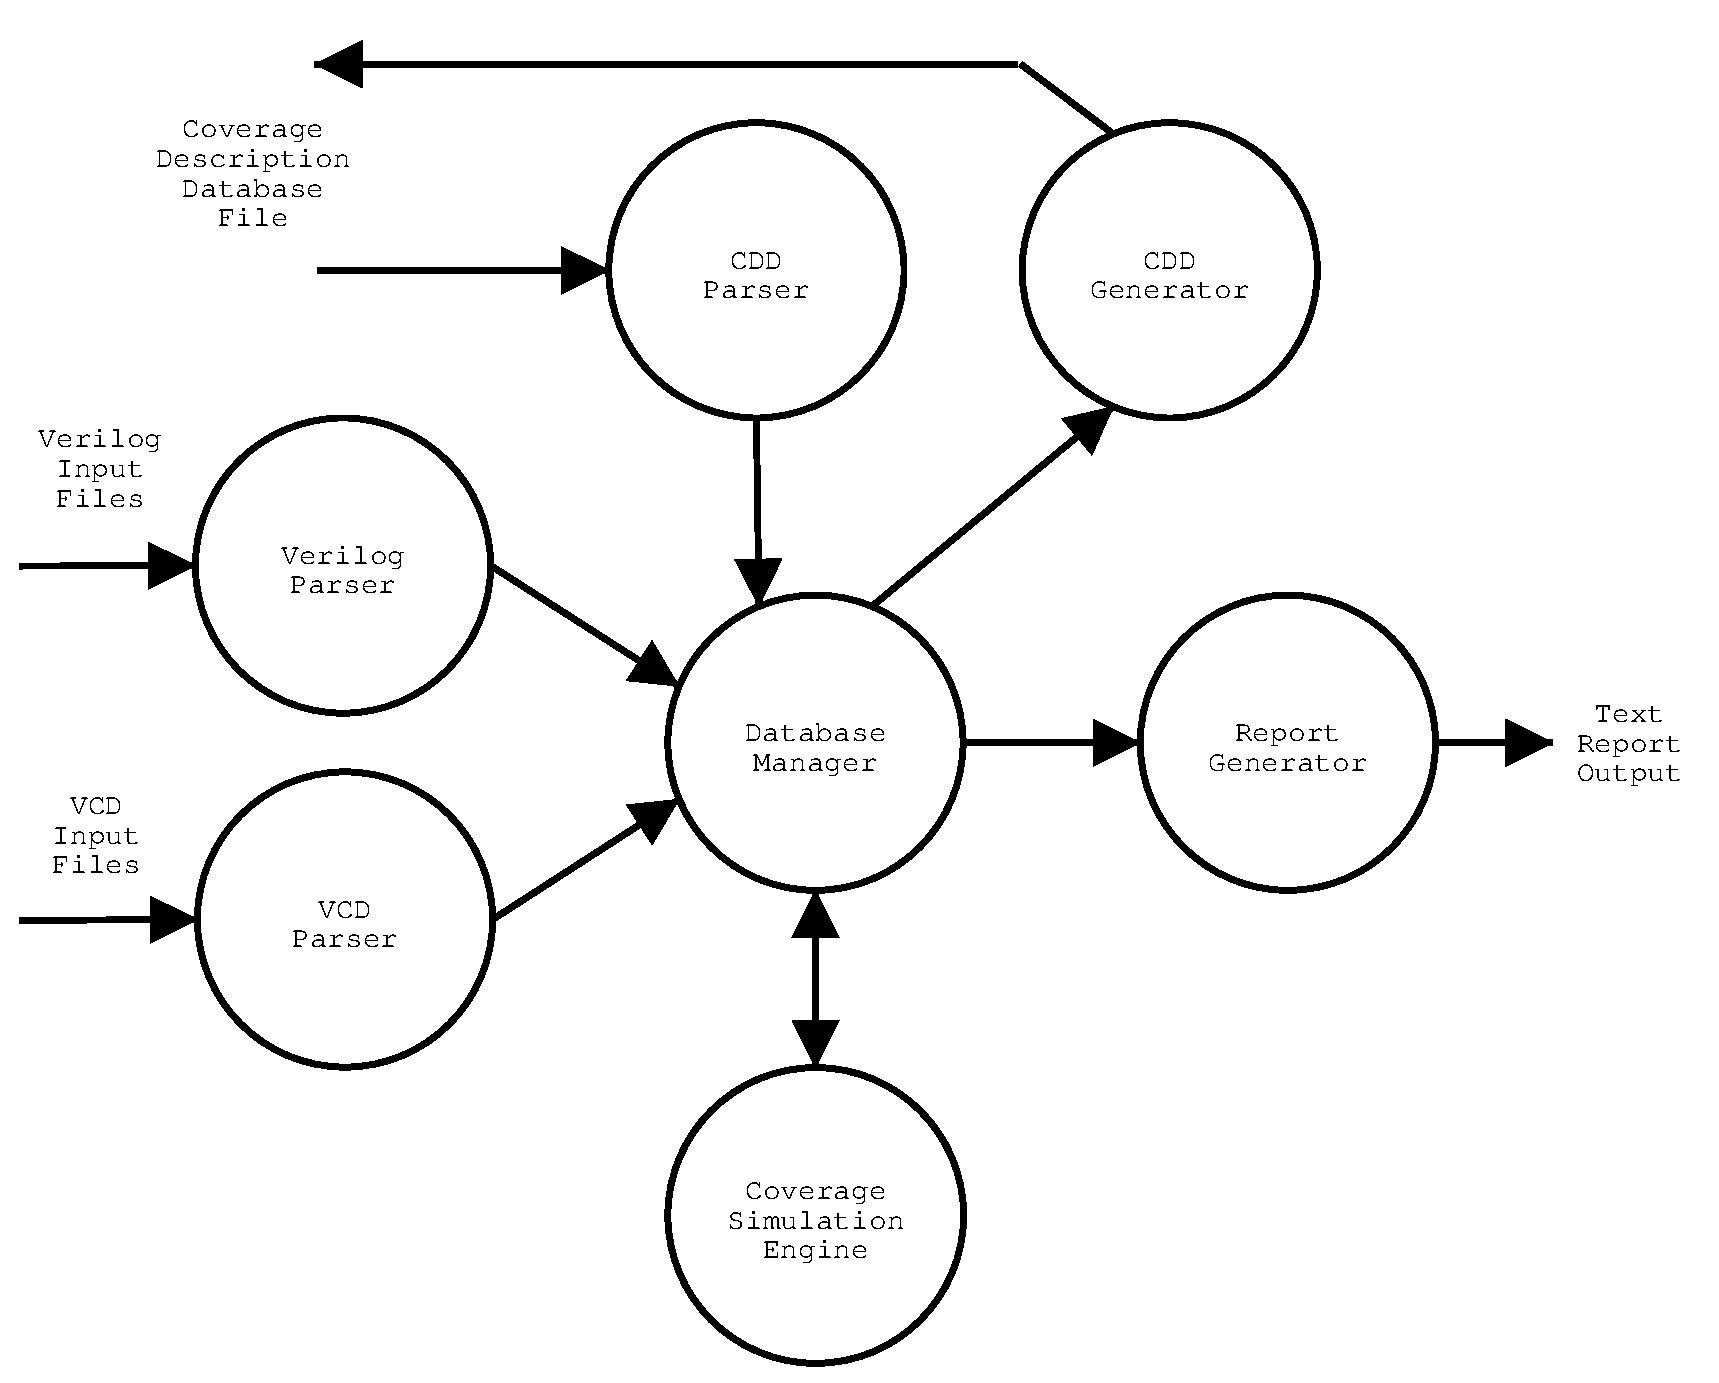
\includegraphics{big_picture.eps}\caption{Figure 1.  Data Flow Diagram}
\end{center}
\end{figure}
 

\begin{Desc}
\item[Section 5.2.  Functional Block Descriptions]\par
 The following subsections describes each of these functions/nodes in greater detail.\end{Desc}
\begin{Desc}
\item[Section 5.2.1.  Verilog Parser]\par
 The Verilog parser used by Covered consists of a Flex lexical analyzer lexer.l and  Bison parser parser.y . Both the lexer and parser where used from the Icarus Verilog project which can be accessed at

 {\tt http://icarus.com/eda/verilog/index.html}

 Though most of the structure of both of these files maintain their original appearance from the Icarus project, most of the internal rule code has been removed and re-implemented to suite Covered's needs from the parser. The parser and lexer work together as most language parsers do with the lexer reading in tokens of information from the input files and passing these tokens for the parser to match with pre-existing language rules. The reason for taking both the lexer and parser from the Icarus project is that the Icarus project is well-used by the g\-EDA community for Verilog simulation and passes in regression the IV testsuite. This testsuite is part of the Verilog testsuite for Covered and is available for download at

 {\tt http://ivtest.sourceforge.net}

 Using the Verilog directory and file pathnames specified on the command-line, Covered generates a list of files to search for Verilog module names. The first module name that Covered attempts to find is the top-level module targetted for coverage. This module name is also specified on the command-line with the {\tt -t} option. The lexer reads in the file and finds the name specified after the Verilog {\bf keyword} {\rm (p.\,\pageref{structkeyword})} {\tt {\bf module}}. If this module matches the top-level module name, the contents of the module are parsed. If the module name does not match the top-level module name, the lexer skips the body of the module until it  encounters the {\tt endmodule} {\bf keyword} {\rm (p.\,\pageref{structkeyword})}. If there are any more modules specified in the given file, these are parsed in the same fashion. If the end of the file has been reached and no module has been found that is needed, the Verilog file is placed at the end of the file  queue and the next file at the head of the queue is read in by the lexer.

 If the top-level module contains module instantiations that also need to be tested for coverage, these module names are placed at the tail of the needed module queue. When the needed module queue is empty, all modules have been found and parsed, and the parsing phase of the procedure is considered complete and successful.

 When the parser finds a match for one of its rules, an action is taken. This action is typically one of the following:

\begin{enumerate}
\item 
Create a new structure for data storage.\item 
Store a structure into one of the lists or trees for later retrieval.\item 
Manipulate a structure based on some information parsed.\item 
Display an error message due to finding code that is incorrect language structure.\end{enumerate}
\end{Desc}


 The Verilog parser only sends information to and gets information from the database manager. When parsing is complete, the database manager contains all of the information from the Verilog design which is stored in special containers which are organized by a group of trees and lists.



\begin{Desc}
\item[Section 5.2.2.  Database Manager]\par
 {\bf TBD}\end{Desc}


\begin{Desc}
\item[Section 5.2.3.  CDD Parser]\par
 The Coverage Description Database file, or CDD as it is referred to in this documentation, is a generalized description of a Verilog design that contains coverage-specific information as it pertains to that design. CDD files are in ASCII text format. The reasons for having this file format are three-fold.

\begin{enumerate}
\item 
Allow a way to store information about a particular design in a way that is compact and concise. It is understood that a CDD file may exist for an indeterminant amount of time so it is important that the file size be as small as possible while still carrying enough information to generate useful coverage reports.\item 
Create a standardized output format that is easy to parse (can be done with the sscanf utility in a straight-forward way) not requiring the use and overhead of another lexer  and parser. The standardization of the file format allows several CDDs to be easily merged and output in the same format.\item 
Create a format that is flexible enough to add new constructs as needed to support the growing Verilog language while not making it more difficult to parse.\end{enumerate}
\end{Desc}


 The generic output format for the CDD file is as follows:

 {\tt $<$unique\_\-numeric\_\-ID\_\-for\_\-construct$>$} {\tt $<$information\_\-about\_\-construct\_\-separated\_\-by\_\-spaces$>$}

 If a new construct needs to be added to the tool, one merely needs to select a unique ID for that construct and come up with a format for displaying the information for that construct so that it is separated by spaces or commas and contains only one ENDLINE character at the end of the line. Blank lines or comments are allowed within the file. The current constructs that are output to a CDD file by Covered are listed below along with their unique ID.

\begin{CompactItemize}
\item 
signal (1)\item 
expression (2)\item 
module (3)\item 
statement (4)\end{CompactItemize}


 The information format for each construct is listed with the description of the construct in the {\bf Section 6.  Coverage Development Reference} {\rm (p.\,\pageref{page_code_details})} section.

 Each line of the CDD file is read into memory by the CDD parser and the first value of the line (the unique construct ID) is used to call the {\tt db\_\-read} function of the associated construct. The construct then takes the initiative of decoding the rest of the line and storing its contents into the same set of lists and trees that the Verilog parser stores its information into. The end result of parsing in the CDD file is the same as parsing in a design by the Verilog parser. Once into memory, the information can be merged, simulated, or computed on by the report generator.



\begin{Desc}
\item[Section 5.2.4.  CDD Generator]\par
 The CDD generator is actually distributed among the various constructs that make up the CDD file. The main {\tt db\_\-write} function located in {\bf db.c} calls each of the construct's {\tt db\_\-write} functions which, in turn, output their information to the CDD file in their own format. After each of the stored constructs have written their information to the CDD file, it is closed by the {\tt db\_\-write} function. The end result is a CDD file that is in the same format as the CDD file that was read in by the CDD parser.\end{Desc}


\begin{Desc}
\item[Section 5.2.5.  VCD Parser]\par
 After a design or CDD has been stored internally into the database manager's memory, that memory may be merged with the data stored in another CDD, used to generate a report, or simulated with the use of the input from a VCD file that was created from the design loaded into the database manager's memory. In the last scenario, the VCD parser is invoked to read in the contents of the specified VCD dumpfile. The VCD parser can read in any VCD file that is output according to the VCD format. The format of VCD can be found at:

 {\tt http://www-ee.eng.hawaii.edu/$\sim$msmith/ASICs/HTML/Verilog/LRM/HTML/15/ch15.2.htm\#pgf\-Id=250}

 The VCD parser is written using a lexer and parser combination. The lexer (vcd\_\-lexer.l) is compiled using the Flex utility and the parser (vcd\_\-parser.y) is compiled using the  Bison utility.\end{Desc}


\begin{Desc}
\item[Section 5.2.6.  Coverage Simulation Engine]\par
 {\bf TBD}\end{Desc}


\begin{Desc}
\item[Section 5.2.7.  Report Generator]\par
 {\bf TBD}\end{Desc}


\begin{Desc}
\item[Section 5.3.  Covered Command Flow]\par
 {\bf TBD}\end{Desc}
\begin{Desc}
\item[Section 5.3.1.  Score Command]\par
 {\bf TBD}\end{Desc}


\begin{Desc}
\item[Section 5.3.2.  Merge Command]\par
 {\bf TBD}\end{Desc}


\begin{Desc}
\item[Section 5.3.3.  Report Command]\par
 {\bf TBD}\end{Desc}


\begin{Desc}
\item[Go To Section...]\par
\begin{CompactItemize}
\item 
{\bf Section 1.  Introduction} {\rm (p.\,\pageref{page_intro})}\item 
{\bf Section 2.  Project Plan} {\rm (p.\,\pageref{page_project_plan})}\item 
{\bf Section 3.  Coding Style Guidelines} {\rm (p.\,\pageref{page_code_style})}\item 
{\bf Section 4.  Development Tools} {\rm (p.\,\pageref{page_tools})}\item 
{\bf Section 6.  Coverage Development Reference} {\rm (p.\,\pageref{page_code_details})}\item 
{\bf Section 7.  Test and Checkout Procedure} {\rm (p.\,\pageref{page_testing})}\item 
{\bf Section 8.  Odds and Ends Information} {\rm (p.\,\pageref{page_misc})}\end{CompactItemize}
\end{Desc}

\section{Section 6.  Coverage Development Reference}\label{page_code_details}
\begin{Desc}
\item[Section 6.1. Extracted Documentation]\end{Desc}
\begin{Desc}
\item[]The following links will take you to the generated documentation for the project. This documentation is always in sync with the current CVS snapshot.\end{Desc}
\begin{Desc}
\item[]\begin{itemize}
\item {\tt Modules} - A list of related defines, structures, unions, etc.\item {\tt Structures and Unions} - A list of structures/union descriptions.\item {\tt File List} - A list of all source/header file descriptions.\item {\tt Function List} - A list of all function descriptions.\item {\tt File Members} - Descriptions of all file members for a given file.\item {\tt Bug List} - List of known bugs within the code for future fixes.\end{itemize}
\end{Desc}




\begin{Desc}
\item[Go To Section...]\begin{itemize}
\item {\bf Section 1.  Introduction}{\rm (p.\,\pageref{page_intro})}\item {\bf Section 2.  Project Plan}{\rm (p.\,\pageref{page_project_plan})}\item {\bf Section 3.  Coding Style Guidelines}{\rm (p.\,\pageref{page_code_style})}\item {\bf Section 4.  Development Tools}{\rm (p.\,\pageref{page_tools})}\item {\bf Section 5.  Project \char`\"{}Big Picture\char`\"{}}{\rm (p.\,\pageref{page_big_picture})}\item {\bf Section 7.  Test and Checkout Procedure}{\rm (p.\,\pageref{page_testing})}\item {\bf Section 8.  Debugging}{\rm (p.\,\pageref{page_debugging})}\item {\bf Section 9.  Odds and Ends Information}{\rm (p.\,\pageref{page_misc})} \end{itemize}
\end{Desc}

\section{Section 7.  Test and Checkout Procedure}\label{page_testing}
\begin{Desc}
\item[Section 7.1. Testing Methodology]Testing the Covered tool for general \char`\"{}goodness\char`\"{}, which is required for release, is accomplished with its own suite of C and Verilog diagnostics. These suite of tests are run in a regression manner; that is, each diagnostic is self-checking and run in serial order. The results of each diagnostic are output to standard output as well as an output file. After all diagnostics are run, the output file is grep'ed for the keyword \char`\"{}PASSED\char`\"{}. The number of diagnostics finishing the PASS message are compared against the total number of diagnostics. The results of which are output to standard output.\end{Desc}
\begin{Desc}
\item[]To release a new version of the tool for general consumption, the following testing procedures are required to occur prior to the release.\begin{enumerate}
\item New C/Verilog diagnostics are written to test new features of tool. These diagnostics will be self-contained and self-checking, displaying a message of \char`\"{}PASSED\char`\"{} if the diagnostic has successfully tested the feature under test or some message displaying the cause of failure. The failure message may not contain the keyword \char`\"{}PASSED\char`\"{} in its description.\item These newly written diagnostics are added to the regression suite, the list of which is maintained in the Makefile located in the diagnostic directory.\item A regression run is run in both the C diagnostic directory as well as the Verilog diagnostic directory.\item 100\% of the diagnostics in the regression suite result in a PASS message for both the C and Verilog directories.\end{enumerate}
\end{Desc}




\begin{Desc}
\item[Section 7.2. Testing Directories]The reason for having two directories for regression testing relies on the feature under test. Verilog diagnostics are condensed DUTs which only contain the required code for testing a particular syntax of the Verilog language to verify that Covered is able to correctly parse the code and generate the appropriate coverage results for that feature. All Verilog diagnostics are accompanied by a text file that is used for comparison purposes. The Makefile, after simulating the Verilog file, creating the dumpfile, generating the CDD and generating a verbose report based on the CDD will compare the generated report to the text file by performing a UNIX \char`\"{}diff\char`\"{} command. If the results of the \char`\"{}diff\char`\"{} are no differences between the two files, the Makefile will assume that the diagnostic has successfully passed and output the keyword \char`\"{}PASSED\char`\"{} to the output result file. If the results of \char`\"{}diff\char`\"{} show that there are differences between the two files, the Makefile will assume failure and output the keyword \char`\"{}FAILED\char`\"{} to the output result file.\end{Desc}
\begin{Desc}
\item[]C diagnostics exist to test certain functions of Covered rather than the entire tool itself. Many times it is impossible/impractical to create Verilog diagnostics that exercise certain functions within Covered to completion. In these cases, it is often easier to write more specialized tests that can more quickly manipulate inputs to functions and verify that all output values are correct. Examples of C diagnostics that currently exist in the C regression directory include tests of bitwise operators, mathematical functions, etc.\end{Desc}
\begin{Desc}
\item[]It is suggested that if functions can be adequately tested at a system level, that it be done so using Verilog diagnostics as these will get the most testing out of the entire tool. However, if functions are best tested in seclusion, it is suggested that the C testing environment be used.\end{Desc}




\begin{Desc}
\item[Section 7.3. Verilog Testing Procedure]{\bf TBD}  \end{Desc}




\begin{Desc}
\item[Go To Section...]\begin{itemize}
\item {\bf Section 1.  Introduction} \item {\bf Section 2.  Project Plan} \item {\bf Section 3.  Coding Style Guidelines} \item {\bf Section 4.  Development Tools} \item {\bf Section 5.  Project \char`\"{}Big Picture\char`\"{}} \item {\bf Section 6.  Coverage Development Reference} \item {\bf Section 8.  Odds and Ends Information} \end{itemize}
\end{Desc}

\section{Section 8.  Odds and Ends Information}\label{page_misc}
\begin{Desc}
\item[Section 8.1. Development Team]\begin{itemize}
\item Trevor Williams ({\tt trevorw@charter.net})\end{itemize}
\end{Desc}




\begin{Desc}
\item[Go To Section...]\begin{itemize}
\item {\bf Section 1.  Introduction} \item {\bf Section 2.  Project Plan} \item {\bf Section 3.  Coding Style Guidelines} \item {\bf Section 4.  Development Tools} \item {\bf Section 5.  Project \char`\"{}Big Picture\char`\"{}} \item {\bf Section 6.  Coverage Development Reference} \item {\bf Section 7.  Test and Checkout Procedure} \end{itemize}
\end{Desc}

\section{Bug List}\label{bug}
\begin{description}
\item[\label{_bug000003}
Member {\bf directory\_\-load}(char $\ast$dir, str\_\-link $\ast$ext\_\-head, str\_\-link $\ast$$\ast$file\_\-head, str\_\-link $\ast$$\ast$file\_\-tail) ]
Need to order files according to extension first instead of filename.\end{description}


\begin{description}
\item[\label{_bug000001}
Member {\bf do\_\-define}() ]
This strips trailing line comments out of the definition. It's not adequate as the \char`\"{}//\char`\"{} may have been quoted or commented, but it will do for now.\end{description}


\begin{description}
\item[\label{_bug000002}
Member {\bf signal\_\-db\_\-read}(char $\ast$$\ast$line, module $\ast$curr\_\-mod) ]
A signal will only look in the current module for a matching expression. In the case of a hierarchical reference, it is possible that an expression outside the current module is referencing this signal. We need to check for this case (hierarchical expression) and find the expression elsewhere.\end{description}
 
\printindex
\end{document}
